% ##############################################
% Start: Template Preamble
% ##############################################
%
\listfiles
% Documentclass definition
% KOMA-Script class 'scrbook'
% Link to the documentation:
%http://mirrors.ctan.org/macros/latex/contrib/koma-script/doc/scrguide.pdf
% CTAN: http://www.ctan.org/pkg/koma-script
\documentclass%
[%
paper=a4
,fontsize=11pt % common are 10, 11 or 12
,headings=big
,parskip
,numbers=noendperiod % 2.3.1 vs 2.3.1. (no dot after the last chapter number)
,twoside=true
,bibliography=totoc % Bibliography appears in Table of Contents (without a number)
,totoc=listof % List of Figures and List of Tables appear in Table of Contents
,version=last % Use latest version of the KOMA-Script
]%
{scrbook}


% Loading additional packages from the KOMA-Script family
% Special KOMA-Script package - I added it because I also use the float package in this template, see: 
% http://tex.stackexchange.com/questions/51867/koma-warning-about-toc
% CTAN: http://www.ctan.org/tex-archive/macros/latex/contrib/koma-script/doc
\usepackage{scrhack}

% Better support for marginnotes
% new command: \marginnote
% LaTeX standard command: \marginpar
% CTAN: http://www.ctan.org/pkg/marginnote
\usepackage{marginnote}

% Extended header and footer support
% CTAN: http://www.ctan.org/pkg/scrpage2
\usepackage[%
  	automark
  	,ilines
	,headsepline
	,footsepline
]{scrpage2}

% Page layout definition
% User friendly interface to change layout parameters
% CTAN: http://www.ctan.org/pkg/geometry
\usepackage{geometry}
\geometry{% siehe geometry.pdf (Figure 1)
	bottom=30mm,
	showframe=false, % For debugging: try true and see the layout frames
	%showframe=true, % For debugging: try true and see the layout frames
	margin=30mm,
	marginparsep=3mm,
	marginparwidth=20mm
}
%%Geometry different from master thesis... Check in formatAndDefs_original.tex


% Standard packages
% Input encoding is 'latin1' (Latin 1 - also known as ISO-8859-1)
% CTAN: http://www.ctan.org/pkg/inputenc
%
% A newer package is available - you may look into:
% \usepackage[x-iso-8859-1]{inputenc}
% CTAN: http://www.ctan.org/pkg/inputenx
\usepackage[latin1]{inputenc}%OK

% Font Encoding is 'T1' -- important for special characters such as Umlaute � or � and special characters like � (enje)
% CTAN: http://www.ctan.org/pkg/fontenc
\usepackage[T1]{fontenc, url}%OK
\usepackage[bitstream-charter]{mathdesign}

% Language support for 'english' (alternative 'ngerman' or 'french' for example)
% CTAN: http://www.ctan.org/pkg/babel
\usepackage[english]{babel} %OK
\usepackage[babel]{csquotes}
\usepackage{hyphenat}
\hyphenation{tem-pe-ra-tu-re}

% Doing calculations with LaTeX units -- needed for the vertical line in the footer
% CTAN: http://www.ctan.org/pkg/calc
\usepackage{calc}%OK

% Extended graphics support
% There is also a package named 'graphics' - watch out!
% CTAN: http://www.ctan.org/pkg/graphicx
\usepackage{graphicx}%OK

% Extendes support for floating objects (tables, figures), adds the [H] placing option (\begin{figure}[H]) which palces it "Here" (without any doubt).
% CTAN: http://www.ctan.org/pkg/float
\usepackage{float}

% Support for captions, subcaptions and subfigures
\usepackage[margin=20pt]{subcaption}
\usepackage{caption}
\captionsetup{justification=justified, format=hang}

% Extended color support
% I use the command \definecolor for example.
% Option 'Table': Load the colortbl package, in order to use the tools for coloring rows, columns, and cells within tables.
% CTAN: http://www.ctan.org/pkg/xcolor
\usepackage[table]{xcolor}

% Nice tables
% CTAN: http://www.ctan.org/pkg/booktabs
\usepackage{booktabs}%OK

% Better support for ragged left and right. Provides the commands \RaggedRight and \RaggedLeft.
% Standard LaTeX commands are \raggedright and \raggedleft
% http://www.ctan.org/pkg/ragged2e
\usepackage{ragged2e}

% Create function plots directly in LaTeX
% CTAN: http://www.ctan.org/pkg/pgfplots
\usepackage{pgfplots}
\pgfplotsset{compat=1.11}

%Create appendix
\usepackage[toc,page]{appendix}

% Create table of contents for each chapter
% CTAN: http://www.ctan.org/pkg/minitoc
\usepackage{minitoc}
\setcounter{minitocdepth}{2}

% Create nice bibliography
% CTAN: http://www.ctan.org/pkg/biblatex
\usepackage[backend=biber, bibstyle=authoryear, citestyle=authoryear-comp, sortcites, doi=true, dashed=false, indexing, backref=true, sorting=nyt, maxcitenames=1, maxbibnames=100, uniquelist=false, firstinits=true]{biblatex}%refsection=chapter, url=true, 
\setlength\bibitemsep{\baselineskip}
\DeclareNameFormat{coloured-family-given/given-family}{%
  \ifnumequal{\value{listcount}}{1}
    {\textcolor{myColorMainA}{%
     \ifgiveninits
       {\usebibmacro{name:family-given}
         {\namepartfamily}
         {\namepartgiveni}
         {\namepartprefix}
         {\namepartsuffix}}
       {\usebibmacro{name:family-given}
         {\namepartfamily}
         {\namepartgiven}
         {\namepartprefix}
         {\namepartsuffix}}%
     \ifboolexpe{%
       test {\ifdefvoid\namepartgiven}
       and
       test {\ifdefvoid\namepartprefix}}
       {}
       {\usebibmacro{name:revsdelim}}}}
    {\ifgiveninits
       {\usebibmacro{name:given-family}
         {\namepartfamily}
         {\namepartgiveni}
         {\namepartprefix}
         {\namepartsuffix}}
       {\usebibmacro{name:given-family}
         {\namepartfamily}
         {\namepartgiven}
         {\namepartprefix}
         {\namepartsuffix}}}%
  \usebibmacro{name:andothers}}
\DeclareNameAlias{sortname}{coloured-family-given/given-family}
\AtEveryCite{\color{myColorMainA}}
\usepackage{guit}
\urlstyle{sf}

%Create list of abbreviations and glossary
\usepackage[acronym, toc]{glossaries}

%Create analytical index
\usepackage[toc]{makeidx}
\DeclareIndexFieldFormat{indextitle}{}{}{}

%for schemes and pictures
\usepackage{tikz}
\usetikzlibrary{calc}

%Auxiliary packages for styling (from Nils)
\usepackage[protrusion=true,expansion=true]{microtype}
\usepackage[color=yellow,linecolor=white,textsize=footnotesize]{todonotes} % 
\usepackage{nicefrac}
\usepackage[binary-units=true]{siunitx}
\sisetup{per-mode = symbol-or-fraction}
\sisetup{detect-family = true}

%for nice tables
\usepackage{array}
\newcolumntype{P}[1]{>{\centering\arraybackslash}p{#1}}
\newcolumntype{M}[1]{>{\centering\arraybackslash}m{#1}}

\usepackage{longtable}
\usepackage{rotating}
\usepackage{tabularx}

\newcolumntype{s}{>{\hsize=.5\hsize}X}

\newcommand{\heading}[1]{\centering{\textbf{#1}}}

%%%Text specific features, like \textdegree{}
\usepackage{textcomp} 

% ####-Important-####
%
% Definition of the two main colors
% -----------------------
% The corresponding xcolor package ist loaded in the file
% 01_Preamble/StandardPackages.tex
%
% ####-Important-####
%\definecolor[named]{myColorMainA}{RGB}{0,26,153}%%BLU ACCESO
\definecolor[named]{myColorMainA}{HTML}{0B0B61}%%BLU SCURO
\definecolor[named]{myColorMainB}{RGB}{174,49,54}
% Customization of:
% - Floating Objects (Caption)
% - Table of Contents (TOC)
% - List of Figures
% - List of Tables
% - Headings (like chapter, section, etc.)
% ##############################################
% Start: Table of Contents (TOC) Customization
% ##############################################
%

% Level for numbered captions
\setcounter{secnumdepth}{5}

% Level of chapters that appear in Table of Contents
\setcounter{tocdepth}{5} % bis wohin ins Inhaltsverzeichnis aufnehmen
% -2 no caption at all
% -1 part
% 0  chapter
% 1  section    
% 2  subsection 
% 3  subsubsection
% 4  paragraph
% 5  subparagraph

% KOMA-Script code to adjust TOC
% Applying the color 'myColorMainA' which is defined in the main file (MainFile.tex)
\makeatletter
\addtokomafont{chapterentrypagenumber}{\color{myColorMainA}}
\addtokomafont{chapterentry}{\color{myColorMainA}}
\addtokomafont{partentrypagenumber}{\color{myColorMainA}}
\addtokomafont{partentry}{\color{myColorMainA}}
\makeatother

\makeatletter
\mtcsetfont{minitoc}{section}%
{\small\sffamily\upshape\bfseries\color{myColorMainA}}
\makeatother
\mtcsetrules{minitoc}{off}
\mtcsettitle{minitoc}{Contents}
\mtcsettitlefont{minitoc}{\large\sffamily\upshape\bfseries\color{myColorMainA}}

%
% #######################
% End: Table of Contents (TOC) Customization
% #######################

% ##############################################
% Start: Floating Object Customization
% ##############################################
%

% Extended support for captions of figures and tables etc.
% CTAN: http://www.ctan.org/pkg/caption
\usepackage[%
	font={small},
	labelfont={bf,sf},
	format=hang, % try plain or hang
	margin=5pt,
]{caption}
%

% #######################
% End: Floating Object Customization
% #######################

% ##############################################
% Start: Headings Customization
% ##############################################
%

% KOMA-Script code to customize the headings
% Applying the color 'myColorMainA' which is defined in the main file (MainFile.tex)
\addtokomafont{part}{\color{myColorMainA}}
\addtokomafont{chapter}{\color{myColorMainA}}
\addtokomafont{section}{\color{myColorMainA}}
\addtokomafont{subsection}{\color{myColorMainA}}
\addtokomafont{subsubsection}{\color{myColorMainA}}
\addtokomafont{paragraph}{\color{myColorMainA}}
\addtokomafont{subparagraph}{\color{myColorMainA}}

% #######################
% End: Headings Customization
% #######################


% Customization of the header, footer and teh margin note
\usepackage{titlesec}
% Custom command fpr the margin notes: \myMarginnote{Your Text}
% Comment on the \lineskiplimit=-\maxdimen:
% See http://tex.stackexchange.com/questions/49072/
% Without it the line spacing of the normal text was changed (ugly).
\newcommand{\myMarginnote}[1]{%
	\marginnote{% needs marginnote package
		\ifthispageodd{\RaggedRight}{\RaggedLeft}% needs ragged2e package
		\color{myColorMainA}%
		\lineskiplimit=-\maxdimen% 
		\normalfont\sffamily\scriptsize%
		#1}%
}

% ##############################################
% Start: Header and Footer Customization
% ##############################################
%

% KOMA-Script code for header and footer font
\setkomafont{pageheadfoot}{%
	\normalfont\sffamily\bfseries
	}
\setkomafont{pagefoot}{%
	\normalfont\sffamily
	}
\setkomafont{pagenumber}{%
	\normalfont\rmfamily
	}

% Define width of header
\setheadwidth[0pt]{textwithmarginpar}

% Define with of header line
\setheadsepline{0.4pt}

% Define width of footer
\setfootwidth[0pt]{text}
% Define with of footer line (here: no line)
\setfootsepline[text]{0pt}

% Some calculations
% calc package is needed which is loaded here: 01_Preamble/CommonPackages.tex
% If you want to understand the calculations visit:
% http://en.wikibooks.org/wiki/LaTeX/Page_Layout
\newlength{\myLenghthFootAbstand}
\setlength{\myLenghthFootAbstand}{\paperheight-1in-\topmargin- \headheight-\headsep-\textheight-\footskip}
\newlength{\myLenghthTemp}
\setlength{\myLenghthTemp}{\myLenghthFootAbstand+\baselineskip}

% Define content of header and footer
% Using some scrpage2 commands here. The scrpage2 package is loaded here: 01_Preamble/KOMA-Script-Packages.tex
% Some LaTeX magic...
% Clear all defaults
\clearscrheadfoot
% Header
\ohead{%
	\textcolor{myColorMainA}{\headmark}
	}
% Left (even page numbers) footer
\lefoot%
[% scrplain style (begin)
	\setlength{\unitlength}{\myLenghthFootAbstand}%
	\begin{picture}(0,0)%
		\put(0,-1)%
		{%
			\makebox(0,0)[lb]%
			{%
				\rule{0.4pt}{\myLenghthTemp}%
			}%
		}%
	\end{picture}\llap{\pagemark~}%
]% scrplain style (end)
%
{% scrheadings style (begin)
	\setlength{\unitlength}{\myLenghthFootAbstand}%
	\begin{picture}(0,0)%
		\put(0,-1)%
		{%
			\makebox(0,0)[lb]%
			{%
				\rule{0.4pt}{\myLenghthTemp}%
			}%
		}%
	\end{picture}\llap{\pagemark~}%
}% scrheadings style (end)

% Right (odd page numbers) footer
\rofoot%
[% scrplain style (begin)
	\rlap{~\pagemark}%%
	\setlength{\unitlength}{\myLenghthFootAbstand}%
	\begin{picture}(0,0)%
		\put(0,-1)%
		{%
			\makebox(0,0)[lb]%
			{%
				\rule{0.4pt}{\myLenghthTemp}%
			}%
		}%
	\end{picture}%
]% scrplain style (end)
%
{% scrplain style (begin)
	\rlap{~\pagemark}%%
	\setlength{\unitlength}{\myLenghthFootAbstand}%
	\begin{picture}(0,0)%
		\put(0,-1)%
		{%
			\makebox(0,0)[lb]%
			{%
				\rule{0.4pt}{\myLenghthTemp}%
			}%
		}%
	\end{picture}%
}% scrplain style (end)


\titlespacing*{\chapter}{0cm}{-1.cm}{-40pt}%pbk
\titleformat{\chapter}[display]{\Huge\filleft\sffamily\upshape\bfseries\color{myColorMainA}}{\color{myColorMainA}\normalfont\bf\fontfamily{put}\fontseries{b}\fontsize{95pt}{0pt}\selectfont\thechapter}{20pt}{}[\vspace{2ex}\filright\vspace{2ex}\glsresetall]
%\filleft\scshape


%
% #######################
% End: Header and Footer Customization
% #######################

% Optimize paragraphs (avoid overfull... warnings)
% This is an suggestion from Axel Reichert (LaTeX package author)
% See CTAN: http://www.ctan.org/author/reichert
% See CTAN: http://www.ctan.org/pkg/l2tabu-english (Cgapter: 1.8 Should I use \sloppy?)

\tolerance 1414
\hbadness 1414
\emergencystretch 1.5em
\hfuzz 0.3pt
\widowpenalty=10000
\vfuzz \hfuzz
\raggedbottom

% PDF related packages
% Package for PDF features such as bookmarks and hyperlinks. 
% Important: Should be loaded at the end.
% CTAN: http://www.ctan.org/pkg/hyperref
\usepackage[%
bookmarks, % Create bookmarks
bookmarksopen=true, % Unfold bookmatk tree in PDF viewer when document is opened
bookmarksopenlevel=1, % Level of unfolding
bookmarksnumbered=true, % Number bookmarks
hidelinks, % do not highlight hyperlinks -- looks ugly
% Ansicht beim �ffnen
pdfpagelabels=true, % See manual...
plainpages=false, % See manual...
hyperfootnotes=true, % Hyperlinks for footnotes
hyperindex=true, % Indexeintr�age verweisen auf Text
]{hyperref}

% PDF related packages
% Package to create test text -- just for demonstration purposes
% The command \blindtext produces a test text -- good for testing the layout
% CTAN: http://www.ctan.org/pkg/blindtext
\usepackage[]{blindtext}
% The custom command \myMarginnote is defined in the file: 
% 01_Preamble/HeaderFooterMarginnote.tex
\renewcommand{\blindmarkup}[1]{\myMarginnote{#1}}

% Custom commands for style
\DeclareMathVersion{mathchartertext}
\SetSymbolFont{letters}{mathchartertext}{OML}{mdbch}{m}{n}
\newcommand{\charmu}{\mathversion{mathchartertext}$\mu$\mathversion{normal}}
\newcommand{\charmum}{\mathversion{mathchartertext}$\mu$m\mathversion{normal}}
%\newcommand\ReferencesList{}
%\newcommand\AddtoRefsList[1]{\xdef\ReferencesList{\ReferencesList,#1}}
%\AtEveryCitekey{\AddtoRefsList{\thefield{entrykey}}}

%\makeatletter
%\patchcmd{\blx@addbackref@i}{\c@refsection}{\c@savedrefsection}{}{}

%\newcounter{savedrefsection}
%\newcommand\saverefsection{%
%  \protected@write\@mainaux{}{\string\setcounter{savedrefsection}{\the\c@refsection}}%
%}
%\makeatother

\newcounter{oldtocdepth}

\newcommand{\hidefromtoc}{%
  \setcounter{oldtocdepth}{\value{tocdepth}}%
  \addtocontents{toc}{\protect\setcounter{tocdepth}{-10}}%
}

\newcommand{\unhidefromtoc}{%
  \addtocontents{toc}{\protect\setcounter{tocdepth}{\value{oldtocdepth}}}%
}


\newcommand{\heading}[1]{\centering{\textbf{#1}}}
\newcommand{\xvarpm}[2]{\ooalign{\raisebox{-.5\height}{$#1-$}\cr\raisebox{.2\height}{$#1+$}\cr}}
\newcommand{\varpm}{\mathbin{\mathpalette\xvarpm\relax}}

%Title page Packages
\usepackage{amsmath}
\usepackage{tikz}
\usepackage{epigraph}
\usepackage{lipsum}
\usepackage{addfont}
\addfont{OT1}{cmpica}{\pica}

\renewcommand\epigraphflush{flushright}
\renewcommand\epigraphsize{\normalsize}
\setlength\epigraphwidth{0.7\textwidth}

%\definecolor{titlepagecolor}{cmyk}{1,.60,0,.40}
\definecolor{titlepagecolor}{RGB}{0,26,153}


%\DeclareFixedFont{\titlefont}{T1}{ppl}{b}{it}{0.5in}
\DeclareFixedFont{\titlefont}{T1}{qag}{b}{it}{0.43in}


\makeatletter
\def\printuniv{%
    {\large \@author}}
\makeatother
\author{%
    Universit\'{e} Claude Bernard Lyon 1\\
    Physics departement\\
    Doctoral school ED52: Physics and Astrophysics\vspace{20pt} \\
    }

% The following code is borrowed from: https://tex.stackexchange.com/a/86310/10898

\newcommand\titlepagedecoration{%
\begin{tikzpicture}[remember picture,overlay,shorten >= -10pt]

\coordinate (aux1) at ([yshift=-15pt]current page.north east);
\coordinate (aux2) at ([yshift=-380pt]current page.north east);
\coordinate (aux3) at ([xshift=-3.8cm]current page.north east);
\coordinate (aux4) at ([yshift=-150pt]current page.north east);

\begin{scope}[titlepagecolor,line width=12pt,rounded corners=12pt]
\draw
  (aux1) -- coordinate (a)
  ++(225:4) --
  ++(-45:5.1) coordinate (b);
\draw[shorten <= -10pt]
  (aux3) --
  (a) --
  (aux1);
\draw[opacity=0.3,titlepagecolor,shorten <= -10pt]
  (b) --
  ++(225:2.2) --
  ++(-45:2.2);
\end{scope}
%\draw[titlepagecolor,line width=8pt,rounded corners=8pt,shorten <= -10pt]
%  (aux4) --
 % ++(225:0.8) --
  %++(-45:0.8);
\begin{scope}[titlepagecolor!70,line width=6pt,rounded corners=8pt]
\draw[shorten <= -10pt]
  (aux2) --
  ++(225:3) coordinate[pos=0.45] (c) --
  ++(-45:3.1);
\draw
  (aux2) --
  (c) --
  ++(135:2.5) --
  ++(45:2.5) --
  ++(-45:2.5) coordinate[pos=0.3] (d);
\draw
  (d) -- +(45:1);
\end{scope}
\end{tikzpicture}%
}


%
% #######################
% End: Template Preamble
% #######################

%%Adding bibliography files
%\addbibresource{05_Bibliography/Biblio_13.bib}
\addbibresource{05_Bibliography/thesis.bib}

% ##############################################
% Start: Document
% ##############################################
%
% ------------------------------------------------------------------

% *****  ACRONYMS  ************

%%%%%%%%%%%%%%%%%% Institutions - collaborations - groups %%%%%%%%%%%%%%%%%%%%%%%%%
\newacronym{ipnl}{IPNL}{Institut de Physique Nucl\'{e}aire de Lyon, France}
\newacronym{lpsc}{LPSC}{Laboratoire de Physique Subatomique et Corpuscolaire, Grenoble, France}
\newacronym{lpc}{LPC}{Laboratoire de Physique de Clermont, France}
\newacronym{creatis}{CREATIS}{Centre de Recherche en Acquisition et Traitement de l'Image pour la Sant\'{e}, Lyon, France}
\newacronym{cppm}{CPPM}{Centre de Physique des Particules de Marseille, France}
\newacronym{clarys}{CLaRyS}{\textit{Contr\^{o}le en Ligne de l'hadronth\'{e}rapie par Rayonnements Secondaires}}
\newacronym{ganil}{GANIL}{Grand Accelerateur National d'Ions Lourds, Caen, France}
\newacronym{hit}{HIT}{Heidelberg Ion Therapy Center, Germany}
\newacronym{ipno}{IPNO}{Institut de Physique Nucl\'{e}aire d'Orsay, France}
\newacronym{lal}{LAL}{Laboratoire de l'Acc\'{e}l\'{e}rateur Lin\'{e}aire, Paris, France}
\newacronym{irfu}{IRFU}{Institut de Recherche sur les lois Fondamentales de l'Univers, Paris, France}
\newacronym{micrhau}{MICRHAU}{Micro-\'{e}lectronique RH\^{o}ne AUvergne}
\newacronym{cern}{CERN}{Conseil Europ\'{e}en pour la Recherche Nucl\'{e}aire, Geneva, Switzerland}
\newacronym{lhcb}{LHCb}{Large Hadron Collider beauty}
\newacronym{avirm}{AVIRM}{Application et Valorisation des Interactions Rayonnements-Mati\`{e}re}
\newacronym{psi}{PSI}{Paul Scherrer Institut, Villigen, Switzerland}
\newacronym{cal}{CAL}{Centre Antoine Lacassagne, Nice, France}
\newacronym{esrf}{ESRF}{European Synchrotron Radiation Facility, Grenoble, France}
\newacronym{infn}{INFN}{Istituto Nazionale di Fisica Nucleare, Italy}
\newacronym{adam}{A.D.A.M.}{Advanced Oncotherapy}
\newacronym{light}{LIGHT}{Linac for Image Guided HadronTherapy}
\newacronym{dwa}{DWA}{Dielectric Wall Accelerator}
\newacronym{llnl}{LLNL}{Lawrence Livermore National Laboratory, USA}
\newacronym{iba}{IBA}{Ion Beam Applications, Belgium}
\newacronym{cnao}{CNAO}{Centro Nazionale di Adroterapia Oncologica, Italy}
\newacronym{nirs}{NIRS}{National Institute of Radiological Sciences, Japan}
\newacronym{gsi}{GSI}{GSI Helmholtz Centre for Heavy Ion Research, Germany}
\newacronym{himac}{HIMAC}{Heavy Ion Medical Accelerator in Chiba, Japan}
\newacronym{nist}{NIST}{National Institute of Standards and Technology}
\newacronym{niu}{NIU}{Northern Illinois University}
\newacronym{fnal}{FNAL}{Fermi National Accelerator Laboratory}
\newacronym{llu}{LLU}{Loma Linda University}
\newacronym{ucsc}{UCSC}{University of California and Santa Cruz}
\newacronym{pravda}{PRaVDA}{Proton Radiotherapy Verification and Dosimetry Application}
\newacronym{lbl}{LBL}{Lawrence Berkeley Laboratory}
\newacronym{mgh}{MGH}{Massachusetts General Hospital}
\newacronym{inside}{INSIDE}{Innovative Solutions for Dosimetry in Hadrontherapy}
\newacronym{ptcog}{PTCOG}{Particle Therapy Co-Operative Group}
\newacronym{bnl}{BNL}{Brookhaven National Laboratory}
\newacronym{ge}{GE}{General Electric}
\newacronym{mit}{MIT}{Massachusetts Institute of Technology}

%%%%%%%%% Materials %%%%%%%%%%%%%%%%
\newacronym{bgo}{BGO}{Bismuth Germanium Oxide - Bi$\mathrm{_{12}}$GeO$\mathrm{_{20}}$}
\newacronym{cdte}{CdTe}{Cadmium Telluride}
\newacronym{cdznte}{CdZnTe}{Cadmium Zinc Telluride}
\newacronym{pmma}{PMMA}{Poly Methyl Metacrylate}
\newacronym{naitl}{NaI(Tl)}{Sodium Iodide doped with Thallium}
\newacronym{nai}{NaI}{Sodium Iodide}
\newacronym{lso}{LSO}{Cerium-doped Lutetium Oxyorthosilicate - Lu$\mathrm{_{2(1-x)}}$Ce$\mathrm{_{2x}}$SiO$\mathrm{_{4}}$}
\newacronym{lyso}{LYSO}{Lutetium-Yttrium OxyorthoSilicate - Lu$\mathrm{_{2(1-x)}}$Y$\mathrm{_{2x}}$SiO$\mathrm{_{5}}$}
\newacronym{baf2}{BaF$_2$}{Barium Fluoride}
\newacronym{csf}{CsF}{Cesium Fluoride}
\newacronym{cebr3}{CeBr$_3$}{Cerium Bromide}
\newacronym{labr3}{LaBr$_3$}{Lanthanum Bromide}
\newacronym{iod131}{$^{131}$I}{Iodine-131}
\newacronym{iod123}{$^{123}$I}{Iodine-123}
\newacronym{ind111}{$^{111}$In}{Indium-111}
\newacronym{ind131}{$^{131}$In}{Indium-131}
\newacronym{sod22}{$^{22}$Na}{Sodium-22}
\newacronym{cob60}{$^{60}$Co}{Cobalt-60}
\newacronym{cob57}{$^{57}$Co}{Cobalt-57}
\newacronym{ytt91m}{$^{91m}$Y}{Yttrium-91m}
\newacronym{fe59}{$^{59}$Fe}{Iron-59}
\newacronym{k42}{$^{42}$K}{Potassium-42}
\newacronym{lut177}{$^{177}$Lu}{Lutetium-177}
\newacronym{yagce}{YAG:Ce}{Cerium-activated yttrium aluminum garnet}
\newacronym{csi}{CsI}{Cesium Iodide}
\newacronym{lfs}{LFS}{Lutetium Fine Silicate}
\newacronym{pe}{PE}{Polyethylene}
\newacronym{gaggce}{GAGG:Ce}{Cerium doped Gadolinium Aluminium Gallium Garnet}


%%%%%%%%%%%% Detectors and utils %%%%%%%%%%%%%%%%%%%%%%
\newacronym{tof}{TOF}{Time-Of-Flight}
\newacronym{tot}{TOT}{Time-Over-Threshold}
\newacronym{fwhm}{FWHM}{Full Width at Half Maximum}
\newacronym{enc}{ENC}{Equivalent Noise Charge}
\newacronym{dssd}{DSSD}{Double-sided Silicon Strip Detector}
\newacronym{hegp}{HEGP}{High Energy General Purpose}
\newacronym{legp}{LEGP}{Low Energy General Purpose}
\newacronym{megp}{MEGP}{Medium Energy General Purpose}
\newacronym{lehr}{LEHR}{Low Energy High Resolution}
\newacronym{pm}{PM}{Photo-Multiplier}
\newacronym{sipm}{SiPM}{Silicon Photo-Multiplier}
\newacronym{fe}{FE}{Front-End}
\newacronym{asic}{ASIC}{Application-Specific Integrated Circuit}
\newacronym{led}{LED}{Light Emitting Diode}
\newacronym{adc}{ADC}{Analog-to-Digital Converter}
\newacronym{tdc}{TDC}{Time-to-Digital Converter}
\newacronym{nim}{NIM}{Nuclear Instrumentation Module}
\newacronym{atca}{ATCA}{Advanced Telecommunications Computing Architecture}
\newacronym{utca}{\charmu-TCA}{Micro Advanced Telecommunications Computing Architecture}
\newacronym{rms}{RMS}{Root Mean Square}
\newacronym{csa}{CSA}{Charge Sensitive Amplifier}
\newacronym{shs}{SHS}{Slow Shaper}
\newacronym{fpga}{FPGA}{Field Programmable Gate Array}
\newacronym{lvds}{LVDS}{Low-Voltage Differential Signaling}
\newacronym{cr-rc}{CR-RC}{Capacitor Resistor - Resistor Capacitor}
\newacronym{dll}{DLL}{Delay Locked Loop}
\newacronym{mch}{MCH}{\charmu-TCA Carrier HUB}
\newacronym{amc}{AMC}{Advanced Mezzanine Card}
\newacronym{asm}{ASM}{Analog Sampling Module}
\newacronym{thor}{THOR}{Trigger et HORloge}
\newacronym{udp}{UDP}{User Datagram Protocol}
\newacronym{tcp}{TCP}{Transmission Control Protocol}
\newacronym{ram}{RAM}{Random Access Memory}
\newacronym{vme}{VME}{VERSABUS Module Eurocard}
\newacronym{gsps}{Gsps}{Giga Sample Per Second}
\newacronym{msps}{Msps}{Mega Sample Per Second}
\newacronym{drs}{DRS}{Domino Ring Sampler}
\newacronym{dpga}{DPGA}{\textit{D\'{e}tecteur Pix\'{e}lis\'{e} de Grande Acceptance}}
\newacronym{usb}{USB}{Universal Serial Bus}
\newacronym{hsmc}{HSMC}{High-Speed Mezzanine Card}
\newacronym{sptr}{SPTR}{Single Photon Time Resolution}
\newacronym{mcs}{MCS}{Multiple Coulomb Scattering}
\newacronym{pg}{PG}{Prompt-Gamma}
\newacronym{em}{EM}{Electromagnetic}
\newacronym{ffag}{FFAG}{Fixed Field Alternating Gradient}
\newacronym{rf}{RF}{Radio-Frequency}
\newacronym{mlp}{MLP}{Most Likely Path}
\newacronym{mwpc}{MWPC}{Multi Wire Proportional Chamber}
\newacronym{gem}{GEM}{Gas Electron Multiplier}
\newacronym{ccd}{CCD}{Charge-Coupled Device}
\newacronym{ic}{IC}{Ionization Chamber}
\newacronym{ivi}{IVI}{Interaction Vertex Imaging}
\newacronym{cmos}{CMOS}{Complementary Metal Oxide Semiconductor}
\newacronym{icrp}{ICRP}{International Commission on Radiological Protection}
\newacronym{crt}{CRT}{Coincidence Resolution Time}
\newacronym{rpc}{RPC}{Resistive Plate Chamber}
\newacronym{lapd}{LAPD}{Large Area Pixelized Detector}
\newacronym{psf}{PSF}{Point-Spread Function}
\newacronym{doi}{DOI}{Depth Of Interaction}
\newacronym{lor}{LOR}{Line Of Response}
\newacronym{fov}{FOV}{Field Of View}
\newacronym{pgs}{PGS}{Prompt Gamma Spectroscopy}
\newacronym{pgt}{PGT}{Prompt Gamma Timing}
\newacronym{pgpi}{PGPI}{Prompt Gamma Peak Integral}

%%%%%%%%%%%% Code and software utils %%%%%%%%%%%%%%%%%%%%%
\newacronym{geant4}{GEANT4}{GEometry And Tracking 4}
\newacronym{lm-mlem}{LM-MLEM}{List Mode-Maximum Likelihood Expectation Maximization}
\newacronym{mlem}{MLEM}{Maximum Likelihood Expectation Maximization}
\newacronym{megalib}{MEGAlib}{Medium-Energy Gamma-ray Astronomy library}
\newacronym{gate}{GATE}{GEANT4 Application for Tomographic Emission}
\newacronym{lq}{LQ}{Linear-Quadratic}
\newacronym{lem}{LEM}{Local Effect Model}
\newacronym{mkm}{MKM}{Microdosimetric Kinetic Model}
\newacronym{fbp}{FBP}{Filtered Back-Projection}
\newacronym{art}{ART}{Algebraic Reconstruction Technique}
\newacronym{qmd}{QMD}{Quantum Molecular Dynamics}
\newacronym{inc}{INC}{Intra-nuclear Cascade}
\newacronym{bic}{BIC}{Binary Intra-nuclear Cascade}
\newacronym{bme}{BME}{Boltzmann-Master-Equation}
\newacronym{nurbs}{NURBS}{Non-Uniform Rational Basis Splines}
\newacronym{gpu}{GPU}{Graphics Processing Unit}
\newacronym{vrt}{VRT}{Variance Reduction Technique}
\newacronym{mc}{MC}{Monte Carlo}


%%%%%%%%%%%%% Physics %%%%%%%%%%%%%%%%%%%
\newacronym{pet}{PET}{Positron Emission Tomography}
\newacronym{spect}{SPECT}{Single Photon Emission Computed Tomography}
\newacronym{ct}{CT}{Computed Tomography}
\newacronym{mri}{MRI}{Magnetic Resonance Imaging}
\newacronym[plural=OAR, firstplural=Organs At Risk (OAR)]{oar}{OAR}{Organ At Risk}
\newacronym{csda}{CSDA}{Continuous Slowing Down Approach}
\newacronym{let}{LET}{Linear Energy Transfer}
\newacronym{rbe}{RBE}{Relative Biological Effectiveness}
\newacronym{bnct}{BNCT}{Boron Neutron Capture Therapy}
\newacronym{ptv}{PTV}{Planned Target Volume}
\newacronym{ctv}{CTV}{Clinical Target Volume}
\newacronym{sobp}{SOBP}{Spread-Out Bragg Peak}
\newacronym{impt}{IMPT}{Intensity-Modulated Particle Therapy}
\newacronym{imrt}{IMRT}{Intensity-Modulated RadioTherapy}
\newacronym{tps}{TPS}{Treatment-Planning System}
\newacronym{hu}{HU}{Hounsfield Units}
\newacronym{wepl}{WEPL}{Water-Equivalent Path Length}
\newacronym{rsp}{RSP}{Relative Stopping Power}
\newacronym{pct}{pCT}{proton Computed Tomography}
\newacronym{tcpr}{TCP}{Tumor Control Probability}
\newacronym{dsb}{DSB}{Double-Strand Break}
\newacronym{pide}{PIDE}{Particle Radiation Data Ensemble}
\newacronym{oer}{OER}{Oxygen Enhancement Ratio}
\newacronym{fdg}{FDG}{Fluoro-Deoxy-Glucose}
\newacronym{snr}{SNR}{Signal-to-Noise Ratio}
\newacronym{iconv}{IC}{Internal Conversion}
\newacronym{ec}{EC}{Electron Capture}
\newacronym{si}{SI}{Internation System of units}
\newacronym{roi}{ROI}{Region Of Interest}
\newacronym{fop}{FOP}{Fall-Off Position}


\makeglossaries

\makeindex

\begin{document}

\dominitoc
%\dominilof
%\dominilot

\pagenumbering{gobble}
%Thesis cover page
%\frontmatter
\hidefromtoc

%%%%%%%%%%%%%%%%
% modèle de page de garde pour une thèse de l'Université de Lyon (version de mars 2016)
% Attention ! Encodage UTF8 ! Sinon adapter en conséquence...
%%%%%%%%%%%%%%%%

%\documentclass[11pt,a4paper]{book}

%\usepackage[utf8]{inputenc}
%\usepackage[T1]{fontenc}
%\usepackage{graphicx}
%\usepackage[frenchb]{babel}
%\usepackage[inner=2.5cm,outer=2.5cm, top=2.5cm, bottom=2.5cm]{geometry}

\newgeometry{inner=2.5cm,outer=2.5cm, top=2.5cm, bottom=2.5cm}
\afterpage{\restoregeometry}

%\begin{document}

\setlength{\parindent}{0pt}
\thispagestyle{empty}


\begin{center}

\includegraphics[height=3cm]{03_GraphicFiles/pageDeGarde/logo} %le fichier "logo" doit être dans le même dossier que le fichier tex
\end{center}


\fontsize{11pt}{13pt}\selectfont
N\textsuperscript{o} d'ordre NNT : xxx

\vspace{1cm}

\begin{center}
\fontsize{14pt}{16pt}\selectfont
\textbf{\uppercase{Th\`{e}se de doctorat de l'universit\'{e} de Lyon}}\\
\fontsize{12pt}{14pt}\selectfont
op\'{e}r\'{e}e au sein de\\
\textbf{l'Universit\'{e} Claude Bernard Lyon 1}

\vspace{0.5cm}

\textbf{\'{E}cole Doctorale ED52\\% rectifier le numéro d'accréditation
Physique et Astrophysique de Lyon}% nom complet de l'école doctorale

\vspace{0.5cm}

\textbf{Sp\'{e}cialit\'{e} de doctorat :\\
Discipline : Physique m\'{e}dicale} % éventuellement


\vspace{1.5cm}

Soutenue publiquement \`{a} huis clos le 14/12/2018, par :\\
\fontsize{14pt}{16pt}\selectfont
\textbf{Mattia Fontana}

\vspace{1.5cm} % adapter à la longueur du titre

\rule[20pt]{\textwidth}{0.5pt}

\fontsize{25pt}{28pt}\selectfont
\textbf{Tests and characterization of gamma cameras for medical applications}\\
\vspace{0.5cm}
\fontsize{20pt}{23pt}\selectfont
\textbf{Test et caract\'{e}risation de cam\'{e}ras gamma pour le m\'{e}dical}

\rule{\textwidth}{0.5pt}

\vspace{2cm} % adapter à la longueur du titre
\end{center}

\fontsize{12pt}{14pt}\selectfont
Devant le jury compos\'{e} de :
\bigskip

\fontsize{11pt}{13pt}\selectfont

%Nom Pr\'{e}nom, grade/qualit\'{e}, \'{e}tablissement/entreprise \hfill Pr\'{e}sident(e) % mention "président" à ne préciser qu'après la soutenance

\bigskip

Llos\'{a} Gabriela, Professeur associ\'{e}e, IFIC - Institut de Fisica Corpuscolar, Paterna, Espagne \newline \hfill Rapporteure

Thirolf Peter, Professeur associ\'{e}, Fakult\"{a}t f\"{u}r Physik der LMU M\"{u}nchen - Lehrstuhl f\"{u}r Experimentalphysik - Medizinishce Physik, Garching, Allemagne \newline \hfill Rapporteur

Augier Corinne, Professeur, IPNL - Institut de Physique Nucl\'{e}aire de Lyon, France \newline \hfill Examinatrice

Cerello Piergiorgio, INFN - Istituto Nazionale di Fisica Nucleare, sezione di Torino, Italie \newline \hfill Examinateur

Morel Christian, Professeur, CPPM - Centre de Physique de Particules de Marseille - Aix-Marseille Universit\'{e}, Marseille, France \newline \hfill Examinateur

Rafecas Magdalena, Professeur, Institut f\"{u}r Medizintechnik - Universit\"{a}t zu L\"{u}beck, Allemagne \newline \hfill Examinatrice

\bigskip

L\'{e}tang Jean Michel, ma\^{i}tre de conf\'{e}rences, CREATIS - Centre de Recherche en Acquisition et Traitement de l'Image pour la Sant\'{e}, Lyon, France \newline \hfill Co-directeur de th\`{e}se % le cas échéant

Testa \'{E}tienne, ma\^{i}tre de conf\'{e}rences, IPNL - Institut de Physique Nucl\'{e}aire de Lyon, France \newline  \hfill Directeur de th\`{e}se

\bigskip

Dauvergne Denis, Directeur de Recherche CNRS, LPSC - Laboratoire de Physique Corpuscolaire de Grenoble, France \newline  \hfill Invit\'{e} % le cas échéant

\newpage

%\fontsize{12pt}{14pt}\selectfont   % si le document général n'est pas en police 11pt, décommenter et préciser la taille utilisée
% Suite du manuscrit
%\end{document}

% Empty page after title page
\cleardoublepage

%Change geometry after cover page

\newgeometry{% siehe geometry.pdf (Figure 1)
	bottom=30mm,
	showframe=false, % For debugging: try true and see the layout frames
	%showframe=true, % For debugging: try true and see the layout frames
	margin=30mm,
	marginparsep=3mm,
	marginparwidth=20mm
}

% Title page
%% Title page using \maketitle (a more flexible alternative is the titlepage environment)
\title{PHD Thesis}
\subtitle{Tests and characterization of gamma
cameras for ion beam therapy monitoring and nuclear
medicine application.}
\author{Mattia Fontana}
\date{03.12.2018}
\maketitle
\begin{titlepage}

\noindent
\textcolor{titlepagecolor}{\titlefont Tests and characterization \newline of gamma
cameras for \newline medical applications}\par
\epigraph{PhD Candidate}%
{\textsc{Mattia Fontana}}

\epigraph{Thesis directors}%
{\textsc{\'{E}tienne Testa} and \textsc{Jean Michel L\'{e}tang}}
\null\vfill
\vspace*{1cm}
\noindent
\hfill
\begin{minipage}{0.35\linewidth}
    \begin{flushright}
        \printuniv \\
        Defended on December the \nth{14} 2018
    \end{flushright}
\end{minipage}
%
\begin{minipage}{0.02\linewidth}
    \rule{1pt}{125pt}
\end{minipage}
\titlepagedecoration
\end{titlepage}



% Empty page after title page
\cleardoublepage

% Activate header and footer defined in the file:
% 01_Preamble/HeaderFooterMarginnote.tex
\pagestyle{scrheadings}

% Activate roman numbering 
\pagenumbering{roman}

% Start with page 1 (I)
\setcounter{page}{1}

% Prologue
%% Chapter without numbering but with appearance in the Table of Contents
% \addchap is a command from KOMA-Script
\addchap{Prologue}



% Abstract
% Chapter without numbering but with appearance in the Table of Contents
% \addchap is a command from KOMA-Script
%\addchap{Abstract}
\chapter*{Abstract}

\glsresetall


The application of nuclear and particle physics techniques in the field of medical diagnosis and pathology treatment is nowadays well-established in the clinical routine. In particular, several medical imaging techniques are based on the exploitation of elementary particles (\glsdesc{pet} (\gls{pet}), \glsdesc{spect} (\gls{spect}), \glsdesc{ct} (\gls{ct}) scans,  etc.), as well as treatment methods, mainly concerning cancer, which causes about 9 millions deaths per year all over the world.
     
In this context, ion beam therapy is a promising technique in cancer treatment because of the ion defined range and favorable dose delivery features with respect to standard photon radiotherapy. Strict and precise treatment planning and monitoring are now key points for the method developments and full exploitation. In particular, with the aim of optimizing the ion treatment effectiveness, the ion range monitoring is mandatory: different solutions have been explored, but an online treatment check is still a challenge. 
The ion beam treatment monitoring is mainly performed by means of secondary charged or neutral particles. In this context, the detection of the prompt-gammas (PG) emitted during treatments has proven its potential in the ion range control in real time. Since the first evidence of the existing correlation between the emitted gamma profile fall-off and the Bragg peak position, several groups are involved in research activities in order to develop and optimize instruments and methods with the aim of improving this monitoring technique.  Among the others, collimated and Compton cameras are being studied and optimized for this application. The same detectors can also be employed in nuclear medicine for the detection of the radioactive elements decay products.      

A collaboration of 4 laboratories in France, called \textit{\glsdesc{clarys}} (\gls{clarys}), is involved in the parallel development of two composite detectors for ion beam monitoring and nuclear medicine applications, and this thesis is carried out within this collaboration with the detectors clinical trial as final aim.

The development project started a few years ago and is now at the final stage. The two cameras have been designed according to simulation studies, and the different components are now under tests.
The collimated camera is composed of a multi-slit tungsten mechanical collimator, set in front of an absorber composed of 30 \glsdesc{bgo} (\gls{bgo}) blocks, for a total size of 210$\times$175$\times$30~mm$^{3}$; each block presents a streaked structure with a 8$\times$8 pseudo-pixel matrix and the signal is read-out by 4 photomultipliers. A $\sim$3~ns time resolution can be achieved on average for the prompt-gamma detection. The same absorber is part of the Compton camera, in addition to a scatterer section composed of 7 \glsdesc{dssd}s (\glspl{dssd}) 96$\times$96$\times$2~mm$^{3}$ each.
With the collimated camera, the parallel emitted photons are selected by the collimator and a mono-dimensional emission profile can be reconstructed. The Compton camera has a more efficient detection technique, thanks to the absence of a mechanical collimation system, and could potentially lead to 3D information via the reconstruction of the Compton cones. These features make it suitable for the application in nuclear medicine, in particular as an alternative to the present \gls{spect} collimated cameras, allowing for accurate and efficient image reconstructions with the usage of high energy gamma source, which should reduce image blurring effects due to attenuation in the patient and the total released dose with respect to the present clinical routine.
 
Concerning the monitoring of ion beam therapy treatments, an additional detector component is needed to temporally and spatially tag the incoming beam ions and help rejecting the relevant background (mostly due to neutrons) which strongly affects the prompt-gamma yield. A scintillating fiber tagging hodoscope, which can be coupled to both collimated and Compton camera, is under development: it is composed of 2 perpendicular planes of 128 scintillating fibers, read-out from both sides by 8 64-channel photomultipliers by Hamamatsu.
 
The thesis work consists in the critical evaluation, characterization and tuning of the different components, together with the associated electronics, and of the complete detectors on beam. In parallel, simulation studies can improve the detection technique and optimize the detector structure, as well as pave the way for further applications.

After a general introduction devoted to expose the thesis context in chapter~\ref{chap::1}, an overview of the instrumental and technical state of the art of the gamma cameras is given in chapter~\ref{chap::2}. Chapter~\ref{chap::3} focuses on the two cameras developed by the \gls{clarys}; the camera components are described in details, and all the characterization measurements performed during the three years of my PhD thesis are explained. Chapter~\ref{chap::4} and~\ref{chap::5} presents the simulation studies I performed with the aim of investigating the potential of the developed detectors for the application on ion beam therapy monitoring and nuclear medicine, respectively. The entire chapter~\ref{chap::6} is dedicated to the description of the tests performed on proton beams for the detector characterization measurements. The final chapter~\ref{chap::7} is used to summarize and discuss all the results obtained in this thesis work; furthermore, the perspectives of the project are fixed on a time-line for the next future, and new research directions emerging from the obtained results are proposed.        

\cleardoublepage

% Table of Contents and Lost of Figures/Tables
% Table of Contents (TOC)
% Special code so that it appears as a bookmark in the PDF viewer
\phantomsection
\pdfbookmark[0]{Table of Contents}{toc} % <-- Please edit the name if you want a different text as a bookbarl for the Table of Contents
\tableofcontents
% List of Figures
\listoffigures
% List of Tables
\listoftables 

% *****  ACRONYMS  ************

%%%%%%%%%%%%%%%%%% Institutions - collaborations - groups %%%%%%%%%%%%%%%%%%%%%%%%%
\newacronym{ipnl}{IPNL}{Institut de Physique Nucl\'{e}aire de Lyon, France}
\newacronym{lpsc}{LPSC}{Laboratoire de Physique Subatomique et Corpuscolaire, Grenoble, France}
\newacronym{lpc}{LPC}{Laboratoire de Physique de Clermont, France}
\newacronym{creatis}{CREATIS}{Centre de Recherche en Acquisition et Traitement de l'Image pour la Sant\'{e}, Lyon, France}
\newacronym{cppm}{CPPM}{Centre de Physique des Particules de Marseille, France}
\newacronym{clarys}{CLaRyS}{\textit{Contr\^{o}le en Ligne de l'hadronth\'{e}rapie par Rayonnements Secondaires}}
\newacronym{ganil}{GANIL}{Grand Accelerateur National d'Ions Lourds, Caen, France}
\newacronym{hit}{HIT}{Heidelberg Ion Therapy Center, Germany}
\newacronym{ipno}{IPNO}{Institut de Physique Nucl\'{e}aire d'Orsay, France}
\newacronym{lal}{LAL}{Laboratoire de l'Acc\'{e}l\'{e}rateur Lin\'{e}aire, Paris, France}
\newacronym{irfu}{IRFU}{Institut de Recherche sur les lois Fondamentales de l'Univers, Paris, France}
\newacronym{micrhau}{MICRHAU}{Micro-\'{e}lectronique RH\^{o}ne AUvergne}
\newacronym{cern}{CERN}{Conseil Europ\'{e}en pour la Recherche Nucl\'{e}aire, Geneva, Switzerland}
\newacronym{lhcb}{LHCb}{Large Hadron Collider beauty}
\newacronym{avirm}{AVIRM}{Application et Valorisation des Interactions Rayonnements-Mati\`{e}re}
\newacronym{psi}{PSI}{Paul Scherrer Institut, Villigen, Switzerland}
\newacronym{cal}{CAL}{Centre Antoine Lacassagne, Nice, France}
\newacronym{esrf}{ESRF}{European Synchrotron Radiation Facility, Grenoble, France}
\newacronym{infn}{INFN}{Istituto Nazionale di Fisica Nucleare, Italy}
\newacronym{adam}{A.D.A.M.}{Advanced Oncotherapy}
\newacronym{light}{LIGHT}{Linac for Image Guided HadronTherapy}
\newacronym{dwa}{DWA}{Dielectric Wall Accelerator}
\newacronym{llnl}{LLNL}{Lawrence Livermore National Laboratory, USA}
\newacronym{iba}{IBA}{Ion Beam Applications, Belgium}
\newacronym{cnao}{CNAO}{Centro Nazionale di Adroterapia Oncologica, Italy}
\newacronym{nirs}{NIRS}{National Institute of Radiological Sciences, Japan}
\newacronym{gsi}{GSI}{GSI Helmholtz Centre for Heavy Ion Research, Germany}
\newacronym{himac}{HIMAC}{Heavy Ion Medical Accelerator in Chiba, Japan}
\newacronym{nist}{NIST}{National Institute of Standards and Technology}
\newacronym{niu}{NIU}{Northern Illinois University}
\newacronym{fnal}{FNAL}{Fermi National Accelerator Laboratory}
\newacronym{llu}{LLU}{Loma Linda University}
\newacronym{ucsc}{UCSC}{University of California and Santa Cruz}
\newacronym{pravda}{PRaVDA}{Proton Radiotherapy Verification and Dosimetry Application}
\newacronym{lbl}{LBL}{Lawrence Berkeley Laboratory}
\newacronym{mgh}{MGH}{Massachusetts General Hospital}
\newacronym{inside}{INSIDE}{Innovative Solutions for Dosimetry in Hadrontherapy}
\newacronym{ptcog}{PTCOG}{Particle Therapy Co-Operative Group}
\newacronym{bnl}{BNL}{Brookhaven National Laboratory}
\newacronym{ge}{GE}{General Electric}
\newacronym{mit}{MIT}{Massachusetts Institute of Technology}

%%%%%%%%% Materials %%%%%%%%%%%%%%%%
\newacronym{bgo}{BGO}{Bismuth Germanium Oxide - Bi$\mathrm{_{12}}$GeO$\mathrm{_{20}}$}
\newacronym{cdte}{CdTe}{Cadmium Telluride}
\newacronym{cdznte}{CdZnTe}{Cadmium Zinc Telluride}
\newacronym{pmma}{PMMA}{Poly Methyl Metacrylate}
\newacronym{naitl}{NaI(Tl)}{Sodium Iodide doped with Thallium}
\newacronym{nai}{NaI}{Sodium Iodide}
\newacronym{lso}{LSO}{Cerium-doped Lutetium Oxyorthosilicate - Lu$\mathrm{_{2(1-x)}}$Ce$\mathrm{_{2x}}$SiO$\mathrm{_{4}}$}
\newacronym{lyso}{LYSO}{Lutetium-Yttrium OxyorthoSilicate - Lu$\mathrm{_{2(1-x)}}$Y$\mathrm{_{2x}}$SiO$\mathrm{_{5}}$}
\newacronym{baf2}{BaF$_2$}{Barium Fluoride}
\newacronym{csf}{CsF}{Cesium Fluoride}
\newacronym{cebr3}{CeBr$_3$}{Cerium Bromide}
\newacronym{labr3}{LaBr$_3$}{Lanthanum Bromide}
\newacronym{iod131}{$^{131}$I}{Iodine-131}
\newacronym{iod123}{$^{123}$I}{Iodine-123}
\newacronym{ind111}{$^{111}$In}{Indium-111}
\newacronym{ind131}{$^{131}$In}{Indium-131}
\newacronym{sod22}{$^{22}$Na}{Sodium-22}
\newacronym{cob60}{$^{60}$Co}{Cobalt-60}
\newacronym{cob57}{$^{57}$Co}{Cobalt-57}
\newacronym{ytt91m}{$^{91m}$Y}{Yttrium-91m}
\newacronym{fe59}{$^{59}$Fe}{Iron-59}
\newacronym{k42}{$^{42}$K}{Potassium-42}
\newacronym{lut177}{$^{177}$Lu}{Lutetium-177}
\newacronym{yagce}{YAG:Ce}{Cerium-activated yttrium aluminum garnet}
\newacronym{csi}{CsI}{Cesium Iodide}
\newacronym{lfs}{LFS}{Lutetium Fine Silicate}
\newacronym{pe}{PE}{Polyethylene}
\newacronym{gaggce}{GAGG:Ce}{Cerium doped Gadolinium Aluminium Gallium Garnet}


%%%%%%%%%%%% Detectors and utils %%%%%%%%%%%%%%%%%%%%%%
\newacronym{tof}{TOF}{Time-Of-Flight}
\newacronym{tot}{TOT}{Time-Over-Threshold}
\newacronym{fwhm}{FWHM}{Full Width at Half Maximum}
\newacronym{enc}{ENC}{Equivalent Noise Charge}
\newacronym{dssd}{DSSD}{Double-sided Silicon Strip Detector}
\newacronym{hegp}{HEGP}{High Energy General Purpose}
\newacronym{legp}{LEGP}{Low Energy General Purpose}
\newacronym{megp}{MEGP}{Medium Energy General Purpose}
\newacronym{lehr}{LEHR}{Low Energy High Resolution}
\newacronym{pm}{PM}{Photo-Multiplier}
\newacronym{sipm}{SiPM}{Silicon Photo-Multiplier}
\newacronym{fe}{FE}{Front-End}
\newacronym{asic}{ASIC}{Application-Specific Integrated Circuit}
\newacronym{led}{LED}{Light Emitting Diode}
\newacronym{adc}{ADC}{Analog-to-Digital Converter}
\newacronym{tdc}{TDC}{Time-to-Digital Converter}
\newacronym{nim}{NIM}{Nuclear Instrumentation Module}
\newacronym{atca}{ATCA}{Advanced Telecommunications Computing Architecture}
\newacronym{utca}{\charmu-TCA}{Micro Advanced Telecommunications Computing Architecture}
\newacronym{rms}{RMS}{Root Mean Square}
\newacronym{csa}{CSA}{Charge Sensitive Amplifier}
\newacronym{shs}{SHS}{Slow Shaper}
\newacronym{fpga}{FPGA}{Field Programmable Gate Array}
\newacronym{lvds}{LVDS}{Low-Voltage Differential Signaling}
\newacronym{cr-rc}{CR-RC}{Capacitor Resistor - Resistor Capacitor}
\newacronym{dll}{DLL}{Delay Locked Loop}
\newacronym{mch}{MCH}{\charmu-TCA Carrier HUB}
\newacronym{amc}{AMC}{Advanced Mezzanine Card}
\newacronym{asm}{ASM}{Analog Sampling Module}
\newacronym{thor}{THOR}{Trigger et HORloge}
\newacronym{udp}{UDP}{User Datagram Protocol}
\newacronym{tcp}{TCP}{Transmission Control Protocol}
\newacronym{ram}{RAM}{Random Access Memory}
\newacronym{vme}{VME}{VERSABUS Module Eurocard}
\newacronym{gsps}{Gsps}{Giga Sample Per Second}
\newacronym{msps}{Msps}{Mega Sample Per Second}
\newacronym{drs}{DRS}{Domino Ring Sampler}
\newacronym{dpga}{DPGA}{\textit{D\'{e}tecteur Pix\'{e}lis\'{e} de Grande Acceptance}}
\newacronym{usb}{USB}{Universal Serial Bus}
\newacronym{hsmc}{HSMC}{High-Speed Mezzanine Card}
\newacronym{sptr}{SPTR}{Single Photon Time Resolution}
\newacronym{mcs}{MCS}{Multiple Coulomb Scattering}
\newacronym{pg}{PG}{Prompt-Gamma}
\newacronym{em}{EM}{Electromagnetic}
\newacronym{ffag}{FFAG}{Fixed Field Alternating Gradient}
\newacronym{rf}{RF}{Radio-Frequency}
\newacronym{mlp}{MLP}{Most Likely Path}
\newacronym{mwpc}{MWPC}{Multi Wire Proportional Chamber}
\newacronym{gem}{GEM}{Gas Electron Multiplier}
\newacronym{ccd}{CCD}{Charge-Coupled Device}
\newacronym{ic}{IC}{Ionization Chamber}
\newacronym{ivi}{IVI}{Interaction Vertex Imaging}
\newacronym{cmos}{CMOS}{Complementary Metal Oxide Semiconductor}
\newacronym{icrp}{ICRP}{International Commission on Radiological Protection}
\newacronym{crt}{CRT}{Coincidence Resolution Time}
\newacronym{rpc}{RPC}{Resistive Plate Chamber}
\newacronym{lapd}{LAPD}{Large Area Pixelized Detector}
\newacronym{psf}{PSF}{Point-Spread Function}
\newacronym{doi}{DOI}{Depth Of Interaction}
\newacronym{lor}{LOR}{Line Of Response}
\newacronym{fov}{FOV}{Field Of View}
\newacronym{pgs}{PGS}{Prompt Gamma Spectroscopy}
\newacronym{pgt}{PGT}{Prompt Gamma Timing}
\newacronym{pgpi}{PGPI}{Prompt Gamma Peak Integral}

%%%%%%%%%%%% Code and software utils %%%%%%%%%%%%%%%%%%%%%
\newacronym{geant4}{GEANT4}{GEometry And Tracking 4}
\newacronym{lm-mlem}{LM-MLEM}{List Mode-Maximum Likelihood Expectation Maximization}
\newacronym{mlem}{MLEM}{Maximum Likelihood Expectation Maximization}
\newacronym{megalib}{MEGAlib}{Medium-Energy Gamma-ray Astronomy library}
\newacronym{gate}{GATE}{GEANT4 Application for Tomographic Emission}
\newacronym{lq}{LQ}{Linear-Quadratic}
\newacronym{lem}{LEM}{Local Effect Model}
\newacronym{mkm}{MKM}{Microdosimetric Kinetic Model}
\newacronym{fbp}{FBP}{Filtered Back-Projection}
\newacronym{art}{ART}{Algebraic Reconstruction Technique}
\newacronym{qmd}{QMD}{Quantum Molecular Dynamics}
\newacronym{inc}{INC}{Intra-nuclear Cascade}
\newacronym{bic}{BIC}{Binary Intra-nuclear Cascade}
\newacronym{bme}{BME}{Boltzmann-Master-Equation}
\newacronym{nurbs}{NURBS}{Non-Uniform Rational Basis Splines}
\newacronym{gpu}{GPU}{Graphics Processing Unit}
\newacronym{vrt}{VRT}{Variance Reduction Technique}
\newacronym{mc}{MC}{Monte Carlo}


%%%%%%%%%%%%% Physics %%%%%%%%%%%%%%%%%%%
\newacronym{pet}{PET}{Positron Emission Tomography}
\newacronym{spect}{SPECT}{Single Photon Emission Computed Tomography}
\newacronym{ct}{CT}{Computed Tomography}
\newacronym{mri}{MRI}{Magnetic Resonance Imaging}
\newacronym[plural=OAR, firstplural=Organs At Risk (OAR)]{oar}{OAR}{Organ At Risk}
\newacronym{csda}{CSDA}{Continuous Slowing Down Approach}
\newacronym{let}{LET}{Linear Energy Transfer}
\newacronym{rbe}{RBE}{Relative Biological Effectiveness}
\newacronym{bnct}{BNCT}{Boron Neutron Capture Therapy}
\newacronym{ptv}{PTV}{Planned Target Volume}
\newacronym{ctv}{CTV}{Clinical Target Volume}
\newacronym{sobp}{SOBP}{Spread-Out Bragg Peak}
\newacronym{impt}{IMPT}{Intensity-Modulated Particle Therapy}
\newacronym{imrt}{IMRT}{Intensity-Modulated RadioTherapy}
\newacronym{tps}{TPS}{Treatment-Planning System}
\newacronym{hu}{HU}{Hounsfield Units}
\newacronym{wepl}{WEPL}{Water-Equivalent Path Length}
\newacronym{rsp}{RSP}{Relative Stopping Power}
\newacronym{pct}{pCT}{proton Computed Tomography}
\newacronym{tcpr}{TCP}{Tumor Control Probability}
\newacronym{dsb}{DSB}{Double-Strand Break}
\newacronym{pide}{PIDE}{Particle Radiation Data Ensemble}
\newacronym{oer}{OER}{Oxygen Enhancement Ratio}
\newacronym{fdg}{FDG}{Fluoro-Deoxy-Glucose}
\newacronym{snr}{SNR}{Signal-to-Noise Ratio}
\newacronym{iconv}{IC}{Internal Conversion}
\newacronym{ec}{EC}{Electron Capture}
\newacronym{si}{SI}{Internation System of units}
\newacronym{roi}{ROI}{Region Of Interest}
\newacronym{fop}{FOP}{Fall-Off Position}


\makeglossaries


\cleardoublepage

% Activate arabic numbering 
\pagenumbering{arabic}

% Start with page 1
\setcounter{page}{1}

\unhidefromtoc

% Prologue
% Chapter without numbering but with appearance in the Table of Contents
% \addchap is a command from KOMA-Script
\addchap{Prologue}



% Introduction
\chapter{Context}\label{chap::1}

\vfill

\minitoc

\newpage

\glsresetall

The application of physics concepts and techniques to the field of health-care is nowadays well-established in the clinical routine. Even if physical techniques have been used in medicine from the earliest time~\parencite{Duck2014}, the discipline today known as \enquote{medical physics} emerged and grown in the past century thanks to the increasing knowledge and use of ionizing radiations both for diagnosis and disease treatment. In the late \nth{19} century, the x-ray discovery by R\"{o}ntgen, the radioactivity discovery by Henri Becquerel, and the radium and radioactive isotopes studies by Pierre and Marie Curie paved the way to the whole medical physics practice of the next century, where x-ray imaging and radiotherapy were soon established. Only three weeks after the discovery of the x-rays, Robert Jones and Oliver Lodge imaged with x-rays a boy's hand~\parencite{Cantor1988}, officially starting the diagnostic application of such a radiation. Following the first successes, more attention was given to radio-protection and dosimetry studies, and the investigations focused on new ways to use radioactive tracers for imaging purpose; this finally led to the birth of nuclear medicine, with the clinical use of the radioisotope \gls{ind131} in 1939~\parencite{Kereiakes1987}. Nuclear medicine rapidly gained importance in the diagnosis clinical panorama, also thanks to the introduction of new detectors, such as the Anger camera introduced in the '60s, and new imaging techniques, such as the detection of photons from positron annihilation (\gls{pet}). Moreover, several alternative methods were proposed or implemented for diagnosis (\gls{mri}, ultrasounds, etc.). In parallel, x-rays were soon employed also for tumor treatment: already in 1896, Emil Grubbe irradiated a woman with breast cancer~\parencite{Evans1951}, and in the same year in Lyon a patient with a stomach cancer has been treated by Victor Despeignes~\parencite{Despeignes1896, Foray2016}. One year later, a skin tumor was successfully irradiated in Vienna using x-rays. Thanks to the invention of the klystron, and, later, of the so-called \enquote{magnetron}, by the Varian brothers with William Webster Hansen, the radiotherapy could spread and become a clinical reality; more refined treatment techniques were then introduced with the development of commercial particle accelerators after World War 2~\parencite{Keevil2012}. 

At present days, the medical physics progress strongly relies on technological development and computer science, which already revolutionized several fields of science. In particular, cancer research is now a key area for technical and technological development, concerning both diagnosis and treatment~\parencite{Webb2009}. Cancer continues to be one of the major issues in the medical scenario: it is at present the second cause of death worldwide, but it is expected to surpass heart diseases and become the main killer in the next tens of years~\parencite{Jemal2010, Thun2010}. The last two decades saw important improvements in radiotherapy techniques and machines, with more precise dose planning and delivery, which enhanced the patient survival and strongly reduced the impact of radiations on healthy tissues. This was possible also thanks to refined imaging technologies, allowing for an accurate tumor volume definition, as well as for image-guided treatments. In this scenario, ion beam therapy, already proposed in the middle of the past century, is rapidly spreading thanks to novel beam delivery technologies, able to relatively reduce the treatment costs and allowing for a commercial diffusion of this treatment method (which is still very limited with respect to standard radiotherapy). Notwithstanding the remarkable steps forward disclosed in the last years, there is still wide room for improvements in this field, which mainly requires strong imaging basis in order to fully profit of the treatment technique potential.

The work presented in this document has been carried out in this context and mainly deals with the development of gamma imaging detectors to be applied in the field of quality assurance for ion beam treatment. Furthermore, the same detectors have been applied to the nuclear medicine field in simulation, with the aim of assessing its possible clinical implementation for a future development of the nuclear medicine clinical routine. 

In the following sections, a general overview of the two main domains concerned in this thesis work is given. 

\section{Ion beam therapy}\label{chap1::sec::ionBeamTher}
Radiation treatment is an essential component of the tumor therapy, being the second most applied and successful kind of therapy after surgery~\parencite{Schardt2010}. The majority of patients with localized malignant tumors are treated with radiations~\parencite{Durante2009, Baskar2012, Moding2013}, applied in several fractions in different days in order to reduce the damages to normal tissues~\parencite{Bentzen2006}. The most of the patients treated with radio-therapy techniques receives standard photon treatments, with x-rays coming from linear electron accelerators; a small percentage undergoes specialized gamma treatments like gamma knife irradiations, again using x-ray beams from linear electron accelerators, or brachytherapy. About 1~\% of the radiotherapy patients are irradiated with charged particle beams, with the so-called ion beam therapy~\parencite{Durante2016}.

Ion beam therapy, or \enquote{hadrontherapy}, is a cancer radiation treatment method based on light ion beams instead of photons. It was first proposed by Wilson in 1946 in a famous seminal paper~\parencite{Wilson1946}; the author was asked by its director Ernest Lawrence to clarify the stopping process of protons in matter. Thanks to measurements at the Berkeley cyclotron, he highlighted the physical principles and the possible benefits driven by the implementation of such a kind of radiation in clinical treatments, with particular focus on the simple case of protons and some considerations about heavier ions, like alpha particles and carbon ions.  At that time, the accelerator technologies were still under development after the invention of the cyclotron by Ernest O. Lawrence in 1930, which allowed to increase the range of charged particles in matter, in particular in cells and human tissues, and the treatment-required beam energy was about to be reached. Pioneering studies of the biomedical applications of accelerated hadron beams were performed by Cornelius Tobias in 1948~\parencite{Blakely2009} in Berkeley (USA), and the first patients have been treated almost ten years later in the same laboratory by Lawrence and Tobias~\parencite{Tobias1955, Tobias1958} with protons and, later on, with He ions~\parencite{Halperin2006}. New accelerators in four continents were used to continue the quest started in Berkeley, and the experience was extended to carbon ion beams from 1994 in Japan (\gls{himac}), and Germany (Heidelberg - \gls{hit}). 

Nowadays clinical adapted machines are well-established on the market, making ion beam therapy emerging as a wide-spread technique in the every-day cancer treatment routine all over the world. Starting from the early 2000's, many new treatment centers have been designed and built, mainly in Europe and Japan. An intense research effort has been dedicated to this field in the last decades; in addition to considerable improvements achieved in the accelerator technologies, new and refined imaging techniques allowed for important enhancement in the treatment planning, also supported by the continuous development of computer science and the growth of calculation power. In parallel, the biological implications of ion irradiation has been deeply investigated~\parencite{Tobias1982, Brahme2004, Friedrich2012, }. Moreover, since more and more patients are treated every year with this technique, more clinical data are at present available for further study and the connection between physicists and physicians is strongly progressing both in the research field and in treatment practice. Several advancements are expected in the next years, following the extensive research work carried out by several groups in the world. In the following paragraph, the basic physical principles and features of this treatment method are explained, and advantages and drawbacks with respect to standard radiotherapy techniques are analyzed. After that, the need for ion range verification is discussed and detailed in order to reach the main topic for this thesis: the prompt-gamma detection.   

\subsection{Physics of ion beam therapy}\label{chap1::subsec::Physics}
The physics rationale of ion beam therapy is extensively described in all its peculiar aspects in several review, such as~\cite{Lomax2009, Belkic2010, Schardt2010, Bichsel2013, Nupecc2014,  Newhauser2015, Durante2016}. In the following, the physical basis of this tumor treatment technique is highlighted.
 
Charged nuclear particle beams at relatively high energy show a characteristic depth-dose distribution in matter which makes them suitable for the application in cancer treatment as a valid alternative to standard photon therapy (x-ray or megavolt beams), bringing several advantages to the patient side. The peculiar energy deposition profile (\enquote{Bragg curve}) is named for Sir William Henri Bragg, who investigated the slowing-down process of $\mathrm{\alpha}$ particles in air~\parencite{Bragg1904, Bragg1905}. 
Low-energy (x-rays) and high-energy photons traversing the patient body deposit their energy by interacting with the target atomic electrons (mainly by Compton interaction), with the deposited dose decreasing at increasing depth after a build-up region (mainly due to forward scattered Compton electrons). Even if the entrance surface (the skin for a patient) can be spared thanks to this build-up region, with a dose peak shift of a few centimeters, a high relative dose is delivered to the tissues along the whole beam path. In order to maximize the tumor volume-to-healthy tissue dose ratio, a standard photon treatment always foresees several irradiation fields from different entrance points and angles (see \figurename~\ref{chap1::fig::XraysCionsFields}, left). This energy deposit behavior is common to all neutral particles, as shown in the first two boxes in \figurename~\ref{chap1::fig::Depth-doseProf} where the depth-dose profiles of photons at various energies and neutrons in water are presented. 
In contrast to neutral particles, the energy deposited per track unit increases for increasing depth for the charged ones: in the remaining four boxes of \figurename~\ref{chap1::fig::Depth-doseProf} the depth-dose profile in water is shown for electrons, pions, protons and neon ions; it is characterized by an entrance low relative dose \textit{plateau} and by a narrow high deposited dose peak at the end of the range (in the last few millimeters), called \enquote{Bragg peak}. The high-dose peak is sharper the more massive is the particle, as clear from \figurename~\ref{chap1::fig::Depth-doseProf}, where the different species are sorted by increasing mass. As for protons and heavier ions, their clinical interest for the treatment of deep-seated tumors appears clearly from the above considerations: a nuclear particle beam is able to deliver a reduced dose to the healthy tissues surrounding the target volume, where the dose is concentrated. This allows for the treatment of tumor volumes close to \glspl{oar}, also with limited irradiation angles with respect to photons, as shown in the right part of \figurename~\ref{chap1::fig::XraysCionsFields}, where the planning for a carbon ion treatment of a lung cancer with only three irradiation fields is depicted. 

\begin{figure}[!htbp]
\centering
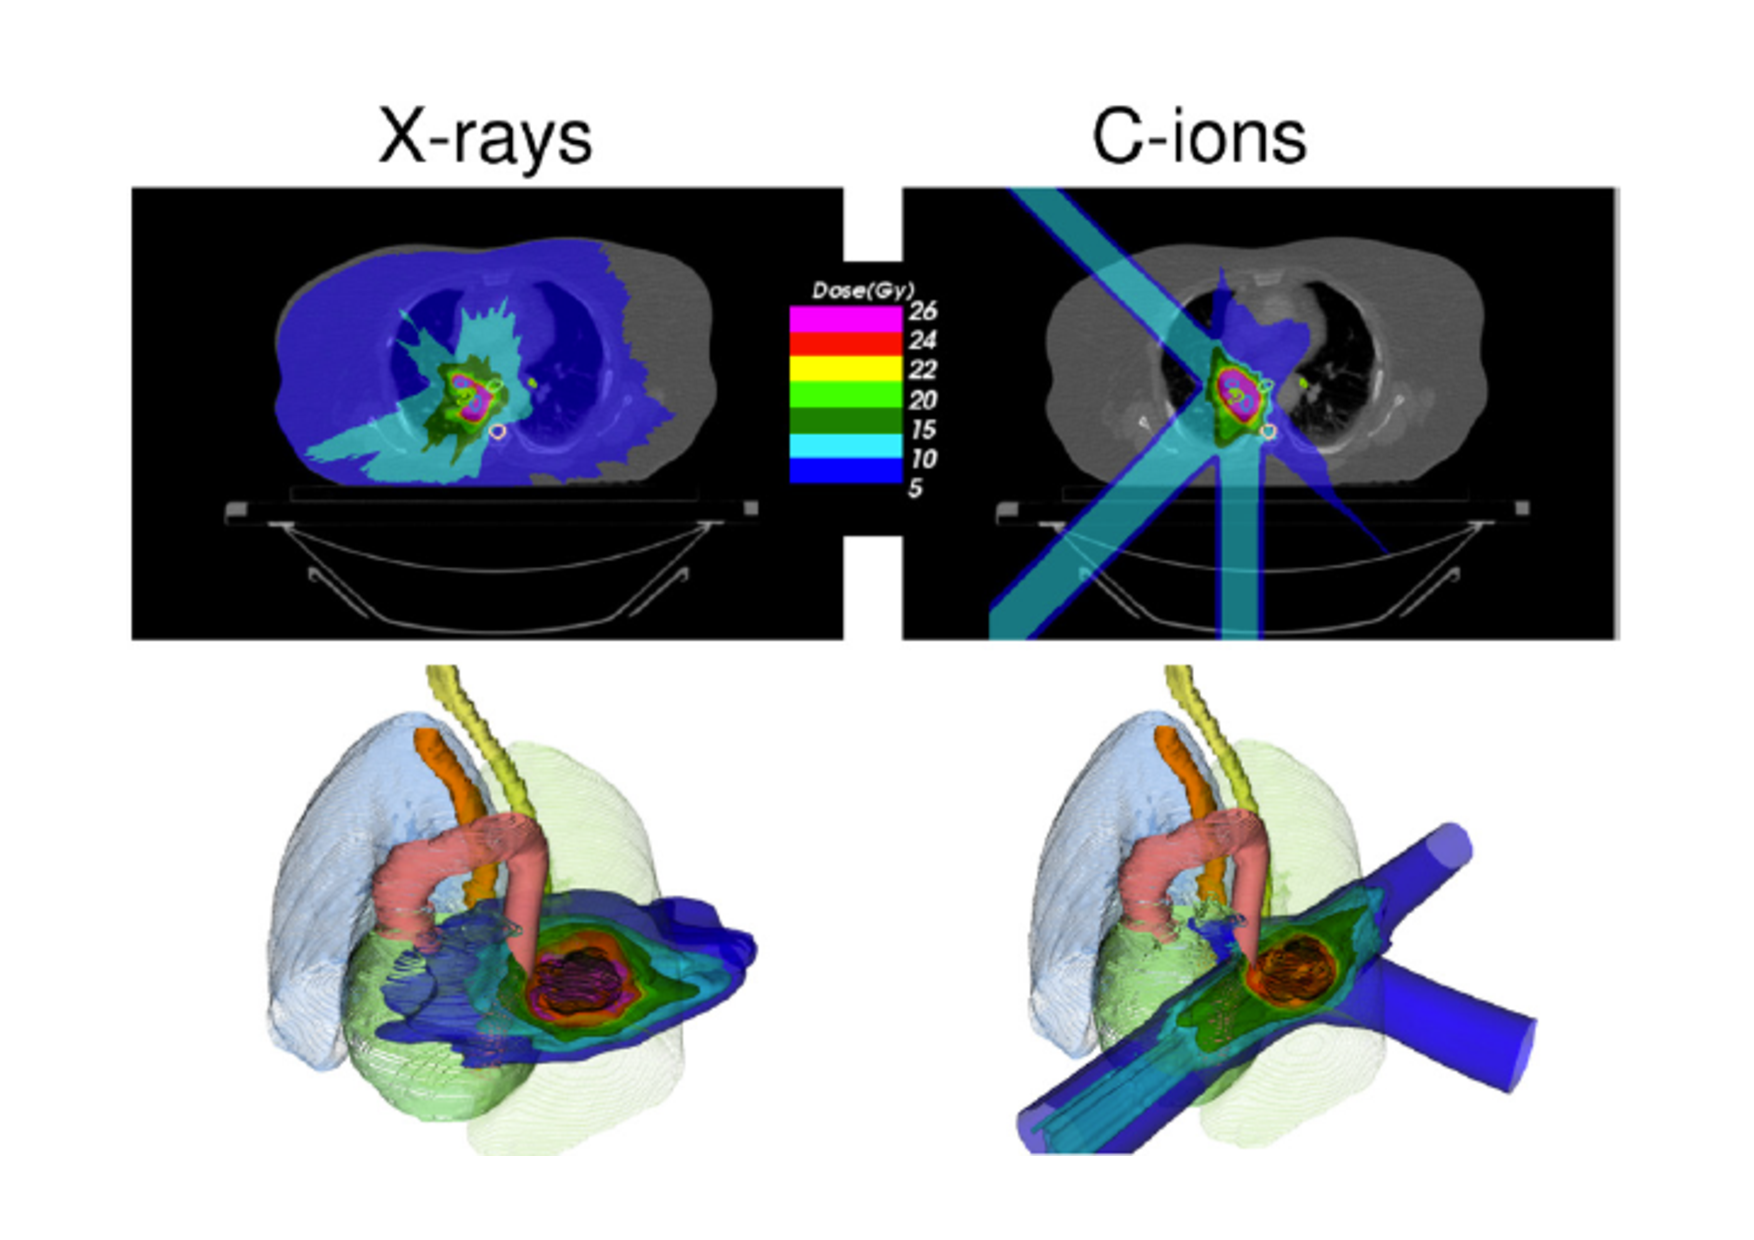
\includegraphics[width=0.8\textwidth]{03_GraphicFiles/chapter1_Introduction/xRayCions_fields.pdf}
\caption{Treatment planning of lung cancer for the irradiation with x-rays (left) or carbon ions (right) (in~\cite{Durante2016}).}
\label{chap1::fig::XraysCionsFields}
\end{figure} 

\begin{figure}[!htbp]
\centering
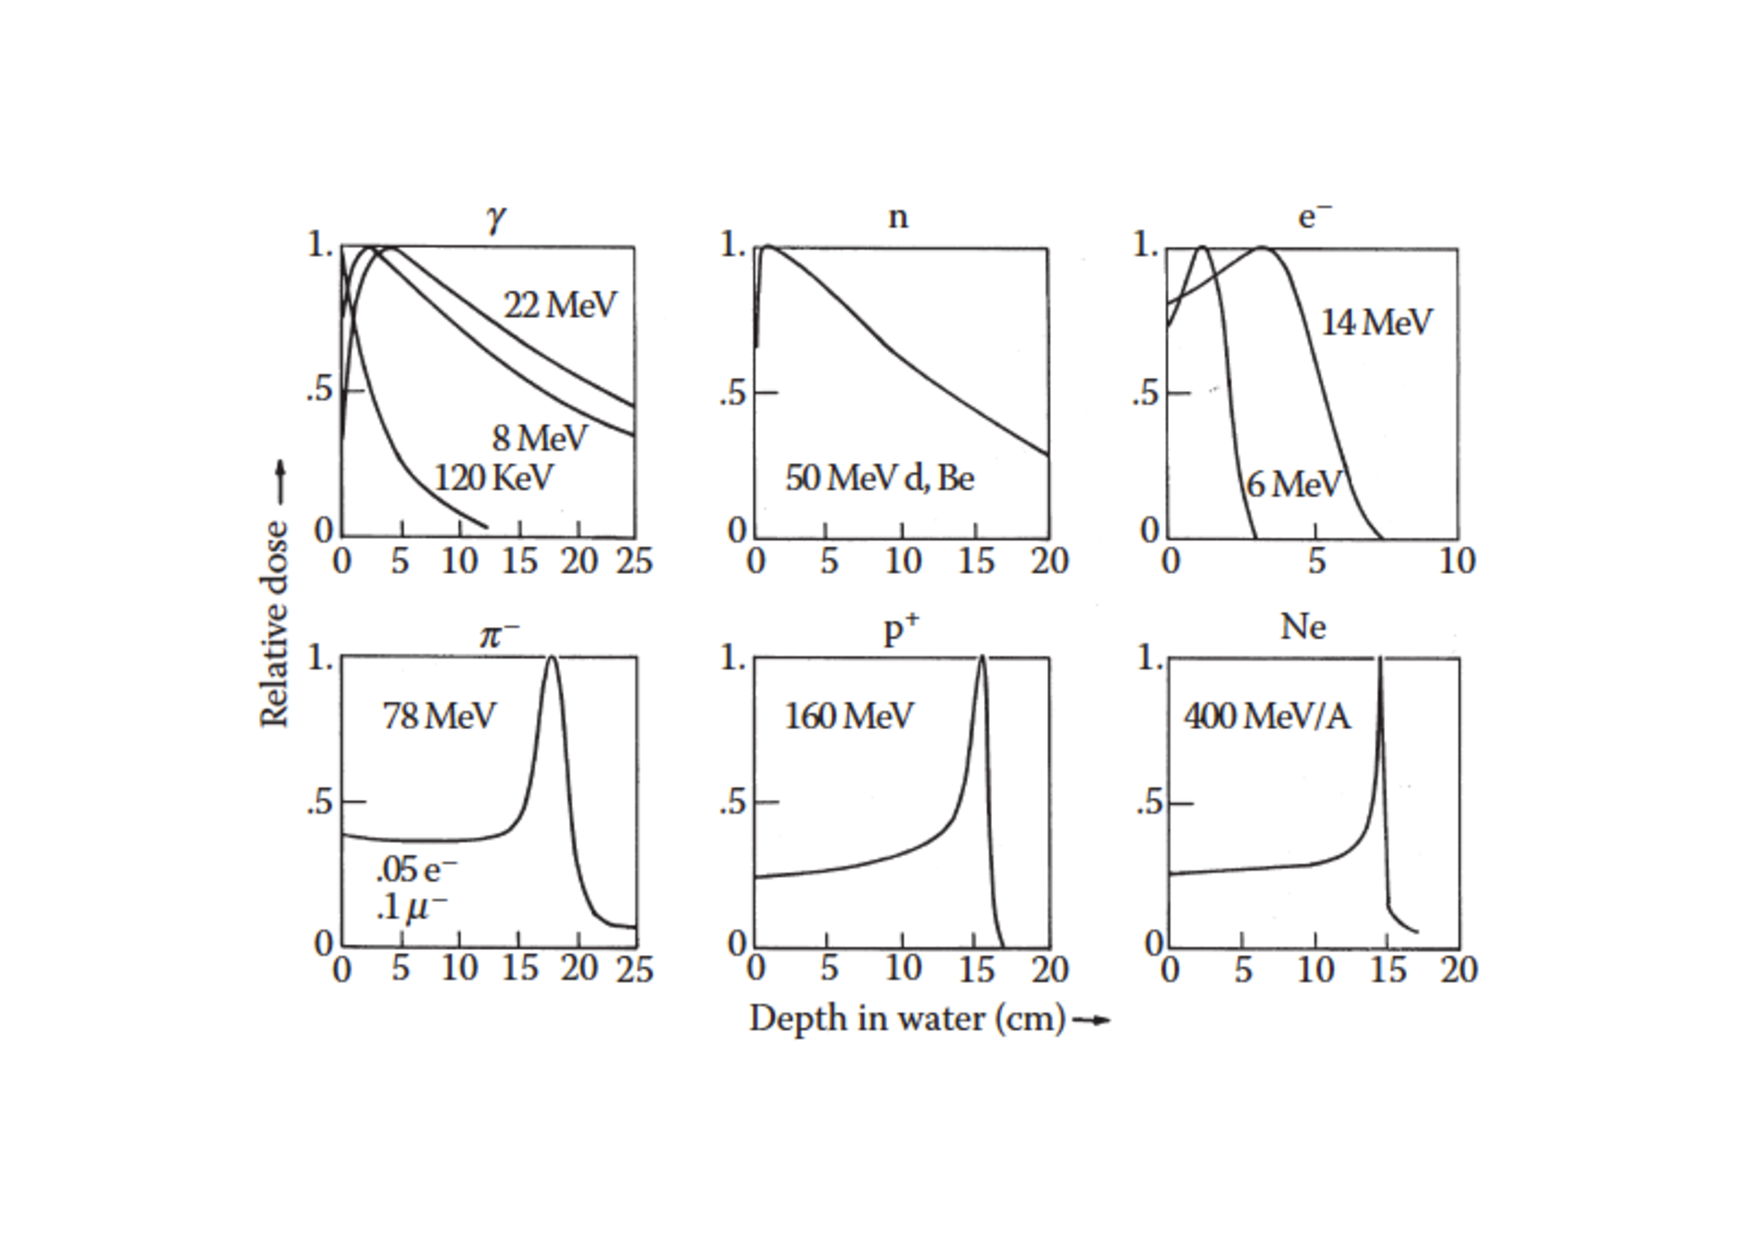
\includegraphics[width=0.8\textwidth , trim={0.5cm 0.5cm 0.5cm 0.5cm}, clip=true]{03_GraphicFiles/chapter1_Introduction/depth_doseProf_multipleIMG.pdf}
\caption{Relative dose as a function of the particle depth in water for different particle species. For photons, the reported energy in MeV corresponds to MV linac-accelerated electron induced bremmstrahlung. In~\cite{PaganettiBook2012}.}
\label{chap1::fig::Depth-doseProf}
\end{figure} 

\subsubsection{Charged particle interactions in matter}\label{chap1::subsubsec::ionInteractions}

The nuclear charged particle interactions in matter can be described by three main mechanisms: \gls{em} inelastic interaction with the atomic electrons, \gls{em} elastic interactions with the atomic nuclei, and nuclear reactions. In addition to the listed interactions, also Bremsstrahlung is theoretically possible, but its effect is negligible at ion energies of clinical interest. 
The \gls{em} inelastic interactions with atomic electrons cause an energy loss which is generally approximated with a \gls{csda} for simplicity, assuming a mono-dimensional quasi-linear ion path and an average, continuous energy loss rate. The mass difference between electrons and ions (as an example, the proton mass is 1832 times greater than that of an electron), justifies the quasi-linear approximation, while the significant cross-section for small energy transfer allows one to consider a continuous decelerating force. The elastic repulsion caused by an atomic nucleus is able to deflect the projectile ion, with an angle which depends on the target-projectile relative mass. The inelastic nuclear reactions are less frequent, but reduce the intensity of the primary beam (the primary particle is destroyed or deflected at large angle), and cause the emission of secondary nuclear fragments. A schematic view of the three main interaction mechanisms described is given in \figurename~\ref{chap1::fig::protInteractions} for the example case of protons, while in the following the effects of these interactions are detailed.   

\begin{figure}[!htbp]
\centering
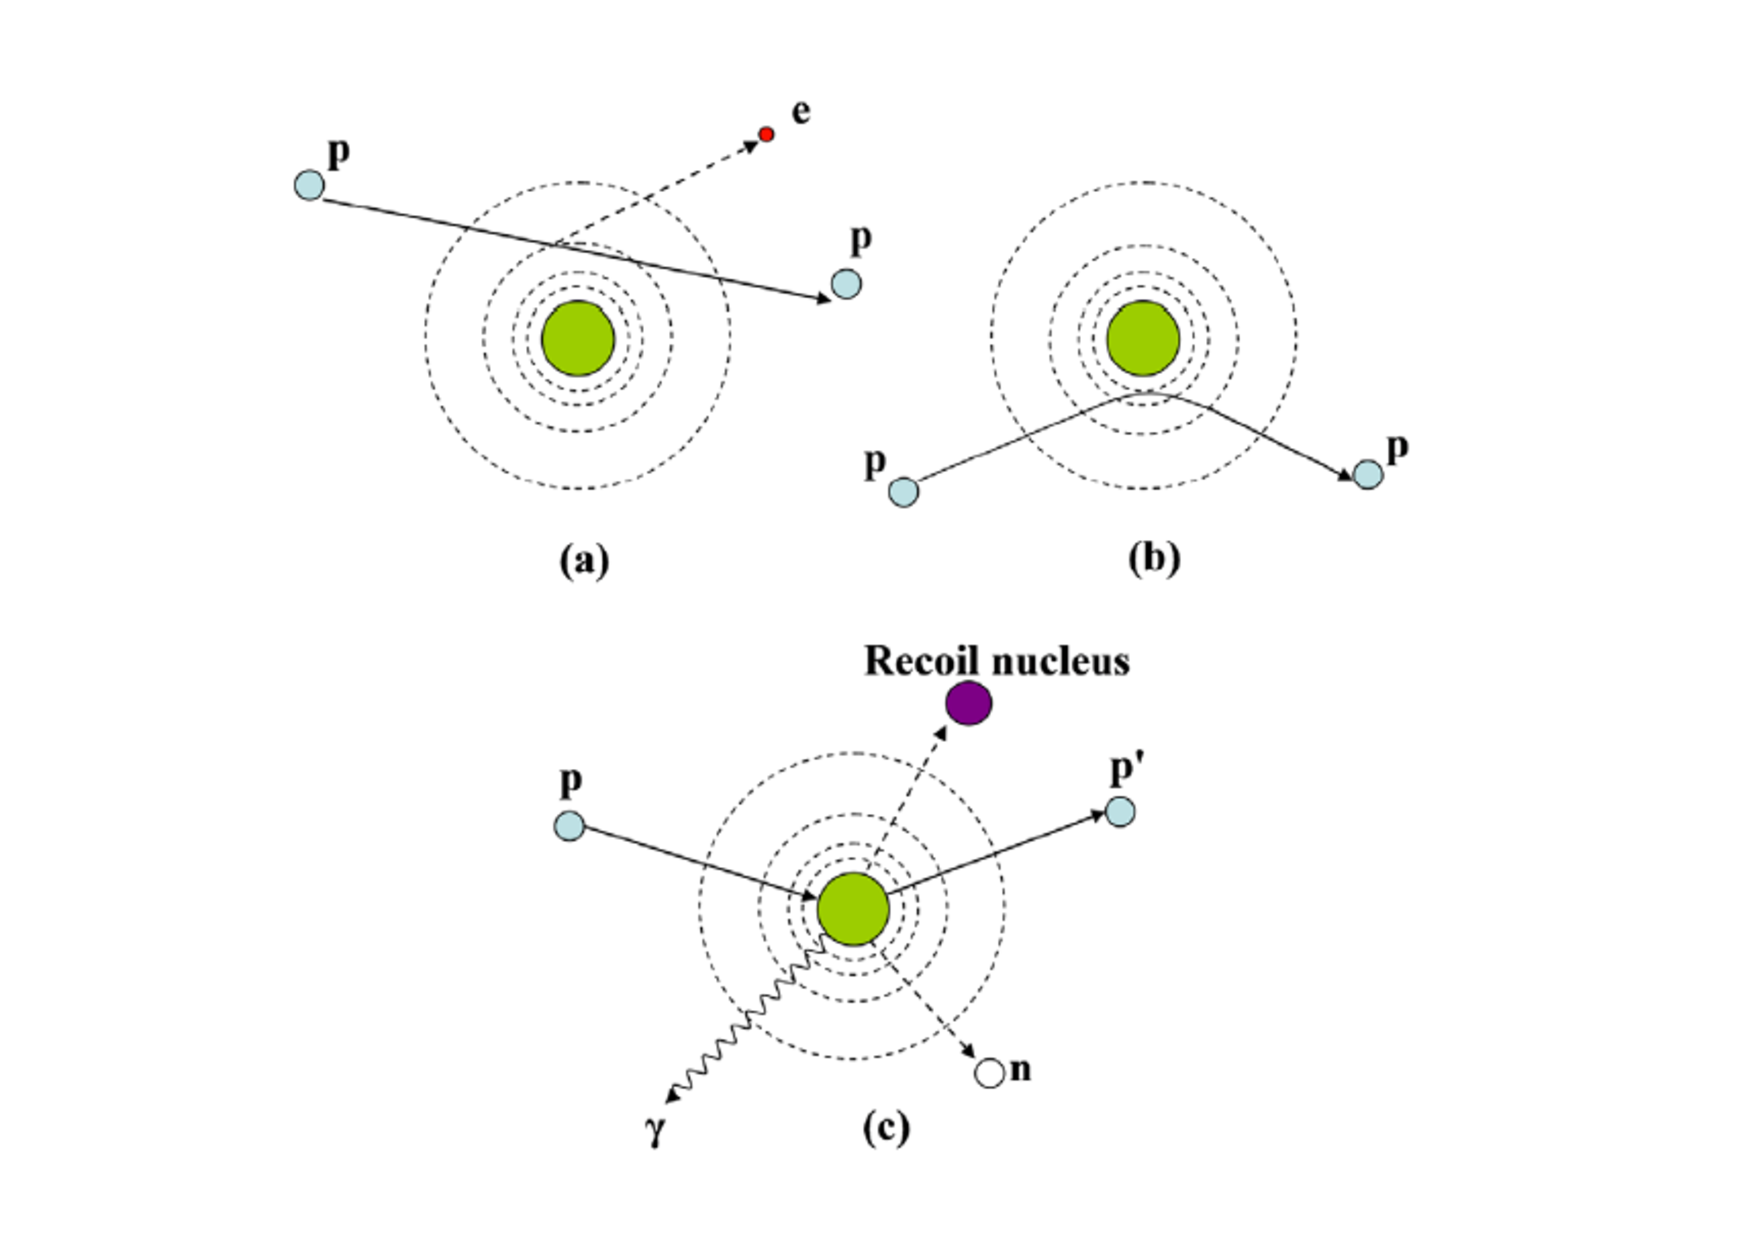
\includegraphics[width=0.8\textwidth]{03_GraphicFiles/chapter1_Introduction/protonInteractions.pdf}
\caption{Schematic view of an example of the three main interactions mechanics of protons in matter: Coulomb interaction with atomic electrons (a), Coulomb interactions with atomic nucleus (b), nuclear reactions(c). In~\cite{Newhauser2015}.}
\label{chap1::fig::protInteractions}
\end{figure} 

At the primary particle velocities of clinical interest,  \myMarginnote{\gls{em} \\ interactions with \\ target atomic electrons} the ion energy loss rate is dominated by inelastic collisions with the target atomic electrons and is well described by the formula attributed to Bethe~\parencite{Bethe1930} and Bloch~\parencite{Bloch1933}, often referred as Bethe-Bloch formula, reported in equation~\ref{chap1::eq::bethe-bloch} in its form independent of the mass density. This expression is also known as mass stopping power.

\begin{equation}
\frac{S}{\rho} = -\frac{\mathrm{d}E}{\rho \mathrm{d}x} = 4\pi N_{A}r^{2}_{e}m_{e}c^{2}\frac{z^{2}}{\beta^{2}}\frac{Z}{A}\bigg[\ln{\frac{2m_{e}c^{2}\beta^{2}\gamma^{2}}{I}}-\beta^{2}-\frac{\delta}{2}-\frac{C}{Z}\bigg]
\label{chap1::eq::bethe-bloch}
\end{equation}

where $N_{A}$ is the Avogadro's number (6.022 $\times$10$^{23}$mol$^{-1}$), $r_{e}$ is the classical electron radius expressed in equation~\ref{chap1::eq::electronRad} with $\epsilon_{0}$ = 8.854 $\times$ 10$^{-12}$~F/m the permittivity of the vacuum, $m_{e}c^{2}$ = 511~keV the mass energy of the electron, $e$ = 1.6 $\times$ 10$^{-19}$~C the electron charge and $c$ the speed of light,  

\begin{equation}
r_{e} = \frac{1}{4\pi\epsilon_{0}}\frac{e^2}{m_{e}c^{2}} = \mathrm{2.181\times10^{-15} m}
\label{chap1::eq::electronRad}
\end{equation}

$z$ is the charge of the projectile, $Z$ and $A$ are the atomic number and mass of the target material, respectively, $\beta = v/c$ is the projectile velocity, $\gamma = (1-\beta^{2})^{-1/2}$, $I$ is the mean excitation potential of the target material. The last two terms represent corrections for high energies ($\delta$ density effect correction term) and low energies ($C$ shell correction term) incident ions. By observing equation~\ref{chap1::eq::bethe-bloch}, it clearly emerges how the energy loss rate is proportional to the square of charge and inverse velocity of the projectile. The target material composition also plays a major role. As the logarithmic term varies slowly with the target properties, and since Z/A is also almost constant, it turns that the linear energy loss rate is proportional to the electron density, and thus to the atomic density (to be noticed, for clinical applications, that the density in a patient can vary by almost three orders of magnitude, ranging from the air cavity in the lungs to the most dense bones). 
As already mentioned, the energy loss increases for decreasing ion energy due to the $1/\beta^{2}$ dependence at high velocities (when the projectile velocity is much larger than its orbital electron velocities, and therefore remains fully stripped), and the maximum energy-loss rate, corresponding to the Bragg peak depth, is reached at the projectile velocity expresses as

\begin{equation}
v_p = z^{2/3}v_{0}
\label{chap1::eq::maxEloss}
\end{equation}

where $v_{0} = e^2/\hslash$ is the Bohr velocity ($\beta$ = 1/137). For velocity values below $v_p$, corresponding to the average orbital velocity in the Thomas-Fermi atomic model, the ion captures electrons and its charge decreases, as well as the stopping force. However, the residual range is small (a few tens micrometers), and therefore the Bragg peak is assimilated to the end of the ion path. Note that, at very small velocities, atomic elastic collisions become important in the slowing down process. 

The energy loss rate equation directly leads \myMarginnote{Ion range} to the definition of the ion beam range in matter (if we neglect nuclear interactions which cause a modification of the projectile nature), which is the integral over the incident energy of the energy loss per track unit, reported in equation~\ref{chap1::eq::rangeIntegral}. This formulation assumes a 1D ion trajectory with negligible lateral scattering (mentioned above and discussed below) and uses the \gls{csda}. 

\begin{equation}
R(E) = \int_{0}^{E}(\frac{\mathrm{d}E'}{\mathrm{d}x})^{-1}\mathrm{d}E' 
\label{chap1::eq::rangeIntegral}
\end{equation}

where E is the ion beam incident energy. To be noticed that the range is not a deterministic value, but it is intended as an average value and defined for the whole beam, not for single incident particles, which are affected by statistical fluctuations in the energy loss, leading to the so-called \enquote{range straggling} (described by different theoretical models, such as the ones in~\cite{Bohr1915, Landau1944, Vavilov1957}, and detailed below). The integration of the Bethe-Bloch is often a hard task, but, as realized by Bragg and Kleeman~\parencite{Bragg1905}, the range dependence on the incident particle energy can be practically expressed with an analytic approach as the power law in equation~\ref{chap1::eq::rangePowerLaw}. This approximation directly derives from studies on alpha particles which anticipated the formulation of equation~\ref{chap1::eq::bethe-bloch}.

\begin{equation}
R(E) = \alpha E^{p}
\label{chap1::eq::rangePowerLaw}
\end{equation}

where E is again the ion beam initial energy, the constant $\alpha$ depends on the target material and the constant $p$ is related to the projectile energy (or velocity). The proton range can be easily scaled to other ions at the same energy per nucleon in the same material with a factor $M/z^{2}$, where $M$ is the ion mass. The range of ions with the same specific energy scales from water to other homogeneous material with a factor of $A/Z^{2}$.
%An empirical expression has been derived to scale the proton calculated range to heavier ions at the same energy per nucleon in the same material: it is reported in equation~\ref{chap1::eq::ScaleRange}.

%\begin{equation}
%\frac{R_{2}}{R_{1}} = \frac{M_{2}}{M_{1}}\frac{z_{1}^{2}}{z_{2}^{2}}
%\label{chap1::eq::ScaleRange}
%\end{equation}

%with M and z the ion mass and charge, respectively. Equivalently, for the same particle in different material, the scaling formula is reported in equation~\ref{chap1::eq::ScaleRangeMat}.

%\begin{equation}
%\frac{R_{2}}{R_{1}} = \frac{\rho_{2}}{\rho_{1}}\frac{\sqrt{A_{1}}}{\sqrt{A_{2}}}
%\label{chap1::eq::ScaleRangeMat}
%\end{equation}
 
% with $\rho$ and $A$ density and atomic mass of the target material, respectively.
 
The ion range predicted by equations~\ref{chap1::eq::rangeIntegral} or~\ref{chap1::eq::rangePowerLaw} \myMarginnote{Range straggling} is an average value, calculated by considering a smooth and continuous energy loss process and neglecting the individual ion behavior. The actual range suffers from statistical fluctuations in the projectile energy loss that broaden the Bragg peak, in the so-called \enquote{range straggling}. In general, the longitudinal beam straggling can be described by an asymmetric distribution~\parencite{Vavilov1957}, which is approximated to a Gaussian in the limit of many collisions, leading to the expression of the relative straggling in equation~\ref{chap1::eq::relStragg}:
 
 \begin{equation}
\frac{\sigma_{R}}{R} = (M^{-\frac{1}{2}})\phi\frac{E}{Mc^{2}}
\label{chap1::eq::relStragg}
\end{equation}

The ratio of the straggling width $\sigma_{R}$ and mean range $R$ is then all the more reduced as the ion mass ($M$) increases, with $\phi$ a slowly varying function which depends on the target material~\parencite{Rossi1952} and E the ion energy. According to equation~\ref{chap1::eq::relStragg}, it is interesting to notice how the relative straggling for carbon ions is about 3.5 times smaller with respect to protons (e.g. 7~mm and 25~mm at 18~cm of average range for carbon ions and protons, respectively - see~\cite{Durante2016}). In addition to energy loss fluctuations, range straggling contributions also come from the beam initial energy distribution: the actual beam is not perfectly mono-energetic, and the energy distribution width is determined by the accelerator and the beam optics elements. This contribution has to be added (quadratic sum) to the range straggling estimate. Figures~\ref{chap1::fig::TailBragg_p} and~\ref{chap1::fig::TailBragg} show the depth-dose profiles of proton and carbon ion mono-energetic beams, respectively, at different energies in water. The effect of range straggling is clearly visible in the broadening of the Bragg peak, which is more significant for protons with respect to carbon ions, and increases for increasing range in matter.  

In addition to the energy loss process considered till here,  \myMarginnote{\gls{em} \\ interactions with \\ target nuclei} which shapes the beam in the longitudinal direction (range variations), the actual delivered dose also depends on the lateral beam profile, which derives from the size and angular divergence of the incident beam and is mainly governed, at the target level, by elastic Coulomb scattering with atomic nuclei and by secondary particles produced by nuclear fragmentation. 
In case an ion passes close to a target atomic nucleus, it is elastically scattered by the repulsive electromagnetic force: the projectile loses a negligible amount of energy, so that this kind of interaction can be neglected when calculating the energy loss rate described above, but the change in its trajectory must be estimated for range and dose predictions. %The \gls{mcs} is determined by elastic electromagnetic interactions of the beam ions with the target nuclei, causing considerable deflections in the single ion trajectory which mainly affect the lateral beam profile causing a spread. 
Starting from the single scattering model by Rutherford~\parencite{Rutherford1911}, and moving to the calculation of the statistical distribution function for the scattering angle at a certain penetration depth given by~\cite{Bothe1921}, a complete theory allowing for the calculation of the scattering angle probability in case of \gls{mcs} has been proposed by Moli\`{e}re~\parencite{Moliere1948} (confirmed to provide good predictions thanks to a large set of proton beam spread data - see~\cite{Gottschalk1993}). More practical formulas were then derived afterwards (see~\cite{Lewis1950, Highland1975, Gottschalk2010}). The Moli\`{e}re formulation has been then simplified for analytic calculations towards a Gaussian approximation. The Gaussian standard deviation ($\sigma_{\theta}$) expression in equation~\ref{chap1::eq::latSpread} is given by the characteristics \gls{mcs} angle $\theta$~\parencite{Highland1975}

\begin{equation}
\sigma_{\theta} = \frac{14.1 \mathrm{MeV}}{\beta p c}Z_{p}\sqrt{\frac{L}{L_\mathrm{rad}}}\big[1+0.038 \ln\big(\frac{L}{L_{\mathrm{rad}}}\big) \big]
\label{chap1::eq::latSpread}
\end{equation}

where $\beta$, $p$ and $Z_{p}$ are respectively the projectile velocity, momentum and charge, $c$ is the speed of light,  $L$ is the material thickness and $L_{\mathrm{rad}}$ is the radiation length (reported for common materials in~\cite{Tsai1974}). 
Even if the Gaussian approach is not always accurate to describe the lateral beam spread (mainly at large angles), the Moli\`{e}re \gls{mcs} description allows to retrieve the main parameters contributing to this effect: in particular, heavier particles have narrower lateral beam spread, and the scattering effect increases at increasing ion range (but is inversely proportional to the beam energy) and for high-Z materials. A more precise model of the lateral beam spread should involve nuclear reactions and the produced secondary particles, but an analytic approach is difficult and Monte Carlo based calculations are necessary, but still time consuming. The empirical parameterizations are still strongly based on experimental data: as an example, measurements of the lateral beam spread in a water column for different beam energies (ranges) are reported in~\cite{Pedroni2005}. In~\figurename~\ref{chap1::fig::latSpread} the lateral spread of different ions in water is plotted as a function of range for various beam energies (A) and as a function of beam energy (B) after 15~cm range in water.

\begin{figure}[!htbp]
\centering
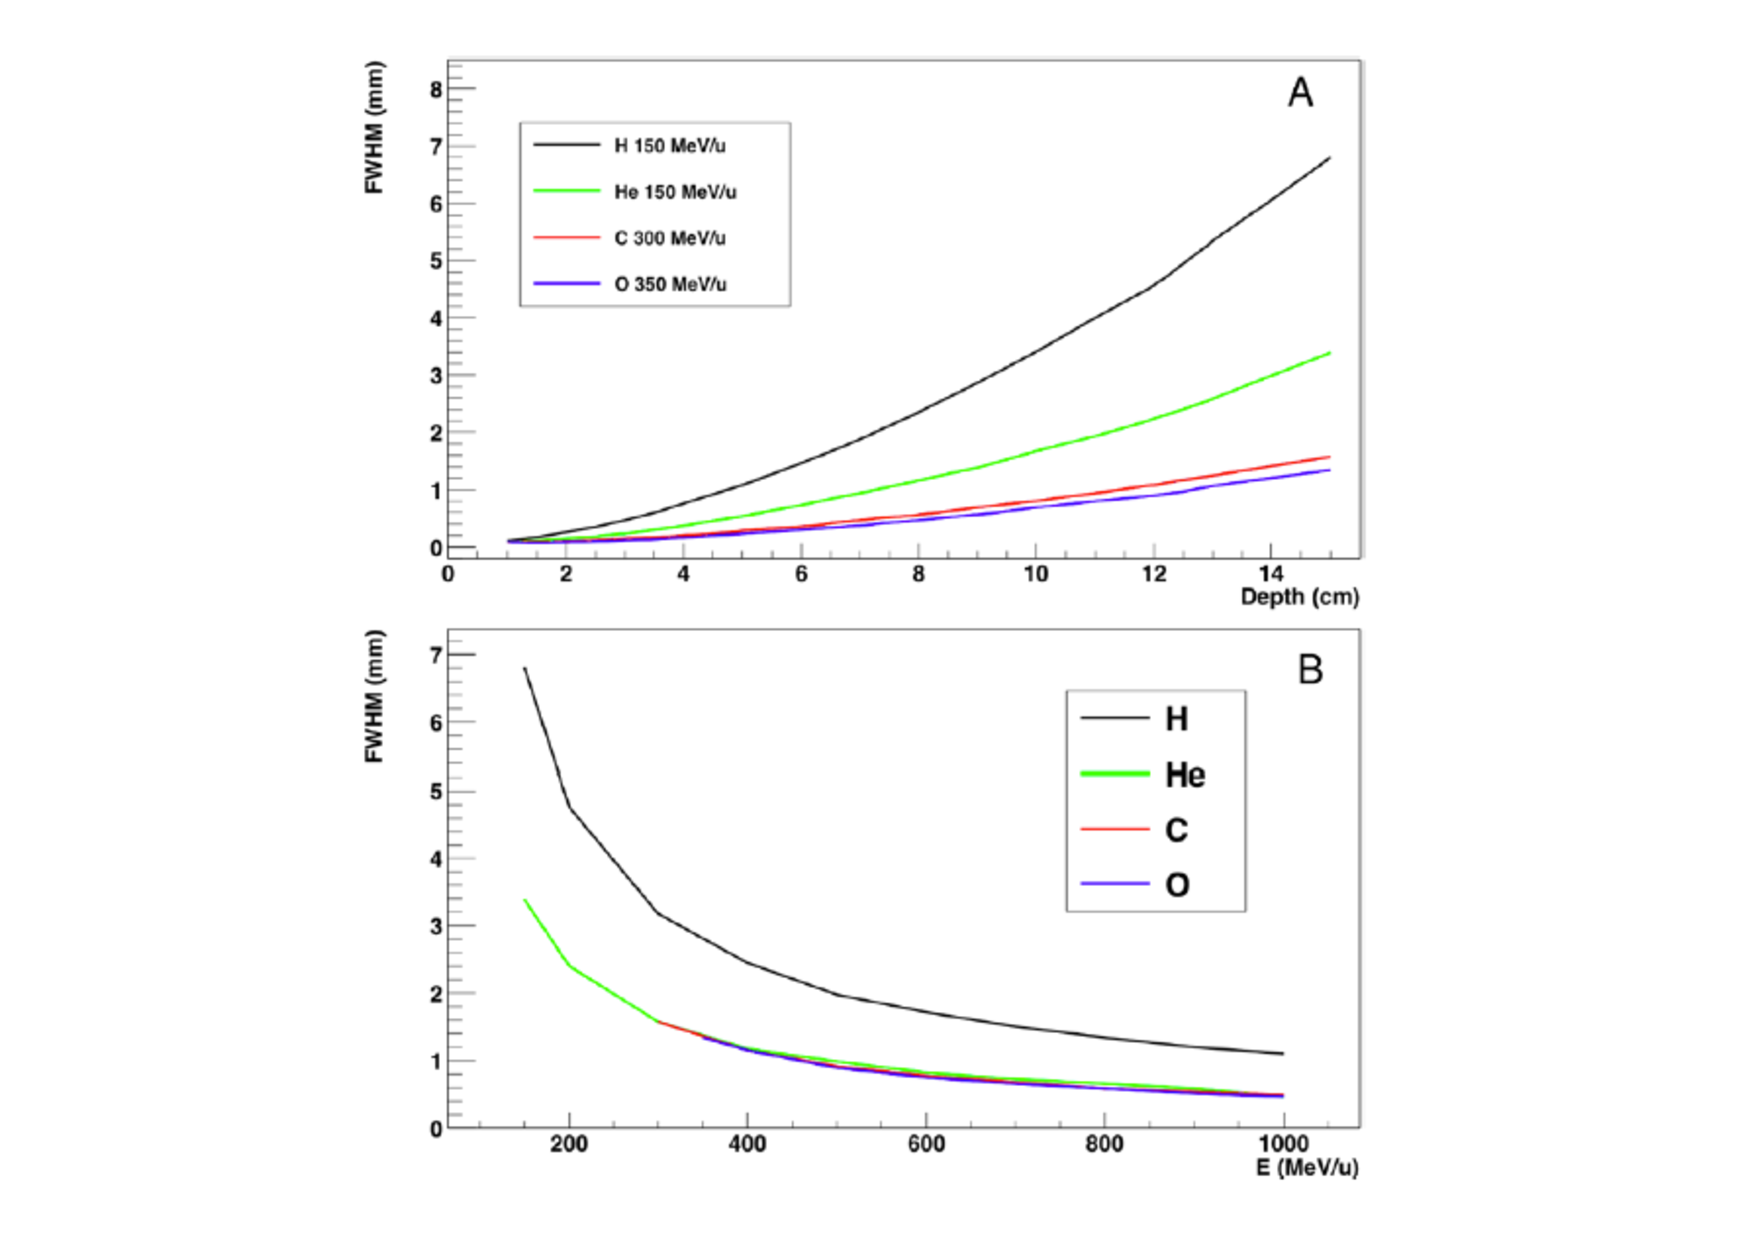
\includegraphics[width=0.8\textwidth]{03_GraphicFiles/chapter1_Introduction/lateralSpread.pdf}
\caption{Lateral spread of different ions in water obtained with Geant4 Monte Carlo simulations. The \gls{fwhm} of the beam spot distribution is presented as a function of depth in water (A) for beams at different energies and as a function of beam energy (B) after 15~cm range in water. In~\cite{Durante2016}.}
\label{chap1::fig::latSpread}
\end{figure}   

In addition to the electromagnetic interactions with electrons and nuclei \myMarginnote{Nuclear reactions}  which mainly govern the stopping process, primary ions impinging on a target also undergo nuclear reactions with the target nuclei which may cause the disintegration of the projectile and the target nucleus or a partial fragmentation. In general, nuclear reactions induce modifications in the beam composition and cause variations in the longitudinal and lateral beam structure which must be taken into account for the delivered physical and biological dose estimate. Moreover, this kind of reactions leads to the production of secondary particles, such as secondary protons, neutrons, hydrogen and helium isotopes and other ions (mainly with heavy ion irradiation), and gammas.
In the high velocity regime (when the relative velocity in the nuclei center of mass is much larger than the nucleon Fermi velocity), the nuclear interactions occurring between projectile ions and target nuclei can be described by a two-step process. At the \enquote{collision} stage, depending on the distance between projectile and target centers (impact parameter $b$), a variable number of nucleons is involved in the interaction and composes the reaction zone generally defined as \enquote{fireball}. The so-called \enquote{spectator} nucleons are almost not affected and create projectile-like and target-like fragments (\enquote{fragmentation} process), often in excited states. After the collision, the excited fireball and fragments decay through the emission of secondary light particles, in the so-called \enquote{de-excitation} process, and the lighter fragments continue their path through the target. A schematic view of a typical nuclear reaction is given in \figurename~\ref{chap1::fig::nuclReac}. 
Several models have been proposed to describe the nuclear interactions in its two steps. The \gls{inc} model has been originally proposed by Serber and Heisenberg~\parencite{Serber1947}, and later implemented in the sixties~\parencite{Bertini1974}, and is used to describe the collision stage. It is based on a series of two-body interactions between the incident particle and the target nucleons, which are considered quasi-free. For each nuclear interaction, the code models the complete outcome, and all produced particles are tracked until they are below a given energy threshold, in a process called \enquote{intra-nuclear cascade}. Other candidates are the \gls{qmd}, which describes each nucleon as a gaussian wave packet, and all nucleons are included in the collision, and the \gls{bme}, which is a sophisticated model describing the thermalization of composite nuclei for low energy projectiles. The de-excitation stage can involve the so-called \enquote{evaporation}~\parencite{Weisskopf1937}, where light fragments are emitted from the excited nuclei, \enquote{fission} of the excited nuclei in two fragments (for high-Z nuclei which can be only found in implants), \enquote{Fermi-breakup} of light nuclei which disassembles in smaller fragments~\parencite{Fermi1950}, gamma emission to dissipate the residual energy. 
The majority of the complete models for nucleus-nucleus reactions includes the previously described ones (often in simplified versions, optimized in order to minimize the calculation time) and is a variant of the so-called \enquote{abrasion-ablation} model~\parencite{Hufner1975}, generally used in therapy transport codes. The abrasion phase describes the collision and the ablation one models the de-excitation stage; to be noticed that the ablation description is generally more adapted to peripheral collisions (high $b$), where the fragments are excited after the collision and decay to the ground state by emitting light particles and gamma rays. 

\begin{figure}[!htbp]
\centering
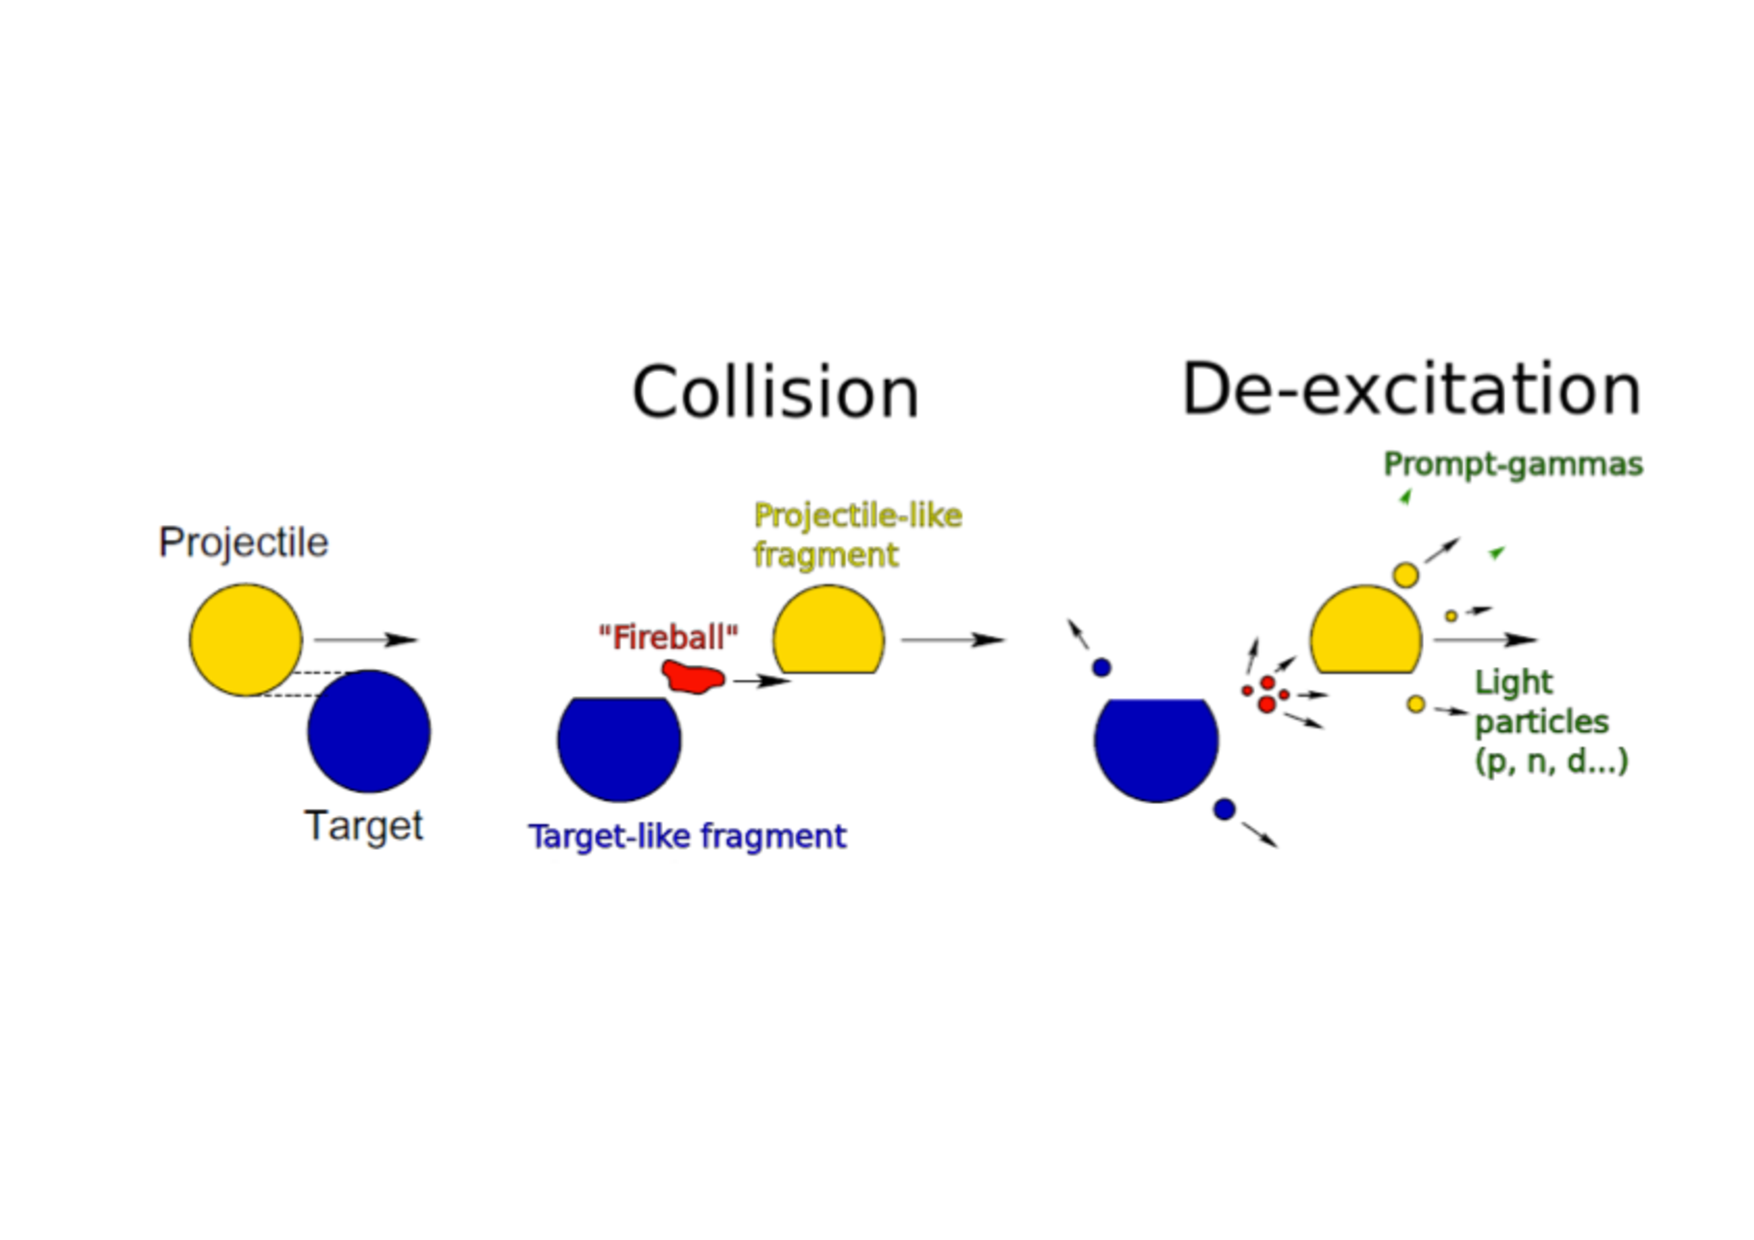
\includegraphics[trim={0 5cm 0 3cm} , clip , width=0.95\textwidth]{03_GraphicFiles/chapter1_Introduction/nuclReactionsScheme.pdf}
\caption{Schematic view of the nuclear reaction between a projectile and a target nucleus. The two steps are defined as \enquote{collision} and \enquote{de-excitation} processes.}
\label{chap1::fig::nuclReac}
\end{figure} 

%, depicted in \figurename~\ref{chap1::fig::abrAbl}.
%\begin{figure}[!htbp]
%\centering
%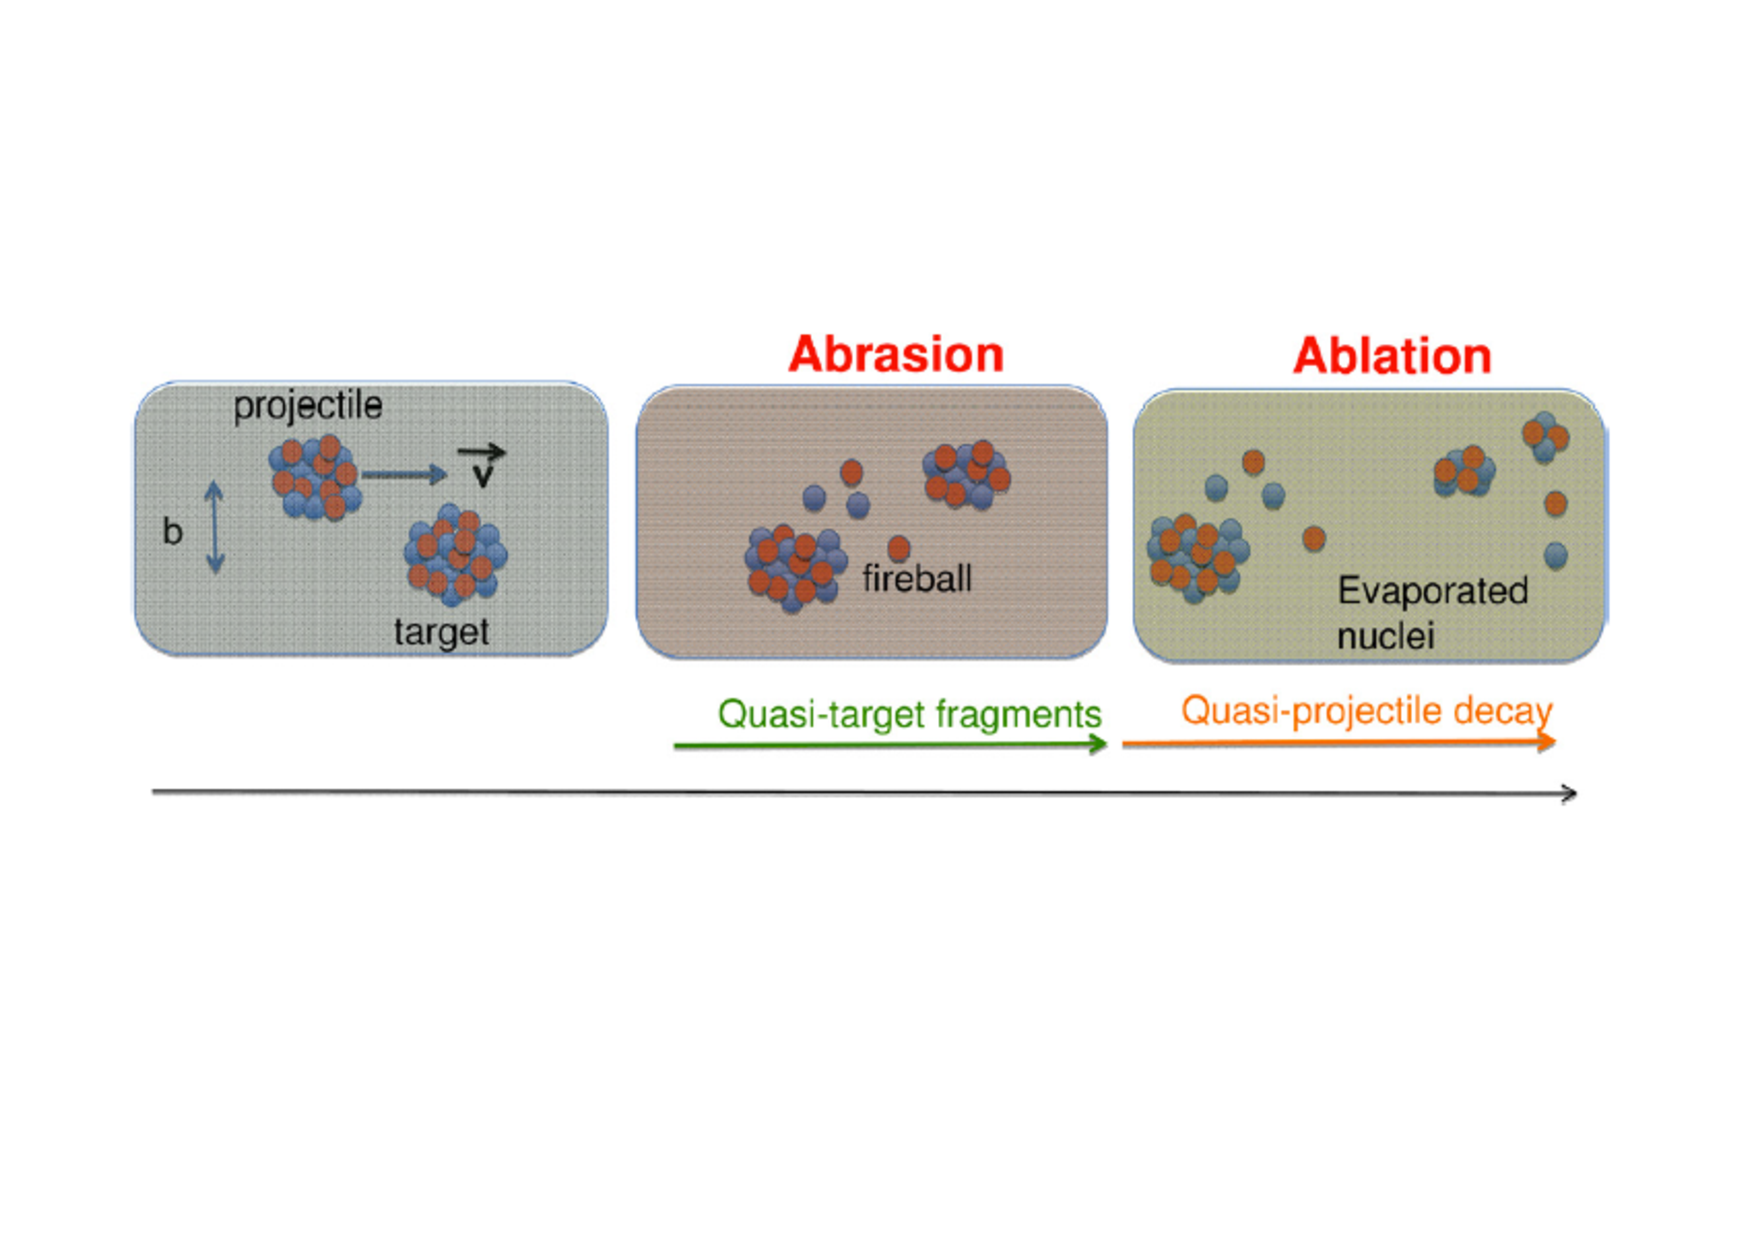
\includegraphics[trim={0 5cm 0 3cm} , clip , width=0.95\textwidth]{03_GraphicFiles/chapter1_Introduction/AbrasionAblation.pdf}
%\caption{Schematic view of the abrasion-ablation model for the description of ion-nucleus interactions (in~\cite{Durante2016}): b is the impact parameter, v is the projectile velocity.}
%%\end{figure} 

Two main effects of fragmentation processes are relevant to ion beam therapy. 
First, the described nuclear reactions cause a loss of primary beam particles; this effect is all the more important for increasing penetration depth. It is clear that peripheral collisions (high $b$) lead to smaller loss of primaries with respect to central collisions (small $b$), where projectile and target are most likely completely destroyed. Figures~\ref{chap1::fig::nuclearReacLoss} and~\ref{chap1::fig::nuclearReacLoss_Cion} (top panel) show the primary particle fluence loss in a proton  and carbon ion beam, respectively, as a function of the depth in water. In the entrance region before the falloff the fluence loss is caused by nuclear reactions, while close to the Bragg peak the fluence falloff is mainly due to stopping of primary particles with zero residual energy. In addition, the range straggling effect is visible. Concerning carbon ion beams, as reported in~\cite{Durante2016}, during a standard treatment only 50\% of the primary ions reach the Bragg peak region for $\sim$20~cm range, while the others undergo fragmentation processes and are lost.
Second, lower-mass and Z fragments result from the nuclear interactions in case of irradiation with ions heavier than protons (with proton beams, only secondary protons and neutrons are produced).
The projectile velocity determines the velocity of the secondary fragments, which can travel with longer ranges with respect to the primaries due to their reduced mass and charge (remember the range scaling factor $M/z^{2}$): this produces a tail in the dose distribution (for ions heavier than protons). The features of this tail have been deeply studied for different primary ions species ($^{10}$B, $^{12}$C, $^{14}$N, $^{16}$O, $^{20}$Ne), and shell-structure effects have been verified with a non-direct relationship between proton number Z and tails extension~\parencite{Schall1996}.  \figurename~\ref{chap1::fig::TailBragg} (and \figurename~\ref{chap1::fig::nuclearReacLoss_Cion}, bottom panel) shows the effects of nuclear reactions on the Bragg curves related to carbon ion beams at different energies stopping in water, measured in a water column~\parencite{Schardt2008}. With increasing primary energy and, consequently, beam penetration depth, the ratio between Bragg peak and entrance plateau dose is reduced by the decreased number of primary ions (this effect is also visible for proton beams in \figurename~\ref{chap1::fig::TailBragg_p}), while the tail after the Bragg peak is wider due to the increased number of lower-Z fragments traveling with longer range. In addition to this, the energy loss stochastic fluctuations are clearly visible in the broadening of the Bragg peak, as already described.  

\begin{figure}
\begin{subfigure}[t]{.49\textwidth}
\hspace{-1cm} 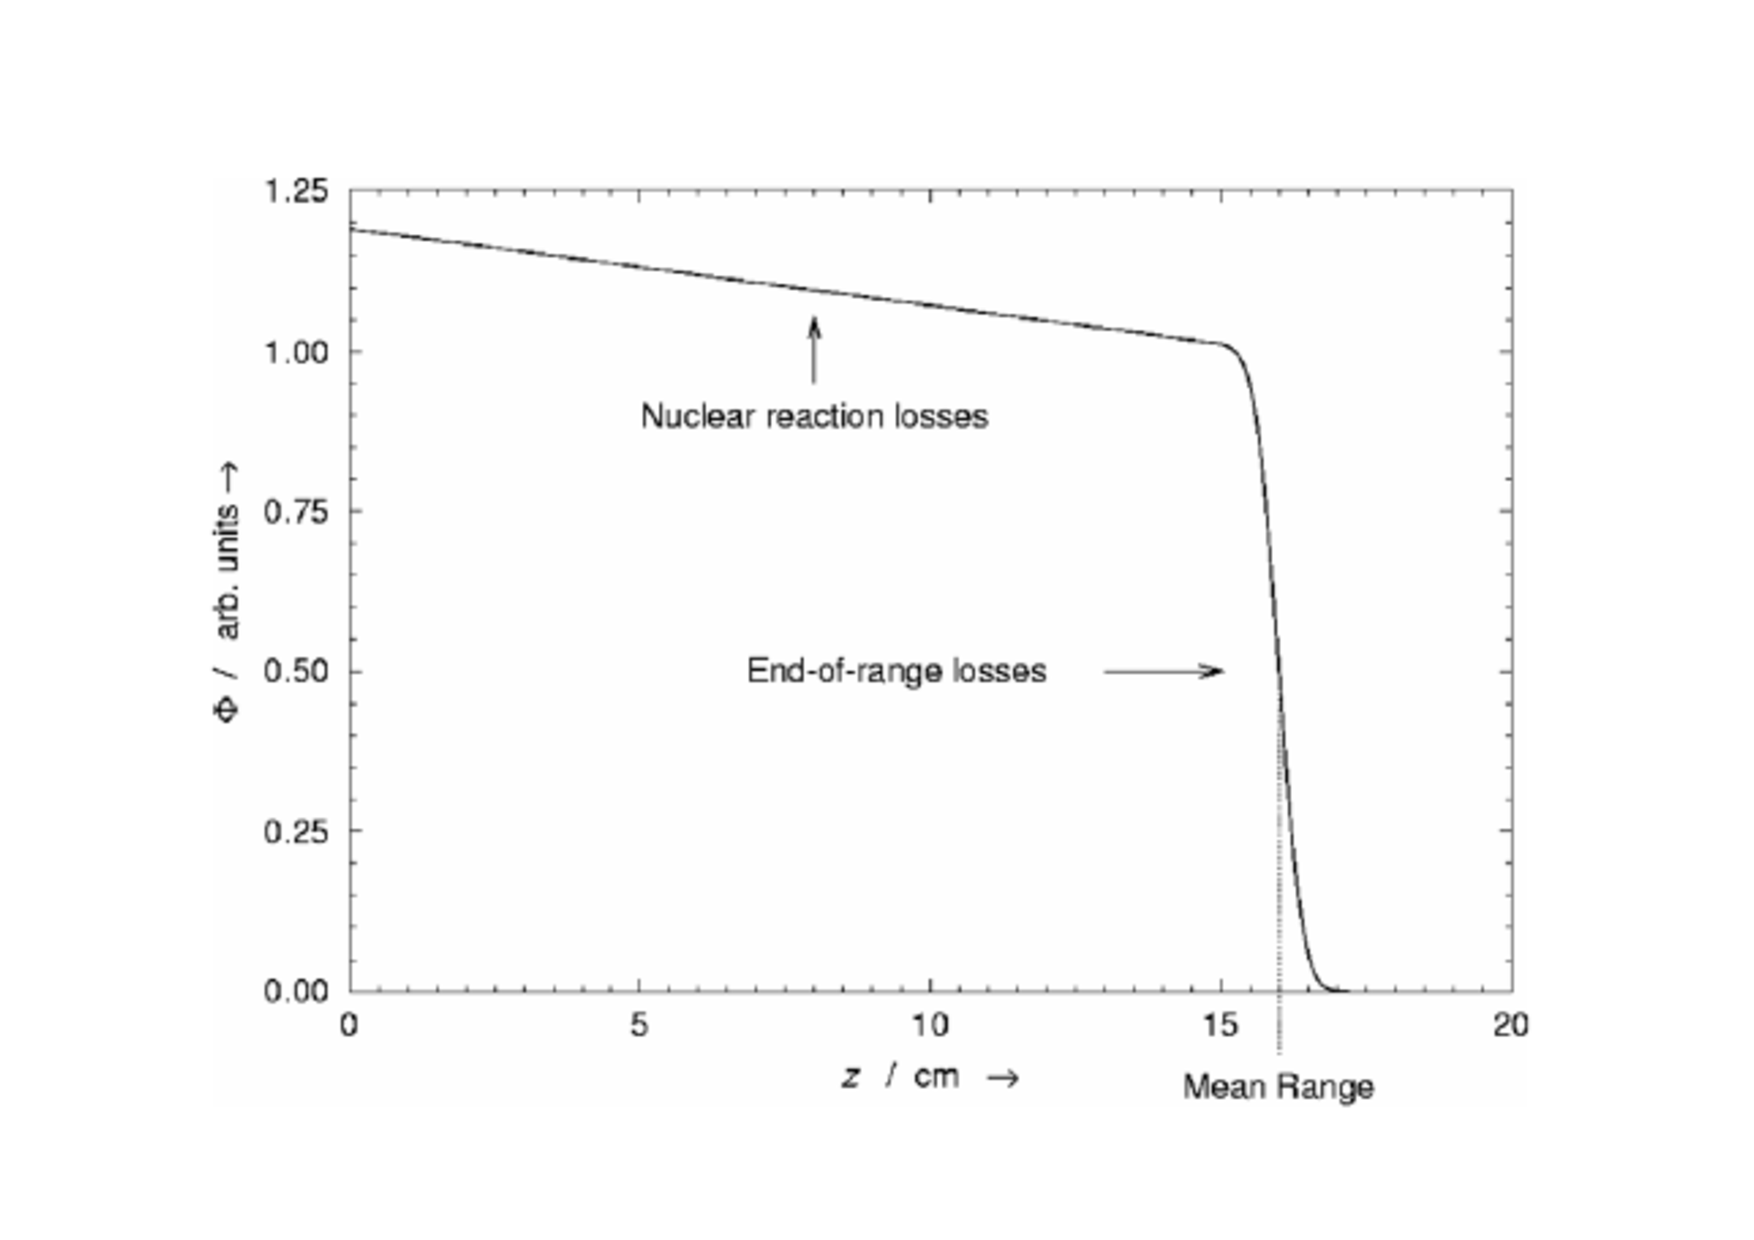
\includegraphics[width=1.2\linewidth]{03_GraphicFiles/chapter1_Introduction/primaryLoss.pdf}
\caption{Primary particle fluence loss in a pro\-ton beam as a function of the depth in water. In~\cite{Newhauser2015}.}
\label{chap1::fig::nuclearReacLoss}
\end{subfigure}
\begin{subfigure}[t]{.49\textwidth}
\hspace{-1cm} 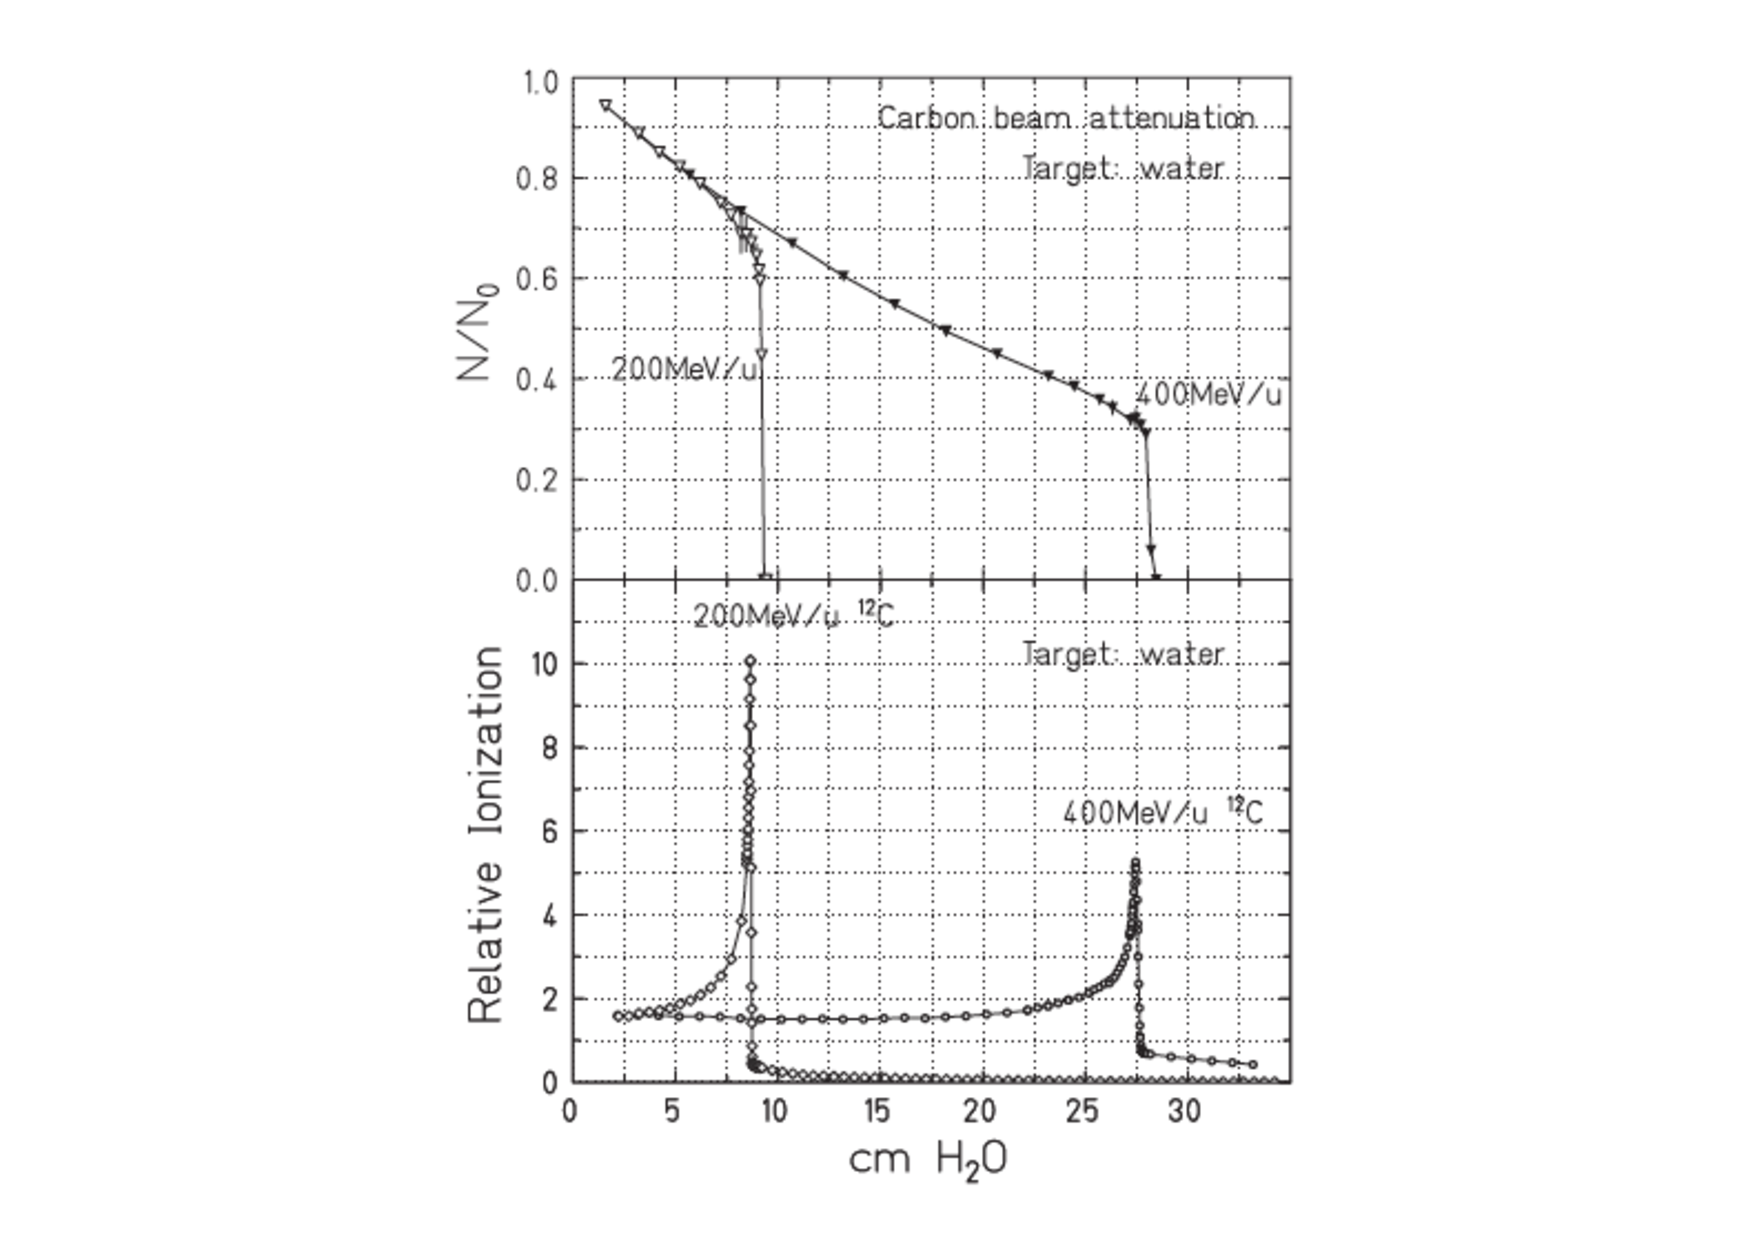
\includegraphics[width=1.2\linewidth, trim={1.5cm 0 1.5cm 0}, clip = true]{03_GraphicFiles/chapter1_Introduction/primaryLoss_Cion.pdf}
\caption{Primary particle fluence loss (top panel) and corresponding Bragg peaks (bottom panel) of carbon ion beams as a function of the depth in water for two initial beam energies. In~\cite{Haettner2006}.}
\label{chap1::fig::nuclearReacLoss_Cion}
\end{subfigure}
\begin{subfigure}[t]{.49\textwidth}
\hspace{-0.6cm} 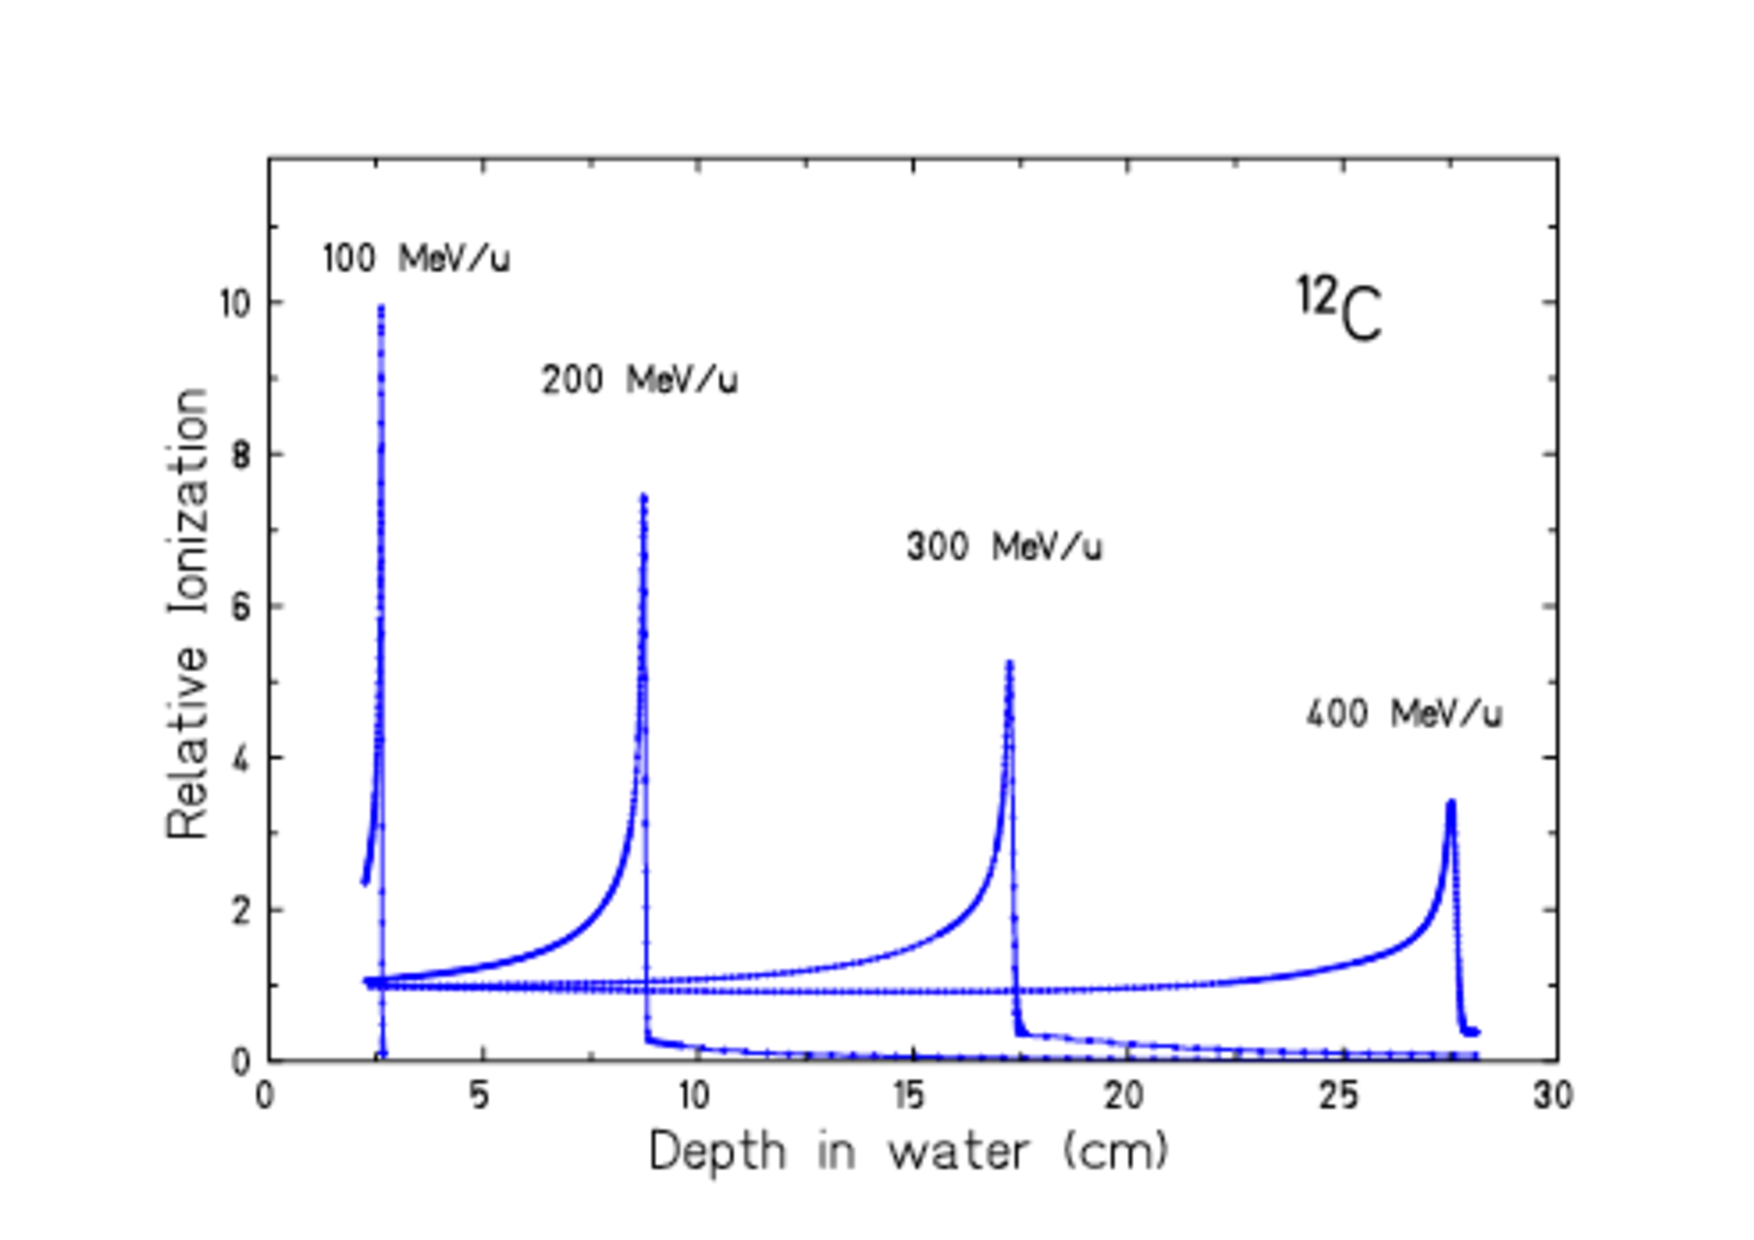
\includegraphics[width=1.1\linewidth, height = 5.9cm]{03_GraphicFiles/chapter1_Introduction/tailBragg.pdf}	
\caption{Integral dose as a function of the depth in water for proton beams at 7 different energies. The crosses represent experimental points, the solid lines are the results of dose model calculations. In~\cite{Pedroni2005}.}
\label{chap1::fig::TailBragg_p}
\end{subfigure}
\begin{subfigure}[t]{.49\textwidth}
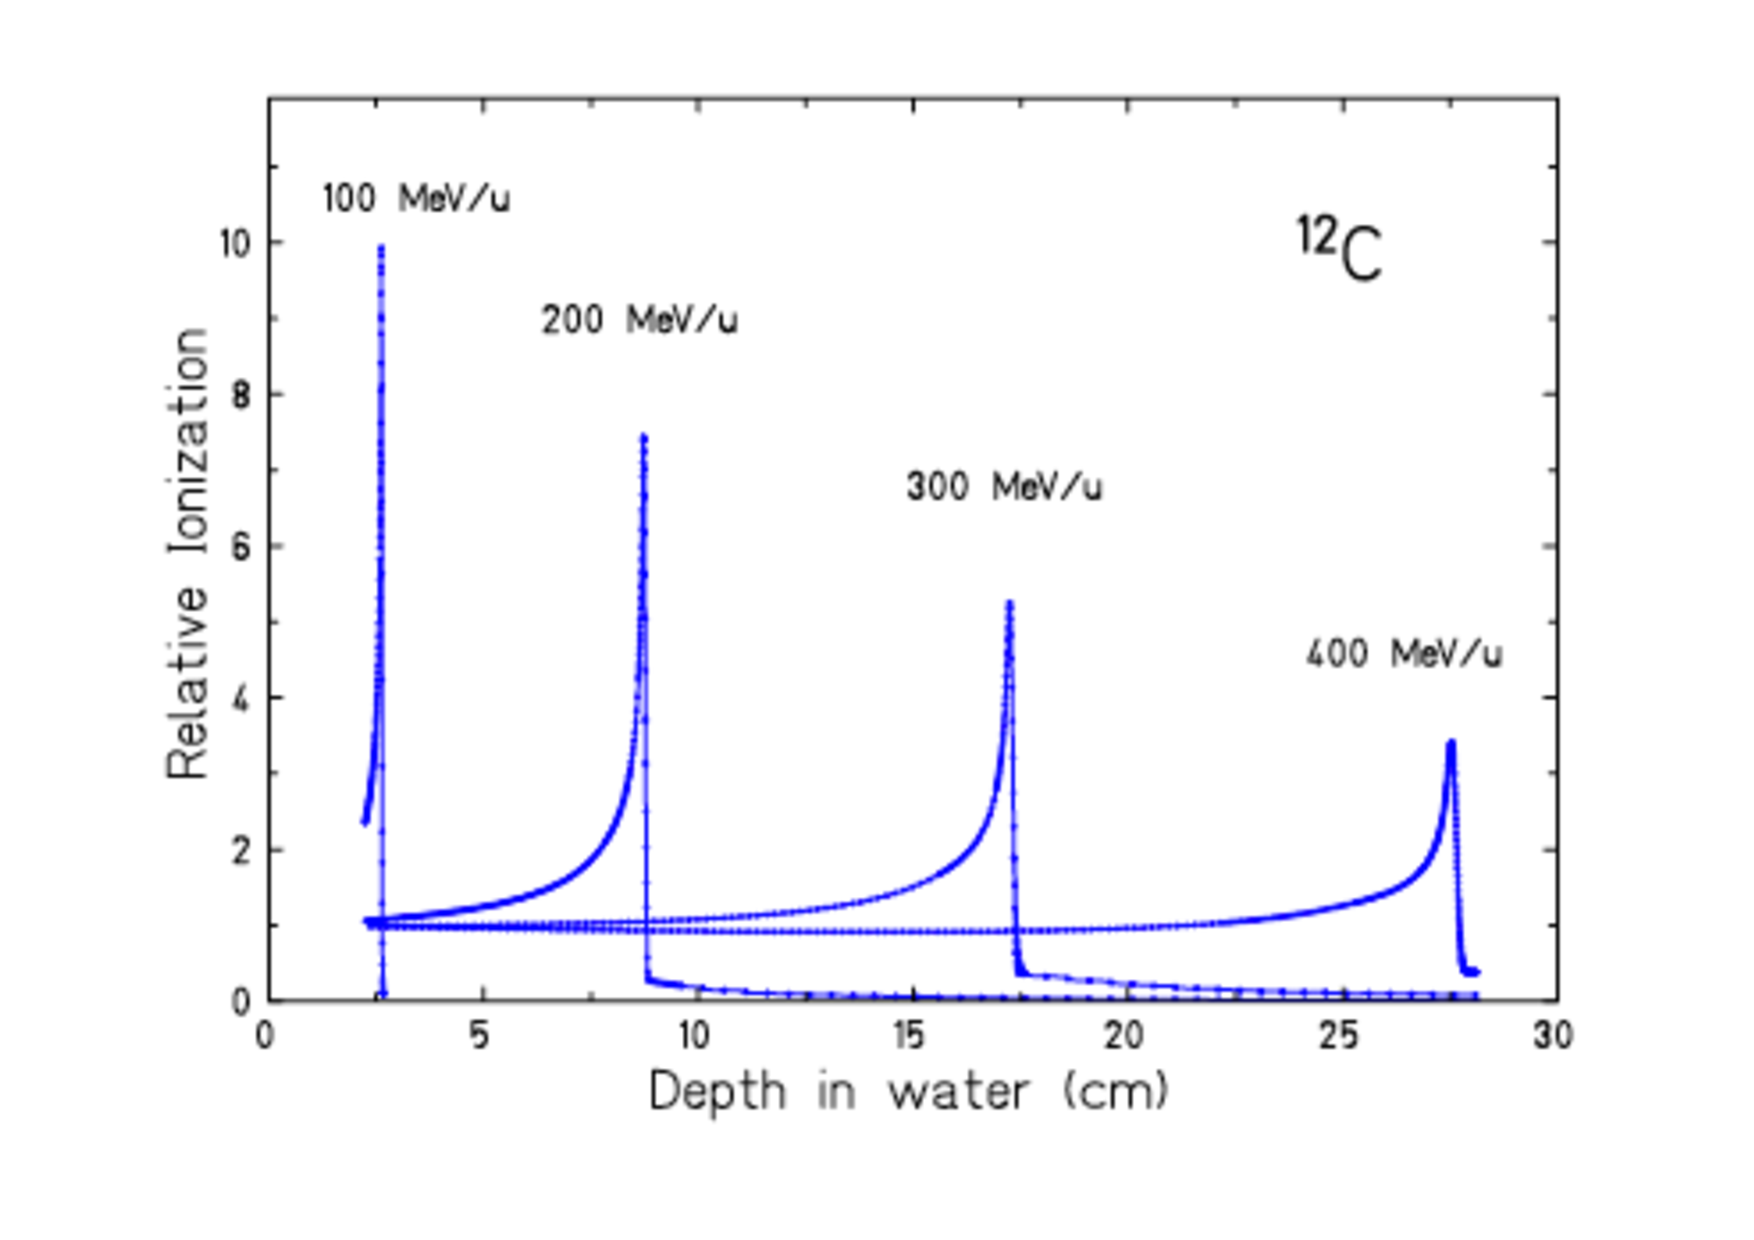
\includegraphics[width=1.2\linewidth, height = 6.05cm, trim = {1cm 0.4cm 0 0}, clip = true]{03_GraphicFiles/chapter1_Introduction/tailBragg_p.pdf}	
\caption{Measured relative ionizations for car\-bon ion beams stopping in water. In~\cite{Schardt2008}.}
\label{chap1::fig::TailBragg}
\end{subfigure}
\caption{Effects of nuclear interactions (first row) on proton (left column) and carbon ion (right column) beams and resulting dose distributions (bottom row).}
\label{chap1::fig::NuclearInt}
\end{figure}

Fragmentation processes have been deeply studied in nuclear physics and experimental data are available for many ion species at various energy~\parencite{Friedlander1982}. Dedicated studies for applications in radiotherapy started at Princeton~\parencite{MacCabee1974} with oxygen beams and were carried out for many years at the Bevalac in Berkeley~\parencite{Schimmerling1983, Schimmerling1989, Llacer1984, Llacer1990}, mainly with the neon beams used, at that time, for patient treatments. Analog studies were conducted later at the \gls{himac} facility~\parencite{Matsufuji2003, Matsufuji2005} and at \gls{gsi}~\parencite{Schall1996, Golovkov1997}: several ion species have been compared and carbon has been identified as the one offering the best fragmentation conditions. In addition, the positron-emitting fragments ($^{10}$C and $^{11}$C) can be used for online range monitoring with \gls{pet} techniques (see section~\ref{chap1::subsubsec::RangePET}). Results concerning the build-up characteristics of secondary fragments, also based on carbon ion irradiation of water targets, are published in~\cite{Haettner2006} and~\cite{Haettner2013}; in these works, 200 and 400~MeV/u ions have been used to investigate energy spectra and yields of the produced fragments at different angles and various depths along the beam path. A similar analysis has been carried out with 95~MeV/u carbon ion beam irradiation data collected at \gls{ganil}: in this case, \gls{pmma} thick targets (5, 10, 15, 20 and 25~mm) have been used~\parencite{Braunn2010, Braunn2011}. The obtained results have been compared to simulated data produced with fragmentation models implemented in Geant4 and mentioned in previous paragraphs, such as the \gls{bic} (based on the \gls{inc}) and the \gls{qmd} models, showing that model improvements were still needed to reproduce the experimental data.
Indeed, detailed information about fragmentation can be retrieved via Monte Carlo simulations and used to evaluate the impact on the delivered dose. As an example, in~\cite{Wroe2005} the authors studied in simulation the impact of nuclear reactions in the dose delivered with proton beams in different targets, like water, tissue equivalent plastic, and \gls{icrp} muscle, bone and adipose. Simulations published in~\parencite{Grassberger2011} of 160~MeV protons in water allowed to estimate the dose contributions given by primary particles (between 90\% and more than 99\% of the total depending on the range), with the remaining fraction of dose mainly connected to secondary protons and $\alpha$ particles: negligible dose is given by heavier fragments. A more intense dose contribution from heavier fragments is expected for carbon ion irradiation, but an accurate Monte Carlo simulation of these processes is still a challenge. The dose deposition in the distribution tail beyond the Bragg peak has been also studied in simulation: in~\cite{Francis2014}, for example, the dose connected to nuclear fragments has been estimated in 36\% of the total in the tail region. 

As mentioned, in addition to charged fragments, nuclear interactions also produce gammas, mainly originating from atomic de-excitation processes (prompt-gammas) or from the annihilation of positrons emitted by beta-emitter fragments ($^{10}$C, $^{11}$C, $^{13}$N, $^{14}$O, $^{15}$O), and neutrons, which can induce the emission of further gammas. All the secondary particles which can be absorbed by the target contribute to the total dispensed dose, while the others (with the exception of neutrons), escaping the target volume, can be exploited for non-invasive measurements of beam and target features. In particular, different techniques have been proposed and tested to measure secondary protons and gamma rays (both prompt-gammas and positron-annihilation gammas) with the aim of retrieving information about the ion range and obtain an online treatment verification. A detailed discussion about this topic will be given in section~\ref{chap1::subsec::uncertainty}.

Focusing on neutrons, which are produced in large quantities and over a wide energy range, they cannot be exploited for primary ion range monitoring since they are not correlated with the ion path in matter~\parencite{Testa2010}. The neutron signal can be used to retrieve dosimetric information in vivo, as reported in~\cite{Carnicer2014}: the research group at the \gls{cal} studied the secondary radiation in the proton ocular treatment room as a  function of the beam modulation, with a large volume ionization chamber. A strong correlation was found between the secondary ambient dose equivalent per proton dose and proton dose rate, which enables in vivo dosimetric verification independtly from the beam monitoring system. In any case, neutrons must be modeled with care in order to evaluate the safety measures to be implemented in treatment centers~\parencite{Newhauser2002}, as well as the implications in the delivered dose and secondary cancer probability~\parencite{Newhauser2011}. The dose contribution caused by secondary neutrons strongly depends on the beam delivery system (see section~\ref{chap1::subsec::beamDelivery} for the description of the beam delivery systems), as demonstrated in~\cite{Gottschalk2006}. In particular, passive elements used for beam shaping have been identified as one of the main sources of secondary neutrons contributing to the total delivered dose to the patient~\parencite{Yan2002}, so that in modern facilities deflecting elements are set after the passive modules in order to limit the neutron flux towards the target. It is interesting to notice that the amount of produced neutrons and resulting dose is comparable for protons and carbon ion irradiation, even if the neutron yield is higher for carbon ions: this is due to the different beam intensities used in clinics for the two species, with more than a factor 20 in favour of protons. Finally, if compared to photon standard radiotherapy at high acceleration voltage, the neutron dose associated to ion beam therapy treatments results to be smaller, as demonstrated in recent studies~\parencite{Schneider2015}. 

In the following section, the attention is focused on the biological aspects of this cancer treatment modality.


\subsection{Biological effects of ion beam therapy}\label{chap1::subsec::bioEffects} 
In addition to the already presented physical differences between photon radiation therapy and ion beam therapy treatments, a fundamental aspect to be addressed is the biological effect of such radiations. In the following, the main biological implications of radiation therapy are summarized with the aim of highlighting the favorable contribution given by charged particles with respect to photons and, at the same time, discuss some controversial points~\parencite{Paganetti2013}.

Any kind of radiation interacting and deposing energy in human tissues causes ionizations which lead to cellular and molecular effects. The effectiveness of ionizing radiation in curing cancer is based on the consequences produced by these ionizations, which can affect the double-helical DNA macro-molecules inducing various kinds of damages. In most of the cases, localized damages, also called strand breaks, can be repaired with cellular reparation processes. In case DNA breaks are in close proximity they can originate the so-called \glspl{dsb}, both with direct ionizations of indirect process (such as $\delta$-electron energy deposition). \figurename~\ref{chap1::fig::DNAdamages} shows a schematic view of the different kinds of DNA damages induced by radiations, together with their effects in case of  successful or unsuccessful reparation mechanisms. \glspl{dsb} are generally harder to be repaired and lead to cellular dysfunction and loss of genetic material, resulting in cell death or in the loss of reproductive capacity. It appears clear from this simplified presentation that not only the total absorbed dose, but also the ionization event distribution plays a major role in the determination of the radiation effectiveness~\parencite{Belli1992}.        
The absorbed dose is defined in ~\cite{ICRU1980, ICRU1998} as 

\begin{equation}
\mathrm{D} = \frac{\mathrm{d}\overline{\epsilon}}{\mathrm{d}m}
\label{chap1::eq::AbsDoseDef}
\end{equation}

where $\mathrm{d}\overline{\epsilon}$ is the mean energy imparted by ionizing radiation to matter of mass $\mathrm{d}m$. To be precise, the imparted energy must also be defined: in the same ICRU reports we find that 

\begin{equation}
\epsilon = R_{\mathrm{in}} - R_{\mathrm{out}} + \sum{Q}
\label{chap1::eq::impEnergyDef}
\end{equation}

with $R_{\mathrm{in}}$ and $R_{\mathrm{out}}$ the sum of the energies of all ionizing particles entering or leaving the volume, respectively, $ \sum{Q}$ the sum of all changes of the rest mass energy of nuclei and elementary particles in any nuclear transformations occurred in the volume due to the ionizing radiation.
As mentioned, for the same absorbed dose, the ability of killing tumor cells is linked to the nature of the delivered radiations via the ionization event distribution. It is useful here to introduce the concept of \gls{let} \myMarginnote{Linear \\ Energy \\ Transfer}, defined as the amount of energy deposited by a particle per track unit, directly related to the number of ionization per unit distance. In general, photons, x-rays and $\gamma$-rays are referred to as low-\gls{let} radiation, while the larger stopping power of protons and ions make them a high-\gls{let} kind of radiation. For low-\gls{let} radiation, the distribution of the caused lesions is approximately random, while it is more closely related to the particle track for high-\gls{let} primaries~\parencite{Lobrich1996} causing a clustering effect in radiation damage which has been verified to be effective for cell killing\parencite{Holley1996, Rydberg1996}. This is due to the nature of interactions of photons and ions in matter, already detailed in the previous section. 
Photons transfer energy to the cells by photo-electric of Compton interactions, with rather low cross-sections which determine a small number of ionization events per incident photon within the cell volume. Many photons are then required to depose the prescribed dose, and given the random spatial distribution of the photons in the irradiating beam, the resulting ionization distribution is almost homogeneous. The physical interactions of ions determine a completely different distribution of the deposited energy, localized along the ion path. The dose imparted in the radial direction is governed by freed electrons ($\delta$ or Auger electrons), emitted in ion-atom interactions, which are scattered by the medium atoms (electrons and nucleus) and cause secondary ionizations. The cross-section of these ionizations exhibits a maximum at about 100~eV, corresponding to a mean free path of a few nm. Given the DNA molecule size, this effect leads to a high probability of creating \glspl{dsb} or correlated single-strand breaks. %Thus, the lesion complexity increases with \gls{let}, and the strand breaks more concentrated in space are hardly repaired by the involved cells. 
Cell survival studies~\parencite{Tobias1982, Blakely1984} verified these theoretical considerations showing that heavy charged particles have an increased biological effectiveness compared to x-rays. These data are generally analyzed with a parameterization of the cell survival curve through a \gls{lq} model~\parencite{Hall2012}

\begin{equation}
S(D) = \mathrm{exp}(-\alpha D - \beta D^{2})
\label{chap1::eq::survivalPar}
\end{equation}
where S is the survival fraction, D is the absorbed dose and $\alpha$ and $\beta$ are parameters which are experimentally determined, or obtained via radio-biological models (see section~\ref{chap1::subsec::treatmentPlan}). The $\alpha/\beta$ ratio is linked to the radio-sensitivity of cells: the smaller it is, the larger the DNA repair capability will be. This is the rationale for fractionation in radiation therapy. Indeed, the total dose planned for the treatment of malignant cells is delivered in fractions along several days, because split doses have the advantage to spare normal tissues, with low $\alpha/\beta$ ratio, more than tumors, showing higher $\alpha/\beta$ ratio. 

\begin{figure}
\begin{subfigure}[t]{.4\textwidth}
\centering
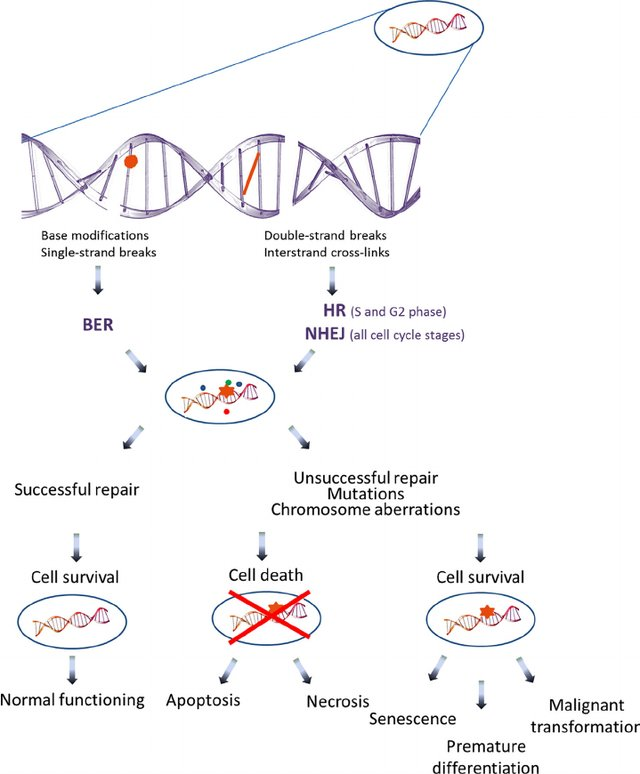
\includegraphics[width=0.99\linewidth]{03_GraphicFiles/chapter1_Introduction/DNAdamage.jpg}
\caption{Schematic representation of DNA damages caused by radiations. In~\cite{Arena2014}.}
\label{chap1::fig::DNAdamages}
\end{subfigure}
\begin{subfigure}[t]{.58\textwidth}
\centering
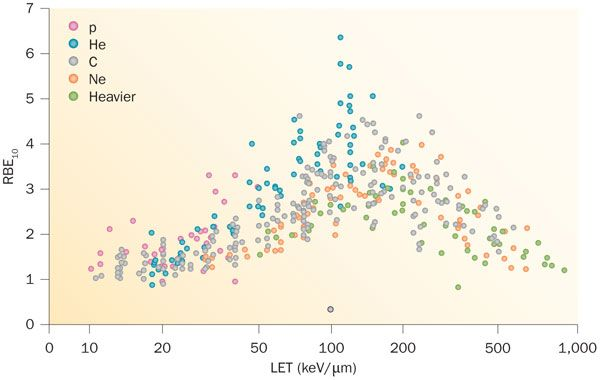
\includegraphics[width=0.99\linewidth]{03_GraphicFiles/chapter1_Introduction/rbeLET.jpg}	
\caption{\gls{rbe} dependence on \gls{let} for different particle species. \gls{rbe} is calculated at 10\% survival, \gls{let} values are given is keV/\charmum  ~in water. Different ions are represented in different colors. Data points are extracted from the \gls{pide} database. In~\cite{Durante2016}.}
\label{chap1::fig::rbelet}
\end{subfigure}
\caption{Ionizing radiations cause DNA damages in tissues, which are the basis for tumor radiation therapy. On the left side, the scheme presents the possible kind of damages induced by radiations on the cell DNA. The radiation effectiveness in killing cells is then related to the distribution of ionization events, which is all the more dense for high-\gls{let} primaries at low energies. The \gls{rbe} is then enhanced for this kind of radiation. On the right side, the \gls{rbe} is related to the \gls{let} for different ion species.}
\label{chap1::fig::NuclearInt}
\end{figure}
     
Given the complex scenario presented till here, it is clear that the physical absorbed dose is not sufficient to describe the effect of the delivered radiation treatment, and weighting factors based on radiation protection data have been introduced to account for both the biological properties of ions and the response of different tissues. However, \myMarginnote{Relative \\ Biological \\ Effectiveness} in order to transfer the experience from photon data to ion irradiation and to create a common evaluation parameter, the more powerful and versatile concept of \gls{rbe} has been introduced. The \gls{rbe} is defined as the ratio between the photon and ion doses necessary to produce the same biological effect (isoeffective dose):

\begin{equation}
\left. \mathrm{RBE} = \frac{D_{\mathrm{photon}}}{D_{\mathrm{ion}}}\right|_{iso}
\label{chap1::eq::rbeDef}
\end{equation}

where $D_{\mathrm{photon}}$ and $D_{\mathrm{ion}}$ are the absorbed dose for photon and ion irradiation. Notwithstanding the apparently simple definition, \gls{rbe} results to be a very complex quantity, but for the moment the only one really used in clinics. It depends on several physical and biological parameters, such as \gls{let}, dose, dose rate, fractionation scheme, particle type, target biological features (radiosensitivity, oxygen concentration, etc.)~\parencite{Durante2009}. As a result, the \gls{rbe} value changes along the primary ion path in matter, and is very difficult to be accurately predicted at the treatment planning stage. As an examples, the dependence on \gls{let} is shown in \figurename~\ref{chap1::fig::rbelet}.  Although an accurate prediction is difficult to be obtained, the overall evolution of the \gls{rbe} as a function of \gls{let} demonstrate a further advantageous feature of ions with respect to photons. From very low \gls{let} to approximately 100-200~keV/\charmum ~, the \gls{rbe} increases: an overkilling effect determines then a drop at very high \gls{let} values. Thus, \gls{rbe} is higher for low energetic high-\gls{let} particles, which cause larger ionization density as their velocity decrease. This effect means that in the Bragg peak region the biological effectiveness of such radiations is more pronounced with respect to the plateau entrance area, where healthy tissues are spared. The \gls{rbe} enhancement for increasing \gls{let} is at present neglected in proton therapy, and a constant value of 1.1 is implemented in the clinical routine. This point is deeply discussed in the last years, and many simulation results and models have been produced to verify or propose modification to this usage~\parencite{Giantsoudi2013, Sethi2014, Guan2015, Jones2015, McNamara2015, Giovannini2016}. Anyway,  it is verified that a significant increase in \gls{rbe} with respect to photons can only be achieved with heavier ions, as also shown by the experimental data reported in \figurename~\ref{chap1::fig::rbelet}. For this reason, clinical trials have been conducted at the Lawrence Berkeley Laboratory starting from 1975 on different ion species such as He, Ne, N, O, C, Si, Ar~\parencite{Castro1995}. Very heavy ions have the advantage of providing very-high \gls{let} (and so \gls{rbe}) in the Bragg peak region, useful to overcome cell killing capability limitation due, for example, to cell oxygenation effects (discussed in the following)~\parencite{Blakely1984}. On the other side, heavy ions also show very high \gls{let} in the entrance region, which is not desirable. These results led to the implementation of carbon ion therapy, together with proton therapy, as a good comprise between radio-biological enhanced effectiveness in the target region (carbon-ion \gls{rbe} ranges between 3 and 4 in the Bragg peak - see~\cite{Wilkens2008}) and limited \gls{let} in the entrance plateau. 
As outlined in previous lines, a further parameters to account for in the evaluation of the biological effects of radiations is the cell oxygen status \myMarginnote{Oxygen Enhancement Ratio}. If compared to healthy tissues, tumor masses can grow in size producing malignant cells, and tumor core generally show lower oxygen levels. Even if the reason is not completely explained, hypoxic conditions cause an increased cell radio-resistance, probably linked to the reduction of indirect DNA damages induced by radicals. This effect is quantified via the \gls{oer}, 

\begin{equation}
\mathrm{OER} = \frac{D_{\mathrm{hypoxic}}}{D_{\mathrm{aerobic}}}
\label{chap1::eq::oer}
\end{equation}

with $D_{\mathrm{hypoxic}}$ and $D_{\mathrm{aerobic}}$ the absorbed dose for normal and reduced oxygen level resulting in the same clinical effect. Its value is about 3 for conventional radiation~\parencite{Schardt2010}, while it is reduced for ion irradiation due to the increased \gls{rbe}, making them fundamental for curing tumors with hypoxic regions.

Only some of the biological aspects have been cited here, and all their clinical implications should be ideally taken into account for an accurate treatment planning. This is the reason why some of the points discussed here will be further addressed in section~\ref{chap1::subsec::treatmentPlan}. 

\subsection{Accelerators and beam delivery}\label{chap1::subsec::beamDelivery}

The goal of ion beam therapy is to treat deep-seated tumors with a conform dose distribution. Different ion species, hadrons and charged particles in general have been and are under study for the clinical application (neutrons, charged pions, antiprotons, helium ions - i.e. alpha particles -, heavier ions like lithium, oxygen, up to silicon ions), but only two are at present implemented for the patient treatments: protons and fully stripped carbon ions~\parencite{Degiovanni2015}. The ability of treating any kind of tumor at any depth in human body relies on the possibility of providing the employed particles enough energy to obtain a range of about 25~cm in soft tissues. The ions employed in treatment must be then accelerated to about 60-70\% of the speed of light ($\beta$ = 0.6-0.7, see~\cite{Durante2016}) via different acceleration techniques and machines. This translates into maximum energy values of the order of 200-250~MeV and 4500~MeV (i.e. 375~MeV/u) for protons and carbon ions, respectively~\parencite{Braccini2010}. In order to achieve the desired ion energy,  sizable accelerators are needed and different solutions have been explored; at present, cyclotrons and synchrotrons  are clinically implemented and available on the market. In the following, after a brief historical introduction, we sketch the main characteristics of the accelerators used in clinics, and we highlight the main features which are reflected in the treatment delivery. In addition to this, the beam delivery systems are described. Moreover, an overview of the main directions followed for the future acceleration and beam delivery techniques upgrade is provided. 

\subsubsection{Accelerators for ion beam therapy}\label{chap1::subsubsec::accelerators}
The way towards the possible application of ion beams in therapy \myMarginnote{Cyclotrons} (proposed only later by Wilson - see~\cite{Wilson1946}) was opened by the invention of the cyclotron by Ernest Orlando Lawrence in 1929~\parencite{Lawrence1932}, which added a magnetic field to the recently proposed linear accelerator~\parencite{Wideroe1928}. A cyclotron is composed of two hollow electrodes with a frequency-alternating voltage applied between them, which accelerates the charged particles at each revolution. The circular trajectory is obtained thanks to a fixed vertical magnetic field. A scheme of the main components of a cyclotron is sketched in \figurename~\ref{chap1::fig::cyclotron}.

\begin{figure}[!htbp]
\centering
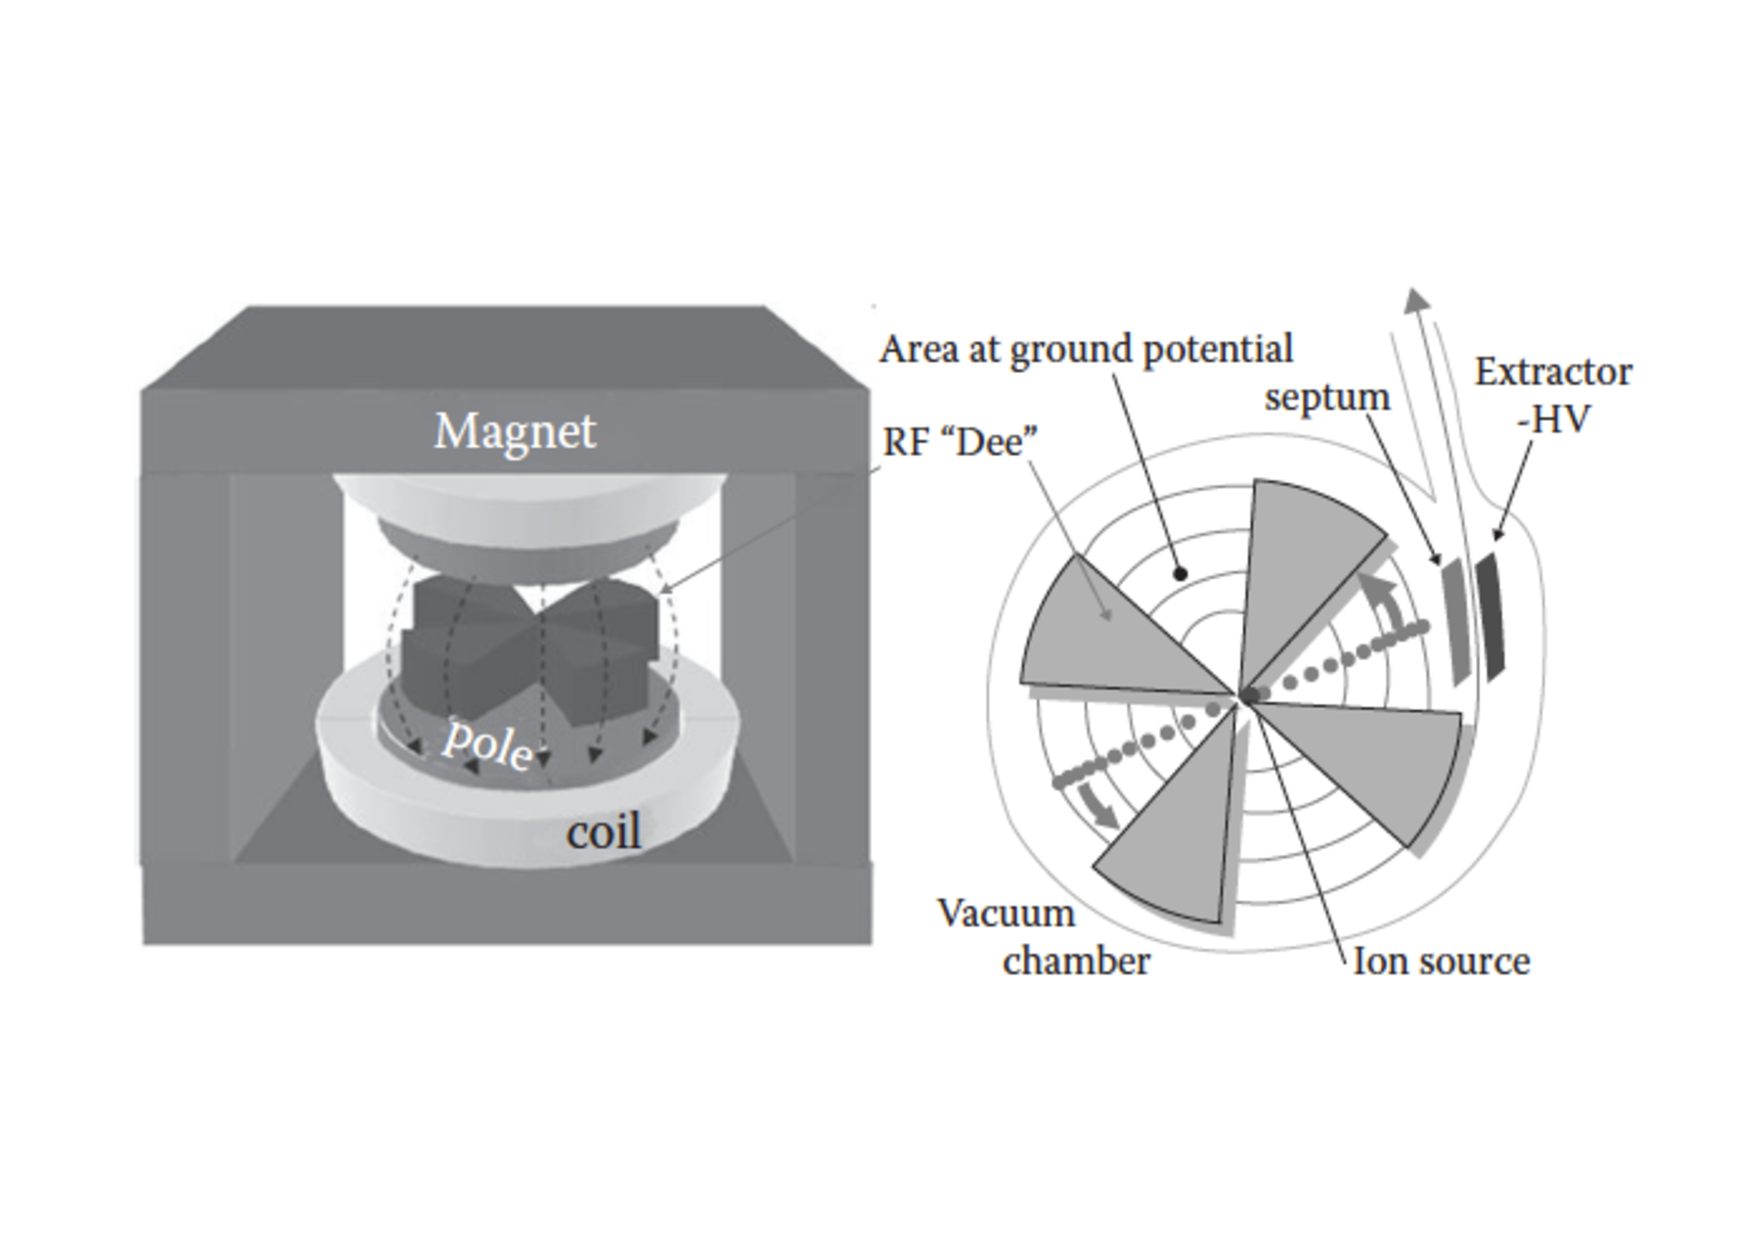
\includegraphics[width=0.7\textwidth]{03_GraphicFiles/chapter1_Introduction/cyclotron.pdf}
\caption{Schematic view of the main components of a cyclotron accelerator. On the left side the magnet is sketched together with the radio-frequency elements (\enquote{Dees}), which are also shown on the section depicted on the right side, with the ion source in the center. In~\cite{PaganettiBook2012}.}
\label{chap1::fig::cyclotron}
\end{figure} 

Nuclear physics saw a paramount development thanks to this invention, but also in the medical field the impact was remarkable. Already in 1935, Lawrence produced the first cyclotron-originated radionuclides, then used for radiotracing, diagnosis and treatment. The first cyclotron-based treatment was performed with fast neutrons (i.e. with kinetic energies between a few MeV and a few tens of MeV) in 1938, following a paper by Gordon Locher who underlined the therapeutic potentialities of neutrons~\parencite{Locher1936}; the neutrons were produced by bombarding a beryllium target with cyclotron-accelerated deuterons~\parencite{Stone1940}. The unfavorable depth-dose distribution of neutrons and the difficulties linked to their collimation finally led to abandon the neutron treatments in 1948~\parencite{Stone1948} and move towards proton-beam treatments in the 50's: neutrons were revised in 1965 by Catterall in London~\parencite{Catterall1971} and are still used today in \gls{bnct} techniques~\parencite{Barth2005, Nedunchezhian2016}. As already mentioned in section~\ref{chap1::sec::ionBeamTher}, the first proton therapy treatment was conducted by Cornelius Tobias,  and John Lawrence with the Lawrence cyclotron in 1954~\parencite{Tobias1955, Tobias1958}. Between 1954 and 1974, more than 100 patients were treated in Berkeley with cyclotron-accelerated protons. In parallel, in 1957 the first tumor was irradiated with protons at the Uppsala cyclotron in Sweden~\parencite{Larsson1962}, and an intensive proton therapy program, leaded by Robert Wilson, was started in Harvard with a new-built cyclotron~\parencite{Wilson2004}. Following these first experiences, new physics laboratories decided to set up proton beams for therapy (USSR, Japan, Switzerland), until the creation of the first hospital-based center, built at the Clatterbridge Oncology Center in the United Kingdom, which started operating in 1989 with a 62.5~MeV cyclotron. This historical overview shows how the cyclotron technology has soon spread all over the world, not only in research centers, but also for therapy purpose. The present cyclotron machines, which are now commercially available by different providers,  still rely on the same accelerating principle as the first Lawrence system, but the technology has greatly advanced.  In particular, the vertical magnetic fields in charge of bending the particles on a spiral trajectory has been improved, giving the beam the desired transverse compactness. Moreover, the beam extraction efficiency has been improved, and multiple extractions are now possible to supply different transport lines.
Moreover, synchrocyclotrons are a solution compatible with hadrontherapy applications. Based on the cyclotron accelerating principle, a synchrocyclotron presents a variable frequency for the alternating voltage which is used to compensate for relativistic effects when the accelerated ions approach the speed of light. Such a solution has the advantage of allowing for the creation of more compact systems with high magnetic fields, and is at present exploited for commercial accelerators by the main providers.  
In addition to cyclotrons and synchrocyclotrons, other accelerating machines \myMarginnote{Synchrotrons} initially developed for fundamental research have been translated to medical applications and are nowadays knowing a large diffusion: the synchrotrons. While the cyclotron present a fixed-value magnetic field, so that the radius of the beam trajectory increases during the acceleration process, in the synchrotron the trajectory radius is kept constant thanks to the variation of the bending magnetic field. The boost is provided by radio-frequency cavities, based on the same principle as the one composing linear accelerators: the radio-frequency increases to follow the particle revolution speed, and this acceleration principle allows to overcome the cyclotron energy limitation, as well as to obtain beam at different energies by tuning the extraction process. The invention is based on the independent ideas of Vladimir Veksler~\parencite{Veksler1944} and Edwin McMillan~\parencite{McMillan1945}: the latter both coined the name of the machine in its letter, and constructed the first electron synchrotron in 1945 in Berkeley. Some years later, the first proton synchrotron was designed in 1952 by Sir Marcus Oliphant, who already published a preliminary sketch of the machine in 1943~\parencite{Oliphant1943}. As for the cyclotron case, several years have been required to see the construction of the first hospital-based hadrontherapy facility using a synchrotron. The first center was built at Loma Linda University in California, were a 7-m-diameter synchrotron constructed by Fermilab was installed and started treating patients in 1990. The center has been a pioneer in the field also for the presence of three 10-m-diameter rotating gantries.  
After the clinical studies performed at the University of Tsukuba, in Japan, between 1983 and 2000, with the treatment of about 700 patients with synchrotron proton beams, a second hospital-based center was built and equipped with an Hitachi synchrotron and two rotating gantries. 
Since the first use of synchrotrons for treatment purpose, several improvements have been achieved in the accelerator technology to better adapt its features to the hadrontherapy needs. In particular, the beam size can be now reduced with strong focusing optics, and the beam energy can be varied on a single spill basis (1-2~s).%, in contrast to the first machines for which 1-2~s were needed to modify the spill energy.   
At present, all the hadrontherapy facilities in operation are based on circular accelerators (cyclotrons and synchrotrons): proton beams are produced with both the solutions, while only synchrotron-produced carbon-ion beams are used. In \figurename~\ref{chap1::fig::acceleratorSize} the size of different accelerators design is compared (CABOTO is still at the design stage, the \gls{iba} superconducting carbon cyclotron is under design in France, while \gls{hit}, \gls{cnao} and the SIEMENS accelerator are at present in operation).

\begin{figure}[!htbp]
\centering
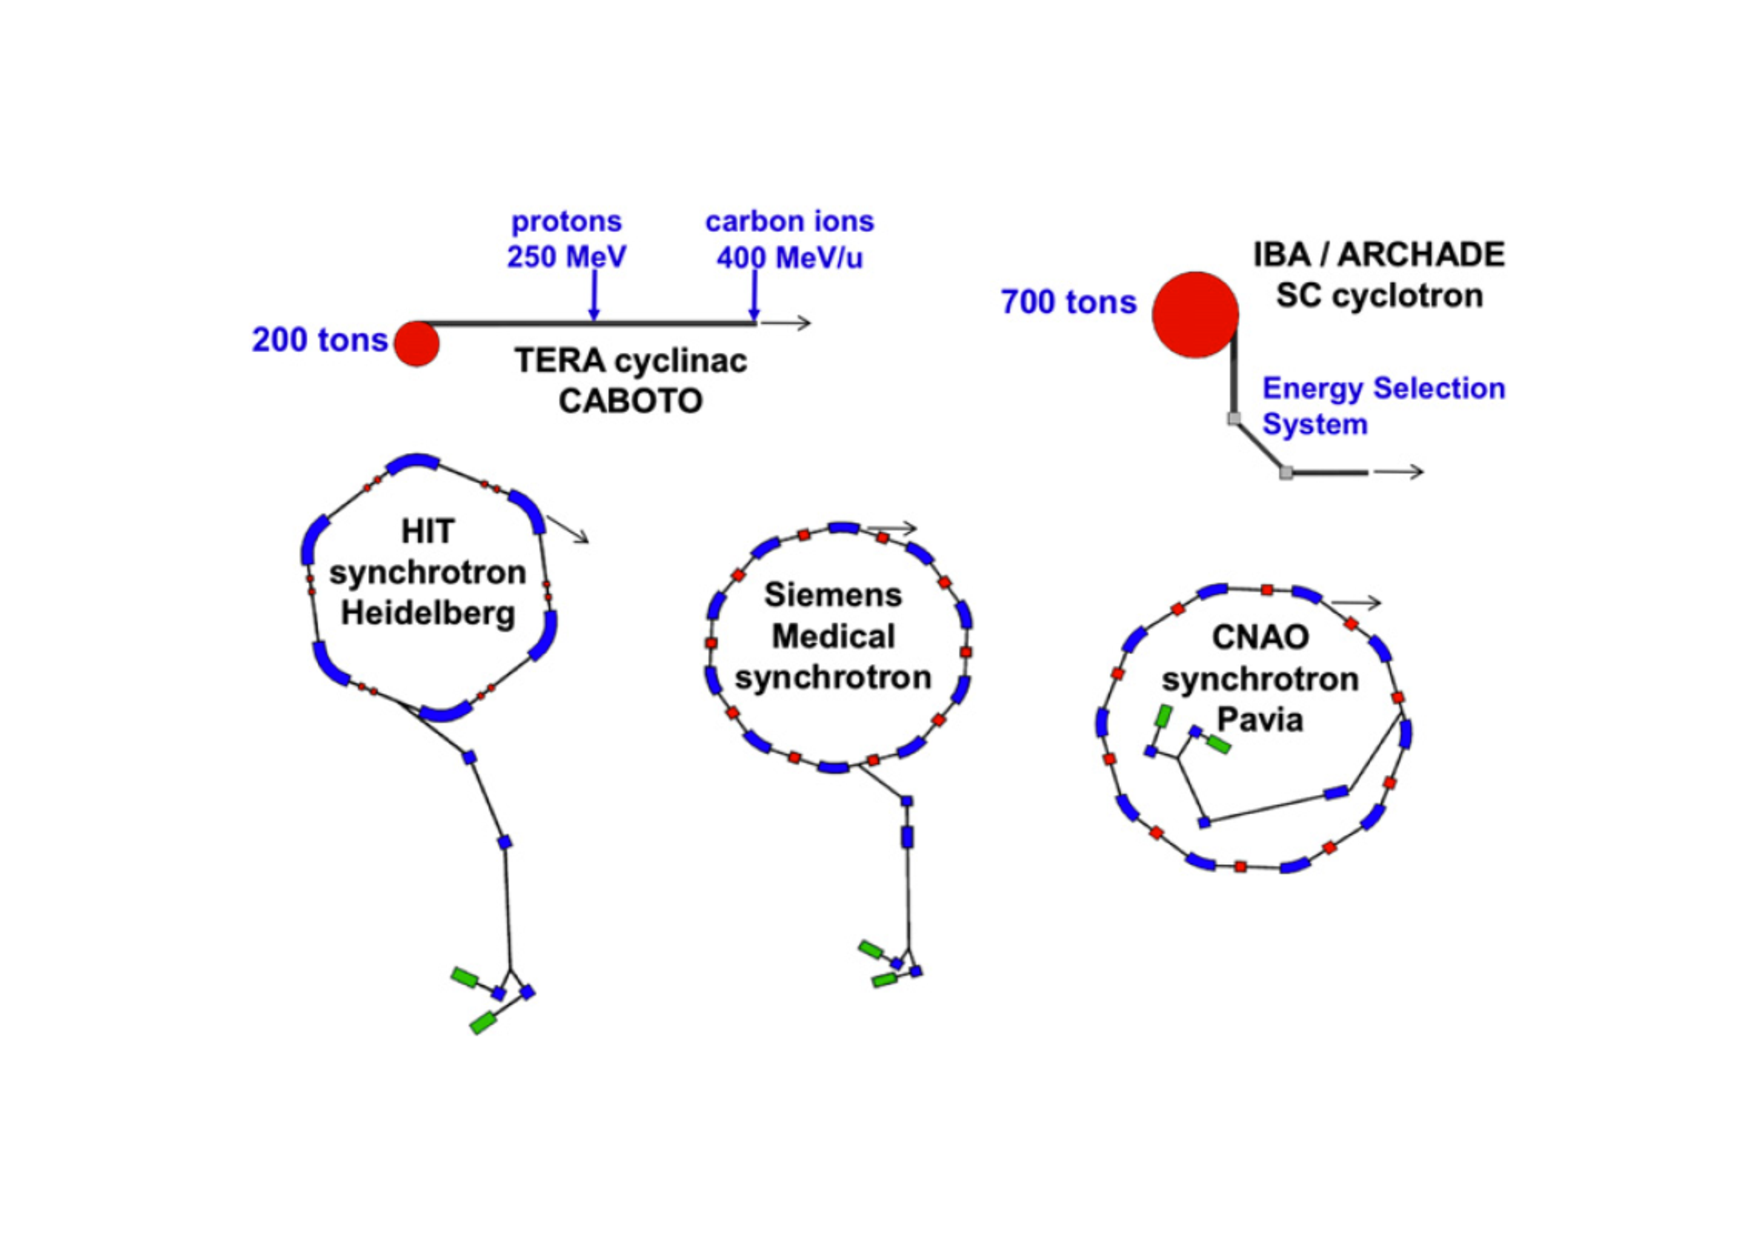
\includegraphics[width=0.7\textwidth]{03_GraphicFiles/chapter1_Introduction/acceleratorSize.pdf}
\caption{Comparison of the size of various ion accelerators for hadrontherapy. CABOTO is a cyclinac studied by the TERA Foundation; the superconducting cyclotron, designed by \gls{iba}, is under installation in Caen, France, within the ARCHADE project; \gls{hit} and \gls{cnao} are in operation in Heidelberg, Germany and Pavia, Italy, respectively; the SIEMENS synchrotron is installed in Marburg and Shangai. In~\cite{Amaldi2010}.}
\label{chap1::fig::acceleratorSize}
\end{figure} 

In the last years, novel approaches have been proposed \myMarginnote{Novel acceleration approaches} to improve the present accelerators and beam features, mainly for what concerns the beam quality and the machine size and cost. It is worth to mention the \gls{ffag} accelerator, which combines the fixed magnetic field and variable radio-frequency with separated sector magnets~\parencite{Sheehy2016}. This approach allows for the production of higher intensity beams with respect to synchrocyclotrons, and for the variation of the extracted beam energy at high repetition rate. Some designs have been proposed for hadrontherapy applications in the last decade~\parencite{Antoine2009, Peach2010}, but the present machine size still limits its spread in treatment centers. 
Furthermore, linear acceleration approach has been proposed since 1991 in both \enquote{all-linac}~\parencite{Lennox1991, Hamm1991} and \enquote{cyclinac}~\parencite{Amaldi2009b} solutions. In addition to the compactness, the main advantage of linacs is the possibility to continuously vary the output beam energy on a pulse to pulse basis; in addition to this, there is neither the need for complex injection or extraction systems, such the ones used in synchrotrons, nor the need of an energy passive modulation technique as the one used in cyclotrons (see section~\ref{chap1::subsubsec::BeamDel}). An extended description of linear accelerators for hadrontherapy is given in~\cite{Amaldi2009a}. Following the first successful prototypes tested by the TERA Foundation and the Italian \gls{infn} in the last twenty years~\parencite{Amaldi2004, Ronsivalle2011}, the \gls{cern} spin-off company \gls{adam} is proposing a commercial solution called \gls{light}. A further solution can be given by the \gls{dwa}~\parencite{Caporaso2009}, where the acceleration tube is made of High Gradient Insulator disks alternated with conducting elements. A laser pulse is used to activate the switching units connected to these conducting modules. Very interesting thanks to a reduced size, this acceleration scheme still suffers beam focusing issues; moreover, it presents very short pulses which force a very precise selection of the number of ion per pulses at the source level. Finally, the electric field needed for reducing the machine size till 2-2.5~m is of the order of 100~MV/m; this challenging value has not been achieved yet, even if a prototype is under study at the \gls{llnl}, with promising results~\parencite{Hettler2013, Zografos2013}. Another attractive technique is the so-called \enquote{laser driven} acceleration, based on the use of short and powerful laser pulses irradiating a thin target, with the generation of a plasma field~\parencite{Tajima2009}. The electrons emerging form this plasma are able to induce a strong electric field which accelerates the protons (or ions). Again, this solution would allow for the creation of very compact systems, with relatively simple and light beam optics, but some issues are still under study to be solved; in particular, the accelerated beam has an almost continuous energy spectrum which forces to implement energy modulation solutions to be adapted to treatment purposes. 

\subsubsection{Beam time structure}\label{chap1::subsubsection::beamTimeStruct}

A particle beam can be described by a set of quantifying parameters which relates to single particle properties or to a collection of particles. In addition to the beam energy (which should be defined as an energy spectrum), beam current (which describes the beam intensity as the flux of particles per time unit) and emittance (transverse size and momentum), it is worth to describe in details what is defined as time structure. A basic distinction is made between continuous beams and bunched beams. Whenever particles are accelerated by means of radio-frequency varying fields, the accelerating machine output is a bunched beam, composed of bunches with fixed time length. Concerning the acceleration systems employed to produce clinical beams, synchrotron and cyclotrons (or synchro-cyclotrons) present strongly different time structures. In order to give an overall description of the typical time features of synchrotron- and cyclotron-produced beams, it is possible to distinguish between micro- and macro-structure. The macro-structure describes cycles of several radio-frequency periods, while the micro-structure gives the details of the particle time distribution within the same radio-frequency period. By comparing the two cited kinds of accelerators, it is possible to approximate the cyclotron-produced beams as continuous, with a macro-structure characterized by sub-millisecond periods (depending on the specific machine). In contrast, synchrotrons produce pulses which are separated in periods of several seconds, so that during the irradiation the active beam time is limited. Each accelerator pulse (for both cyclotrons and synchrotrons), corresponding to one \gls{rf} period, contains several micro-bunches, creating the micro-structure. For cyclotrons, micro-bunches duration is in the ns scale, while a synchrotron micro-bunch can last several tens of ns. The period separating micro-bunches varies in the range of tenths of ns for cyclotrons till hundreds of ns for synchrotron beams. 

Table~\ref{chap1::tab::beamTime} shows the orders of magnitude for the beam time structure for some particle accelerators used in the clinical routine. The differences between synchrotrons, cyclotrons and synchro-cyclotrons are evident. In addition, the beam typical intensity is reported.

\begin{table}[!htbp]
\centering
\caption{Orders of magnitude of main time structure parameters for some accelerators used in clinics. Reproduce from~\cite{Krimmer2017}.}
\label{chap1::tab::beamTime}
\begin{tabular}{P{2cm} P{2cm}  P{1cm} | P{1cm} P{2cm} P{2cm} P{2cm}}
\toprule
\rowcolor{myColorMainA!20} 
 	& &  \multicolumn{2}{c}{\textbf{Synchrotron} }& \textbf{Cyclotron C230 \gls{iba}} & \textbf{Cyclotron Varian} & \textbf{Synchro-cyclotron S2C2 \gls{iba}}\\
& & \underline{$^{12}$C} & \multicolumn{4}{c}{\underline{Protons}} \\
\midrule
\multicolumn{2}{l}{\textbf{Typical intensity (ions/s)}} & 10$^7$ & 10$^9$ & 10$^{10}$ & 10$^8$ - 10$^{10}$& $\sim$10$^{10}$ \\
\midrule
\textbf{Macrostruct.} & Period (s) & \multicolumn{2}{c}{1-10} & \multicolumn{2}{c}{/} & 10$^{-3}$ \\
\midrule
 & Bunch width & \multicolumn{2}{c}{20-50} & 1-2 & 0.5 & 8 \\
\textbf{Microstruct.}  &  Period (ns) & \multicolumn{2}{c}{100-200} & 10 & 14 & 16\\
 & Ions/bunch & 2-5 & 200-500 & 200 & 2-200 & 4000 \\
\bottomrule
\end{tabular}
\end{table}      

An accurate knowledge of the beam time structure is of utmost importance for the optimization of the interface to the beam delivery systems (see section~\ref{chap1::subsubsec::BeamDel}), for the treatment planning, as well as for treatment monitoring purpose. The design of detectors able to exploit the emission of secondary particles to retrieve beam range and dose information must account for the beam time structure in order to evaluate the best solution to deal with signal background, counting rate and read-out channel occupancy. This topic will be further discussed in section~\ref{chap1::subsec::uncertainty} where the sources of uncertainties affecting ion beam therapy treatment are described and the detection monitoring solutions are presented. In particular, for the specific case of \gls{pg} detection (one of the main topic of this thesis work), a complete overview is given in chapter~\ref{chap::2}. 

\subsubsection{Beam delivery systems}\label{chap1::subsubsec::BeamDel}

Once accelerated, the high-energetic ions must be delivered to the patient in order to be conform to the treatment specification, focusing the provided dose on the \gls{ptv}. As described and detailed in section~\ref{chap1::subsec::Physics}, the beam range can be varied by modulating the primary particle energy with the aim of covering the whole tumor volume. The Bragg curve obtained with a monoenergetic beam is called \enquote{pristine Bragg curve}, and can be used to irradiate a section of the target volume at a given depth. The superposition of several pristine Bragg curve is necessary to deliver the prescribed dose to the tumor, which has been previously modeled in three dimensions. In particular, the beam energy spectrum has to be spread in order to increase the axial dimension of the peak region, in the so-called \gls{sobp}. At the same time, the beam fluence must be adapted to avoid over-irradiation of the entrance region. An example of \gls{sobp} is given in \figurename~\ref{chap1::fig::pristine_sobp}. Note that the distal spot has a significantly higher fluence than proximal ones, since there is no contribution of higher energy particles. This will have an influence on the sensitivity of the method used to control the position of the distal part of the \gls{sobp}, as discussed in section~\ref{chap1::subsec::uncertainty}. 

\begin{figure}[!htbp]
\centering
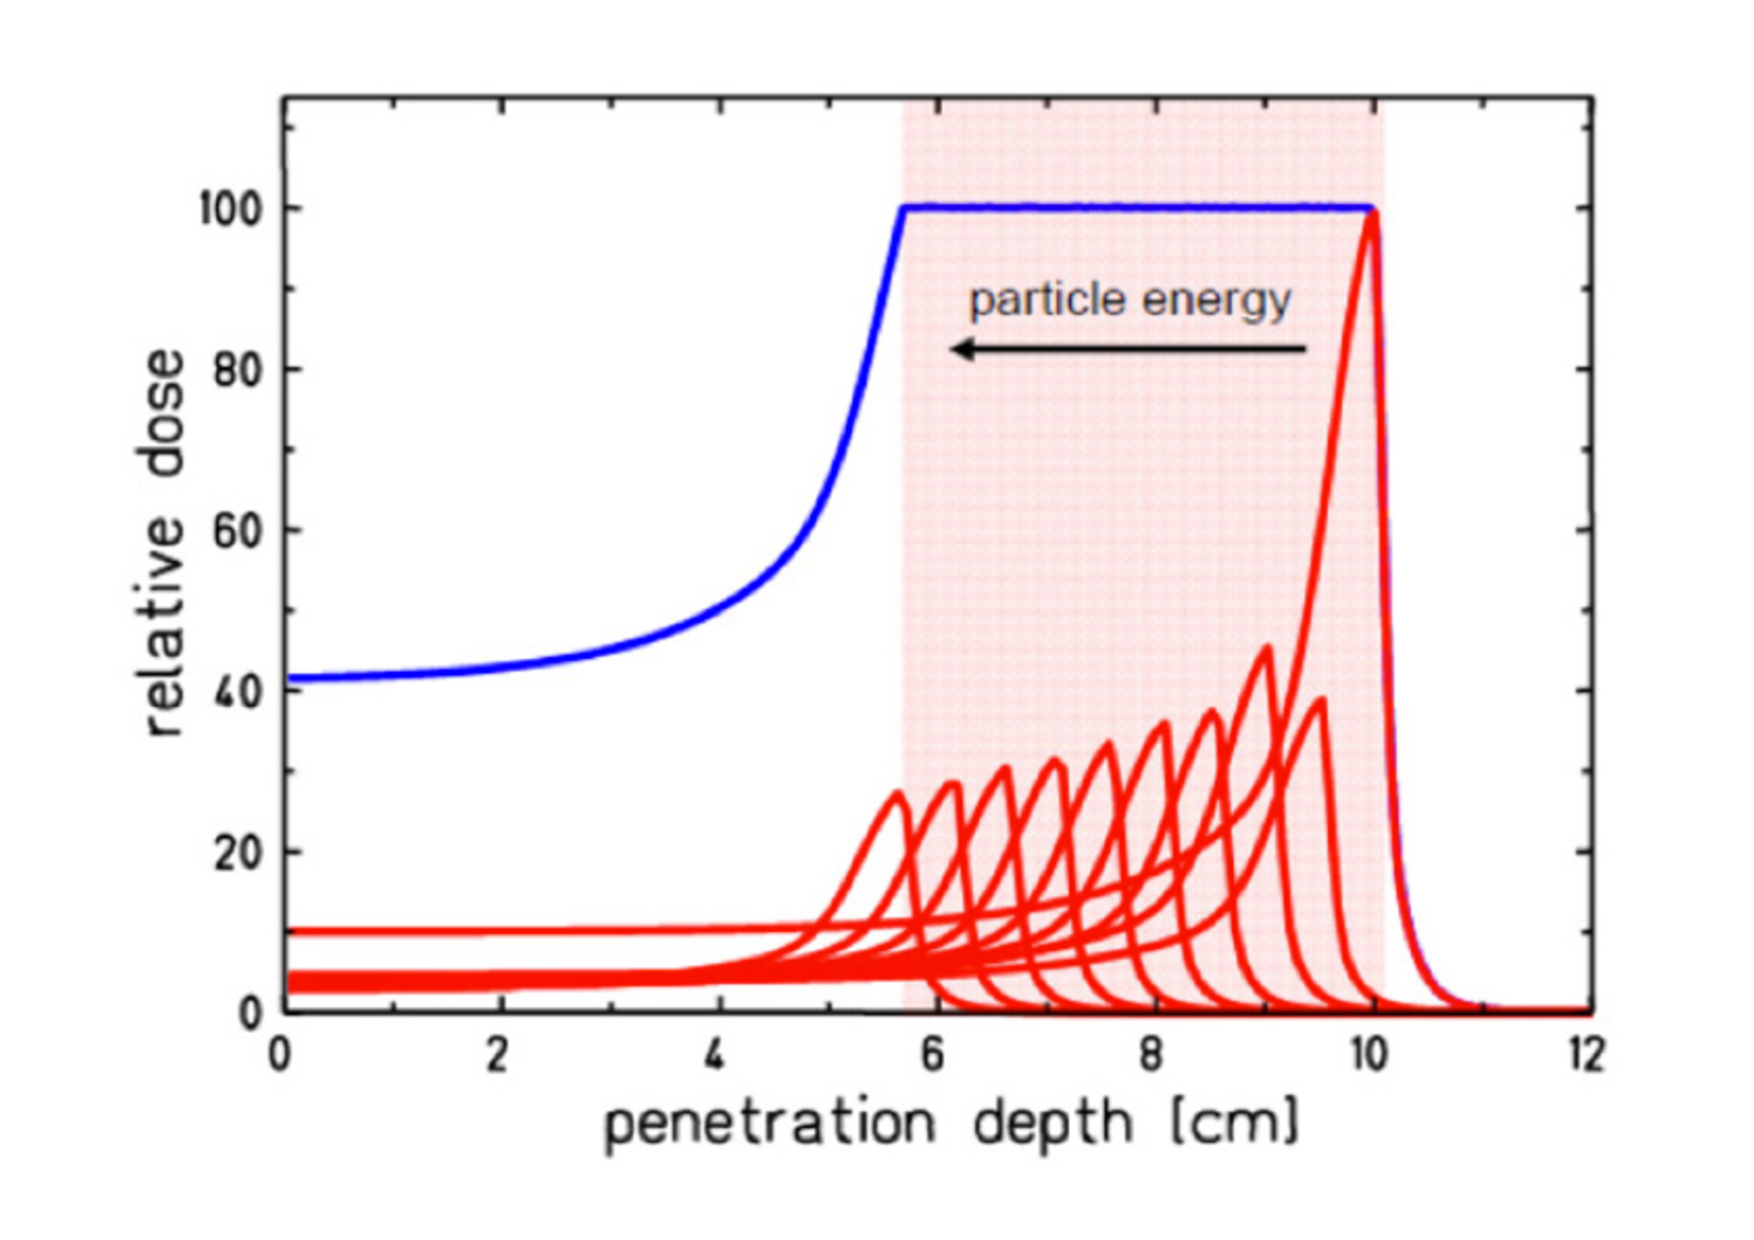
\includegraphics[width=0.7\textwidth]{03_GraphicFiles/chapter1_Introduction/pristine_sobp.pdf}
\caption{Example of \gls{sobp}. The target region is highlighted and the discrete pristine peaks composing the \gls{sobp} are sketched in red. In~\cite{Durante2016}.}
\label{chap1::fig::pristine_sobp}
\end{figure} 

All the described tasks are in charge of the beam delivery system, which must be optimized to interface with the accelerator and to the patient by transporting the beam to the treatment area and adjusting its features to obtain the desired dose distribution. 
The delivery systems implemented in clinics are based on two main strategies: passive beam modulation and active scanning. For an extensive presentation of this topic, refer to~\cite{Gottschalk2008}. The technique must be chosen according to the accelerator machine: it is important to remind that cyclotrons provide fixed energy beams with pulses separated by tens of nanoseconds, while in a conventional synchrotron the energy can be varied cycle by cycle, with short pulses generally separated by 1-2~s dead-time (see section~\ref{chap1::subsubsection::beamTimeStruct}). 

The passive beam delivery approach \myMarginnote{Passive beam shaping} generally applies to cyclotron-produced beams, and its principle is sketched in \figurename\ref{chap1::fig::passiveDelivery}. The beam extracted from the accelerator is fixed in size and energy, and is first broadened by scattering devices. Afterwards, a range modulator (generally a rotating wheel) is used to spread out the mono-energetic Bragg peak with the aim of covering the whole target thickness. The wheel periodically inserts material of varying thickness into the beam line, resulting in a range modulation with the desired features. The obtained \gls{sobp} can be shifted as a whole thanks to the addition of range shifters of fixed thickness. After the energy (range) adaptation, the beam is shaped according to the \gls{ptv} definition with collimators (often multi-leaf) and compensators, which are specific to each patient and irradiation port.  

\begin{figure}[!htbp]
\centering
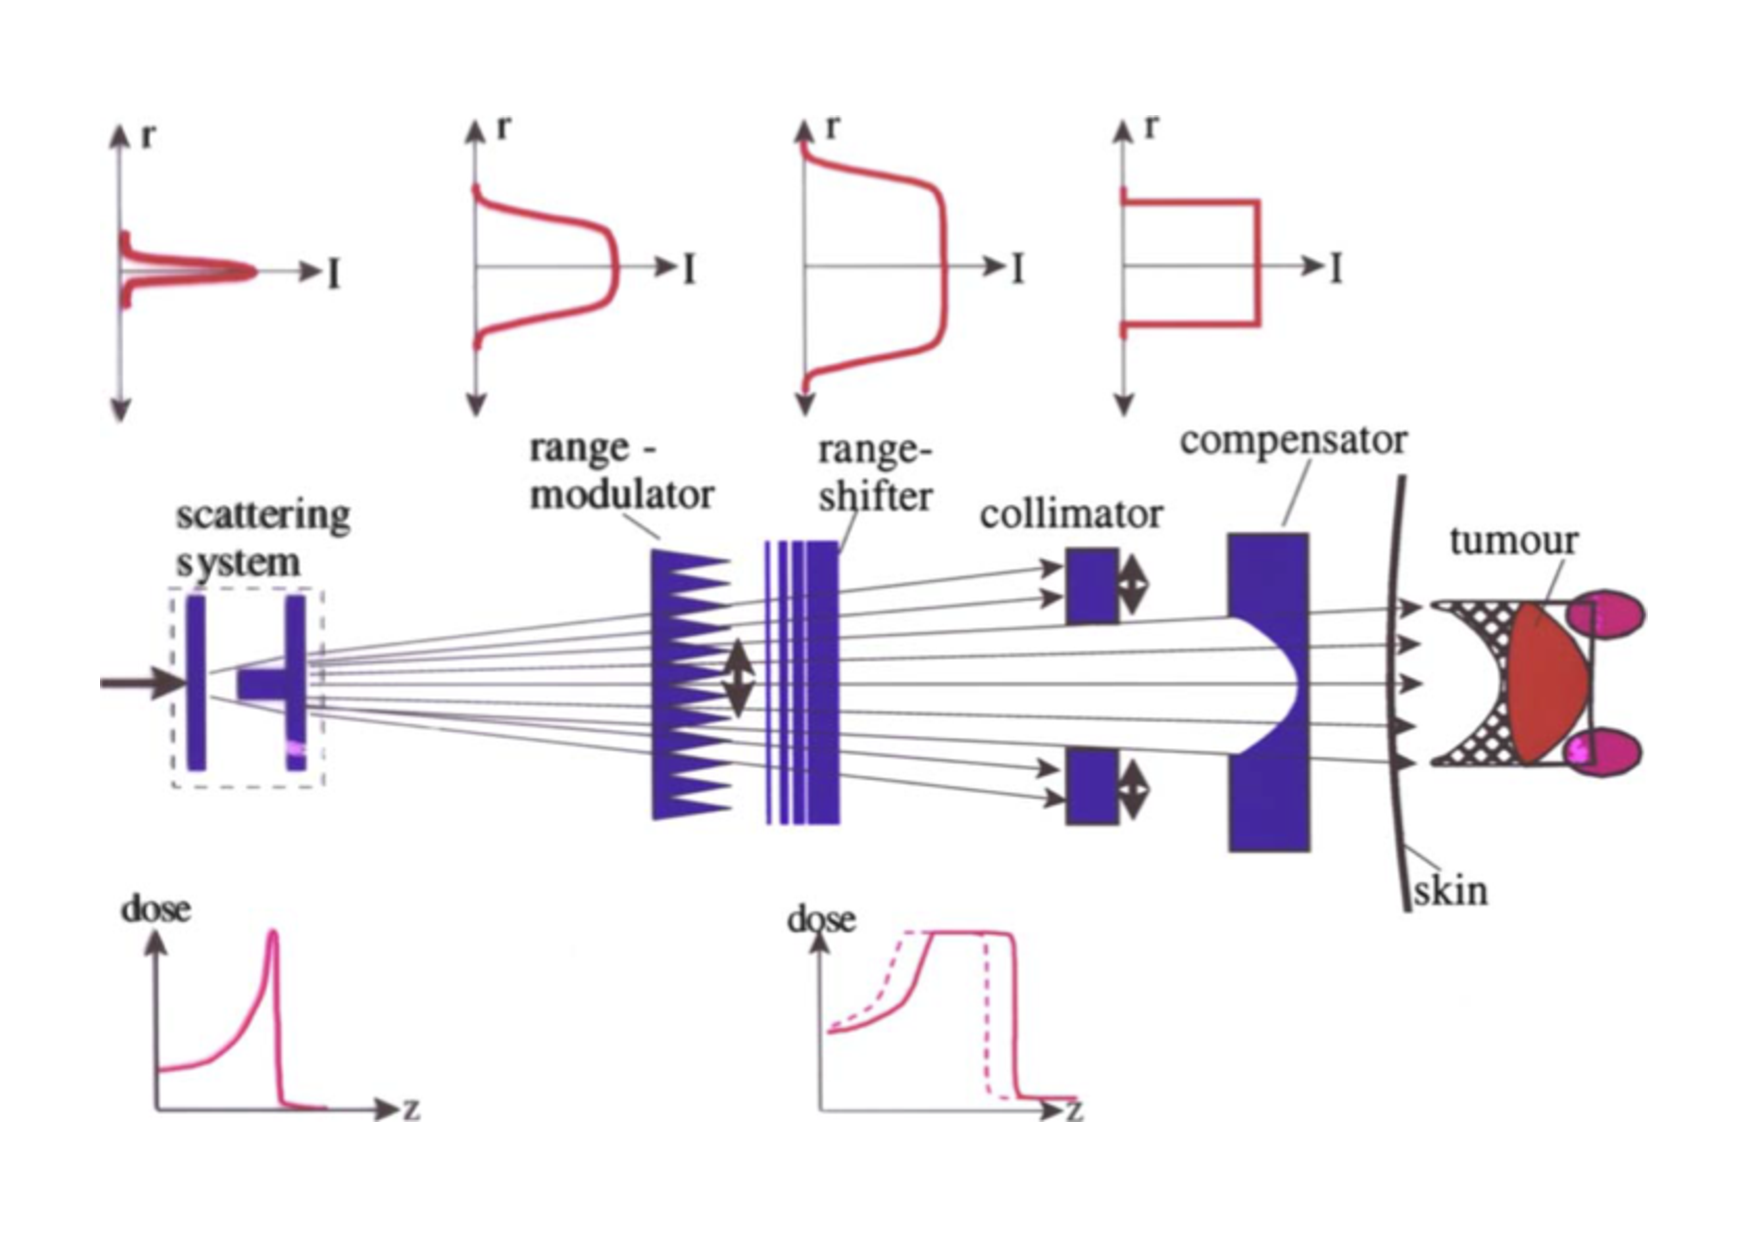
\includegraphics[width=0.7\textwidth]{03_GraphicFiles/chapter1_Introduction/passiveDelivery.pdf}
\caption{Schematic view of a fully passive beam delivery system. In~\cite{Schardt2010}.}
\label{chap1::fig::passiveDelivery}
\end{figure} 

The passive beam delivery technique presents two main disadvantages with respect to the active delivery described in the following. First, the structure of the created \gls{sobp} is fixed and the depth-dose can only be tailored to the distal end of the target volume and not to the proximal end, given the fact that the \gls{sobp} can only be shifted towards the entrance region. This feature automatically leads to a considerable dose given to normal tissues outside the target volume, in particular in the proximal part, as illustrated by the hatched region in \figurename~\ref{chap1::fig::passiveDelivery}. Second, the amount of material inserted in the beam line causes nuclear interactions which lead to the creation of secondary high-\gls{let} fragments (mainly neutrons), affecting the dose delivered to the entrance region. Third, each collimator/compensator are specifically designed for each patient irradiation port, which leads to complex and costly manufacturing for such devices.
The main asset of passive beam delivery is that the whole target volume is irradiated at once, which leads to shorter irradiation times. This last point is quite important for the irradiation of large \glspl{ptv}.

When the beam is produced with a synchrotron, \myMarginnote{Active beam scanning} the possibility to switch the energy from pulse to pulse makes feasible an active target scanning and beam range adaptation. Active beam delivery is also possible with cyclotron-accelerated beams, but the beam energy is modulated with degrading passive elements, and a spectrometer is needed for energy selection, at the cost of an important intensity reduction. The active beam delivery systems exploit the electrical charge of the accelerated particles to deflect the beam laterally through magnets and perform a scan of the defined treatment field. A schematic view of an example of active delivery system is provided in \figurename~\ref{chap1::fig::activeDelivery}. The target volume is divided into iso-energetic layers which are irradiated sequentially by deflecting the beam with dipoles in order to fully cover a grid of pre-defined voxels.              

\begin{figure}[!htbp]
\centering
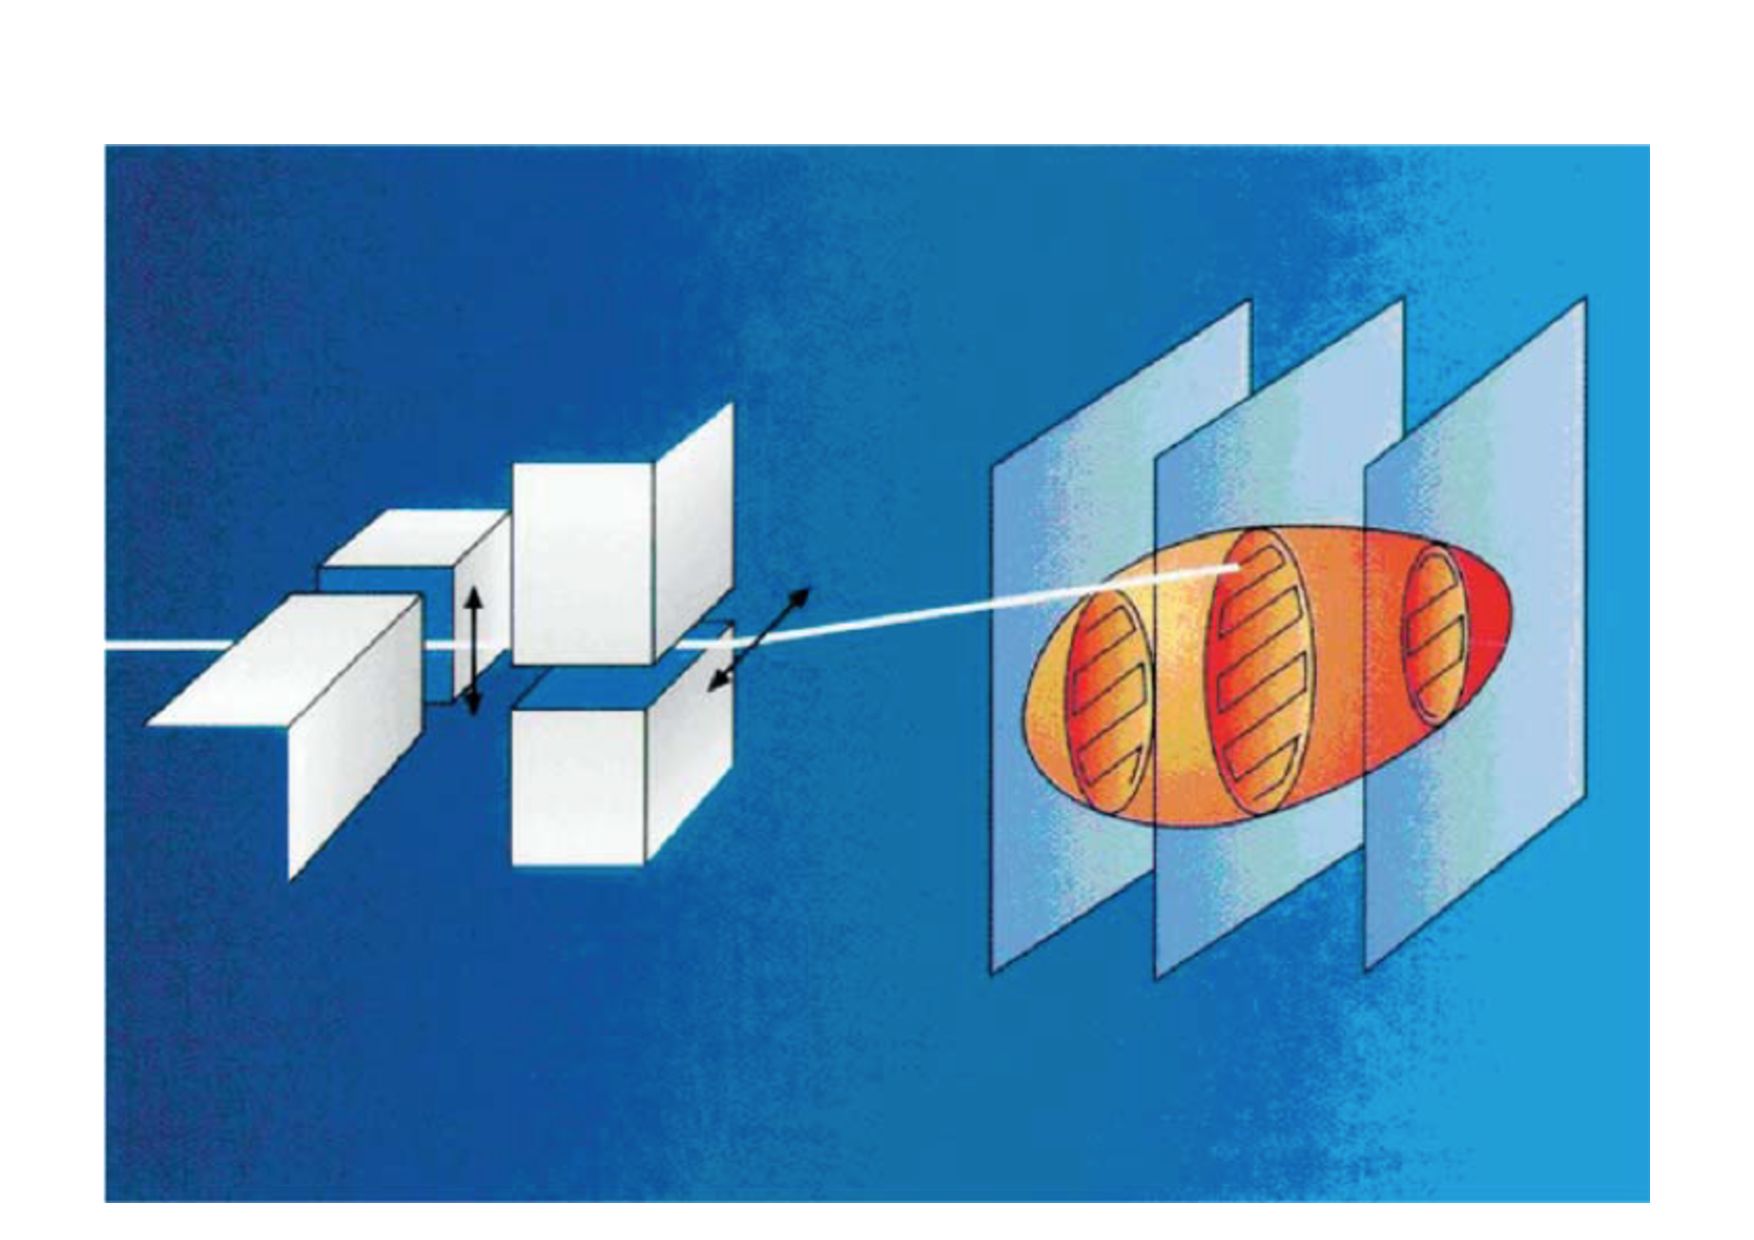
\includegraphics[width=0.7\textwidth]{03_GraphicFiles/chapter1_Introduction/activeDelivery.pdf}
\caption{Schematic view of a fully active beam delivery system. In particular, here the \gls{gsi} raster scanning system is depicted. In~\cite{Schulz-Ertner2006}.}
\label{chap1::fig::activeDelivery}
\end{figure} 

Even if this approach is demanding from the accelerator performance point of view, it brings several advantages with respect to a passive one: there is no need for patient specific equipment like collimators and compensators, and any volume can be in principle covered with a conformal dose; the dose can be adapted on a single voxel basis; the material in the beam line close to the patient is minimized so that the production of secondary particles is strongly reduced. 
With such a delivery system, the term \gls{impt} has been introduced, in analogy to the \gls{imrt} techniques applied in standard photon radiotherapy. Indeed, the \gls{imrt} exploits multi-leaf collimators to tailor the beam to the target, so that it results to be similar to ion passive delivery systems. In photon therapy, the beam modulation on a single spot basis is possible with cyber-knife machines~\parencite{Srivastava2015}.   
The first so-called \enquote{spot-scanning} system was introduced at \gls{nirs}, already in the early 80's~\parencite{Kanai1983}. This first experience was soon followed by a pilot project of spot-scanning at \gls{psi}~\parencite{Pedroni1995} and by the realization of a fully 3D scanning beam system at \gls{gsi}, where the \enquote{raster-scan} technique is implemented~\parencite{Haberer1993} (with the beam moved from one voxel to the next one with no interruptions, and all points in an iso-energy slice connected together in a dense grid). 
Nowadays, various companies are offering commercial scanning beam system solutions, so that a rapid spread of this convenient technique is foreseen for the next years. The counterpart of the active scanning system is a relatively slow delivery of a given dose in a large tumor volume, which can be more rapidly covered by passive delivery approaches.  
 
We described till here static beam configurations, \myMarginnote{Rotating-gantries} with a fixed irradiation position. In the clinical routine, in order to further improve the target volume-to-healthy tissue dose ratio, various beam penetration angles can be foreseen, similarly to standard photon therapy (even if a reduced number of different angles is required). In addition to this, deep-seated tumors close to \glspl{oar} can require specific irradiation angles to be treated with the desired safety margins. In order to achieve this goal, two approaches are possible: rotate the patient or rotate the beam line. 
Even if the patient rotation solution has been explored in the past, several reasons are in favor of a fixed supine position, with only horizontal rotations allowed: the supine position is in compliance with the pre-treatment imaging (\gls{ct} scan) used for treatment planning (see section~\ref{chap1::subsec::treatmentPlan}); a patient rotation necessarily leads to organ motion which is undesired; the supine position is more reproducible in the different treatment fractions. As a consequence, rotating gantries have been developed to allow for the beam line displacement.    
The electron linacs employed in conventional radiotherapy are generally mounted on gantries which can rotate 360 degrees around the patient couch to select the optimum beam direction. 
Likewise, in hadrontherapy, rotating gantries solutions have been designed for both protons and heavier ions. In contrast to the compact gantries used in standard radiotherapy, the high beam magnetic rigidity (defined as the product of the bending radius and the required magnetic field strength, equal to the ratio of momentum to charge of the particles) is a constraint on the size of these structures for proton therapy, and, much more, for heavier ion therapy. In general, the beam is first deflected away from the extraction axis, and then bent back to the patient direction with several dipoles. Moreover, quadrupoles are use to optimize the beam focusing before the treatment room. A scheme of a standard gantry design is given in \figurename~\ref{chap1::fig::schemeGantry}. As already mentioned in section~\ref{chap1::subsubsec::accelerators}, the first gantry for protons was installed at the Loma Linda University Medical Center in 1990, followed in 1996 by the first one in Europe at \gls{psi} in 1996, which also included an upstream scanning system~\parencite{Pedroni1995}. At present most of proton therapy centers are equipped with at least one rotating gantry, generally with passive beam delivery systems.
The huge dimensions imposed by the carbon ion beam rigidity (three times bigger rigidity for 5000~MeV carbon ions with respect to 200~MeV protons) limited the implementation of such a technology in carbon therapy centers, while different technical solutions have been explored. As an example, at \gls{himac}, in a single treatment room the beam can be delivered to the patient via an horizontal and a vertical line, for the sequential treatment from different angles. The first rotating gantry system for heavy ions was installed at \gls{hit} and is now in operation: the diameter is of 13~m, for a total weight of about 700 tons (see \figurename~\ref{chap1::fig::HITgantry}).

 \begin{figure}[!htbp]
 \begin{subfigure}[t]{.49\textwidth}
\centering
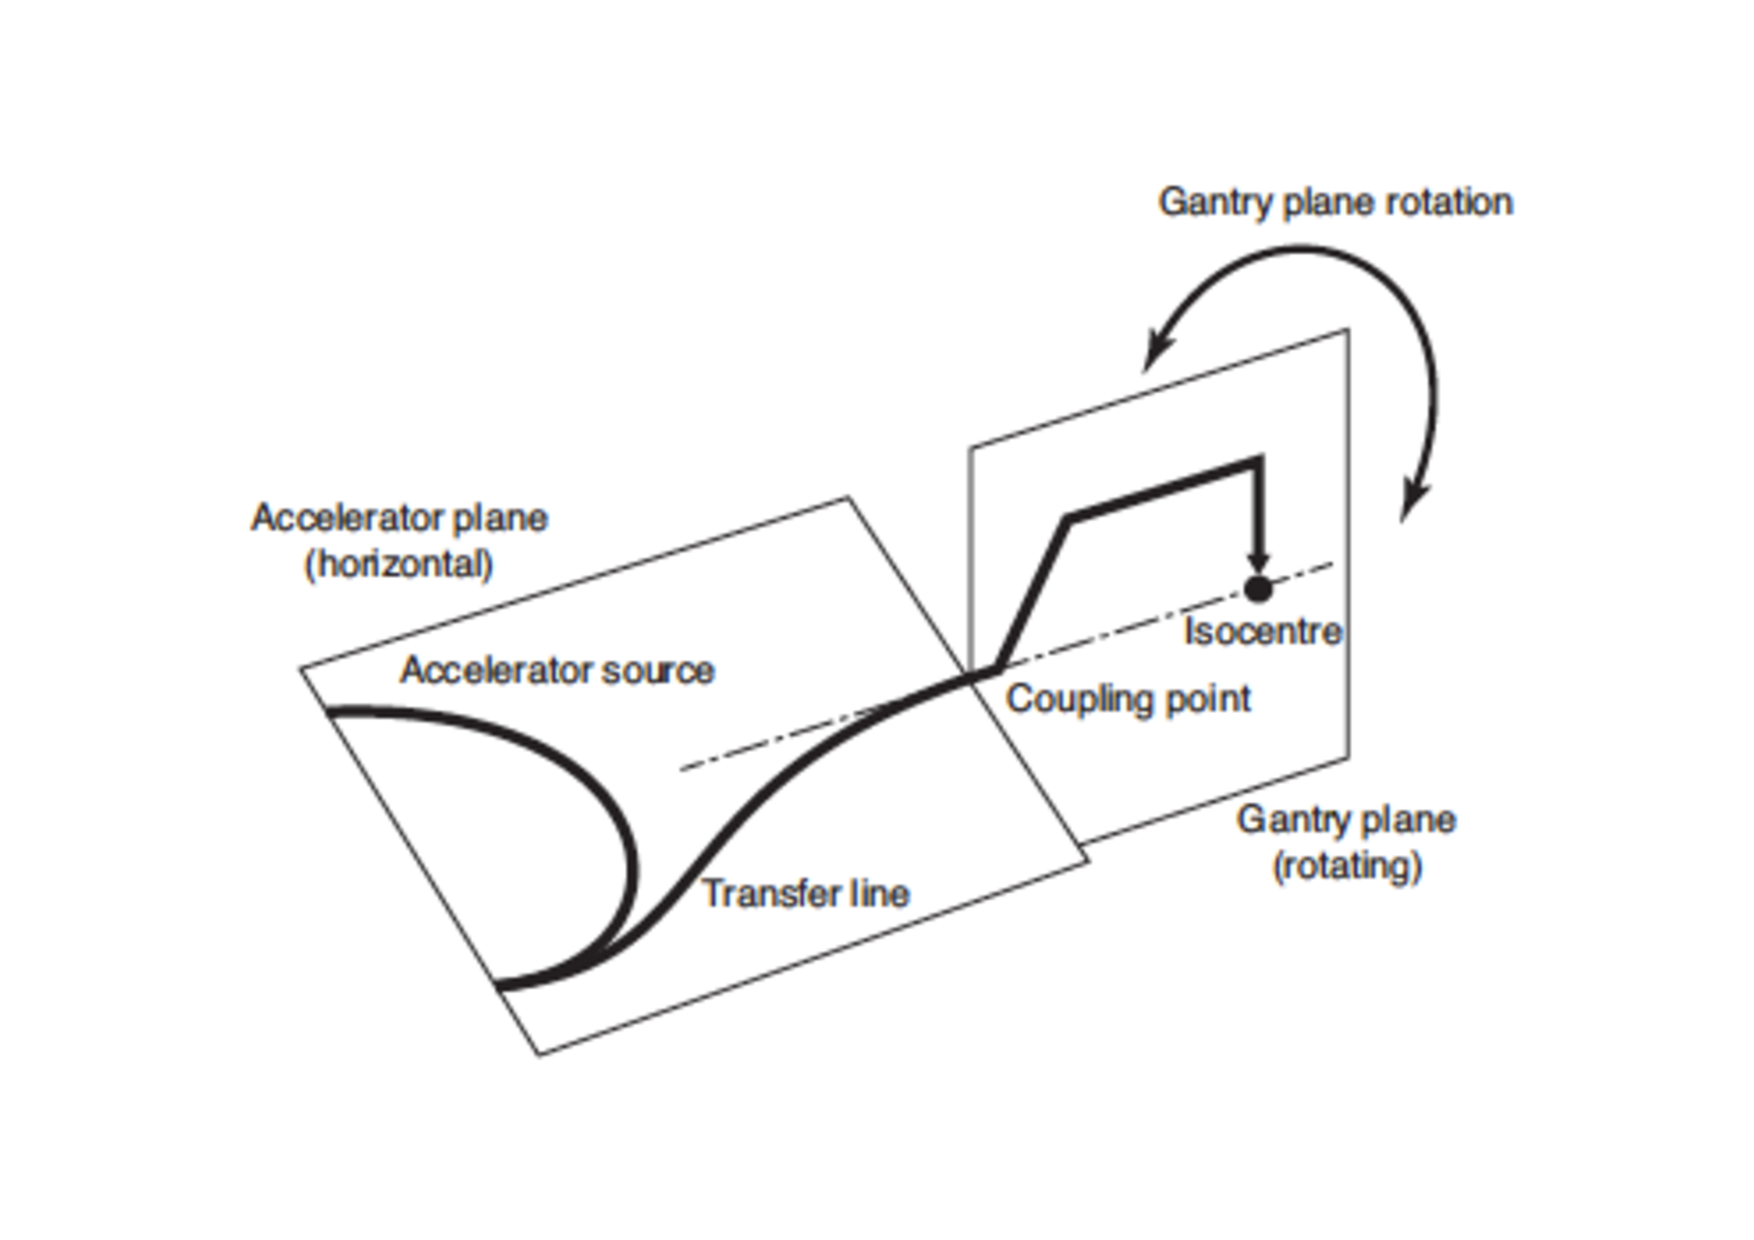
\includegraphics[width=0.92\linewidth]{03_GraphicFiles/chapter1_Introduction/scheme_gantry.pdf}	
\caption{Schematic design of a rotating gantry installed in a particle therapy center. In~\cite{Owen2014}.}
\label{chap1::fig::schemeGantry}
\end{subfigure}
 \begin{subfigure}[t]{.49\textwidth}
\centering
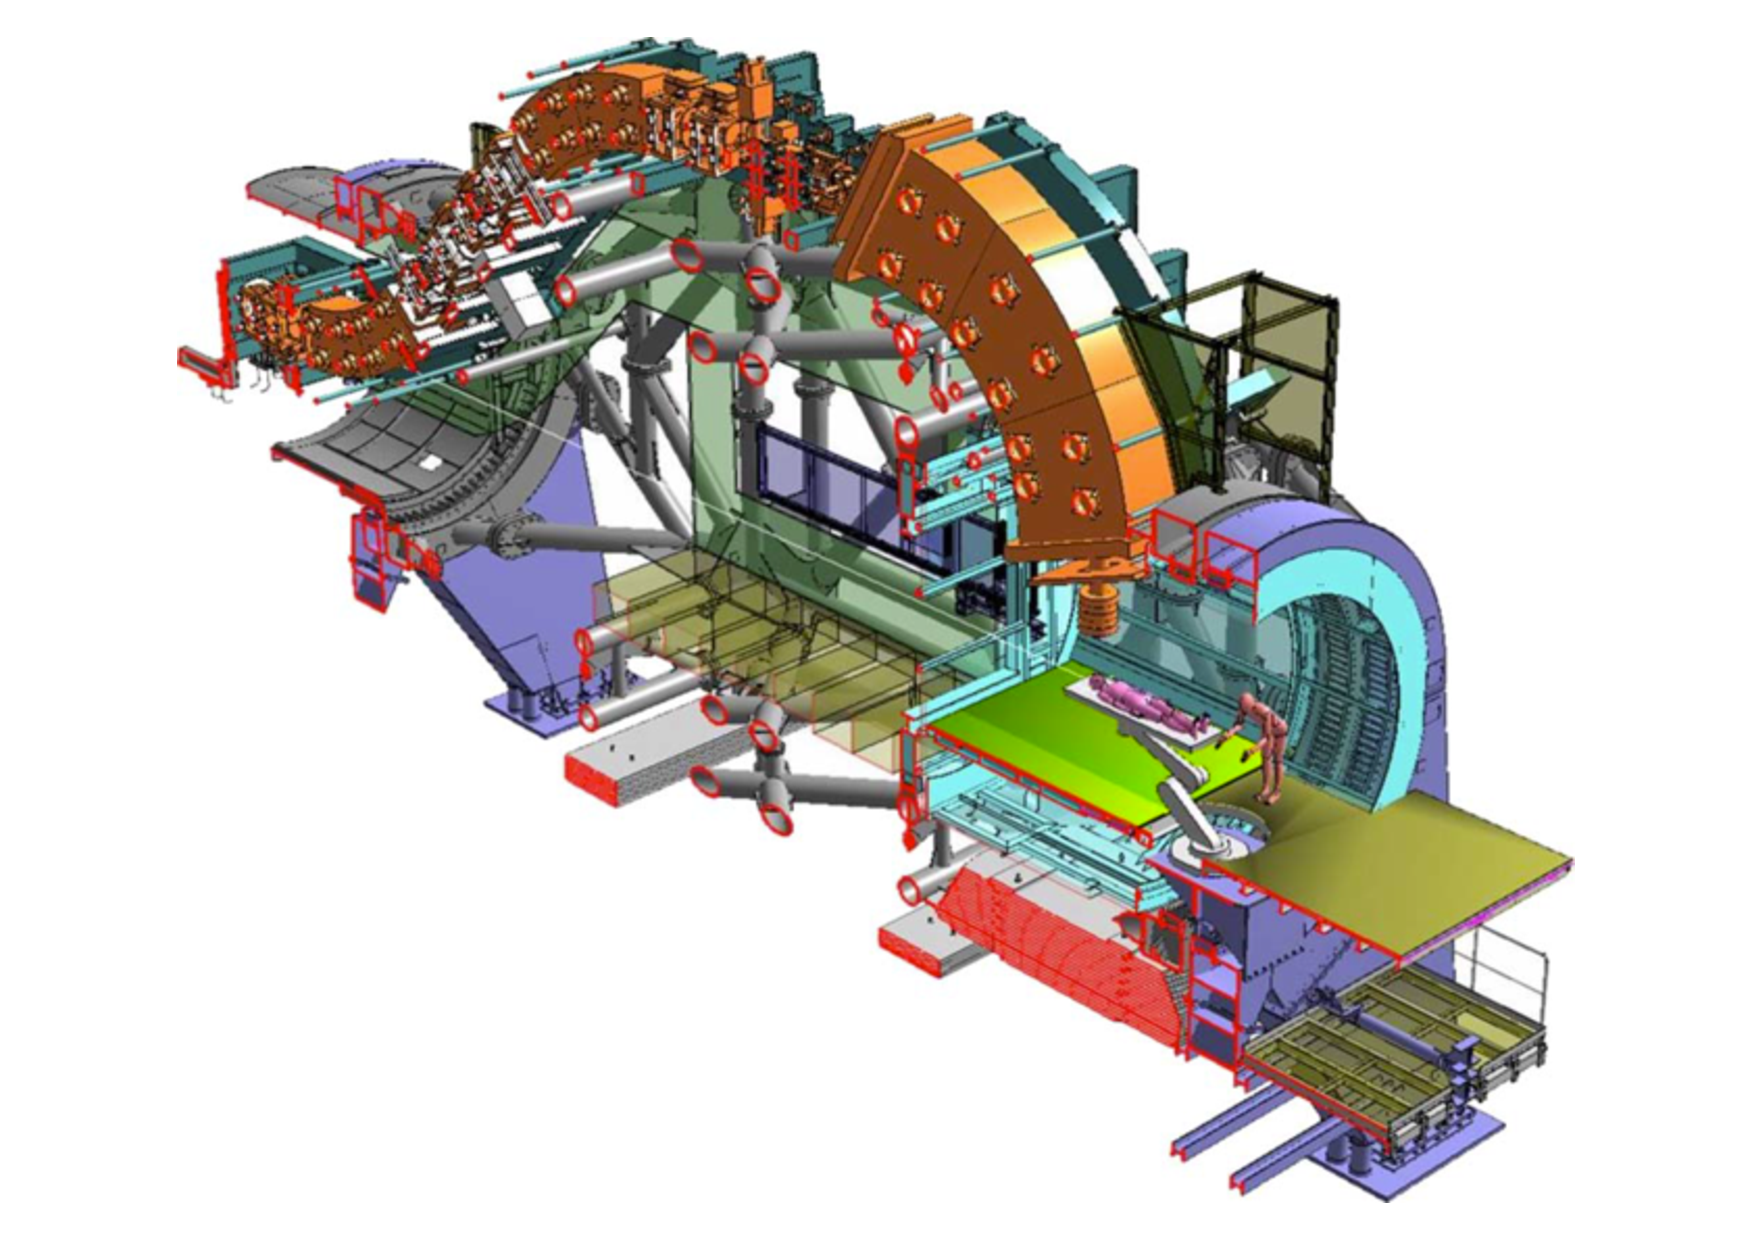
\includegraphics[width=0.99\linewidth]{03_GraphicFiles/chapter1_Introduction/HITgantry.pdf}
\caption{Scheme of the \gls{hit} ion rotating gantry. In~\cite{Schardt2010}.}
\label{chap1::fig::HITgantry}
\end{subfigure}
\caption{Schemes of a standard gantry design (left) and of the carbon-ion rotating gantry installed at \gls{hit} (right).}
\label{chap1::fig::Gantry}
\end{figure}           

Intense research efforts are dedicated to improve the gantry technology, mainly directed towards the implementation of more compact systems equipped with superconducting magnets. A first superconducting carbon ion gantry has been recently installed at \gls{nirs}, and is approximately half size with respect to the German one~\parencite{Iwata2013}.

\subsection{Treatment planning}\label{chap1::subsec::treatmentPlan}

Given the available accelerator and beam delivery system, the best possible treatment features are elaborated by the treatment planning process, which combines the clinical information about the patient with the physical an biological aspects of particle therapy. 
The treatment planning is always patient and disease-specific, and is based on imaging techniques aiming to provide the physicians with the data necessary to delineate the target volume and the surrounding \glspl{oar}. The minimal approach is represented by a pre-treatment x-ray \gls{ct} scan, providing quantitative information about the anatomical structures via photon attenuation images. As briefly outlined in the previous paragraph, it is important to record the pre-treatment images in the same conditions (patient position, fixation structures, etc.) later applied in the treatment itself. Complementary imaging devices, such as \gls{mri} and \gls{pet}~\parencite{Levy2007}, are often used in combination with \gls{ct} to improve the target definition quality, mainly in case of proximity with \glspl{oar}.
In addition to the target delineation, the physicians are also in charge of the therapy prescription, which includes the total dose to be delivered to the \gls{ptv}, the dose limits for the surrounding tissues, and the fraction planning.
All the listed information are the input for the \gls{tps} \myMarginnote{Treatment-Planning System}, which makes the connection between the prescribed dose distribution and the beam acceleration and delivery devices. The physicists and clinicians use the \gls{tps} to define all the treatment beam-specific features such that the clinical prescription is satisfied at the maximum extent. The software output details the beam entrance ports to be used (in terms of gantry positions, if a gantry is available), the beam ranges and intensities, the irradiation scheme in terms of dose-per-voxel, and, more generally, the expected dose distribution in the patient, which allows to quantify the ~\gls{tcpr} and the probability of complications to
the normal tissues.
As the whole planning process is based on x-ray \gls{ct} scans,  \myMarginnote{From Hounsfield units to relative stopping power} providing photon beam attenuation images, a relationship between the \gls{ct} values and ion~\gls{rsp} is needed. The \gls{ct} values are expressed in \gls{hu}, defined as

\begin{equation}
\mathrm{CT\,value}(\vec{x}) =1000 \times \frac{\mu (\vec{x})-\mu_{W}}{\mu_{W}}
\label{chap1::eq::HU}
\end{equation}
where $\vec{x}$ is the considered location, $\mu(\vec{x})$ the x-ray absorption coefficient in tissue, $\mu_{W}$ the one in water as reference. Water is always used as reference medium, in particular through the concept of \gls{wepl}. There is not a functional relationship between the two quantities, and systematic studies have been carried out at \gls{psi} for protons~\parencite{Schneider1996, Schaffner1998}. For carbon ions, similar investigtions have been performed at \gls{nirs}~\parencite{Matsufuji1998, Kanematsu2003} and \gls{gsi}~\parencite{Jakel2001, Rietzel2007}, and experimental verification has been obtained via measurements on animal tissues. In \figurename~\ref{chap1::fig::HU} the data of a look-up table for the conversion of \gls{hu} into carbon ion \gls{wepl} are plotted in the \gls{hu} range of relevant biological tissues.

 \begin{figure}[!htbp]
 \begin{subfigure}[t]{.49\textwidth}
\centering
\includegraphics[width=0.92\linewidth]{03_GraphicFiles/chapter1_Introduction/HounsfieldUnits.pdf}	
\caption{Hounsfield look-up table for carbon ion treatment planning, based on the data collected at \gls{gsi} and reported in~\cite{Jakel2001}. In~\cite{Rietzel2007}.}
\label{chap1::fig::HU}
\end{subfigure}
 \begin{subfigure}[t]{.49\textwidth}
\centering
%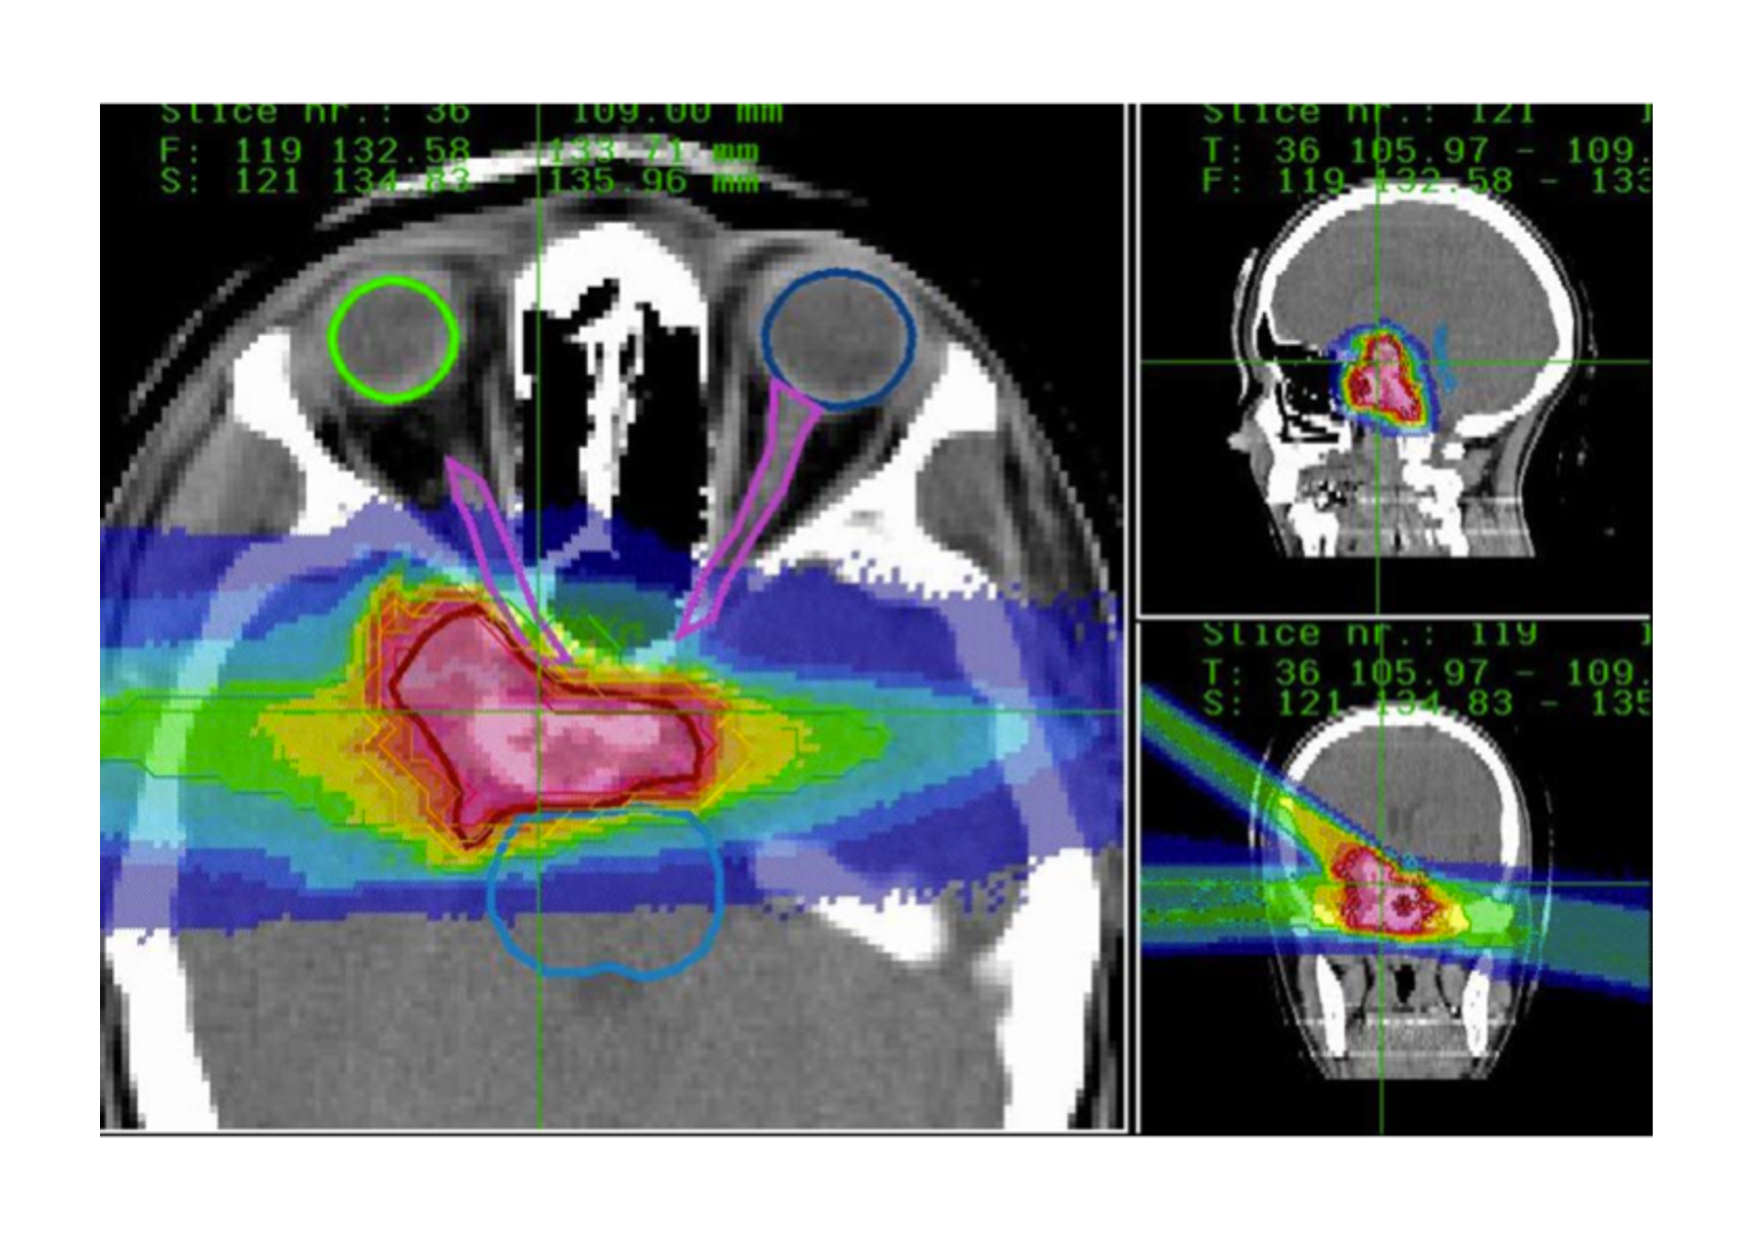
\includegraphics[width=0.92\linewidth]{03_GraphicFiles/chapter1_Introduction/TRIPplan.pdf}
%\caption{Biologically effective dose distribution for the treatment of a skull base tumor, optimized with the \gls{tps} TRiP~\parencite{Kramer2000} at \gls{gsi}. In~\cite{Schardt2010}.}
%\label{chap1::fig::tps_plan}
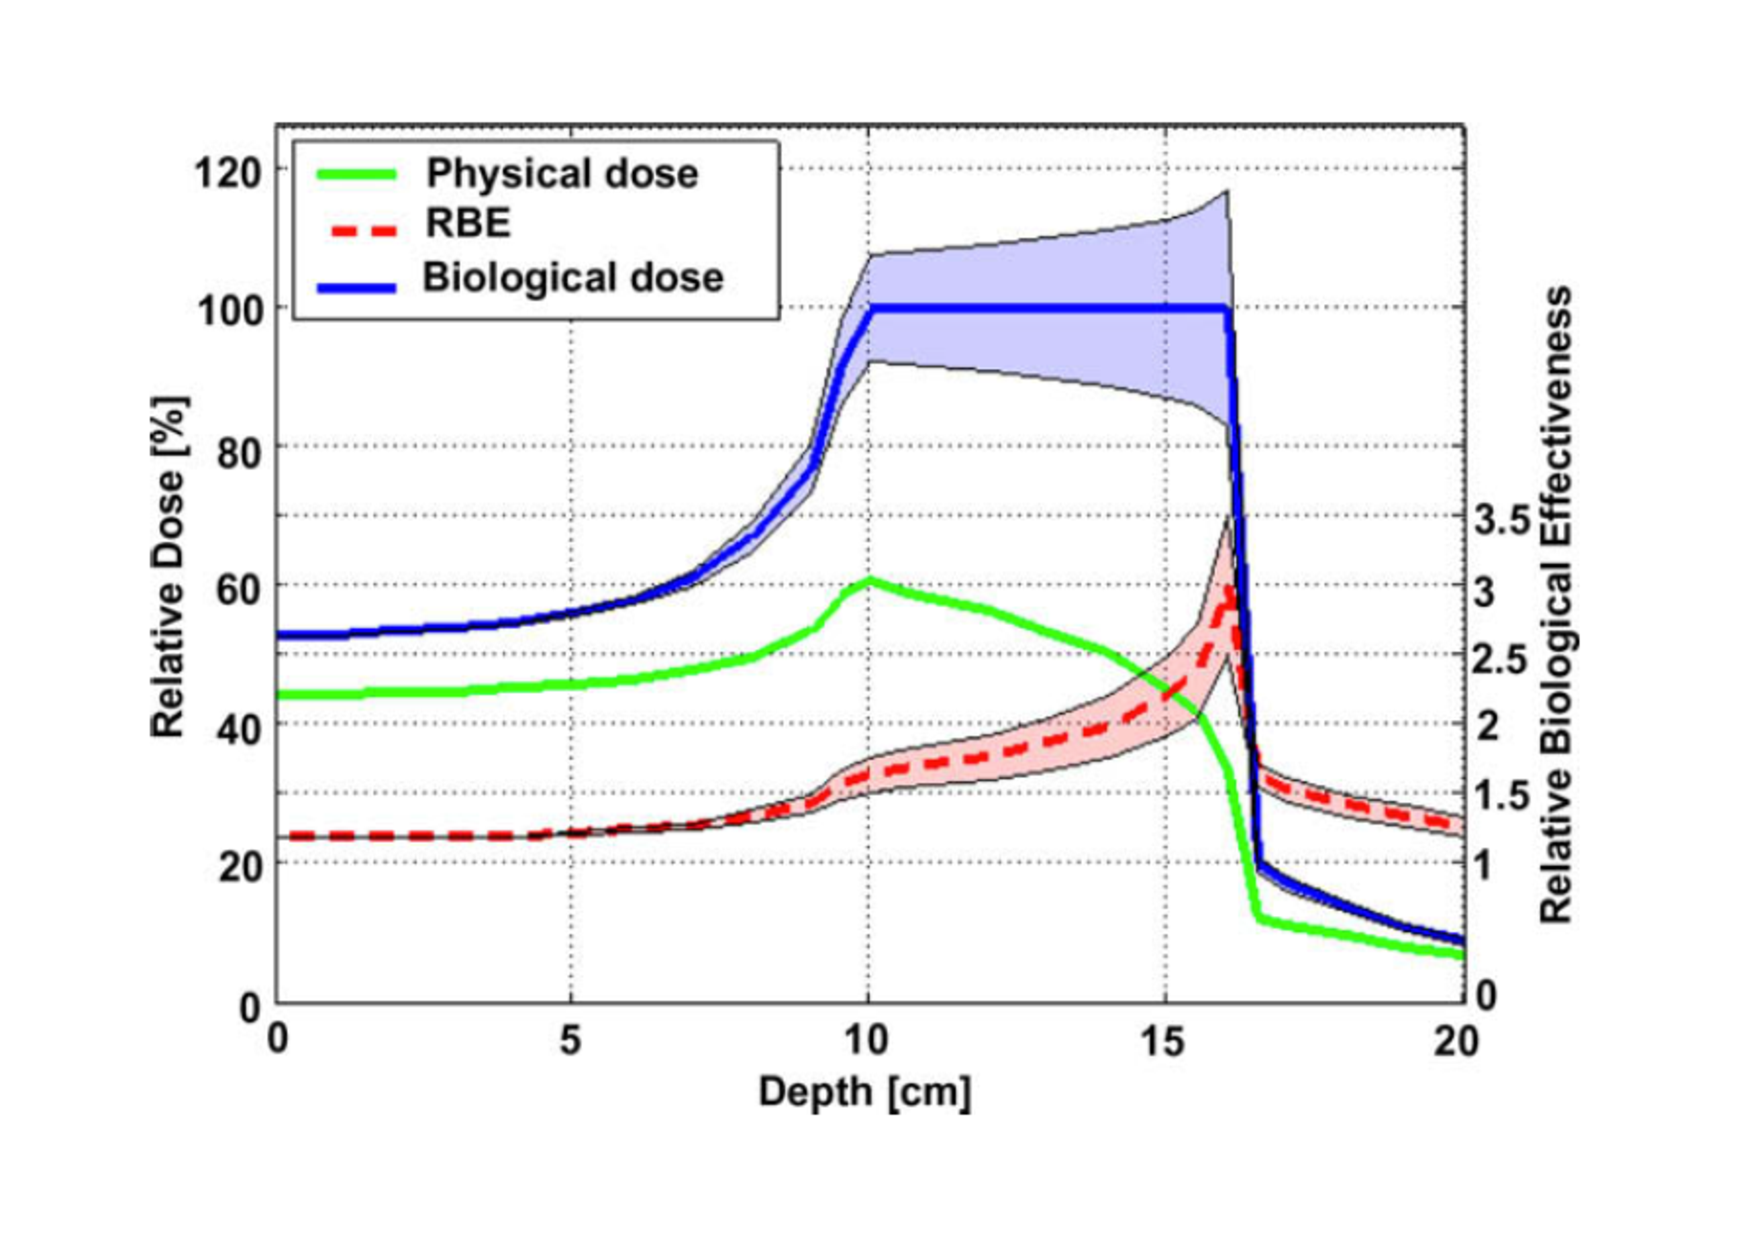
\includegraphics[width=0.92\linewidth]{03_GraphicFiles/chapter1_Introduction/rbeWeightedDose.pdf}
\caption{Comparison of physical (green solid line) and biological (blue solid line) dose for a 290~MeV $^{12}$C ion beam with a 6 cm SOBP for an assumed maximum \gls{rbe} of 3.0. The \gls{rbe} varies in the range 2.5–3.5 and an uncertainty band is sketched to represent the biological dose possible variation due to the selection of the \gls{rbe} value (dashed-red line). In~\cite{Suit2010}.}
\label{chap1::fig::rbeDose}
\end{subfigure}
\caption{The treatment planning system process is based on anatomical information about the patient, given by \gls{ct} scans, and physician treatment prescription. The \gls{ct} values must be converted to \gls{rsp} and tabulated experimental data are used (left), while biological dose calculation models are applied to optimize the biological dose distribution to be delivered during the treatment (right), with the related uncertainties connected to the \gls{rbe} variations.}
\label{chap1::fig::TPS}
\end{figure}           

The conversion factors are tabulated and implemented in the main \glspl{tps}, but several studies are still ongoing in order to optimize the calibration accuracy (as an example, see~\cite{Inaniwa2018}). As highlighted in several research works, this is one of the main sources of uncertainty affecting proton and carbon ion range prediction and, so, treatment precision. Possible investigated solutions to reduce systematic uncertainties in the \gls{rsp} determination related to the Hounsfield unit conversion are represented by \gls{pct} and dual energy x-ray \gls{ct}~\parencite{Yang2010}. Further details will be given in section~\ref{chap1::subsec::uncertainty}.
In addition to the beam range determination, \myMarginnote{Biological dose modeling} the \gls{tps} software must also deal with biological dose calculations. Indeed, as highlighted in section~\ref{chap1::subsec::bioEffects}, charged particles differ from photons in their radiobiological properties and effects. Notwithstanding the 10-20\% \gls{rbe} variations verified for protons with varying \gls{let} along the path in the patient tissues, a practical constant value of 1.1 is generally used in clinics~\parencite{Paganetti2002, ICRU2007}. This value corresponds to the average \gls{rbe} at mid \gls{sobp} overall dose levels. In the distal section of the Bragg peak, an higher \gls{rbe} has been verified; this effect slightly affects the dose profile fall-off in protontherapy and is not modeled in the present planning systems. As mentioned in section~\ref{chap1::subsec::bioEffects}, several studies are ongoing in the last years with the aim of optimizing the biological models and applying a variable proton \gls{rbe} in clinics, and the topic is still open to discussion in the expert community~\parencite{Paganetti2013, Paganetti2014, Unkelbach2018, Luhr2018, Willers2018}. A different approach must be applied to heavy ions (carbon ions in particular), given the much stronger dependence of their \gls{rbe} on the various parameters listed in section~\ref{chap1::subsec::bioEffects}. Focusing on carbon ions, treatment plans are generally optimized using the so-called \gls{rbe}-weighted dose, calculated according to verified models based on experimental data. In \figurename~\ref{chap1::fig::rbeDose}, the physical and biological doses absorbed during a carbon ion beam irradiation with a \gls{sobp} are compared and the \gls{rbe} variation along the beam path is also reported, together with the estimated uncertainties which also affect the \gls{rbe}-weighted dose evaluation. For this purpose, two main models are nowadays implemented in clinical practice. On one side, the Japanese centers use a model developed at \gls{nirs}, based on in vitro cell killing experiments on human salivary glands and neutron irradiation experience gathered at \gls{himac}, as well as on the application of the \gls{lq} model~\parencite{Matsufuji2007}. Recently, a modified \gls{mkm} has been introduced in order to optimize the plans to active scanning with ion beams~\parencite{Inaniwa2015}. On the other side, a specific biophysical model has been developed in Germany at \gls{gsi}, called \gls{lem}, and it is now used in the clinical centers in Germany, Italy and China. Its main idea is to transfer known cell-survival data for photons to ions, assuming that the difference in biological efficiency arises only from a different pattern of local dose deposition along the primary beam~\parencite{Kramer2000, Jakel2001a}.
The two models have been verified to give comparable results, in agreement with the measured \gls{rbe}, with in-vitro experiments on mice cells~\parencite{Uzawa2009}, while different predictions are obtained when different treatment schemes on different tissues are studied~\parencite{Fossati2012, Steinstrater2012}. Besides, the NanOx model (described in ~\cite{Cunha2017}) is being developed in order to overcome conceptual inconsistencies of the \gls{lem} and \gls{mkm}. The model is able to predict cell survival with good agreement to experimental data, and its parameters are under study for optimization~\parencite{Monini2018}. The definition of a common effective dose prediction method is ongoing: this will allow for comparative studies of clinical results and for an improved collaboration of the few ion treatment centers operating all over the world.
These biological models are mainly applied for the planning of active scanning treatments, for which the target volume is previously divided into slices: the dose is then optimized for iso-range slices. In contrast, for passive beam delivery systems, the plan optimization is generally reduced to the study and production of the patient-specific beam modulators. 
In the future, biology-guided forms of particle therapy can be foreseen; the \gls{rbe} variations, instead of being an issue for which corrections are needed to the treatment planning, could be used to the treatment effectiveness advantage.  
Focusing on the possible direction of improvements in the future of treatment planning \myMarginnote{Treatment of moving organs}, the research efforts are concentrated in the last years also on another fundamental topic: the treatment of moving organs. It is clear that the well-defined ion range and narrow dose peak make ion treatments potentially more sensitive to inter- and intra-fractional organ motion, as highlighted in~\cite{Phillips1992, Bert2008, Engelsman2013} and~\cite{Thornqvist2013}, as an example. Concerning the organ displacement between following fractions, it can be corrected by more frequent imaging scans, ideally a new one before every treatment fraction, in order to adapt the treatment planning to weight variations, target size modifications and similar anatomical effects. The organ movement caused by the respiratory cycle requires more complex strategies to be taken into account for the treatment plan and delivery. The respiratory motion patterns are genarally complex and not regular, involving translational and rotational displacements. Several strategies to mitigate the effect of organ motion are being investigated, some of them directly coming from the experience gathered in \gls{imrt}. As well summarized in~\cite{Schardt2010}, among these strategies it is worth to mention rescanning of repainting techniques, based on the average effect of several irradiations with reduced beam fluence on the same iso-range slices; gating techniques, which aim to correlate the irradiation active time to a continuous monitoring of the respiration cycle; tracking, which requires a 3D compensation of the target motion in real-time, particularly adapted for scanning techniques. A further step will be the real time monitoring of moving organs by means of external markers linked to biomechanical modelling of internal organs~\parencite{Manescu2013}. Some of the cited techniques, or combinations of them, are being tested and are now at the validation stage, but there is still wide room for improvements towards the application of 4D treatment planning~\parencite{Graeff2013, Bert2017}. Further information about this topic  can be found in a recent review by Kubiak~\parencite{Kubiak2016}.    
Range predictions, biological modeling and organ motion are only some of the sources of uncertainties affecting the planning and delivery of ion therapy treatment, detailed in section~\ref{chap1::subsec::uncertainty}; for this reason, safety margins \myMarginnote{Safety margins} are applied in clinics for the definition of the irradiation target volume and the quantification of the planned dose. In the actual clinical routine, the \gls{ptv} is a geometrical extension of the so-called \gls{ctv} and is delineated in order to account for treatment uncertainties. Safety margins are also applied in standard x-ray therapy~\parencite{McKenzie2000}, where under- or over-shooting errors have limited effects with respect to ion beam therapy. As highlighted in~\cite{Albertini2011}, the application of safety margins is useful to improve the treatment plan robusteness in case low dose gradients are applied, while the effect results marginal for highly modulated \gls{impt}. At present, in order to account for the overall effects of all sources of uncertainties in the range prediction (\gls{mcs}, beam energy straggling, imaging tools accuracy and calibration, biological effects, patient positioning and organ motions), margins up to 3.5\% + 3~mm can be applied around the \gls{ctv}~\parencite{Paganetti2012}, mainly based on Monte Carlo or analytical dose calculations which result in clinically compatible predictions. 

In the following paragraph, the uncertainties related to ion therapy treatment are discussed in details, with particular care devoted to possible clinical solutions.

\subsection{Ion beam therapy uncertainties and treatment monitoring}\label{chap1::subsec::uncertainty}
Heavy charged particles are suitable for cancer radiation therapy given the better achievable dose conformity and the reduced energy deposit in tissues surrounding the target with respect to standard photon treatment techniques. These advantageous features directly derive from the nature of ion interactions in matter, described in section~\ref{chap1::subsec::Physics}, which determines a peculiar depth dose profile characterized by a finite range and a energy deposit (dose) peak (Bragg peak). In order to accurately predict the ion range and, more generally, the dose distribution delivered during a clinical treatment, all the possible ion interactions in matter must be considered. This prediction is associated with considerable uncertainties due to imaging precision, patient setup, anatomical variations and motions, beam delivery system accuracy, dose calculation approximations and biological considerations~\parencite{Paganetti2012}. Ideally speaking, a perfect knowledge of the beam and target structure and perfect evaluation of all the parameters involved in the dose determination would result in the optimal way to treat a deep-seated tumor, with a reduced dose delivered to the surrounding healthy tissue (even close to \glspl{oar}) with limited fields of irradiation, and a dose accurately concentrated to the tumor volume. The actual clinical routine must face limitations in beam production and control as well as in patient composition evaluation, which causes the need for approximated treatment planning and the setup of treatment safety margins (see section~\ref{chap1::subsec::treatmentPlan}), limiting the full exploitation of this treatment technique potential. In this section, an overview of the different sources of uncertainties affecting ion therapy treatments is given, and the solutions, already implemented or under study, are presented, with particular attention focused on ion range monitoring techniques, main topic for this thesis.
All the mentioned sources of uncertainties associated to hadrontherapy treatment converge in a considerable spread in the beam effective range with respect to the predicted one. Treatment planning systems are able to accurately model range straggling and \gls{mcs} broadening along the beam path in water~\parencite{Hong1996}, but the prediction accuracy has limitations when translated to patients. As highlighted in~\cite{Schlegel2008}, a precise determination of the primary ion penetration depth is essential in order to rely on particle therapy treatments, much more than for standard photon treatments. The reason is schematically presented in \figurename~\ref{chap1::fig::rangeUnc}.

\begin{figure}[!htbp]
\centering
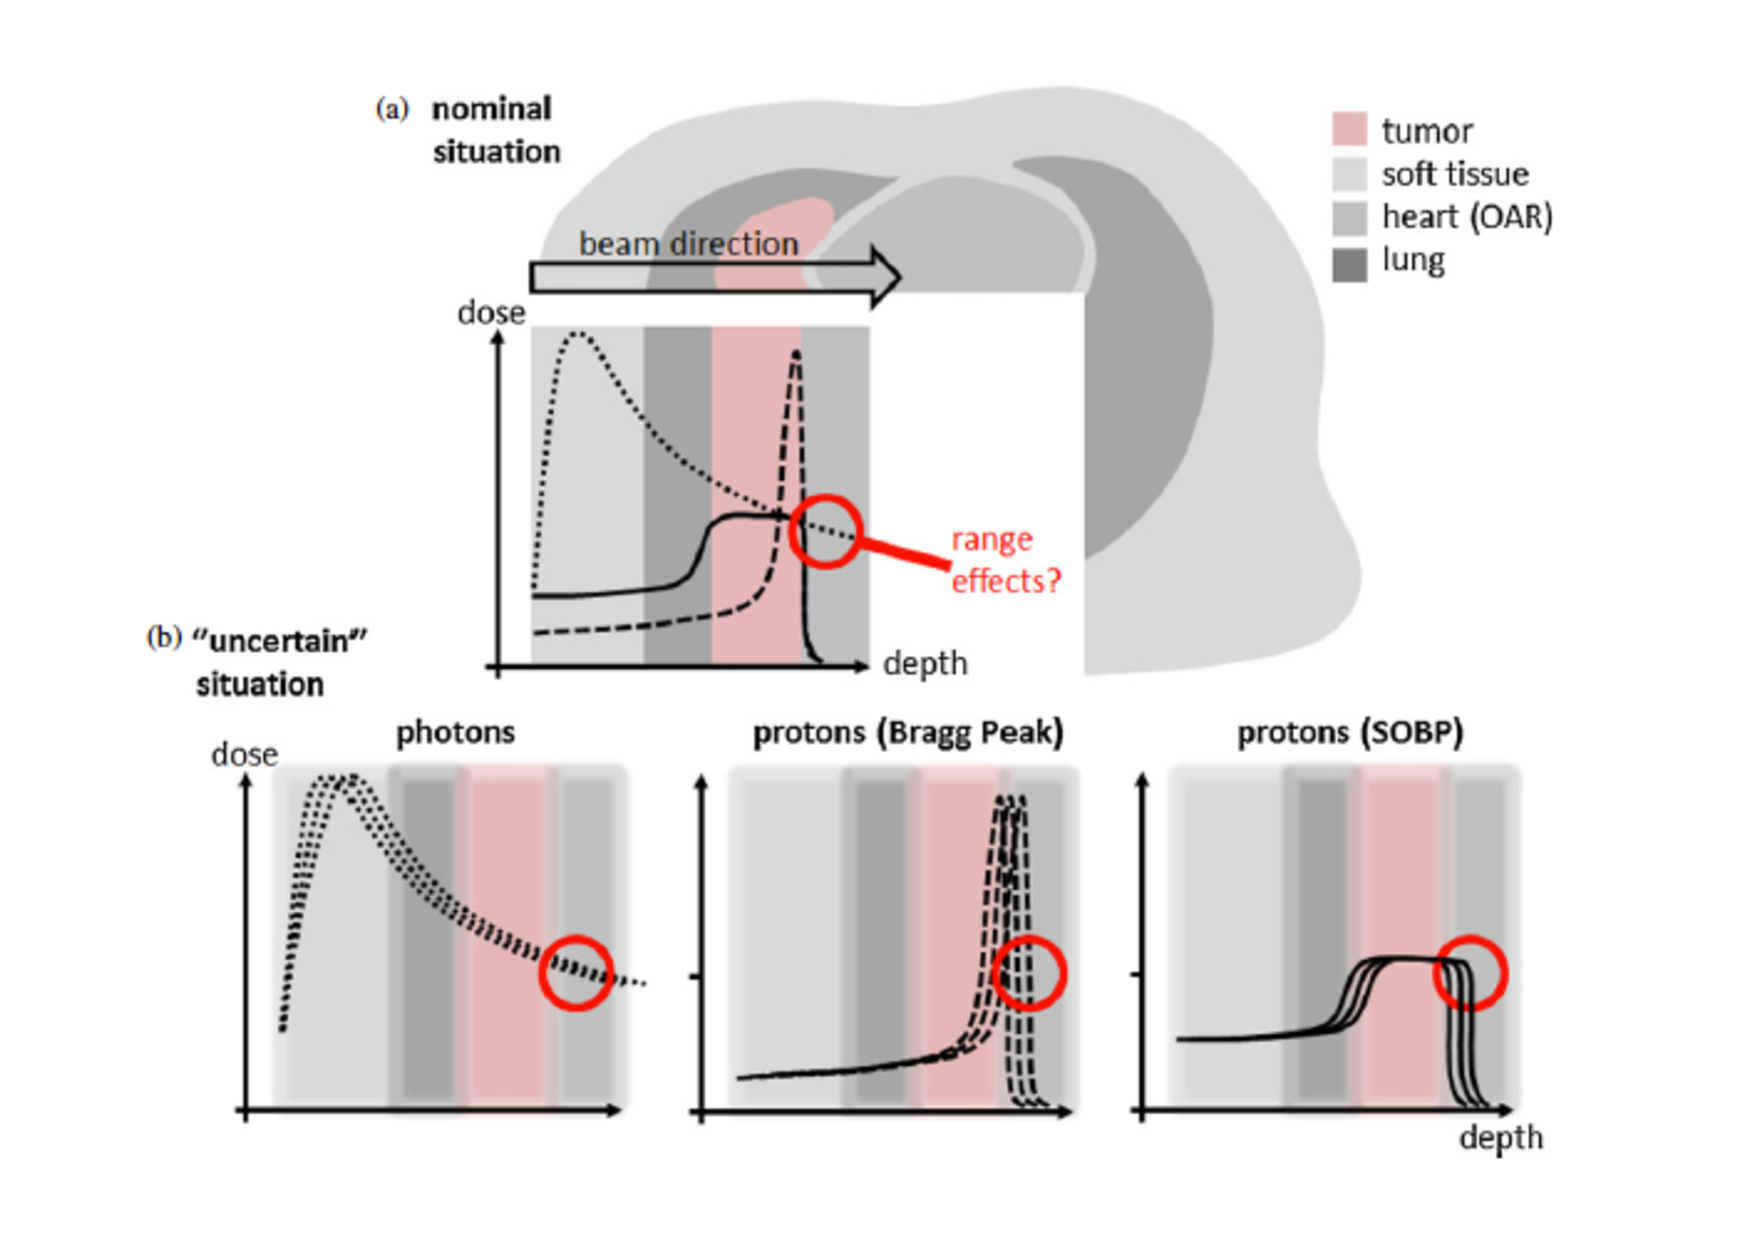
\includegraphics[width=0.7\textwidth]{03_GraphicFiles/chapter1_Introduction/rangeUnc.pdf}
\caption{Schematic view of the potential benefit due to the depth-dose features of protons as compared to photons (a) and influence of range uncertainties on photon irradiation and proton pristine and spread-out Bragg peaks. In~\cite{Knopf2013}.}
\label{chap1::fig::rangeUnc}
\end{figure} 

In the top panel of \figurename~\ref{chap1::fig::rangeUnc} the ideal treatment configuration is shown, with the pristine Bragg peak located at the distal limit of the \gls{ptv} (dashed line) and the \gls{sobp} covering the whole tumor volume (solid line); the two proton irradiation methods are compared to the photon dose profile (dotted line), which releases the maximum of the dose in the entrance region and it is not capable of sparing the tissues surrounding the tumor volume, before and beyond the tumor in the beam direction. In the bottom line of the same figure, the effect of range uncertainties are represented: from left to right, in case of photon dose profile shifts, the modification in the dose delivered to healthy tissues is relatively limited, the main effect being a shift in the dose maximum in the entrance region; for a monoenergetic Bragg peak, a shift in the peak position can result in both an under-irradiation of malignant tissues and a dose maximum located in soft healthy tissues; the same effect is present for the \gls{sobp}, with the only advantage of a reduced under-irradiation of the tumor region. It is clear from this simple case how the extremely sharp dose gradient provided by heavy charged particles must be accurately controlled in order to fully profit of its beneficial effect in treating cancer. 
As mentioned, an exact range calculation is extremely difficult to be obtained in human tissues. As described in section~\ref{chap1::subsec::treatmentPlan}, the treatment planning is at present based on a pre-treatment \gls{ct} scan which is generally acquired only before the first treatment fraction. The \gls{ct} image accuracy is indeed the first source of uncertainty in range calculation \myMarginnote{\gls{ct} uncertainty}. The limitations in the imaging precision (mainly due to image noise - see~\cite{Chvetsov2010}) and the reconstruction artifacts (which can be relevant in presence of metal implants as verified in~\cite{Jakel2007, Newhauser2007}) already affect the reference data set. Small but not negligible effects are also related to the \gls{ct} resolution~\parencite{Espana2011}. The obtained \gls{ct} data must be then converted from x-ray attenuation values (\gls{hu}) related to water to relative ion stopping power (see section~\ref{chap1::subsec::treatmentPlan}). The conversion is based on calibration curves~\parencite{Schneider1996, Schneider2000}, generally obtained with \gls{ct} scans of tissue phantom materials with known density and elemental composition. These curves are affected by uncertainties, to be added to the fact that the actual conversion is dependent on the material composition: same x-ray attenuation values can correspond to different relative stopping powers, or vice versa. In addition to this, the conversion may depend on the specific \gls{ct} scanner, as shown in~\cite{Ainsley2014}. Several studies have highlighted the magnitude of such uncertainties, which varies, for example, in the range 1-2\% from soft tissues to bones for protons~\parencite{Schaffner1998b}, which is translated in range possible discrepancies of 1-3~mm. Specific studies have also been conducted on animal fresh tissues in order to otpimize the \gls{ct} calibration for carbon ion treatments~\parencite{Rietzel2007}. In total, uncertainties of the order of 3\% are generally considered to take into account the described imaging limitations~\parencite{Moyers2001}. It has been proven that dual-energy \gls{ct} can improve material composition information~\parencite{Bazalova2008, Yang2010, Hunemor2014, Wohlfahrt2018} and the resulting range uncertainties can be reduced, in particular for carbon ion therapy~\parencite{Hunemor2014}. A possible solution to further reduce the errors related to the \gls{hu} values conversion is the implementation of direct density measurements techniques, where the treatment beam is also used for imaging purposes giving direct access to stopping power data. This possibility was discussed since the late sixties~\parencite{Koehler1968}, and the technological advancements (mainly in data acquisition systems and detection techniques) recently allowed to obtain promising results in the last years. In addition to the advantageous removal of the data conversion stage, the so-called ion radiography brings other benefits to the treatment side, with the possibility of performing position verification with fast scans just before the treatment delivery~\parencite{Schneider1995}, as well as on the patient side, given the reduced dose necessary for a complete scan with respect to standard x-ray \gls{ct}~\parencite{Schneider1995}. Further details about this imaging technique are given in the dedicated section~\ref{chap1::subsubsec::particleCT}.
Till here the uncertainties directly coming from the treatment planning process have been described, and can be considered as systematic errors, reproduced unchanged for every delivered fraction of the treatment. Conversely, stochastic uncertainties emerge at the treatment delivery level and affect the planned range with random variations. The majority of treatment planning system operating in clinics are based on analytical calculations relying on \gls{wepl} data, not able to account for complex geometries. In presence of tissue inhomogeneities \myMarginnote{\gls{mcs} range degradation}, \gls{mcs} causes what is generally referred to as a degradation in the distal fall-off of Bragg peaks~\parencite{Urie1986}, in particular in proximity of high-density gradients.  Accurate modeling of \gls{mcs} is then strictly required for correct range predictions~\parencite{Schuemann2014}. The patient anatomical configuration\myMarginnote{Patient anatomy changes} plays a major role not only on a single fraction basis, but also in different fractions. Conventional fractionation schemes foresee treatments which can last for several weeks; the patient anatomical characteristics can experience significant changes, such as tumor mass reduction, weight loss or gain~\parencite{Albertini2008}, modifications in the filling of internal cavities. It is clear that such variations introduce further shifts in the predicted ion range, which can be different from fraction to fraction. Moreover, in different fractions, slight differences in the delivered ion energy are possible, with small but not negligible effects. 
Moving on but always referring to static anatomy issues, the patient setup in the treatment room is another source of uncertainty which can cause discrepancies between the planned and the delivered dose distribution, as shown for example in~\cite{Fattori2014}. 
Furthermore, in particular for the treatment of tumors in the thorax, organ motion \myMarginnote{Organ motion dose blurring} is an important source of dose delivery errors. Focusing on lung cancers, which are already difficult to be precisely targeted due to the low lung density (3 times lower than water), the respiratory motions are hard to be modeled and cause an overall blurring of the dose distribution and severe local range variations due to the high-density gradient between dense tumor tissues and low-density lung tissue. Important research efforts are devoted to the optimization of the treatment of moving organs, as explained in section~\ref{chap1::subsec::treatmentPlan}. In particular, for active scanning delivery techniques, potentially powerful if synchronized with the movements of the target areas, an interplay effect involving beam and organ motion can affect the dose homogeneity and must be minimized~\parencite{Dowdell2013, Grassberger2015}.
To conclude the list of source of uncertainties affecting ion beam therapy treatment planning and delivery, it is worth to mention the contribution of biological effects \myMarginnote{Biological effects}. For protons, a generic constant \gls{rbe} value is generally used in clinics to relate proton dose to photon dose, while it has been verified how the biological effectiveness varies along the beam path, in particular at varying \gls{let}. In \gls{sobp}, the increasing \gls{let} at decreasing primary residual energy is compensated by a reduction of the proton fluence, in order to obtain an homogeneous dose distribution. The increase in \gls{let} causes an increase in the \gls{rbe} which is not considered and results in a shift in the biologically effective range, estimated in $\sim$1-2~mm~\parencite{Paganetti2000, Robertson1975, Wouters1996}. Heavier ion therapy planning systems already account for \gls{rbe} variations to prescribe a conformal dose distribution, but the prediction process is not error-free. Moreover, the dose distribution delivered with heavy ion irradiation is also characterized by the peculiar tail beyond the Bragg peak caused by the nuclear interaction fragments; a correct prediction of the nuclear interaction channel becomes significant, and it is at present not accurate enough to point the beam towards critical structures and fully profit of the narrow dose peak.
The optimization of treatment planning system is focused, in the last years, on Monte Carlo-based dose plans, which can reduce the listed uncertainties, and rely on the continuous progress of physical and biological modeling. A complete overview about this topic is given in~\cite{Paganetti2012} for the case of protons. In table~\ref{chap1::tab::uncertainties}, originally presented in~\cite{Paganetti2012} and here reported with the modifications which can be found in~\cite{Durante2016}, the sources of uncertainties in the proton range are reported with an estimate of their relative contribution with and without the application of Monte Carlo optimization techniques.

\begin{table}[!htbp]
\centering
\caption{Estimated magnitude of range uncertainties separated for the various sources, and potential benefit provided by Monte Carlo simulations. The estimates are based on data in~\parencite{Matsufuji1998, Schaffner1998, Chvetsov2010, Bichsel1992, ICRU1993, Kumazaki2007, Espana2010, Urie1986, Sawakuchi2008, Bednarz2010, Wouters1996, Robertson1975, Paganetti2000}. Table reproduced from~\cite{Durante2016}.}
\label{chap1::tab::uncertainties}
\begin{tabular}{m{6cm} P{3.6cm}  P{3.6cm}}
\toprule
\rowcolor{myColorMainA!20} 
\textbf{Source of range uncertainty in the patient}& \textbf{Range uncertainty w/o Monte Carlo (\% or mm)} & \textbf{Range uncertainty with Monte Carlo (\% or mm)} \\
\midrule
\underline{Independent of dose calculation}: & & \\
\hspace{0.2cm} Measurement uncertainty in water & $\varpm$ 0.3~mm & $\varpm$ 0.3~mm \\
\hspace{0.2cm} for commissioning  & & \\
\hspace{0.2cm} Compensator design & $\varpm$ 0.2~mm & $\varpm$ 0.2~mm \\
\hspace{0.2cm} Beam reproducibility & $\varpm$ 0.2~mm & $\varpm$ 0.2~mm \\
\hspace{0.2cm} Patient setup & $\varpm$ 0.7~mm & $\varpm$ 0.7~mm \\
\underline{Dose calculation}: & & \\
\hspace{0.2cm}  Biology & + $\sim$ 0.8\% & + $\sim$ 0.8\% \\
\hspace{0.2cm}  \gls{ct} images and calibration & $\varpm$ 0.5\% & $\varpm$ 0.5\% \\
\hspace{0.2cm}  \gls{ct} conversion to tissue & $\varpm$ 0.5\% & $\varpm$ 0.2\% \\
\hspace{0.2cm} (excluding I-values) & & \\
\hspace{0.2cm}  \gls{ct} grid size & $\varpm$ 0.3\% & $\varpm$ 0.3\% \\
\hspace{0.2cm}  Mean excitation energy (I-values) & $\varpm$ 1.5\% & $\varpm$ 1.5\%  \\
\hspace{0.2cm} in tissues & & \\
\hspace{0.2cm}  Range degradation: complex & - 0.7\%  & $\varpm$ 0.1\%  \\
\hspace{0.2cm} in-homogeneities  & & \\
\hspace{0.2cm}  Range degradation: local lateral & $\varpm$ 2.5\% & $\varpm$ 0.1\%\\
\hspace{0.2cm} in-homogeneities  & & \\
\midrule
\hspace{0.5cm}  \underline{Total} (excluding biology and & 2.7\% $\varpm$ 1.2~mm & 2.4\% $\varpm$ 1.2~mm \\
\hspace{0.7cm} lateral in-homogeneities) & & \\
\hspace{0.5cm}  \underline{Total} (excluding biology) & 4.6\% $\varpm$ 1.2~mm  & 2.4\% $\varpm$ 1.2~mm  \\
\bottomrule
\end{tabular}
\end{table}      

As mentioned in section~\ref{chap1::subsec::treatmentPlan}, the current approach to deal with range uncertainties directly comes from standard x-ray radiation therapy and involves the setting of margins around the target volume. The margins are generally determined analytically and result to be larger in the distal end of the target volume to account for range shifts, while smaller margins are applied laterally to include beam penumbra uncertainties. The field arrangement is another applied mitigation of the problem~\parencite{Lomax2001}, in particular in proximity of \glspl{oar}. For example, lateral fields can be used instead of distal ones. 
Notwithstanding the several solutions used, \textit{in-vivo} verification of the delivered range is still a pressing desire in the clinical community. Standard imaging devices are commonly used to monitor photon therapy treatments, where the delivered beam is not stopped in the patient. On the contrary, ion beams do not exit the patient body, so that monitoring techniques can only be based on secondary radiation or indirect measurements. An exception is represented by implanted devices, proposed for the dose and range measurements, briefly discussed in section~\ref{chap1::subsec::rangeComplTechniques}.
As highlighted in~\cite{Parodi2015}, the monitoring should be ideally in three-dimensions on-line, time-resolved and in real-time, in order to allow for a prompt detection of severe deviations between prescribed and delivered dose, and eventually for the interruption of the beam delivery. A number of different approaches have been proposed in the last years, and significant research efforts are dedicated to this specific point by several groups all over the world. In particular, nuclear reactions products are deeply investigated as a source of information about the beam range. The developed techniques have to be adapted to the present clinical routine, so that the beam features (clinical intensity, time structure, size) and treatment plan characteristics (kind of beam delivery, spot size, irradiation intensity per spot, etc.) must be considered. In the following sections, after a paragraph devoted to charged particle \gls{ct}, the main techniques implemented for ion range monitoring purpose or at present under study are described, and the current available or future instrumentation is presented. In chapter~\ref{chap::2}, the attention will be focused on the detection of \glspl{pg}, central topic of this thesis, and a detailed overview of the state of the art of this particular monitoring techniques is provided.                


\subsubsection{Ion radiography and tomography}\label{chap1::subsubsec::particleCT}

Given the considerable contribution of x-ray \glspl{hu} conversion to ion stopping power to the treatment planning uncertainties, the best solution to overcome this limitation relies in avoiding this conversion step. This can be obtained by directly using high-energy ions to perform patient imaging scan. After the original proposal delineated in the Cormack seminal paper in 1963~\parencite{Cormack1963}, the first studies with protons date back to 1968~\parencite{Koehler1968}, and at the beginning of the seventies the feasibility of this techniques to obtain high contrast images was demonstrated~\parencite{Steward1973, Cookson1974, Cormack1976}. After the first pioneering studies, the developments were almost abandoned in favor of other imaging techniques, in particular x-ray based, providing better spatial resolution with simpler machines~\parencite{Kramer1977}. As a consequence of the present widespread of hadrontherapy and the multiplication of treatment centers, several research groups showed a renewed interests in the field, and various development projects are ongoing in Europe and USA with promising results guaranteed by the significant technological advancements occurred in the last years. To date, most of the experimental efforts have been and are being devoted to proton-based imaging (reviewed for example in~\cite{Poludniowski2015, Bucciantonio2015}), but pioneering imaging experiments with heavier ions were already carried out in the late seventies and eighties~\parencite{Tobias1977, Chu1993}. In recent years, many research groups in Japan and Europe are working on carbon-ion imaging prototypes to be applied in the existing carbon therapy centers. An overview of the ongoing research in the field of proton and ion imaging is given at the end of this section.  
The radiography technique is based on ion beams applied to the patient at higher energy with respect to the treatment ones, which must traverse the body and can be detected on exit to directly retrieve the residual range. In \figurename~\ref{chap1::fig::pCT_design} the design of a standard detection system for ion radiography is sketched. The \gls{mlp} through the patient (phantom) is estimated thanks to two thin tracking detector stages, measuring the primary particle trajectories both entering and exiting the target. The second tracker is followed by a range or energy detector, which measure by complete absorption the residual range or energy of the primary ion. Thanks to the coincidence detection of entrance and exit coordinates and residual energy/range of each primary particle, a density two-dimensional map of the target area can be obtained.  

\begin{figure}[!htbp]
 \begin{subfigure}[t]{.49\textwidth}
\centering
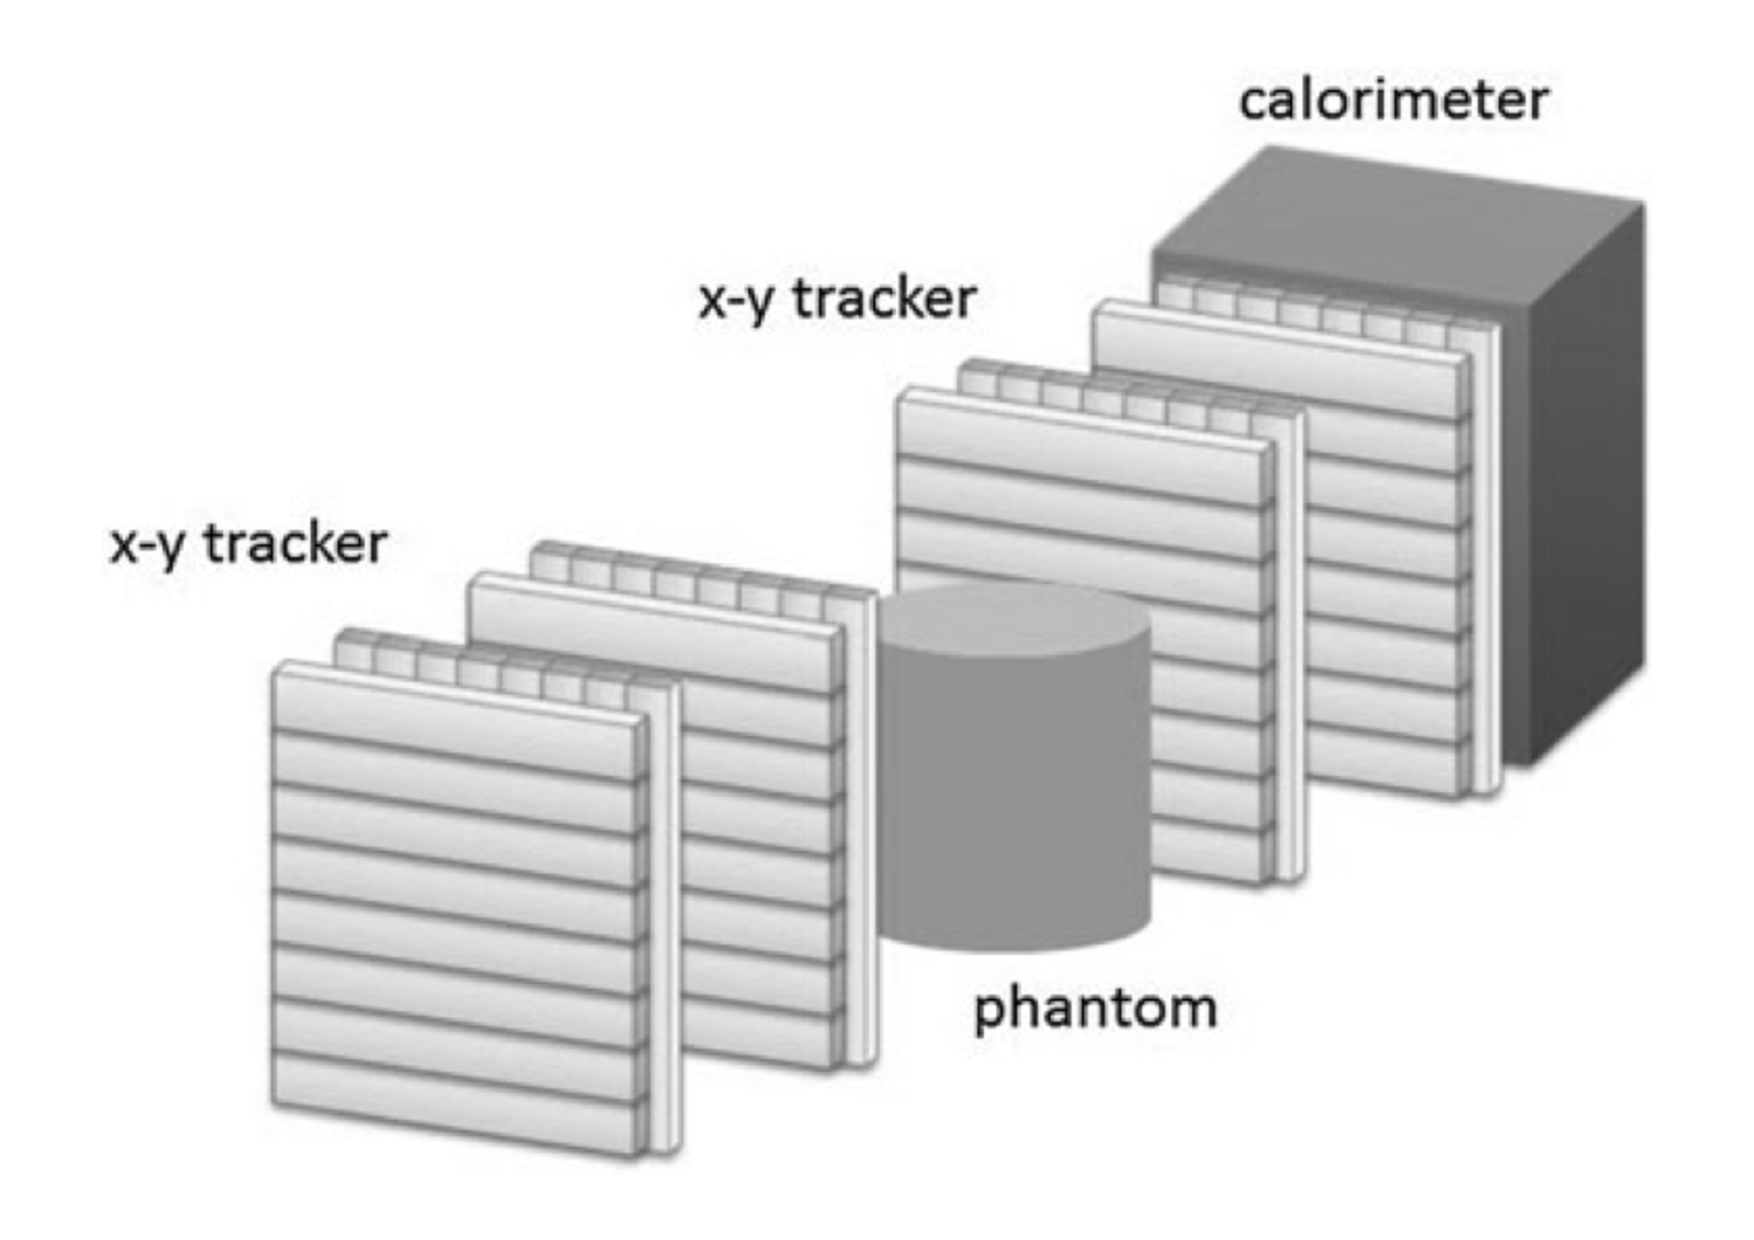
\includegraphics[width=0.9\linewidth]{03_GraphicFiles/chapter1_Introduction/pCT_general.pdf}
\caption{Schematic view of standard ion \gls{ct} detector design. Each primary incoming particle is tracked before the interaction in the patient and at the exit, and its residual energy is absorbed and measured by a calorimeter. In~\cite{Mattiazzo2015}.}
\label{chap1::fig::pCT_design}
\end{subfigure}
\begin{subfigure}[t]{.49\textwidth}
\centering
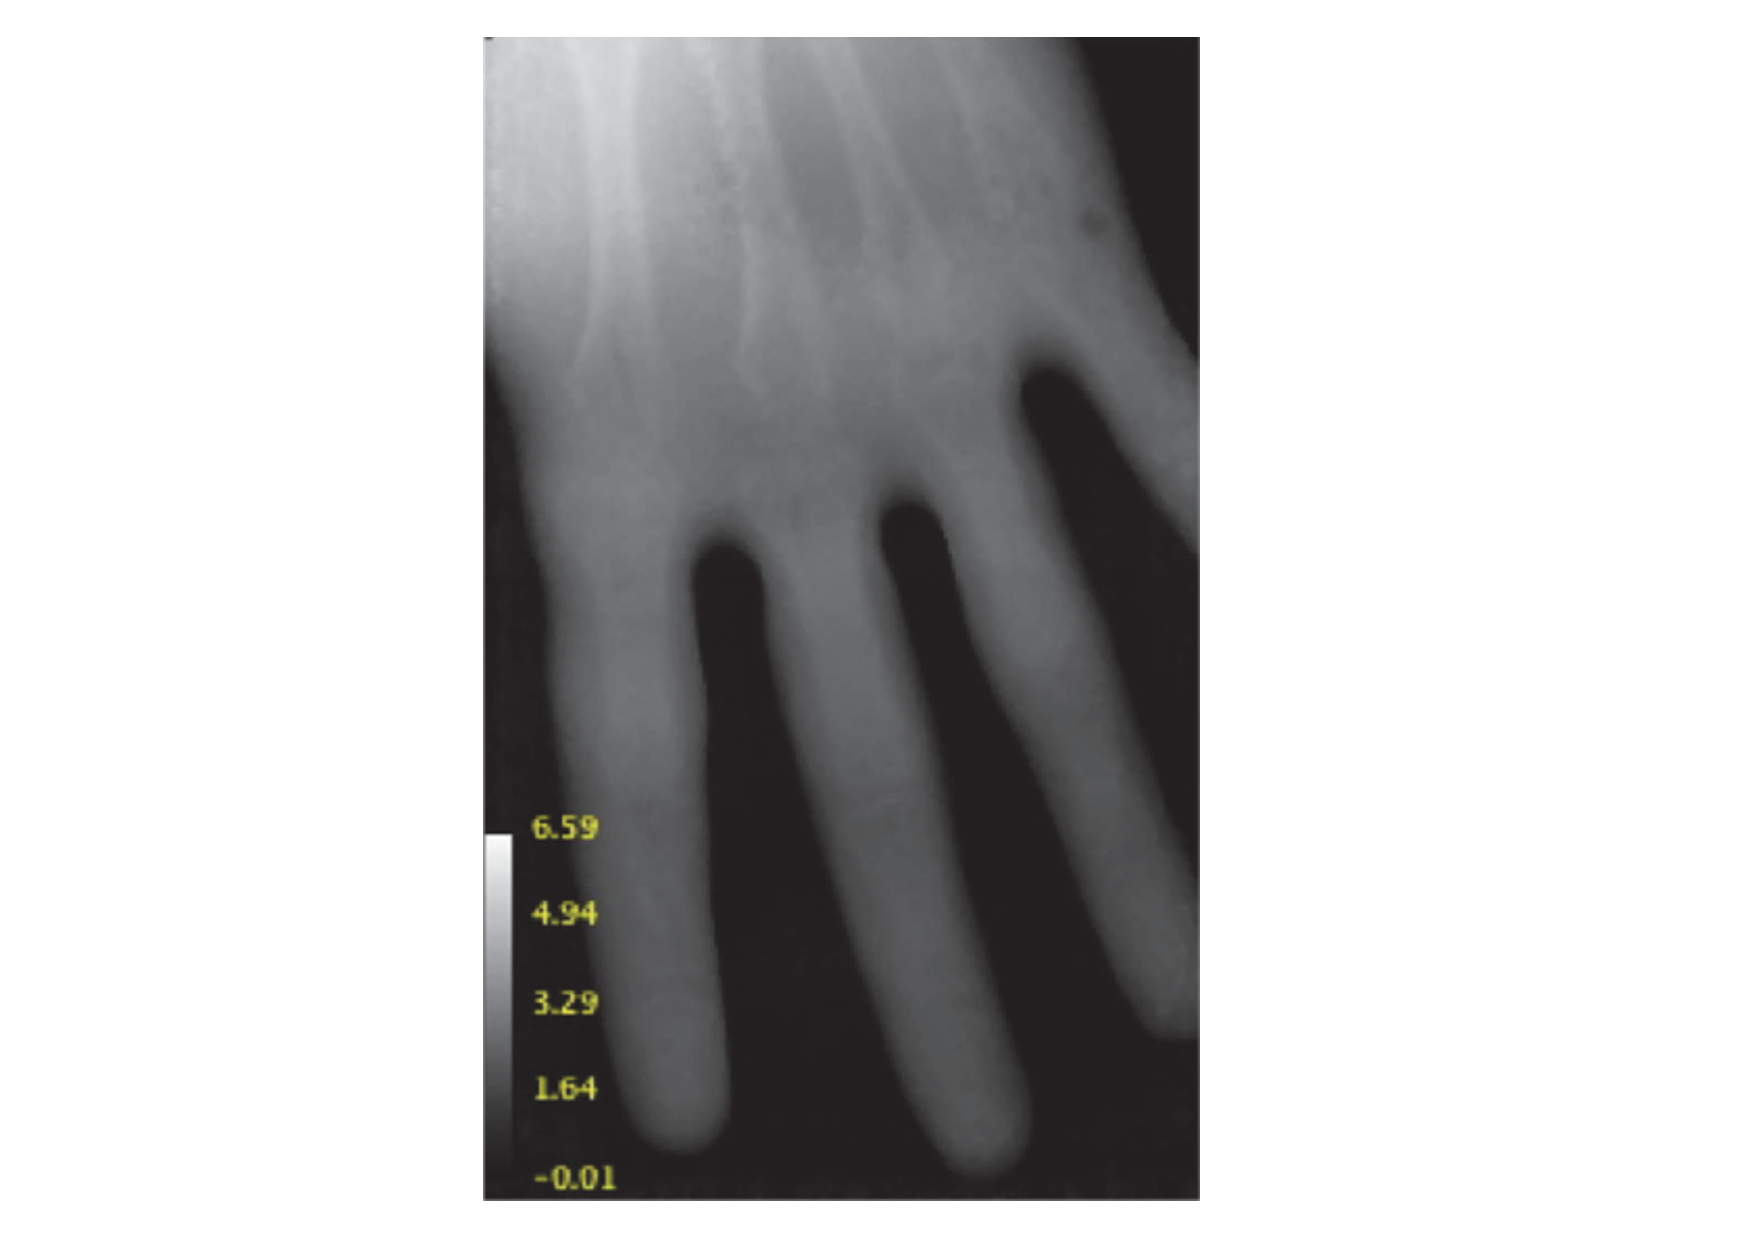
\includegraphics[width=0.92\linewidth]{03_GraphicFiles/chapter1_Introduction/pCT_image.pdf}
\caption{Proton \gls{ct} image of an hand phantom. In~\cite{Plautz2014}.}
\label{chap1::fig::pCT_image}
\end{subfigure}
\caption{Proton and heavier ion radiography and \gls{ct} are under study in the last years as promising techniques for optimizing the treatment planning performance in hadrontherapy. A standard detector design is sketched in the left panel, while the first image of an hand phantom is reported in the right one.}
\label{chap1::fig::ionCT}
\end{figure} 

Since all the primary incident particles must completely pass through the target for a residual energy measurements, the beam energy must be higher than the one applied for radiotherapy treatments. In the case of protons, standard clinical accelerators can provide beam at a maximum energy of 230-250~MeV (the projected range of 250~MeV protons in water is $\sim$38~cm - see \gls{nist} tables at~\cite{NISTpstar}), not enough to pass in all directions through the hip region of a typical adult, and far short of the shoulder-to-shoulder distance through a human male. Such energies are anyway sufficient for scanning the head or the lung region for most patients~\parencite{Johnson2017}. The optimal beam conditions for radiography have already been pointed out for protons in one of the first studies about this topic~\parencite{Moffett1975}. At that time, small pencil beams were preferred, with low intensity and limited energy spread. In reality, the beam can be also passively spread to cover the whole detector aperture, or a scanning technique can be used as suggested in the original papers. In addition to the first highlighted advantage of this technique, which provides direct access to stopping power data, there are other factors determining its convenience with respect to x-ray imaging. A dosimetric advantage with respect to x-rays has been already proven in 1975~\parencite{Moffett1975}, and a reduction of imaging dose by a factor 10 to 20 has been reported in ~\cite{Schneider1995}. Recent results showed, for equal spatial and density resolution, 50-100 times lower image exposure for protons with respect to x-rays~\parencite{Schneider2004}. Moreover, the low dose enables one to perform proton imaging scans before each treatment fraction: this is potentially very useful for positioning optimization (the scan is performed under the same geometrical conditions as the treatment) and for the detection of anatomical changes, which cannot be included in the present treatment planning, based on a single \gls{ct} scan performed before the beginning of the whole treatment cycle. However, it must be considered that ion radiographies are performed in the same treatment room and couch, limiting the patient flow. Moreover, a major limitation of proton radiography techniques is represented by a poor spatial resolution due to \gls{mcs}, already highlighted in the first publications~\parencite{Koehler1968, Moffett1975}. Several small angle deflections produce uncertainties in the reconstructed trajectories~\parencite{Schneider1995, Schneider2004, Penfold2009}. Heavier ions are less affected by \gls{mcs} in the target, so that better spatial resolution with respect to protons can be achieved, but they suffer from substantial nuclear spallation and the projectile and target fragmentation can add background to the final image~\parencite{Parodi2014}. The helium ions, which already have the advantage of requiring much less energy than carbon ions in order to fully penetrate a phantom, behave more like protons within the phantom, but with significantly reduced scattering and increased spatial resolution. Helium, indeed, appears to be the optimum compromise, even if it is not implemented in clinics for tumor treatments at present. With the increasing diffusion of heavy-ion therapy centers, anyway, we can expect a further development of this field in the next years~\parencite{Parodi2014}.
The described ion transmission imaging method provides two-dimensional information, but it can be extended into 3D with the rotation of the system around the target (or the patient rotation) and the application of tomographic reconstruction. The so-called ion-\gls{ct} makes use of optimized \gls{fbp} methods or \glspl{art} to obtain 3D patient images by combining various data sets from different angles.
At present, ion transmission imaging for both radiography and tomography is not yet clinically implemented, but a number of research groups conducts instrumental development campaigns to produce prototypes to be tested in clinics. Although the basic design is common, with tracker and absorber components, different technological solutions are being explored. The first prototype designed for this purpose, after the first trial conducted at the early stage of this research field, was studied at \gls{psi}; it was based on a pair of \glspl{mwpc} as tracker, followed by a \gls{nai} 7.5~mm diameter crystal for the energy measurement~\parencite{Schneider1995}. The detector was later upgraded to overcome rate and size limitations, with the use of scintillating fiber hodoscopes instead of \glspl{mwpc} and plastic scintillator tiles to substitute the monoblock \gls{nai} crystal~\parencite{Pemler1999}. Similar scintillating-fiber trackers have been used by the OFFSET collaboration for its prototype~\parencite{Lopresti2014}, which showed very low efficiency. The same author recently presented a beam monitoring and radiography prototype (QBeRT) with upgraded read-out system, providing enhanced results~\parencite{Lopresti2016, Gallo2016}. The TERA Foundation at CERN has been involved for several years in the development of detectors to be applied in the quality assurance for hadrontherapy. Within the Advanced QUality Assurance (AQUA) project~\parencite{Amaldi2010b}, proton radiography instruments were developed and tested on clinical beams, starting from 2009. The first prototype, based on \gls{gem} detectors~\parencite{Sauli1997} for tracking and plastic scintillator layers for the calorimeter, had an active area of 10$\times$10~cm$^2$~\parencite{Amaldi2011}, then extended to 30$\times$30~cm$^2$ for the second version of the machine, with similar detection technologies but improved rate acceptance capabilities thanks to new read-out systems~\parencite{Bucciantonio2013, BucciantonioPhD2015}. A complete, wide surface proton \gls{ct} system has been proposed by an American collaboration of the \gls{niu}and the \gls{fnal}~\parencite{Naimuddin2016}. It is based on 0.5~mm diameter scintillating fibers read out by SiPM, for an active area of 24$\times$20~cm$^2$. Alternative, more expensive designs include silicon-strip detectors for proton tracking, such as the one in development in Italy by the PRIMA collaboration, with eight layers of silicon sensors and a calorimeter composed of a 2$\times$7 array of \gls{yagce} crystals, 3$\times$3~cm$^2$ section and 10~cm length each~\parencite{Scaringella2013}. The experience of a collaboration of the \gls{llu} and the \gls{ucsc} started with a small prototype with slow acquisition~\parencite{Sadrozinsky2011}, based on doped \gls{csi} crystal to measure the residual range, then extended to a larger one~\parencite{Johnson2016}, sufficient for a human head scan, which already provided advanced results. The \enquote{Phase-II Scanner} is based on two silicon-strip detector modules for the tracking section and five polystyrene-based scintillator segments for the range measurements. In \figurename~\ref{chap1::fig::pCT_image} a proton \gls{ct} image of an head phantom obtained with the first generation detector is shown. A similar system has also been studied in simulation by a group in Korea~\parencite{Lee2016}. The same tracking detectors are used in a Japanese collaboration project; the group developed a slow-acquisition and small aperture prototype and already planned an upgrade to a ten times larger system with increased acquisition rate capabilities~\parencite{Saraya2014}. The British collaboration \gls{pravda} tested a first prototype of a proton \gls{ct} system entirely based on silicon detectors~\parencite{Taylor2014, Taylor2016}. An alternative and simpler approach has been investigated with a system using a stack of 40 nuclear emulsion plates which records the proton tracks then reconstructed off-beam~\parencite{Braccini2010b}; the results are interesting, even if such a solution is not suitable for real-time imaging.   
Even if the majority of the research efforts are devoted to proton application of the radiography/tomography technique, some tests has been made also for heavier ions. At \gls{nirs}, a combination a fluorescent screen viewed by a \gls{ccd} camera and rotational range shifters has been investigated~\parencite{Abe2002}, together with a more conventional system composed of scintillating fibers for tracking and a thick plastic absorber~\parencite{Shinoda2006}. At \gls{hit}, studied setups involved silicon flat panel detector~\parencite{Telsemeyer2012} or a range telescope consisting of a stack of parallel plate \glspl{ic} with 3~mm thick plastic absorbers~\parencite{Rinaldi2013}. All the listed systems produced promising results~\parencite{Parodi2014}.
    
\subsubsection{Positron Emission Tomography}\label{chap1::subsubsec::RangePET}
As explained in section~\ref{chap1::subsubsec::ionInteractions}, the fragmentation processes involving target nuclei during proton therapy irradiation and both projectile and target nuclei in case of heavier ion beam therapy, can produce radioactive isotopes. In particular, $\beta^+$ emitting fragments are of significant interest for range verification purpose. Table~\ref{chap1::tab::petIsotopes} shows the main reaction channels and relative isotopes produced along a proton beam path in tissue. More details about the most relevant reaction channels and their characteristics (energy threshold, isotope decay constant, maximal kinetic energy of the emitted positrons), can be found in~\cite{Oelfke1996}. Additional channels and isotopes are produced during carbon ion irradiation, given the possible projectile activation. 

\begin{table}[!htbp]
\centering
\caption{Proton-nuclear reaction channels and relative positron emitters produced in human tissues. Table reproduced from~\cite{Espana2011b}.}
\label{chap1::tab::petIsotopes}
\resizebox{\textwidth}{!}{%
\begin{tabular}{llcc}
\toprule
\rowcolor{myColorMainA!20} 
\textbf{Target}& \textbf{Nuclear reaction channel} & \textbf{$\beta^+$ isotopes} & \textbf{Half-life} \\
\midrule
C & $^{12}$C(p, pn)$^{11}$C, $^{12}$C(p, p2n)$^{10}$C & $^{10}$C, $^{11}$C & 19.29~s, 20.33~min\\
N & $^{14}$N(p, 2p2n)$^{11}$C, $^{14}$N(p, pn)$^{13}$N, $^{14}$N(p,n)$^{14}$O & $^{13}$N ($^{11}$C, $^{14}$O) & 9.96~min \\
O & $^{16}$O(p, pn)$^{15}$O, $^{16}$O(p, 3p3n)$^{11}$C, $^{16}$O(p,2p2n)$^{13}$N, $^{16}$O(p,p2n)$^{14}$O, $^{16}$O(p,3p4n)$^{10}$C   &  $^{14}$O, $^{15}$O, ($^{11}$C, $^{13}$N)& 70.61~s, 122.24~s\\
P & $^{31}$P(p, pn)$^{30}$P&$^{30}$P & 2.50~min\\
Ca & $^{40}$Ca(p, 2pn)$^{38}$K & $^{38}$K & 7.64~min\\
\bottomrule
\end{tabular}}
\end{table}    

\begin{figure}[!htbp]
\centering
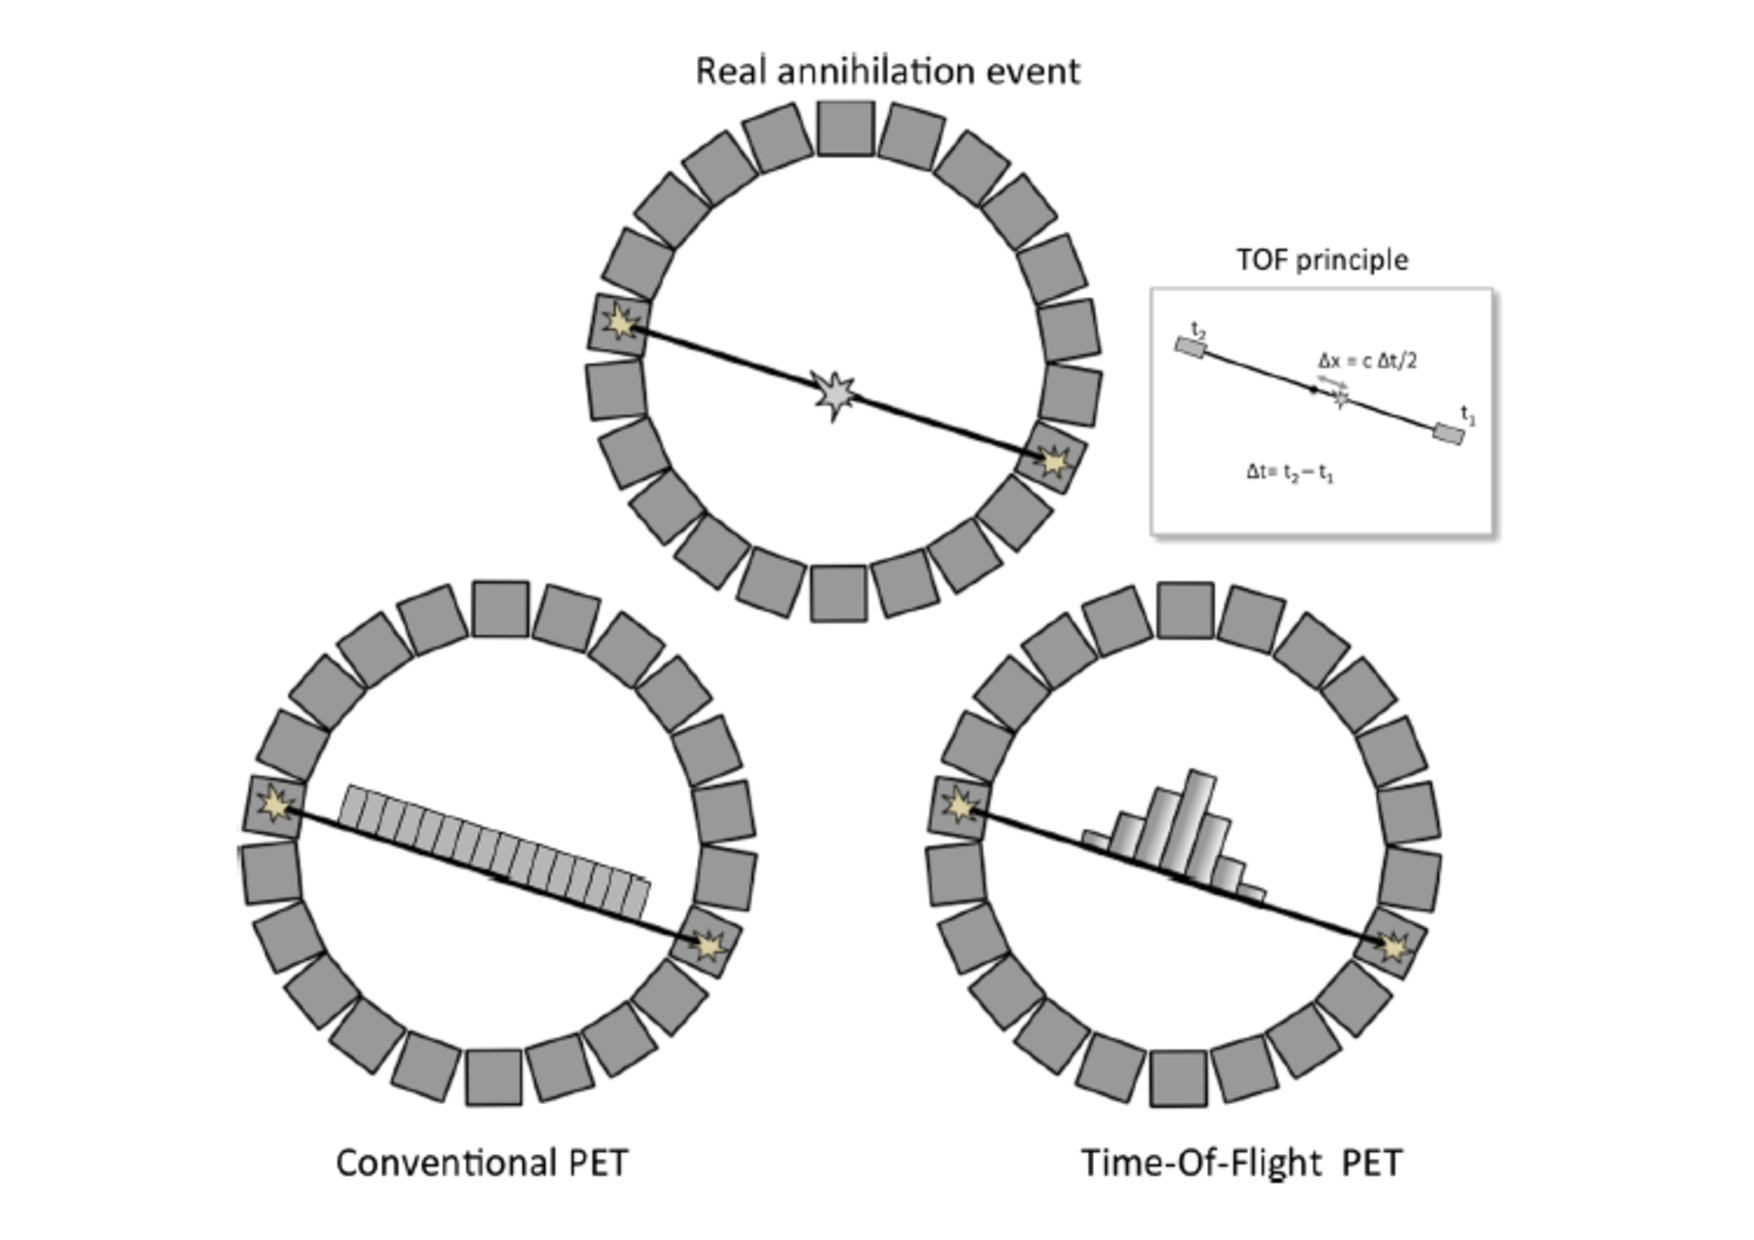
\includegraphics[width=0.8\textwidth]{03_GraphicFiles/chapter1_Introduction/PET_concept.pdf}
\caption{Schematic representation of the \gls{pet} technique principle. In the top figure, a standard real annihilation event is presented, while in the bottom line the principle of conventional and \gls{tof}-\gls{pet} are compared. In~\cite{Vandenberghe2016}.}
\label{chap1::fig::PETconcept}
\end{figure}   

\figurename~\ref{chap1::fig::PETconcept} (top) shows the concept of the \gls{pet} detection technque. The emitted positrons annihilate with human tissue electrons after traveling few mm distances, and 511~keV back-to-back photons are produced and can be detected in coincidence with \gls{pet} machines. The spatial distribution of the $\beta^+$ decay points can be then obtained via the reconstruction of the so-called \enquote{lines of response} connecting the two detected photons, and it correlates, even if not directly, to the dose profile. \figurename~\ref{chap1::fig::PETrangeProf} shows the one-dimensional $\beta^+$ activity profiles along the beam axis for various incident beam types impinging on a \gls{pmma} target. The positron emitter distribution dependence on the beam nature clearly emerges from these profiles, but a form of indirect correlation with the dose profile distal edge is always verified. In particular, a remarkable difference exists between light ions (protons, $^3$He and $^7$Li), for which the induced activity is almost only due to target residuals, and heavier ones ($^{12}$C and $^{16}$O), with a considerable contribution also coming from projectile fragmentation sub-products, which concentrate near the end of the range, explaining the activity peak. The investigation of the correlation between delivered dose and $\beta^+$ detected activity must face several issues, as highlighted in~\cite{Parodi2004}, mainly connected to the difficulty to retrieve quantitative information from \gls{pet} images and to wash-out effects. Long-lived positron emitters, indeed, can be transported away from the production point by blood flow and metabolic processes, affecting the precision of the obtained images. This effect has been deeply studied experimentally at \gls{himac} with rabbit tissues and Anger-type scintillation cameras~\parencite{Mizuno2003, Tomitani2003}, and, more recently, at \gls{gsi} with $^{12}$C beams~\parencite{Fiedler2008}. A reduction of a factor up to 1.5 in the precision of the range determination due to wash-out processes is reported, and a correlation between biological half-life and local dose has been verified and used in simulation to improve the quality of \gls{pet} images. Although several research efforts have been dedicated to improve the precision of the dose recovery from $\beta^+$-emitter distributions~\parencite{Parodi2006, Parodi2007, Parodi2010}, the only feasible solution for the monitoring of dose delivery is the comparison of measured distributions to simulated ones~\parencite{Ponish2004}. These Monte Carlo simulations are based on the planning \gls{ct} scan, the irradiation scheme, the detector geometry, the imaging procedure; deviations in the delivered dose caused by patient positioning or anatomical modifications can be detected, mainly because they are reflected in changes in the maximum particle range in the target tissues. Thus, the main quality criterion of the \gls{pet} monitoring method is the precision in the measurement of range shifts with respect to the predicted ones~\parencite{Fiedler2010}. The accuracy of the reference simulated activity distribution has advanced in the last years, but it is still limited by the lack of underlying cross-sectional data, the not perfect knowledge of the elemental composition of the patient and the complex prediction of metabolic wash-out processes. Complementary imaging modalities can give fundamental contributions to the simulation predictions: for example, the use of supplemental \gls{mri} data has been proposed to better analyze local wash-out effects. In addition to this, the implementation of hybrid \gls{pet}-\gls{ct} systems, preferably with dual-energy \gls{ct}, would improve the conversion of \gls{ct} information to the material composition needed for the \gls{pet} simulations~\parencite{Landry2013}.  

\begin{figure}[!htbp]
\centering
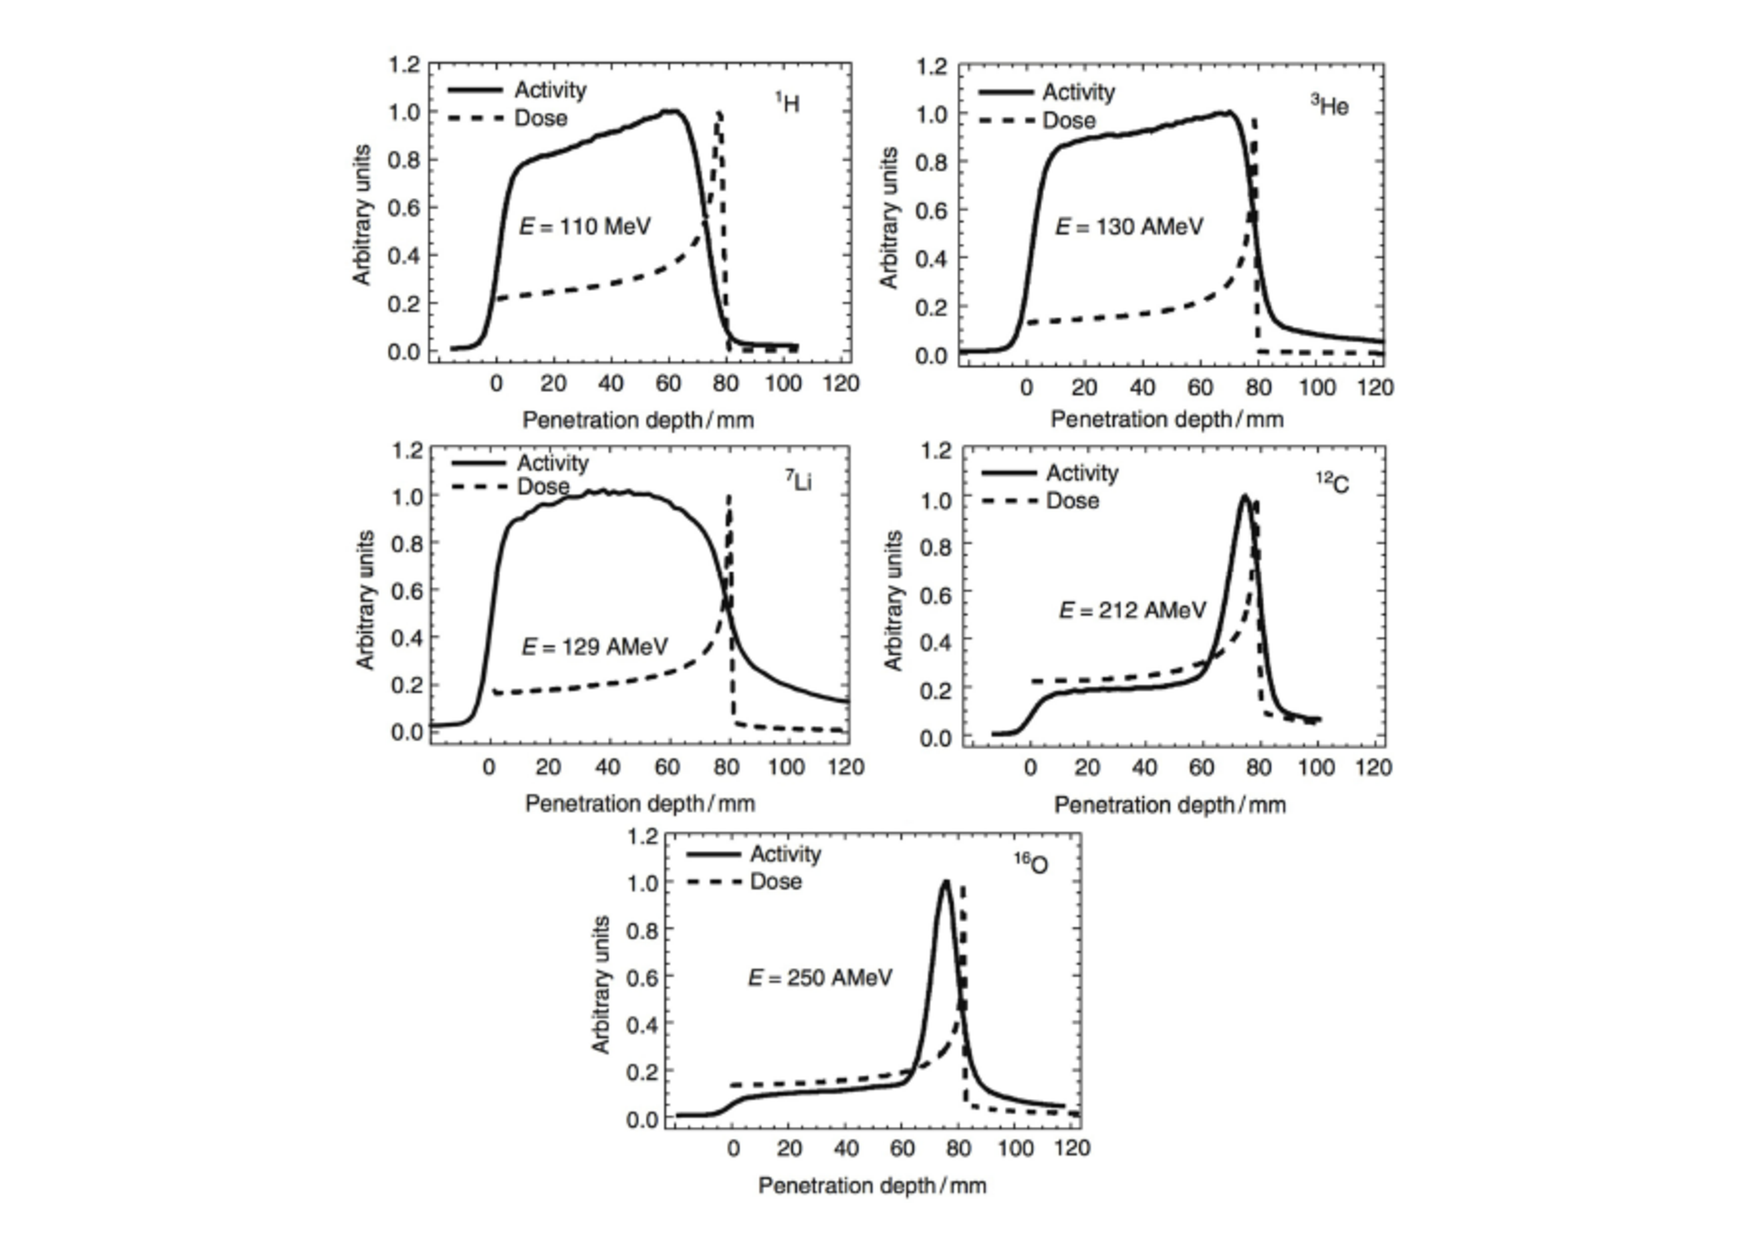
\includegraphics[width=0.98\textwidth]{03_GraphicFiles/chapter1_Introduction/PETrangeProf.pdf}
\caption{$\beta^+$ activity profiles for various ion beams impinging on a \gls{pmma} thick target. The depth-dose profiles are also shown in dashed lines for comparison. In~\cite{Fiedler2012}.}
\label{chap1::fig::PETrangeProf}
\end{figure}   

The \gls{pet} data acquisition can be performed following three main strategies:
\begin{itemize}
\item In-beam data acquisition: the \gls{pet} system is integrated in the beam delivery system and the data acquisition is performed during or immediately after irradiation in the treatment room. In synchrotron facilities, a further solution is represented by acquisitions in the time between different spills, while for cyclotrons data-taking during beam extraction has been explored and seems feasible~\parencite{Kraan2014}. On one hand, this method is advantageous because it allows detecting short-lived isotopes, thus increasing the available statistics, and reducing the effects of biological processes. Moreover, the patient position does not change with respect to the treatment. On the other hand, the integration of \gls{pet} scanners in the treatment site can be costly and cause limitations on the detector geometry affecting detection efficiency and, consequently, image quality. The scanner should not be directly exposed to the beam in order to avoid damage and activation of active modules and electronics, and at the same time it should allow enough degrees of freedom for the patient table. The need of an opening for the beam portal typically results in the choice of planar dual-head configurations.
\item In-room data acquisition: the installation of commercial full-ring \gls{pet} scanners in the treatment room, but not directly on the beam line, allows the so-called \enquote{in-room} data acquisitions quickly after the end of the treatment irradiation. This solution leads to longer treatment room occupation, because some minutes of imaging time is required to gain enough statistics, but allows one to use commercial machines, less expensive and more efficient than custom integrated scanners designed for in-beam applications. Moreover, patient positioning issues are minimized by the limited movements and signal wash-out is reduced.
\item Off-line data acquisition: if the patient has to be transported out of the treatment room for the \gls{pet} scan, the implemented strategy is classified as \enquote{off-line}. The limited cost and treatment occupation time are probably the only advantages of this method, which suffers from relevant signal decay and wash-out processes given the long time between the end of the irradiation and the beginning of the \gls{pet} scan. Off-line images predominantly show activity from isotopes whose half-life is comparable or longer then the transportation and setup time, thus it is mainly restricted to $^{11}$C (half-life longer than 20 minutes), produced in relative small amount in proton therapy, more abundant in carbon treatments. The reduced number of available decays requires longer acquisition time with respect to in-beam and in-room solutions, which further enhance the effect of metabolic processes. The patient repositioning issues also contribute to the image quality degradation. 
\end{itemize}
A schematic view of the three \gls{pet} acquisition modalities is presented in \figurename~\ref{chap1::fig::PETmodes}. As mentioned in the three data acquisition modality description, the counting statistics is one of the fundamental parameters to be studied for the design of \gls{pet} monitoring solutions. It can be estimated as the integral of the decay curve shown in \figurename~\ref{chap1::fig::PETactDistr}, where the time intervals corresponding to the three acquisition strategies are separated. The curve is based on measurements performed at \gls{gsi} during therapeutic irradiation with carbon ions; an in-beam solution has been adopted, with 40~s additional data taking time after the irradiation. The in-room selected window lasts 3 minutes, and for the off-line case, long-time measurements of one patient have been used~\parencite{Fiedler2008b}. If 100\% is assigned to the number of registered true events in the in-beam condition, 50\% is estimated for the in-room solution and 58\% for the off-line data taking~\parencite{Shakirin2011}. It is then clear that off-line solutions are severely challenged by the extremely low signal, considerably lower with respect to the standard application of the employed commercial scanners (down to average activity values of few tens of Bq/ml~\parencite{Bauer2013}).
The scanner geometry is another fundamental parameter to be considered: as mentioned, the chosen data-acquisition strategy determines the scanner design. In-room and off-line solutions can make use of commercial full-ring systems, with a complete field of view. In addition to this, modern combined \gls{pet}-\gls{ct} scanners enable an accurate co-registration of treatment and imaging position, so that the unavoidable patient movement due to transportation and repositioning can be partially corrected. The geometrical constraints imposed by in-beam integrated solutions cause reduced efficiency and restricted field-of-view, which are reflected in image artifacts~\parencite{Crespo2006}, particularly significant in the imaging of large tumor objects. Improvement can be provided by \gls{tof}-\gls{pet} detectors~\parencite{Crespo2007, Surti2011}, as discussed below.
In~\cite{Parodi2015} the author highlights how the first historical attempts to implement \gls{pet} particle therapy monitoring, described in the following, have not relied on optimized instrumentation for the peculiar application. Anyway, the promising results obtained by several groups encouraged dedicated investigations which are leading to substantial improvements of such a technique in the last years. In particular, the application of gamma detectors with depth-of-interaction capability, also studied for standard diagnostics applications, has demonstrated its effectiveness in correcting parallax artifacts in the reconstructed images; improvements in data acquisition and synchronization with the accelerator radio-frequency offer the possibility of including the signal detected during the beam-on time for in-beam solutions, thus increasing the counting statistics and reducing the acquisition time; new adapted geometries, such as the Japanese OpenPET system~\parencite{Tashima2012, Yamaya2008}, recently finalized in its upgraded version~\parencite{Yamaya2017}, offer higher-efficiency alternatives to standard dual-head systems. 
It is worth to dedicate particular attention to the already mentioned \gls{tof}-\gls{pet}, deeply studied in the last years, which already demonstrated improved imaging capabilities with respect to standard scanners. The measurement of the detection time of each of the two photons helps, through the calculation of the arrival time difference, in restricting the emission point along the reconstructed line of response and thus also in rejecting part of accidentals. In standard \gls{pet}, the three-dimensional reconstruction relies on the superposition of several lines of response and on filtered back-projection algorithms. The time information adds a second dimension to the line of response reconstruction, with the localization of the interaction point in a few cm along the line, depending on the detector time resolution. For example, a coincidence timing resolution of 600 ps \gls{fwhm} translates to a position uncertainty of 9 cm \gls{fwhm}. In~\figurename~\ref{chap1::fig::PETconcept} (bottom line), the \gls{tof}-\gls{pet} principle is sketched and compared to the conventional \gls{pet} detection scheme. 
The potential benefits of \gls{tof} information in \gls{pet} image reconstruction were already understood since the early stage of its development for diagnosis purpose, and the first \gls{tof}-\gls{pet} systems were built already in the 1980s in the US~\parencite{Gariod1982}. They were based on \gls{csf} or \gls{baf2} scintillators, the best available at the time in terms of time resolution, but their spatial performance and sensitivity were poor with respect to conventional \gls{pet} scanners. The improvements in scintillating material as well as in \gls{pm} performance and reliability allowed for the first commercial proposal of a \gls{tof}-\gls{pet} scanner only in 2006, by Philips~\parencite{Surti2007}. The development of \gls{tof}-\gls{pet} machines is strongly connected to their application in diagnosis, and further details will be given in section~\ref{chap1::subsec::PET_NM}. As for particle therapy monitoring application, the \gls{tof} technique applied to \gls{pet} can be used to partially reverse the effects caused by non-complete angles of in-beam data collection~\parencite{Crespo2006}, and in general to improve the image quality. Various groups are developing detector solutions for clinical implementation of such a technique; some of them have already been tested on beam with promising results. They will be described in more details in the following, after a brief historical overview of the \gls{pet} application in particle therapy quality assurance. 

\begin{figure}[!htbp]
\begin{subfigure}[t]{.49\textwidth}
\centering
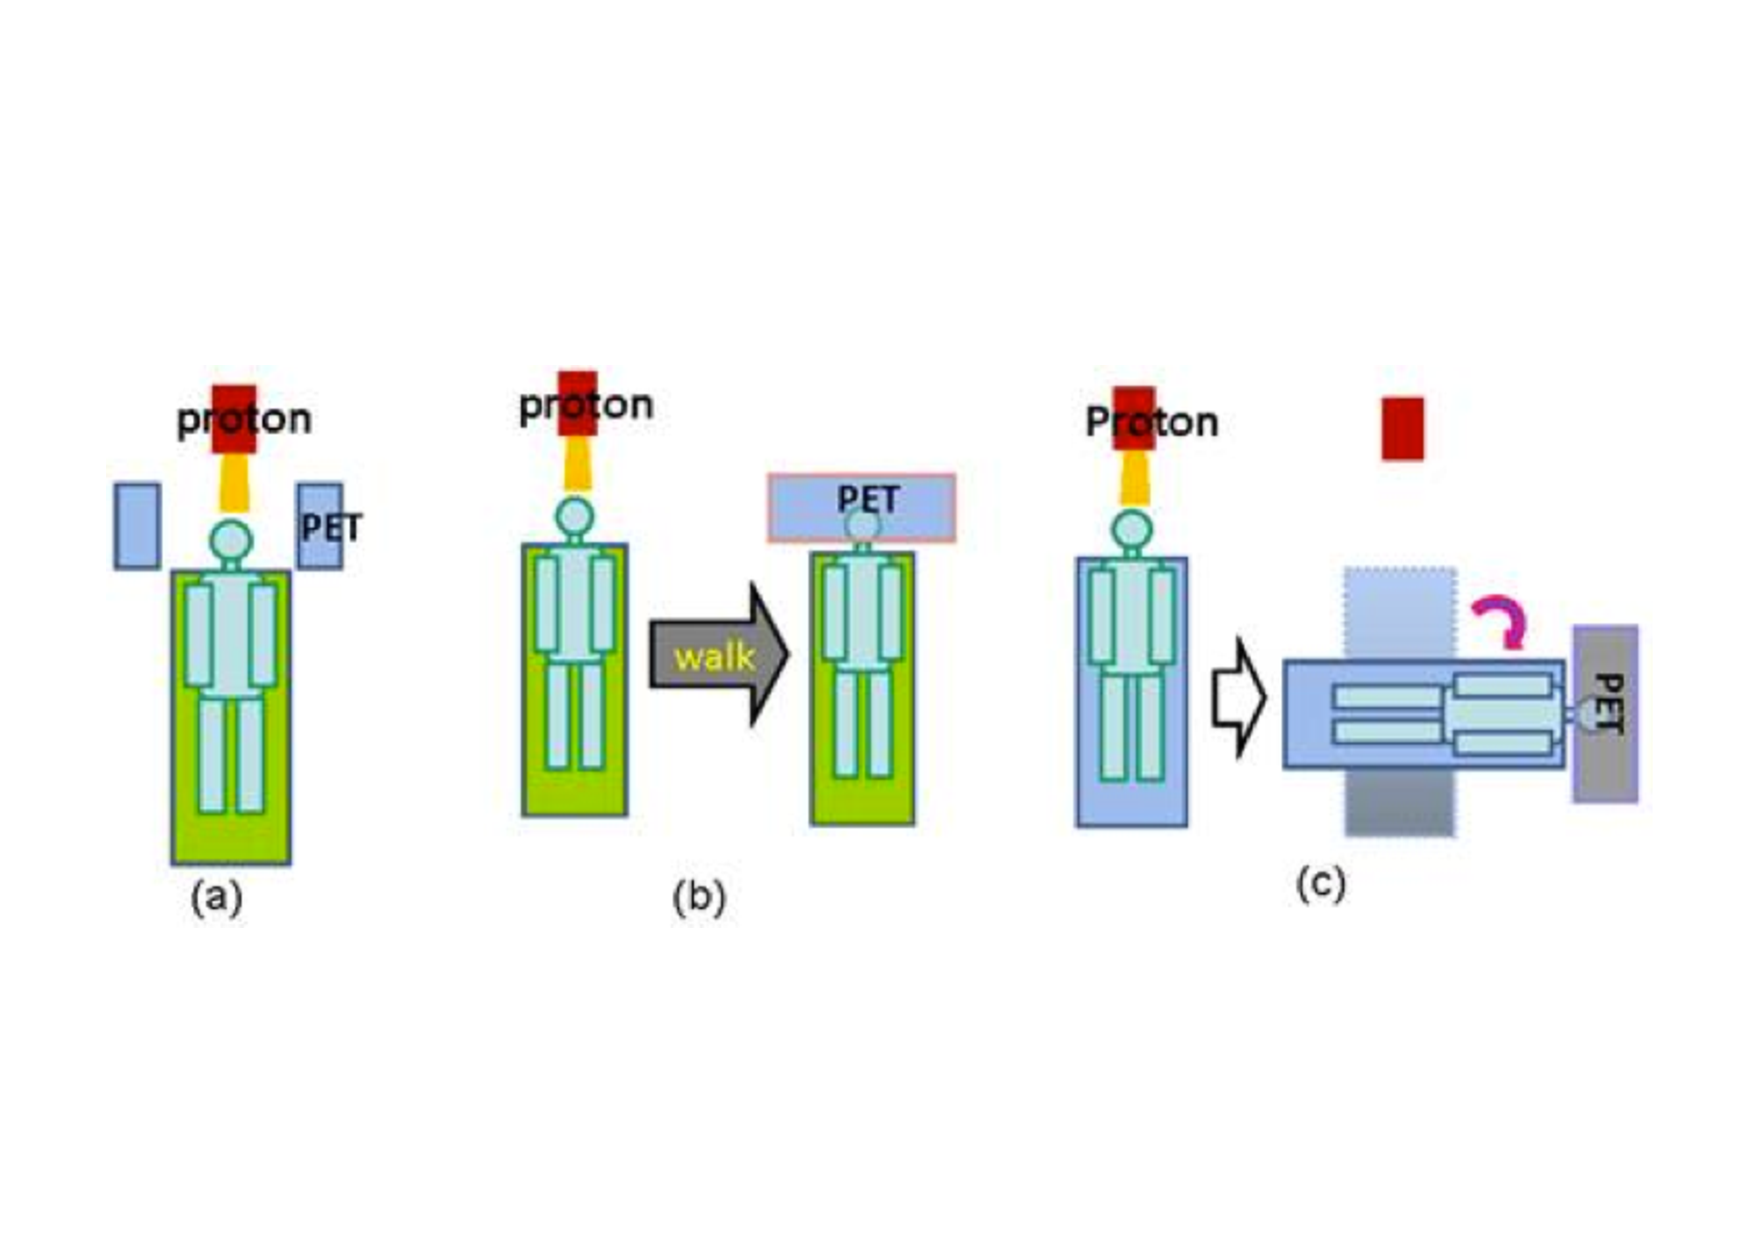
\includegraphics[width=0.98\linewidth]{03_GraphicFiles/chapter1_Introduction/PETmodes.pdf}
\caption{Schematic view of the three \gls{pet} configurations for the application in ion range monitoring. Form left to right: in-beam, off-line and in-room \gls{pet}. In~\cite{Zhu2013}.}
\label{chap1::fig::PETmodes}
\end{subfigure}
\begin{subfigure}[t]{.49\textwidth}
\centering
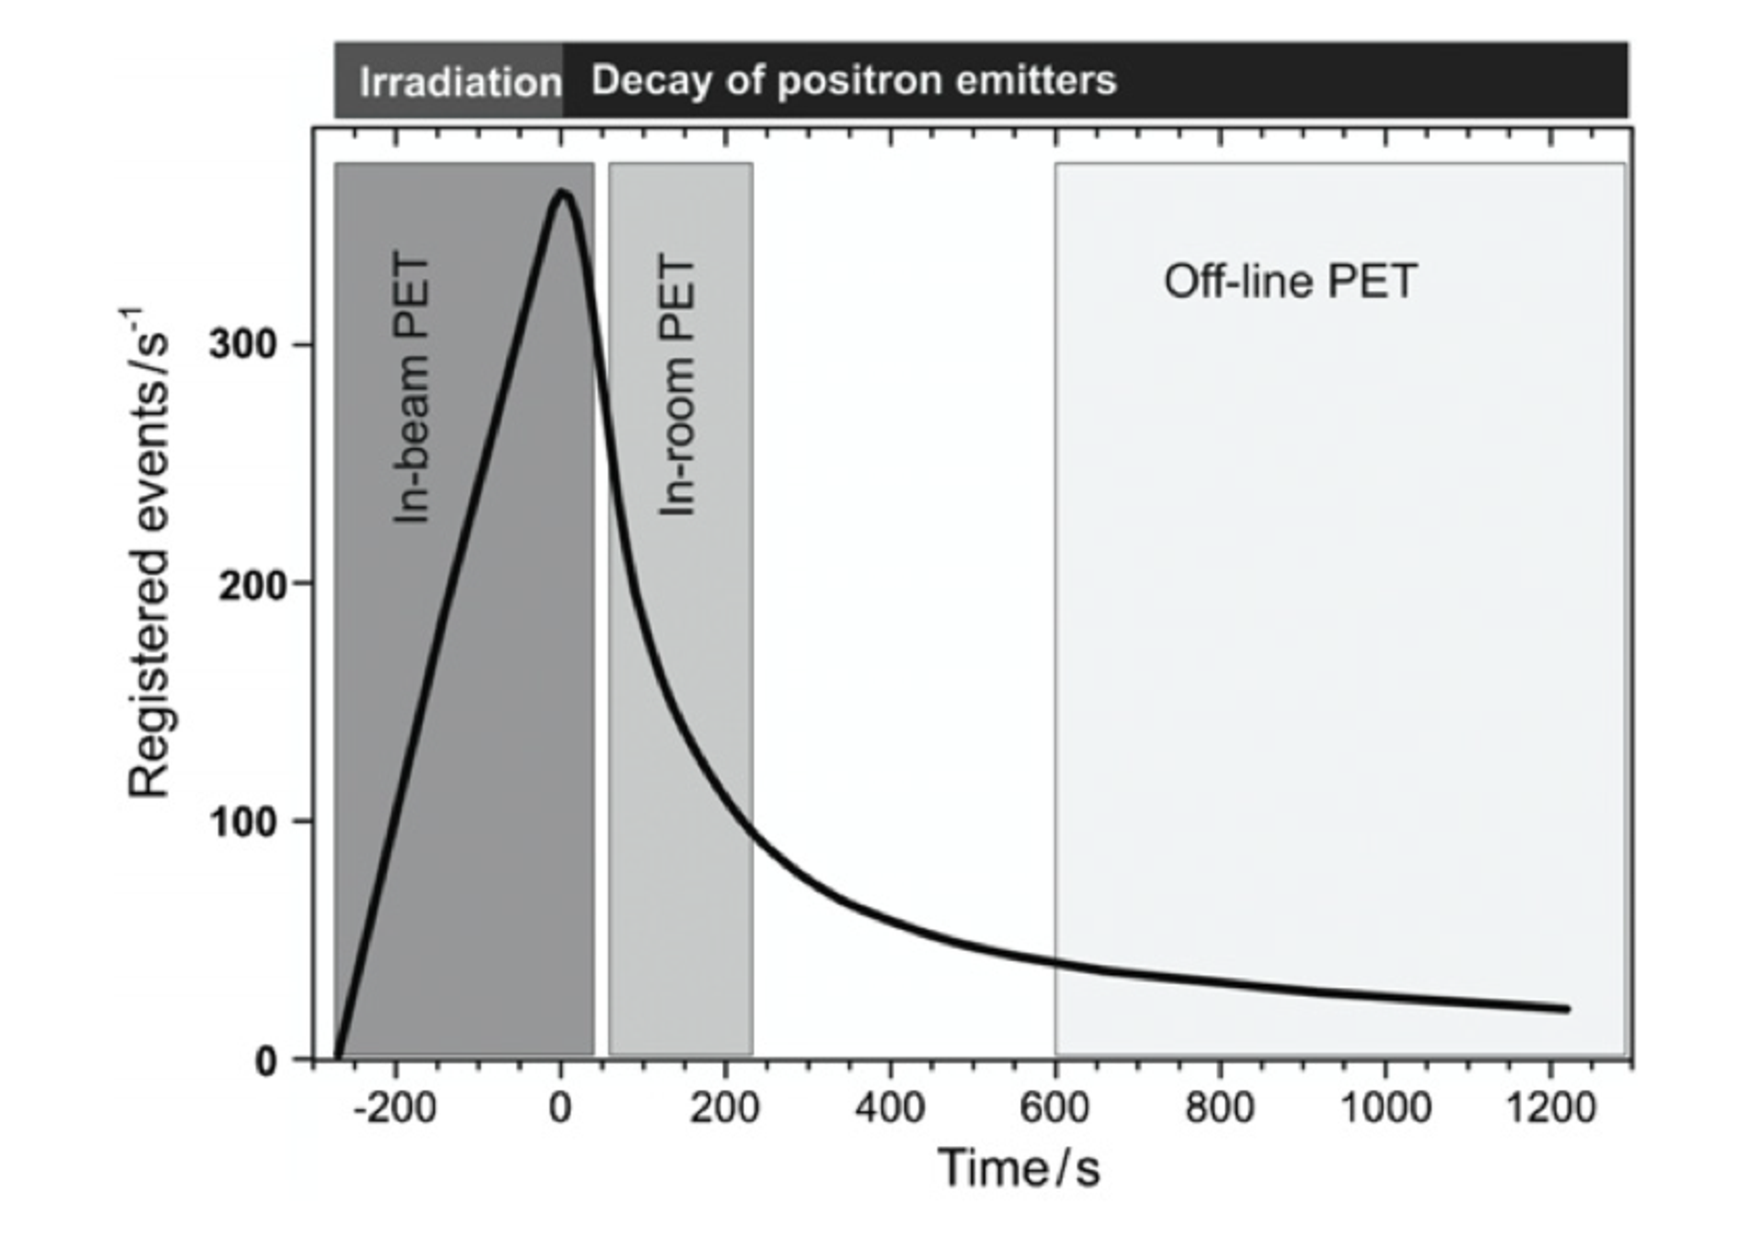
\includegraphics[width=0.92\linewidth]{03_GraphicFiles/chapter1_Introduction/PETactDistr.pdf}
\caption{\gls{pet} registered events as a function of time corresponding to the measurement of one field during
irradiation and up to 20 minutes after irradiation. The time intervals corresponding to  in-beam, in-room, and off-line \gls{pet} measurements are highlighted. In~\cite{Shakirin2011}.}
\label{chap1::fig::PETactDistr}
\end{subfigure}
\caption{The application of the \gls{pet} technique to the monitoring of ion range in particle therapy includes three possible modalities: in-beam, in-room and off-line \gls{pet}, represented in the scheme in (a). The amount of registered events depends on the created positron emitter half-life, and thus on the implemented modality, as shown by the histogram in (b).}
\label{chap1::fig::PETmodalities}
\end{figure} 

As emerges from the above paragraphs, \gls{pet} is probably the most extensively studied technique for online beam range verification and is at present the only method clinically implemented~\parencite{Enghardt2004}. The first published proposal of using \gls{pet} for range verification in particle therapy dates back to 1975~\parencite{Bennett1975}. In the next years, further suggestions were connected to pion~\parencite{Goodman1986, Shirato1989} and neutron therapy~\parencite{Vynckier1989}, but the actual clinical implementation was pioneered in the context of heavy ion therapy at \gls{lbl}~\parencite{Llacer1979, Chatterjee1981}. The original idea was to verify the correctness of $^{20}$Ne ion therapy treatment plans by delivering a low dose $\beta^+$ emitting ion beam (e.g. $^{19}$Ne) prior to the treatment and measuring its range via \gls{pet} imaging of the emitted photons; before the regular treatment with stable beams. Pilot experiments were conducted with a planar \gls{pet} camera based on two blocks of \gls{bgo} crystals, including measurements in a live dog~\parencite{Llacer1984b}. The experimental data showed interesting results, even if the use of a passive beam shaping system determined a significant activation of the \gls{bgo} camera (mainly due to neutrons) and, thus, a substantial noise level. Analog investigations using radioactive ion beams ($^{15}$O, $^{17}$F, $^{19}$Ne) were carried out in the nineties at \gls{gsi} with various \gls{pet} cameras~\parencite{Pawelke1996}, and further developments of this technique were obtained at the \gls{himac} facility~\parencite{Iseki2004, Kitagawa2006}, where a dedicated line was set up for radioactive beam based treatments~\parencite{Urakabe2001, Kanazawa2002}. The \enquote{autoactivation} process~\parencite{Tobias1971} described above (i.e. the production of radioactive nuclei in the target by incident beam of stable ions) makes anyway possible the implementation of \gls{pet} monitoring techniques on standard high-energy beams, and the first clinical implementation of such  technique was launched at \gls{gsi} in 1997, after the tests with radioactive beams mentioned above and fragmentation studies conducted with $^{12}$C, $^{16}$O, $^{20}$Ne beams on a \gls{pmma} target~\parencite{Enghardt1992}. An in-beam \gls{pet} system was designed and installed into the treatment room and has been employed routinely for monitoring the irradiation of more than 440 patients (mainly suffering from head-and-neck cancer), with data acquisitions performed in the pause of pulsed beam delivery. This experience proved how \gls{pet} is a valuable tool for particle therapy quality assurance~\parencite{Enghardt2004}. In parallel to these developments in Germany, an off-line solution was implemented at \gls{nirs} with a commercial full-ring volumetric scanner, but it was not used in clinics. As previously explained, notwithstanding the lacking peak structure in the activity profile (cf. \figurename~\ref{chap1::fig::PETrangeProf}), also proton irradiation therapy can be monitored by \gls{pet} scanners. Various detailed studies investigated its feasibility and performance in the nineties~\parencite{Litzenberg1992, Paans1993, Oelfke1996, Litzenberg1999}. Two groups worked in parallel on clinical studies of \gls{pet} monitoring in proton therapy. In Japan, a dual-head \gls{pet} scanner has been installed at the National Cancer Center, Kashiwa~\parencite{Nishio2006}: it is based on high-resolution \gls{bgo} detector components and integrated in the proton gantry. The measurements are collected immediately after irradiation (in-room solution), mainly due to the considerable radiation background during the continuous beam delivery and the passive beam shaping. The satisfactory results led to the implementation of a daily \gls{pet} workflow, which allowed the research group to follow the anatomical changes of the patient during the treatment progress and correct the treatment planning. The test of this method included 48 patients suffering from head-and-neck, liver, lung, prostate and brain tumors~\parencite{Nishio2010}. In the US, at the \gls{mgh}, Boston, a pilot clinical study was performed with an off-line solution which made use of a commercial full-ring scanner~\parencite{Parodi2007}. The \gls{pet} scan was performed about 20 minutes after proton irradiation. The off-line approach has been deeply studied in the same context in those years, and compared to in-beam \gls{pet} solutions in cyclotron and synchrotron based scenarios~\parencite{Parodi2008, Knopf2011}. The advantage in terms of available statistics for in-beam solutions has been measured: the ratios between the amount of physical decays available for in-beam and off-line detection range from 40\% to 60\% for cyclotron-based facilities, to 65\% to 110\% (carbon ions) and 94\% to 166\% (protons) at synchrotron-based facilities~\parencite{Parodi2008}. The in-room solution has also been explored at the same institution, with an acquisition time reduced to less than 5 minutes thanks to the higher sensitivity with respect to the off-line modality~\parencite{Zhu2011}.  
At \gls{hit}, in Germany, both an in-beam~\parencite{Sommerer2009}, and an off-line solution~\parencite{Bauer2013} have been tested, while alternative off-line solutions have been implemented in Japan~\parencite{Hishikawa2002} and US~\parencite{Hsi2009}. 
With the aim of extending the field of view and thus enhancing the sensitivity of in-beam \gls{pet} designs, Japanese researchers proposed the already mentioned OpenPET as a new geometrical solution. Its first-generation prototype is composed of two complete rings, with the beam port between the two~\parencite{Yamaya2008, Yamaya2009} and the possible implementation of an integrated \gls{ct}. A more efficient geometry has been proposed some years later, consisting of a single-ring which can provide an accessible and observable open space with higher sensitivity and reduced number of detectors compared to the previous generation one~\parencite{Tashima2012}. The ring is cut at a slant angle in order to be disposed at a certain angle with respect to the beam line, but maintain parallel detector modules orientation. A similar solution was proposed in~\cite{Crespo2006}, but with a conventional \gls{pet} ring with an oblique orientation with respect to the beam direction (\enquote{slant \gls{pet}}). A small prototype of single-ring OpenPET was produced, consisting of 4 layers (16$\times$16 array) of Zr-doped GSO scintillators with a size of 2.8$\times$2.8$\times$7.5~mm$^3$ read out by H8500 Hamamatsu \glspl{pm}~\parencite{Tashima2016}, and tested at \gls{himac} with radioactive $^{11}$C beam. The prototype can operate in open and closed mode, the second only adapted for acquisition in beam-off condition, and easily arranged in the two configurations. The tests, performed in the two modes, the spatial resolution and sensitivity were 2.6~mm and 5.1\% for the open mode and 2.1~mm and 7.3\% for the closed one. A rapid transformation to a closed arrangement is foreseen by the authors immediately after irradiation in order to minimize the decrease of resolution and sensitivity. After these encouraging results, a full-size whole-body  version of the single-ring OpenPET has been recently completed~\parencite{Yamaya2017}.    
Extensive studies about \gls{pet} monitoring have been and are being carried out also in Italy. An in-beam prototype consisting of two planar heads made of \gls{lyso} crystals~\parencite{Vecchio2007}, 5$\times$5~cm$^2$ active area, has been tested at the proton therapy center CATANA, in Catania, equipped with a 62~MeV beam line for ocular tumor treatments~\parencite{Cirrone2003}. The measurements validated the detector design~\parencite{Attanasi2008}, which has been called DoPET and also compared to the in-beam system installed at \gls{gsi} with simultaneous measurements of $\beta^+$ activity induced in a \gls{pmma} target~\parencite{Attanasi2009}, showing improved spatial resolution mainly due to the smaller crystals. The field of view of the first prototype was a major issue, so that an extended version with 10$\times$10~cm$^2$ active area per head has been realized and tested by the Italian collaboration at \gls{cnao}~\parencite{Rosso2013, Kraan2015} and in Catania~\parencite{Sportelli2014, Camarlinghi2014}. The comparison of the results with Monte Carlo simulated data showed good agreement; for treatment-like data taking, the ability of the system to give valuable feedback on particle range on homogeneous targets within 2~minutes after irradiation has been demonstrated, but the data collected during beam-on time were not satisfactory.
In the context of \gls{pet} data taking during beam-on time, several studies have been performed concerning short-lived isotopes, which has to be included in the total activity evalutation in case of in-spill acquisitions. Already mentioned in the DoPET related publications, they have been deeply studied experimentally. Defined as positron emitters with half-life below 19~s, the ones significant for in-vivo \gls{pet} monitoring have been identified in~\cite{Dendooven2015}: in particular, the author concludes that the contribution to the $\beta^+$ activity given by $^{12}$N isotopes in the first tens of seconds after irradiation can potentially lead to real-time range verification of proton therapy with the implementation of optimized knife-edge detectors, providing equal or superior information with respect to \gls{pg} detection (see section~\ref{chap1::subsec::PGgeneral} and chapter~\ref{chap::2}). A proof-of-principle experiment for the detection of such isotopes has been performed at the KVI-CART cyclotron with 90~MeV protons and a \gls{pet} system based on \gls{lyso} crystals coupled to  digital \glspl{sipm}~\parencite{Buitenhuis2017}.  A range shift of 5~mm could be measured with 3~mm accuracy using the $^{12}$N activity profile. 
Another \gls{pet} prototype based on \glspl{sipm} is the one developed by the Italian \gls{inside} collaboration~\parencite{Marafini2015}, and described in~\parencite{Bisogni2017}. The design is based on fast pixelated \gls{lfs} scintillators coupled one-to-one to \glspl{sipm}. The readout electronics has been developed to accept the count rate expected from synchrotron beams during the spill phase~\parencite{Rolo2013}. The whole system also includes a charged particle tracker (\enquote{dose profiler}), and its design has been studied for the installation on the \gls{cnao} beam line, where it has been tested and is at present in operation. The first characterization tests performed with \gls{pmma} and anthropomorphic phantoms demonstrated the capability of the system to operate in both beam-on and -off condition, and the comparison between in-spill and interspill data showed a substantial agreement in terms of distal fall-off. The results were also in agreement with Monte Carlo simulated data. In December 2016, the \gls{inside} \gls{pet} was also tested during a patient treatment, and the possibility of online monitoring of proton therapy in clinical conditions has been demonstrated~\parencite{Ferrero2018}. For carbon ion irradiation, in-spill measurments have not been satisfactory due to the large amount of random coincidences, but at treatment end, or at most 20 s afterwards, the range measurement has been verified to be reliable within 1–2 mm, when comparing both different experimental sessions and data with simulations~\parencite{Pennazio2018}. 
Digital photon counters have been the basis for the development of \gls{tof}-\gls{pet} prototypes, attractive solution for improved spatial reconstruction capabilities in both full-ring and dual head solutions. Within the European project ENVISION, two different configurations have been explored for in-beam \gls{tof}-\gls{pet} imaging: one of them relies on \gls{lyso} crystal read out by \gls{sipm}, and a \gls{tof} resolution of 235~ps \gls{crt} \gls{fwhm} have been obtained~\parencite{Morrocchi2012}. The alternative solution involved low-cost gas detectors (multigap \gls{rpc}), but it was less performing in terms of time resolution~\parencite{Watts2013}. Another small prototype based on \gls{lyso} crystal and digital photo-sensors, presented in~\parencite{Degenhardt2012}, has been tested for \gls{tof} application in clinical conditions at \gls{hit} with protons. The acquisitions were performed in the pauses between spills or after irradiation, providing relevant information for a future development of a clinical size detector~\parencite{CambraiaLopes2016}.    
The \gls{clarys} collaboration, in France, also included in its research project proposal the development of an in-beam \gls{tof}-\gls{pet} detector; the advancement of the study is at present limited to the \gls{lpc} research group. The prototype, called \gls{dpga} (French) or \gls{lapd} (English), is composed of 240 identical 13$\times$1$\times$315~mm$^3$ \gls{lyso} crystals glued to \glspl{pm}, assembled in groups of four (\enquote{quartets}) with similar gain \glspl{pm} for the read-out on a custom \gls{fe} board~\parencite{Montarou2016}. The system has been first tested in a hospital in Clermon-Ferrand with a \gls{pmma} phantom and \gls{fdg} injected radiotracer (some tenth of MBq of activity), and then with proton beams at \gls{hit}, in a reduced-size version. These first tests have been used to validate and characterize the detector, but limited acquisition rate capabilities have been verified with the preliminary \gls{vme}-based solution. The prototype is now installed at the \gls{cal} in Nice, on the 65~MeV line, and the new acquisition system based on \gls{utca} is at the test stage.  

\gls{pet} is at present the only applied solution for ion range monitoring in clinical conditions~\parencite{Enghardt2004}, and, as described, the research is ongoing to provide real-time control capabilities with improved image quality. Its principle can also be applied to hybrid systems, investigated in the last years and briefly mentioned in section~\ref{chap1::subsec::rangeComplTechniques}, including the detection of $\beta^+$ activity in combination with \glspl{pg} (see section~\ref{chap1::subsec::PGgeneral} and chapter~\ref{chap::2}) or additional single photon emission. This implementation will probably imply compromises in the individual technique performance, but their complementary information can open new perspectives for in vivo ion range verification.   

\subsubsection{Prompt-gamma detection}\label{chap1::subsec::PGgeneral}
An alternative way to access valuable information about the Bragg peak position of both proton and carbon ion beams in human tissue is represented by the detection of high-energy photons promptly emitted as a by-product of nuclear interactions (see section~\ref{chap1::subsec::Physics}). For many years, this kind of radiation was investigated as a source of background in \gls{pet}-based monitoring system~\parencite{Parodi2005}, mainly because the produced photon energy is too high to be detected with standard devices like \gls{spect} cameras~\parencite{Kraan2015b}. The idea of using prompt-gamma radiation to obtain a direct and instantaneous verification of the beam stopping position in tissues was first proposed by Stichelbaut and Jongen at the \nth{39} \gls{ptcog} meeting in 2003~\parencite{Stichelbaut2003}. Experimental verification of the correlation between prompt-gamma profiles and Bragg peak position has been presented for protons and carbon ions~\parencite{Min2006, Testa2008} few years later, and the method is nowadays deeply studied as a promising solution for online range verification in clinical conditions. The research efforts involve imaging and time or energy resolved techniques, for which several detection solutions are being developed and tested. 
My thesis project is carried out in this context, so that the chapter~\ref{chap::2} of this manuscript is dedicated to the prompt-gamma detection physical principle for range verification and specific attention is devoted to the state of the art of this research field. The details of the detection solution under development by the \gls{clarys} collaboration, within which this thesis has been conducted, are presented in chapter~\ref{chap::3} and chapter~\ref{chap::6} (dedicated to the detector beam tests); the simulation results of the clinical application of the Compton camera for proton and carbon ion range verification are illustrated and discussed in chapter~\ref{chap::4}.   


\subsubsection{Interaction Vertex Imaging}\label{chap1::subsec::IVI}

As described in section~\ref{chap1::subsubsec::particleCT}, high-energy traversing ion beams can be used for radiography and tomography purposes in order to increase the accuracy of stopping power measurements for treatment planning. The detection of protons can also be used as a treatment monitoring technique, if secondary protons produced in nuclear collisions are considered. This ion range control modality has been proposed less then a decade ago~\parencite{Dauvergne2009, Amaldi2010b} and is generally referred to as \gls{ivi}. The charged particles created during fragmentation processes in the target can be energetic enough to exit the patient and are most likely forward directed; thanks to a detector located downstream from the patient, their trajectories can be then reconstructed and extrapolated back to the production point. The principle is similar to vertex identification probelms in fixed target particle physics experiments. The comparison of the obtained distribution with the one simulated at the treatment planning stage provides a means of controlling the ion range. In addition, the amount of emerging charged particles can be, in principle, correlated to the dose. Given the larger amount of protons generated by carbon irradiation with respect to proton ones~\parencite{Gunzert-Marx2008}, this method is more suitable for carbon ion therapy monitoring.  
A feasibility study has been presented in~\cite{Henriquet2012}; the authors investigated the possible implementation of such a control in carbon ion therapy with Geant4 simulations. The modeled detector is composed of two pairs of 50~\charmu ~m thick pixelized \gls{cmos} trackers, placed at an angle of 30 degrees with respect to the beam direction, and two methods have been tested, one based on the coincidence of two protons emitted from the same vertex, the second relying on the incident carbon ion trajectory determined by a beam hodoscope in coincidence with single secondary proton detection. The study showed the possibility of achieving millimetric precision on the Bragg peak position in the ideal case of homogeneous targets with pencil beams of 2$\times$10$^5$ carbon ions. Experimental tests have been conducted at \gls{hit} with a similar setup involving hybrid-pixel detector with \gls{cmos} read-out, and with higher statistics the accuracy in the beam range monitoring was found to be 1-3~mm~\parencite{Gwosch2013}. In the experimental studies reported in~\cite{Agodi2012} and~\cite{Piersanti2014}, \gls{pmma} targets have been irradiated with mono-energetic carbon-ion beams at different energies, and secondary protons have been measured with systems placed at 60 and 90 degrees with respect to the beam direction; the results have been compared to FLUKA predictions, and reasonable agreement has been verified. The detector developed by the TERA Foundation at CERN~\parencite{BucciantonioPhD2015} has been also proposed as a solution for \gls{ivi}, but it has never been tested for this purpose. Recently, the method was tested in clinical conditions with measurements performed at \gls{hit}; the resolution of the Bragg peak position was found to be about 4-5~mm in an homogeneous \gls{pmma} phantom with 10$^6$ incident carbon ions~\parencite{Finck2017}.
The \gls{ivi} method could therefore monitor the Bragg peak position with a promising resolution in clinical conditions, but further efforts are needed to improve Monte Carlo predictions of the angular distribution of the fragments, as well as to increase acceptance and efficiency of the employed detectors. 

\subsubsection{Other techniques}\label{chap1::subsec::rangeComplTechniques}

The detection of secondary radiations emerging from the patient body during particle therapy is not the only available channel for measuring the ion stopping position and, more generally, verify the treatment delivery. The dose delivered in photon and electron treatments \myMarginnote{Point measurements} have been measured in vivo with diodes and thermo-luminescence dosimeters, as reviewed in~\cite{Essers1999}, and implantable devices with wireless readout have been introduced in standard radiotherapy~\parencite{Black2005, Scarantino2008} and investigated for proton range verification. The main challenge is the positioning of the detector, which strongly influences the measurement of the steep dose distal fall-off of ion beams, and two solutions have been proposed by the same author to overcome this issue. 
The residual range of the irradiation beam can be retrieved at each position via its time dependence, which is unique at every point in depth~\parencite{Lu2008}. This method, proposed for passively scattered beams but also applicable to actively scanned ones, has been tested with a small \gls{ic}, and sub-millimeter precision for the determination of the proton range at a specific position in water has been proven (even if in ideal conditions). The second proposed method relies on the delivery of a pair of complementary fields, with sloped depth dose profiles~\parencite{Lu2008b}.  The ratio between the two measured distributions can verify the radiological path length. As the previous one, this approach has been experimentally tested, in this case with a commercial implantable dosimeter~\parencite{Lu2010}, and dose ratios have been measured with a relative uncertainty of 1-3\%. Notwithstanding the valuable obtained results, the applicability of both solutions is strongly limited by the need of implanting devices in the patient, ideally close or within the tumor, which is often not possible. In any case, possible improvements are still being studied recently~\parencite{Toltz2017}.
An alternative way to measure the range with simple detectors in one dimension is the so-called \enquote{range probe}~\parencite{Mumot2010, Watts2009}. This concept relies on the direct measurement of the Bragg peak of single high-energy pencil beams passing through the patient, in a sort of simplified mono-dimensional version of proton radiography discussed in section~\ref{chap1::subsubsec::particleCT}, and can in principle both validate the range in vivo and verify patient positioning errors with low additional dose.        
\gls{mri} imaging has also been considered as a way to observe delivered dose distributions\myMarginnote{\gls{mri} imaging}. The application of such a technique is made possible by the changes induced by radiations in tissues, and it has been investigated mainly for spine patients~\parencite{Gensheimer2010}, but the accuracy was not sufficient to verify the ion range, but the high spatial resolution achievable with commercial scanners is a good point in favor of further investigations. 
The improvement of ultrasound imaging techniques \myMarginnote{Acoustic imaging} determined in the last years a renewed interest on its application to ion range verification. It has been demonstrated that iono-acoustic detectable signals are produced by the localized dose deposition of ion beams~\parencite{Tada1991}, which induces local temperature increases and, thus, a pressure wave~\parencite{Parodi2015b}; these pulses have been already measured in 1995 in a proton therapy treatment~\parencite{Hayakawa1995}.  A schematic view of the detection principle is presented in \figurename~\ref{chap1::fig::ionoacoustic}. Recently, tests on proton beam have been performed at the \gls{cal}, in Nice, with mono-energetic beams in the energy range 145-227~MeV~\parencite{Lehrack2017}; as the author stated, the method as been been proven to be a cost-effective, fast and accurate way to obtain quality control measurements in proton therapy, with sub-millimeter range determination accuracy (the results have been compared to reference data collected with an \gls{ic}). However, it has been highlighted how the synchrocyclotron offered ideal condition for the application of iono-acoustic measurements, thanks to the delivered intense and short (microsecond) bunches. \gls{snr} is an additional problem at the present development stage, but it has to be pointed out that iono-acoustics offers a method not only to locate the Bragg peak, but also to correlate it with an ultrasound tumor image; the research effort is so clearly justified, and improvements are expected in the next years.
In addition to the deeply investigated techniques based \myMarginnote{Bremsstrahlung imaging} on secondary particles generated by nuclear reactions (\gls{pet} and \glspl{pg}), there are also photons emitted by Bremsstrahlung ion deceleration. The basic principle is explained in~\cite{Yamaguchi2012}, where the author highlights that the dependence of the bremmstrahlung photon energy spectrum on the incident beam energy provides a method to control the beam range. In particular, secondary electron bremmstrahlung dominates at low ion energies, close to the Bragg peak, and its energy spectrum allows one to retrieve the correlated Bragg peak position. A complete experimental confirmation has been provided with measurements performed in Japan in different centers (\gls{himac} among them) with carbon ion beams and a \gls{cdte} detector, involving also background estimates. This technique provides in principle an overall better sensitivity with respect to \gls{pg} detection and \gls{pet}, and completely avoids the wash-out effects which affect positron emitter activity measurements, and has been developed in the last years. As secondary electron bremmstrahlung cross section scales as Z$^2$, this method is potentially adventageous for carbon ions. In particular, mono-energetic carbon ion beams have been recently imaged with a pinhole gamma camera~\parencite{Yamaguchi2018}, but the clinical necessary resolution in detecting range shifts has not been achieved yet. In addition, given the low energy of the emitted Bremsstrahlung photons, this technique is intrinsically limited to superficial tumor treatment control.

\begin{figure}[!htbp]
\begin{subfigure}[t]{.49\textwidth}
\centering
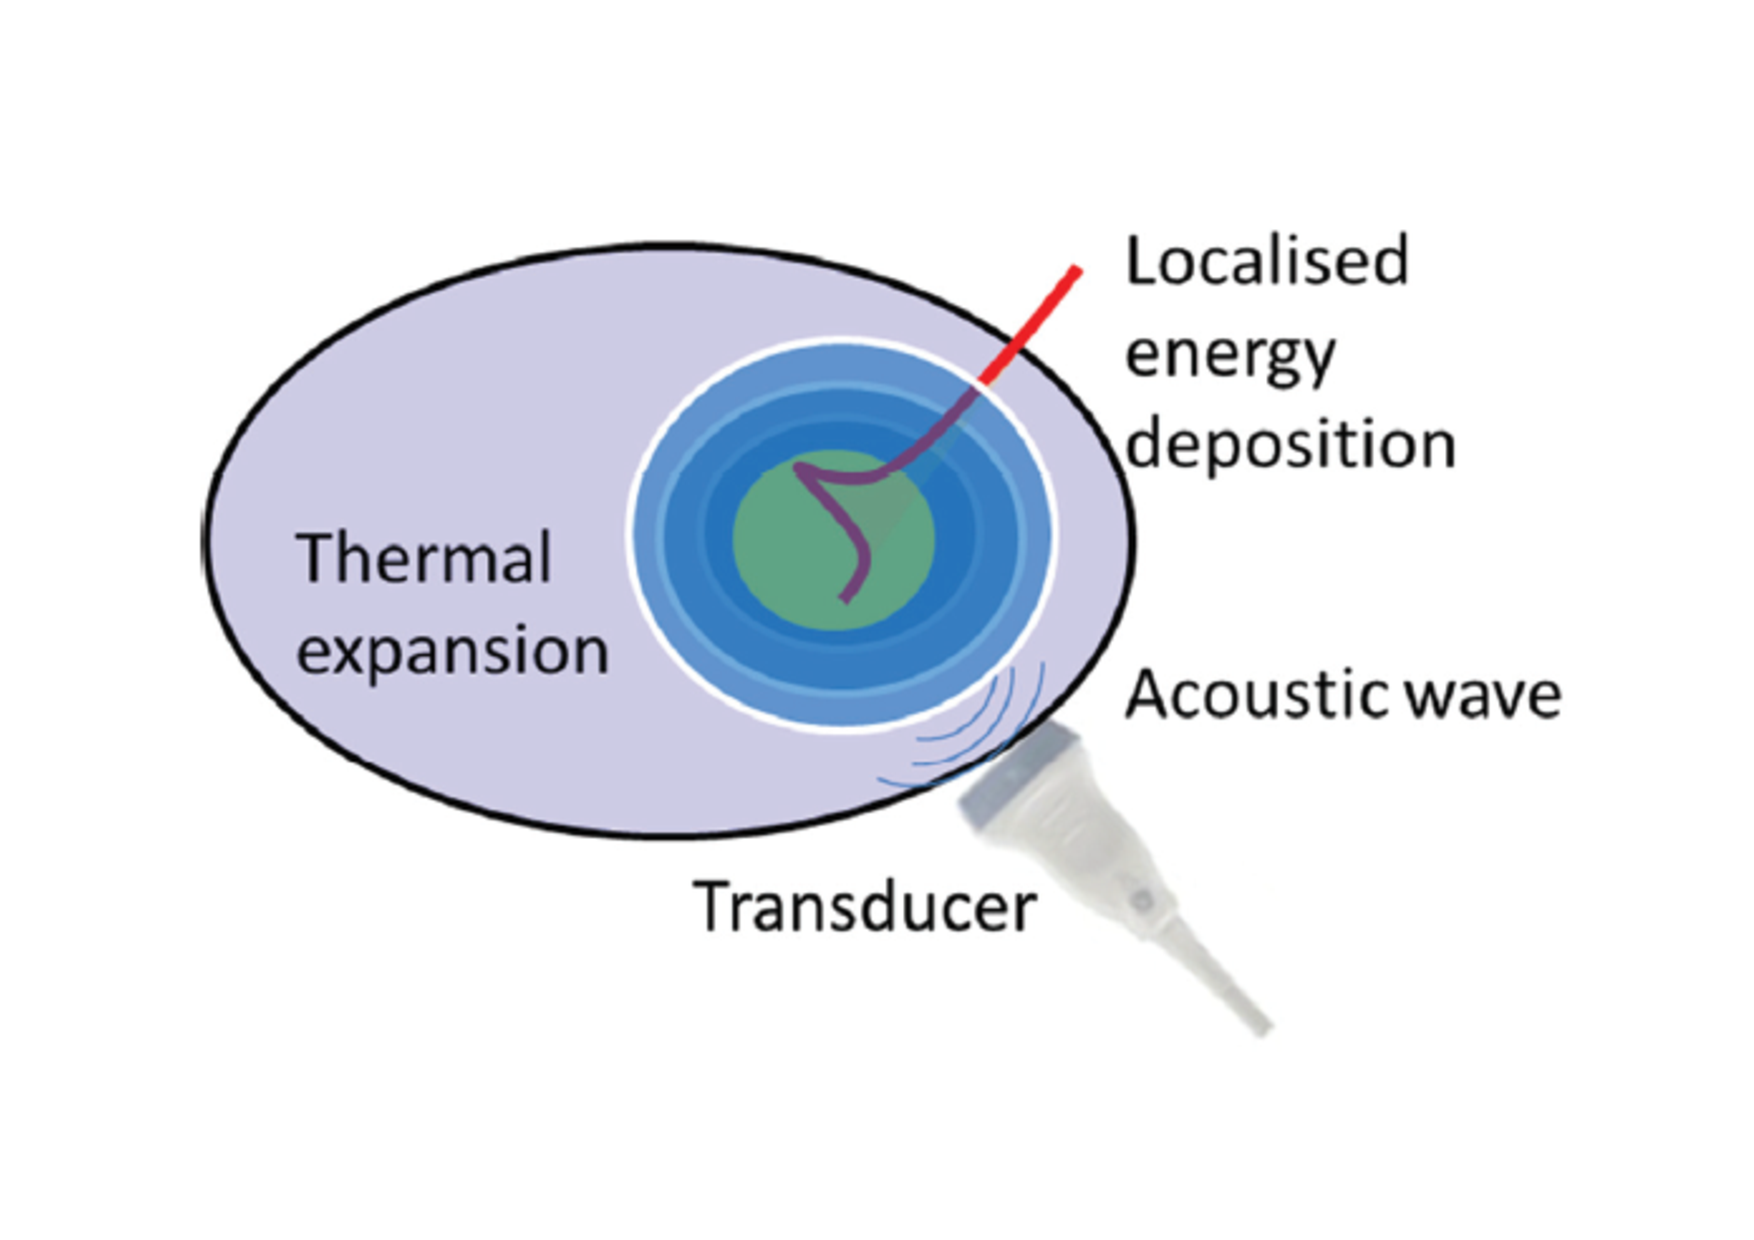
\includegraphics[width=0.98\linewidth]{03_GraphicFiles/chapter1_Introduction/ionoacoustic.pdf}
\caption{Schematic view of the basic principle of iono-acoustic waves detection for ion range verification. In~\cite{Parodi2015b}.}
\label{chap1::fig::ionoacoustic}
\end{subfigure}
\begin{subfigure}[t]{.49\textwidth}
\centering
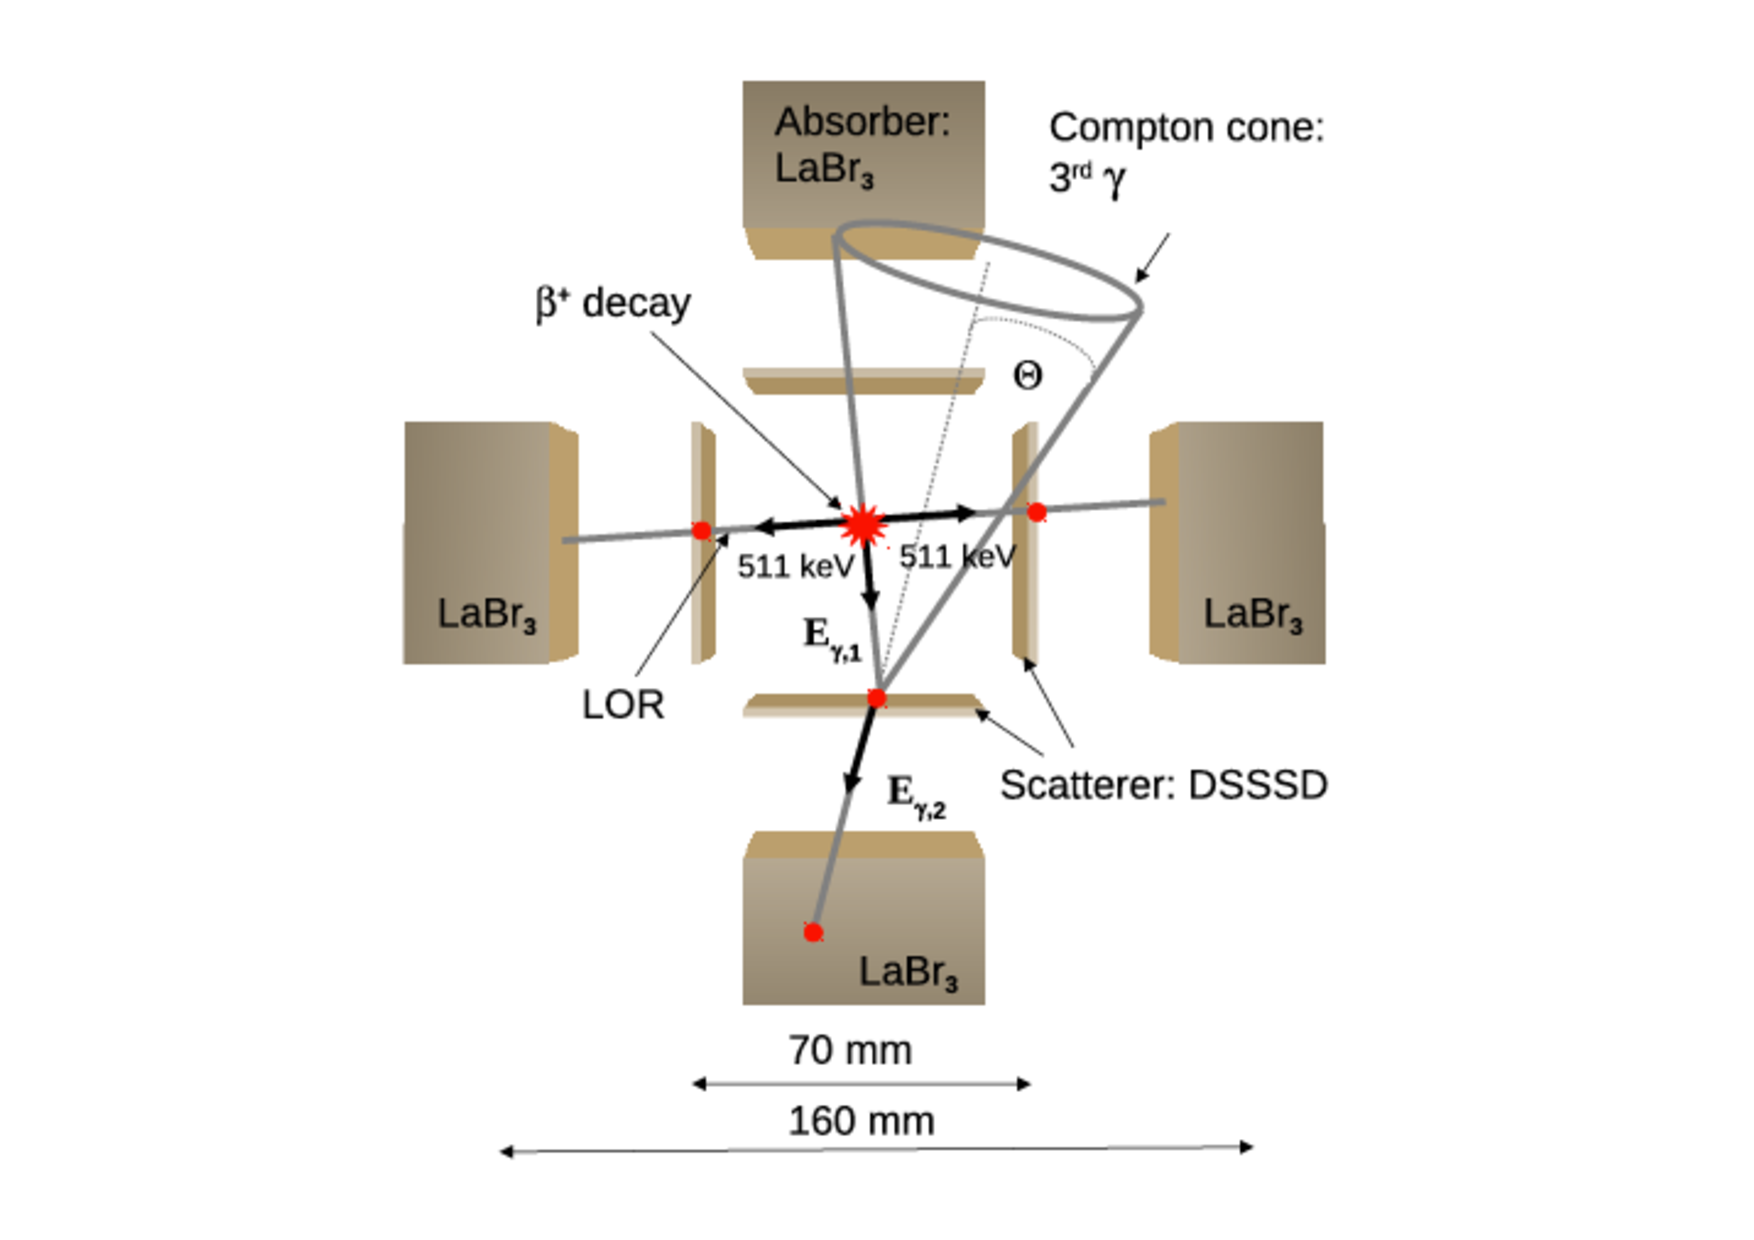
\includegraphics[width=0.92\linewidth]{03_GraphicFiles/chapter1_Introduction/3gamma.pdf}
\caption{Conceptual design of the 3-$\gamma$ detection system proposed in~\cite{Lang2014}, composed of multiple Compton camera arms for the detection of correlated \gls{pet} and de-excitation gammas or \gls{pet} and prompt photons produced in nuclear interactions during particle therapy treatments. In~\cite{Lang2014}.}
\label{chap1::fig::3gamma}
\end{subfigure}
\caption{Alternative methods for in-vivo range verification of ion beam therapy include the detection of iono-acoustic waves produced by the localized dose deposited by the energetic ion beams, whose principle is sketched on the left side, and hybrid systems for 3-photon detection, which can be applied to both nuclear medicine diagnostics and hadrontherapy monitoring, as the one sketched on the right side.}
\label{chap1::fig::alternativeRange}
\end{figure} 

Also water luminescence effects have been verified during the irradiation \myMarginnote{Water luminescence} with proton pencil beams, and are under investigation as a promising solution for range and field width estimations~\parencite{Komori2018}.   
As mentioned, the listed methods have been proposed as alternatives with respect to the more investigated detection of secondary emitted photons, both from positron annihilation and prompt-emission. These two techniques are anyway the most advanced ones, and also hybrid systems are under investigation to obtain a combination of their main advantages and a potential reduction of the identified drawbacks\myMarginnote{Hybrid systems}.  
The so-called \enquote{3-$\gamma$} imaging concept has been explored in France and Germany. The French group combined a standrd full ring \gls{pet} scanner with a time projection chamber filled with liquid xenon for the Compton measurement~\parencite{Oger2012}, while the German one focused on multiple Compton camera heads for the detection of the three $\gamma$s~\parencite{Lang2014}. This system, although originally designed for the detection of positron annihilation photons and correlated de-excitation rays for nuclear medicine application, can be adapted to performe combined detection of 511~keV photons from $\beta^+$ emission and \glspl{pg}, as already highlighted in~\parencite{Lang2014}. A conceptual detector design for such an applications shown in \figurename~\ref{chap1::fig::3gamma}. Another interesting simulation study applying this \enquote{whole-gamma imaging} concept in nuclear medicine is reported in~\parencite{Yamaya2017b}. 
Further information about hybrid systems can be found in chapter~\ref{chap::2} for what concerns the application in ion range verification and in section~\ref{chap1::subsec::Hybrid_NM} for the investigation devoted to the nuclear medicine field.

\newpage

\section{Nuclear medicine}\label{chap1::sec::NuclearMed}

Nuclear medicine is a medical specialty which makes use of particle physics concepts (in addition to medical, biological and chemical knowledge) and instrumentation to study physiological processes and perform non-invasive diagnostic examinations and disease treatments. More specifically, nuclear medicine groups all the medical techniques which foresee the use of chemical compounds containing a radioactive isotope; this radio-pharmaceutical is given to the patient (or mixed to patient samples, for example blood) orally, by injection or by inhalation, and the isotope decay products are used to deliver a treatment dose, for example to cancerous tissues, or for imaging purpose, in case the emitted particles can exit the body and be detected by radiation detectors. 
This thesis focuses on the development of gamma detectors, originally designed for the application in particle therapy; the following sections are devoted to delineate the context in which the studied detectors can be applied for diagnostics, and simulation results of such an application are reported in chapter~\ref{chap::5}.

Some hints about the historical origins of this medical fields have been given in the introduction of this chapter. The use of radioactive isotopes for medical purposes has been investigated since 1920, at the beginning only theoretically, then, since 1940, attempts have been undertaken at imaging radio-nuclide concentration in the human body. The first scan of a radio-nuclide activity in the body was obtained with a very slow planar scanner introduced by Ben Cassen at the beginning of the fifties~\parencite{Blahd1996}, and less then 10 years later Hal Anger developed the first gamma camera, introducing the approach still followed for the modern detectors~\parencite{Anger1958}. The Anger scintillation camera is a planar physically collimated detector which produced two-dimensional projection images of the radio-isotope activity without scanning. The Anger camera, if rotated around the patient, can also be used for tomography, with reconstruction algorithms able to reproduce the three-dimensional emission distribution from two-dimensional multiple-angle slices. The method to reconstruct images from projections had been published by Radon in 1917~\parencite{Radon1917}, and then applied in \gls{ct} and nuclear medicine after 1970. Iterative reconstruction methods were also being investigated, but their application started in the eighties when more computer power became available. The tomographic translation of the Anger gamma camera determined the born of \gls{spect} imaging: together with \gls{pet}, \gls{spect} is still the basis of present diagnostic nuclear medicine. The idea of detecting photon pairs produced by positron annihilation is also attributed to Anger, but the first dedicated \gls{pet} system was built by Ter-Pogossian and colleagues in the 1970s, and employed for phantom and animal studies~\parencite{Ter-Pogossian1975, Ter-Pogossian1983}. Soon afterwards, Phelps, Hoffman and colleagues built the first whole-body \gls{pet}-scanner~\parencite{Hoffmann1976}. 
In the next sections, the physics of radioactive decays is briefly reminded to introduce the detailed discussion of \gls{pet} and \gls{spect} techniques, including a short historical overview, the presentation of the imaging principle and an overview of state-of-the-art machines.
   
\subsection{Radiotracers}\label{chap1::subsec::NMradionuclides}

Nuclear medicine imaging techniques are based on radio-tracers. A tracer is a chemical compound which transports an unstable isotope (radio-nuclide); this molecule is designed to be involved in specific metabolic processes and, thus, to concentrate in the area to be targeted for imaging purpose. The $\gamma$-rays emitted by the radio-nuclide can be measured as a function of position and time, providing anatomical and metabolic information.  In the following, the main physical aspects of radioactive decays are briefly recalled. 

As mentioned, a radio-nuclide is an unstable isotope of a chemical element which decays towards a stable atomic configuration and loses energy by emitting radiation in the form of particles and electromagnetic rays. The decay can involve several steps, if the resulting \enquote{daughters} are still unstable, and the process continues until a stable nuclide is reached. 
Some general features of radioactive decay processes can be detailed mathematically without regard to a specific mechanism. In particular, the decay rate of a sample of radioactive nuclides depends on the nuclides population $N$, according to a decay constant noted as $\lambda$, as expressed by equation~\ref{chap1::eq::decayRate}. 

\begin{equation}\label{chap1::eq::decayRate}
\frac{\mathrm{d}N}{\mathrm{d}t} = -\lambda N 
\end{equation} 

On one hand, the decay constant $\lambda$ is specific of each nuclide, and reflects its degree of instability. The decay rate, on the other hand, is a representation of the sample activity, which is measured in the \gls{si} in Bequerel (1 Bq = 1 disintegration per second) and its multiples, even if an older and still used unit is the curie (Ci) (1 Ci = 3.7 $\times$ 10$^{10}$ disintegration per second). The solution of the differential equation in~\ref{chap1::eq::decayRate} gives the number of parent atoms $N$ at any time $t$, or the activity by multiplying both side by $\lambda$:

\begin{equation}\label{chap1::eq::parentAtoms}
\begin{split}
N = N_{0}e^{-\lambda t}  \\
A = A_{0}e^{-\lambda t}  \\
\end{split}
\end{equation} 

with $N_0$ and $A_0$ the original number of parent atoms and the original activity, respectively. Following these first expressions, the physical half-life $T_{1/2}$ of a radioactive nuclide is the time required for the decay of half of the atoms in a sample; its mathematical form is reported in equation~\ref{chap1::eq::half-life}.

\begin{equation}\label{chap1::eq::half-life}
T_{1/2} = \frac{\mathrm{ln}2}{\lambda} = \frac{0.693}{\lambda}
\end{equation} 

Several decay modes exist, and they can be divided into three main categories: emission or capture of nucleons (protons and neutrons), emission or capture of $\beta$-particles (electron and positrons), emission of photons. In particular, five main decay channels have been identified:
\begin{itemize}
\item $\alpha$-decay;
\item electron emission - $\beta^-$-decay;
\item electron capture;
\item positron emission - $\beta^+$-decay;
\item isomeric transition.
\end{itemize}
In \figurename~\ref{chap1::fig::decayScheme} the decay scheme of a generic nuclide $^{A}_{Z}X$ is depicted (A is the atomic mass, Z the number of protons); the $\alpha$-decay produces $^{A-4}_{Z-2}P$, electron capture and positron emission equivalently generate $^{A}_{Z-1}Q$, while $^{A}_{Z+1}R$ originates from electron emission and can be created in a metastable configuration $^{A}_{Z+1}R^*$ which then decays to the stable state via isomeric transition with the emission of a photon.  

\begin{figure}[!htbp]
\begin{subfigure}[t]{.35\textwidth}
\centering
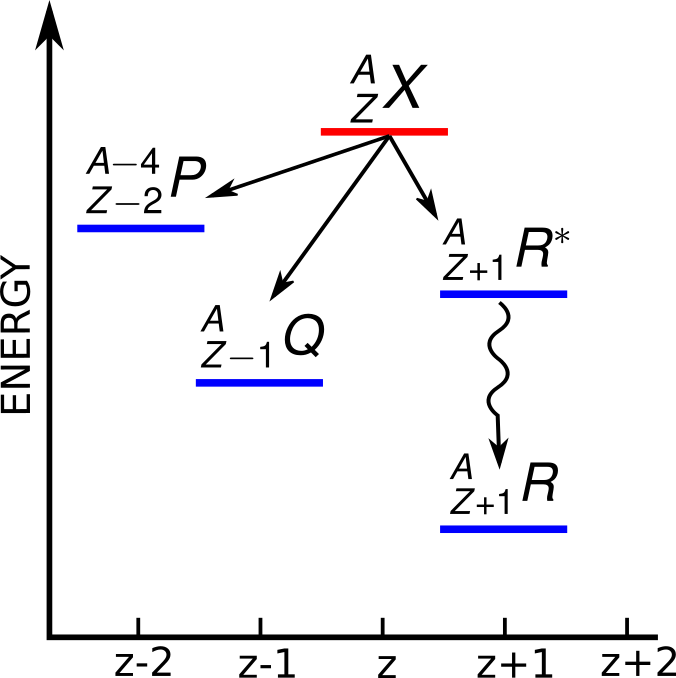
\includegraphics[width=0.9\linewidth, trim={0 4cm 0 3cm}, clip]{03_GraphicFiles/chapter1_Introduction/decayScheme.pdf}
\caption{Radioactive decay scheme. In~\cite{Hendee2002}}
\label{chap1::fig::decayScheme}
\end{subfigure}
\begin{subfigure}[t]{.64\textwidth}
\centering
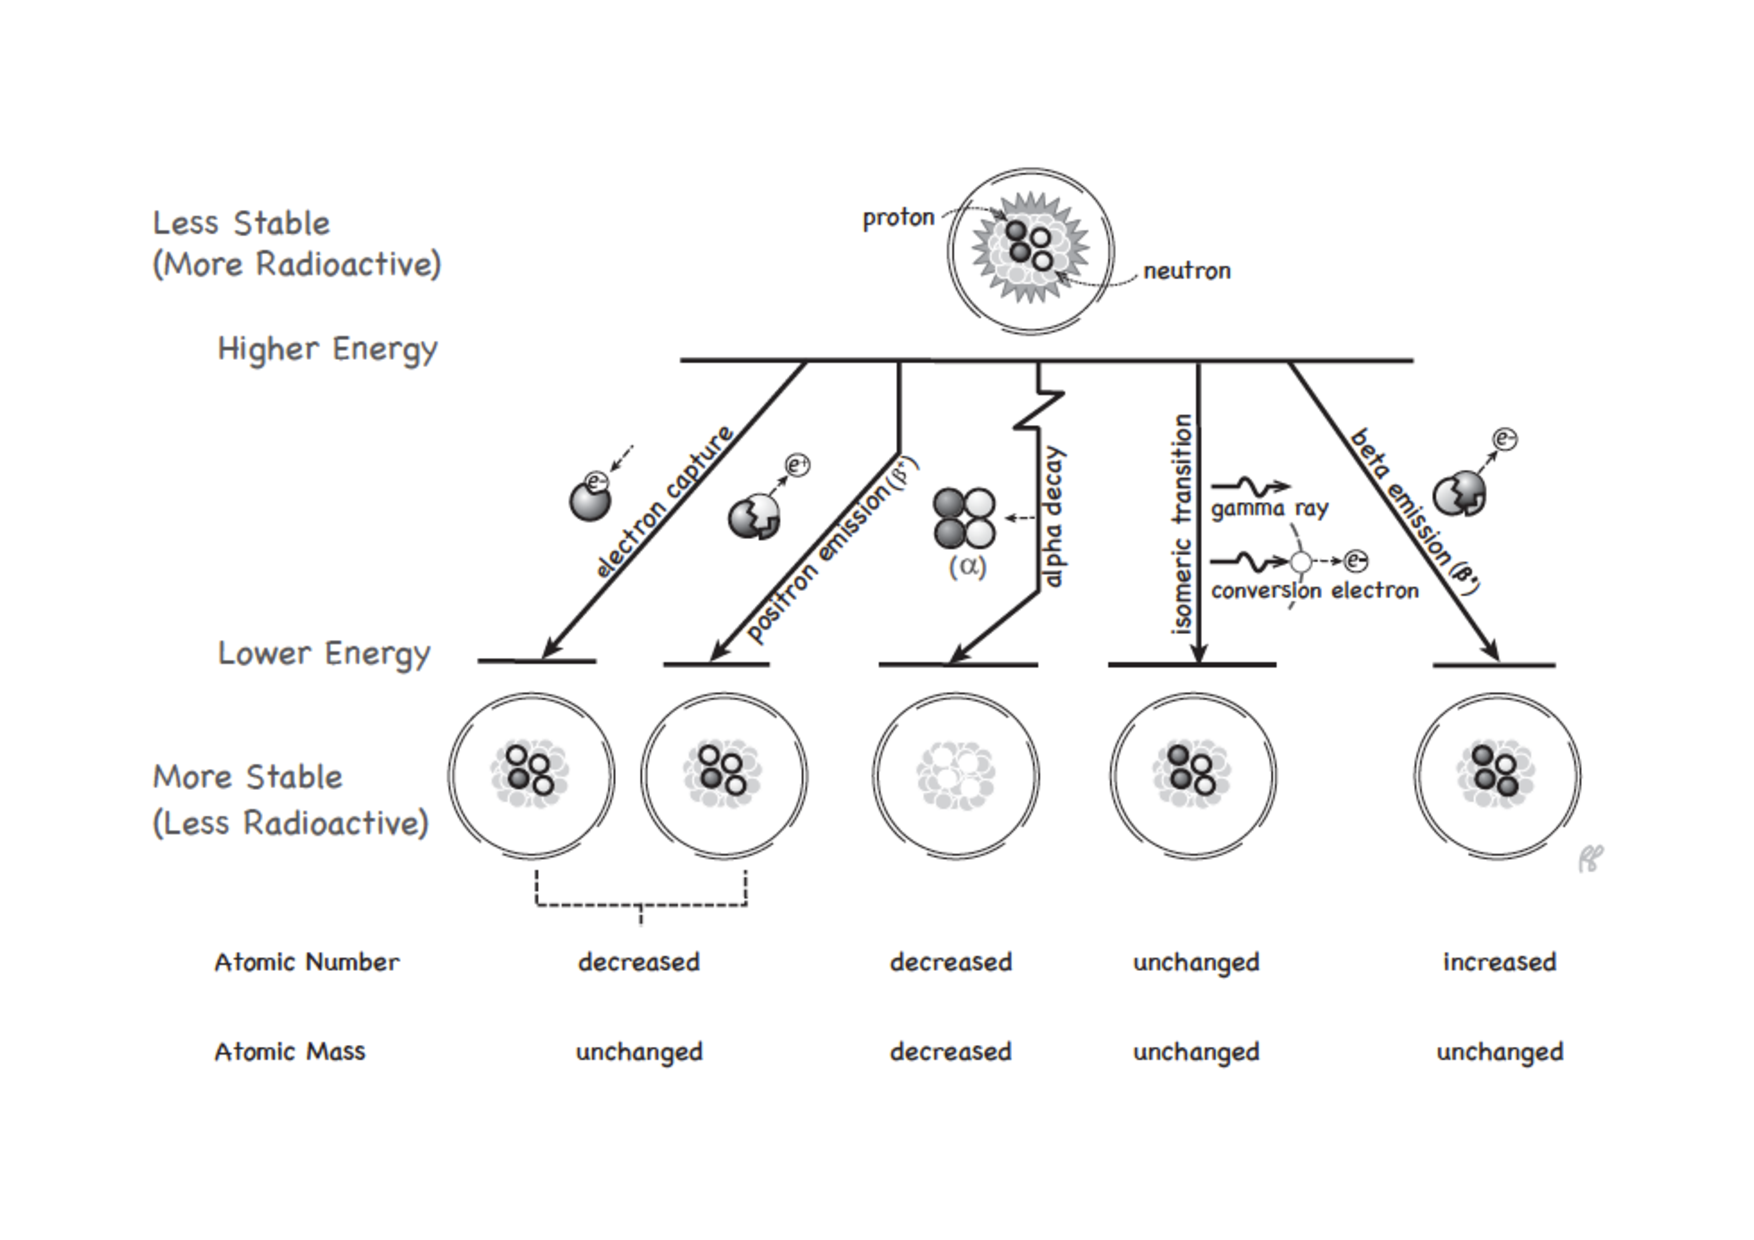
\includegraphics[width=0.98\linewidth]{03_GraphicFiles/chapter1_Introduction/decaySchematicSimple.pdf}
\caption{Schematic view of the radioactive decays. In~\cite{Powsner2013}.}
\label{chap1::fig::nuclides}
\end{subfigure}
\caption{The various radioactive decay channels are schematized in (a) for a generic isotope $^{A}_{Z}$X. A more detailed scheme, describing the decay processes and products, is given in (b).}
\label{chap1::fig::radioactiveDecay}
\end{figure} 

The $\alpha$-decay \myMarginnote{$\alpha$-decay} is the spontaneuous emission of an $\alpha$ particle (i.e. an helium nucleus, consisting of two protons and two neutrons), typically from heavy nuclides (A > 150). It was discovered by Marie and Pierre Curie in 1989~\parencite{Curie1898} and first described by Rutherford one year later~\parencite{Rutherford1899}, who also identified the $\alpha$ particles as helium nuclei, together with Boltwood in 1911~\parencite{Boltwood1911}. The decay can be described by equation~\ref{alphaDec}. Often it is followed by the emission of characteristic x-ray or gammas, accompanied by competing processes of internal conversion and Auger electron emission. The produced $\alpha$ particles have energies in the range 2-10~MeV and are not used for imaging purposes, given the very limited range in tissues (about 100~\charmu ~m). This characteristic makes such a decay appropriate for therapy, even if the very short decay time is a limiting factor. Only the $\alpha$-decay of a few high-Z elements is actually used, for example, for tumor irradiation in the so-called \enquote{internal radiotherapy} or \enquote{brachytherapy}~\parencite{Suntharalingam2005, Dahiya2016}. 

\begin{equation}\label{chap1::eq::alphaDec}
^{A}_{Z}X \, \rightarrow \, ^{A-4}_{Z-2}Y + ^{4}_{2}\mathrm{He} + \mathrm{energy}
\end{equation} 

The decay via emission of an electron \myMarginnote{Electron emission} ($\beta^-$- or negatron-decay) can be seen as the conversion of a neutron in a proton-electron pair, as in the generic reaction reported in equation~\ref{chap1::eq::electronEmiss}.

\begin{equation}\label{chap1::eq::electronEmiss}
\begin{split}
^{A}_{Z}X \, \rightarrow \, ^{A}_{Z+1}Y + e^{-} + \overline{\nu} + \mathrm{energy} \\
n \, \rightarrow \, p + e^{-} + \overline{\nu} 
\end{split}
\end{equation}   
 
This decay channel pertains to nuclei with a N/Z ratio (with N the number of neutrons) too high for stability and results in nucleus with Z increased by one, N decreased by one and so the same atomic mass A (isobaric transition) but a different chemical element. $\beta^-$-decay pathways are characterized by specific maximum energies $\mathrm{E_{max}}$, but in most of the cases the emitted electron energy is lower than the maximum, with an average value of approximately 1/3 $\mathrm{E_{max}}$, and the remaining energy is carried away by the anti-neutrino. This results in poly-energetic energy spectra for the emitted electrons. The difference in the energy released during decay and the one possessed by the emitted electron threatened the energy conservation law for years. In 1930, in a letter, Wolfgang Pauli suggested that a second particle was emitted during the decay, explaining the energy, momentum and angular momentum conservation. The name neutrino was attributed to such a particle by Enrico Fermi. 
Any possible excess energy in the nucleus after the decay (metastable state) is emitted as gamma rays or internal conversion electrons. As for the $\alpha$ particle case, electrons have limited range in matter, thus release dose to the tissues, and have no diagnostic value (but they are used in brachytherapy), but metastable states deriving from $\beta^-$-decays are pure sources of $\gamma$-rays and are so employed for imaging. One of the most diffused tracer is a metastable daughter of $^{99}$Mo, the $^{99m}$Tc; it decays in stable $^{99}$Tc (half life = 6 hours) by emitting a 140~keV photon.   

On the other side of the \enquote{nuclide stability line}, \myMarginnote{Positron emission} neutron-poor radionuclides (with low N/Z ratio) tend to decay by the emission of a positron ($\beta^+$ decay) and to increase the neutron number by one. As shown by equation~\ref{chap1::eq::positronEmiss}, the net result is the conversion of a proton into a neutron with the ejection of a neutrino, in addition to the positron. As in the previous case, the transition is isobaric because the total number of nucleons is unchanged.

 \begin{equation}\label{chap1::eq::positronEmiss}
\begin{split}
^{A}_{Z}X \, \rightarrow \, ^{A}_{Z-1}Y + e^{+} + \nu + \mathrm{energy} \\
p \, \rightarrow \, n + e^{+} + \nu 
\end{split}
\end{equation}     

The emission of positrons was discovered in 1933 by the Marie Curie daughter Irene Curie and her husband Frederic Joliet, in bombardments of aluminium by $\alpha$ particles~\parencite{Leone2010}. Even if the reaction principle is similar to $\beta^-$-decay, an important difference resides in the behavior of the decay product. Both electron and positron undergo energy deposition processes by excitation and ionization, but if electrons can be captured by atoms (or absorbed in free electron bands) when they come to rest, positron react with their antiparticle (electron) by annihilation. The entire rest mass of the particle pair is converted to energy and emitted as two back-to-back 511~keV photons for conservation laws. The annihilation takes place in a time window of about 1~ns after the $\beta^+$-decay, and within a few millimeter of the decay site (depending on the medium). This kind of reaction is the basis of one of the most diffused nuclear medicine imaging technique, the \gls{pet}, discussed in section~\ref{chap1::subsec::PET_NM}. An example of a positron emitter used in imaging is $^{18}$F, with a half-life of 109 minutes.
To be noticed that, as for $\beta^-$-decay, the daughter nucleus can further emit photons to lower its energetic level, which can be used in combined imaging techniques (three-$\gamma$ imaging).
The N/P ratio of neutron deficient nuclides can also be increased via \gls{ec} reactions \myMarginnote{\gls{ec}}; the nucleus can capture and orbital electron and convert a proton into a neutron, with the consequent emission of a neutrino. This phenomenon is described by equation~\ref{chap1::eq::electronCapture}.

 \begin{equation}\label{chap1::eq::electronCapture}
\begin{split}
^{A}_{Z}X + e^{-} \, \rightarrow \, ^{A}_{Z-1}Y  + \nu + \mathrm{energy} \\
p + e^{-}\, \rightarrow \, n  + \nu 
\end{split}
\end{equation}     

Most electrons are captured from the K shell, more uncommon are the capturing processing involving L shell or even shells farther from the nucleus. As a result of the capture, a vacancy is created and filled by an electron from an higher-energy shell. This transition leads to a reduction of the atomic rest energy, and the release of characteristic x-rays and/or Auger electrons. As with other modes of decay, further $\gamma$-rays can be emitted if the daughter nucleus is left in an excited state after the capture process. An example of electron capture decay is represented by $^{201}$Tl, which decays to $^{201}$Hg with the emission of K-x-rays of 69-83 keV (98\% abundance) and $\gamma$-rays of 135 and 167~keV in 10\% total abundance. Many nuclei decay by both electron capture and positron emission , as for example the $^{22}$Na.
As mentioned for the previously described decay modes \myMarginnote{Isomeric transition - $\gamma$-decay}, often the daughter nucleus is formed in an excited state, which is still unstable. The transition towards a condition of stability entails an internal atomic re-arrangement and the emission of $\gamma$-rays at characteristic energies. In general, such a transition is almost instantaneous, but some excited states can persist for longer periods, with half-lives which ranges on several orders of magnitude, between 10$ˆ{-6}$~s and hundreds of years. The decay of this kind of nuclei, called metastable or isomeric, is called isomeric transition, and only results in the $\gamma$-ray emission with no emission or capture of other particles by the nucleus. A complementary pathway for the energy release is represented by the interaction of the nucleus with an atomic electron; this process is called \gls{iconv}, and the involved electron is ejected. This emission is further followed by x-rays and Auger electron emission, so that the atom can resume a stable state. The isomeric transition is described by equation~\ref{chap1::eq::isomericTrans}, where the letter m indicates the metastable state.

 \begin{equation}\label{chap1::eq::isomericTrans}
^{Am}_{Z}X  \, \rightarrow \, ^{A}_{Z}X  + \mathrm{energy} \\
\end{equation}        

To be noticed that no radioactive nuclide decays solely by an isomeric transition, which is always preceded by another decay mode. In addition to the already mentioned decay of $^{99m}$Tc, deriving from the previous decay of $^{99}$Mo, also $^{60}$Co decays in excited $^{60}$Ni nuclei which then reach the ground energy state by isomeric transition and with the emission of 1.17 and 1.33~MeV photons. 
In table~\ref{chap1::tab::Isotopes_NM} some of the radioisotopes typically used for imaging and therapy are listed with their half-life and common uses. 

\begin{table}[!htbp]
\centering
\caption{Commonly-used radioisotopes for the clinical imaging and therapy routine. Table adapted from~\cite{Ruth2009}.}
\label{chap1::tab::Isotopes_NM}
\resizebox{\textwidth}{!}{%
\begin{tabular}{clll}
\toprule
\rowcolor{myColorMainA!20} 
\textbf{Application} & \textbf{Radioisotope}& \textbf{Half-life} & \textbf{Details} \\
\midrule
\multirow{12}{*}{\STAB{\rotatebox[origin=c]{90}{Imaging}}}& Technetium-99m & 6 h (from $^{99}$Mo 66 h)    &  Used to image the almost all the body, skeleton and heart muscle in particular.\\
& Cobalt-57             & 272 d                                        & Used as marker to estimate organ size and for \textit{in vitro} diagnostic kits.\\
& Gallium-67           & 78 h               						    & Used for tumor imaging and localization of inflammatory lesions.\\
& Indium-111           & 67 h     								    & Used for specialist diagnostic studies and colon transit studies.\\
& Iodine-123           & 13 h      								    & Used for diagnosis of thyroid function.\\
& Krypton-81m       & 13 s (from $^81$Rb 4.6 h)	    & Used in gas status for images of pulmonary ventilation and in general for lung applications.\\
& Rubidium-82       & 65 h          							    & Convenient \gls{pet} agent for myocardial perfusion imaging.\\
& Thallium-201       & 73 h  									    & Used for diagnosis of coronary artery disease and other heart studies.\\
& Carbon-11           & 20.4 m 								    & \\
& Nitrogen-13        & 9.97 m  								    & Positron emitters used in \gls{pet} for studying brain physiology and pathology.\\
& Oxygen-15          & 2 m    								        & They also have a significant role in cardiology.\\
& Fluorine-18         & 110 m									   & \\ 
\midrule
\multirow{4}{*}{\STAB{\rotatebox[origin=c]{90}{Therapy}}}& Bromine-77         & 2.4 d                                            & Auger electrons decay mode.\\
& Palladium-103     & 17.5 d                                          & Auger electrons decay mode.\\
& Rhenium-186      & 90.6 h                                         & $\beta^-$-decay mode.\\
& Astatine-211       & 7.2 h               						   & $\alpha$-decay mode.\\
\bottomrule
\end{tabular}}
\end{table}    

Although many naturally occurring radioactive nuclides exist \myMarginnote{Radionuclide production}, all of those commonly administrated to patients in nuclear medicine tracers are produced artificially in order to fit the clinical requirements. Artificial induced radioactivity was introduced by the already mentioned Irene Curie and his husband, who bombarded aluminum targets with $\alpha$ particle~\parencite{Leone2010}. Nowadays, most radionuclides are produced with cyclotrons, nuclear reactors or radionuclide generators. In general, $\beta^-$ emitters are produced by bombarding stable nuclei with neutrons from nuclear reactors, while $\beta^+$-decay nuclides are produced with bombardment with protons, helium ions, deuterons or tritons accelerated with cyclotrons (see section~\ref{chap1::subsubsec::accelerators} for the description of the cyclotron). In other cases, radionuclides are produced as by-products of fission in nuclear reactors, or as decay product of other isotopes produced with one of the listed methods. 
In the cyclotron-based production, the accelerated ions collide with the target nuclei causing nuclear reactions, presented in section~\ref{chap1::subsubsec::ionInteractions}. As explained, fragmentation processes can create radioactive nuclei, such as $\beta^+$ emitters, employed in \gls{pet} diagnostics. In general, cyclotron facilities must be in close proximity to the hospital where the produced radionuclides will be administrated because of their short half-life. $^{18}$F, created with this technique as product of nuclear reactions with $^{18}$O, is an exception in this sense, with an half-life of 109 minutes. 
In nuclear reactors, two techniques are exploited: nuclear fission and neutron activation. The absorption of neutrons from nuclear reactors can induces fission processes in heavy nuclei, which split in lighter (often unstable) ones. Its long half-life makes $^{235}$U the most widely used fissile element; when it absorbs a neutron, the resulting state of $^{236}$U is highly unstable and promptly splits into its fission fragments. For example, $^{99}$Mo has already been mentioned as the parent nucleus for the production of  $^{99m}$Tc and derives by the fission of uranium. Another widely used nuclide produced with fission procedure is the $^{131}$I. The creation of the fission fragments is very often accompanied by the emission of secondary neutrons which can be used to create other nuclides by neutron activation. Stable nuclei, indeed, can capture neutrons and produce, in most cases, $\beta^-$ emitters, as the $^{32}$P or the $^{50}$Cr. In some cases, the sample activity reached with such a production technique is not sufficient, because stable nuclei are still present among the parent atoms, and so fission mechanisms are preferred. 
The last mechanism involves radionuclide generators, particularly interesting for short half-life nuclides. In order to solve the supply problem for short-living isotopes, the sample is often prepared with the longer-living parent nuclide (the so-called \enquote{generator}), which then decays in the desired one continually providing it. This is for example the case of the most important radio-nuclide used in a variety of application, $^{99m}$Tc, result of the decay of $^{99}$Mo. 

Once produced, the radioactive nuclei must be attached \myMarginnote{Radiotracer features} to appropriate substances providing the desired biological properties, for example to be preferentially absorbed in the target region. The final product, ready to be administrated to the patient, is called \enquote{radiotracer}. 
For diagnostics, the selected radioisotope half-life should be short enough so that a considerable part of the decays occurs during the examination time; any radiation released after the end of the examination is a source of useless dose to the patient. The dose delivered after the end of the treatment can be reduced if the biological excretion, guaranteed by the tracer characteristics, is rapid. Always focusing on diagnosis, the optimal decay scheme is the pure $\gamma$-decay, with an isomer as radionuclide; anyway, the amount of produced non-penetrating radiation should be minimized. The exception is represented by $\beta^+$ emitters, resulting in the positron annihilation 511~keV photons exploited by \gls{pet} techniques. In addition to this, the produced photon energy must be considered: nowadays, the majority of scintillation cameras are optimized for energies close to 140~keV (main emission of $^{99m}$Tc), which is a compromise among patient attenuation, spatial resolution and detection efficiency. Photons at lower energies are largely attenuated by dose and increase the patient dose without contributing to the image formation. High-energy photons escape the body and deliver a minimal dose to the patient, but the present machines have poor detection efficiency in such an energy range, and the physical collimators are not optimized; both these factors result in image quality degradation. High-energy photons can be used if new detector solutions are explored, like the one presented in chapter~\ref{chap::5}. 
For therapy non-penetrating radiation are requested and must be maximized, and correlated photon emission can be in principle used for dosimetric verification, in the so-called theranostics approach~\parencite{Yordanova2017}. 
From the biological point of view, \enquote{hot spots} (in which the tracer is more concentrated then in other regions) are desired for therapy, while for diagnosis it is possible to profit from both \enquote{hot} and \enquote{cold spots} {in which the tracer is more concentrated then in other regions}. Several mechanisms can be implemented in order to concentrate the radiotracer in the target area. Localized administration of the radiotracer in the target region is the first option, while with active transport techniques, the tracer is concentrated into specific organ against concentration gradients thanks to cellular metabolic processes.  The glucose metabolism is also exploited, for example for the \gls{fdg} tracer used in 85\% of the \gls{pet} clinical practice. The tracer size is fundamental in techniques based on the phagocytosis by specialized cells or on traps in specific organs. Very large molecules (20-40~\charmu ~m diameter) can concentrate in capillaries with smaller diameter. An irregular diffusion through tissue membrane can also be used to identify lesions if specific tracers are employed. Chemotaxis (the movement of a cell in response to chemical stimulus) can also promote the migration and accumulation of radiotracers, for example as part of an overall inflammatory response. Moreover, some radio-pharmaceuticals are produced with specific characteristics which provide them high affinity to bind to receptor sites, for example in tumors. Finally, the blood flux can be used for blood specific studies. 

The choice of the radiotracer depends on the specific organ or region of the body to be examined and on the chosen detection technique. As already detailed, on one side \gls{pet} aims to detect the two back-to-back photons produced by the annihilation of a positron emitted by the radio-isotope and an electron of the patient body. On the other side, \gls{spect} detects single photons, and the spatial localization is given by mechanical collimation systems. In both cases, tomographic reconstruction is foreseen to obtain three-dimensional images.

The physical basis, historical development and present status of these two techniques are detailed in the following sections. In addition, the theranostics approach, aiming to perform combined diseases radiation treatment and diagnosis and/or verification imaging, is also addressed in the last section of this chapter.  
 
\subsection{Positron Emission Tomography}\label{chap1::subsec::PET_NM}

PET systems rely on the detection of annihilation gamma rays that follow positron decay of the radioisotope injected in the patient and consequent positron annihilation. The gamma rays exiting the patient body are detected in coincidence by scintillating detectors surrounding the patient, and the distribution of positron emitters is retrieved \textit{in vivo}. 
\figurename~\ref{chap1::fig::NM_PET_princ} shows the principle at the basis of \gls{pet} imaging. 

\begin{figure}[!htbp]
\centering
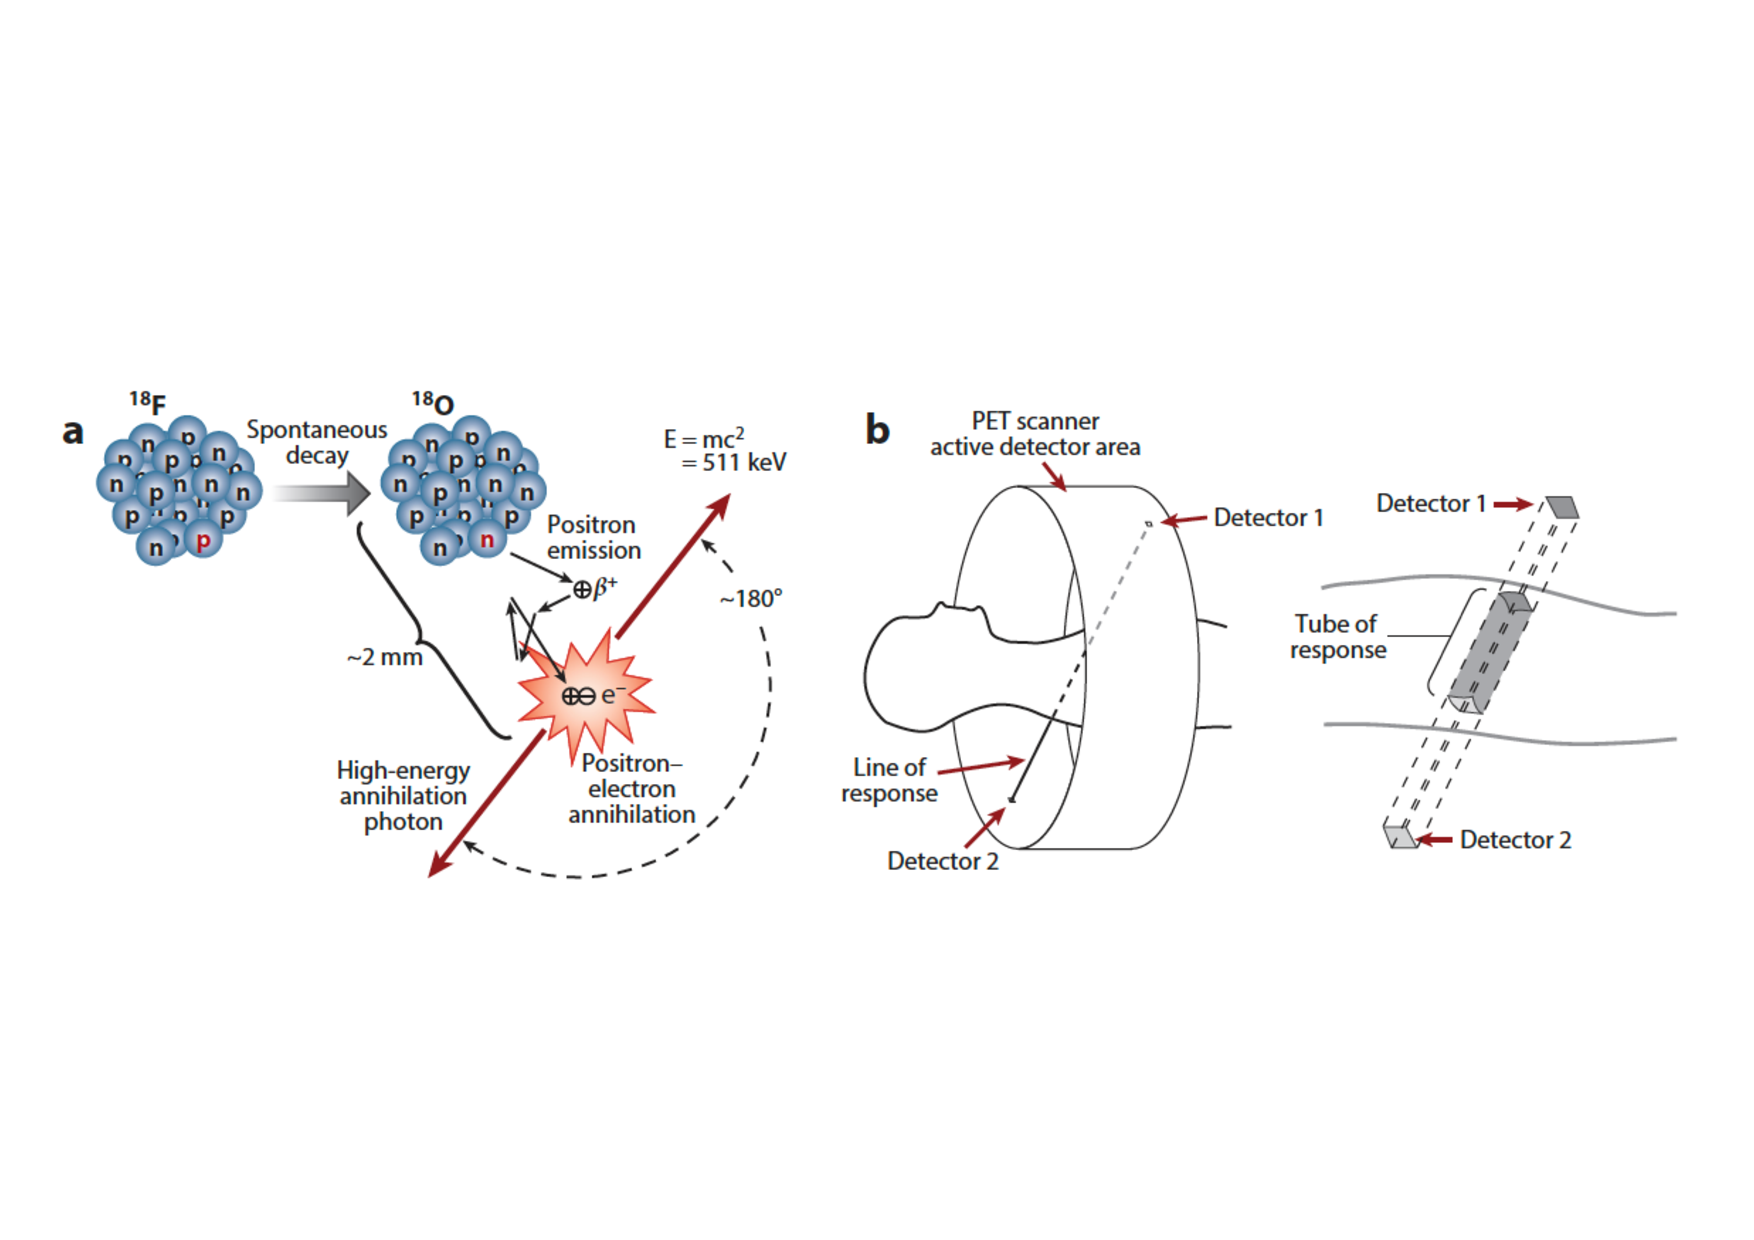
\includegraphics[width=0.8\textwidth, trim = {0 3cm 0 3cm}, clip]{03_GraphicFiles/chapter1_Introduction/NM_PET_principle.pdf}
\caption{The $\beta^{+}$ decay of $^{18}$F creates the stable isotope $^{18}$O and a positron, which travels short distance (1-2~mm) before interacting with an electron. The consequent annihilation produces two anticollinear 511~KeV photons (a). The two photons are detected by the \gls{pet} scanner in time coincidence, and the two points of interaction defines a line of response, then extended to a so-called \enquote{tube of response} which accounts for the detector's elements finite dimensions (b). In~\cite{Vaquero2015}.}
\label{chap1::fig::NM_PET_princ}
\end{figure}   
The two annihilation photons are typically detected with time coincidence windows ranging between 1 and 10~ns, depending on the specific features of the employed scanner. The spatial resolution of \gls{pet} imaging is intrinsically limited by the fundamental nature of positron annihilation, if we consider that after its creation, the positron can travel a few millimeters and follow a tortuous path through the tissue (mainly due to Coulomb scattering with electrons which can occur at large angles given the fact that the rest mass of positron is the same as the one of the electron) before reaching thermal energies and annihilating. In addition to the positron range, also the variation in the momentum of the positron leads to a limitation of the spatial resolution of \gls{pet} images. Indeed, such a variation results in an angular uncertainty in the direction of the two annihilation photons known as \enquote{noncolinearity}. Moreover, significant limitations are linked to the employed detector: the coincidence detector-pair resolution is normally specified as the \gls{fwhm} of the \gls{psf} obtained from the convolution of the two individual detector \glspl{psf}. For a detector composed of small discrete crystals, the interactions are generally assumed to take place at the center of individual crystals, and the resulting \gls{fwhm} of the coincident detector \gls{psf} is one-half the crystal size. A further factor affecting \gls{pet} imaging resolution is the parallax error, which results form the uncertainty of the \gls{doi} of the gamma rays in the crystal. Thus, unless the \gls{doi} within a crystal can be accurately determined (dedicated designs are needed), an incorrect \gls{lor} will be assigned to the interaction. A schematic representation of the parallax error is provided in \figurename~\ref{chap1::fig::PET_parallax}. The parallax error is all the more increased when the \gls{pet} ring diameter is reduced of the thickness of the crystals is increased, as the relative thickness of the detector increases. 

\begin{figure}[!htbp]
\begin{subfigure}[t]{.49\textwidth}
\centering
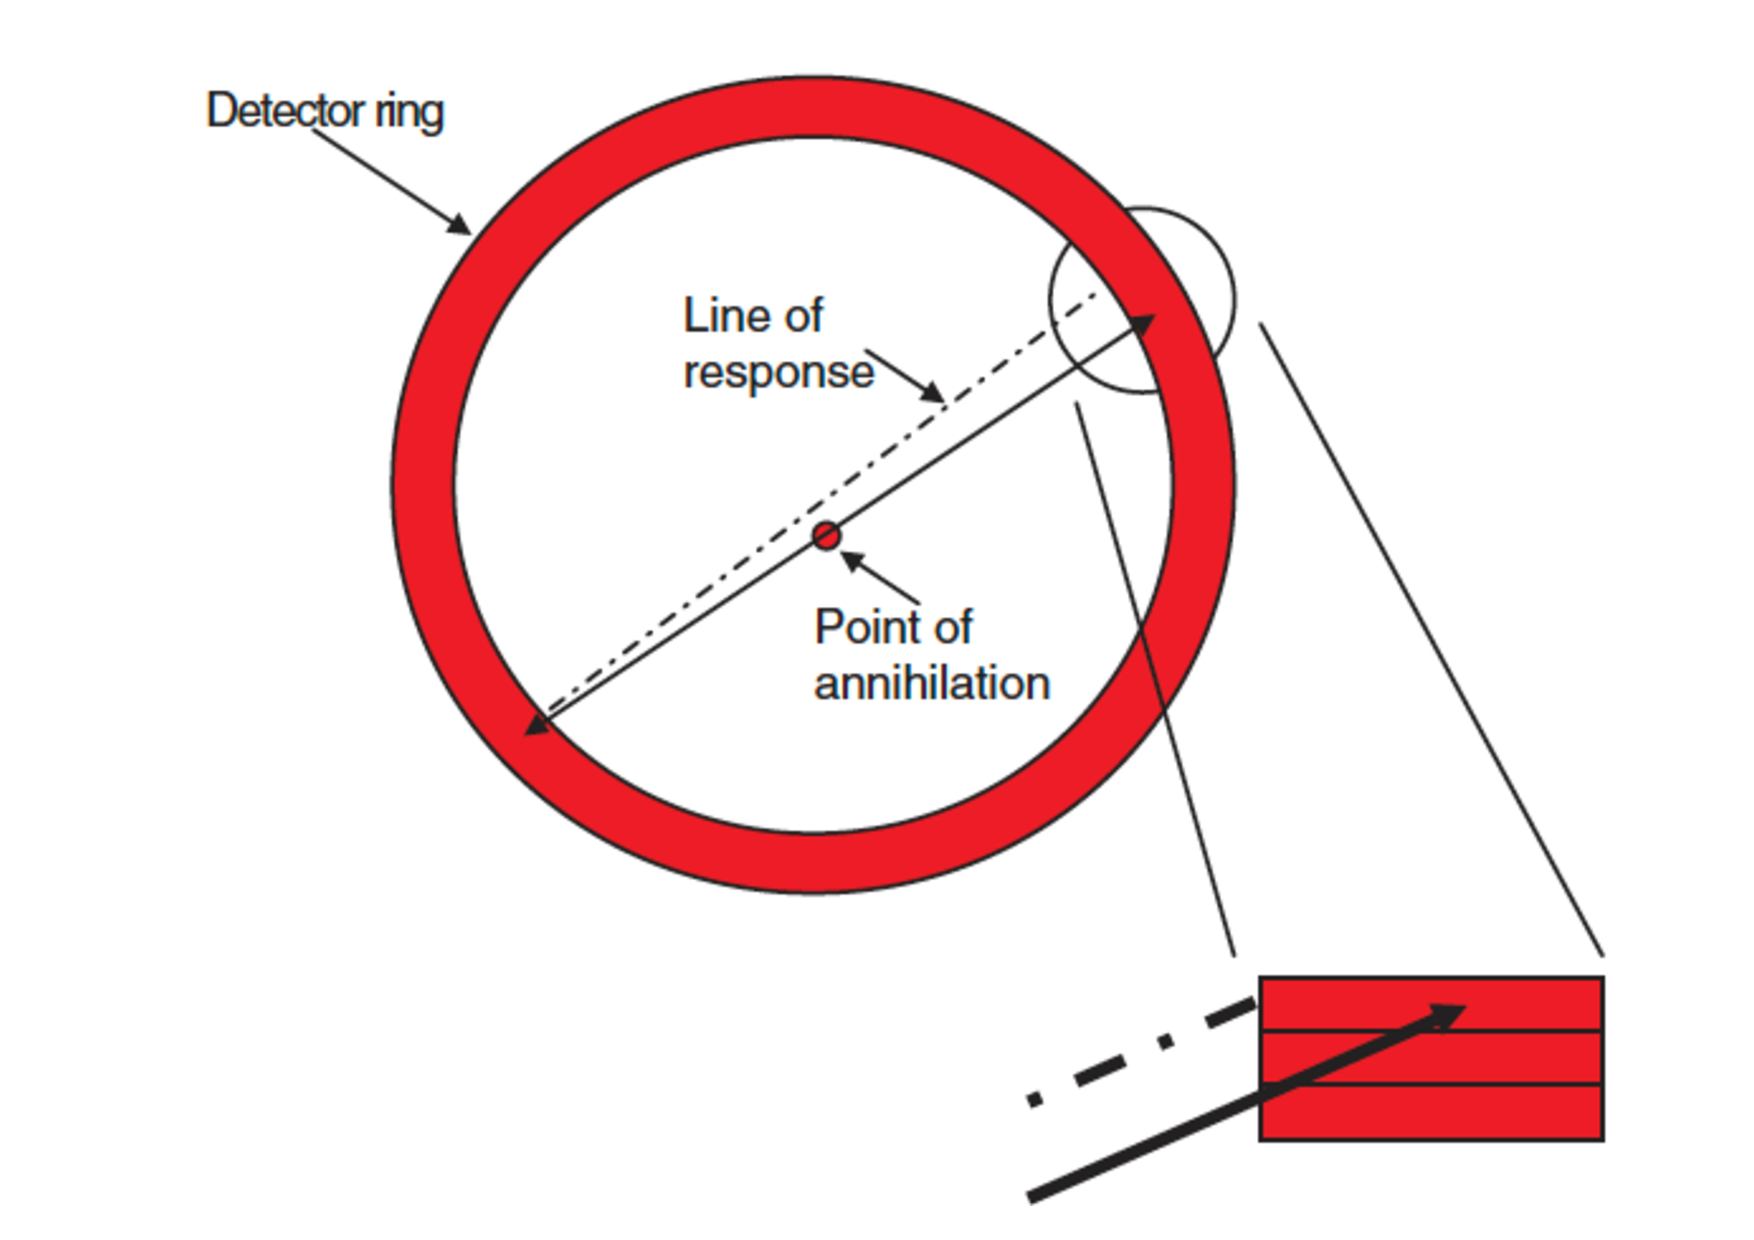
\includegraphics[width=0.7\linewidth]{03_GraphicFiles/chapter1_Introduction/PET_parallax.pdf}
\caption{Schematic view of the parallax error. The gamma ray (solid line) interacts in a crystal after penetrating one or more adjacent crystals in the detector ring. The detection electronics, if \gls{doi} information is not accessible, will incorrectly assign the \gls{lor} (dotted line) based on the front of the interaction crystal.}
\label{chap1::fig::PET_parallax}
\end{subfigure}
\begin{subfigure}[t]{.49\textwidth}
\centering
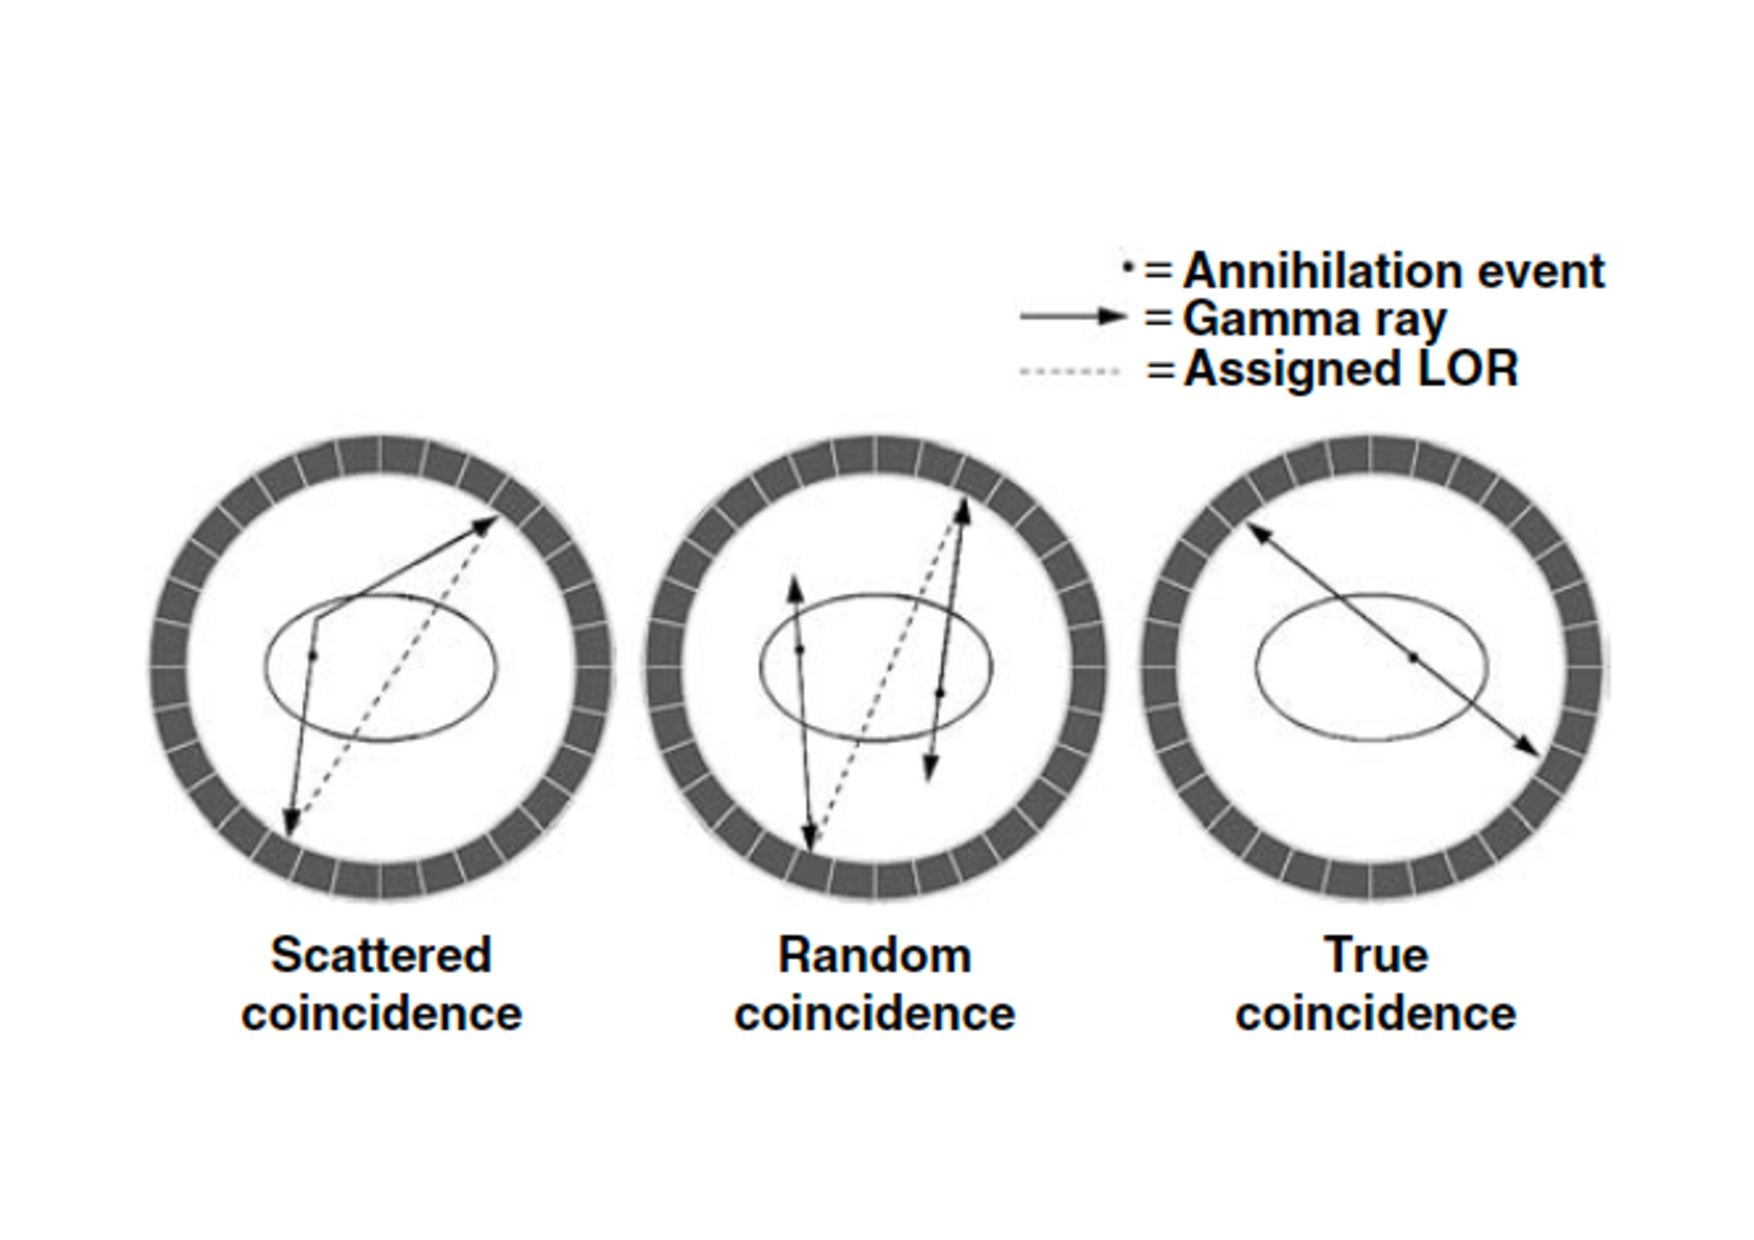
\includegraphics[width=0.98\linewidth]{03_GraphicFiles/chapter1_Introduction/PET_events.pdf}
\caption{The three types of coincidence events measured in a \gls{pet} scanner.}
\label{chap1::fig::PET_events}
\end{subfigure}
\caption{In~\cite{Lewellen2004}.}
\label{chap1::fig::PET_details}
\end{figure} 

\figurename~\ref{chap1::fig::PET_events} shows the three kinds of coincidence events that a standard \gls{pet} accepts: 
\begin{itemize}
\item true coincidences: gamma rays are detected from a single decay that have not scattered in the patient;
\item scattered events: one or both gamma rays scatter within the patient;
\item random coincidences: two separate decays result in the detection of only one gamma rays from each one and the two events are close enough in time to be in coincidence.
\end{itemize}
It is clear that increasing the number of true coincidences leads to less noise in the final image and allows one to reconstruct the collected data with high spatial resolution, and the effect of scattered coincidences can be corrected at the reconstruction stage, as well as the attenuation effect in the patient. The random coincidences are hardly treated, but their number can be reduced by decreasing the injected radiotracer activity.

The origin of the \gls{pet} imaging modality dates back to the beginning of the 50s, when a simple brain probe was used to localize brain tumors by detecting photon coincidences with 2 opposing \gls{naitl} detectors at the \gls{mgh}~\parencite{Sweet1951}. In the same year, a similar approach was published on \textit{Science} by a second reserach group~\parencite{Wrenn1951}. The development of reconstruction techniques for tomographic imaging started in the early 1960s~\parencite{Kuhl1963}, and in parallel to the first clinical trial for x-ray computed tomography the \gls{mgh} physics group developed the \gls{fbp} technique~\parencite{Chesler1971}. The first ring tomograph was built in 1973 by Robertson of \gls{bnl}, and it was composed of 32 detectors disposed in a circular array~\parencite{Robertson1972}. One year later, the PETT I (Positron Emission Transaxial Tomography) tomograph prototype was built at the Washington University by Michael E. Phelps: such a prototype was then upgraded until a human-size system, called PET III, which included extended reconstruction not limited to the transaxial plane. The system consisted of an hexagonal array with 48 \gls{naitl} detectors, and of a gantry allowing for a 60-degree rotation. With this system, the first human \gls{pet} images using the \gls{fbp} algorithm were produced~\parencite{Hoffmann1976}, marking the beginning of modern \gls{pet} development. Following the PET III development, the first commercial \gls{pet} scanner, named ECAT II (Emission Computed Axial Tomograph), was designed and put on the market; it was composed of 96 \gls{naitl} crystals, and it had a dedicated computer. The transition to commercial systems continued in the following years, and it boosted the establishment of worldwide \gls{pet} research programs. Another fundamental step in the development of the \gls{pet} technology was the discovery of \gls{bgo} scintillator. The first scanners were all based on \gls{naitl}, difficult to manufacture because of its hygroscopic nature, and with a low density, thus limited efficiency in detecting 511~keV gamma rays.  The luminescence features of \gls{bgo} were first studied by Weber at the University of California~\parencite{Weber1973}, and Nester and Huang characterized the \gls{bgo} scintillation properties in 1975~\parencite{Nestor1975}. These studies leaded to the first design and construction of a \gls{bgo}-based \gls{pet} scanner in 1978, and right after to the commercialization of the NeuroECAT, the first commercial machine to use \gls{bgo} as scintillating material. Hundreds of \gls{bgo}-based tomographs have been produced since the first introduction. 
The availability of commercial valuable \gls{pet} scanners was only one of the factor determining the spread of this imaging technique: in parallel, the development of optimized radiotracers was the second key point. Since the beginning of the \gls{pet} experience and until the second half of the 1970s, the images were obtained mainly using $^{11}$C-glucose, $^{15}$O-water and $^{13}$N-ammonia for blood flow, $^{15}$O-oxygen for oxygen utilization, and $^{18}$F fluoride for bone scans. In addition, successful molecular imaging probe was derived from the $^{14}$C-deoxyglucose. The synthesis of $^{18}$F-tagged deoxyglucose was discussed already at the beginning of the 1970s, and the Brookhaven group (Al Wolf and Joanna Fowler in particular), synthesized the first \gls{fdg}~\parencite{Ido1978}. Refined synthesis methods were developed in the following years, also thanks to the improvements of cyclotron accelerator technology, allowing for a routine basis tracer production. Nowadays, a number of companies provide small cyclotrons with various forms of automated chemistry for producing molecular imaging probes, and \gls{fdg} is still the most employed one for modern clinical \gls{pet} imaging.
During the 1980s, particular focus was dedicated to the detector side, with the development of the so-called \enquote{block detectors}: the new optical multiplexing scheme permitted to use many small scintillator pixels on a small number of \glspl{pm}, and so provided high granularity (and spatial resolution) with a limited number of read-out channels. Since 1985, the majority of \gls{pet} tomographs used some form of block detectors, which also allowed for a reduction in the scanner production cost. The introduction of this technology also increased the participation of the major imaging companies in the \gls{pet} experience: in 1986, Siemens began to distribute \gls{pet} scanners along with small cyclotrons for the production of radiotracers, and soon after also \gls{ge} entered the \gls{pet} market by purchasing the tomograph business from Scanditronix. \gls{pet} machines and imaging techniques were soon introduced in the clinical routine and approved by the main health-care systems. 
In the 1980s, research efforts have been also dedicated to the introduction of \gls{doi} capabilities in the \gls{pet} scanners to reduce parallax errors. A combination of \gls{naitl} and \gls{bgo} crystals has been used by Karp and colleagues~\parencite{Karp1987}, and the different decay time constants were used to retrieve \gls{doi} information. Various techniques have been explored in the following years to develop \gls{doi} detection capabilities, such as the introduction of multiple crystal layers in the perpendicular direction~\parencite{Liu2001} or the implementation of reflectors to create custom light-sharing patterns~\parencite{Murayama1998}. Although the research is still active on this topic, it should be considered that the effect of parallax error is small if compared with the overall resolution of the \gls{pet} scanner itself.
Further improvements came with the discovery and first grown of \gls{lso} crystals, in 1989. \gls{bgo} is very dense but has only 15\% of the light output of \gls{naitl} and relatively slow decay time (300~ns). \gls{lso} has a slightly greater density, slightly lower effective atomic number, and 5 times more light output than \gls{bgo}. Moreover, the decay time is 7.5 times faster than \gls{bgo}~\parencite{Melcher1992}. The high refinement cost initially discouraged the use of \gls{lso} for \gls{pet}, but it soon decreased thanks to the development of cost-effective techniques, so that the first \gls{lso}-\gls{pet} tomograph, microPET, was designed and fabricated in 1997~\parencite{Cherry1997}. It was designed for small animals, and commercially reproduced in 30 copies for academic programs and pharmaceutical companies. In February 1999, the first human-size \gls{lso} tomograph was delivered to the Max Planck Institute in Germany, while a combination of \gls{lso} and \gls{naitl} crystal was used for a \gls{pet}-\gls{spect} tomograph used in the Free Unviersity of Amsterdam since March 2000. 
In addition to the higher light output of \gls{lso} with respect to \gls{bgo}, leading to better spatial and energy resolution, another major advantage of this scintillator is the fast timing, which translates in lower detector dead time and in the capability to measure the time difference between the arrivals of the two annihilation photons. This \gls{tof} measurement provides positioning information which can localize the positron annihilation within a few centimeters along the line of response. A schematic view of the \gls{tof}-\gls{pet} principle is provided in \figurename~\ref{chap1::fig::NM_PET_TOF}. 

\begin{figure}[!htbp]
\centering
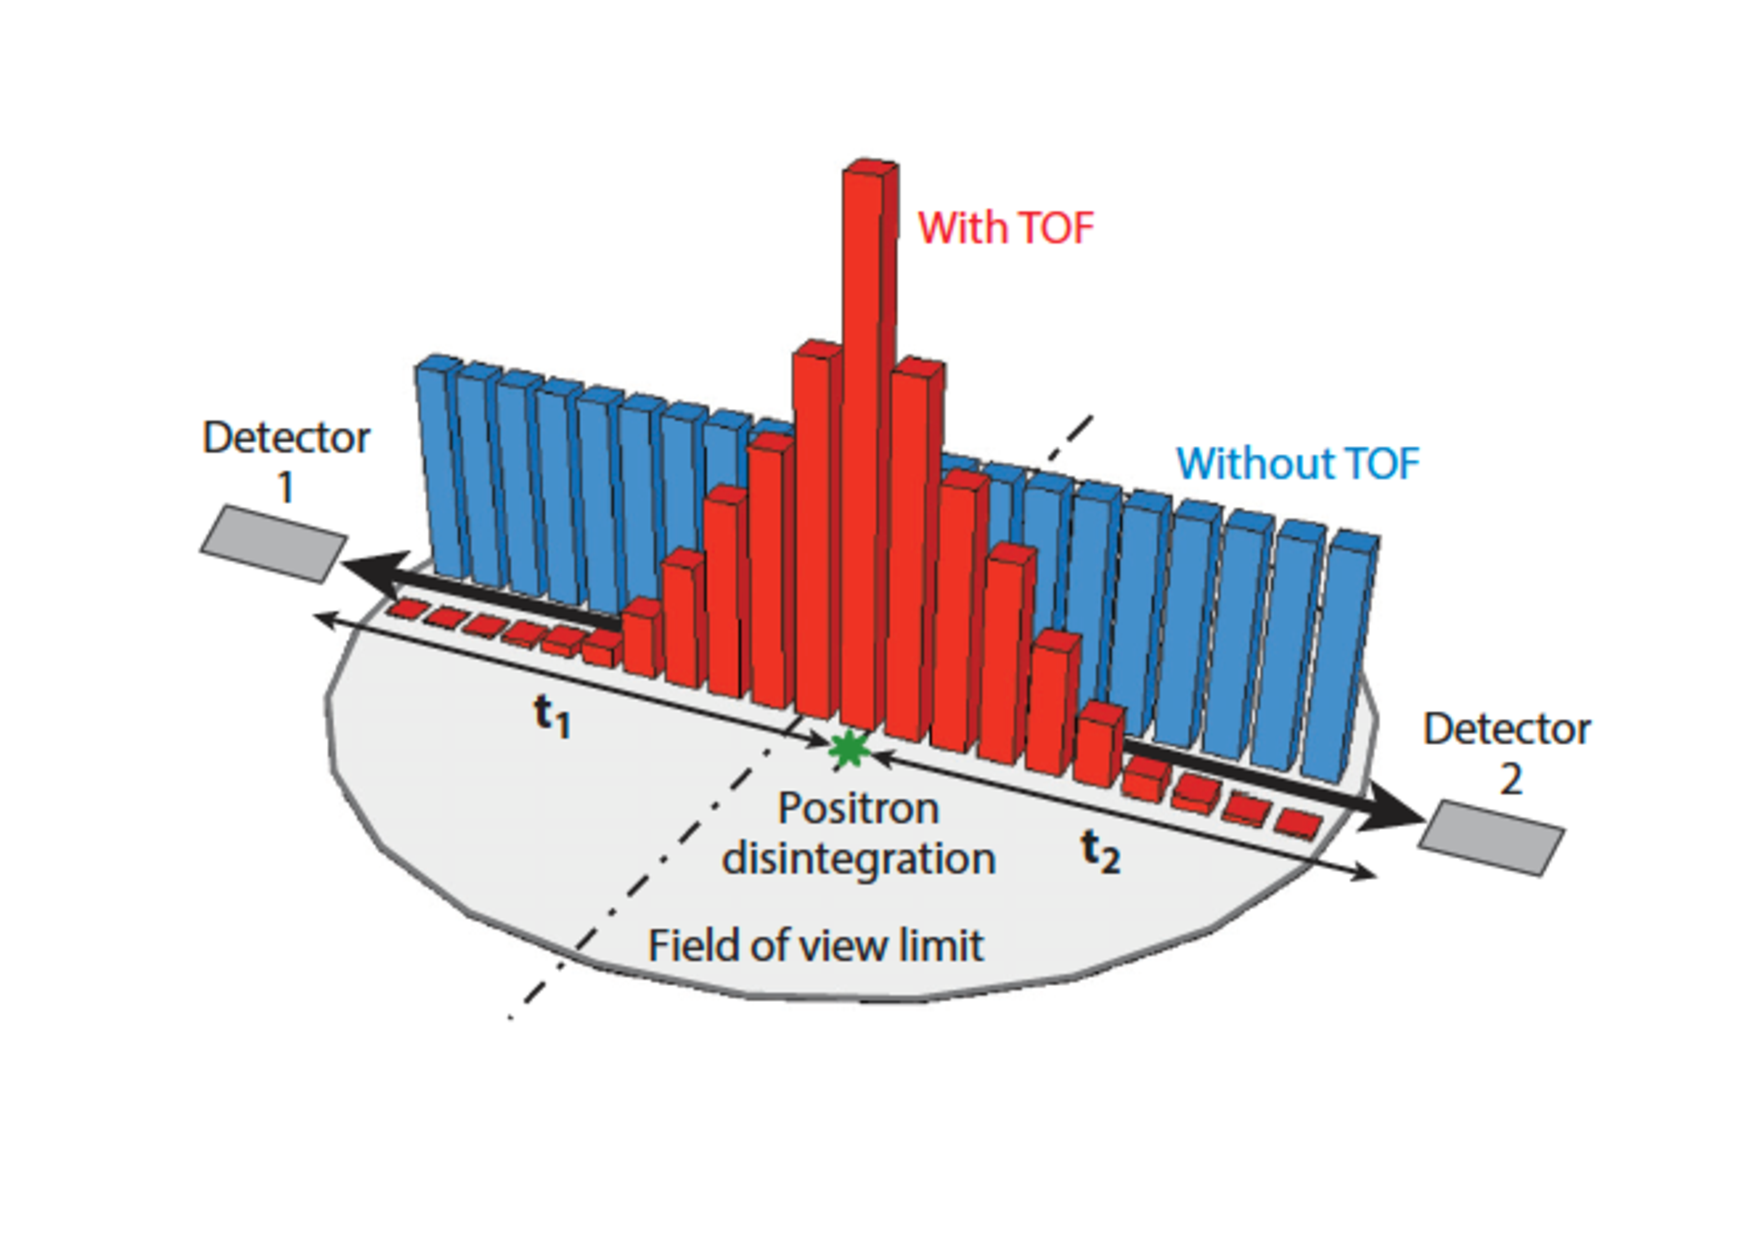
\includegraphics[width=0.8\textwidth]{03_GraphicFiles/chapter1_Introduction/PET_TOF.pdf}
\caption{Schematic view of the information provided by \gls{tof} measurement to the \gls{pet} detection. Without \gls{tof}, a flat probability is assigned to the reconstructed \gls{lor} (blue), while the measurement of the arrival time difference between the two coincident photons is translated into a distance from the \gls{lor} midpoint where the probability density function should centered (red). In~\cite{Vaquero2015}.}
\label{chap1::fig::NM_PET_TOF}
\end{figure}   

This possibility was explored already in the 1980s with fast scintillators~\parencite{Ter-Pogossian1982, Lewellen1988}, such as \gls{csf} and \gls{baf2}, which were anyway not adapted to clinical \gls{pet} application due to a low stopping power. On the other hand, the \gls{bgo} response was too slow to perform \gls{tof}. With the introduction of \gls{lso}, it was also recognized that its very good timing resolution (together with the one of the similar scintillator \gls{lyso}) could be utilized in the development of \gls{tof}-\gls{pet} systems~\parencite{Moses1999}, overcoming the limitation of the early designs of the 1980s. In 2005 Siemens presented the results from a prototype that achieved a timing resolution of 1.2~ns, and soon after the first \gls{tof}-\gls{pet} machine was launched by Philips (Philips Gemini TF)~\parencite{Karp2008}.  Based on \gls{lyso} crystal, it provided 585~ps system timing resolution. At present, all the main \gls{pet} vendors offer \gls{tof}-\gls{pet} solutions with hundreds of ps timing resolution. 
Beyond PET detector designs using conventional \glspl{pm}, the arrival of \glspl{sipm} has led to a great interest in utilizing these new photosensors to achieve improved timing resolution in \gls{tof}-\gls{pet} scanners. Philips recently introduced the Vereos system, which uses digital  \glspl{sipm} for signal readout from individual \gls{lyso} crystals; such a machine provides a system coincidence timing resolution of approximately 310 ps~\parencite{Miller2015}. In parallel \gls{ge} developed the SIGNA \gls{tof}-\gls{pet}/\gls{mri} system using a detector ring based on analog \glspl{sipm} inserted in the magnet bore, thereby
allowing simultaneous \gls{pet} and MR imaging. The reported system coincidence timing resolution of this system is 390–400~ps~\parencite{Levin2013}. Hence, while scanners with detectors using conventional \glspl{pm} are pushing closer to 400~ps timing resolution, new \gls{sipm} technology indicates that system resolution close to 300~ps is achievable with the lutetium based scintillators.
With the rapid improvements of both scintillator and photosensor technology shown by recent results, a \gls{tof} resolution below 100~ps seems achievable in the next future~\parencite{Surti2016, Lecoq2017}.
Recent studies also investigated cost-effective solutions to achieve performance comparable to present commercial systems. In particular, a whole-body \gls{pet} scanner based on plastic scintillators is being developed in Poland by the Jagiellonian University group. The J-PET is constructed with axially arranged strips of plastic scintillators, aiming to detect the annihilation photons via Compton interaction and read out on both sides by \glspl{pm}. The position of interaction in the scintillator is determined from the time difference of light signal arriving on each strip end. A \gls{tot} technique is used instead of the charge measurement of standard \gls{pet} systems in order to take advantage of the superior timing properties of plastic scintillators with respect to crystal detectors (\gls{lso} and \gls{bgo}). Preliminary studies showed that it is possible to achieve a coincidence time resolution of about 500~ps \gls{fwhm} with simple time measurements, coupled to a few millimeters spatial resolution~\parencite{Niedzwiecki2017}.

\subsection{Single Photon Emission Computed Tomography}\label{chap1::subsec::SPECT_NM}
In \gls{spect} tomographic images of the radionuclide distribution in the patient are generated from the emitted gamma photons detected as singles with collimated scintillators. Planar imaging reproduces a two-dimensional projection of the tracer distribution from a single view, while the tomographic image is obtained by the reconstruction of several slices collected from multiple camera positions. Both techniques are used in clinics: planar imaging is less demanding and only requires a single camera head, while multiple camera heads mounted on a rotating gantry are generally used for tomographic imaging, and image reconstruction is required.

Although many innovations have been made since the introduction of the first gamma camera in 1958 by Hal Anger~\parencite{Anger1958}, today's clinical detectors share many of the essential features of Anger's early designs, and are often called Anger cameras. A standard \gls{spect} gamma camera is composed of an aperture or collimator which mechanically selects photons traveling in specific directions, depending on the collimator configuration. The photons approaching the camera from directions different than those specified by the collimation system are passively absorbed. The gamma photons with the selected direction then encounter a scintillation detectors coupled to photosensors. The related electronics and data acquisition system are generally optimized to impose energy threshold in order to reject undesired photons, such the ones which underwent scattering in the collimator section. A schematic view of the main component of the \gls{spect} camera is given in \figurename~\ref{chap1::fig::SPECT_components}, while a simplified view of the collimation principle is sketched in \figurename~\ref{chap1::fig::SPECT_collimator}.   

 \begin{figure}[!htbp]
\begin{subfigure}[t]{.49\textwidth}
\centering
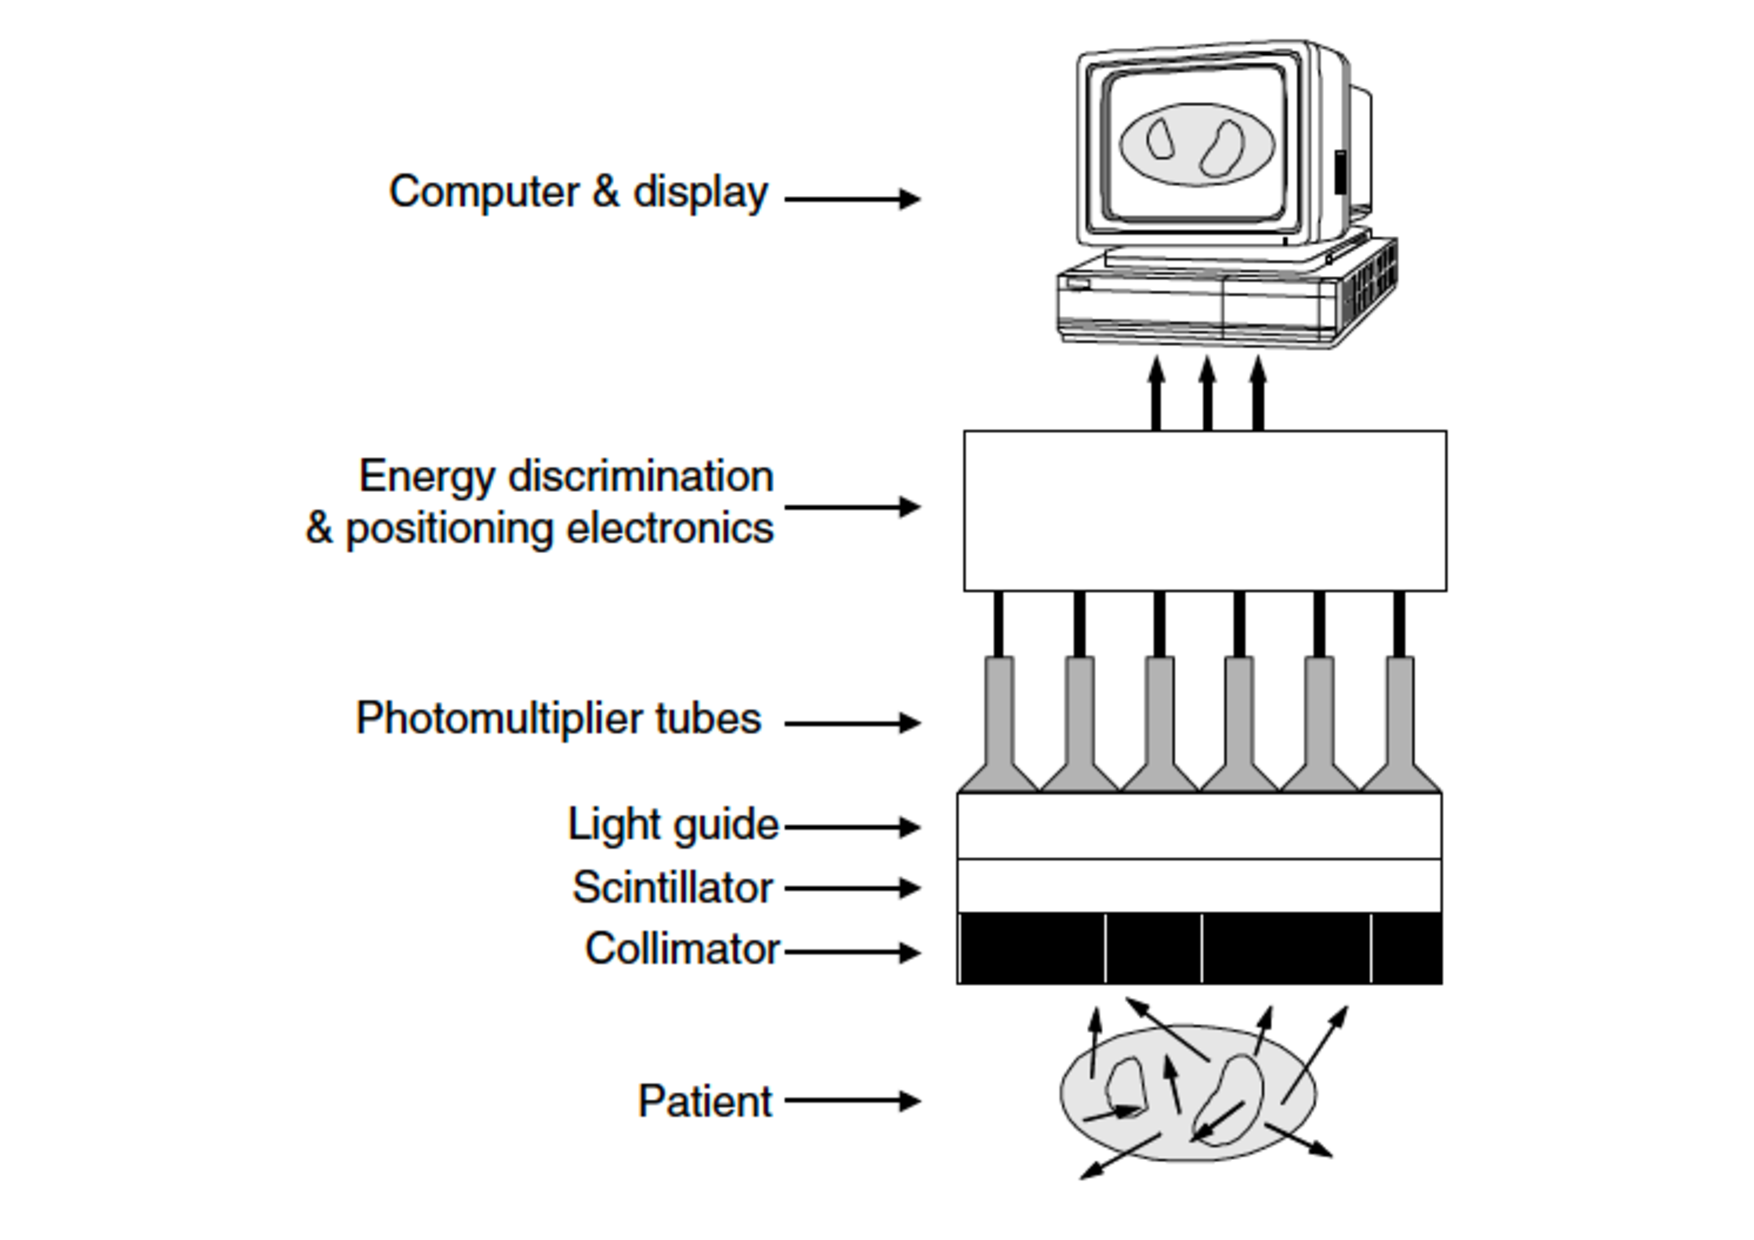
\includegraphics[width=0.7\linewidth]{03_GraphicFiles/chapter1_Introduction/SPECT_components.pdf}
\caption{Schematic view of the main components of a \gls{spect} gamma camera.}
\label{chap1::fig::SPECT_components}
\end{subfigure}
\begin{subfigure}[t]{.49\textwidth}
\centering
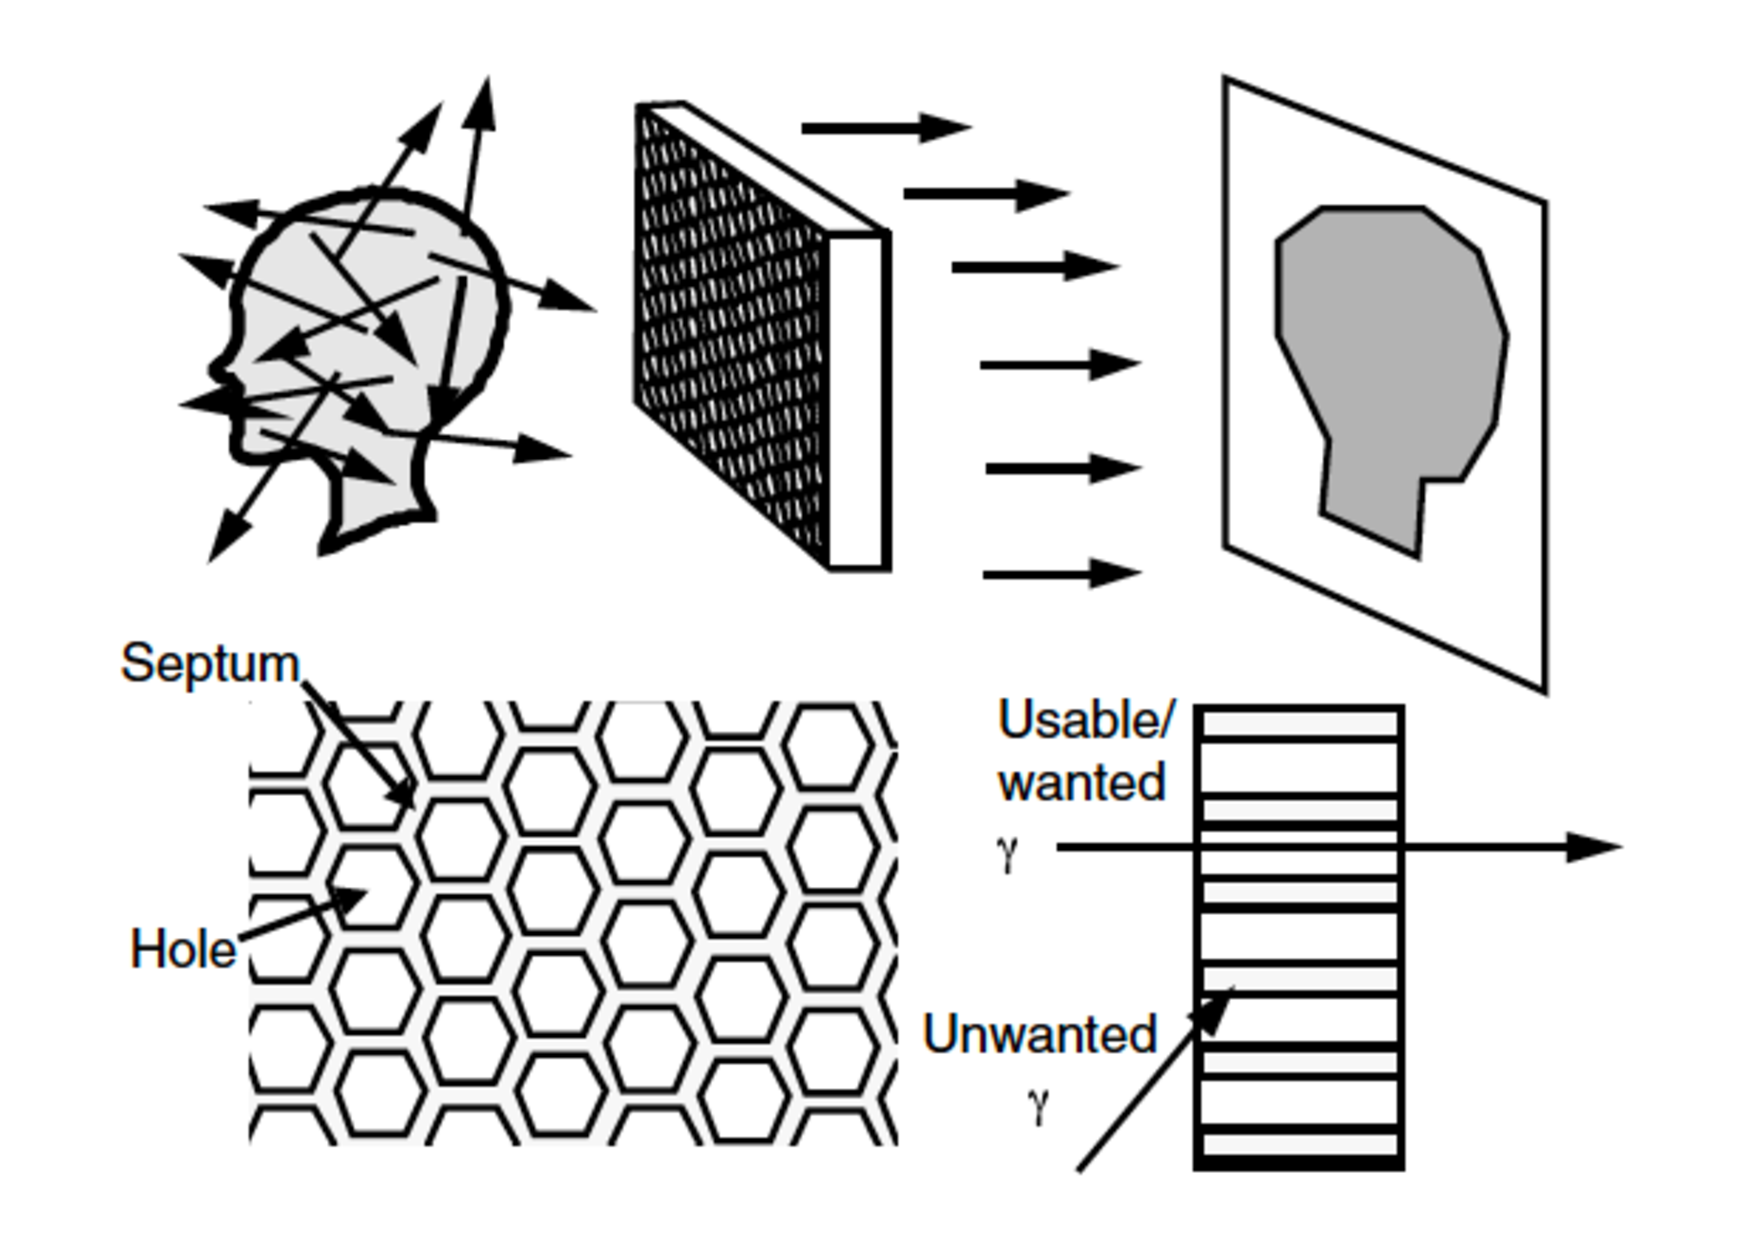
\includegraphics[width=0.98\linewidth]{03_GraphicFiles/chapter1_Introduction/SPECT_collimator.pdf}
\caption{Schematic representation of the collimation principle of \gls{spect} gamma cameras.}
\label{chap1::fig::SPECT_collimator}
\end{subfigure}
\caption{In~\cite{Zeng2004}.}
\label{chap1::fig::SPECT_details}
\end{figure} 

The most simple photon passive selection device is the pinhole aperture, but acceptable spatial resolution can be only obtained at the expense of the system sensitivity. Improved, but always limited overall sensitivity is provided by the introduction of collimators, composed of array of holes separated by septa.  Collimator septa are composed of highly absorbing material with high atomic number and high density. Alloys of lead, tungsten and gold are the most common materials used for this purpose. 
Various hole shapes (circular, square, triangular or hexagonal) are used in common collimators, but the hexagonal shape is the most diffused because it provides the best efficiency. In addition to parallel hole patterns, also converging and diverging collimators have been developed. Converging collimators magnify an image on a camera face and thus can yield finer resolution and/or higher sensitivity images than those resulting from used of parallel-hole collimators. Converging solutions are adapted to small-size objects with respect to the camera \gls{fov}, while the image of large object would result truncated (if part of the object is outside the \gls{fov} of the camera) or distorted (because the magnification is dependent on the distance from the collimator). 
The most spread parallel-hole collimators find routine use in clinics in four configurations: \gls{lehr}, \gls{legp}, \gls{megp}, and \gls{hegp}. Each designation is adapted to a defined gamma energy range, and thus to certain radioisotopes, and is also an indication of the trade-off between resolution and sensitivity which are affected by the septal material, the hole size and length, and the septal thickness. Collimator sensitivity is maximized by the thinnest possible septa, but thin septa can lead to septal penetration which is extremely detrimental to diagnostic performance. The aforementioned trade-off is then a crucial parameter to be considered when designing a \gls{spect} camera, and, together with the employed scintillator and photosensor features, completely determine the overall system performance~\parencite{Gunter2004}.

The origins of \gls{spect} imaging can be identified with the invention of the Anger scintillation camera in the late 1950s~\parencite{Anger1958, Anger1964}; previously, scans were performed by manually positioning a Geiger counter above the organ of interest, but with the Anger camera the entire organ could be scanned at one time. During the 1960s, both longitudinal and transaxial emission tomography were deeply studied. Crandall and Cassen developed a longitudinal tomographic scanner which used a highly focusing collimator placed on a large crystal-matrix detector~\parencite{Crandall1966}, and in 1969, Anger invented a sophisticated longitudinal tomograph that used a scanning scintillation camera~\parencite{Anger1969}. Transaxial tomographs were developed by Kuhl and colleagues between 1963 and 1976, and the final prototype used discrete scintillator arrays~\parencite{Kuhl1976}. Discrete scintillation detectors have been also used for other scanners in the late 1970s, but the first investigators to explore the possible implementation of an Anger camera for transaxial tomography were Paul Harper and colleagues at the University of Chicago. In the early stages, a rotatable chair was placed in fornt of a single head fixed Anger camera~\parencite{Muehllehner1971}. In 1976, Jaszczak and Keyes, independently developed a \gls{spect} system that used an Anger camera mounted on a rotating gantry~\parencite{Jaszczak1977, Keyes1977}. In the following years, the first whole-body \gls{spect} system was developed and clinically evaluated in 1978 at the Baylor College of Medicine~\parencite{Jaszczak1979}. During the late 1970s and the 1980s, both rotating-camera \gls{spect} systems and stationary detector configurations were proposed and developed in Europe and US~\parencite{Larsson1980, Rogers1988}, and the bases for modern machines were established. 
The modern cameras, as mentioned, rely on the described designs and have been adapted.in the past years, to new tracers provided by the pharmaceutical industry. \gls{spect} takes advantage of many years of experience and is now a well-established imaging modality in nuclear medicine. Thanks to its cost-effectiveness, such an imaging technique is widely employed in the clinical routine, and all the major medical imaging companies offer a \gls{spect} system, generally in dual-head configuration with rotating gantry.
At present, virtually all single-photon imaging in nuclear medicine relies on Anger-type cameras, relatively simple and cost-effective, but limited in sensitivity and energy acceptance given the presence of a mechanical photon selection system. Already in 1974 this limitation was addressed by Todd and Nightingale which proposed the application of Compton imaging method to nuclear medicine~\parencite{Todd1974}. The Compton detection principle is described in chapter~\ref{chap::2}. Starting from 1981, Singh and colleagues published a number of seminal papaers that described analytical and experimental results for Compton camera composed of a pixelated germanium first detector and a standard Anger camera as second detector~\parencite{Singh1981, Singh1983, Singh1983b}. The investigation of such an imaging modality for the application in single photon detection for nuclear medicine continued in the following year and is still today actively explored. In particular, the availability of new high-energy tracers could provide advantages in terms of dose and spatial accuracy, but high-energy photons are hardly collimated with mechanical passive system. The electronic collimation exploited by Compton cameras can be the solution for high-sensitivity and high-resolution \gls{spect} examinations. More details can be found in in chapter~\ref{chap::5} of this thesis, where the described topic has been addressed with simulation studies. The presented results have been recently published in~\parencite{Fontana2017_PMB} and~\parencite{Fontana2017_APPB}. 

\subsection{Theranostics}\label{chap1::subsec::Theranostics}

The theranostics approach in nuclear medicine couples diagnostic imaging and cancer therapy using the same molecule or at least very similar drugs, given in different dosages. For example, the combination of \gls{iod131} (gamma emitter) and \gls{lut177} (beta emitter), is used for both imaging and therapy. Furthermore, different isotopes of the same elements (for example \gls{iod123}, \gls{iod131} and the newer terbium isotopes - Tb) can also be used for theranostics given the multiple associated emission (beta and gamma, gamma rays at different energies, alpha and gamma)~\parencite{Gerard2002, Alzahrani2012, Muller2012}. During the treatment, theranostics can be applied in monitoring the therapy course and estimating the potential response and eventual toxicity. The safety of high cumulative doses of radioactive agents after multiple repeated cycles is, however, a cause of concern. Anyway, remarkable improvements have been obtained in targeted therapies, which have proven to be effective with favorable safety profiles~\parencite{Baum2012, Kwekkeboom2008, Strosberg2017}. The diagnostic part of theranostics can be performed with both \gls{pet} and \gls{spect} machines, depending on the employed radioisotope emissions. Most therapeutic radiopharmaceuticals are labeled with $\beta^{-}$-emitting isotopes, having a tissue penetration of only few millimeters and so adapted to spare the healthy tissues surrounding the tumor. The first theranostic radiopharmaceutical in nuclear medicine history was radioiodine, used for therapy and imaging in thyroid diseases~\parencite{Hertz2016}. iodine is taken up by the thyroid galnd for the production of hormones, vital for the development of the brain, normal growth and metabolic balance. In 19367, Hertz developed the idea of administrating radioactive iodine in patients with thyroid diseases, and few years of preclinical studies at the \gls{mit} (where the first cyclotron for medical use had been built) followed this first proposal. In 1941, the first patient was treated with radioiodine~\parencite{Hertz1942}. \gls{iod131} is to the date the gold standard for certain therapeutical indications, given its low cost and the advantageous combination of $\beta^{-}$ and gamma emission. The electron radiation targets the thyroid from the inside, while the organ can be visualized using a gamma camera.  

Since its first proposal, the use of theranostic agents has been consistently increasing: the combination of targeted cancer imaging and therapy is a considerable contribution to personalized medicine and may play an important role in the future with the implementation of new chemical agents and the continuous improvement of imaging systems~\parencite{Yordanova2017}. For the peculiar context of this thesis it is worth to notice that, as for diagnosis \gls{spect}, high-energy gamma emitters can be applied in theranostics, and Compton camera can be implemented for the imaging task. This point is further discussed in chapter~\ref{chap::5}. 


\clearpage
%\printbibliography[heading=subbibintoc]


% Main Part
\chapter{Gamma cameras}\label{chap::2}

\vfill

\minitoc

\newpage


\section{Working principle}

\section{Applications in medicine}

\subsection{Ion beam therapy}

\subsection{Nuclear medicine}

LINE CONE RECONSTRUCTION \parencite{Cree1994}, \parencite{Basko1998}, \parencite{Parra1999}, \parencite{Hirasawa2003}, \parencite{Maxim2009} \\

ITERATIVE RECONSTRUCTION \parencite{Schone2010}, \parencite{Zoglauer2011}, \parencite{Gillam2011}, \parencite{Lojacono2013}, \parencite{Mackin2012}\\

\section{State of the art}

\clearpage
%\printbibliography[heading=subbibintoc]


\chapter{CLaRyS prototypes}\label{chap::3}


\vfill

\minitoc

\newpage

\glsresetall


Following the highlighted limits of ion beam therapy (see chapter~\ref{chap::1}), a collaboration of five French research institutions was established in 2008 (??) with the aim of exploring different experimental solutions for the ion range online monitoring. The research group originally involved the \enquote{\gls{ipnl}}, the \enquote{\gls{cppm}}, the \enquote{\gls{lpsc}} in Grenoble, the \enquote{\gls{lpc}} and the \enquote{\gls{creatis}} in Lyon. The collaboration focuses on the investigation of methods and detection solution for the online monitoring of ion beam range during ion beam therapy treatment, and is so called \gls{clarys}.\\
The main goal of the created collaboration is the parallel development of three gamma detection systems to be employed for ion range online monitoring purpose in the ion beam therapy field: a \gls{pet} detector, a multi-collimated gamma camera and a Compton camera.\\ The design and development of the \gls{pet} system is mainly managed by the \gls{lpc} group, which left the collaboration in 2017, and the this detection system is not treated in this thesis work.\\ 
In this chapter the two gamma cameras (multi-collimated and Compton) prototypes are described in details, and the present status of the instrumental development is presented. In the following, an entire chapter (chapter~\ref{chap::6}) is dedicated to the tests of the detectors performed on ion beams. 

\section{CLaRyS gamma camera components}\label{chap3::sec::CLaRyScameras}

The two gamma cameras under development by the CLaRyS collaboration are devoted to the detection of prompt-gamma rays emitted during ion beam treatments (see section~\ref{chap1::sec::PromptGammas}). The design of the two cameras has been optimized by different Monte Carlo simulation studies for what concerns both the detector components and the geometrical setup.\\
As already mentioned, a Compton camera is usually composed of two detector sections, a scatterer and an absorber: the CLaRyS prototype respects the standard design. In the scatterer, described in section~\ref{chap3::subsec::scatterer}, the prompt-gamma incoming ray is deflected by Compton interaction and the interaction position and energy deposited are stored. The scattered photon reaches then the absorber section, where its energy is ideally totally deposited and stored, again with the interaction position. This configuration is used to provide what is usually defined as \enquote{electronic collimation}, but a mechanical collimation is still an option for photon detection and localization. The scatterer section can be replaced by a mechanical collimator, described in section~\ref{chap3::subsec::collimator}, which selects the parallel incoming photons then absorbed by the same absorber detector (a geometrical setup adaptation is possible to optimize the detection performance and will be discussed in the following). The mechanically collimated system is called multi-collimated camera, due to the collimator multi-slit structure.\\ 
As underlined in section~\ref{chap1::sec::background}, the prompt-gamma measurements are affected by several sources of background: in particular, the signals detected by the two cameras can come from secondary particles other then prompt-gammas, like photons from positron annihilation, neutrons and protons (for beam of ions heavier then protons). One of the possible solution for background rejection is the use of \gls{tof} information (see section~\ref{chap1::sec::TOF}), requiring a further detection section dedicated to the beam tagging. A beam tagging hodoscope is being developed in parallel and can be coupled to both the gamma cameras for \gls{tof} measurements; its description is presented in section~\ref{chap3::subsec::hodoscope}.\\
A schematic view of the two prototypes is given in figure~\ref{chap3::fig::camerasScheme}.\\

\begin{figure}
\begin{subfigure}[b]{.5\textwidth}
\centering
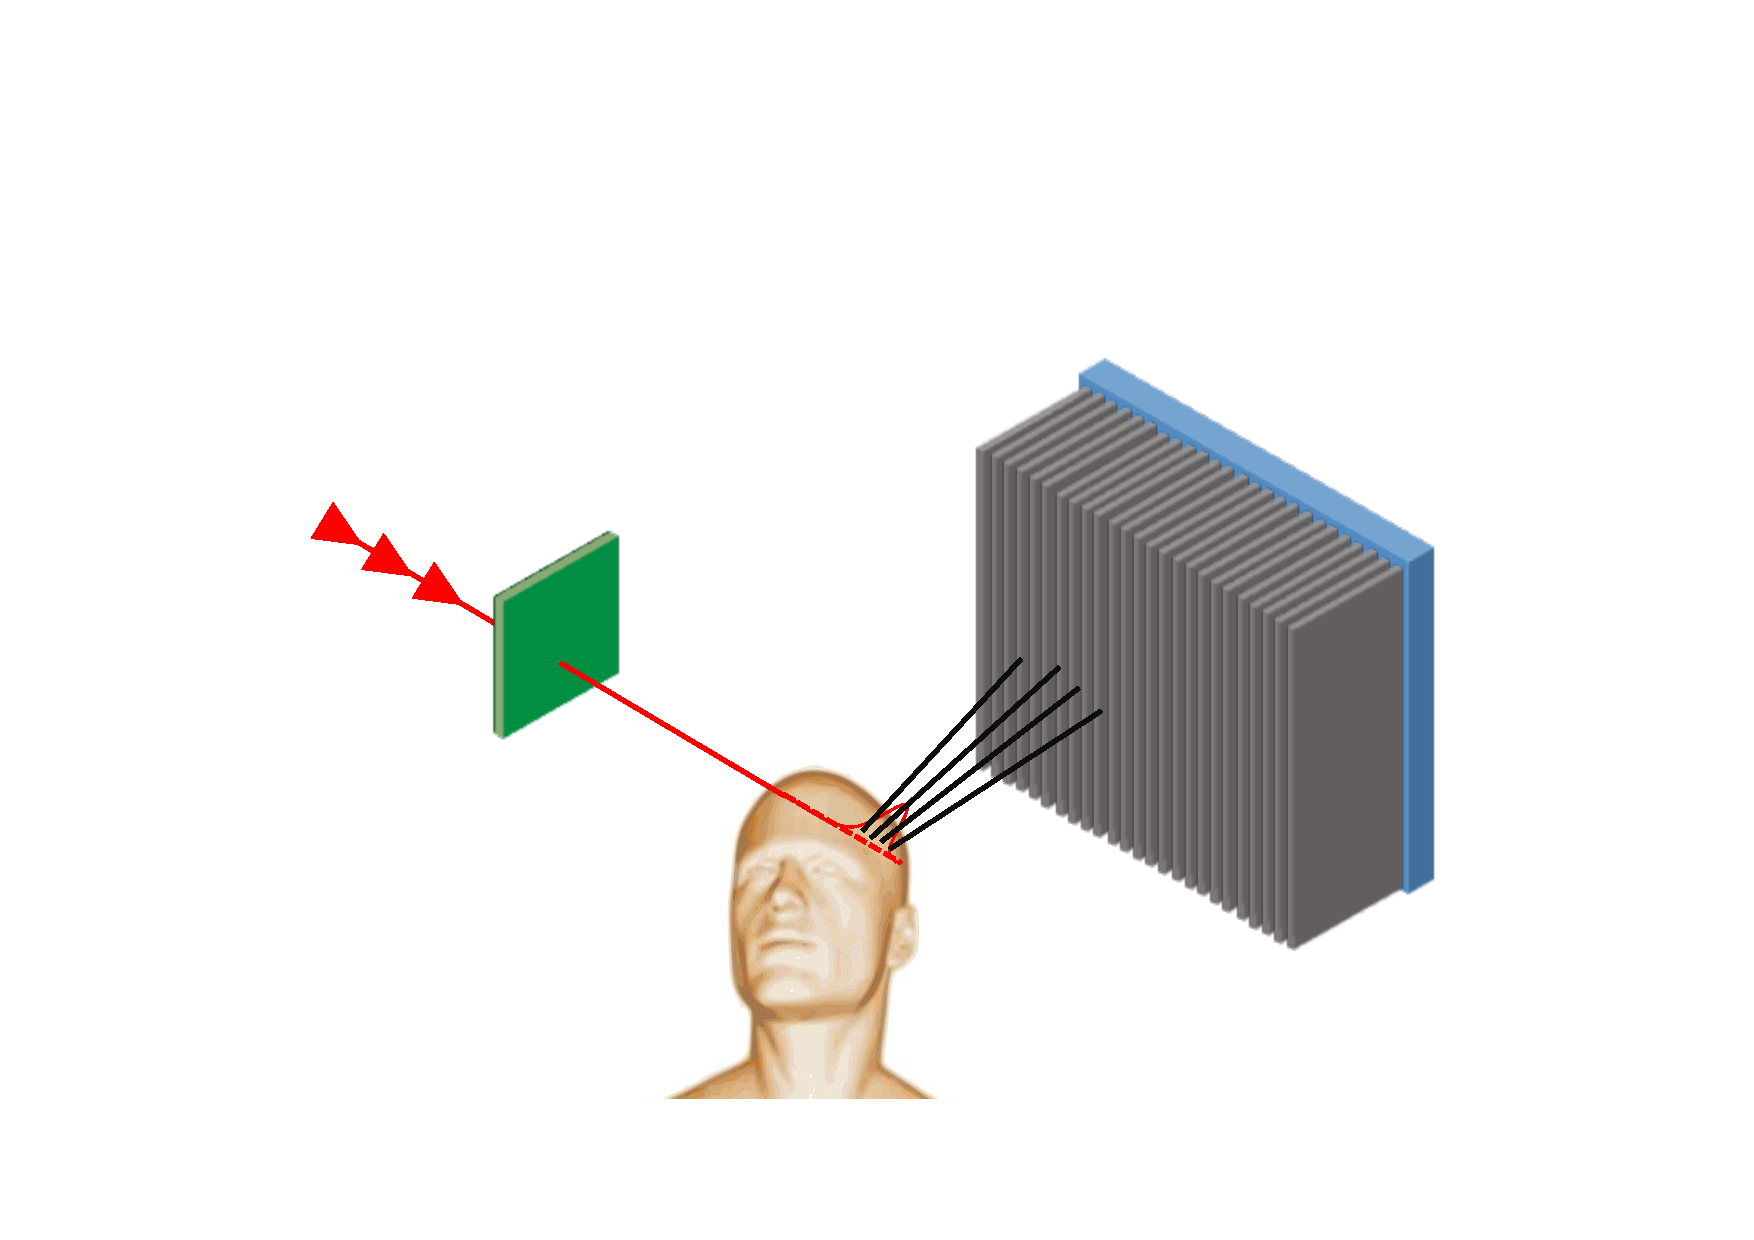
\includegraphics[width=1.2\textwidth]{03_GraphicFiles/chapter3_CLaRySproto/schemes/schema_Collimated_withHodo.pdf}
\caption{Scheme of the multi-collimated camera with the beam tagging hodoscope.}
\label{chap3::subfig::multiCollScheme}
\end{subfigure}
\begin{subfigure}[b]{.5\textwidth}
\centering
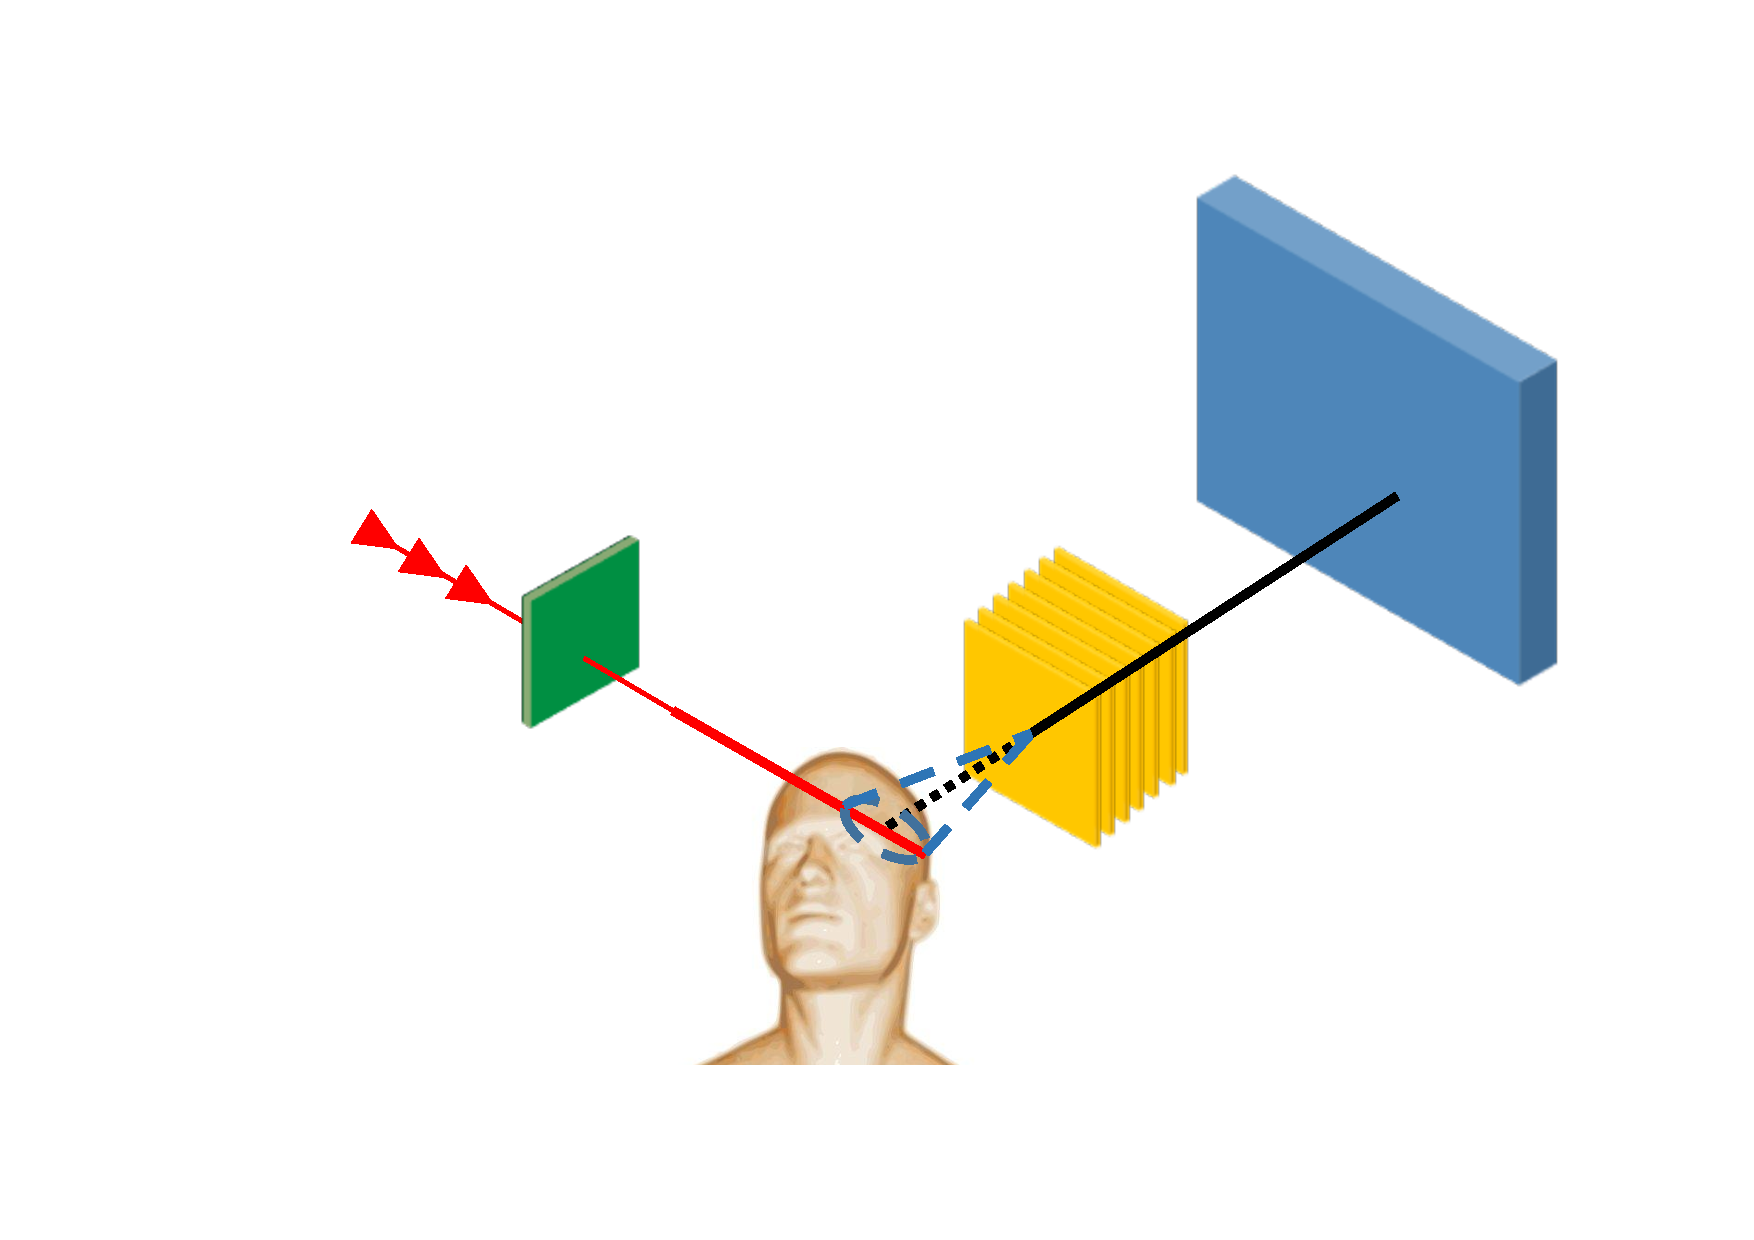
\includegraphics[width=1.2\textwidth]{03_GraphicFiles/chapter3_CLaRySproto/schemes/schema_Compton_withHodo.pdf}	
\caption{Scheme of the Compton camera with the beam tagging hodoscope.}
\label{chap3::subfig::ComptonScheme}
\end{subfigure}
\caption{Schematic view of the two CLaRyS gamma camera prototypes: the multi-collimated camera (top) and the Compton camera (bottom).}
\label{chap3::fig::camerasScheme}
\end{figure}
 

%%%%%%%%%%%%%%%%%%%%%%%%%%%%%%%%%%   SCATTERER  %%%%%%%%%%%%%%%%%%%%%%%%%%%%%%%%%%%%%%%%%%%%

\subsection{Scatterer}\label{chap3::subsec::scatterer} 
The scatterer stack is one of the components of the Compton camera prototype. Dedicated to the photon Compton scattering, its design has been studied to fulfill the camera requirements.\\ 
The Compton events reconstruction strongly relies on the measurement of the energy deposited by the photon in its Compton interaction, mandatory to properly calculate the Compton scattering angle, which is then the aperture of the resulting Compton cone. The camera accuracy is then strictly dependent on the scatterer energy resolution. At the same time, the camera efficiency is dominated by the balance between Compton interaction and photoelectric absorption probability in the scatterer detector.\\
Given the need of at least two interactions for a proper event reconstruction (a Compton scattering in the scatterer section and an ideally complete absorption in the absorber section, described in~\ref{chap3::subsec::absorber}), the material choice and the geometrical configuration play a fundamental role in the camera operation. The setup must be tuned in order to define the better trade-off between Compton and photoelectric interaction probability and to optimize, as mentioned, the detector energy resolution.\\
Given the fact that the Compton interaction probability linearly increases with the material atomic number (Z), while the photoelectric absorption depends on Z$^{n}$ with n varying between 4 and 5 according to the photon primary energy~\parencite{Knoll2000}, it is clear that a low Z material is preferred. Considering now the detector energy resolution, it must be noticed that the main parameter affecting the deposited energy detection is the so called \enquote{Doppler spread}. The Compton angle reconstruction formula in equation~\ref{chap1::eq::Compton} neglects the initial recoil electron state, which is considered free or unbound. The Compton energy transfer continuum results affected by the binding energy of the electron, with a relatively increasing effects for decreasing incident photon energy. This effect adds uncertainty on the reconstructed deposited energy, and so in the Compton angle calculation. Given its direct dependence on the recoil electron binding energy, the \enquote{Doppler spread} is reduced for low Z materials. Following the described theoretical considerations, silicon detectors are the most coherent choice. This choice has been verified in simulation, where a silicon scatterer has been compared to competitor materials; the result are included in the Monte Carlo study presented in chapter~\ref{chap::5}.\\
Dedicated Monte Carlo simulation studies have been performed in order to define the most suitable geometrical configuration for the Compton camera, including the scatterer stack~\parencite{Richard2012}. As a trade-off between detection efficiency and total cost, 10 layers were included in the original scatterer design. Concerning the layer size, about 10$\times$10~cm$^{2}$ of active area in the transverse plane have been identified as the most convenient choice, also considering the absorber size (see section~\ref{chap3::subsec::absorber}) and the distances between the detection sections required by the \gls{tof} measurements and imposed by the detector rate acceptance in clinical conditions (see appendix~\ref{chap::appA}). Moving to the layer thickness, its choice is governed by the definition of the camera operation. The \gls{clarys} Compton camera does not aim to track the Compton recoil electron, which must be then absorbed inside the same scatterer layer where the Compton interaction took place. This requirement is necessary to well reconstruct the Compton interaction angle, which needs the whole transferred energy as parameter; in addition to this, a recoil electron escaping the involved detection layer can interact in a different layer causing false coincidences which affect the camera efficiency and imaging accuracy. In order to minimize the recoil electron escape probability, relatively thick detectors are needed.\\
The technological choice of the collaboration was oriented to silicon \glspl{dssd}, provided by the Norwegian company SINTEF. A schematic view of the detector principle is given in figure~\ref{chap3::fig::dssdTHEO}. The silicon crystal is doped with negative (n) and positive (p) charge carriers on the two opposite sides, creating diodes which are then reverse biased. A polarization voltage is applied to the two opposite sides of the crystal, and a depletion region with no free charges is created. A ionizing particle interacting in the depletion region generates electron-hole pairs in number proportional to the deposited energy. The generated charges drift towards anode (electrons) and cathode (holes) and are converted into electrical signals. The read-out is ensured by the implanted strips, which transfer the charges outside the detection region.\\     

\begin{figure}
\begin{subfigure}[t]{.5\textwidth}
\centering
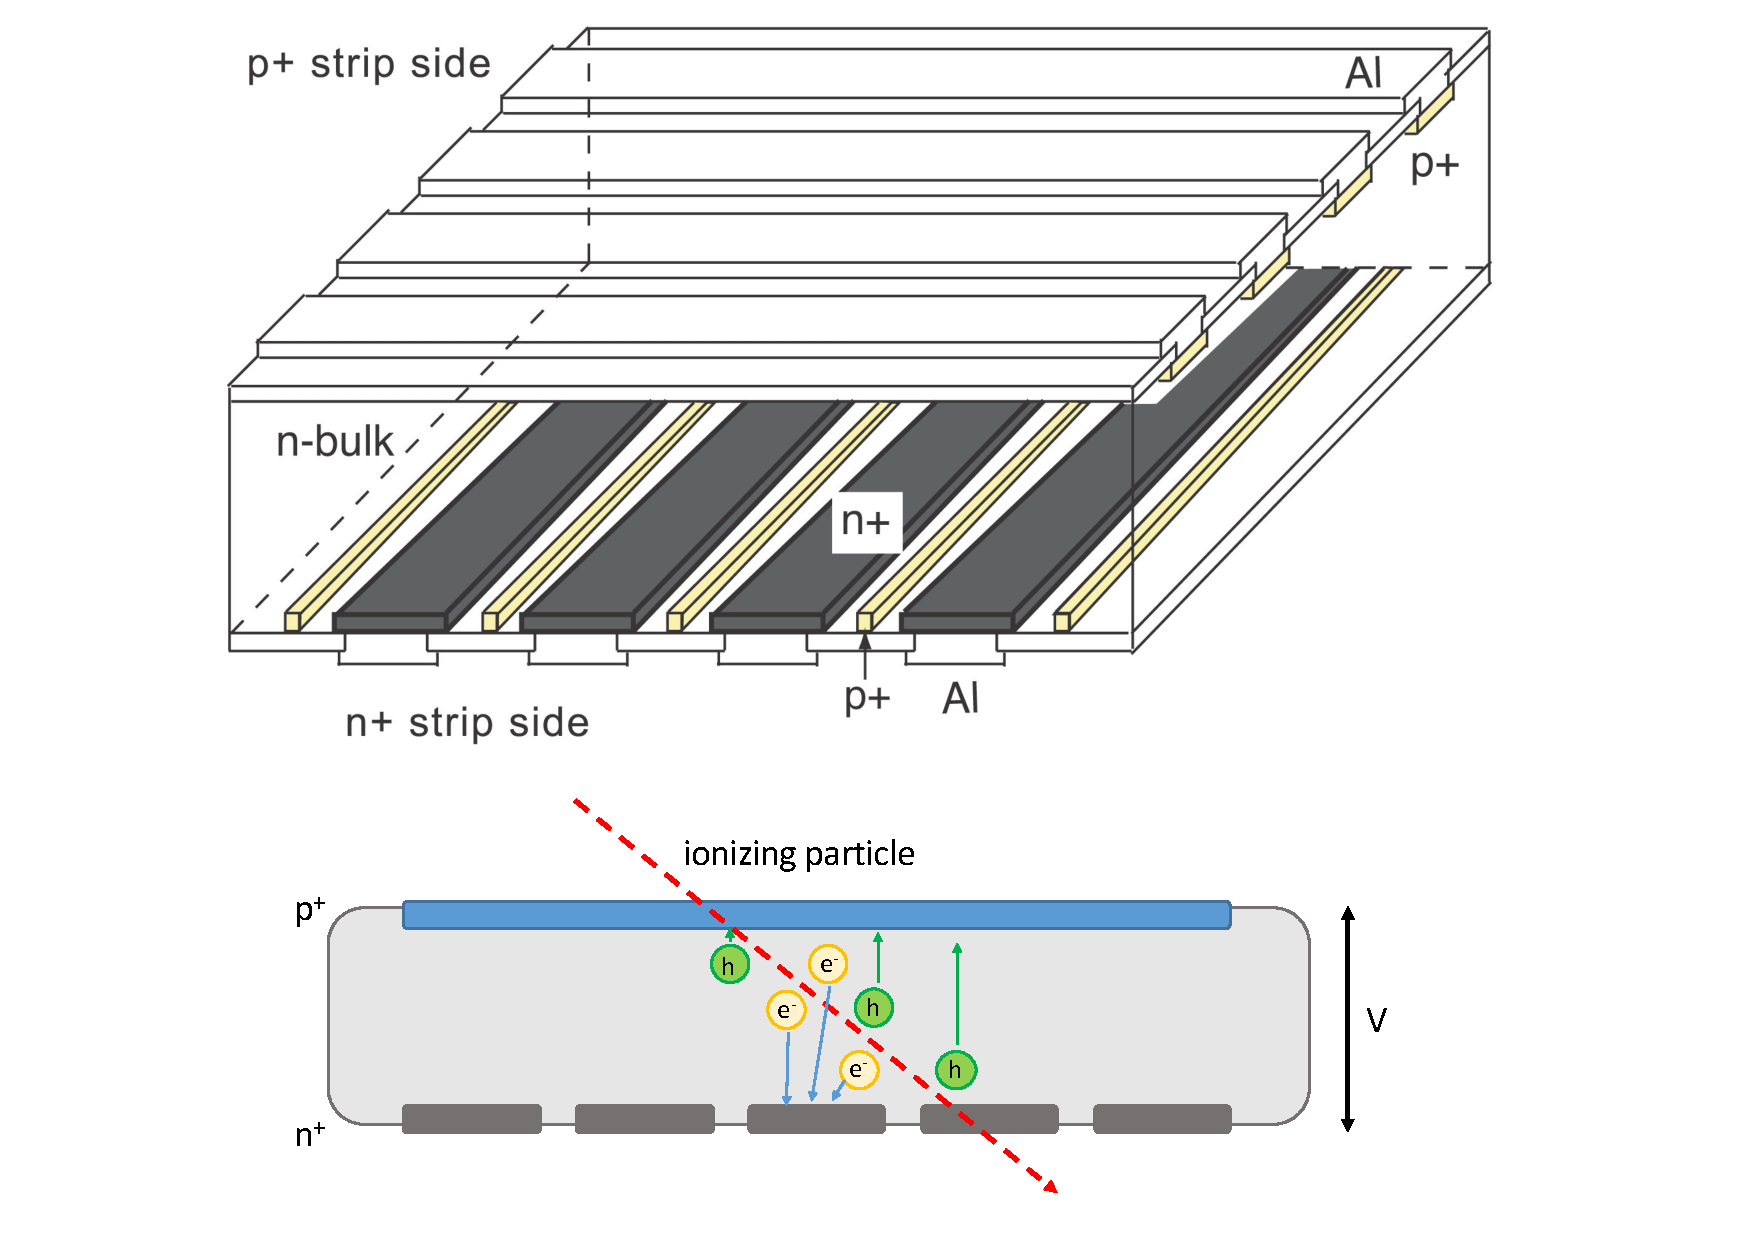
\includegraphics[width=1\textwidth]{03_GraphicFiles/chapter3_CLaRySproto/Scatterer/DSSD_theory_1.pdf}
\caption{Schematic view of a standard \gls{dssd} (from~\cite{Takeda2008}) and sketch of the signal generation.}
\label{chap3::fig::dssdTHEO}
\end{subfigure}
\begin{subfigure}[t]{.5\textwidth}
\centering
\includegraphics[width=1\textwidth, height=16em]{03_GraphicFiles/chapter3_CLaRySproto/Scatterer/ScattererThermalBox.JPG}
\caption{Scatterer silicon layer with its \gls{fe} card in the thermal regulated box (described in section~\ref{chap3::subsubsec::ScattThermBox}).}
\label{chap3::fig::ScattPicture}
\end{subfigure}
\caption{}
\label{chap3::fig::scatterer}
\end{figure} 

Each layer has an active volume of 96$\times$96$\times$2~mm$^{3}$, segmented with 64 strips per detection plane. The strip pitch is 1.41~mm, for a strip width of 1.31~mm. The applied polarization voltage is nominally -750~V, and it is uniformly shared on the whole surface to obtain a homogeneous depletion region. A guard ring, composed of 23 strips surrounding the read-out ones on the p side, ensures the desired voltage gradient. The more peripheral strip of the guard ring is connected to the high voltage, while the n side has a single strip for the guard ring, connected to the ground. The p and n read-out strips are then connected to the \gls{fe} electronics via bonding cables.\\
The \gls{fe} electronics card has been developed by the \gls{ipnl} electronics group and is described in details in section~\ref{chap3::subsubsec::ScattFEcard}. The silicon detector is directly plugged on the card, and the mechanical support for the scatterer stack has been studied according to the card size, as shown in figure~\ref{chap3::fig::ScattPicture}.\\   
Among the 10 received \glspl{dssd}, only 7 fulfilled the requirements imposed by the Compton camera application, mainly in terms of noise level (leakage current); 3 layer have been rejected, so that the final prototype scatterer is composed of 7 silicon planes.\\
The 7 selected layers have been characterized with a temporary acquisition system in terms of leakage current at different temperatures. The results of these measurements can be found in~\cite{Ley2015}. The measurements allowed to verify the producer specifications in terms of polarization voltage to be applied for a complete detector depletion, as well as to identify the noisy strips and create a complete characterization database. In addition to this, they highlighted the need to cool the detectors down with respect to the room temperature (25\textdegree{}C) in order to reduce the leakage current to acceptable levels, and so reducing the total noise level, affecting the detector performance. In order to accomplish the cooling task and respect, at the same time, the clinical restrictions, a thermal regulated box based on cold air pump has been designed and produced. It operates as the scatterer stack mechanical support, and it is described in section~\ref{chap3::subsubsec::ScattThermBox}.\\
      
 

\subsubsection{Scatterer Front-End card}\label{chap3::subsubsec::ScattFEcard}
As mentioned in the previous paragraph, the main requirement for the scatterer detector modules is a very good energy resolution. The desired working performance can be quantified as follows:
\begin{itemize}
\item 1~keV \gls{fwhm} energy resolution;
\item 1.41~mm spatial resolution (corresponding to the strip pitch);
\item 15~ns \gls{fwhm} time resolution.
\end{itemize} 

The scatterer \gls{fe} card has been developed by the \gls{ipnl} electronics group in order to achieve this performance. It is composed of two well separated sections, analog and digital, which must be kept separated in the card layout in order to minimize the contribution of the digital noise on the treatment of the analog signals. Moreover, in order to reduce the electronic noise, the analog section must be placed as close as possible to the detector, to minimize the signal path length.\\
At first, a dedicated \gls{asic} has been designed and developed to treat the signals directly coming from the \gls{dssd}~\parencite{Dahoumane2014}. Each \gls{asic} 
processes 8 detectors channels, so that 8 \gls{asic} per plane are required for the read-out of a complete silicon layer. This section represents the core of the analog stage. The \gls{asic} has been designed and tested to achieve the desired performance in terms of \gls{enc}, which must be lower than 118 electrons \gls{rms} in order to obtain the 1~keV \gls{fwhm} energy resolution, signal dynamics and accepted detection rate. The analog raw signal first passes through a \gls{csa}, which returns an analog amplified signal. This pulse can be further amplified with a \gls{shs} based on a \gls{cr-rc} filter, which filters and shapes the signal in about 1~\charmus, or via a fast amplifier (with 15~ns shaping time). The first mode is used for a refined charge (deposited energy) measurement and can be employed for detector tests and characterization, while the second is the standard working one which allows for fast energy and time measurements. The amplified signal finally passes through a discriminator, which gives a digital output. Analog (from \gls{csa} or \gls{shs}) and digital signals are then sent to the digital stage of the card for the measurement of time, position and energy. To be noticed \\
The digital stage is mainly composed of one \gls{adc} module per \gls{asic} and two \glspl{fpga}. The analog signal from the \gls{asic} is processed by the \gls{adc}, which is a 12-bit module with 8 channels, with a sampling rate of 100~mpsp (Mega Samples Per Second). Each \gls{adc} returns 16 \gls{lvds} pairs (2 per channel), which are sent to the \glspl{fpga} together with two clock signals (two \gls{lvds} pairs) and the 8 digital outputs of the \gls{asic}. So, 44 input channels of the \gls{fpga} are used for the acquisition of 8 read-out channels (one \gls{asic}). Two \glspl{fpga} Altera Cyclone III~\parencite{Altera2012} are installed on the card to handle the signals coming from the whole detector (128 channels, 64 per detection plane): both of them are equipped with a \gls{tdc} for the time measurement.\\
A third \gls{fpga} (Altera StratixII GX~\parencite{Altera2009}) is finally installed on the card to handle the processed data collection and the communication with the acquisition system, described in section~\ref{chap3::subsec::cameraElectronicsDAQ}, via a 3~Gbit/s link.\\
The \gls{asic} has been developed in three versions, and the cards have been optimized during the development process and produced in its final version (shown in figure~\ref{chap3::fig::scattDAQcard}) in the spring 2017. The 7 cards are now available and the development of the \gls{fpga} firmware is ongoing.\\
More details about the card layout, components and operating principle, as well as a description of the tests performed during the development can be found in~\cite{Chen2017} and~\cite{Dahoumane2012}.    

\subsubsection{Scatterer thermal regulated box}\label{chap3::subsubsec::ScattThermBox}

The results of the leakage current tests performed on the silicon detectors showed the need of cooling the detector down to achieve the required performance in terms of noise, which affects the spatial, time and energy resolutions. The leakage current has been studied in temperature cycles in the range -40 - +40~\textdegree{}C, and an overall consistent behavior has been observed both on N and P strips of the detector. The leakage current slightly increases in the range -40 - 0~\textdegree{}C, with values in the range 0 - 8~nA for the analyzed strips, and then drastically increases beyond 0~\textdegree{}C, with peaks of more then 80~nA at +40~\textdegree{}C. The complete description of the performed measurements and the detailed results can be found in~\cite{Ley2015}.\\
A cooling system is needed for the silicon detectors operations: it must be able to keep the temperature constant and below, at least, 0~\textdegree{}C, preferably around -20~\textdegree{}C where the leakage current is more stable in case of small temperature variations. The clinical environment limitations must be considered to design such a cooling system (portability, gas, noise level), as well as the material budget and the mechanical integration with the other camera components.\\
The implemented solution consists in the thermal regulated box shown in figure~\ref{chap3::fig::ScattPicture}, together with one of the silicon layers. The size of the box is 490$\times$490$\times$300~mm$^3$, and the structure is composed of 2~mm of aluminum and three insulation layers of 10~mm of silica aerogel Spaceloft\textsuperscript{\textregistered}~\parencite{Spaceloft2011}, for an equivalent thickness of 2~mm of silicon (0.7\% of interaction probability for 1~MeV photons). The cooling is performed via an electric air pump, which is able to keep the temperature inside the box at -20~\textdegree{}C with a 400~W haet evacuation power. The heat power produced by the 7 silicon \gls{fe} cards in operation must be verified, but the estimate confirms the effectiveness of the thermal box nominal performance. Once card and detector will be fully operational, a test will be performed to check the temperature stability inside the box.\\
The 	\gls{fe} cards and the silicon layers are fixed inside the box via a mechanical support designed and produced by the \gls{ipnl} mechanics group. The support, which ensures a millimeter position accuracy, is fixed on metal rails which allow to easily handle each detector layer. A scheme of the thermal box and the internal support is shown in figure~\ref{chap3::fig::thermalBox}.
    
\begin{figure}
\begin{subfigure}[t]{.5\textwidth}
\centering
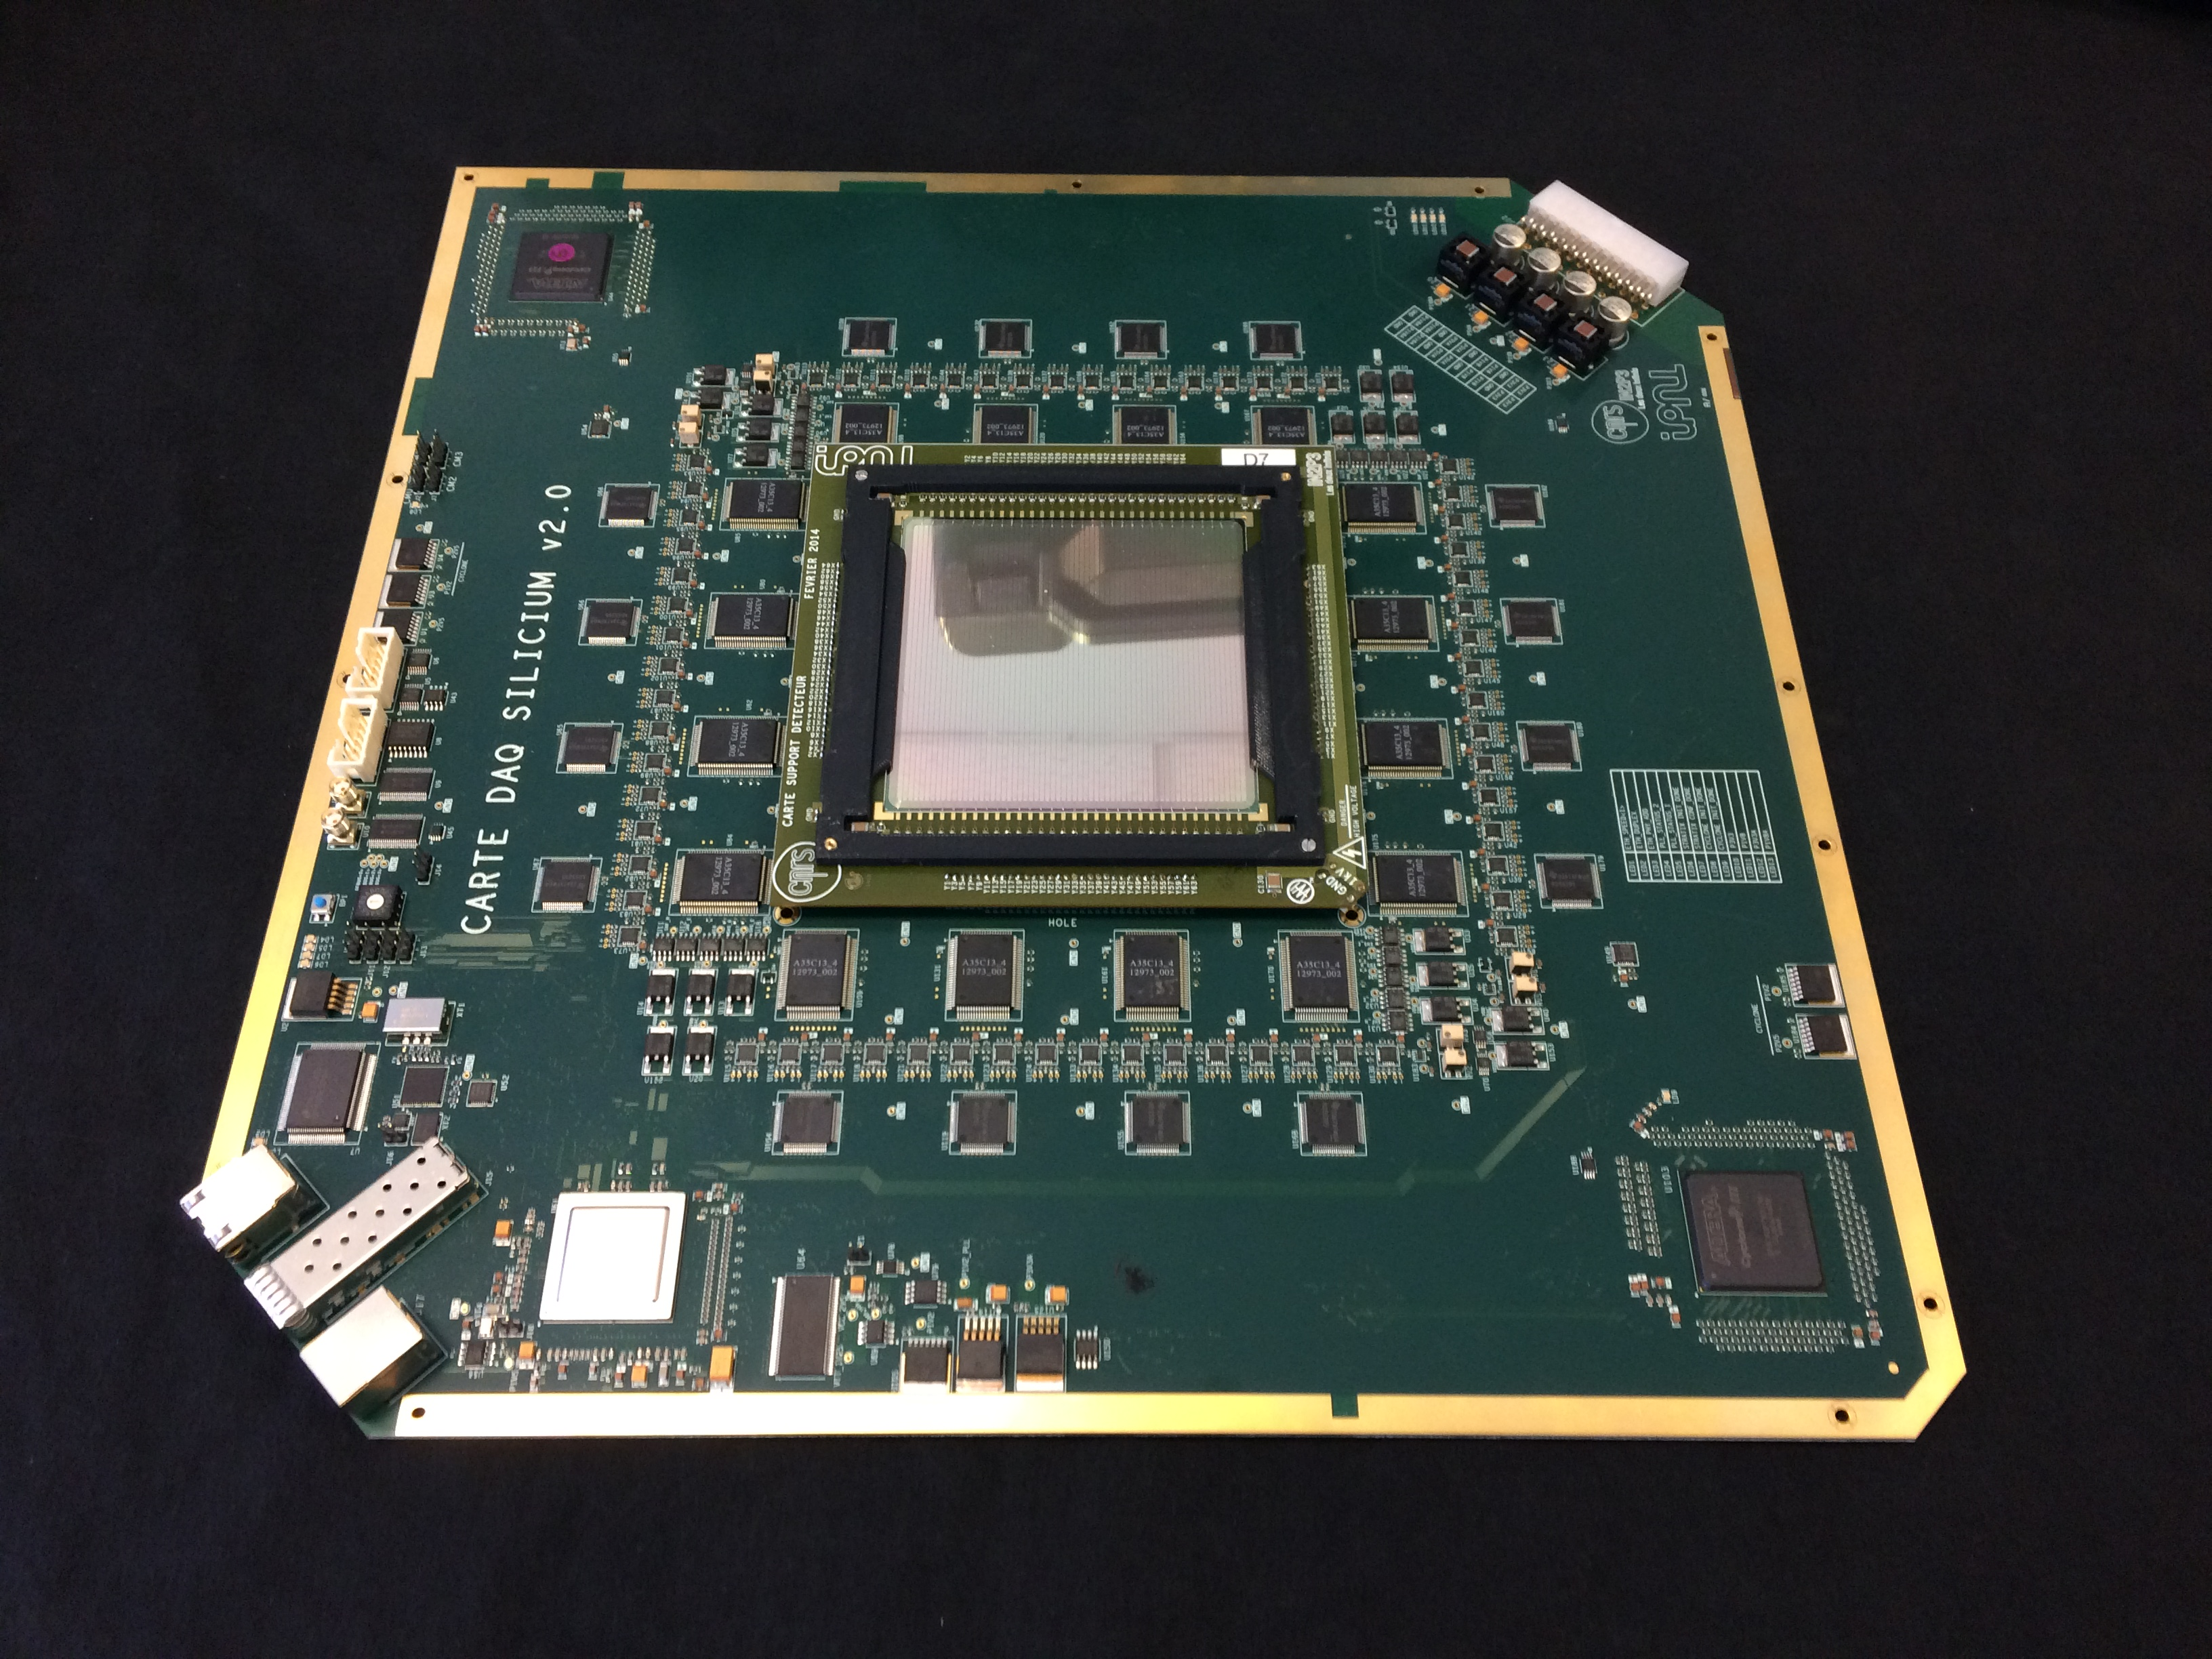
\includegraphics[width=1\textwidth, height = 5.7cm]{03_GraphicFiles/chapter3_CLaRySproto/Scatterer/DAQ_card.JPG}
\caption{Final version of the scatterer \gls{fe} card with the silicon detector layer.}
\label{chap3::fig::scattDAQcard}
\end{subfigure}
\begin{subfigure}[t]{.5\textwidth}
\centering
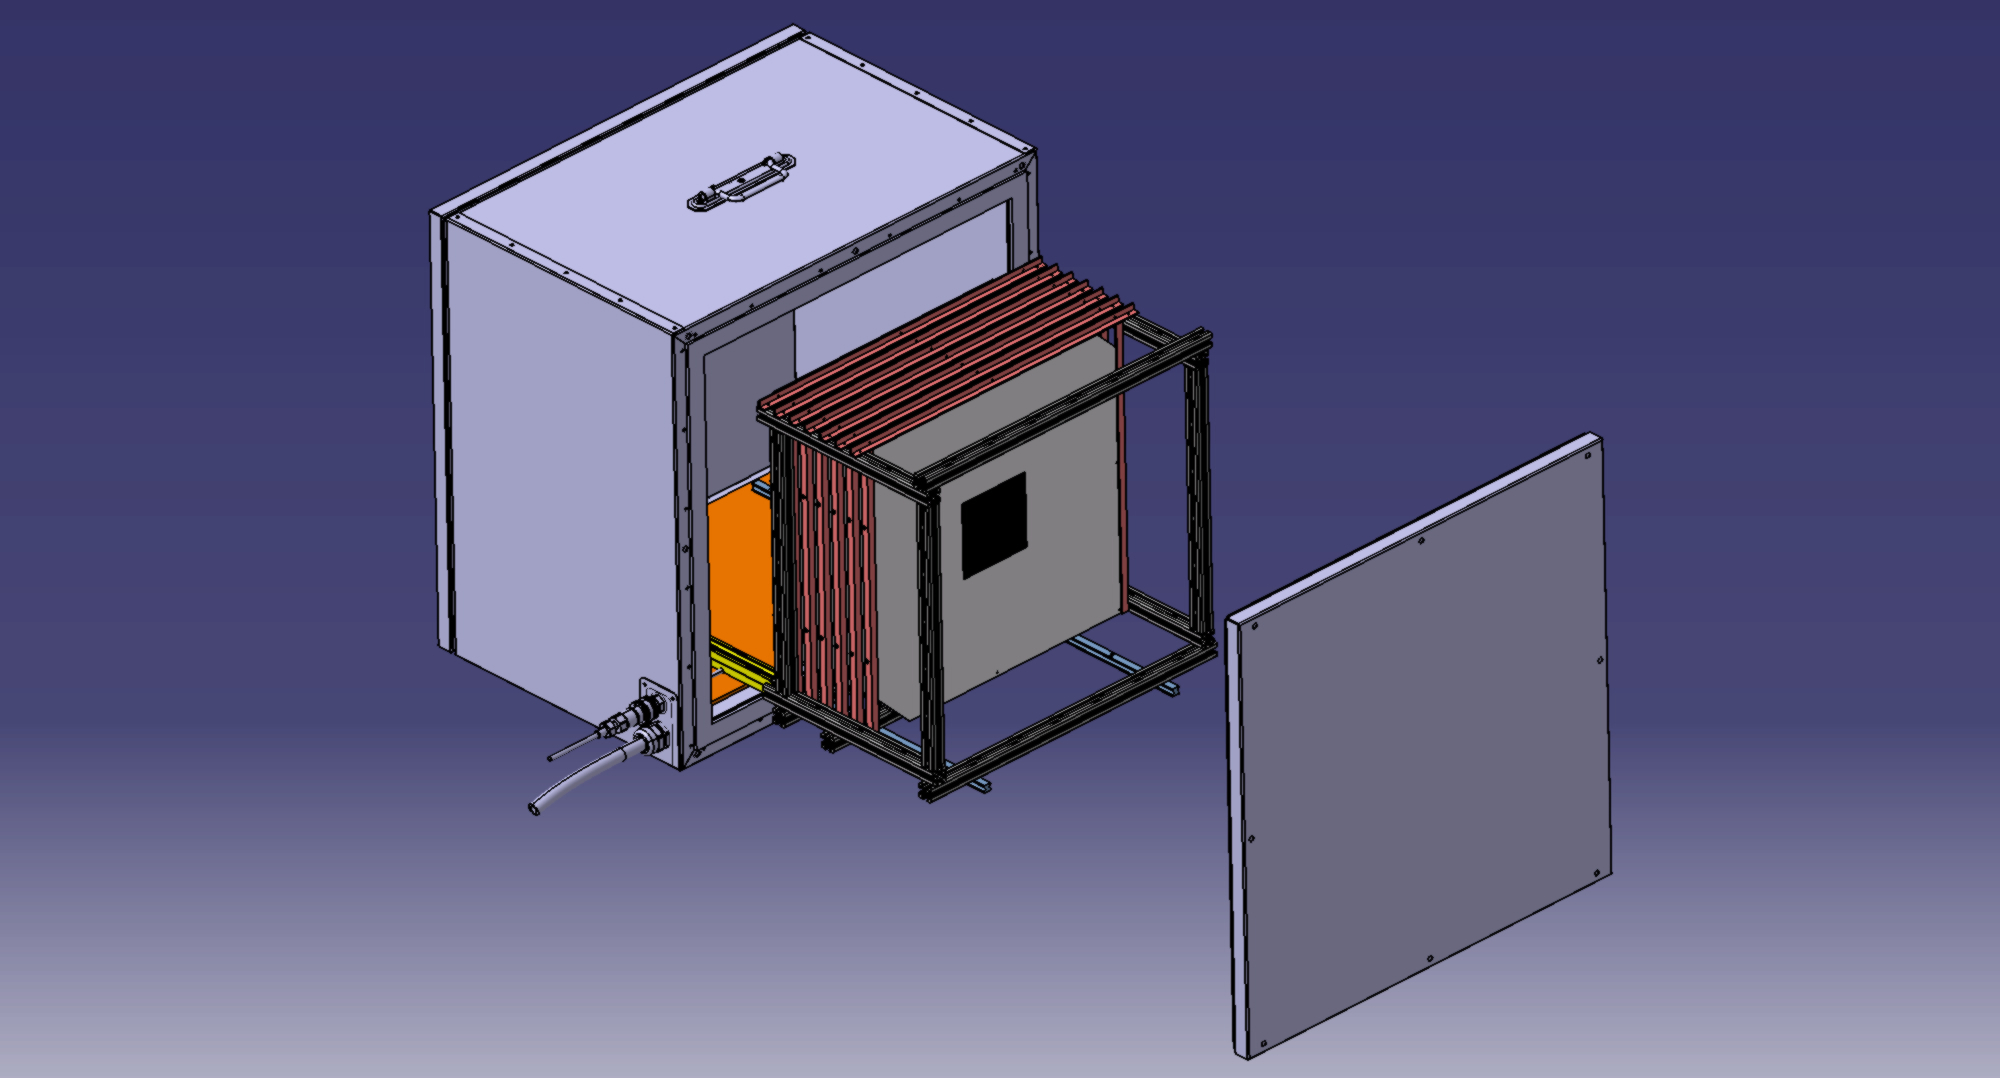
\includegraphics[width=1\textwidth, trim={5cm 0 5cm 0}, clip = true, height = 5.7cm]{03_GraphicFiles/chapter3_CLaRySproto/Scatterer/Rack_cartes_Si_2.jpg}
\caption{Scheme of the scatterer stack thermal box and internal mechanical support.}
\label{chap3::fig::thermalBox}
\end{subfigure}
\caption{}
\label{chap3::fig::scattererCardMech}
\end{figure} 

%%%%%%%%%%%%%%%%%%%%%%%%%%%%%%%%%%   COLLIMATOR  %%%%%%%%%%%%%%%%%%%%%%%%%%%%%%%%%%%%%%%%%%%%

\subsection{Collimator}\label{chap3::subsec::collimator}
 
The multi-collimated camera is equipped with a multi-slit collimator, with tungsten slabs. Its design has been extensively studied in Monte Carlo simulations~\parencite{Pinto2014}, and it can be easily adapted to different geometrical configurations of the absorber detector and to various monitoring requirements. In particular, the distance between neighboring slabs can be modified, as well as the number of total slabs, in order to find the best trade-off between detection efficiency and spatial resolution; this depends on the distance patient-collimator, on the required extension of the field of view and on the desired monitoring time. Two identical collimators of 30$\times$14$\times$17~cm$^{3}$ have been produced, in order to be able to set several absorber configurations in the transverse direction (extended version along the beam axis or in the perpendicular direction). In figure~\ref{chap3::fig::collimatorPicture} a picture of the tungsten collimator is presented, while in figure~\ref{chap3::fig::collimatorScheme} we show a schematic view of a possible multi-collimated camera configuration.\\

\begin{figure}
\begin{subfigure}[t]{.5\textwidth}
\centering
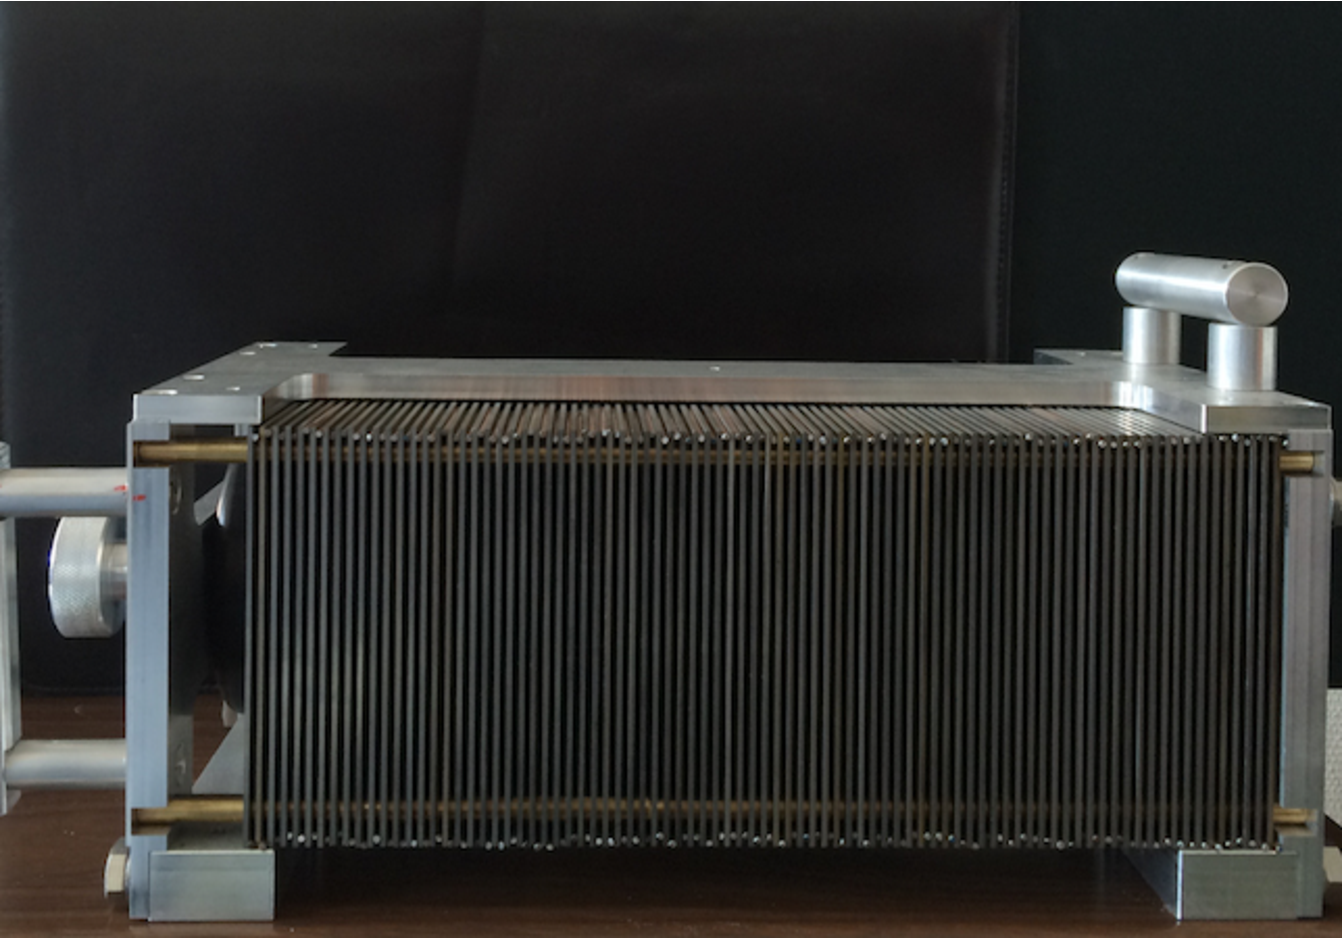
\includegraphics[width=1\textwidth, trim={0 0 0 0.5cm},clip = true]{03_GraphicFiles/chapter3_CLaRySproto/Collimator/Collimator.pdf}
\caption{Picture of the multi-slit tungsten collimator.}
\label{chap3::fig::collimatorPicture}
\end{subfigure}
\begin{subfigure}[t]{.5\textwidth}
\centering
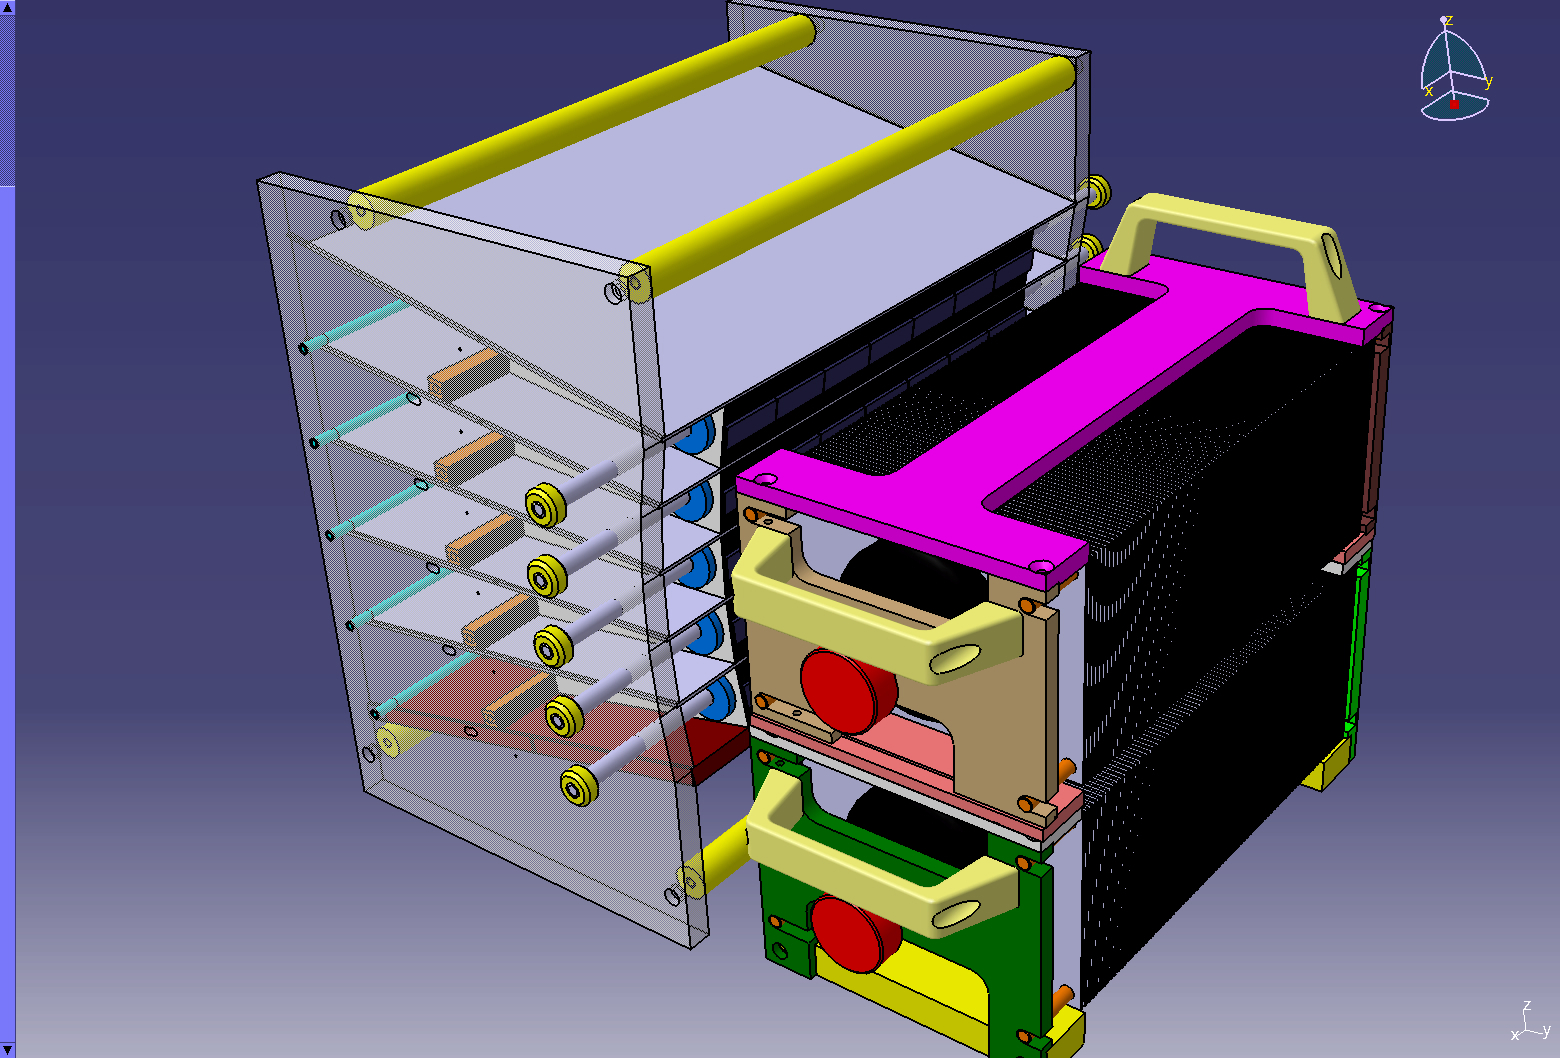
\includegraphics[width=1\textwidth]{03_GraphicFiles/chapter3_CLaRySproto/schemes/AbsoberCollimator.jpg}
\caption{Example of multi-collimated camera configuration: the two tungsten multi-slit collimators are placed in front of a 6$\times$5 \gls{bgo} block absorber setup in its mechanical support (see section~\ref{chap3::subsec::absorber})}
\label{chap3::fig::collimatorScheme}
\end{subfigure}
\caption{}
\label{chap3::fig::collimatorFig}
\end{figure} 


%%%%%%%%%%%%%%%%%%%%%%%%%%%%%%%%%%   ABSORBER  %%%%%%%%%%%%%%%%%%%%%%%%%%%%%%%%%%%%%%%%%%%%

\subsection{Absorber}\label{chap3::subsec::absorber}

The Compton and multi-collimated camera absorber was initially conceived as a very large surface plane composed of 96 \gls{bgo} blocks recovered from a dismantled \gls{pet} system HR+ by SIEMENS, documented in~\parencite{Adam1997, Brix1997}.\\ 
%%%From BGO paper %%%%%%%%
\gls{bgo} is one of the most used scintillators for gamma detection applications, thanks to a good energy resolution and a optimal gamma detection efficiency. Moreover, the absence of internal radioactivity which characterizes other scintillator materials employed in the same field (i.e.~\gls{lyso}, \gls{lso}), makes it suitable for low noise detectors, required by a Compton camera to reduce the amount of random coincidences, one of the main sources of background for the application in ion beam therapy monitoring~\parencite{Ortega2015}. As highlighted in~\parencite{HuesoGonzalez2015}, \gls{lyso} and \gls{lso} show overall better performances with respect to \gls{bgo} for what concerns energy, time and spatial resolution, due to an about 4 times higher light yield, but the gap is reduced for the detection of gamma rays in the prompt-gamma energy range (especially beyond 1~MeV). The limited cost of \gls{bgo} with respect to \gls{lso} and the comparable performances in the prompt-gamma energy range make it an optimal solution for prompt-gamma camera prototypes.\\
Each \gls{bgo} block has a surface of 3.5$\times$3.8~cm$^2$, with a thickness of 3.0~cm. The mono-block \gls{bgo} crystal is streaked in a 8$\times$8 pseudo-pixel matrix; a reflecting material is inserted between the pseudo-pixels to improve the light collection and optimize the spatial information accuracy via pixel separation. The read-out is achieved via four \gls{pm} tubes per block, composing a quartet, coupled to the block back surface. Thanks to the internal streaked structure of the block, the scintillation light is shared on the four \glspl{pm} depending on the pseudo-pixel where the interaction takes place (in case of multiple interactions more than 1 pseudo-pixel can be involved). The reconstruction of the position of interaction is done via Anger logic, i.e.~with a center of gravity calculation.\\
The whole set of recovered blocks was supposed to undergo a \enquote{reconditioning} process, including the \gls{pm} removal, the crystal back surface polishing with diamond-based abrasive tool, the single \glspl{pm} gain characterization and grouping in quartets with similar gains, the final re-coupling of the \glspl{pm} and block shielding.\\ A set of \enquote{reconditioned} blocks have been tested with the method described in section~\ref{chap3::sec::charMeasurements} and their performance have been compared to a set of original blocks. An overall degradation of the detection performance has been verified on all the tested \enquote{reconditioned} blocks, which showed lower amplitude output signals probably link to a reduction of the collected scintillation light. Various correction methods have been tested, with unsatisfactory results. According to the outcome of these tests, summarized in~\cite{Sandjong2017}, the collaboration finally opted to adapt the camera design for the use of original, \enquote{non-reconditioned} \gls{bgo} blocks.\\    
Thirty original blocks are now available to compose the absorber detector. In addition to the already presented features, it must be noticed that the lateral surfaces of the original blocks, as well as the half of the \gls{pm} length, are covered by a reflecting material which ensures the complete collection of the scintillation light. This is probably a component which was not well reproduced during the reconditioning process. The whole structure is then protected by a 1~mm thick aluminum foil, which also isolates from external light contamination.\\
Figure~\ref{chap3::fig::block_noPM} shows one \gls{bgo} block before the coupling to the \gls{pm} quartet: the streaked structure is clearly visible, as well as the white reflecting material separating the pseudo-pixels and the one surrounding the block lateral sides. As mentioned, the same material also covers part of the photo-multiplier tubes, as shown in picture~\ref{chap3::fig::originalBlock_noAl}, where the four \glspl{pm} are glued to the block back surface. The described aluminum cover is visible in figure~\ref{chap3::fig::originalBlock_withAl}, while in figure~\ref{chap3::fig::BGOblockScheme} a scheme of a block together with the related \gls{pm} quartet is given. The spatial reconstruction logic is also reported in the same figure. To be noticed that the streaked structure of the pseudo-pixels depends on their position in the block: the reflecting streak covers about three fourth of the block thickness for the for the lateral pseudo-pixels, while it is limited to half of the block thickness for the central ones.\\ 

\begin{figure}
\begin{subfigure}[b]{.5\textwidth}
\centering
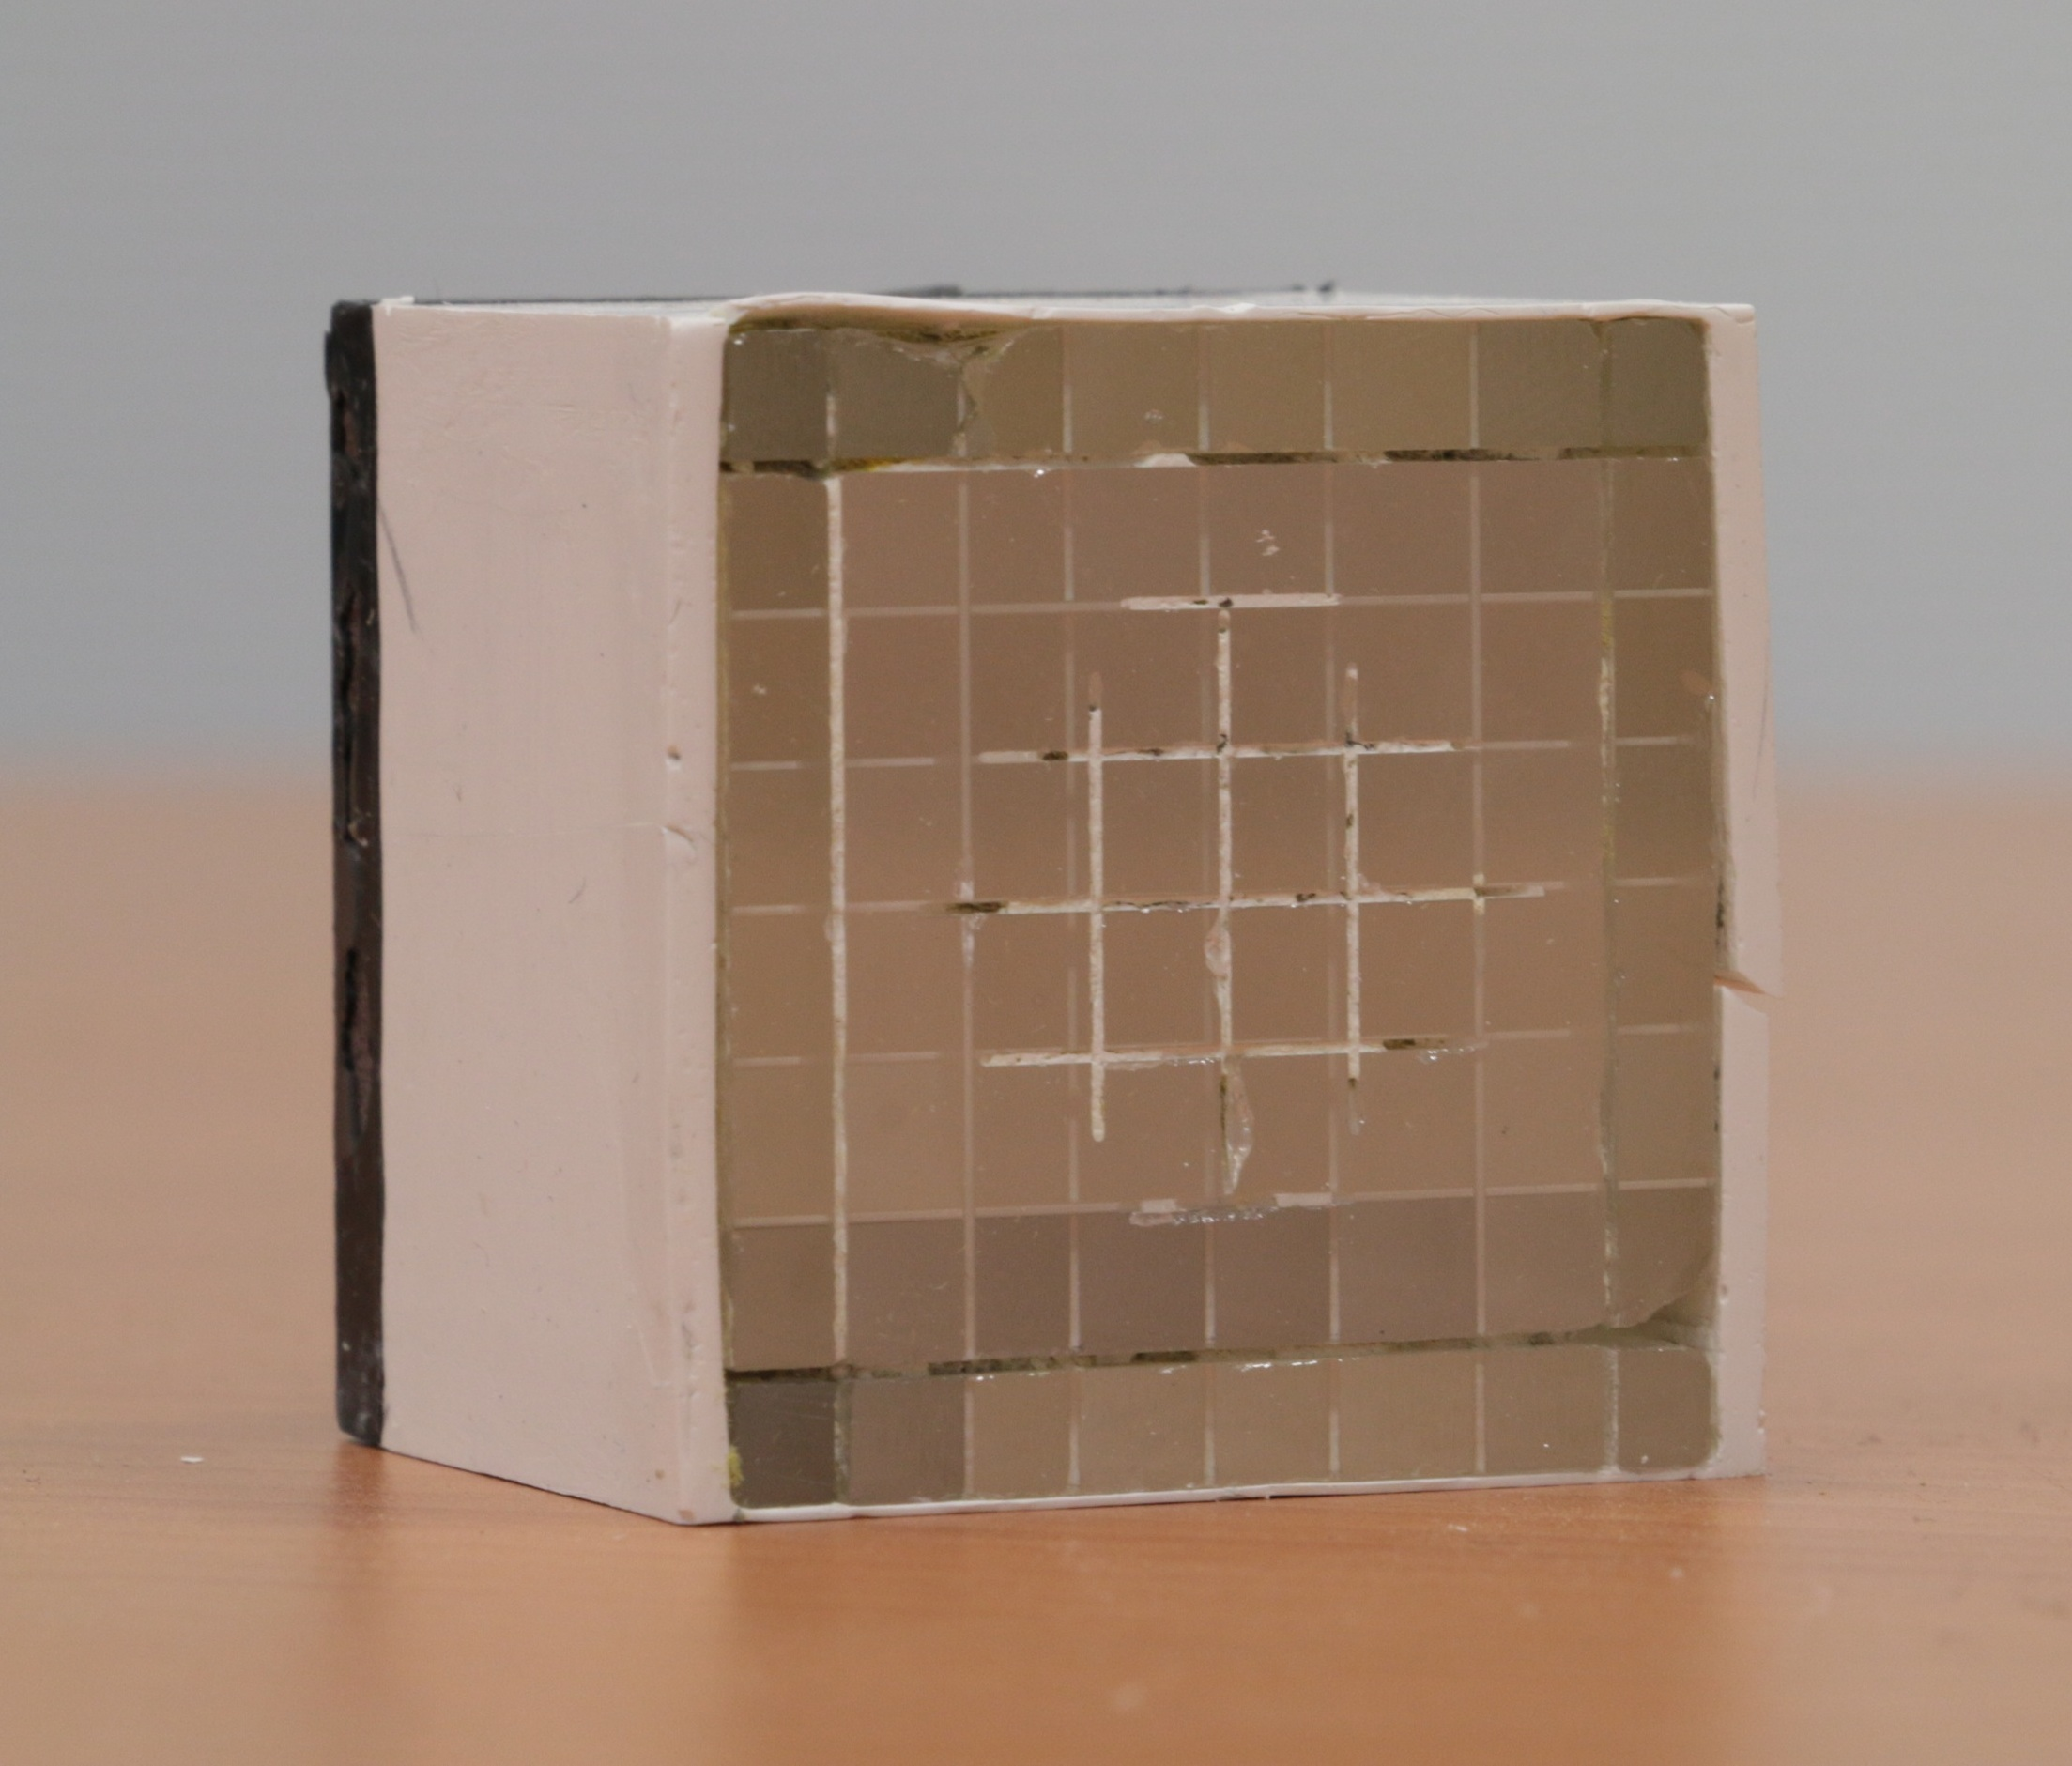
\includegraphics[width=1\textwidth, height=16em]{03_GraphicFiles/chapter3_CLaRySproto/Absorber/images/block_noPM}
\caption{\gls{bgo} raw block.}
\label{chap3::fig::block_noPM}
\end{subfigure}
\begin{subfigure}[b]{.5\textwidth}
\centering
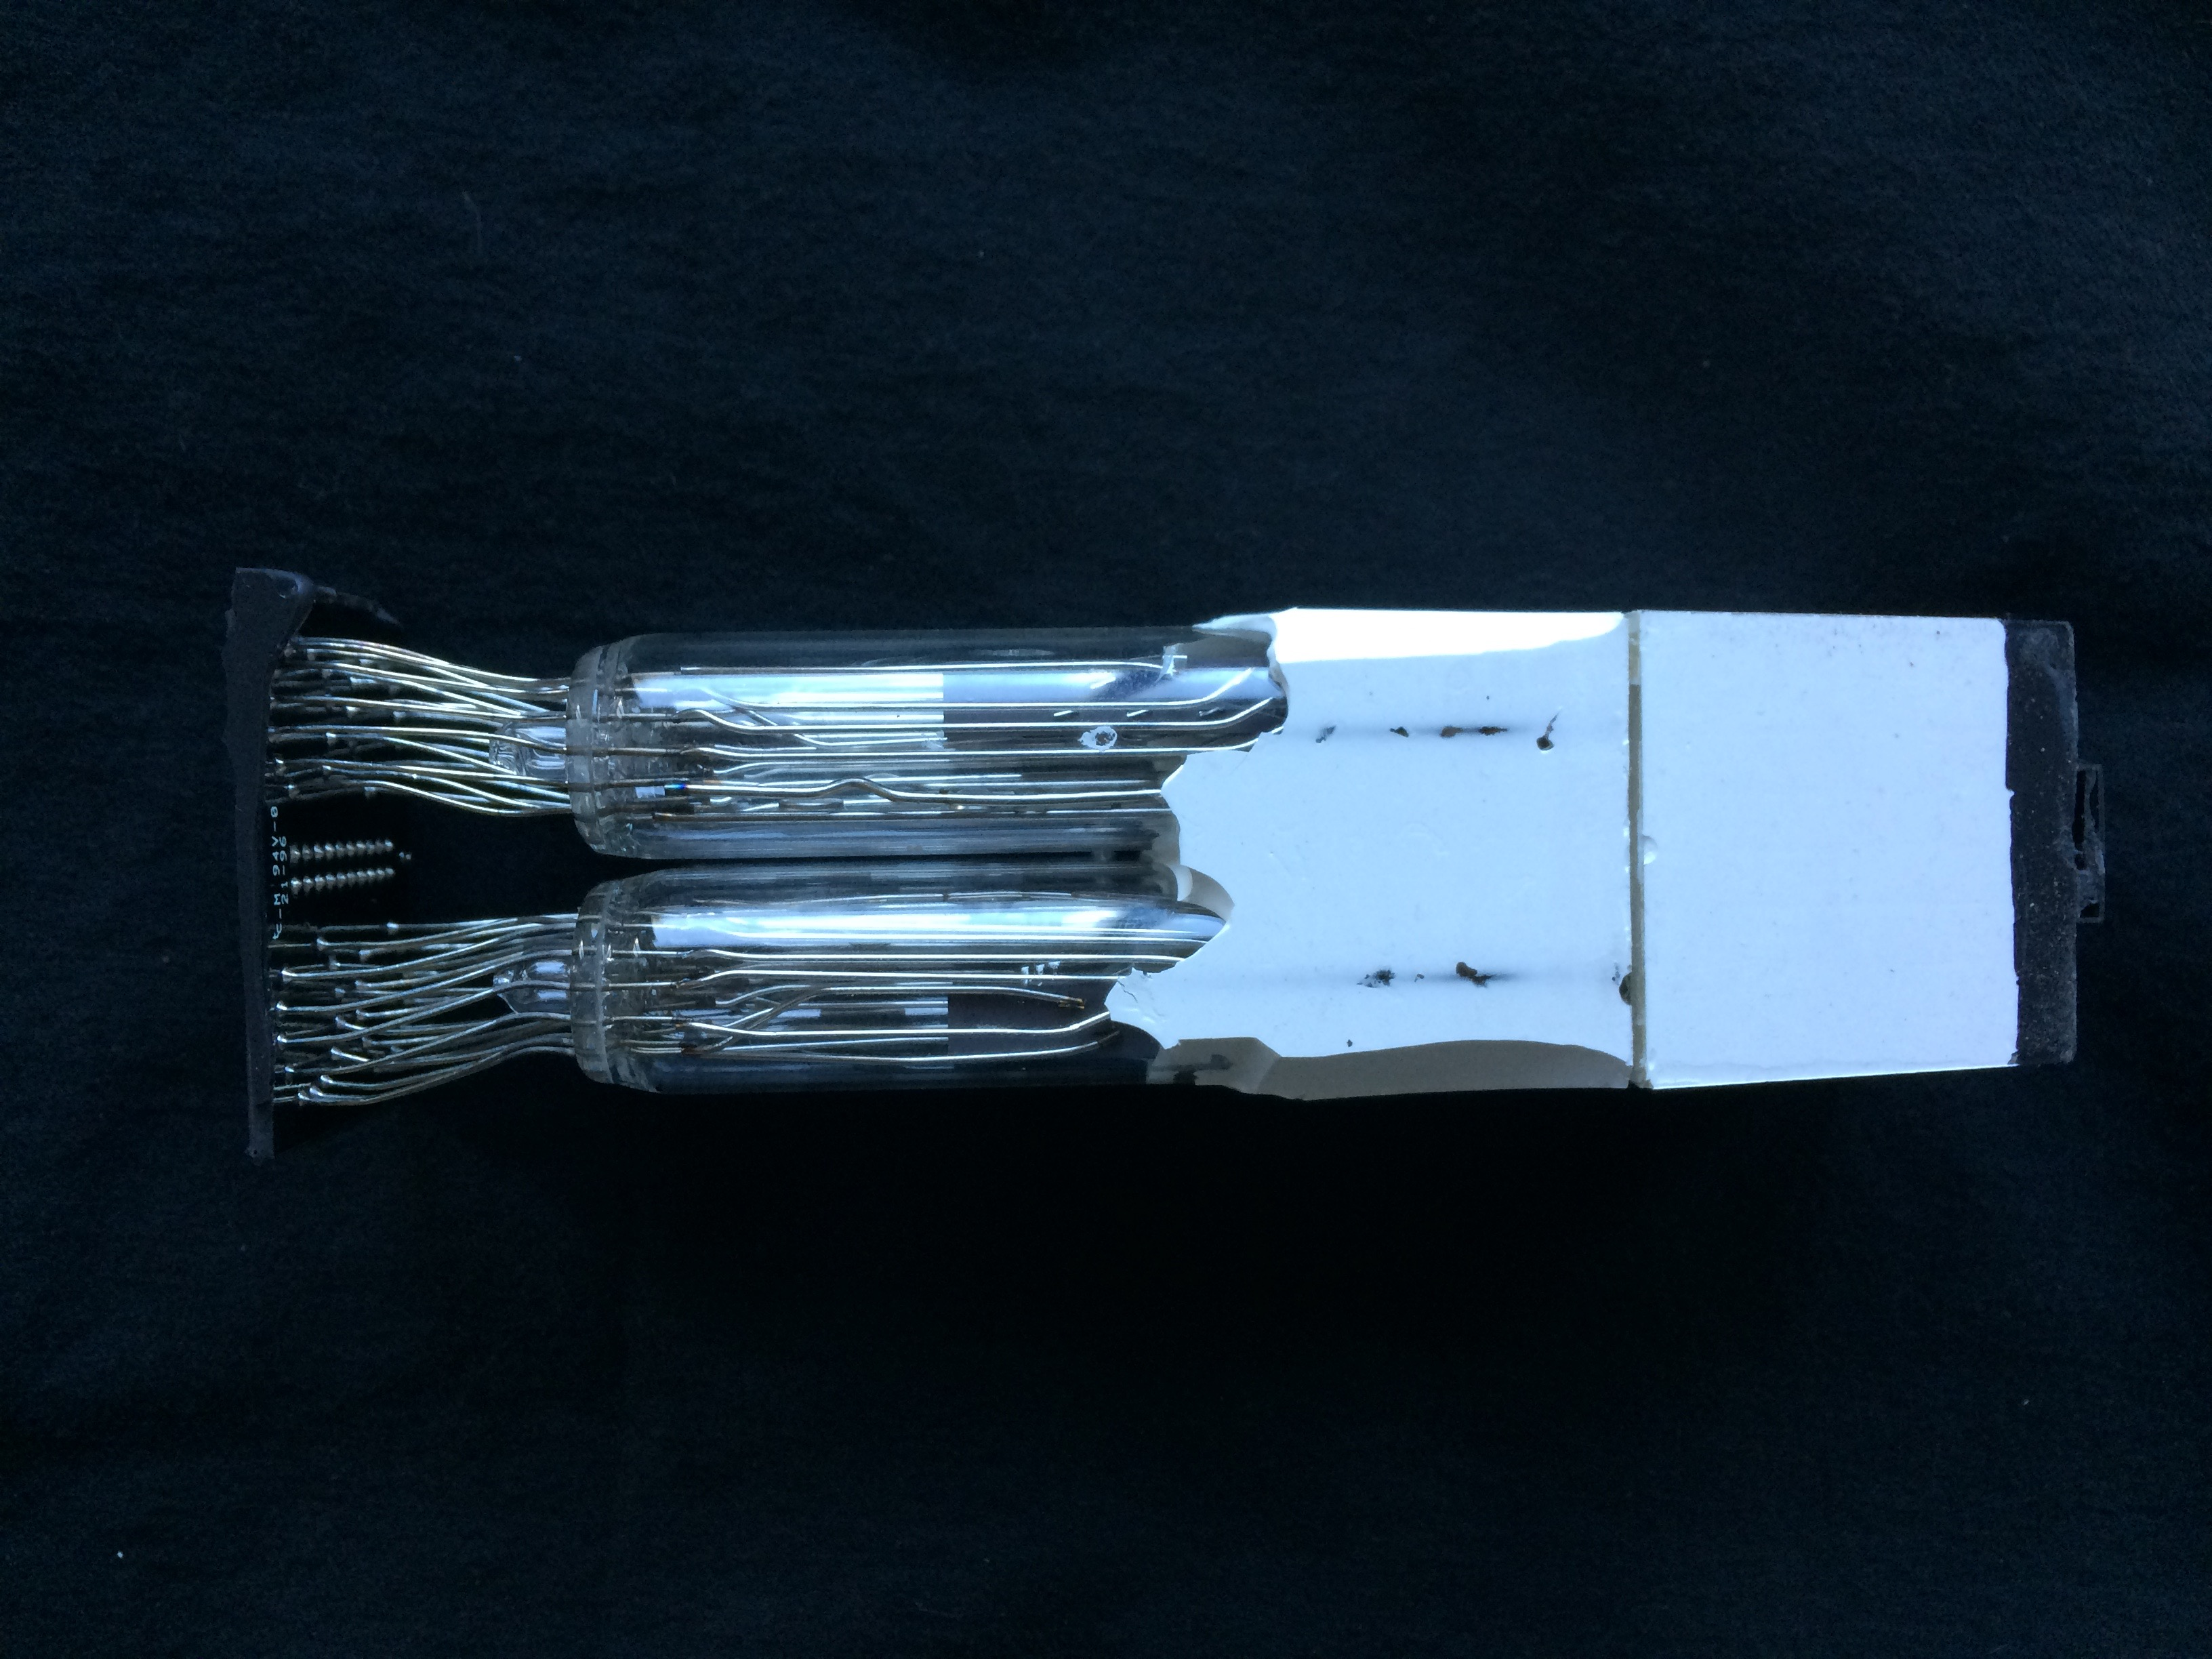
\includegraphics[width=1\textwidth, height=16em]{03_GraphicFiles/chapter3_CLaRySproto/Absorber/images/originalBlock_noAluminum}
\caption{\gls{bgo} crystal coupled to \gls{PM} quartet.}
\label{chap3::fig::originalBlock_noAl}
\end{subfigure}
\begin{subfigure}[b]{.5\textwidth}
\centering
\includegraphics[width=1\textwidth, height=16em]{03_GraphicFiles/chapter3_CLaRySproto/Absorber/images/originalBlock_withAluminum}
\caption{\gls{bgo} complete module with aluminum cover.}
\label{chap3::fig::originalBlock_withAl}
\end{subfigure}
\begin{subfigure}[b]{.5\textwidth}
\centering
\includegraphics[width=1\textwidth, height=16em]{03_GraphicFiles/chapter3_CLaRySproto/Absorber/block_scheme.pdf}
\caption{Scheme of a \gls{bgo} block and its spatial reconstruction logic.}
\label{chap3::fig::BGOblockScheme} 
\end{subfigure}
\caption{Absorber modules.}
\label{chap5::fig::BGO_block}
\end{figure}


\subsubsection{Absorber Front-End and read-out cards}\label{chap3::subsubsec::AbsorberFEcard}

A custom front-end card has been designed and produced by the \gls{lpc} research group and is used for the read-out of each \gls{bgo} block. The card is equipped with four voltage modulators which divide the provided high voltage on the 4 photo multiplier tubes. The voltage sent to each \gls{PM} can be mechanically tuned via screw-potentiometers on these modules. The card is equipped with differential output channels, through which the \gls{pm} signals are sent to the read-out card, called ASM card. A picture of the \gls{fe} card is given in figure~\ref{chap3::fig::FEcard}. To be noticed that 4 analog output channels has been added on some cards in order to allow laboratory tests with a signal treatment based on standard electronics modules, as described in section~\ref{chap3::sec::charMeasurements}. 

\begin{figure}
\begin{subfigure}[b]{.5\textwidth}
\centering
\includegraphics[width=1.1\textwidth, angle = -90]{03_GraphicFiles/chapter3_CLaRySproto/Absorber/images/FEcard}
\caption{Front-End card of the absorber \gls{bgo} detectors.}
\label{chap3::fig::FEcard_mod} 
\end{subfigure}
\begin{subfigure}[b]{.5\textwidth}
\centering
\includegraphics[width=1\textwidth]{03_GraphicFiles/chapter3_CLaRySproto/Absorber/ASMcard.jpg}
\caption{ASM card of the absorber \gls{bgo} detectors.}
\label{chap3::fig::ASMcard} 
\end{subfigure}
\caption{}
\label{chap5::fig::AbsorberCards}
\end{figure}

DESCRIPTION OF THE ASM CARD

\subsubsection{Absorber mechanical support}\label{chap3::subsubsec::AbsorberMechanics}

A first mechanical structure for the absorber detector was initially conceived by the \gls{lpc} group in order to hold up to 100 modules, foreseen by the original camera design. The reduction of the number of available blocks caused by the \enquote{reconditioning} process failure make necessary an adaptation of such a support. The new design has been carried out by the mechanics group of the \gls{ipnl} in order to be compact and flexible in terms of detection modules setup. Figure~\ref{chap3::fig::absorber_scheme} displays both a picture and a scheme of the absorber configuration with its mechanical support. The two lateral sides are built with \gls{pmma} boards connected by metal bars, and the \gls{bgo} blocks can be arranged in up to 5 rows of variable size, ranging from 3 to 7 blocks. Each block row is supported by a thin metal foil, designed to reduce at minimum the blocks separation and to respect the original ring geometry deriving from the SIEMENS \gls{pet} system. The blocks composing a row are then laterally pressed via two screws on the two sides of the structure, which can also be used to adapt the rows relative position horizontally. On the back side, a metal bar is added to avoid undesired movements, and the \gls{fe} cards are fixed with plastic pillars. The realized support results to be versatile, compact and adapted to the prototype tests for both the Compton camera (where a squared setup is preferred) and the multi-collimated one (where the collimator geometry must be fit by the absorber geometrical configuration).       

\begin{figure}
\begin{subfigure}[b]{.5\textwidth}
\centering
\includegraphics[width=1\textwidth, height=16em]{03_GraphicFiles/chapter3_CLaRySproto/Absorber/images/absorber_picture.JPG}
\caption{Picture of the absorber detector in its mechanical support.}
\label{chap3::fig::absorberPicture}
\end{subfigure}
\begin{subfigure}[b]{.5\textwidth}
\centering
\includegraphics[width=1\textwidth, height=16em]{03_GraphicFiles/chapter3_CLaRySproto/Absorber/images/Absorbeur.jpg}
\caption{Scheme of the absorber detector with its mechanical support.}
\label{chap3::fig::absorber30Scheme}
\end{subfigure}
\caption{Absorber front view with the \gls{bgo} block lines arranged in the mechanical support (left). Scheme of the \gls{bgo} absorber with its mechanical support (right).}
\label{chap3::fig::absorber_scheme}
\end{figure}

%%%%%%%%%%%%%%%%%%%%%%%%%%%%%%%%%%   HODOSCOPE  %%%%%%%%%%%%%%%%%%%%%%%%%%%%%%%%%%%%%%%%%%%%

\subsection{Beam tagging hodoscope}\label{chap3::subsec::hodoscope}

A beam tagging hodoscope is being developed in parallel to the two gamma cameras, mainly for background rejection and reconstruction optimization purposes [CIT]. As already mentioned, the detection of prompt-gammas (with mechanical or \enquote{electronical} collimation), is affected by the presence of other secondary particles produced during the ion beam irradiation, mainly neutrons. This background source can be efficiently identified and removed my applying \gls{tof} selection windows to the data acquisition. The \gls{tof} measurements can be performed using the accelerator radio-frequency signal as reference, but a direct beam detection results to be more accurate. An auxiliary detector is then needed before the beam interaction in the patient.\\ 
The \gls{clarys} hodoscope prototype is designed to provide space and time information about the incoming primary beam, particle by particle or bunch by bunch, depending on the beam intensity and detector efficiency and rate acceptance which must be characterized. In addition to the already explained use of the time information, a space primary particle tagging can be used to improve the reconstruction accuracy and constraint the possible reconstructed emission vertex in case of analytic reconstruction approach for both the multi-collimated and Compton cameras (see chapter~\ref{chap::2}).\\  
The detector under development is based on squared 1~mm$^{2}$ polystyrene scintillating fibers BCF-12, 140~mm in length, provided by Saint Gobain~\parencite{SaintGobain2017}. A picture of the hodoscope on its mechanical support (detailed in the following) is presented in figure~\ref{chap3::fig::HodoscopeMain}. The fibers are arranged into two perpendicular planes for a two-dimensional spatial information: each plane is composed of 128 fibers, for a total active area (for 2D measurements in coincidence) of 128$\times$128~mm$^{2}$. The active detector surface is completely covered with black reflective tape, which shields from external light. The scintillation light produced in the fibers by a ionizing particle deposing energy is transported to the read-out system via FORETEC optical fibers (1.55~cm diameter, 1~m length), which are connected to the scintillating fibers thanks to a custom mechanical support and to a proper gluing process (see figure~\ref{chap3::fig::HodoMounting}). Each scintillating fibers is read-out on both sides to optimize the detector efficiency and improve the time resolution which is not depending on the interaction position along the fiber with this configuration, so that the total number of read-out channels is 512. The signal read-out is ensured by 8 multi-anode \glspl{pm} Hamamatsu H8500~\parencite{Hamamatsu2006} shown in figure~\ref{chap3::fig::PMH8500}. The optical fibers are connected to the \gls{pm} anode surfaces through a plastic custom mask, shown in figure~\ref{chap3::fig::PMmask}. The \glspl{pm} are equipped with custom black boxes which operate as mechanical support and external light protection (see figure~\ref{chap3::fig::HodoMounting}). In order to provide further light isolation, the whole \gls{pm} boxes are covered with black tape.\\
The optical fibers are connected to the \glspl{pm} with the aim of increasing the maximum counting rate. 4 \glspl{pm} are dedicated to the read-out of the horizontal fibers, and 4 to the vertical ones, and the neighboring fibers are connected to different \glspl{pm}. An active area of 4$\times$4~mm$^{2}$ on the two planes is then read-out by all the 8 \glspl{pm}. Moreover, the two sides of the same scintillating fiber are connected on the same \gls{pm}. This fiber connection logic also improve the detector robustness; in case of problem on one \gls{pm}, only 1~mm each 4~mm is lost on a single plane, so that the detection of the beam is still possible on the whole active area.\\  
Each \gls{pm} is connected to a single custom \gls{fe} card. The hodoscope \gls{fe} cards have been developed by the \gls{ipnl} electronics group: their design is described in section~\ref{chap3::subsubsec::HodoFEcard}. 8 \gls{fe} cards are then used for the read-out, and the collected data are sent to the acquisition system described in section~\ref{chap3::subsec::cameraElectronicsDAQ}.

\begin{figure}[!htbp]
\centering
\includegraphics[width=0.6\textwidth]{03_GraphicFiles/chapter3_CLaRySproto/Hodoscope/Hodoscope_onTable.jpg}
\caption{\gls{clarys} scintillating fiber hodoscope on its 2-dimensional moving table.}
\label{chap3::fig::HodoscopeMain}
\end{figure}

\begin{figure}
\begin{subfigure}[t]{0.5\textwidth}
\centering
\includegraphics[width=1\textwidth]{03_GraphicFiles/chapter3_CLaRySproto/Hodoscope/Hodoscope_mounting.jpg}
\caption{Scintillating fiber hodoscope during mounting process.}
\label{chap3::fig::HodoMounting}
\end{subfigure}
\begin{subfigure}[t]{0.5\textwidth}
\centering
\includegraphics[width=1\textwidth]{03_GraphicFiles/chapter3_CLaRySproto/Hodoscope/hodoPMfiberConnection.pdf}
\caption{Scheme of the scintillating fiber connection to the \glspl{pm} (top) and of the double-sided fiber read-out (bottom).}
\label{chap3::fig::HodoPMfiberConn}
\end{subfigure}
\newline
\begin{subfigure}[t]{0.5\textwidth}
\centering
\includegraphics[width=1\textwidth]{03_GraphicFiles/chapter3_CLaRySproto/Hodoscope/H8500.png}
\caption{Hodoscope read-out \glspl{pm} Hamamatsu H8500.}
\label{chap3::fig::PMH8500}
\end{subfigure}
\begin{subfigure}[t]{.5\textwidth}
\centering
\includegraphics[width=1\textwidth]{03_GraphicFiles/chapter3_CLaRySproto/Hodoscope/Hodoscope_PMmask.JPG}
\caption{\gls{pm} plastic mask for optical fiber connection.}
\label{chap3::fig::PMmask}
\end{subfigure}
\caption{Details of the \gls{clarys} scintillating fiber hodoscope setup.}
\label{chap3::fig::HodoscopeParts}
\end{figure}


\subsubsection{Hodoscope Front-End card}\label{chap3::subsubsec::HodoFEcard}

The hodoscope is designed to tag in space and time the incoming beam ions, so that the signal read-out must be optimized to provide accurate time measurements and an high detection rate acceptance, with reduced dead time and detection efficiency close to 100\%. In particular, the design requirements include a maximum counting rate acceptance of 10$^{8}$~Hz per detection plane, with a time resolution of 1~ns~\parencite{Krimmer2014}.  The hodoscope \gls{fe} card shown in figure~\ref{chap3::fig::HodoscopeFEcard} has been developed by the \gls{ipnl} electronics group to fulfill the listed requirements. The Hamamatsu \gls{pm} is connected to the 64-channel connector (4 connectors of 16 channels each) and two custom \glspl{asic} are dedicated to the data first treatment (32 channels each).\\
  
\begin{figure}
\begin{subfigure}[t]{.3\textwidth}
\centering
\includegraphics[width=1\textwidth]{03_GraphicFiles/chapter3_CLaRySproto/Hodoscope/HodoCard1.jpg}
\caption{Hodoscope Front-End card.}
\label{chap3::fig::HodoscopeFEcard}
\end{subfigure}
\begin{subfigure}[t]{.7\textwidth}
\centering
\includegraphics[width=0.5\textwidth]{03_GraphicFiles/chapter3_CLaRySproto/Hodoscope/HodoScheme.png}
\caption{Hodoscope mechanical support scheme.}
\label{chap3::fig::HodoscopeSchemeMech}
\end{subfigure}
\caption{Hodoscope Front-End card developed at \gls{ipnl}.}
\label{chap3::fig::HodoPic}
\end{figure}

A first version of the \gls{fe} \gls{asic} has been developed in 2012 by the group \gls{micrhau} for the read-out of 8 channels (designed for the 32$\times$32 fiber hodoscope prototype described in section~\ref{chap3::subsubsec::SmallHodoProto}). The input part is composed of a current conveyor, and the output one has two sections: a current discriminator and a charge pre-amplifier for the charge measurements in test mode~\parencite{Deng2012, Deng2013}. In addition, the \gls{asic} gain can be tuned channel by channel, so that the response of each \gls{pm} output channel can be fine tuned with respect to the others.\\
The second version of the \gls{asic} includes all the features of the first version, with the addition of a \gls{tdc} based on a 160~MHz clock for a more accurate time tagging of the detected events. Moreover, a \gls{dll} is installed to divide the main clock in 32 intervals: for each event, the \gls{dll} state is stored in a 32 bit register and then encoded in a 5-bit Gray decoder. As a result, the \gls{tdc} has a 6.25~ns dynamics, with a sampling step of 195~ps and a time resolution of 58.8~ps \gls{rms}, for a maximum accepted rate of 10$^{8}$~Hz~\parencite{Deng2012b}.\\
The third and final \gls{asic} version, called HODOPIC, is adapted to the big size hodoscope (512 read-out channels), with the extension to 32 channels and with the \gls{tdc} implemented on the second version. An external \gls{adc} is used for the charge measurement in test mode for a single channel, selected via slow control. All the \gls{asic} outputs are sent to a \gls{fpga} installed on the card for the actual time measurement and data decoding. The \gls{fpga} finally handles the data transmission to the acquisition system, depending on the card version.\\
A first card has been developed to test the first \gls{asic} version with the 32$\times$32 fiber hodoscope. It is based on a \gls{fpga} Altera Cyclone III~\parencite{Altera2012} and on 9 \glspl{asic}, with a LabVIEW acquisition. A single card is enough for the read-out of the complete small hodoscope prototype. This first setup has been tested on beam at the \gls{ganil} and the \gls{hit}, and a sub-ns time resolution has been verified, together with the expected 1~mm spatial resolution on the two fiber planes and an efficiency of more then 90\% at a 10$^{6}$ acquisition rate.\\
The second prototype of the card, shown in figure~\ref{chap3::fig::HodoscopeFEcard}, has been adapted to the 512-channel hodoscope described in the previous section and to the gamma camera acquisition system described in~\ref{chap3::subsec::cameraElectronicsDAQ}: each card has two HODOPIC \glspl{asic}, 32 channels each, so that it is designed for the read-out of a single 64-anode \gls{pm}. 8 cards are then needed for the read-out of the whole hodoscope. This version is based on a \gls{fpga} Altera StratixII GX~\parencite{Altera2009}, and the connection to the acquisition is ensured by a 3~Gbit/s optical link. 4 digital input-output channels are installed for test and validation purpose, together with an Ethernet port.\\
Further details about the different card versions and the applied validation tests can be found in~\cite{Chen2017}.\\
The hodoscope card firmware has been developed in 2017 and tested in simplified versions on beam, as detailed in chapter~\ref{chap::6}.
           

\subsubsection{Hodoscope mechanical support}\label{chap3::subsubsec::HodoMechanics}

The beam tagging hodoscope is set between the beam nozzle and the patient and requires a dedicated mechanical support. In order to profit of the large active area and to be able to remotely control the hodoscope position in the beam transverse plane, the detector is mounted on a 2-dimensional moving table (see the picture in figure~\ref{chap3::fig::HodoscopeMain}), which also supports the \gls{fe} cards. Detector and \gls{fe} cards are then integral and translate together. A scheme of the moving table is given in figure~\ref{chap3::fig::HodoscopeSchemeMech}.\\
The 2-axis table is provided by Beijing Winner Optical Instruments; it is composed of two motorized linear stages, connected via a right angle bracket. The two stages have a moving range of 30~cm each and the stepper motors have a step resolution of 20~\charmum. The employed motor controller is a Newport XPS-Q8~\parencite{Newport2017}, equipped with 8 channels for the simultaneous control of a maximum of 8 motors. The movements are steered with an online interface or with a LabVIEW based program, which will be integrated in the final setup of the slow control software under development with the cameras.

\subsubsection{Small hodoscope prototypes}\label{chap3::subsubsec::SmallHodoProto}
Before the production of the large active surface hodoscope prototype described in section~\ref{chap3::subsec::hodoscope}, two smaller prototypes have been produced and tested in order to assess the potential of such a kind of detector for the required application. The first and simplest version consisted of one single scintillating fiber per plane, and the readout was performed with two \gls{pm} tubes directly coupled to the scintillating fibers, without optical fibers. A picture of this prototype is given in figure~\ref{chap3::fig::singleFibHodo}. This simple version of the detector has been used as a demonstrator of the basic detection principle.\\ 

\begin{figure}
\begin{subfigure}[t]{.5\textwidth}
\centering
\includegraphics[width=0.8\textwidth]{03_GraphicFiles/chapter3_CLaRySproto/Hodoscope/hodo2.jpg}
\caption{Hodoscope small prototype, 1$\times$1 scintillating fibers.}
\label{chap3::fig::singleFibHodo}
\end{subfigure}
\begin{subfigure}[t]{.5\textwidth}
\centering
\includegraphics[width=0.8\textwidth]{03_GraphicFiles/chapter3_CLaRySproto/Hodoscope/hodo32_withCard.jpg}
\caption{Hodoscope small prototype, 32$\times$32 scintillating fibers.}
\label{chap3::fig::Hodoscope32}
\end{subfigure}
\caption{Hodoscope small prototypes.}
\label{chap3::fig::HodoSmall}
\end{figure}

A second small size version of the final detector has been produced with almost the same features as the large area prototype but with simplified read-out logic. It is equipped with two perpendicular planes of 32 1~mm$^{2}$ scintillating fibers each (Saint Gobain BCF-10~\parencite{SaintGobain2017}), with a length of 4~cm and a total active area for a 2D read-out of 32$\times$32~mm$^{2}$. As in the big hodoscope, the scintillating fibers are coupled to FORETEC optical fibers which transfer the scintillation light to 4 Hamamatsu H8500 \glspl{pm}. 16 channels per \gls{pm} are used, so that 2 \glspl{pm} are dedicated to the horizontal fibers and 2 to the vertical ones, and the signal read-out is performed on a single side of the scintillating fibers. As the total number of read-out channels is 64, a single \gls{fe} card is enough for the whole detector. In figure~\ref{chap3::fig::Hodoscope32} the 32$\times$32-fiber hodoscope prototype is shown together with its \gls{fe} card; 4 connections cables (16 channels each) are used to couple the \glspl{pm} to the \gls{fe} card.\\
The 32$\times$32-fiber hodoscope prototype has been tested in 2014 on proton and carbon ion beams (at the \gls{ganil} - 75~MeV/u $^{13}$C, \gls{hit} - protons and carbon ions at various energy, \gls{ipno} - 25~MeV protons) with the first version of the \gls{fe} card (see section~\ref{chap3::subsubsec::HodoFEcard}): an efficiency of more than 90\% has been retrieved, with a time resolution of 1~ns \gls{fwhm} (timing measurements performed with respect to the accelerator high frequency signal). Some more details about this beam tests results are given in chapter~\ref{chap::6}. The final version of the \gls{fe} card has been also tested with this detector, and the test description and results are presented in chapter~\ref{chap::6}.  
   

%%%%%%%%%%%%%%%%%%%%%%%%%%%%%%%%%%   ELECTRONICS/DAQ  %%%%%%%%%%%%%%%%%%%%%%%%%%%%%%%%%%%%%%%%%%%%

\subsection{Camera electronics and acquisition system}\label{chap3::subsec::cameraElectronicsDAQ}

\begin{figure}
\begin{subfigure}[t]{.35\textwidth}
\centering
\includegraphics[width=1\textwidth]{03_GraphicFiles/chapter3_CLaRySproto/Electronics_Acquisition/uTCAcrate_1.jpg}
\caption{}
\label{chap3::fig::uTCAcrate}
\end{subfigure}
\begin{subfigure}[t]{.28\textwidth}
\centering
\includegraphics[width=1\textwidth, angle = -90, trim={0 0.2cm 0 0.2cm}, clip = true]{03_GraphicFiles/chapter3_CLaRySproto/Electronics_Acquisition/AMC40_ipnl_top.jpg}
\caption{}
\label{chap3::fig::AMC40}
\end{subfigure}
\begin{subfigure}[t]{.36\textwidth}
\centering
\includegraphics[width=1\textwidth]{03_GraphicFiles/chapter3_CLaRySproto/Electronics_Acquisition/THOR.pdf}
\caption{}
\label{chap3::fig::THOR}
\end{subfigure}
\caption{}
\label{chap3::fig::AcquisitionSystem}
\end{figure}


\begin{figure}[!htbp]
\centering
\includegraphics[width=0.9\textwidth]{03_GraphicFiles/chapter3_CLaRySproto/Electronics_Acquisition/acqLogic_complete.pdf}
\caption{Schematic view of the Compton camera acquisition system. For the multi-collimated camera, the trigger and pre-trigger signals are the same.}
\label{chap3::fig::DAQscheme}
\end{figure}


%%%%%%%%%%%%%%%%%%%%%%%%%%%%%%%%%%   SOFTWARE  %%%%%%%%%%%%%%%%%%%%%%%%%%%%%%%%%%%%%%%%%%%%

\subsection{Camera slow control, acquisition and monitoring software}\label{chap3::subsec::cameraSoftware}

%%%%%%%%%%%%%%%%%%%%%%%%%%%%%%%%%%   MECHANICAL SUPPORT  %%%%%%%%%%%%%%%%%%%%%%%%%%%%%%%%%%%%%%%%%%%%

\subsection{Camera integration and mechanical support}\label{chap3::subsec::CameraMechanics}

\begin{figure}
\begin{subfigure}[t]{.5\textwidth}
\centering
\includegraphics[width=1\textwidth, trim= {1cm 0 1cm 0}, clip = true, height=5cm]{03_GraphicFiles/chapter3_CLaRySproto/Mechanics/TableCameraSchemeBlue.jpg}
\caption{}
\label{chap3::fig::schemeTable}
\end{subfigure}
\begin{subfigure}[t]{.5\textwidth}
\centering
\includegraphics[width=1\textwidth]{03_GraphicFiles/chapter3_CLaRySproto/Mechanics/Table.JPG}
\caption{}
\label{chap3::fig::pictureTable}
\end{subfigure}
\caption{}
\label{chap3::fig::CameraIntegration}
\end{figure}

%%%%%%%%%%%%%%%%%%%%%%%%%%%%%%%%%%   CHARACTERIZATION MEASUREMENTS  %%%%%%%%%%%%%%%%%%%%%%%%%%%%%%%%%%%%%%%%%%%%

\section{Camera component characterization and development status}\label{chap3::sec::charMeasurements}

As detailed in the previous sections, the \gls{clarys} \gls{tof} gamma cameras are equipped with various detector components with very different features. Each part must be separately studied in order to characterize its behavior and allow the final camera integration and operation.\\
I mostly worked on the beam tagging hodoscope and on the \gls{bgo} absorber, and in the next paragraphs the performed measurements are described in details. Concerning the scatterer stack, the results achieved before the beginning of my PhD thesis are briefly described for the sake of completeness.\\
The results presented in this section also introduce the following one (~\ref{chap3::sec::Next}), where all the development steps still needed for a clinical implementation of the cameras are explained.\\

\subsection{Hodoscope \glspl{pm} characterization}\label{chap3::subsec::hodoPMchar}         

The beam tagging hodoscope read-out is performed via 8 multi-anode \glspl{pm}, Hamamatsu H8500~\parencite{Hamamatsu2006}, shown in figure~\ref{chap3::fig::PMH8500}. In order to guarantee a uniform response of the whole detector active area, composed of 256 scintillating fibers, the \glspl{pm} must be previously characterized in terms of gain with a light source of fixed and known wave-length and intensity. The source selected for the measurements is a blue \gls{led} (Hewlett-Packard HLMP-CB), installed on the test-bench shown in figure~\ref{chap3::fig::hodo_testBenchPM} and described in the following. The test-bench has been developed by the \gls{lpc} group (see~\cite{Gaglione2013}) and adapted at the \gls{ipnl} to a different acquisition system.\\
The goal of the characterization measurements is to trace a gain map of the whole \gls{pm} surface, with the aim of storing calibration data to be used to both tune the \gls{pm} working parameters (supply voltage and threshold) and correct the collected data. This is achieved by scanning the \gls{pm} photo-cathode surface with the \gls{led}. The \gls{led} is so mounted on a motorized double-axis table, controlled by two G203V stepper modules provided by GeckoDrive Motor Controls~\parencite{GeckoDrive2010}. The two axes have a total range of 20~cm each, and the step resolution achieved by the controllers is 20~\charmum. A metal support is set on the table in order to fix the \gls{led}. It produces light pulses synchronized with a pulse generator, which is also used as trigger signal for the acquisition system, as detailed later. The light pulse produced by the \gls{led} is split into two pulses with a 45\textdegree{} mirror: one pulse is sent to the H8500 \gls{pm} to be tested via optical fiber, in order to obtain a light beam perpendicular to the cathode surface (\gls{fwhm} beam width estimated in 0.5~mm), the second one is detected by an Hamamatsu R5600 \gls{pm}~\parencite{Hamamatsu1995}, used as reference for the correction of \gls{led} temperature fluctuations. The \gls{pm} under tests if fixed below the optical fiber output with a plastic support, not connected to the moving table. The whole described system is contained in a black box for external light shielding.\\
The output signals from the H8500 \gls{pm} are initially amplified by custom pre-amplification cards: 8 cards are available and have been characterized in terms of amplification gain. Once amplified, the signals H8500 \gls{pm}, together with the output of the reference \gls{pm}, are sent to the acquisition system composed of a National Instrument PXI Express 1082~\parencite{NationalInstruments2010} equipped with two 8-channel flash \gls{adc} modules (NI PXI-5105) and a two-channel ultra-fast digitizer (NI PXI-5154). The flash \gls{adc} modules have a maximum sampling rate of 60~MHz and are used for the read-out of the H8500 \gls{pm} signals, while the ultra-fast digitizer, able to sample at a frequency up to 1~GHz, is used for the reference \gls{pm}.\\
The acquisition and control software is developed with LabVIEW (2009) installed on the PXI; a picture of the software user interface is shown in figure~\ref{chap3::fig::hodo_LabView}. The PXI receives the signals form the two \glspl{pm} and is also connected to the table stepper modules, so that the LabVIEW software can handle and synchronized data acquisition and table movements. The table movements can be automatized via LabVIEW macros, where step size, number and direction are stored and then used for the acquisition. The acquisition trigger, as mentioned, is given by the pulse generator which also control the light pulses of the \gls{led}; in this way, a fixed number of pulses per table position can be recorded, and the measurement process is completely automatic. During the acquisition, the LabVIEW software automatically correct the collected data according to the reference \gls{pm} signal amplitude and to the pre-amplification card gain.\\
Given the limited number of flash \gls{adc} channels, only 16 \gls{pm} pixels can be characterized per acquisition; four acquisitions are needed to scan the complete \gls{pm} surface.\\
 
\begin{figure}
\begin{subfigure}[t]{1\textwidth}
\centering
\includegraphics[width=0.7\textwidth]{03_GraphicFiles/chapter3_CLaRySproto/Hodoscope/testBenchPM.jpg}
\caption{}
\label{chap3::fig::hodo_testBenchPM}
\end{subfigure}
\newline
\begin{subfigure}[t]{.5\textwidth}
\centering
\includegraphics[width=1\textwidth, height = 5.cm]{03_GraphicFiles/chapter3_CLaRySproto/Electronics_Acquisition/PXI_ipnl.jpg}
\caption{}
\label{chap3::fig::PXI_NI}
\end{subfigure}
\begin{subfigure}[t]{.5\textwidth}
\centering
\includegraphics[width=1\textwidth]{03_GraphicFiles/chapter3_CLaRySproto/Hodoscope/hodoTests.jpg}
\caption{}
\label{chap3::fig::hodo_LabView}
\end{subfigure}
\caption{}
\label{chap3::fig::hodoPMtest}
\end{figure}

Each performed acquisition is set to scan a matrix of 4$\times$4 \gls{pm} pixels, and safety margins are arranged on the \gls{pm} sides in order to ensure a complete surface irradiation. As shown in the schematic view of the \gls{pm} in figure~\ref{chap3::fig::hodoPMscheme}, the total \gls{pm} size is 52$\times$52~mm$^{2}$, for an active area of about 49$\times$49~mm$^{2}$. The active area of the pixels on the borders is slightly wider than the central ones. In order to optimize the measurement process, a preliminary analysis has been done for the definition of the needed step length, and the details are reported in~\cite{Coudurier2015}. A trade-off between measurement accuracy, required time and collected data size has been found with a step of 800~\charmum, so that each pixel is scanned with approximately 64 measurement points and the transition between neighboring pixels can be appreciated. To be noticed that for each irradiated point, 100 \gls{led} pulses are sent to the detector and the average amplitude value is  calculated and collected.\\  
The 8 Hamamatsu \glspl{pm} have been completely scanned with and without the optical fiber mask used in the hodoscope and shown in figure~\ref{chap3::fig::PMmask}, and the results are shown here for one reference \gls{pm}. A complete result database has been created for calibration purpose.\\

\begin{figure}
\begin{subfigure}[t]{.5\textwidth}
\centering
\includegraphics[width=1\textwidth]{03_GraphicFiles/chapter3_CLaRySproto/Hodoscope/PM_specs_mod.pdf}
\caption{}
\label{chap3::fig::hodoPMscheme}
\end{subfigure}
\begin{subfigure}[t]{.5\textwidth}
\centering
\includegraphics[width=1\textwidth]{03_GraphicFiles/chapter3_CLaRySproto/Hodoscope/scan_logic.pdf}
\caption{}
\label{chap3::fig::hodoPMscanScheme}
\end{subfigure}
\caption{}
\label{chap3::fig::hodoScanDetails}
\end{figure}


\begin{figure}
\begin{subfigure}[t]{.5\textwidth}
\centering
\includegraphics[width=1\textwidth, height = 5.8cm ]{03_GraphicFiles/chapter3_CLaRySproto/Hodoscope/PMchar/2Dmap_noMask.pdf}
\caption{}
\label{chap3::fig::hodoPMchar2DnoMask}
\end{subfigure}
\begin{subfigure}[t]{.5\textwidth}
\centering
\includegraphics[width=1\textwidth, height = 5.8cm ]{03_GraphicFiles/chapter3_CLaRySproto/Hodoscope/PMchar/2Dmap_withMask.pdf}
\caption{}
\label{chap3::fig::hodoPMchar2DnoMask}
\end{subfigure}
\caption{}
\label{chap3::fig::hodoPMchar2Dmaps}
\end{figure}





\subsection{Hodoscope fiber test with electron source}\label{chap3::subsec::hodoBetatest}


\subsection{Absorber \gls{bgo} blocks characterization}\label{chap3::subsec::absBGOchar}

The \gls{bgo} modules composing the Compton and multi-collimated camera absorber have been recovered form a SIEMENS \gls{pet} system: they have been originally optimized for the detection of 511~keV photons from positron annihilation, and they have to be tested for the new gamma detection system, which must be able to deal with photons in the prompt-gamma energy range, i.e.~from some hundreds of keV to a few MeV.\\ 
Each block must be characterized in terms of spatial and energy response, and the read-out \glspl{pm} have to be calibrated to obtain a uniform response on the whole block surface (see section~\ref{chap3::subsec::absorber} for the detector description). The employed method relies on the work presented in~\cite{Rogers1994} and~\cite{Tornai1994} and on the calibration process described in~\cite{Golnik2015} and~\cite{HuesoGonzalez2015}, and has been extended with more refined features.\\
The measurements are performed with the irradiation with gamma sources, emitting photons at defined energies: in particular, we used 511~keV and 1275~keV photons from a $^{22}$Na source, and the two photons emitted by a $^{60}$Co source, at energies of 1173~keV and 1332~keV.\\
The employed $^{22}$Na source is a cylindrical source with a diameter of 1~cm, and an activity of about 400~kBq: it has been placed at a distance of about 5~cm from the block entrance surface, with the center of the source facing the center of the block transverse surface. The $^{60}$Co source has been installed in a lead cylindrical container (12~cm radius and 35~cm height), equipped with three different apertures: point-like (2$\times$2~mm$^2$), linear (2$\times$50~mm$^2$) and squared (50$\times$50~mm$^2$). The design of the lead container has been studied in simulation to ensure the proper radiation protection, and produced according to the specifications defined by the \gls{ipnl} mechanics group. The activity of the $^{60}$Co source is about 1.7~MBq, and the square shape has been used to obtain an homogeneous irradiation of the \gls{bgo} block, with the block set with the center of the entrance surface corresponding to the source position, at a distance of 12~cm.\\
The signals produced by the four \glspl{pm} of each block are collected via four analog outputs on the front-end card (see picture~\ref{chap3::fig::FEcard_mod}). The four retrieved signals per event are treated via standard \gls{nim} modules in order to be adapted to the acquisition systems and measurement purposes.\\
Two different acquisition systems have been used for this characterization work. First, the PXIe described in section~\ref{chap3::subsec::hodoPMchar} with its two flash \gls{adc} read-out modules, 8 channels each, is used for the spatial and energy characterization and calibration of the tested blocks. The raw signals coming from the four \glspl{pm} are amplified and shaped via \gls{nim} modules, which were fine tuned via a pulse generator in order to adapt the amplification factor of each channel (an amplification factor of about 50 has been applied to the raw signals). The amplified signals are then split in order to be treated for trigger purpose. The trigger for the acquisition is based on the sum of the four signals, and a fixed threshold is applied for background rejection. The employed discriminator provides the logical trigger signal, which is sent to the trigger input of the \gls{adc} modules on the PXI. The four amplified signals, conveniently delayed, are sent as inputs to the \gls{adc} modules on the PXI, together with the sum signal which is used for experimental verification of the acquisition setup. A LabVIEW based acquisition software, developed for this particular application by the \gls{ipnl} group, provides real time event visualization together with a partial, on-line spatial reconstruction of the events, and stores them in text files for further analysis. A second threshold can be set at the software level in case particular selections are needed during the acquisition, otherwise the event selection is performed at the analysis stage.\\
Concerning the timing characterization measurements, an eight-channel signal digitizer at 3.2~GS/s has been employed for high time resolution acquisitions. The so called WaveCatcher, shown in figure~\ref{chap3::fig::WaveCatcher}, has been developed by the \gls{lal} in Orsay and the \gls{irfu} in CEA-Saclay, and its features are detailed in~\cite{Breton2014}. The digitizer is connected to the acquisition PC via USB cable, and the data read-out and storage is performed thanks to a custom acquisition software.  The measurements are based on the coincidence detection of back-to-back 511~keV photons emitted by a $^{22}$Na radioactive source, in order to be able to compare the time response of the tested \gls{bgo} block to a reference fast timing scintillator. An external trigger is then provided to the WaveCatcher by treating the \gls{bgo} block and reference scintillator signals with logic coincidence \gls{nim} modules, after proper discrimination. Further details are given in section~\ref{chap3::subsubsec::absTimeMethod}.

\begin{figure}
\begin{subfigure}[t]{.45\textwidth}
\centering
\includegraphics[width=1\textwidth]{03_GraphicFiles/chapter3_CLaRySproto/Electronics_Acquisition/WaveCatcher.jpg}
\caption{}
\label{chap3::fig::WaveCatcher}
\end{subfigure}
\begin{subfigure}[t]{.55\textwidth}
\centering
\includegraphics[width=1\textwidth]{03_GraphicFiles/chapter3_CLaRySproto/Absorber/images/coincidence_timing_scheme_complete.pdf}
\caption{Scheme of the time response characterization test-bench.}
\label{chap3::fig::BGOtime_meas_scheme}
\end{subfigure}
\caption{}
\label{chap3::fig::BGO_timingDaq}
\end{figure}

\subsubsection{Space and energy calibration and characterization}\label{chap3::subsubsec::absSpaceEnMethod}

The space and energy calibration process is mainly divided into four parts:
\begin{itemize}
\item \underline{$^{22}$Na irradiation}: the block is irradiated with the sodium source and the raw \gls{adc} distributions for the four \glspl{pm} are retrieved. The highest \gls{adc} values are taken as reference to equalize the distributions. Four energy calibration factors are extracted and used to the data correction; this correction corresponds to a \gls{pm} gain equalization.

\item \underline{$^{60}$Co irradiation}: once the calibration factor are extracted thanks to the $^{22}$Na irradiation data, the block is exposed to the $^{60}$Co source. The collected data are analyzed as in the previous step and calibrated according to the already calculated correction factors. The energy spectrum, the mono-dimensional spatial projections and the flood map (two-dimension position map) are produced.

\item \underline{Pixel identification}: the custom algorithm briefly described in paragraph~\ref{chap3::subsubsec::absPixel_ID_algo} has been developed to identify the pseudo-pixel positions on the flood map. It is applied to the $^{60}$Co irradiation data and the pseudo-pixel position map is stored. 

\item \underline{Pixel energy calibration}: the $^{22}$Na irradiation data are re-analyzed in this last calibration step in order to assign each interaction to a single pseudo-pixel according to the pixel position map obtained with the $^{60}$Co data. The energy spectrum of each pixel can be then produced and the two identified peaks (corresponding to the two photon energies emitted by the sodium source - 511~keV and 1275~keV) can be used to equalize the pseudo-pixel response. The sum of all the pixels spectra produces the block energy spectrum. At this stage, the \gls{adc} channel values are calibrated to obtain the absorbed energy values in keV.     
\end{itemize}

It is worth to notice that the $^{60}$Co irradiation is useful for the pixel identification given the high energy and narrow energy range of the emitted photons. The equalization factors obtained with the sodium source irradiation have been verified to be consistent with the $^{60}$Co irradiation data, as expected. In addition to this, the pixel position map obtained with the $^{60}$Co irradiation data has been verified to fit with the $^{22}$Na data, which presents larger distributions around the pseudo-pixel center. The whole method results to be robust.  

\subsubsection{Pixel identification and energy calibration algorithm}\label{chap3::subsubsec::absPixel_ID_algo}
An automatic algorithm has been developed to identify the block pseudo-pixel positions starting from the calibrated and reconstructed data. Starting from the integrated mono-dimensional spatial projections along the two axes obtained from the calibrated flood map, the distributions peaks and valleys are derived with the ROOT methods included in the TSpectrum class and simple analytic calculations. With the resulting valley positions, a grid is created on the flood map with a pixel-by-pixel center of gravity calculation: each grid portion should contain a single peak, corresponding to the center of the related pseudo-pixel. Spatial reconstruction artifacts can determine a non complete identification of the 64 pseudo-pixels, and the algorithm is able to check for errors of this kind. In case the identified valleys are less then seven on each axis (corresponding to a 8$\times$8 pseudo-pixel array), the projection of each identified region (rows and columns) on the two axis is created and re-analyzed looking for peaks and valleys as before. The values obtained for the rows and columns are compared and a new, fine-tuned grid is produced. This process can be iterated a given number of times if a complete grid is not obtained. Once the pseudo-pixels grid is fixed, the maximum of each region is automatically identified and its position defines the pseudo-pixel center relative position in the map. The event data are then assigned to the pseudo-pixels with the application of two different possible criteria:
\begin{itemize}
	\item Calculating the distances to the center of all the identified pseudo-pixels and assigned the interaction to the pseudo-pixel with the minimal one;
	\item Defining a new grid composed by the average points on the borders between pixels and comparing their position to the reconstructed one to assign it to the most likely pseudo-pixel. This is done by calculating the minimal distance between a column and a row average point with respect to the reconstructed event and then calculating two external products, between the vector connecting the reconstructed point and closest column (row) average point and the vector connecting this average point to the previous or next one on the same column (row). The sign of the products defines the column (row) where to assign the interaction. 
Knowing the relative position of the interaction point with respect to the two minimal distance points on row and column, the correct pseudo-pixel is identified.    
\end{itemize}

The two methods will be detailed in section~\ref{chap3::subsubsec::absPixelEcal} with the support of the results obtained with the reference block. The results given by the two methods are slightly different and will be detailed and discussed.

\subsubsection{Time response characterization method}\label{chap3::subsubsec::absTimeMethod}

The test-bench for the time response characterization has been set as shown in figure~\ref{chap3::fig::BGOtime_meas_scheme}. A \gls{baf2} mono-block scintillator, read-out by a single photo-multiplier tube, has been used as reference detector. Its excellent time resolution makes it suitable for relative timing measurements in comparison to the \gls{bgo} blocks. The reference scintillator and the \gls{bgo} block under test have been set at random distances ($d_1$ and $d_2$ on figure~\ref{chap3::fig::BGOtime_meas_scheme}) from the $^{22}$Na source with the aim of detecting in coincidence the two 511~keV back-to-back photons resulting from the positron annihilation. The four raw signals coming out from the \gls{bgo} block are summed with a \gls{nim} linear fan-in/fan-out module, and the resulting signal is sent to a leading edge discriminator and converted to a logic signal according to a fixed threshold. The single signal emerging from the reference detector passes through a selected threshold and is converted to digital. The two digital signals, 100~ns width, are then sent to a logic coincidence module to create the trigger input for the WaveCatcher acquisition system described in section~\ref{chap3::subsec::absBGOchar}. The four \gls{bgo} output raw signals, the reference scintillator raw output signal and the sum of the four raw \gls{bgo} signals are sent to the WaveCatcher for digitization.\\
For each coincidence event, the six collected signals are analyzed with focus on the signal rising edge. The time corresponding to the amplitude maximum and to 20\%, 30\%, 50\% and 80\% of the maximum is retrieved for constant fraction discrimination tests. In addition to this, a fixed threshold is used for fixed value discrimination.\\
Different comparison methods have been tested in order to identify the more robust one for the definition of the time resolution of the blocks. The chaotic structure of the single \gls{bgo} raw signals leads to very variable results depending on the defined threshold, and the more stable results are given by the comparison of the sum of the four \gls{bgo} signals and the reference scintillator with the arrival time identified by a fixed tuned threshold. With this method, the arrival time of each signal can be defined and the time difference distribution of the two signals can be produced.\\
The same analysis has been applied to a data set obtained with two identical \gls{baf2} detectors exposed to the $^{22}$Na source in coincidence. This data set allowed for the definition of the reference scintillator time resolution.\\
The resulting \gls{bgo} time resolution is defined as the \gls{fwhm} of arrival time difference distribution between \gls{bgo} block and reference scintillator, with the subtraction of the reference scintillator contribution via uncertainties composition calculation.\\


\subsubsection{Results: \gls{pm} gain equalization}\label{chap3::subsubsec::absPMgainCal}
Figures~\ref{chap3::fig::absPM_amp},~\ref{chap3::fig::absXYprofiles},~\ref{chap3::fig::absADCspectrum},~\ref{chap3::fig::absFloodMap} show the effect of the \gls{pm} gain equalization on the data collected with the reference \gls{bgo} block irradiated with the sodium source.
Figures~\ref{chap3::fig::absPM_rawProfiles} and~\ref{chap3::fig::absPM_calProfiles} show the raw and equalized \gls{adc} profiles of the four read-out photo-multipliers (the peaks above 3000 \gls{adc} counts in figure~\ref{chap3::fig::absPM_rawProfiles} correspond to the saturation of the \gls{nim} linear fan-in/fan-out module used to handle the data read-out; these values are rejected during the equalization stage).
Figures~\ref{chap3::fig::abssingleAxisRawProfile} and~\ref{chap3::fig::abssingleAxisCalProfile} show the projection on the two axes of the position of interaction reconstructed via Anger logic, before (left) and after (right) the \gls{pm} gain equalization.
Figures~\ref{chap3::fig::absRaw_Espectrum} and~\ref{chap3::fig::absCal_Espectrum} show the \gls{adc} event spectrum, obtained by the sum of the \gls{adc} values of the four \glspl{pm}, before (left) and after (right) the \gls{pm} gain equalization.
Figures~\ref{chap3::fig::absraw_floodMap} and~\ref{chap3::fig::abscal_floodMap} show the two dimensional event position map (this will be called \enquote{flood map} in the following) , before (left) and after (right) the \gls{pm} gain equalization; the interaction position is reconstructed via Anger logic (see figure~\ref{chap3::fig::BGOblockScheme} for details).

\begin{figure}
\begin{subfigure}[t]{0.5\textwidth}
\centering
\includegraphics[width=1\textwidth]{03_GraphicFiles/chapter3_CLaRySproto/Absorber/images_charResults_Na22/1_Raw_PMAmp.pdf}
\caption{}
\label{chap3::fig::absPM_rawProfiles}
\end{subfigure}
\begin{subfigure}[t]{0.5\textwidth}
\centering
\includegraphics[width=1\textwidth]{03_GraphicFiles/chapter3_CLaRySproto/Absorber/images_charResults_Na22/2_Cal_PMAmp_noSum.pdf}
\caption{}
\label{chap3::fig::absPM_calProfiles}
\end{subfigure}
\caption{\gls{pm} signal amplitude spectra before (a) and after (b) the \gls{pm} gain equalization.}
\label{chap3::fig::absPM_amp}
\end{figure}

\begin{figure}
\begin{subfigure}[t]{0.5\textwidth}
\centering
\includegraphics[width=1\textwidth]{03_GraphicFiles/chapter3_CLaRySproto/Absorber/images_charResults_Na22/1_Raw_profileXY_int.pdf}
\caption{}
\label{chap3::fig::abssingleAxisRawProfile}
\end{subfigure}
\begin{subfigure}[t]{0.5\textwidth}
\centering
\includegraphics[width=1\textwidth]{03_GraphicFiles/chapter3_CLaRySproto/Absorber/images_charResults_Na22/2_Cal_profileXY_int.pdf}
\caption{}
\label{chap3::fig::abssingleAxisCalProfile}
\end{subfigure}
\caption{1D integrated position distribution on the two transverse dimensions before (a) and after (b) the \gls{pm} gain equalization. Blue curves: horizontal dimension. Green curves: vertical dimension.}
\label{chap3::fig::absXYprofiles}
\end{figure}

\begin{figure} [!h]
\begin{subfigure}[t]{0.5\textwidth}
\centering
\includegraphics[width=1\textwidth]{03_GraphicFiles/chapter3_CLaRySproto/Absorber/images_charResults_Na22/1_Raw_energy_spectrum.pdf}
\caption{}
\label{chap3::fig::absRaw_Espectrum}
\end{subfigure}
\begin{subfigure}[t]{0.5\textwidth}
\centering
\includegraphics[width=1\textwidth]{03_GraphicFiles/chapter3_CLaRySproto/Absorber/images_charResults_Na22/2_Cal_energy_spectrum.pdf}
\caption{}
\label{chap3::fig::absCal_Espectrum}
\end{subfigure}
\caption{Block energy spectrum before (a) and after (b) the \gls{pm} gain equalization.}
\label{chap3::fig::absADCspectrum}
\end{figure}

\begin{figure} [!h]
\begin{subfigure}[t]{0.5\textwidth}
\centering
\includegraphics[width=1\textwidth]{03_GraphicFiles/chapter3_CLaRySproto/Absorber/images_charResults_Na22/1_Raw_FLOODMAP.pdf}
\caption{}
\label{chap3::fig::absraw_floodMap}
\end{subfigure}
\begin{subfigure}[t]{0.5\textwidth}
\centering
\includegraphics[width=1\textwidth]{03_GraphicFiles/chapter3_CLaRySproto/Absorber/images_charResults_Na22/2_Cal_FLOODMAP.pdf}
\caption{}
\label{chap3::fig::abscal_floodMap}
\end{subfigure}
\caption{2D reconstructed position map before (a) and after (b) the \gls{pm} gain equalization.}
\label{chap3::fig::absFloodMap}
\end{figure}

As shown by figures~\ref{chap3::fig::absPM_amp} to~\ref{chap3::fig::absFloodMap}, the \gls{pm} gain equalization performed in this first calibration step is mandatory to optimize the spatial and energy response of the tested block. Figure~\ref{chap3::fig::abssingleAxisCalProfile} highlights the better definition of the pseudo-pixels ensured by the gain equalization: the peak-to-valley ratio is increased, in particular for the most external pixels. The spatial response improvement is also reflected in a better energy response, as shown in figure~\ref{chap3::fig::absCal_Espectrum}, where the two energy peaks of the sodium source are more narrow with respect to the ones obtained with the raw data. The obtained energy response is still not satisfactory, and the next steps of the calibration process are dedicated to the improvement of this result. The flood map in figure~\ref{chap3::fig::abscal_floodMap} shows how the gain equalization and the offset tuning allow to arrange the position map over the whole block surface; the borders are better defined and the pseudo-pixels on the block limits (especially on the corner) are better separated. 

\subsubsection{Pixel identification}\label{chap3::subsubsec::absPixelID}

The results of the pixel identification algorithm described in section~\ref{chap3::subsubsec::absPixel_ID_algo} are shown in figure~\ref{chap3::fig::abspixID_analysis}. Figure~\ref{chap3::fig::abslineColID} shows the identified average values of the pseudo-pixels positions on the two transverse dimensions. As already detailed in the description section, starting from these average positions, the single pseudo-pixels positions in rows and columns are extracted and the \enquote{valleys} between neighboring pseudo-pixels are used to define the grid shown in figure~\ref{chap3::fig::absfloodWithPix} together with the pseudo-pixel center position map.\\
\begin{figure}
\begin{subfigure}[t]{0.5\textwidth}
\centering
\includegraphics[width=1\textwidth]{03_GraphicFiles/chapter3_CLaRySproto/Absorber/images_charResults_Co60/3_Cal_XYProfiles_withPeaks.pdf}
\caption{}
\label{chap3::fig::abslineColID}
\end{subfigure}
\begin{subfigure}[t]{0.5\textwidth}
\centering
\includegraphics[width=1\textwidth]{03_GraphicFiles/chapter3_CLaRySproto/Absorber/images_charResults_Co60/3_Cal_FLOODMAP_pixels_Regions.pdf}
\caption{}
\label{chap3::fig::absfloodWithPix}
\end{subfigure}
\caption{1D integrated position distributions on the two transverse dimensions with the retrieved position of the pseudo-pixel average center (a). Reconstructed 2D map with the identified pseudo-pixels positions and surfaces.}
\label{chap3::fig::abspixID_analysis}
\end{figure}

\subsubsection{Pixel energy calibration}\label{chap3::subsubsec::absPixelEcal}

Once the pseudo-pixel positions and the related grid are defined, each interaction can be assigned to a single pixel. The energy spectrum of each pixel is then separately studied in order to equalize the energy response on a pixel basis.\\
As already mentioned in section~\ref{chap3::subsubsec::absPixel_ID_algo}, two methods have been tested and compared for the interaction spatial assignment. The first method consists in calculating the distances between the interaction position reconstructed via Anger logic and the identified position of the center of each pseudo-pixel. The interaction is then assigned to the pixel at the minimal distance.\\
The second method exploits the auxiliary position map shown in figure~\ref{chap3::fig::absavPosMap}. The points composing the new map are calculated as the center of gravity between two neighboring pixels in the two directions (horizontal direction for the red points and vertical direction for the white ones). The column and row points at the minimal distance with respect to the reconstructed interaction position are then identified (and so also the interaction relative position with respect to these two points) and used to calculate the two external products explained in section~\ref{chap3::subsubsec::absPixel_ID_algo}; the sign of the two products uniquely define the pseudo-pixel where to assign the collected event. In figure~\ref{chap3::fig::absvectors} an example of the vectors employed for the calculations is presented together with the calculations logic. In figure~\ref{chap3::fig::abspixAssCheck} a scheme of the interaction position assignment to the pseudo-pixel is shown: a color has been given to each reconstructed point according to the pseudo-pixel region where it has been assigned by the described method. The method robustness is verified by the comparison of this map to the grid in figure~\ref{chap3::fig::absfloodWithPix} and~\ref{chap3::fig::absavPosMap}   

\begin{figure} [!h]
\centering
\includegraphics[width=0.7\textwidth]{03_GraphicFiles/chapter3_CLaRySproto/Absorber/images_charResults_Co60/3_Cal_FLOODMAP_averPoints.pdf}\\
\caption{Auxiliary position map used for the assignment of the reconstructed events to a single pixel. The highlighted points represent the average distances between neighboring pixels on their separation borders.}
\label{chap3::fig::absavPosMap}
\end{figure}

\begin{figure}
\begin{subfigure}[t]{0.5\textwidth}
\centering
\includegraphics[width=1\textwidth]{03_GraphicFiles/chapter3_CLaRySproto/Absorber/images_charResults_Co60/vector_def.pdf}
\caption{}
\label{chap3::fig::absvectors}
\end{subfigure}
\begin{subfigure}[t]{0.5\textwidth}
\centering
\includegraphics[width=1\textwidth, height = 6cm]{03_GraphicFiles/chapter3_CLaRySproto/Absorber/images_charResults_Na22/3_2PixelAssignment.png}
\caption{}
\label{chap3::fig::abspixAssCheck}
\end{subfigure}
\caption{Logic for the event assignment to a single pixel (left) and 2D map of the resulting interaction assignment (right): each event is colored according to the chosen pseudo-pixel. }
\label{chap3::fig::abspixAssignment}
\end{figure}

In figure~\ref{chap3::fig::abspixCal_analysis} the results of the pseudo-pixel energy calibration are shown. Figure~\ref{chap3::fig::abssinglePixCal} (left) shows the overlap of the energy spectra for the 64 pseudo-pixels before the energy calibration and equalization. The different response of each pixel to the two energy peaks is clearly visible. For each spectrum the low energy peak is assigned to 511~keV, while the high energy one to 1275~keV. In this way, the spectra are linearly calibrated and equalized, as shown in figure~\ref{chap3::fig::abssinglePixCal} (right).\\
Once the single pixel energy responses are equalized and calibrated, the whole block energy spectrum can be derived with the sum of the all pixels. In figure~\ref{chap3::fig::absEspectrumCal} (left) the \gls{adc} spectrum is shown before the equalization process, while in figure~\ref{chap3::fig::absEspectrumCal} (right) the calibrated energy spectrum is presented. In figure~\ref{chap3::fig::absEspectrumCal} (left) the energy spectra related to three reference position on the block surface are reported: this makes possible to appreciate  the different contributions to the non-calibrated spectrum and the behavior of different block sections. The block peripheral pixels show an overall underestimation of the energy deposited, probably caused by a large amount of non completely absorbed events of by a not optimized scintillation light collection. The central pixels are affected by the expected fluctuations given by the streaked structure, but show a more consistent response.\\
The two spectra are represented in logarithmic scale in order to better appreciate the calibration effect: it allows to optimize the energy response on the two spectroscopic lines of the sodium source. At this stage, the energy resolutions of the block can be defined as the \gls{fwhm} of the two energy peaks.\\
These results correspond to the pixel-assignment method based on the external product calculation, and no differences can be appreciated with respect to the one based on the minimal distance at the visual level. The analysis has been performed with the two methods for this reference block and the results are listed in table~\ref{chap3::tab::absresComp}. In addition, the \gls{fwhm} of the two peaks of the \gls{adc} spectrum before the calibration process are presented.


\begin{table}[!htbp]
\centering
\caption{Comparison of the results obtained with the two pixel-assignment methods.}
\label{chap3::tab::absresComp}
\begin{tabular}{P{3cm} P{4cm} P{4cm}}
\toprule
%\rowcolor{myColorMainA!20} 
\textbf{Analysis} 	& \textbf{Energy resolution} & \textbf{Energy resolution} \\
\textbf{Method} 	& \textbf{@ 511~keV} & \textbf{@ 1275~keV } \\
 	& \textbf{\gls{fwhm} [\%]} & \textbf{\gls{fwhm} [\%]} \\
\midrule
\textbf{Before} & 46.12& 39.43\\
\textbf{equalization} & [\% \gls{adc} counts]& [\% \gls{adc} counts]\\
\midrule
\textbf{Minimal distance} &23.18& 18.11 \\
\textbf{External products} &23.03& 18.04 \\
\bottomrule
\end{tabular}
\end{table}

The results reported in table~\ref{chap3::tab::absresComp} show the need of the implemented calibration process, which allows to optimize the \gls{bgo} block spatial and energy response. Concerning the two tested methods, the difference is of the order of 0.05~\%. In the following the external product method is used because it appears to be more robust with respect to the basic approach implemented with the minimal distance calculation.

\begin{figure}
\begin{subfigure}[t]{1\textwidth}
\centering
\includegraphics[width=0.8\textwidth]{03_GraphicFiles/chapter3_CLaRySproto/Absorber/images/EspectraOverlap_noAngles.pdf}
\caption{}
\label{chap3::fig::abssinglePixCal}
\end{subfigure}
\begin{subfigure}[t]{1\textwidth}
\centering
\includegraphics[width=0.8\textwidth]{03_GraphicFiles/chapter3_CLaRySproto/Absorber/images/Espectra_withSingles.pdf}
\caption{}
\label{chap3::fig::absEspectrumCal}
\end{subfigure}
\caption{Single pseudo-pixels (a) and whole block (b) energy spectra before (left) and after (right) the calibration process. The whole block spectra are reported in logarithmic scale. Three non calibrated spectra of pixels in reference positions (border, mid-center and center area) on the block are also reported with the non calibrated spectrum.}
\label{chap3::fig::abspixCal_analysis}
\end{figure}

Thanks to the assignment of each reconstructed event to a single pseudo-pixel, the relative efficiency can be evaluated on a single pseudo-pixel basis. The two color maps in figure~\ref{chap3::fig::absefficiency} show the number of events collected by the 64 pseudo-pixels during the sodium source homogeneous irradiation, with an energy selection performed on the two photons energy emitted by the source (511~keV events in figure~\ref{chap3::fig::abseffLE} and 1275~keV events in figure~\ref{chap3::fig::abseffHE}). The entries are normalized to the maximum number of entries in a pseudo-pixel, detected for a 511~keV energy selection.

\begin{figure}
\begin{subfigure}[t]{0.5\textwidth}
\centering
\includegraphics[width=1\textwidth]{03_GraphicFiles/chapter3_CLaRySproto/Absorber/images/eff_map_LE_norm.pdf}
\caption{}
\label{chap3::fig::abseffLE}
\end{subfigure}
\begin{subfigure}[t]{0.5\textwidth}
\centering
\includegraphics[width=1\textwidth]{03_GraphicFiles/chapter3_CLaRySproto/Absorber/images/eff_map_HE_norm.pdf}
\caption{}
\label{chap3::fig::abseffHE}
\end{subfigure}
\caption{Relative number of entries for each pseudo-pixel as a function of the pixel relative position, represented by the row and column numbers (0 to 8 from left to right and bottom to top of the block surface). Figure (a) shows the entries in a selected energy window around 511~keV, figure (b) in an energy window around 1275~keV. All the entries are normalized to the maximum collected number of entries, corresponding to 511~keV events in the central section of the block.}
\label{chap3::fig::absefficiency}
\end{figure}

Figures~\ref{chap3::fig::abseffLE} and~\ref{chap3::fig::abseffHE} show that the expected homogeneous distribution of events over the whole block surface is confirmed for the central pseudo-pixels of central lines (1 to 6), while the block borders present a factor 2-3 lower detection efficiency. In particular, the pseudo-pixels on the 4 corners (line 0 and 7, pseudo-pixels 0 and 7), have an efficiency of a factor between 5 and 6 lower with respect to the center of the block surface. This effect is partially due to geometrical factors, given the fact that the side pseudo-pixels are slightly smaller with respect to the central one (as also shown by the reconstructed 2D map in figure~\ref{chap3::fig::absfloodWithPix}). In addition to this, the light sharing mechanics and the light collection are probably less performing in case of photons interacting on the block borders. By comparing the two maps, a reduced efficiency for the detection of photons beyond 1~MeV is verified. This was expected given the previous application of the blocks, which were optimized for a \gls{pet} system. In order to fully understand the relative and absolute efficiency of each block section, an irradiation with a collimated source scanning the whole active area is foreseen. This will allow one to precisely define the pixel limits and to estimate the detection rate variations on the detector active area.

\subsubsection{Time characterization}\label{chap3::subsubsec::timeChar}

Figure~\ref{chap3::fig::abstimeDiff} shows the distribution of arrival time differences between the reference \gls{baf2} detector and the tested \gls{bgo} block. The time resolution is defined as the \gls{fwhm} of this distribution.

\begin{figure}
 \centering
  \includegraphics[width=0.7\textwidth]{03_GraphicFiles/chapter3_CLaRySproto/Absorber/images/timeDiff_distr.pdf}
  \caption{Distribution of arrival time differences between reference scintillator and \gls{bgo} block.}	
  \label{chap3::fig::abstimeDiff}
\end{figure}

\subsubsection{Results for the 30 blocks}\label{chap3::subsubsec::30blocksRes}

In table~\ref{chap3::tab::absresults30Blocks} the results obtained for the calibration and characterization of a set of 10 blocks are listed.
The characterized blocks shows very uniform results, with an average energy resolution of 25\% \gls{fwhm} at 511~keV and 20\% \gls{fwhm} at 1275~keV and an average time resolution of 4.42~ns \gls{fwhm} tested with coincidences of 511~keV photons. Both the energy and time resolution are expected to be improved for the detection of photons in the prompt-gamma energy range, in particular above 1~MeV.

\begin{table}[!htbp]
\centering
\caption{Calibration  and characterization results for 10 tested \gls{bgo} blocks.}
\label{chap3::tab::absresults30Blocks}
\begin{tabular}{P{2.8cm} P{3.6cm} P{3.6cm} P{3.6cm}}
\toprule
%\rowcolor{myColorMainA!20} 
\textbf{\gls{bgo} block} 	& \textbf{Energy resolution} & \textbf{Energy resolution} & \textbf{Time}\\
\textbf{ID} 	& \textbf{@ 511~keV} & \textbf{@ 1275~keV } & \textbf{resolution}\\
 	& \textbf{\gls{fwhm} [\%]} & \textbf{\gls{fwhm} [\%]} & \textbf{\gls{fwhm} [ns]}\\
\midrule
\textbf{Ref. block} & & &\\
\textbf{7627} & \textbf{23}& \textbf{18}& \textbf{4.0}\\
\midrule
3126 & & & \\
3166 & 27& 24& 4.4\\
3171 & 23& 18& \\
3184 & 24& 20& 4.3\\
3232 & 24& 20& \\
3263 & & & \\
3280 & 24& 19& \\
3322 & 25& 20& \\
3972 & & & \\
4368 & 25& 20& 5.3\\
5243 & 25 & 19 & \\
6823 & & & \\
7130 & & & \\
7218 & 25& 21& \\
7240 & 25& 20& \\
7258 & 26& 19& 4.9\\
7369 & 23& 19& \\
7424 & 25& 21& \\
7581 & 26& 23& 4.1\\
7586 & 26& 24& \\
7601 & 24& 19& 4.1\\
7612 & 23& 19& 4.1\\
7651 & 24& 20& 3.9\\
7657 & 24& 19& \\
14676 & 25& 19& 5.1\\
31210 & 25& 21& \\
\midrule
3375 & & & 1 pixel not found\\
3252 & & & problem PM 0\\
7244 & & & problem PM 2\\
21097 & & & problem PM 2\\
7253 & & & 1 pixel not found\\


\midrule
\textbf{Complete set} & 25 $\varpm$ 1& 20 $\varpm$ 2& 4.4 $\varpm$ 0.5\\
\bottomrule
\end{tabular}
\end{table}

%The CLaRyS collaboration is developing in parallel two gamma cameras for ion beam therapy monitoring and nuclear medicine applications. At present, the detector components are being tested separately for characterization purposes. We described here the method developed to calibrate and characterize the response of the bismuth germanate blocks composing the absorber of the two cameras, and we presented the results for a reference set of blocks. The test method has been inspired by previous works, in particular by the work reported in~\cite{m}. In addition to the \gls{pm} gain equilibration and to the pixel-based energy calibration, we added here an automatic algorithm for the pseudo-pixel position identification and an improved method to assign each interaction to the proper pseudo-pixel. This algorithm also allowed us to analyze the efficiency of the studied blocks in different zones. Finally, we estimated the time resolution of the studied blocks. 

%The retrieved energy and time resolutions respect the design expectations; they have been extracted here with relatively low energy photons, and they are expected to improve for the detection of photons in the prompt-gamma energy range. The detection efficiency is generally lower on the block borders, in particular in the four angles, and it decreases at increasing incident gamma energy. It must be noticed that the tested blocks have been produced and optimized for PET applications, and so to detect 511~keV photons. At higher energy, not only the detection efficiency is reduced, by the depth of interaction probably plays a major role and the light sharing ensured by the block streaked structure results less performing; as a result, the event reconstruction and assignment to the proper pixel is less accurate. In order to properly estimate the absolute detection efficiency on a single pixel basis, a collimated photon irradiation is needed.

%All the tests shown here have been performed with a temporary acquisition system, while the final acquisition of the camera is still under test for optimization. The calibration factors used in this phase can be easily adapted with the final acquisition, which makes use of the same pre-amplification cards described in~\ref{sec:MatMeth} and shown in figure~\ref{fig:FEcard}.

%The presented calibration method can be further improved, mostly for what concerns the assignment of the reconstructed events to a single pseudo-pixel. More complex algorithms can be implemented, but the present one is a good trade-off between accuracy and calculation time.

%The whole set of \gls{bgo} blocks composing the absorber detector will be tested and characterized with this method, and the whole system will be tested on beam in the next future after verification of the acquisition chain.

%%%%%%%%%%%%%%%%%%%%%%%%%%%%%%%%%%   NEXT  %%%%%%%%%%%%%%%%%%%%%%%%%%%%%%%%%%%%%%%%%%%%

\section{Next steps and perspectives}\label{chap3::sec::Next}




%%%%%%%%%%%%%%%%%%%%%%%%%%%%%%%%%%%%%%%%%%%%%%%%% FROM PAPER HT %%%%%%%%%%%%%%%%%%%%%%%%%%%%%%%%%%%%%%%%%%%%%%%%% 

\clearpage
%\printbibliography[heading=subbibintoc]


\chapter{Compton camera application for ion beam therapy monitoring}\label{chap::4}

The results presented in this chapter have been submitted for publication on the journal \textit{Physics in Medicine and Biology}.

\vfill

\minitoc

\newpage

\glsresetall
\glsunset{clarys} 

\section{Introduction}\label{chap4::sec::Intro}
Ion beam therapy is a cancer treatment technique which is rapidly gaining importance in the global tumor therapy panorama. In addition to the already operational 70 clinical facilities, with more than 175000 patients already treated by the end of 2017, several new centers have been designed and approved for construction worldwide~\parencite{PTCOG2017}. The favorable feature of this treatment technique is connected to the peculiar energy deposition profile of charged particles as a function of depth in matter. As first observed by Bragg~\parencite{Bragg1904}, the depth-dose profile of charged particles shows a maximum close to the end of their range in matter; in addition to this, a strong enhancement of the \gls{rbe} is observed for ions heavier than protons in the region of the Bragg peak~\parencite{Elsasser2004, Weyrather1999}, which further enhances the dose ratio between target and healthy tissues.

The maximum of the dose is deposited in the Bragg peak region in the patient and must be tuned to cover the target volume (defined via \gls{ct} scan) and, at the same time, spare the surrounding healthy tissues. Treatment planning and delivery uncertainties limit the tumour targeting capabilities, like uncertainties in the material composition determination, \gls{ct} units conversion to ion stopping power, patient mis-positioning, organ motion or morphological changes between treatment fractions. These uncertainties force the clinicians to fix relatively large safety margins around the planned treatment volume, up to 3.5\% + 3 mm~\parencite{Paganetti2012}. Ion-range verification is one of the conditions required for a broader usage of ion beam therapy and for its further development. With the goal of fully exploiting the ion beam therapy dosimetric potential, the monitoring should be in real-time and ideally in 3 dimensions, in order to detect important deviations between the planned and delivered dose to the target volume or to surrounding organs, in particular in case of proximity to \gls{oar}. This capability would allow for a reduction of the above mentioned safety margins and for a better tumor targeting; in addition to this, it could permit the use of new irradiation fields with \gls{oar} downstream with respect to the tumor position~\parencite{Knopf2013}.   

Several range verification techniques have been considered worldwide for twenty years. Most of them rely on the detection of secondary radiation generated during the slowing down process of incident ions, in particular during nuclear reactions. Among theses secondary radiations, positron emitters have been deeply studied in order to exploit \gls{pet} machines for treatment monitoring. The only available and functional range monitoring systems in a clinical center are based on this technique~\parencite{Enghardt2004, Yamaya2018}, which is anyway affected by physical and technical limitations~\parencite{Parodi2015}.

In addition to positron annihilation products, the relaxation of excited nuclei also produces secondary photons in a wide energy range, between some hundreds of keV till about 8-10~MeV. After the first idea proposal published in 2003~\parencite{Stichelbaut2003}, these secondary products of particle treatment have been deeply investigated and the correlation of this gamma radiation to the ion depth-dose profile has been confirmed by several research groups, starting from~\cite{Min2006} for protons and~\cite{Testa2008} for carbon ions. The so-called \gls{pg}-rays have the advantage to be emitted almost instantaneously after the beam interaction in the tissue, making them more adapted than \gls{pet} 511~keV gammas for real-time monitoring. Moreover, as shown in~\parencite{Robert2013}, the emission rate is comparable or superior to the one of the annihilation gammas for both protons and carbon beams. Consequently, different techniques have been proposed to exploit this signal for treatment monitoring purpose, with the related detection systems. More details on \gls{pg} monitoring can be found in chapter~\ref{chap::2}.

Originally designed for astrophysics applications, the potential of Compton cameras for medical imaging has been soon recognized~\parencite{Todd1974} and then directly translated to the ion beam therapy monitoring domain. Such a gamma detection system is generally  composed of two sections: a scatterer and an absorber. The scatterer is dedicated to the gamma Compton-scattering, and should be designed to optimize the Compton scattering probability in the prompt gamma energy range, while reducing the so-called Doppler broadening effect due to electron binding and motion~\parencite{Ordonez1997}; in most of the cases, this leads to the choice of a light material (low $Z$), segmented in several subsections. On the other hand, heavier materials may be used to improve photon detection efficiency~\parencite{Solevi2016, Aldawood2017, Polf2015}). The absorber finally intends to capture the Compton scattered photons via photoelectric effect and is often composed of segmented high-$Z$ scintillating materials. A slightly different Compton camera configuration can also achieve Compton electron tracking in the scattering detector~\parencite{Frandes2010, Yoshihara2017}, which results in additional information for the further reconstruction algorithm.
 The collected interaction positions and energy depositions in the two detector sections are used to constrain the emission point to the surface of a cone (or to a segment in the cone if the Compton electron track information is retrieved), via Compton kinematics (for an electron initially at rest):
\begin{equation}
\cos\theta\,=\,1-\frac{m_{e}c^{2}E_{1}}{E_{2}(E_{1}+E_{2})},
\label{chap4::eq::Compton_equation}
\end{equation} 
where \(m_{e}c^{2} = 511\)~keV, \(E_{1}\) and \(E_{2}\) are the energies, respectively, deposited in the scatterer and the absorber. 
Analytic or iterative algorithms use these cones to create the image of the prompt gamma emission distribution, with intrinsic 3 dimensional capability~\parencite{McKisson1994, Kuchment2016}. 

Several sources of uncertainty and signal background are connected to the above described detection method. The reported Compton kinematics formula (equation~\ref{chap4::eq::Compton_equation}) assumes valid the relation in equation~\ref{chap4::eq::energy_equation}:
 \begin{equation}
E_{0} = E_{1}+E_{2}.
\label{chap4::eq::energy_equation}
\end{equation} 
Since the initial photon energy (\(E_{0}\)) is not known a priori, a complete photon energy absorption is needed for the cone calculation, or at least two photon scattering interactions are required in a single event. An under-estimation of the total initial energy (caused by a photon non-complete absorption in the absorber section or by the Compton electron escape from the scatterer section), leads to a mi-estimation of the Compton angle, so to a Compton cone reconstruction uncertainty. If double scattered photons are selected, the initial photon energy can be calculated analytically so that a complete absorption is not mandatory. In addition to this, the Compton formula considers the Compton scattering electron initially at rest, and its energy configuration creates a blur in the Compton angle reconstruction, resulting in the already cited Doppler broadening effect~\parencite{Ordonez1997}. Furthermore, the detection principle is based on time coincidences between the two detector sections, therefore the time structure of the incoming particles plays an important role. The final image accuracy suffers from random coincidences generated by two prompt gammas interacting within the same time window or by contamination of secondaries, mainly neutrons and protons. The effect of random coincidences can be reduced by high detector time resolution or background rejection methods~\parencite{Draeger2017}. Energy selections can be applied to the collected coincidences~\parencite{Polf2009, Hilaire2016} or the homogeneous neutron background can be reduced via time-of-flight information~\parencite{Testa2010}.

Ortega and colleagues~\parencite{Ortega2015} presented a detailed analysis of the noise sources for Compton imaging in proton therapy monitoring, and the clinical application of this method for detecting range shifts was tested for the setup under development in Valencia. The simulation study showed the relative expected rate of prompt gammas and neutrons, and the resulting rate of random coincidences ranging from 19 \% to more than 60 \% depending on the beam energy and the coincidence time window. This amount of fake events leads to complex reconstruction scenarios, where the identification of a 3~mm range shift is not clear for all cases.

Starting from these results, we propose in this paper to study with Monte Carlo simulations a Compton camera prototype based on semiconductor and scintillator detectors~\cite{Krimmer2015, Fontana2018} developed by the \gls{clarys} collaboration.
The camera performance is studied with respect to the gamma energy in the prompt gamma energy range. Furthermore, the feasibility of its clinical application as depth-dose profile monitor during ion beam therapy clinical treatment is analyzed. After a preliminary study with point-like gamma sources irradiation focused on detector efficiency measurements as a function of the source position and gamma energy, clinical proton and carbon beams impinging on an homogeneous \gls{pmma} phantom are simulated to reproduce treatment conditions and analyze the prompt gamma detection resulting scenario. The ratio between true and random coincidences is studied as a function of the beam intensity. Two kinds of reconstruction algorithms, a line-cone analytic method and a \gls{mlem} iterative one, are applied to the collected data in order to compare the imaging results. Finally, the precision with which the dose profile fall-off can be detected with the Compton camera is reported.   


\section{Material and methods}\label{chap4::sec::MatMet}

\subsection{Simulation setup}\label{chap4::subsec::SimuSetup}

The monitoring system modeled in this simulation work is a Compton camera prototype under development within the French collaboration CLaRyS. The detectors detailed characteristics can be found in chapter~\ref{chap::3}.\\
%Like most of the Compton camera devices, the CLaRyS prototype includes a scatterer and an absorber. 
The scatterer consists of seven parallel planes of silicon detectors (\glspl{dssd}), $9\times9\times0.2$~cm$^3$, with 1~cm distance between the centers of two neighboring planes, while the absorber is composed of an array of $10\times10$ \gls{bgo} blocks ($3.5\times3.5\times3.0$~cm$^3$ each) placed behind the silicon layers at a distance which can be tuned according to the requirements.

\begin{figure}	
  \centering
  \includegraphics[width=0.7\textwidth]{03_GraphicFiles/chapter4_HTsimu/Compton_Camera_hadontherapy_PMMA_Cylinder_EN.pdf}
  \caption{Scheme of the simulation setup (not at scale): a PMMA cylindrical phantom is set in front of the Compton camera prototype. The Compton camera is composed of a stack of 7 double sided silicon strip detectors (scatterer) and a plane of 100 single BGO blocks. The set distances are realistic for clinical conditions. This geometrical configuration has been used for all the simulations presented in this work.}
  \label{chap4::fig::fig_setup_CC_simulation_Hadronth}
\end{figure}

The silicon detectors have a strip pitch of 1.4~mm, for a total of 64 strips per side (double-sided readout based on electron and hole pairs collection). 
Regarding the \gls{bgo} blocks, their entrance surface is streaked in a 8$\times$8 matrix of pseudo-pixels, $4.4\times4.4$~mm$^{2}$ size, and the readout is performed via 4 photo-multiplier tubes. The position reconstruction is achieved via Anger logic.

A scheme of the simulation setup is given in figure~\ref{chap4::fig::fig_setup_CC_simulation_Hadronth}. The ion beam interacts with a cylindrical PMMA (PolyMethylMethAcrylate) phantom (15~cm diameter and 20~cm length) placed in front of the Compton camera as target. It is placed 20~cm far from the first silicon plane (center-to-center distance) which seems a realistic distance in clinical conditions. The distance between the last silicon layer and the absorber array (center-to-center) is set to 40~cm in order to enable time-of-flight measurements (see section~\ref{chap4::subsec::MatMeth::TOF_Ecut}).

The silicon detector strips are not reproduced in the simulation code, and the transverse spatial resolution is set to 0.9~mm \gls{fwhm} at the reference energy of 1~MeV, according to preliminary measurements performed on smaller detector prototypes. Concerning the transverse direction (perpendicular to the beam line), the interaction position is set to the center of the involved silicon plane. A mono-block crystal is simulated for the absorber for simplicity. The events are selected to be limited to a single block component based on the interaction localization, and the interaction position is reconstructed via center of gravity calculation if multiple interactions occur within the same block. An uncertainty contribution, randomly extracted by a Gaussian of 5~mm \gls{fwhm} (corresponding to an overestimation of the geometrical resolution given by the pseudo-pixel matrix, set to reproduce not yet tested experimental conditions), is added to the reconstructed position to mimic the pseudo-pixel-based readout. For what concerns the parallel direction, given the fact that the employed \gls{bgo} blocks have not depth of interaction reconstruction capabilities, the interaction position is fixed to the center of the mono-block crystal.

The energy resolution of the \gls{bgo} blocks was estimated in preliminary measurements and is accordingly set to 20\% \gls{fwhm} at the reference energy of 667~keV (a 137-cesium source has been used for the measurements). The energy resolution of the silicon detector is set to 5~keV (\gls{fwhm}) according to the design expectations.

The time resolution has been set to 3.0~ns \gls{fwhm} for the \gls{bgo} blocks and to 15.0~ns \gls{fwhm} for the silicon slabs, according to preliminary measurements performed on test detector modules at the \gls{ganil} %(Grand Accelerateur National d'Ions Lourds) 
center in France.

The detector resolutions play an important role in the Compton camera performances. The spatial resolution of the absorber influences the position of the apex of the Compton cone as well as its axis orientation. The energy resolution of the scatterer determines the Compton cone aperture angle. The time resolution impacts the coincidence window between the absorber and the scatterer, and therefore the detectors ability to distinguish between true and random coincidences.

The \gls{clarys} project also includes the development of a beam tagging hodoscope, composed of scintillating fibers read out by multi-channel photomultipliers. This detector is used to synchronize the beam time and space structure to the prompt gamma detection in order to tune the detection window reducing the background contamination. In addition to this, the spatial localization of the impinging beam bunch can be included in the event reconstruction algorithm to add constraints to the obtained solutions (see section~\ref{chap4::subsec::MatMeth:reconstruction}). The hodoscope is not included in the simulation, but its spatial and time resolution have to be taken into account for the time-of-flight discrimination (see section~\ref{chap4::subsec::MatMeth::TOF_Ecut}) and events reconstruction. They are set to 1~ns and 1~mm \gls{fwhm}, respectively.\\ 
The detector's spatial, energy, and time resolutions are summarized in table \ref{chap4::tab::table_resolution_detectors_CC_simulation_Hadronth}.

\begin{table}[!htbp]

\centering
%\begin{tabular}{>{\columncolor[gray]{0.9}}ccc}
\caption{Estimations of reachable resolutions with the detectors. Those resolutions are applied during the simulations.}
\label{chap4::tab::table_resolution_detectors_CC_simulation_Hadronth}
\begin{tabular}{cccc}
\toprule
\rowcolor{myColorMainA!20} 
\textbf{Resolution (FWHM) at 1~MeV} & \textbf{Scatterer} & \textbf{Absorber} & \textbf{Hodoscope}\\
\midrule
\textbf{spatial [mm]	}			 &     0.9		 &  5 &	 1\\
%\hline
\textbf{energy}				&	5~keV		&  17~\%	&	/\\
%\hline
\textbf{timing [ns]}	        		&	15			&	3 	&  1\\
\bottomrule
\end{tabular}
\end{table}
    
The Monte Carlo simulation is performed with the Geant4 toolkit, version 9.6.02. 
%Geant4 has been developed at CERN %(Conseil europ\'{e}en pour la recherche nucl\'{e}aire) for high energy physics experiments, but it has been shown that it can be used for ion beam therapy studies \cite{cirrone_hadrontherapy_2011,toshito_new_2010}. 
%Some improvements are still needed in order to extend the hadronic models to low energy applications~\cite{dedes_assessment_2014, Pinto:2016aa}.
The particle interactions in matter are described in this work by means of the models listed in table~\ref{chap4::tab::physlist_ion}. Additionally, the Doppler broadening and the photon polarization effects are included.
 
\begin{table}
\centering
\caption{Hadronic models used in the Geant4 simulations.}
\label{chap4::tab::physlist_ion}
\resizebox{\textwidth}{!}{%
\begin{tabular} {cccc}
\toprule
\rowcolor{myColorMainA!20} 
\textbf{Process} & \textbf{Protons} & \textbf{Ions} & \textbf{Neutrons} \\ 
\midrule
\textbf{Electromagnetic} & \multicolumn{3}{c}{standard$_{\mathrm{option3}}$} \\ %\hline
\textbf{Inelastic} & G4BinaryCascade & G4QMDReaction  &  G4BinaryCascade  \\ 
 & & (G4IonsShenCrossSection)&+ G4NeutronHPInelastic ($<$19~MeV)\\ %\hline
\textbf{Elastic} & G4LElastic & G4LElastic & G4LElastic + G4NeutronHPElastic ($<$19~MeV)\\ %\hline
\textbf{Fission} & / & / & G4LFission + G4NeutronHPFission($<$19~MeV) \\ %\hline
\textbf{Capture} & / & / & G4LCapture +  G4NeutronHPCapture ($<$19~MeV) \\ %\hline
\textbf{Radioactivedecay} & / & G4Radioactivedecay & / \\
\bottomrule
\end{tabular}}
\end{table}


\subsection{Beam structure}\label{chap4::subsec::BeamModeling}
\subsubsection{Beam structure measurements at HIT}\label{chap4::subsubsec::beam_measurement}
Our group performed a set of measurements to characterize the beam time structure of the synchrotron installed at \gls{hit}, Germany~\parencite{Peters2008}. This set of measurements extends the results reported in~\cite{Peters2008} and is then used to reproduce a realistic beam in the simulation.\\
The beam characterization has been performed for 200~MeV/u and 400~MeV/u primary ion energy with a two-fiber hodoscope (basic prototype of the one at present under development) and the spill signal was given by the accelerator. Figure \ref{chap4::fig::fig_HIT_timeStruct} shows the results for carbon ions at 400~MeV/u. The pulses have a spill period of 150.2~ns and each bunch is approximately 21.5~ns.
The mentioned measurements have shown that the spill phase changes during the extraction: this implies that the HF signal from the synchrotron can not be used to trigger the pulses, so that the use of an additional beam time stamp system like the hodoscope seems required for time-of-flight background rejection purposes.

\begin{figure} [!hbtp]	
  \centering
	\includegraphics[width=0.6\textwidth]{03_GraphicFiles/chapter4_HTsimu/BeamTimeStruct.png} 
  \caption{Time micro-structure measured from a carbon ion beam at 400~MeV/u delivered at HIT (time difference between two crossed-scintillating fibers). The offset between the two fibers is arbitrarily set at 130~ns. The pulses have an extraction period of 150.2~ns and the bunches are 21.5~ns FWHM.  On the x axis the time has been measured with a two-scintillating-fiber hodoscope, with 1~ns FWHM time resolution.}
  \label{chap4::fig::fig_HIT_timeStruct}
\end{figure}


\subsubsection{Beam modeling}\label{chap4::subsubsec::beam_modeling}
The two main beam particles used in clinics are considered in the simulation: protons and carbon ions. The beam range of interest is 15.2~cm in the PMMA phantom, and the associated energy is 160~MeV for protons and 305~MeV/u for carbon ions.\\ 
The beam transverse dimension is modeled with a Gaussian distribution with a standard deviation of 5~mm for protons at 160~MeV and 3.5~mm for carbon ions at 305~MeV/u. The number of incident ions for a spot in pencil beam scanning (PBS) mode is $10^8$ for protons (distal spot - upper intensity limit) and $10^5$ for carbon ions (average spot intensity)~\parencite{Kramer2000, Grevillot2011, Smeets2012}. In the simulation, the beam intensity is modeled by an average number of particles per bunch. The exact number of particles in each bunch is given by a random extraction from a Poisson distribution, where the mean value is the selected beam intensity.\\
The beam time structure is applied at the data analysis stage. Two different time structures have been considered for this study, related to two kinds of accelerators used in clinical practice: the \gls{iba} C230 cyclotron for protons (used in 16 clinical centers worldwide) and the \gls{hit} synchrotron for carbon ions. For protons at 160 MeV, the primary particles are grouped in bunches of 2~ns (this value may vary also according to the distance between the cyclotron and the treatment room, and energy spread selection) at a frequency of 106~MHz (9.42~ns)~\parencite{Roellinghoff2014}. The clinical beam intensity is 3.2~nA which corresponds to about 200 protons per bunch. Concerning the carbon ion beam at 305~MeV/u, the simulated time structure refers to the measurements presented in section~\ref{chap4::subsubsec::beam_measurement}. We used 30~ns duration bunches at a frequency of 5.9~MHz (170~ns period). The clinical beam intensity for carbon ions is $5\times10^7$~ions/s during extraction, corresponding to about 9~ions per bunch. The macro-structure (~50\% duty cycle with [1,5]~ns period) is not considered. 

The coincidence window (between scatterer and absorber events) is set to 40~ns, centered on each absorber detected interaction. This value is adapted to the detectors time resolutions. At the simulation stage, each interaction in the detector layers is collected with the related local time. The beam time structure is then applied to each single hit, and the selected coincidence window is used to retrieve scatterer-absorber coincidence events.\\ 
Table~\ref{chap4::tab::definition_beam_structure_CC_hadrontherapy_Geant4} summarizes the presented beam time structures and coincidence reconstruction features.

\begin{table} [!htbp]
\centering
\caption{Description of the two beam structures studied: the \gls{iba} cyclotron C230 for protons and the synchrotron installed at the \gls{hit} center in Germany for carbon ions. The macro-structure of the synchrotron, at the second time scale, is not considered here. The beam structures are applied to the simulation data.}
\label{chap4::tab::definition_beam_structure_CC_hadrontherapy_Geant4}
\setlength{\tabcolsep}{2pt}
\resizebox{\textwidth}{!}{%
\begin{tabular}{c|c|cc}
%\cline{2-4}
\toprule
\rowcolor{myColorMainA!20} 
		\multicolumn{2}{c}{ }		 & 					\textbf{Protons} & \textbf{Carbon ions}\\ 
\midrule
%\cline{2-4}%\hline
\multirow{3}{*}{\textbf{Clinical features}}		&	Facility	& \gls{iba} Cyclotron C230 &   Synchrotron at \gls{hit}\\
											& Clinical intensity& $  2\times10^{10}$ p/s  & $  5\times10^{7}$ ions/s\\
											& Energy 			&160~MeV 			&    305~MeV/u\\
%\cline{2-4}%
\midrule
\multirow{3}{*}{\textbf{Beam structure}}	&	Bunch time [ns]	& 3.2				&  30\\
											& Period [ns]		&   9.4 				& 170\\
											& Primaries/bunch 	&217 			& 9\\
%\cline{2-4}%
\midrule
\multirow{2}{*}{\textbf{Detectors}}						& Coincidence window [ns]		& 40 	&  40 \\
											&Time resolution (FWHM) [ns] & \multicolumn{2}{c}{Si: 15 and BGO: 3}\\
\bottomrule
\end{tabular}}
\end{table}



%\newpage
%---------------------------------------------------------------
%---------------------------------------------------------------
\subsection{Compton camera events}\label{chap4::subsec::MatMeth::events}

The Compton detection principle is based on the time coincidence of at least one scatterer and one absorber gamma interaction, where an interaction is defined as an energy deposit in a detector module. As discussed in section~\ref{chap4::subsec::BeamModeling}, the coincidence reconstruction relies on a defined time window, fixed according to the detector resolution. In a simulation environment, different kinds of coincidence events can be distinguished and studied: 
\begin{itemize}
\item[-] real coincidences: created by a single photon first interacting in the scatterer stack and then in the absorber block array;
\item[-] quasi-simultaneous interaction of two secondary particles;
\item[-] double interaction of the same particle, not a photon (e.g. protons, neutrons).
\end{itemize}
As described in section~\ref{SimuSetup}, the simulation setup selects events with absorber interactions limited to a single BGO block; the employed blocks do not provide depth-of-interaction information, so that the inclusion of events with more than one block involved would degrade the spatial reconstruction accuracy.
Concerning the scatterer section, among the real coincidences, three different kinds of events can be identified:
\begin{itemize}
\item[-] single Compton interaction in one silicon layer;
\item[-] multiple gamma interactions in more than one silicon layers;
\item[-] electron escape events.
\end{itemize}
As mentioned in the introduction, events involving more than one photon interaction in the scatterer layers are advantageous since the total absorption of the detected prompt gamma is not required to reconstruct the Compton cone. However, the actual selection of such kind of events with respect to background interactions in real conditions is hardly achievable.

On the other hand, electron escape events can be in principle identified and exploited. They are characterized by two or more scatterer layers involved: if the first Compton interaction in one layer provide enough energy to the recoil electron, it can escape the silicon plane and be detected by one (or more), following planes. Thus, such events can be identified by the electron tracking, and carry additional information with respect to a Compton interaction with no electron escape. The electron tracking allows to reduce the reconstructed Compton cone to an arc, by the overlap of the cone with the electron tracking plane.      

\subsection{TOF and energy based data selection}\label{chap4::subsec::MatMeth::TOF_Ecut}

In an experiment the collected data are affected by a certain number of the so-called random coincidences, which cannot be experimentally distinguished from true coincidences, from the timing coincidence point of view. The amount of random coincidences depends on the detector time resolutions, the fixed time coincidence window and the beam time structure, the phantom composition and camera prototype setup. In figure~\ref{chap4::fig::coincidence_CC_simulation_Hadronth}, a schematic view of the different kinds of coincidences is presented.

\begin{figure}
  \centering
  %\includegraphics[width=0.9\textwidth]{03_GraphicFiles/chapter4_HTsimu/Schema_coincidence_EN.eps}
  \includegraphics[width=0.9\textwidth]{03_GraphicFiles/chapter4_HTsimu/coincidences.pdf}
  \caption{Diagram showing the different definitions of coincidences in the Compton camera.}
  \label{chap4::fig::coincidence_CC_simulation_Hadronth}
\end{figure}

In addition to this, the prompt gamma measurement is contaminated by other secondary particles (mainly massive and charged particles like protons and neutrons, but also electrons in the low energy regime), produced by the interaction of the primary particles with the patient/phantom.
Ad-hoc filtering methods are applied to reduce the above described contamination.

\begin{itemize}
\item Time-Of-Flight: it has been demonstrated that a time-of-flight discrimination is possible and effective in reducing the background generated by massive particles interactions~\parencite{Testa2010}. The massive particles approach the detector at a lower speed with respect to photons. The time information provided by the hodoscope and the absorber can be combined to fix a detection time window and reject all the events outside the window. The time elapsed between the incident particle creation ($\mathrm{t_{creation}}$) and the secondary particle detection in the absorber ($\mathrm{t_{absorber}}$) is considered as the time-of-flight. The particle creation time is modeled according to the beam time structure, as presented in section~\ref{chap4::subsubsec::beam_modeling}. The detection time in the absorber is calculated with the simulation local time of the hit in the detector layer. The hodoscope time resolution (1~ns FWHM) is applied to the primary particle creation time, with a contribution randomly extracted from a Gaussian with $\sigma\,=$ 1/2.35~ns ($u_{\mathrm{hodoscope}}$). The detection time in the absorber is affected by the absorber time resolution, already included in the simulation code.

In order to define the appropriate time window, the TOF spectra of the collected events resulting from the irradiation of the PMMA target with 10$^{8}$ 160~MeV protons have been produced for true gamma coincidences and background events, identified in simulation. Only events with single Compton interactions ion the scatterer are included (given the results presented in section~\ref{chap4::subsec::Results::efficiency}). The results are shown in figure~\ref{chap4::fig::fig_TOF_distribution_CC_simulation_Hadronth}. For this study, no time structure have been applied to the primary protons. The detector resolutions have been included as described above.  

 \begin{eqnarray}
%TOF = t_{\mathrm{absorber}}-t_{\mathrm{hodoscope}} \\
TOF_{\mathrm{simulation}} = t_{\mathrm{absorber}}-(t_{\mathrm{creation}} + u_{\mathrm{hodoscope}})
\label{chap4::eq::TOF_equation}
\end{eqnarray} 

The time-of-flight spectrum resulting from the simulation shows that the coincidences of interest (produced by prompt-gamma rays) are included in a window between 0 and 8~ns. Therefore, all the coincidences with a TOF not included in this time window will be rejected when this selection is applied. The time-of-flight selection method limits the background events affecting the prompt-gamma coincidence measurements, but in the TOF window a comparable amount of true coincidences and background events is anyway expected. 

\begin{figure}	
  \centering
  \includegraphics[width=0.6\textwidth]{03_GraphicFiles/chapter4_HTsimu/TOFspectrum.png}
  \caption{Time of flight spectra of true gamma coincidences (blue) and background events (red) obtained with $10^{8}$ 160~MeV independent incident protons.}	
  \label{chap4::fig::fig_TOF_distribution_CC_simulation_Hadronth}
\end{figure}

\item Energy selection: energy thresholds are defined for the event detection. 50~keV and 100~keV are set as lower threshold for the energy deposited in a single silicon layer and absorber, respectively. For a complete event, a total absorbed energy lower limit is set to 1~MeV. In addition to the effect of background rejection, this selection also reduces the impact of partially absorbed photons and events with Compton electron escape.

Further energy selections, assuming for instance $E_1+E_2$ equal to one of the strong gamma lines, have been applied by other authors~\parencite{Draeger2017}. Also, filters checking the possibility of reconstructing a Compton cone could be used. At this stage we did not consider such approaches in order to cope with simple considerations on signal to noise on raw data.

\end{itemize}

\subsection{Reconstruction algorithms}\label{chap4::subsec::MatMeth:reconstruction}
Once the coincidences are defined and selected according to the fixed physical cuts, the prompt-gamma emission point has to be reconstructed for each event. This can be done via analytic or iterative algorithms based on the Compton kinematics. Both are presented in the following sections.

\subsubsection{Line-cone algorithm}\label{chap4::subsubsec::line_cone}
The reconstruction via line-cone algorithm exploits the energy deposit and position information collected by the camera in addition to the beam spatial information provided by the hodoscope. Thanks to the deposited energies in the detectors and the interaction positions, a cone surface is analytically defined via the Compton equation~\ref{Compton_equation}. Figure~\ref{chap4::fig::fig:reconstruction_scheme} shows a sketch of the reconstruction principle. The interaction position in the scatter gives the cone apex and the line connecting the interaction positions in scatterer and absorber gives the cone axis. We assume that the initial energy of the gamma ray is fully absorbed in the absorber. According to previous simulation results, the rate of events fully absorbed in the Compton camera is more than 60~\% in the PG energy range. In order to constrain the reconstruction, the beam direction is used to limit the possible solutions (lying on the reconstructed cone surface) to two points (intersection of the beam direction and the reconstructed cone). At this stage we do not consider the lateral beam spread in the target, due to multiple scattering. The set of all the reconstructed points gives the emission source distribution. The final image is the mono-dimensional projection of the prompt gamma emission profile. 

\begin{figure}
\centering
  \includegraphics[width=0.8\textwidth]{03_GraphicFiles/chapter4_HTsimu/reconstruction_scheme}
  \caption{Scheme of the reconstruction principle for Compton events. For line-cone reconstruction methods, two points are extracted for each event (diamonds in the figure), provided by the intersection between the reconstructed Compton cone and the beam line. The reconstructed image is strictly 1D. For the iterative MLEM algorithm, each algorithm iteration adds constraints to the reconstructed cone surfaces, leading to  a 3D image.}	
  \label{chap4::fig::fig:reconstruction_scheme}
\end{figure}

\subsubsection{LM-MLEM algorithm}\label{chap4::subsubsec::lmmlemalgo}	
The iterative methods allow to get a 3D image reconstruction, potentially by taking into account the spatial resolution and the energy resolution of the detectors. Several iterative algorithms have been developed for Compton event reconstruction~\parencite{Schone2010, Zoglauer2011, Gillam2011, Mackin2012, Huang2018, Taya2017, Schone2017}.

The \gls{lm-mlem} algorithm is a MLEM version which enables one to reconstruct the image directly from the list of detected events.
The features of the \gls{lm-mlem} algorithm used for this study are detailed in~\cite{Hilaire2014}.

\subsection{Performance study}\label{chap4::subsec::MatMeth:performance}
In this section the parameters studied for the camera performance evaluation are explained. The study is mainly divided into three sections:
\begin{itemize}

\item Absolute efficiency: the camera absolute efficiency for gamma detection is studied by means of mono-energetic irradiation with point-like sources;
\item Rate of random coincidences: with proton and carbon beams interacting with the \gls{pmma} phantom, the rate of random and true detected coincidences is studied as a function of the beam intensity;
\item Camera precision: the camera capability of identifying the fall-off of the prompt-gamma emission profile is tested and the two reconstruction methods presented above are compared. 

\end{itemize}


\subsubsection{Absolute detection efficiency}\label{chap4::subsubsec::absEff}
The absolute efficiency is crucial for the Compton camera performances and for its possible application in treatment monitoring. An efficient monitoring system should be ideally in real time, in order to allow for a treatment adaptation or interruption in case of severe issues detected in the delivered dose profile with respect to the planned treatment. In order to achieve an online detection of such deviations, given the limited prompt gamma emission rate per incident ion~\parencite{Ortega2015}, a high detection efficiency is required to perform a monitoring on, ideally, a beam spot basis. In addition to this, the absolute detection efficiency directly affects the image reconstruction quality, which is in general increased for increased statistics.

In order to well define the expected camera efficiency, it has been studied with the irradiation from point-like mono-energetic gamma sources. Different energies have been tested to mimic different prompt gamma lines: 300~keV, 500~keV, 1~MeV, 2~MeV, 4~MeV, 6~MeV. No time structure is reproduced for this part for the study.
The absolute efficiency in the detection of specific kinds of events detailed in section has been estimated. The results of this preliminary study (see section~\ref{chap4::subsec::Results::efficiency}) determined the choice to limit the next investigations to single Compton interactions in the scatterer.

The absolute efficiency $\epsilon$ is therefore defined as:
\begin{equation}
\epsilon =\frac{\mathrm{N}\gamma_{\mathrm{coinc}}}{\mathrm{N}\gamma_{\mathrm{total}}},
\end{equation}
\label{chap4::eq::equation_absEff}
with $N\gamma_{\mathrm{coinc}}$ the number of gamma events corresponding to true coincidences of single photon interactions in the scatterer, $N\gamma_{\mathrm{total}}$ the total number of emitted gammas.

The setup is the same as figure~\ref{chap4::fig::fig_setup_CC_simulation_Hadronth}, with the exception of the \gls{pmma} phantom which is removed to leave the gamma source in air. The absolute efficiency has been also studied as a function of the point-like source position. It is set in the range $-300$~mm to $+300$~mm (with the center of the camera transverse section set in the position 0), and moved with variable length steps, up to 1~cm. The movement followed the transverse axis of the camera. 

Moreover, the rate of events with a almost full primary energy absorption has been studied as a function of the primary gamma energy, with the point-like source set in the center of the camera. The threshold for the energy absorption has been set to 90\% of the primary gamma energy. The rate of absorption has been also evaluated for multiple gamma interactions and for electron escape events, for comparison. \\ 

\subsubsection{Rate of random coincidences}\label{chap4::subsubsec::random}

As the Compton detection principle relies on time coincidences, in addition to the main importance played by the detectors energy resolutions, the beam intensity and time structure are important parameters to be studied in order to assess the possible clinical implementation of a Compton detection based monitoring of ion beam treatment. The ability of the detection system to distinguish between true and random coincidences, i.e.~the resulting signal over noise ratio, strongly depends on the beam time structure. The number of true and random coincidences (where the two cases listed in section~\ref{chap4::subsec::MatMeth::TOF_Ecut} are included in the random coincidences) is studied as a function of the beam intensity, before and after data reconstruction via line-cone algorithm~(see section~\ref{chap4::subsec::MatMeth:reconstruction}).

The range of intensities is defined in order to cover a wide range of operation: from a very low beam intensity to a realistic clinical particle rate. Therefore, for proton and carbon ions, the lowest beam intensity is set to 0.1 particles per bunch on average, while the upper limit is set to 217 protons or 70 carbon ions per bunch. All the simulations are performed with a total of $10^{8}$ primary protons and  $2\times10^{5}$ primary carbon ions (see section~\ref{chap4::subsubsec::beam_modeling}). For the analysis of the results, the coincidence yields are scaled to the number of incident ions and the beam intensity to the average number of ions per bunch.

\subsubsection{Camera precision}\label{chap4::subsubsec::MatMeth:precision}

The camera precision is defined as the difference between the predicted PG \gls{fop} (according to the treatment planning) and the detected one.
In this study, a reference profile has been defined as the reconstructed emission vertex profile at high statistics ($\mathrm{10^{10}}$ incident protons). This Bragg peak position is used as reference and compared to the ones at lower statistics, deduced as described in the following.

For the \gls{lm-mlem} reconstruction, the reconstruction volume is set to $20\times40\times1$~cm$^3$ around the expected FOP, with a $100\times200\times5$ voxel matrix. To be noticed that the two reconstruction methods produce different results: the line-cone method is based on the beam direction information, so that it naturally returns a mono-dimensional image as result, while the \gls{lm-mlem} method is able to reconstruct the prompt-gamma emission distribution in three dimensions. A mono-dimensional projection along the beam direction is used for the falloff identification and for a direct comparison of the line-cone method.
The \textit{SmoothKern} method, with the Nadaraya-Watson regression~\parencite{Nadaraya1964, Watson1964}, is used to smooth the reference profiles in order to reduce relative statistical fluctuations.

A \gls{roi} ranging from $y=0$ mm to $y=+100$ mm is defined around the expected Bragg peak position, located at $y=+50$~mm in the phantom. The reference reconstructed profiles are modeled in the \gls{roi} by a linear combination of \gls{nurbs}~\parencite{Rogers2001}. 

The reference data set is normalized in order to obtain lower statistics profiles, in the range 1$\times$10$^8$ to 5$\times$10$^9$. Statistical fluctuations, randomly extracted following a Poisson law, are added to the obtained PG profiles to mimic realistic reconstructed profiles. This method is used to reduce the analysis time.

For each chosen statistics, 1000 \gls{pg} profiles are generated and a custom minimization method is applied to deduce the minimal shift between the reference profile and the one at lower statistics. The minimization algorithm shifts the reference profile in a 60~mm range, between $-30$~mm and $+30$~mm with respect to the initial position, with a step of $0.1$~mm, and for each position it compares its position to the low statistics profile by calculating the $\chi^2$ as follows:
\begin{eqnarray}
\chi^2 = \sum\limits_{i=1}^{N_{bin}} {(y_{\mathrm{sample,i}}-y_{\mathrm{NURBS,i}})^2},
\end{eqnarray}
where for every bin $i$ $y_{\mathrm{sample}}$ is the number of events in the low statistics profile, $y_{\mathrm{NURBS}}$ is the number of events for the reference profile \gls{nurbs} (scaled at the same low statistic). 
%Several minimization algorithms are available, but in order to avoid artifacts at low statistic, the following robust approach has been preferred.
The described approach is robust and allows to avoid artifacts at low statistics.
%Figures~\ref{fig:fig_Results_Chi2_Distribution_Variation_CC_simulation_Hadronth_LC} and~\ref{fig:fig_Results_Chi2_Distribution_Variation_CC_simulation_Hadronth_MLEM} show the distribution of $\chi^2$ calculated for a low statistic profile at $10^8$ incident protons.

The global minimum of all the calculated $\chi^2$ is then retrieved and the shift associated to this value is added to the shift distributions. % shown in figure~\ref{fig:fig_Results_Precision_Distribution_Variation_CC_simulation_Hadronth_LC} and~\ref{fig:fig_Results_Precision_Distribution_Variation_CC_simulation_Hadronth_MLEM} for the line-cone and LM-MLEM algorithm respectively, for $10^8$ incident protons. 
The standard deviation of the distribution resulting of the thousand results gives the precision of the camera for a given number of incident protons. 

\section{Results}\label{chap4::sec::results}

The possible implementation of the CLaRyS Compton camera as a monitoring system for ion beam therapy has been investigated. The detection efficiency of the camera has been estimated with point-like gamma sources, and the relative efficiency in detecting various kinds of coincidence events has been studied. Single Compton interaction events in the scatterer has been selected for the following part of the analysis, and the camera absolute efficiency has been estimated with the point-like source set in different positions with respect to the center of the camera. A PMMA cylindrical phantom has been simulated and exposed to proton and carbon beams at increasing intensities for an analysis of the prompt gamma detection environment (background, random coincidence contamination). The camera precision in the identification of the fall-off of the prompt gamma emission profile has been investigated. For this purpose, the comparison of two different reconstruction methods (line-cone analytical reconstruction and MLEM iterative algorithm) is presented. In the following sections we show the obtained results. 


\subsection{Absolute detection efficiency}\label{chap4::subsec::Results::efficiency}
Figure~\ref{chap4::fig::eff_evKind} shows the Compton camera efficiency in detecting the kinds of coincidence events described in section~\ref{chap4::subsec::MatMeth::events}, as a function of the gamma energy in the prompt-gamma energy range (between 300~keV and 6~MeV). The results show how the single events, consisting in the coincidence between an energy deposit in a single scatterer layer and in one single absorber block, decreases at increasing energy, in favor of an increase in the number of electron escape events (consisting in one primary photon Compton interaction in one scatterer layer, at least one interaction of the Compton escape electron in a different scatterer layer, and one primary photon interaction in one single absorber block). At the maximum investigated primary gamma energy,  the amount of electron escape collected events is more than 35\%. Anyway, the single events represent more than 60\% of the total amount of collected events in all the explored energy range, so that the results in the following paragraphs are focused on this kind of events (with the other kinds of events rejected at the analysis stage), as first approach for a feasibility study. The amount of multiple events is limited and negligible over the whole energy range.

\begin{figure} [!hbtp]	
\centering
\includegraphics[width=0.7\textwidth]{03_GraphicFiles/chapter4_HTsimu/new/effVSenergy_trigger.png}
\caption{Compton camera efficiency as a function of the gamma energy for the different kind of possible events (see section~\ref{chap4::subsec::MatMeth::events}).}
\label{chap4::fig::eff_evKind}
\end{figure}

Figure~\ref{chap4::fig::efficiency_study} shows the absolute gamma detection efficiency as a function of the gamma source position with respect to the center of the camera in the transverse plane. On the left side, we show the results achieved with an ideal detector (i.e. without energy detection threshold). On the right side realistic energy thresholds are applied on each detector section.

\begin{figure} [!hbtp]	
\centering
\begin{subfigure}[t]{.49\textwidth}
\includegraphics[width=0.9\textwidth]{03_GraphicFiles/chapter4_HTsimu/new/EffVSpos_noCut_simple.pdf}
\caption{No detection energy threshold}
\label{chap4::fig::efficiency_noSel}
\end{subfigure}
\begin{subfigure}[t]{.49\textwidth}
\includegraphics[width=0.9\textwidth]{03_GraphicFiles/chapter4_HTsimu/new/EffVSpos_CutSingle_simple.pdf}
\caption{Scatterer lower energy threshold 50~keV, absorber 100~keV.}
\label{chap4::fig::efficiency_EnSel}
\end{subfigure}
\caption{Absolute Compton camera efficiency as a function of the gamma source position for different gamma energies, in the range between 300~keV to 6~MeV. The left side shows the camera efficiency with no detection energy threshold. In the right side, detection energy thresholds are applied to reproduce a realistic scenario (lower limit of 50~keV for the scatterer, 100~keV for the absorber). These values can change for the final configuration, according to the detector energy resolutions achieved.}
\label{chap4::fig::efficiency_study}
\end{figure}

As expected according to the interaction probability energy dependency, the efficiency is higher for low gamma energies, and it lies in the range $4\times10^{-4}$ at 300~keV and $1.5\times10^{-4}$ at 6~MeV at the center of the camera. Moreover, it can be noticed how the efficiency slightly drops as the point source is shifted away from the camera center: efficiency reductions at 500~keV and 4~MeV are respectively of 25\% and 35\% with the source at 300~mm distance from the camera center, with respect to the value detected in central position. This effect is more important for high energies, for which the incident gamma is less deflected in the scatterer for the same energy deposited compared to a low energy gamma (see equation~\ref{Compton_equation}).\\  
Figure~\ref{chap4::fig::efficiency_study}(b) shows the effect of realistic camera detection thresholds as opposed to ideal detection. The gamma detection efficiency drops of a factor ranging from about 1.25 to more than an order of magnitude for the central detection area for energies in the range 300~keV to 2~MeV respectively. The effect is reduced by the distance of the source from the center of the camera. Negligible effects are detected for positions with a distance greater than 200~mm from the center of the camera, and for any distance at energies above 2~MeV, while the efficiency is reduced in the central area of the camera for energies below 4~MeV.\\

\begin{figure} [!hbtp]	
\centering
%\includegraphics[width=0.7\textwidth]{03_GraphicFiles/chapter4_HTsimu/new/rate_90percent_energy_4distances.pdf}
\includegraphics[width=0.7\textwidth]{03_GraphicFiles/chapter4_HTsimu/new/90absFracVSenergy_hadronth.png}
\caption{Ratio between coincidence events with more than 90\% of the primary photon energy absorbed in the detector layer and all detected coincidences for 4 source positions: center of the camera, 40, 100, 300~mm from the center.}
\label{chap4::fig::rate_full_abs}
\end{figure}

Figure~\ref{chap4::fig::rate_full_abs} shows the rate of events with more than 90\% of the primary gamma energy deposited in the detector layers; the source is placed in the center of the camera transverse surface, and no selection are applied on a single detector layer basis. The rate of 90\% absorbed events is reported for the different kinds of detected events. As expected, the rate of almost fully absorbed events decreases as the energy increases, in a range between more than 80\% and 40\% for 300~keV and 6~MeV primary photon energy, respectively. The most of the 90\% absorbed events single events, with the electron escape and multiple ones negligible for primary gamma energies above 1~MeV. At lower energy, the Compton recoil electron is often able to exit the scatterer layer were the Compton interaction takes place, but can be lost without further interactions, so that this kind of events is considered as single with an energy absorption below 90\%. This can explain the decrease of single almost full absorption at 300~keV. If the electron interacts with a scatterer layer, is more likely to be absorbed at low energy, explaining the increasing electron escape absorbed events below 1~MeV.  
 
\subsection{Rate of random coincidences}\label{chap4::subsec::Results::beamInt}
 
In figure~\ref{chap4::fig::coincidences}, the different components of the signal resulting from the PMMA exposure to proton and carbon ion beams are shown as a function of the beam intensity. The true coincidences represent scatterer-absorber time coincidences generated by the same gamma ray (only single events). All the other coincidence types compose the background. The collected data sets are reported with and without the applied time-of-flight discrimination, mainly employed for neutron rejection, as mentioned in section~\ref{chap4::subsec::MatMeth::TOF_Ecut}.


\begin{figure} [!h]
 \begin{subfigure}[t]{.49\textwidth}
 \includegraphics[width=0.9\textwidth]{03_GraphicFiles/chapter4_HTsimu/new/coincYields_protons.eps}
 \caption{Coincidence yield for proton beams.}
\label{chap4::fig::coincidences_p}
\end{subfigure}
\begin{subfigure}[t]{.49\textwidth}
\includegraphics[width=0.9\textwidth]{03_GraphicFiles/chapter4_HTsimu/new/coincYields_Cions.eps}
\caption{Coincidence yield for carbon-ion beams.}
\label{chap4::fig::coincidences_C}
\end{subfigure}
  \caption{Coincidences yield for protons (left) and carbon ions (right) as a function of the beam intensity. The intensity is reported as number of incident particles per bunch. The filled markers correspond to the collected data without time-of-flight discrimination, while this cut is applied to the data reported with empty markers. Moreover, the yields are given before and after the profile reconstruction with the line-cone algorithm.}
  \label{chap4::fig::coincidences}
\end{figure}

In figure~\ref{chap4::fig::coincidences}(a) and (b) the amount of true gamma coincidences and background events are reported before and after reconstruction via line-cone algorithm as a function of the beam intensity for proton (a) and carbon ion (b) beams. In addition to this, for each curve realized with the complete collected data set, the related one realized after time-of-flight selection of events is sketched (empty symbols). All the curves have been normalized to the number of incident ions.

The amount of background events (mainly random coincidences) increases with the increasing beam intensity: a factor of about 30 with respect to true gamma events is obtained for proton beams at  the intensity of 200 protons per bunch with no event selection, while a factor more than two times higher is reported for carbon ions in the same conditions. The time-of-flight selection can slightly improve the signal -over-noise ratio by reducing the amount of background events. The amount of true gamma events and background events becomes similar at the intensity of about 1 proton per bunch.


\subsection{Camera precision}\label{chap4::subsec::Results::precision_reconstruction}
Given the results presented in the previous section, the camera precision in the fall-off identification is investigated with proton beams at reduced intensities.
%The simulation setup shown in figure~\ref{fig:fig_setup_CC_simulation_Hadronth} has been implemented to test the line-cone analytic reconstruction method and compare it to the iterative LM-MLEM algorithm~\cite{maxim_filtered_2014,hilaire_compton_2014}. 
A single data set has been collected, corresponding to the irradiation of the PMMA phantom with a monoenergetic 160~MeV  proton beam, with a reduced intensity of 1 proton per bunch in average. A total of $10^{10}$ protons has been simulated to define the reference PG profile, and then different low statistics profiles have been produced for the precision estimate as explained in section~\ref{chap4::subsubsec::MatMeth:precision}. 

The high statistics profile reconstructed via line-cone algorithm is shown in figure~\ref{fig:fig_Results_Estimation_Camera_Profil_highStat_CC_simulation_Hadronth_LineCone} and via the LM-MLEM reconstruction method in figure~\ref{fig:fig_Results_Estimation_Camera_Profil_highStat_CC_simulation_Hadronth_MLEM}. A NURBS fit of a low statistics sample ($10^8$ incident protons) is shown in figures~\ref{fig:fig_Estimation_Camera_CC_NURBS_Poisson_LC} for the line cone and~\ref{fig:fig_Estimation_Camera_CC_NURBS_Poisson_MLEM} for the MLEM.
%Figures~\ref{fig:fig_Results_Chi2_Distribution_Variation_CC_simulation_Hadronth_LC} and~\ref{fig:fig_Results_Chi2_Distribution_Variation_CC_simulation_Hadronth_MLEM} show the distribution of $\chi^2$ calculated for a low statistic profile at $10^8$ incident protons. 
The retrieved optimal shift distribution is shown in figure~\ref{fig:fig_Results_Precision_Distribution_Variation_CC_simulation_Hadronth_LC} and~\ref{fig:fig_Results_Precision_Distribution_Variation_CC_simulation_Hadronth_MLEM} for the line-cone and LM-MLEM algorithm respectively, for $10^8$ incident protons as well.
Figure~\ref{chap4::fig::comparison} shows the results of the reconstruction of the profile obtained with 10$^8$ primary protons.


\begin{figure}
  \centering
  \begin{subfigure}[t]{.49\textwidth}
  \includegraphics[width=0.9\textwidth]{03_GraphicFiles/chapter4_HTsimu/new/reconstructed_histStat_profile_lineCone_norm.pdf}
  \caption{Reconstructed reference profile ($10^{10}$ incident protons) with the line-cone method.}
  \label{fig:fig_Results_Estimation_Camera_Profil_highStat_CC_simulation_Hadronth_LineCone}
 \end{subfigure}
  \begin{subfigure}[t]{.49\textwidth}
  \includegraphics[width=0.9\textwidth]{03_GraphicFiles/chapter4_HTsimu/new/reconstructed_histStat_profile_norm.pdf}
  \caption{Reconstructed reference profile ($10^{10}$ incident protons) with the \gls{lm-mlem} algorithm.}
  \label{fig:fig_Results_Estimation_Camera_Profil_highStat_CC_simulation_Hadronth_MLEM}
 \end{subfigure}
  \begin{subfigure}[t]{.49\textwidth}
 \includegraphics[width=0.9\textwidth]{03_GraphicFiles/chapter4_HTsimu/new/line_cone_refPoisson.pdf}
 \caption{Line-cone reconstructed profile for $10^8$ incident protons with \gls{nurbs} curve and the addition of Poisson statistical fluctuations.}
  \label{fig:fig_Estimation_Camera_CC_NURBS_Poisson_LC}
 \end{subfigure}
  \begin{subfigure}[t]{.49\textwidth}
  \includegraphics[width=0.9\textwidth]{03_GraphicFiles/chapter4_HTsimu/new/MLEM_refPoisson.pdf}
  \caption{\gls{lm-mlem} reconstructed profile for $10^8$ incident protons with \gls{nurbs} curve and the addition of Poisson statistical fluctuations.}
   \label{fig:fig_Estimation_Camera_CC_NURBS_Poisson_MLEM}
   \end{subfigure}
  \caption{Data processing comparison for the same proton simulation with the line cone algorithm (left column) and the LM-MLEM algorithm (right column). The first row gives the reconstructed reference profile for $10^{10}$ incident protons. The second row shows the \gls{nurbs} curve (blue) obtained after the normalization to a $10^8$ incident protons statistics and the profile realization with the addition of Poisson statistical fluctuations (red).}% at the same statistics of $10^8$ incident protons.}
  \label{}
\end{figure}

\begin{figure}
  \centering
   \begin{subfigure}[t]{.49\textwidth}
   \includegraphics[width=0.9\textwidth]{03_GraphicFiles/chapter4_HTsimu/new/LC_histo_deviations.pdf}
   \caption{Falloff position deviation for line-cone reconstruction.}
   \label{fig:fig_Results_Precision_Distribution_Variation_CC_simulation_Hadronth_LC} 
   \end{subfigure}
  \begin{subfigure}[t]{.49\textwidth}
 \includegraphics[width=0.9\textwidth]{03_GraphicFiles/chapter4_HTsimu/new/MLEM_histo_deviations.pdf}
 \caption{Falloff position deviation for \gls{lm-mlem} reconstruction.}
  \label{fig:fig_Results_Precision_Distribution_Variation_CC_simulation_Hadronth_MLEM}
  \end{subfigure}
  \caption{Distributions of the falloff position deviation with respect to the falloff position of the high statistics reference profile for 1000 realizations with 10$^8$ primary protons, obtained with line-cone (a) and MLEM (b) reconstruction. The RMS of these distributions represents the Compton camera precision for the selected statistics.}
  \label{}
  \end{figure}

\begin{figure}
\centering
 \begin{subfigure}[t]{.49\textwidth}
 \includegraphics[width=0.5\textwidth,clip=true,trim=0 70 130 90]{03_GraphicFiles/chapter4_HTsimu/projection2D_Z_corr_r20.png}
 \caption{}
 \label{}
\end{subfigure}
 \begin{subfigure}[t]{.49\textwidth}
\includegraphics[width=0.5\textwidth]{03_GraphicFiles/chapter4_HTsimu/new/recon_profile_line-cone_lowStat_norm.pdf}
 \caption{}
 \label{}
\end{subfigure}
 \begin{subfigure}[t]{.49\textwidth}
\includegraphics[width=0.5\textwidth]{03_GraphicFiles/chapter4_HTsimu/new/reconstructed_lowStat_profile_norm.pdf}
 \caption{}
 \label{}
\end{subfigure}
\caption{Line-cone and LM-MLEM reconstruction for a 160~MeV proton beam, $10^{8}$ total incident protons. The beam intensity is 200 proton per bunch. The Compton camera is centered at the expected Bragg peak position, $y=+50\,$mm. The time-of-flight event selection is applied on the collected data set. 20 iterations are performed for the MLEM reconstruction.
Figure (a) represents the MLEM reconstructed 2D image in the plane $(x,y)$, parallel to the camera entrance surface. The position $x=0\,$mm corresponds to the center of the PMMA phantom and the $y$ direction corresponds to the beam axis, with the target entrance at $y=-100\,$mm and the target end at $y=+100\,$mm.  In figure (b) the 1D profile along the $y$ axis is sketched. The profile fall-off is located at $y=+50\,$mm. Figure (c) shows the profile obtained by means of the line-cone algorithm for the same time-of-flight selected data.}
\label{chap4::fig::comparison}
\end{figure}


The analysis method described in section~\ref{chap4::subsubsec::MatMeth:precision} is applied to the different PG obtained profiles to retrieve the camera precision in the falloff identification. The results are shown in figure~\ref{chap4::fig::precision}, where the two reconstruction methods are represented by different markers.

\begin{figure}	
\centering
\includegraphics[width=0.7\textwidth]{03_GraphicFiles/chapter4_HTsimu/new/precisionVSprimaries.pdf}
\caption{Fall-off retrieval precision (FRP) for two different reconstruction algorithms: line-cone and LM-MLEM. The precision is shown as a function of the total number of incident protons, in the range $1\times10^{8}$ to $5\times10^{9}$.}	
\label{chap4::fig::precision}
\end{figure}

The iterative MLEM reconstruction method enables one to achieve a better precision, with a reduction of about 3~mm of the falloff retrieval accuracy in the whole range of statistics explored. A linear behavior, highlighted by the performed linear fit of the two data sets, is verified with increasing number of primary protons, starting from the single spot scale of about 10$^8$ primaries, till $5\times10^9$ protons, which can correspond to the monitoring of a group of spots with the same planned range. 

\section{Discussion}

We studied in this simulation work the performance of the \gls{clarys} Compton camera prototype and its possible implementation as prompt-gamma detector for ion beam therapy monitoring. The proposed analysis is focused on three main points: absolute gamma detection efficiency, true and random coincidence rate and camera precision in the identification of the prompt-gamma emission profile fall-off.

The absolute gamma detection efficiency has been measured with the detector exposed to gamma sources at six different energies, and the efficiency variation as a function of the source position has been reported. In addition, the composition of the collected events has been studied considering single Compton interactions in the scatterer, Compton recoil electron escape events and multiple primary gamma interaction events. The whole study has been performed with a fixed camera geometry, but different geometrical configurations can change the obtained results. The coincidences composed of one single Compton interaction in one of the scatterer layers and an energy deposit in one single absorber blocks represent the majority of the collected events in whole the explored energy range. for energies above 1~MeV, anyway, the amount of electron escape events become considerable. Such kind of events can be ideally exploited in the reconstruction, and the selection can be based on tracking analysis (if the recoil electron interacts in more than one scatterer layer). In this study, only single events have been selected as first approach for a feasibility study of the Compton camera application in ion range monitoring. 
In~\cite{Fontana2017_APPB} we tested the same prototype with two absorber configurations, showing an absolute efficiency reduction of a factor approximately two when reducing the absorber from a $8\times6$ block matrix to a $3\times3$ one. To this efficiency reduction corresponds an increased spatial resolution, probably given by the selection of gamma scattered with small angles. This hypothesis is confirmed by the efficiency variation generated by the applied energy thresholds. Indeed, for low energies, below 2~MeV, the increased efficiency in the central section of the camera active surface - shown in figure~\ref{chap4::fig::efficiency_study}(a) - is linked to the increased relative number of photons approaching the camera with small angles. These photons are more likely undergoing Compton scattering with a reduced energy deposition, which is recorded by an ideal detector and rejected by the energy threshold. The effect is all the more important as the primary gamma energy is limited, creating the peculiar energy dependence of the efficiency reduction observed in the results in figure~\ref{chap4::fig::efficiency_study}(b). Therefore, in case the compactness of the detector must be privileged, the efficiency reduction is not dramatic for the Bragg peak monitoring purpose. Moreover, such a compact configuration allows for the implementation of several detector heads, which can be set at different angles and provide additional spatial information, in particular in view of 3D imaging. In case the highest possible efficiency is required, the distance between scatterer and absorber can be modified, knowing that for reduced distances the efficiency is increased because a minimal amount of scattered photons escapes the absorber field of view. On the other hand, a reduction of the inter-detector distance is not recommended for accurate TOF measurements (for fixed target-scatterer distance), given the uncertainty added by the detectors time resolutions. In addition to this, also the spatial resolution is affected by a reduction of the scatterer-absorber distance, given the increased amount of photons scattered with large Compton angles included in the collected events. Indeed, large angle scatterings tend to degrade the spatial resolution.   
Regarding the dependence of the efficiency on the Compton camera position, an accurate setup with respect to the expected Bragg peak position appears mandatory for the detection optimization.

A further study showed how this effect is mainly due to the cut applied on the scatterer detector. 
%The results emerged from the analysis of the rate of true and random coincidences with respect to the beam intensity show how at a realistic clinical intensity the signal-over-noise ratio is very low (less than 0.1) for both raw and reconstructed events and for proton and carbon beams. 
The study of the signal to noise ratio as a function of beam intensity was performed (see figure \ref{chap4::fig::coincidences}). The results show that, at clinical intensities, this ratio is very low. The TOF selection is effective in the case of carbon beams, where a significant proton and neutron contamination is expected. If we consider the case of proton beams, the amount of random and true coincidences is comparable at an intensity of about 1 proton per bunch, so that a clinical intensity reduction should be necessary to fit this configuration. Even if a possible image reconstruction is not excluded by the low signal-over-noise ratio detected at realistic beam intensity, given the fact that the random coincidences are distributed in an homogeneous way in the reconstructed volume, an intensity reduction can be an option in order to obtain more significant data sets. It must be noticed that the need for online check of Bragg peak position is all the more necessary for distal spots, which are in general the first to be treated, so that a beam intensity reduction at the beginning of the treatment can be foreseen in case an accurate monitoring is strictly needed. This would not affect the treatment delivery, nor the planned patient rate in the clinical work-flow; indeed, the spreading of the time duration for few spots is of the order of one second. 
In the case of carbon ions, the larger amount of secondary neutron produced during the patient treatment seems to require other background rejection methods in order to lead to an advantageous signal-over-background ratio. Note also that online filtering strategies  may be used to improve the quality of the date: already in figure \ref{chap4::fig::coincidences}, one can notice that the amount of reconstructed events is about half that of true gamma, which means that partial absorption in the absorber leads to events which cannot be reconstructed via the line-cone method. More refined pre-analysis could be used and have been proposed in \cite{Draeger2017}, Note also that the line cone reconstruction used here is quite rough: the two reconstruction poin ts are systematically considered, although further selection may refine the procedure and improve the profile quality (for instance, rejecting points outside the planned treatment volume).

The camera precision has been estimated starting from a reference prompt gamma emission profile obtained at high primary particle statistics ($10^{10}$), with the random extraction of 1000 data subsets per intensity and applying a robust minimization algorithm to define the shift of the identified profile fall-off with respect to the reference one.
The camera precision in the falloff identification rapidly increases for increasing primary particle statistics. A sufficiently good precision is achieved on a spot basis for proton beams, where the precision is about 2~mm with a \gls{mlem} reconstruction: a qualitative monitoring of each spot seems then possible. In order to achieve millimeter precision, some spot grouping methods must be considered. As a general result, the \gls{lm-mlem} iterative algorithm, which is now the standard for this kind of image reconstruction,  guarantees a better fall-off identification precision over the whole explored intensity range. However, \gls{mlem} does not exploit the additional information provided by the knowledge of the beam position in the transverse plane. In future studies, such a priori information should be considered in order to improve the reconstruction rapidity and image quality. At present, given the long calculation time required by the iterative algorithm, the line-cone reconstruction method can still be an option for on-line treatment check, when safety limit can be fixed in order to exclude severe deviation from the treatment planning and an interruption of the dose delivery in real time can be foreseen. Moreover, the \gls{tof} information can be included in the line-cone reconstruction method in order to constrain the emission on a single point, and improve its accuracy.
To be noticed that the presented study is focused on single events: the inclusion of electron escape events can increase the reconstruction accuracy, given the constraint imposed on the reconstructed surface by the electron tracking information. Further study is needed to asses the gain in precision provided by such kind of events. 

The Compton detection principle has already proven its potential in detecting prompt gammas for ion beam therapy monitoring purpose, and the \gls{clarys} Compton camera prototype shows promising results for this application. The detector is now at the final development stage, its components are being tested on beam in clinical facilities and a first beam test with a complete system is foreseen for the next year. New simulation studies are to be carried out to benchmark the Compton camera device to other detection systems, like PET machines or collimated detectors, already used or tested in clinics for ion beam therapy monitoring.            



\clearpage
%\printbibliography[heading=subbibintoc]


\chapter{Compton camera application in nuclear medicine}\label{chap::5}


The results presented in this chapter have been published in~\parencite{Fontana2017_PMB} and~\parencite{Fontana2017_APPB}.

\vfill

\minitoc

\newpage

\glsresetall
\glsunset{clarys} 

\gls{spect} is one of the most widespread techniques for nuclear medicine diagnostics examinations. In most of the clinical cases, a radiotracer is injected in the patient and the emitted $\gamma$-rays are collected by scintillating detectors coupled to physical collimation systems. This process leads to the reconstruction of a planar transmission image. Such a kind of imaging tool relies on the first idea proposed by Hal Anger~\parencite{Anger1958, Anger1964}, and it is now commercially available in different variants with peculiar features and applications. A complete system is often composed of at least two rotating detection heads, allowing a tomographic data acquisition and the reconstruction of a three-dimensional image of the radiotracer distribution (see chapter~\ref{chap::1} for further details).

The main consequence of the collimation system is a forced trade-off between sensitivity and spatial resolution: The spatial resolution is completely determined by the collimator geometry, and it can only be increased by reducing the collimator hole size, at the expense of a reduction in the detector sensitivity since fewer photons survive the mechanical selection. Moreover, the collimator thickness and septa limit the primary energy acceptance, and the performance of Anger cameras generally downgrades as energy increases. %mod ref 1   

In order to overcome this mechanical collimator limitation, it is natural to move towards an \enquote{electronic collimation}, where the emitted photons are tracked and the emission point is reconstructed via Compton kinematics, and so to the application of Compton cameras in this field~\parencite{Everett1977, Singh1983}.

L. Han and colleagues~\parencite{Han2008} have performed a simulation work comparing a standard Anger camera and a Compton camera prototype for a fixed source energy of 364~keV (iodine-131 gamma ray emission). The expected enhanced detection efficiency associated to the Compton camera with respect to the Anger system was estimated to a factor 20 at the tested energy, while the spatial resolution was compared for equal imaging time. 

Starting from the results of Han and colleagues, we tested in simulation the performance of the \gls{clarys} Compton camera prototype (see chapter~\ref{chap::3}) for the application in \gls{spect}. The aim of this simulation work consists in extending the aforementioned study to a wide energy range, with simplified analysis methods. The \gls{clarys} prototype is compared to the Infinia Anger camera delivered by General Electrics Healthcare~\parencite{GeneralElectrics2006}. The detector performances are compared in terms of efficiency and spatial response with the exposure to mono-energetic point-like radioactive sources at different energies, ranging from 245~keV to 2.614~MeV. The noise components related to the target (patient), such as photon attenuation, photon diffusion, patient movements, are common for both detectors and not considered in this context.

It should be noticed that the Compton detection principle requires coincidences between the two detector sections (scatterer and absorber), so that the random coincidence rate plays a fundamental role in the complete system performance, like in \gls{pet} machines. The effect of these random coincidences will therefore be investigated. Moreover, a reliable Compton scattering cone reconstruction requires a precise energy resolution for the scatterer section of the detector. The influence of this parameter will be studied. Finally, the Doppler broadening effect will be quantified to give the physical limits of the Compton imaging technique knowing that silicon corresponds to the lowest $Z$ material available for gamma detection with precise energy resolution. A comparison with a different possible scatterer material is also performed for verification.

All the obtained results are discussed with direct reference to~\parencite{Han2008}, focusing on the possible advantages offered by the use of a Compton camera (in particular the \gls{clarys} prototype), which intrinsically introduce the possibility to update the clinical standards in terms of source kinds, energies and activities, examination duration, patient dose, imaging techniques.


\section{Material and methods}\label{chap5::sec::mat_met}
In this section, the sources of gamma rays simulated for the study are presented and discussed and the two simulated systems are described in detail, as well as the proposed analysis techniques. In addition to this, some comments are given about the criteria chosen to represent a relevant comparison between the two investigated detectors.

\subsection{Radioactive sources}\label{chap5::subsec::rad_sources}

Both  simulated systems have been exposed to monochromatic point-like gamma sources in air.
The performance of the two cameras has been studied in terms of spatial resolution and detection efficiency as a function of the gamma source energy, related to actual radioemitters, already used in clinical practice or suggested for this kind of application in previous works~\parencite{Nurdan2015}. The explored energy range was chosen having in mind the possible clinical usage of Compton systems like the one developed by the \gls{clarys} collaboration, to extend the present field of application of \gls{spect} imaging.

In table~\ref{chap5::tab::table_sources}, the characteristics of the considered radioactive sources are given. Most of the sources do not emit gamma rays at a single energy, but only the ones selected for this study are presented in the table, together with the related branching ratio.

\begin{table}[!htbp]
\centering
\caption{Radioactive sources used in the comparison study. Decay mode list: EC for electron capture, $\mathrm{\beta}-$ for electron emission, $\mathrm{\beta}+$  for positron emission, IT for isomeric transition. Half-life expressed in days (d), hours (h) or minutes (m). Data extracted using the National Nuclear Data Center On-Line Data Service from the Evaluated Nuclear Structure Data File database, file revised as of (2017-05-17)~\parencite{Bath1992}.}
\label{chap5::tab::table_sources}
\begin{tabular}{m{3cm} P{3cm} P{3cm} P{2cm} P{2cm}}
\toprule
\rowcolor{myColorMainA!20}
\textbf{Isotope}           & \textbf{Gamma energy [keV]} & \textbf{Branching ratio [$\%$]}& \textbf{Decay mode} & \textbf{Half-life}  \\
\midrule
Indium 111 		  & 245 		&	94.1	      & EC          & 2.8 d       \\
Iodine 131		  & 364		&	81.5      & $\mathrm{\beta}-$         & 8 d         \\
Yttrium 91m		  & 555		&	95.0      & IT         & 50 m        \\
Bismuth 212		  & 727		&	 6.7      & $\mathrm{\beta}-$         & 60 m        \\
Iodine 132		  & 773		&	75.6      & $\mathrm{\beta}-$         & 2.3 h       \\
Iron 59		  	  & 1099 - 1292 & 56.5 - 43.2	& $\mathrm{\beta}-$       & 45 d     \\
Zinc 65		  	  & 1116 	&	50.0  	  & EC / $\mathrm{\beta}+$     & 244 d       \\
Calcium 47		  & 1297		&	67.0      & $\mathrm{\beta}-$         & 4.5 d       \\
Magnesium 28		  & 1342 	&	54.0 	  & $\mathrm{\beta}-$         & 21 h        \\
Sodium 24		  & 1368		&	100.0        & $\mathrm{\beta}-$         & 25 h        \\
Potassium 42  	  & 1524		&	18.1        & $\mathrm{\beta}-$         & 12 h        \\
Thallium 208		  & 2614		&	99.8        & $\mathrm{\beta}-$         & 3 m      \\
\bottomrule

\end{tabular}
\end{table}

\subsection{Compton camera simulation and data analysis}\label{chap5::subsec::CC_simu}
\subsubsection{Simulation settings}\label{chap5::subsubsec::CC_settings}
\begin{figure}
  \centering
  \includegraphics[width=\linewidth]{03_GraphicFiles/chapter5_SPECTsimu/SPECT/schema}
  \caption{Sketch of the simulated geometry of the two systems: Anger camera (left) and Compton camera (right), in 3 dimensions (top line) and side projection (bottom line).}
  \label{chap5::fig::geometry_schema}
\end{figure}

The simulation code for the Compton camera was developed with \gls{geant4} v.9.6 and the camera design is based on the specifications of the prototype at present under development by the \gls{clarys} collaboration, detailed in chapter~\ref{chap::3}. It should be noticed that the real size of the detector components slightly differs from the ones reproduced in simulation, which have been used in the code for simplicity. The geometric setting of the camera has initially been optimized for the application in ion therapy monitoring via prompt-gamma emission and has been adapted for \gls{spect} for this study in order to maximize the similarities between the two systems (Compton and Anger camera) in terms of detector acceptance, as detailed in the following. A \gls{spect} specific optimization would depend on the choice of the particular gamma energy and it has not been studied yet.

The distance between the last silicon plane (center) and the center of the absorber is set to 15~cm (see Figure~\ref{fig:geometry_schema}).  Moreover, the absorber size has been adapted to be as close as possible to the Anger camera detector, maintaining the real \gls{bgo} block size. As a result, a matrix of 8$\times$6 blocks has been arranged, for a total surface of 28$\times$21~cm$^{2}$.
In the work of Han and colleagues~\parencite{Han2008} a Philips camera was described in GATE as Anger system and the same NaI absorber detector was adapted for the simulation of the Compton system with the introduction of silicon pad detectors as scatterer part. The two geometries compared in this study are slightly different but the common absorber size strategy has been maintained.

The values for energy and spatial resolution of the silicon and \gls{bgo} detectors used in the simulation were derived from the first tests performed on the detector prototypes (see chapter~\ref{chap::3}). For the silicon planes, the energy resolution is obtained from the \gls{enc}:

\begin{equation}
\sigma_{E}\, = \,W_{Si} \sqrt{\mathrm{ENC}^{2} + F_{Si}\frac{E_{dep}}{W_{Si}}},
\label{chap5::eq::E_res_ENC}
\end{equation}
where $F_{Si}\,=$0.115 is the silicon Fano factor, $E_{dep}$ is the energy released in the detector (in eV) and $W_{Si}$ is the energy required to create an electron-hole pair in silicon (3.6~eV). The ENC strongly affects the detector performance and it will be analyzed in the following. 

The spatial resolution was set according to the geometric parameters considering that the employed double-sided silicon strip detectors have a total of 64 strips per side, with a pitch of 1.4~mm. The position of each interaction is set in the center of the strip where it is recorded in both detection planes. Charge sharing on neighbor strips can in principle allow for sub-pitch resolution, but according to preliminary characterization measurements the probability of such a kind of events is less than 10\%. The interaction depth is set as the center of the involved detector slab. The time resolution has been set to 20.0~ns \gls{fwhm} based on characterization measurements performed at the \gls{ganil} accelerator in France.

The energy and timing resolution in the \gls{bgo} blocks are set to 21\% \gls{fwhm} and 3.0~ns \gls{fwhm} respectively, also based on characterization measurements performed with a cesium-137 source (662~keV gamma ray emission) and at the \gls{ganil} with prototype blocks. The spatial resolution, as for the silicon planes, is not experimentally measured yet and it is therefore fixed to the size of a single pixel. Each block surface is streaked with an 8$\times$8 pixel matrix, 4.4~mm side, not reproduced in the simulation code. Each interaction is assigned to the center of the pixel where it is localized at the analysis stage, while the interaction depth is set at the center of the involved block.

\subsubsection{Data collection and analysis}\label{chap5::subsubsec::CC_analysis}
The radioactive source is placed at 10~cm from the first silicon detector, in the center of the scatterer stack transverse surface, and the number of simulated primaries is set to 10$^{7}$ gammas per energy step. To speed up the simulation, the primary gammas are emitted in a direction within the acceptance cone defined by the first Compton camera silicon plane. All results are then normalized to the full solid angle. 


All the events with at least one interaction in a silicon plane or at least one interaction in a \gls{bgo} block are stored during the simulation process in two data sets, one per detector section. A small fraction of events presents interactions in more than one scatterer plane ($<1$\% at 245~keV) and/or in more than one \gls{bgo} block ($\sim$8\% at 245~keV). This kind of events leads to ambiguities in the cone reconstruction, because the cone vertex and axis are not univocally defined, and it is not treatable via \gls{lm-mlem} reconstruction. Alternative reconstruction algorithms (such as the one included in the \gls{megalib}~\parencite{Zoglauer2006}) are able to estimate the most likely scenario for multiple interactions, at the expense of larger uncertainties and longer calculation time. The multiple interactions events, representing approximatly 8\% of the total at 245~keV, are then refused in this study for simplicity. This choice reduces the detection efficiency, so that the value obtained in this work could be seen as the lower limit for this kind of detection system. Once the two lists of events are built, the time coincidences are defined according to the source activity, the detector geometry and the single detection section time resolution. Finally, the emission points are reconstructed with a \gls{lm-mlem} algorithm developed by the \gls{creatis} institute in Lyon~\parencite{Lojacono2013}. The iterative algorithm reconstructs the Compton cones from the position and energy deposited in the scatterer stack and in the absorber blocks. A reconstruction volume must be defined, as well as a voxel 3 dimensional matrix in this volume. For this study the reconstruction volume has been fixed to $\mathrm{5\times5\times5}$~$\mathrm{cm^{3}}$ around the source, with a matrix of $\mathrm{51\times51\times51}$~voxels, and 15 algorithm iterations: this number is a compromise between reconstruction performance and calculation time.

\subsubsection{Compton camera study for SPECT application}\label{CC_SPECT}
As already mentioned in the introduction, a critical parameter in the Compton camera performances is the scatterer detector energy resolution. The goal of the instrumental development is to obtain an energy resolution as close to 1~keV ($\sigma_{E}$) as possible. The silicon detectors composing the stack have been tested at various temperatures in order to understand the behavior of the electronic noise and of the leakage current, and the read-out electronics is being developed with the aim to reduce the electronic noise. The first laboratory tests showed an energy resolution at 25$\degree$C of approximately 10-15~keV \gls{fwhm} with a first read-out card prototype. The new card has been tested with simulated signals and gives a noise level closer to the expectations. No data are yet available to determine the detector energy resolution at different temperatures and with the final card version. In the simulation two different resolutions have been considered in order to verify the influence of this parameter on the final reconstructed image. The two chosen values are $\mathrm{\sigma_{E}\,=\,2\,keV}$ and $\mathrm{\sigma_{E}\,=\,4\,keV}$, corresponding to about 5~keV and 9.5~keV \gls{fwhm}, respectively, both calculated at 200~keV of released energy using equation~\ref{E_res_ENC}. The influence of Doppler broadening has also been studied by disabling the Doppler effect in the simulation with the energy resolution set to $\mathrm{\sigma_{E}\,=\,2\,keV}$. Finally, a different possible scatterer material, \gls{cdte}, has been tested at the same resolution in order to verify the expected advantage given by the choice of silicon.

A coincidence study is mandatory to define the source activity to be used in the simulations dedicated to the benchmark with the Anger camera. Timing information is not included in the simulation code and a time structure must be assigned to the simulated primaries in the data analysis stage. A reference time is chosen randomly from an uniform distribution between 0~s and the data acquisition time and assigned to a primary photon. The data acquisition time ($\mathrm{T_{DAQ}}$) is calculated as the expected time needed for the emission of the desired number of primaries ($\mathrm{N_{primaries}}$) according to the source activity $\mathrm{A_{source}}$:

\begin{equation}
T_{DAQ}\, = \,\frac{N_{primaries}}{A_{source}}.
\label{chap5::eq::DAQ_time}
\end{equation} 

The source activity is not fixed at the simulation stage but only during data analysis afterwards. It can therefore be easily modified to perform a study of the camera performance with different kinds of sources. The scatterer and absorber interaction times are calculated with respect to the reference primary emission and included in the related data sets for the analysis.

Two sets of data are produced as output of this analysis, one for the scatterer and one for the absorber: Each element in the two sets corresponds to an interaction in the detector and includes the interaction 3 dimensional position, energy released, time with respect to the total data acquisition time and primary reference index provided by the simulation. The elements in the two data lists are ordered for increasing time. The detectors time resolution specified in section~\ref{CC_simu} and a time window set to 20~ns, corresponding to a 3~$\mathrm{\sigma}$ acceptance are then used for the coincidence definition for different source activities. The time of each element in the absorber data set is compared to the time of the elements  in the scatterer data set. A coincidence is defined when the scatterer event time is within the time window centered in the absorber event time. Each element is used one time only, and the analysis continues until the end of the absorber data list. If the two  elements (one from the scatterer data set and one from the absorber one) forming a coincidence have the same reference index, they correspond to interactions of the same primary photons and the coincidence is then a true one. If the reference index is different for the two elements, the coincidence is random. The number of true and random coincidences has been studied as a function of the source activity in a range of clinical interest between 1~MBq and 500~MBq, for a fixed energy value of 555~keV. The variation of the influence of random coincidences as a function of the energy was also investigated at a fixed source activity of 200~MBq.

The scatterer energy resolution and the source activity have been fixed for the benchmark study. The choice of their values is discussed in section \ref{Results_CC_SPECT}. 

\subsection{Anger camera simulation and data analysis}\label{chap5::subsec::Anger_descr}

\subsubsection{Simulation settings}\label{chap5::subsubsec::AC_settings}
The Anger camera system is simulated with \gls{gate} v.7.1 and it is based on the General Electrics Healthcare Infinia \gls{spect} system~\parencite{GeneralElectrics2006}, a commercial clinical camera with parallel hole collimator and \gls{naitl} scintillator. A single detection head is simulated in order to obtain a direct performance comparison to the Compton system.

The chosen configuration includes a \gls{hegp} lead collimator, 6.6~cm thick, with a surface of 28$\times$19~cm$^{2}$ (see Figure~\ref{fig:geometry_schema}). The parallel hole grid is composed of hexagonal shaped holes, 0.2~cm radius, arranged in a quincunx structure, with a septal thickness of 1.8~mm. This collimator is optimized for energies below 364~keV, corresponding to the main gamma emission energy of iodine-131. The \gls{naitl} crystal is simulated as a single block of 28$\times$19$\times$1~cm$^{3}$, in contact with the collimator back surface and read out by photo-multiplier tubes. The photo-multiplier grid is represented with a glass block of 2.5~cm thickness behind the crystal, with the same transverse surface (see Figure~\ref{fig:geometry_schema}). The spatial and energy resolutions have been set according to the manufacturer specifications. Unless otherwise stated, their values correspond to one standard deviation. A lower detected energy threshold has been set to 80~keV.

The source is placed at 10~cm distance from the collimator surface (the distance chosen in the Infinia data sheet), and its transverse position corresponds to the center of the central collimator hole. For each source energy, 10$^{8}$ primary photons are simulated in 4$\pi$. An event corresponds to single or multiple interaction of a photon (or secondary particle produced by the photon interaction in the collimator) in the \gls{naitl} crystal. All the detected interactions are computed and the gamma interaction position is calculated during the simulation as the center of gravity of the positions of all the hits (energy transfers of secondary electrons), with the deposited energy as weight for the calculation. The deposited energy corresponds to the sum of the energies released during each hit. A set of interaction points and energy deposited is then stored. 


\subsubsection{Data analysis}\label{chap5::subsubsec::AC_dataTreat}
Four source primary energies have been chosen as references of the studied energy range and are used in the following to show the analysis method and the study results. The low energy range is represented by the indium-111 emission at 245~keV, the first energy above the Anger camera construction limit has been set to 555~keV (yttrium-91m), while iron-59 at 1099~keV and potassium-42 at 1524~keV have been chosen to represent the medium and high energy range respectively. 

Figure~\ref{fig:distr_with_fit} presents the raw radial event distributions for the four reference energies. Each distribution bin content is normalized according to the surface of the circular region corresponding to each radius. The first distribution bin always corresponds to the radius of the central collimator hole, with the partial inclusion of the surrounding septa. This choice is determined by the detector and collimator geometry and by the source position. It is possible to list three different kinds of events contributing to the radial distributions:
\begin{enumerate}
\item photons passing through the collimators holes without interactions,
\item photons traversing the collimator septa without interactions,
\item photons interacting in the collimator septa.
\end{enumerate} 
Only the first listed contribution transports true spatial information about the source location, and these photons generate the signal. All other kinds of events contribute to the background, which rapidly increases with the primary photon energy.

A background rejection is performed in order to extract the distribution corresponding to the signal. The complex background contribution cannot be determined analytically, we therefore approximated the background profile as a linear fit to the tail of the radial distribution. The fit limits have been defined as follows:
\begin{itemize}
\item[-] the lower limit is calculated as the radial distance where the photon flux on the \gls{naitl} detector is reduced to a fraction $\mathrm{\frac{1}{e}}$ by absorption effect in the collimator septa;
\item[-] the upper limit has been fixed to the half of the collimator smaller lateral side (95~mm), in order to avoid any kind of geometric effect due the binning choice or the normalization surface selection. The bin size creates artifacts in the radial distribution corresponding to the collimator limits, because three different geometries are involved: the circular surface covered by each distribution bin, the hexagonal shape of the collimator holes and the rectangular collimator geometry.
\end{itemize}
The estimated background profile is subtracted from the raw distribution and the result is used as reference of the image signal (figure~\ref{fig:distr_with_fit}).

\begin{figure}
\begin{subfigure}{.5\textwidth}
  \centering
  \includegraphics[width=.9\linewidth]{03_GraphicFiles/chapter5_SPECTsimu/SPECT/anger/radial_distr/fit_245keV}
  \caption{245~keV}
  \label{fig:rad_distr_fit_245keV}
\end{subfigure}
\begin{subfigure}{.5\textwidth}
  \centering
  \includegraphics[width=.9\linewidth]{03_GraphicFiles/chapter5_SPECTsimu/SPECT/anger/radial_distr/fit_555keV}
  \caption{555~keV}
  \label{fig:rad_distr_fit_555keV}
\end{subfigure}
\begin{subfigure}{.5\textwidth}
  \centering
  \includegraphics[width=.9\linewidth]{03_GraphicFiles/chapter5_SPECTsimu/SPECT/anger/radial_distr/fit_1099keV}
  \caption{1099~keV}
  \label{fig:rad_distr_fit_1099keV}
\end{subfigure}
\begin{subfigure}{.5\textwidth}
  \centering
  \includegraphics[width=.9\linewidth]{03_GraphicFiles/chapter5_SPECTsimu/SPECT/anger/radial_distr/fit_1524keV}
  \caption{1524~keV}
  \label{fig:rad_distr_fit_1524keV}
\end{subfigure}
\caption{Radial event distribution normalized by the circular surface corresponding to each bin for 4 representative source energies, with the linear fit performed for background rejection. The total number of simulated primaries for each data set is $\mathrm{10^{8}}$.}
\label{chap5::fig::distr_with_fit}
\end{figure}

Two validation tests have been performed in order to check this analysis method. 
First, according to the geometry of the collimator and to the mass attenuation coefficient of \gls{naitl}~\parencite{Hubbell1987}, we evaluated the expected number of entries in the first distribution bin (before normalization), corresponding to the central collimator hole in front of the source. The calculation is performed with the attenuation law of photons in 1~cm of \gls{naitl}. A dedicated set of simulations has been performed equivalent to the ones for the Anger camera described in section~\ref{AC_settings}, but using an ideal detector and a reduced number of photons of 10$^7$. No uncertainties are applied on the position of photon interactions to avoid resolution effects and the background is estimated via a linear fit as described above. The obtained entries in the first distribution bin after the fit selection are compared to the ones obtained with the theoretical calculation. In figure~\ref{chap5::fig::firstBinCheck} the results are shown as a function of the source energy.


\begin{figure}[h]
  \centering
  \includegraphics[width=.5\textwidth]{03_GraphicFiles/chapter5_SPECTsimu/SPECT/anger/firstBinInVSenergy}
\caption{Comparison between expected entries in the central collimator hole (blue dashed curve) calculated according to pure geometrical factors and detector interaction cross section and simulated detected entries after background rejection (red solid curve) with null spatial resolution (ideal detector) to avoid resolution effects and lower energy threshold set to 80~keV.}
\label{chap5::fig::firstBinCheck}
\end{figure}

There is a good agreement between the values calculated with the attenuation law and the simulation data selected with the fit-based background subtraction, and the detected variations from the ideal trend are within the statistical fluctuations. A slight overall effect of under-detection is observed (about 10\% on average), while the single value at 245~keV shows an opposite behavior (with a difference of less than 20\%). This is related to the chosen fit function.

As a second validation, an additional set of simulations has been performed with the same settings as defined in section \ref{AC_settings} but with an infinitely dense collimator. The raw radial distributions obtained with this set of simulation is compared to the radial distribution 'derived' by the simulations with nominal settings after the application of the fit-based background subtraction. The results are shown in figure~\ref{chap5::fig::distr_infAbs}.

\begin{figure}
\begin{subfigure}{.5\textwidth}
  \centering
  \includegraphics[width=.9\linewidth]{03_GraphicFiles/chapter5_SPECTsimu/SPECT/anger/inf_abs/overlap_infAbs_245keV_normMax}
  \caption{245~keV}
  \label{chap5::fig::rad_distr_infAbs_245keV}
\end{subfigure}
\begin{subfigure}{.5\textwidth}
  \centering
  \includegraphics[width=.9\linewidth]{03_GraphicFiles/chapter5_SPECTsimu/SPECT/anger/inf_abs/overlap_infAbs_555keV_normMax}
  \caption{555~keV}
  \label{chap5::fig::rad_distr_infAbs_555keV}
\end{subfigure}
\begin{subfigure}{.5\textwidth}
  \centering
  \includegraphics[width=.9\linewidth]{03_GraphicFiles/chapter5_SPECTsimu/SPECT/anger/inf_abs/overlap_infAbs_1099keV_normMax}
  \caption{1099~keV}
  \label{chap5::fig::rad_distr_infAbs_1099keV}
\end{subfigure}
\begin{subfigure}{.5\textwidth}
  \centering
  \includegraphics[width=.9\linewidth]{03_GraphicFiles/chapter5_SPECTsimu/SPECT/anger/inf_abs/overlap_infAbs_1524keV_normMax}
  \caption{1524~keV}
  \label{chap5::fig::rad_distr_infAbs_1524keV}
\end{subfigure}
\caption{Normalized radial distribution with background rejection (red solid lines) compared to normalized radial distribution for infinite density collimator (blue dashed lines).}
\label{chap5::fig::distr_infAbs}
\end{figure}

It can be noticed that the distribution overall trend is reproduced by the fit-based background rejection method, the main source of difference being probably the contribution of the scattering in the hole grid surrounding the central one.

The linear fit appears to be a robust way to select the signal transporting spatial information from the source and is applied with no modification for the entire energy range, giving to the analysis method the desired consistency.

\subsection{Figures of merit for the comparison study}\label{chap5::subsec::fom}

The two cameras are studied and compared according to three figures of merit which refer to their main detection parameters: spatial resolution, detection efficiency, and signal-to-background ratio. The definition of these three values must be adapted to the two detectors, keeping in mind their differences: on one side the Anger camera provides a transmission image through a mechanical collimator, with no need for a reconstruction process and with a single detector component; on the other side, the Compton camera relies on event time-coincidences and needs a reconstruction algorithm to obtain the final spatial distribution.

In this study, the imaging process of a point source was simulated. The three figures of merit are therefore evaluated based on the radial event distribution, in order to profit of the radial symmetry of the simulated system.

For the Compton camera, the standard deviation of the radial distribution is used to express the detector spatial resolution, the detection efficiency is defined as the ratio between MLEM reconstructed events and total simulated primaries, and the signal-to-background ratio corresponds to the ratio between the number of reconstructed events and the total number of coincidences selected before the reconstruction with the coincidence analysis.

For the Anger camera, it is difficult to define the spatial resolution, as shown in~\parencite{Cecchin2015}. Here, we use the standard deviation of the signal radial distribution in order to be consistent with the Compton camera definition already proposed (the \enquote{signal} substantive means entries after background rejection). The detection efficiency is defined as the ratio between the number of signal events and the total number of simulated primaries. Finally, the signal-to-background ratio is evaluated as the ratio between the signal events (the entries in the radial distribution after the fit-based background rejection) and the total number of events recorded by the detector (the entries in the raw radial distribution).

\section{Results: Compton camera study for SPECT application}\label{chap5::sec::Results_CC_SPECT}
The results of the characterization of the \gls{clarys} Compton camera prototype for the application in SPECT are presented in the following sections, dedicated to the study of the scatterer detector energy resolution and of the Doppler broadening effect, and to the analysis of the rate of random coincidences, respectively.

\subsection{Influence of Compton camera scatterer detector energy resolution}\label{chap5::subsec::Results_CC_SPECT_ENC}
Figure~\ref{fig:ENC_study} shows the standard deviation of the radial distribution obtained after the MLEM reconstruction (see section~\ref{CC_analysis}) as a function of the source energy for the two different analyzed noise levels (Electron Noise Charge - ENC = 500~e$^-$, corresponding to $\mathrm{\sigma_{E}\,=\,2\,keV}$, and ENC =1100~e$^-$, corresponding to $\mathrm{\sigma_{E}\,=\,4\,keV}$). The maximum detected difference is about 35\%, but the influence of the silicon detectors' energy resolution rapidly reduces at increasing energy. In the same figure, the results for the simulation without the Doppler broadening for the lowest energy resolution are shown. It is clear that this parameter has a strong influence for the Compton camera spatial resolution, at least for energies below 2.5~MeV. This result justifies the choice of silicon as scatterer material, because it is the lowest $Z$ available detector and therefore minimizes the Doppler contribution. This is underlined by the black curve corresponding to a Cadmium Telluride (CdTe) detector, i.e. a higher $Z$ material than silicon. For this last study, the electronic noise level has been set for CdTe in order to have the same intrinsic resolution as for silicon ($\mathrm{\sigma_{E}\,=\,2\,keV}$ obtained with equation~\ref{E_res_ENC}).

\begin{figure}[h!]
\centering
\includegraphics[width=.5\linewidth]{03_GraphicFiles/chapter5_SPECTsimu/SPECT/compton/ENC/rmsVSenergy_ENCstudy_Doppler} 
\caption{Reconstructed radial distribution standard deviation as a function of the source energy. Two energy resolution values are set to the silicon detectors ($\mathrm{\sigma_{E}\,=\,2\,keV}$ - red dots solid line - and $\mathrm{\sigma_{E}\,=\,4\,keV}$ - blue dots dashed line), the Doppler broadening effect has been removed (green horizontal triangles dashed line) and the scatterer material has been changed with CdTe solid state detectors (black vertical triangles dashed line), for a fixed energy resolution of $\mathrm{\sigma_{E}\,=\,2\,keV}$.}
\label{chap5::fig::ENC_study}
\end{figure}      
     
For the benchmark with the Anger camera, the ENC value of the Compton camera scatterer components has been fixed to 500~e$^-$, which corresponds to the expected level of noise affecting the silicon detectors at about 0$\degree$C (the silicon detectors are cooled down with a thermal-controlled box) and with the final acquisition card (about 2~keV~$\sigma_{E}$). This value has to be experimentally verified.

\subsection{Compton camera coincidence study}\label{chap5::sec::Results_CC_SPECT_coinc}
Figure~\ref{timig_en_coinc}~(left) shows the numbers of true and random coincidences as a function of the source activity, ranging between 1 and 500~MBq in order to explore the whole range potentially employed in real examinations. The energy is set to 555~keV.  

\begin{figure}
\begin{subfigure}[t]{.45\textwidth}
\centering
  \includegraphics[width=.95\linewidth]{03_GraphicFiles/chapter5_SPECTsimu/SPECT/compton/timing/CoincidenceCounts}
  \label{chap5::fig::timing_counts}
\end{subfigure}
\begin{subfigure}[t]{.45\textwidth}
\centering
  \includegraphics[width=.95\linewidth]{03_GraphicFiles/chapter5_SPECTsimu/SPECT/compton/timing/randomRatioVSenergy}
  \label{chap5::fig::timing_energy}
\end{subfigure}
\caption{Left: number of true (green) and random (red) coincidences as a function of the source activity in the range 1-500~MBq, for the reference energy of 555~keV. Right: Percentage of random coincidences as a function of the source energy, with a fixed source activity of 200~MBq. Compton camera parameters: time resolution FWHM of 20~ns for silicon detectors, 3 ns for \gls{bgo} and a coincidence window of 40~ns. The source branching ratio has been set to 100\% for all sources for simplicity in the comparison of results.}
\label{chap5::fig::timig_en_coinc}
\end{figure} 

At 200~MBq source activity, the same amount of true and random coincidences is observed at 555~keV gamma energy. With activities above this value, the ratio between true and random coincidences is less than one. In principle the reconstruction \gls{lm-mlem} program can partially reject this kind of events and if we consider the expected important increase in detection efficiency guaranteed by the \enquote{electronic collimation}, it results clearly that it is not worth to employ high activity sources (or that a smaller camera can be considered at the expense of the examination time).

For the further analysis and the final detector comparison, the source activity has been then set to 200~MBq, and the number of random coincidences is studied as a function of the source energy. Figure~\ref{timig_en_coinc}~(right) shows the ratio of detected random coincidences over the total number of reconstructed coincidences (see Section~\ref{CC_analysis}) as a function of energy for a fixed activity of 200~MBq. The ratio decreases for increasing energies, because the product of
independent interaction probabilities in two detectors decreases faster
than the true coincidence one. Therefore, an increasing reconstruction
efficiency with MLEM is verified (see Section~\ref{Results_benchmark}).

\section{Results: Benchmark of Compton camera and Anger camera performance}\label{chap5::sec::Results_benchmark}

The analysis methods presented in section~\ref{CC_analysis} and section~\ref{AC_dataTreat} for the Compton and Anger camera, respectively, have been applied to the simulated data sets of the two cameras at all energies.

The radial distributions for Anger and Compton camera at the different reference source energies and a source activity of 200~MBq are shown in figure~\ref{fig:rad_distr_overlap}. The same reference energies selected in section~\ref{AC_dataTreat} are included here. The radial range is limited to the smaller collimator lateral size (95~mm), according to the fit limits imposed on the Anger camera data (see Section~\ref{AC_dataTreat}). The curves are normalized to 1 for an easier visual comparison.

\begin{figure}
\begin{subfigure}{.5\textwidth}
\centering
  \includegraphics[width=.91\linewidth]{03_GraphicFiles/chapter5_SPECTsimu/SPECT/anger/radial_distribution_overlap}
  \caption{Anger camera events.}
  \label{chap5::fig::rad_distr_overlap_CA}
\end{subfigure}
\begin{subfigure}{.5\textwidth}
\centering
  \includegraphics[width=.91\linewidth]{03_GraphicFiles/chapter5_SPECTsimu/SPECT/compton/radial_distribution_overlap_sel}
  \caption{Compton camera reconstructed events.}
  \label{chap5::fig::rad_distr_overlap_CC}
\end{subfigure}
\caption{Overlap of the normalized radial distributions for 4 selected source energies.}
\label{chap5::fig::rad_distr_overlap}
\end{figure} 
               
In figures~\ref{eff_energy_comp}, \ref{RMS_energy_comp}, and \ref{sel_eff_energy_comp}, the detection efficiency, the radial distribution standard deviation and the signal-over-noise ratio are respectively shown as a function of the source energy for the two sets of data. Uncertainties (1 standard deviation) are reported for all the values and included in the data points when not visible.


\begin{figure}[h!]
\begin{center}
\hspace{0.4cm} \includegraphics[scale=0.4]{03_GraphicFiles/chapter5_SPECTsimu/SPECT/comparison/effVSenergy_overlap}
\caption{Detection efficiency as a function of the source energy. Source activity~=~200~MBq, Compton camera silicon detector $\mathrm{\sigma_{E}\,=\,2\,keV}$.}
\label{chap5::fig::eff_energy_comp}
\end{center}
\end{figure}

\begin{figure}[h!]
\begin{center}
\includegraphics[scale=0.4]{03_GraphicFiles/chapter5_SPECTsimu/SPECT/comparison/RMSVSenergy_overlap}
\caption{Standard deviation of the radial event distributions as a function of the source energy. Source activity~=~200~MBq, Compton camera silicon detector $\mathrm{\sigma_{E}\,=\,2\,keV}$.}
\label{chap5::fig::RMS_energy_comp}
\end{center}
\end{figure}

\begin{figure}[h!]
\begin{center}
\includegraphics[scale=0.4]{03_GraphicFiles/chapter5_SPECTsimu/SPECT/comparison/SOBVSenergy_overlap}
\caption{Signal-to-background ratio as a function of the source energy. Source activity~=~200~MBq, Compton camera silicon detector $\mathrm{\sigma_{E}\,=\,2\,keV}$.}
\label{chap5::fig::sel_eff_energy_comp}
\end{center}
\end{figure}

From figure~\ref{eff_energy_comp} one can point out the advantage provided by the absence of a physical collimation system in terms of detector efficiency. It should be noticed that two different scales are applied to figure~\ref{eff_energy_comp} in order to show the two plots on the same figure and appreciate the variations with respect to the energy. The detection efficiency of the Compton camera is always more than a factor 20 higher than the one of the Anger camera. Although the images of the Anger and Compton cameras are based on different kinds of spatial information (a line and a cone, respectively), the Compton camera efficiency should allow a substantial reduction of the injected source activity and/or of the acquisition time. The efficiency of both cameras constantly decreases with increasing energy, because of the decreasing photon interaction probability. The only exception is found at the lowest considered energy of 245~keV in the Compton camera, due to an increased  probability of photon absorption in the scatterer and, in parallel, a larger fraction of events with wide Compton scattering angles at low gamma energy.

The standard deviation of the radial distribution, shown in figure~\ref{RMS_energy_comp}, confirms the optimization of the chosen collimator for the Anger camera for low energies (below 364~keV). With the ad-hoc background subtraction operated here, which is not realistic for an extended source, the Anger camera outperforms the Compton one in terms of spatial resolution at low energies (by $>3$~mm at 245~keV and about 1.3~mm at 364~keV). However, above 500~keV, the Compton camera can provide a better spatial resolution with a difference ranging between a fraction of millimeter up to about 2~mm. For energies above 1.5~MeV, the two curves of standard deviation for the two cameras reach similar values ($<0.5$~mm difference at 2614~keV), but figure~\ref{sel_eff_energy_comp} shows how the background rejection for the Anger camera and the MLEM reconstruction for the Compton system (see Sections~\ref{AC_dataTreat} and~\ref{CC_analysis}) affect this result. Above 364~keV, the selection for the background rejection of the Anger camera data drastically reduces the number of events contributing to the final image (the ratio between selected and detected events approaches zero). With an extreme selection, at very high energy the only events contributing to the final image are the events traversing the central hole of the collimator, resulting in an enhanced spatial resolution (see Figure~\ref{fig:rad_distr_infAbs_1524keV}). The signal-to-background ratio of the Compton camera confirms the expectations concerning the reconstruction algorithm performance: if compared to Figure~\ref{timig_en_coinc}~(right), the curve in Figure~\ref{sel_eff_energy_comp} shows how the rejected events correspond approximately to the amount of random coincidences.
              

\section{Discussion}\label{chap5::sec::Conclusions}

The Compton camera under development by the \gls{clarys} collaboration is now at the characterization stage. Originally designed and optimized for the application in ion beam therapy monitoring  for the detection of prompt-gamma rays in a wide energy range (between some hundreds of keV until about 10~MeV), it is here studied as \gls{spect} detector in comparison to a commercial system based on the Anger gamma camera design.

The expected significant enhancement in terms of detection efficiency, for comparable imaging performance in terms of spatial accuracy, has been already proven in simulation in~\parencite{Han2008} with a silicon-sodium iodide based Compton camera prototype at a single primary energy of 364~keV. A factor 20 efficiency gain has been reported.

First of all, the present work aimed to extend these results by testing the two detectors at increasing primary gamma energies, ranging from 245~keV to 2614~keV. A common analysis method has been defined in order to obtain comparable results, always keeping as reference the final image. The results were directly compared in terms of  detection efficiency, spatial resolution (standard deviation of the radial event distribution) and event selection (background rejection for the Anger camera and Maximum Likelihood Expectation Maximization - MLEM - algorithm selection for the Compton camera) via the definition of three figures of merit.

A preliminary study has been performed on the simulated Compton camera data in order to fix the main parameters of the camera simulations, namely the energy resolution of the silicon scatterer detectors and the source activity determining the coincidence rate. Two Electron Noise Charge values have been studied, resulting in a maximum difference in spatial resolution of 35\% at the lowest energies, rapidly decreasing at increasing primary energy. A value of ENC = 500~e$^-$ has been chosen as the closest to the instrumental development expectations and first tests. The influence of the Doppler broadening on the spatial resolution has been also estimated in a factor $\sim$1/3 at 500 keV, then reduced up to $\sim$0 at 2.5 MeV of primary gamma energy, with fixed energy resolution ($\mathrm{\sigma_{E}\,=\,2\,keV}$ - ENC = 500~e$^-$) in the silicon detectors. Moving to the coincidence rate analysis, at the reference energy of 555~keV and with detector time resolution set according to first characterization results, the simulated data have been analyzed by reproducing a source activity in the range 1-500~MBq. The result shows the expected increase in the random coincidence rate at increasing source activity, with a ratio between true and random coincidences close to one at 200~MBq. This value has been chosen as clinical reference for the comparison analysis.

The results discussed in section~\ref{Results_benchmark} confirm the conclusion of Han et al. about the advantage given by the usage of a Compton system and show how the gain factor in the detector efficiency is maintained at increasing energy. Concerning the detector spatial resolution, the Compton camera outperforms the Anger system at energies above about 500~keV. The Anger camera spatial resolution can be boosted by aggressive background subtraction in the considered case (point-like source image), at the expense of a drastic signal suppression. However, this approach is not reproducible and exploitable in actual clinical conditions and the obtained results are not comparable to the Compton camera performance at the same energy.

The results of this work clearly show the potential of the Compton camera for the application in nuclear medicine examination, opening new possibilities for the clinical implementation. The studied detector has originally been designed and optimized for another application, and it has only been adapted for SPECT here, but not yet optimized in terms of detector geometry (size, position, and inter-detector distances). For an optimized detector, performance is therefore expected to be improved with respect to the presented results. In future development, the reconstruction MLEM algorithm should be adapted to this application and the reconstruction parameters should be studied to further enhance the final performance, in particular for what concerns random coincidence rejection.

Anyway, these first evidences already allow one to investigate the possible modifications introduced by the clinical set of Compton detection systems. The enhanced detection efficiency in parallel with comparable spatial performances paves the way to the diffused usage of less active sources, or alternatively allows a substantial reduction of examination time: as a result, the dose delivered to the patient would be reduced. On the other side, the possible introduction of sources with higher primary emission energy will reduce the effect of photon attenuation in the patient (not studied in this simulation work), improving by definition the spatial information and further reducing the effective dose delivered to the patient. Simple analytic calculations can show how a photon attenuation of about 66\% is foreseen for 364~keV photons in 10~cm of water, while the effect is reduced, for example, to 49 \% at photon energy of 1099~keV~\parencite{Hubbell1987}. Higher energies can be employed also with Anger cameras, at the expense of introducing thicker collimators with reduced holes size, with the result of a reduced efficiency with respect to the analyzed High Energy General Purpose collimator.
Furthermore, a possible implementation of Compton cameras is also foreseen for targeted radionuclide therapy, where the radionuclides used in clinics often have gamma radiation emission at relatively high energy. This signal is difficult to be detected and treated with conventional SPECT cameras, while the Compton detection technique could make it quantitatively exploitable in clinical practice, for both pre- and per- treatment images.
   
Even though Compton cameras intrinsically lead to 3 dimensional images with a single detector head, the spatial resolution associated to the direction normal to the detector planes has to be more deeply studied, but this feature is an additional point in favor of the introduction of Compton systems in the clinical environment, moving beyond the tomographic concept and towards more compact detector solutions. Several studies are ongoing in order to improve the image reconstruction algorithms and, so, the 3 dimensional imaging performance~\parencite{Kuchment2016}. Different detection approaches can also, in principle, lead to improved image quality in 3 dimensions, such as the Compton electron tracking~\parencite{Sonoda2015, Kabuki2007}. Moreover, a further enhancement in image reconstruction should be given by the measurement of the photon depth of interaction: the photon is assumed to interact in the center of the detector components for our prototype, while perpendicularly segmented detectors can ensure an improved resolution in the third dimension and a resulting enhanced reconstruction accuracy, also involving better 3 dimensional imaging capabilities. 

The advantages of the Compton detection principle are here shown thanks to a first detector prototype, but there is still wide room for improvement.       

Once the \gls{clarys} Compton camera will be completed and characterized, tests in clinical environment are foreseen in the field of medical imaging. The actual potential of such a kind of detector will be then quantified with experimental data.

\clearpage
%\printbibliography[heading=subbibintoc]


\chapter{Beam tests}\label{chap::6}

\vfill

\minitoc

\newpage

\glsresetall
\glsunset{clarys} 


As described in chapter~\ref{chap::3}, the components of the \gls{clarys} gamma cameras are at the final characterization phase, and the efforts of the collaboration are presently mainly focused on the optimization of the acquisition chain, including the electronics boards, the \gls{utca} acquisition system and the associated acquisition, monitoring and slow control software. These tasks foresee several measurements campaigns, and three of them have been performed between the end of 2017 and the date of writing (September 2018), and are presented in this chapter. 
All the presented beam tests have been carried out at the \gls{cal} in Nice with a 65~MeV proton beam. The Nice hadrontherapy platform was the first site in France starting to treat patients in June 1991 with the MEDYCIC cyclotron proton beams. The cyclotron was designed to support regular neutron and proton therapy programs, as well as for the production of $^{18}$F for \gls{pet} applications~\parencite{Mandrillon1989, Mandrillon1992}. The accelerator is a fixed frequency 25~MHz isochronous cyclotron with a peak voltage of 50kV. Negative hydrogen ions are produced by an external source, axially injected and accelerated to 65~MeV. The extraction is performed by a 60$\times$10$^{-6}$ g/cm$^2$ carbon stripping foil and the exiting protons are transported down the beam line to the treatment room~\parencite{Herault2005}, or to the research nozzle used for the presented beam tests. The layout of the MEDICYC facility is shown in \figurename~\ref{chap6::fig::MEDICYC_layout}.

 \begin{figure}[!htbp]
\centering
\includegraphics[width=0.6\textwidth]{03_GraphicFiles/chapter6_BeamTests/MEDiCYC.pdf}
\caption{Layout of the Nice MEDICYC facility. In~\cite{Mandrillon1992}.}
\label{chap6::fig::MEDICYC_layout}
\end{figure}



\section{Hodoscope: december 2017}

\section{Hodoscope: may 2018}


\begin{figure}[!htbp]
\centering
\includegraphics[width=0.5\textwidth]{03_GraphicFiles/chapter6_BeamTests/Nice_May2018/scheme.png}
\caption{}
\label{chap6::fig::May_HodoDAQscheme}
\end{figure}

\begin{figure}[!htbp]
\centering
\includegraphics[width=0.8\textwidth]{03_GraphicFiles/chapter6_BeamTests/Nice_May2018/map2D.pdf}
\caption{}
\label{chap6::fig::May_HodoMap2D}
\end{figure}


\begin{figure}
\begin{subfigure}[b]{.5\textwidth}
\centering
\includegraphics[width=0.9\textwidth]{03_GraphicFiles/chapter6_BeamTests/Nice_May2018/profileX.png}
\caption{}
\label{chap6::fig::May_HodoprofX}
\end{subfigure}
\begin{subfigure}[b]{.5\textwidth}
\centering
\includegraphics[width=0.9\textwidth]{03_GraphicFiles/chapter6_BeamTests/Nice_May2018/profileY.png}	
\caption{}
\label{chap6::fig::May_HodoprofY}
\end{subfigure}
\caption{}
\label{chap6::fig::May_Hodoprof1D}
\end{figure}

\begin{figure}
\begin{subfigure}[b]{.5\textwidth}
\centering
\includegraphics[width=0.9\textwidth]{03_GraphicFiles/chapter6_BeamTests/Nice_May2018/clusterX.png}
\caption{}
\label{chap6::fig::May_HodoClusX}
\end{subfigure}
\begin{subfigure}[b]{.5\textwidth}
\centering
\includegraphics[width=0.9\textwidth]{03_GraphicFiles/chapter6_BeamTests/Nice_May2018/clusterY.png}	
\caption{}
\label{chap6::fig::May_HodoClusY}
\end{subfigure}
\caption{}
\label{chap6::fig::May_HodoClusters}
\end{figure}

\begin{figure}
\begin{subfigure}[b]{.5\textwidth}
\centering
\includegraphics[width=0.9\textwidth, trim={0 0.6cm 0 0} , clip=true]{03_GraphicFiles/chapter6_BeamTests/Nice_May2018/TX-Ttrig.png}
\caption{}
\label{chap6::fig::May_HododTx}
\end{subfigure}
\begin{subfigure}[b]{.5\textwidth}
\centering
\includegraphics[width=0.9\textwidth]{03_GraphicFiles/chapter6_BeamTests/Nice_May2018/TY-Ttrig.png}	
\caption{}
\label{chap6::fig::May_HododTy}
\end{subfigure}
\caption{}
\label{chap6::fig::May_HodoDeltaT}
\end{figure}


\begin{figure}[!htbp]
\centering
\includegraphics[width=0.6\textwidth]{03_GraphicFiles/chapter6_BeamTests/Nice_May2018/TX-TY.png}
\caption{}
\label{chap6::fig::May_HodoDeltaTFibers}
\end{figure}



\section{Collimated camera: september 2018}


\clearpage
%\printbibliography[heading=subbibintoc]


% Final Thoughts
\chapter{Conclusions and discussion}\label{chap::7}




\clearpage
%\printbibliography[heading=subbibintoc]


% Start appendix
%\appendix
\begin{appendices}
% Appendix A
\chapter{Compton camera data format}\label{chap::appA}

\glsresetall

\glsunset{asm}


\section{Introduction}\label{chapappA::sec::Intro}
This document aims to formalize and fix the Compton camera data format. The structure of the data sent by each detector section (scatterer, absorber and beam hodoscope) to the acquisition card is detailed, as well as the structure of the events sent to the acquisition PC.


\section{General features}\label{chapappA::sec::GenFeat}
\subsection{Common information}\label{chapappA::subsec::cmnInfo}
The detector \gls{fe} cards are connected to the \gls{utca} via optical links, with a speed of 3.0~Gbit/s. The transfer frequency is 150~MHz.\newline
All the \gls{fe} card \glspl{tdc} share the same synchronized clock, at a 40~MHz frequency, which is sent to the cards through an external link.\newline
Every data packet sent to the \gls{utca} by the Front End cards starts with the following information:
\begin{itemize}
	\item N$^{\circ}$ Front End (8 bits);
	\item N$^{\circ}$ Trigger (24 bits);
	\item N$^{\circ}$ Mode (8 bits);
	\item N$^{\circ}$ of element in the packet (8 bits).
\end{itemize}

\subsubsection{Front End number}\label{chapappA::subsubsec::FEnum}
The \gls{fe} number is the identification code of each \gls{fe} card. A mechanical switch on the card defines the ID which is sent in the data packet header.
\newline
In \tablename~\ref{chapappA::tab::FE_numbers} the \gls{fe} number IDs are listed with the corresponding cards.

\begin{table}[!htbp]
\centering
\caption{Front End number associated to each Front End card.}
\label{chapappA::tab::FE_numbers}
\begin{tabular}{P{2cm} P{3cm}}
\toprule
\rowcolor{myColorMainA!20} 
\textbf{\gls{fe} number} 	& \textbf{\gls{fe} card}\\
\midrule
0			&	All detectors \\
\midrule
1			&   Silicon 1\\
2			&	Silicon 2	\\
3        	&	Silicon 3	\\
4			&	Silicon 4	\\
5			&   Silicon 5\\
6			&	Silicon 6	\\
7        	&	Silicon 7	\\
8			&	Silicon 8	\\
9        	&	Silicon 9	\\
10			&	Silicon 10\\
\midrule
11			&	\gls{asm} 1\\
12			&	\gls{asm} 2\\
13			&	\gls{asm} 3\\
14			&	\gls{asm} 4\\
15			&	\gls{asm} 5\\
16			&	\gls{asm} 6\\
17			&	\gls{asm} 7\\
18			&	\gls{asm} 8\\
19			&	\gls{asm} 9\\
20			&	\gls{asm} 10\\
21			&	\gls{asm} 11\\
22			&	\gls{asm} 12\\
23			&	\gls{asm} 13\\
24			&	\gls{asm} 14\\
25			&	\gls{asm} 15\\
26			&	\gls{asm} 16\\
\midrule
27			&   Hodoscope 1\\
28			&	Hodoscope 2	\\
29        	&	Hodoscope 3	\\
30			&	Hodoscope 4	\\
31			&   Hodoscope 5\\
32			&	Hodoscope 6	\\
33        	&	Hodoscope 7	\\
34			&	Hodoscope 8	\\
\midrule
99 			&  \gls{utca}\\
\bottomrule
\end{tabular}
\end{table}

\glsreset{asm}

\subsubsection{Pre-trigger and trigger}\label{chapappA::subsubsec::trigger}
The trigger number identifies each event, where an event is generated every time a coincidence is detected between a \gls{bgo} block and a silicon layer. Once an interaction is detected in a \gls{bgo} block, the associated \gls{asm} card generates a pre-trigger signal which is sent to the \gls{thor} card. This intermediate card shares the pre-trigger signal with the silicon \gls{fe} cards; if an interaction with a compatible time stamp is found in one of the silicon layer, a trigger signal is generated and sent to all the silicon \gls{fe} card, as well as to the \gls{asm} and hodoscope cards via the \gls{thor} card. The trigger signal validates the event, and each \gls{fe} card sends the collected data to the \gls{utca} system. The trigger number allows for a complete event reconstruction by the event builder on the acquisition PC. In \figurename~\ref{chapappA::fig::triggerGeneration} the trigger generation process is sketched.\newline
To be noticed that each \gls{fe} cards sends the collected data independently from the others.\newline


\underline{Trigger and pre-trigger encoding}\newline

Pre-trigger and trigger signals are used by all the detectors to select the collected data to be sent to the acquisition system. The data selection and transfer must be as fast as possible in order to minimize the trigger latency and camera dead time. In order to reduce the transmission time, pre-trigger and trigger signals have been encoded on 24~bits.\newline
This same trigger number is sent at the beginning of each data packet and is used by the event builder to associate the interactions collected by the three detector sections. With a 24-bit encoding, the trigger number is reset every 1 ns $\times \mathrm{2^{24}} =$ 16,78~ms. This time window is short for the event builder, so that for the physical data it is extended to 32~bits for all the \gls{fe} cards in order to have a reset every 1~ns $\times \mathrm{2^{32}} =$ 4,2~s, which is enough for the reconstruction of the events.

\begin{figure}
\begin{subfigure}[t]{0.5\textwidth}
 \centering
\includegraphics[width=0.9\linewidth]{03_GraphicFiles/appendixA_dataFormat/triggerLogic_1.pdf}
\caption[Signal detection on one \gls{asm} card and logical signal sent to the \gls{thor} card.]{An \gls{asm} card detects an interaction and sends a logical signal to the \gls{thor} card.}
\label{chapappA::subfig::triggerLogic_1}
\end{subfigure}%
\begin{subfigure}[t]{0.5\textwidth}
 \centering
\includegraphics[width=0.9\linewidth]{03_GraphicFiles/appendixA_dataFormat/triggerLogic_2.pdf}
\caption[Pre-trigger generation in the \gls{thor} card.]{The \gls{thor} card generates the pre-trigger signal.}
\label{chapappA::subfig::triggerLogic_2}
\end{subfigure}%
\newline
\begin{subfigure}[t]{0.5\textwidth}
 \centering
\includegraphics[width=0.9\linewidth]{03_GraphicFiles/appendixA_dataFormat/triggerLogic_3.pdf}
\caption[Pre-trigger sent to the 10 silicon \gls{fe} cards.]{The pre-trigger is sent to the 10 silicon \gls{fe} cards.}
\label{chapappA::subfig::triggerLogic_3}
\end{subfigure}%
\begin{subfigure}[t]{0.5\textwidth}
 \centering
\includegraphics[width=0.9\linewidth]{03_GraphicFiles/appendixA_dataFormat/triggerLogic_4.pdf}
\caption[A single silicon \gls{fe} card generates the trigger.]{A single silicon \gls{fe} card generates the trigger.}
\label{chapappA::subfig::triggerLogic_4}
\end{subfigure}%
\newline
\begin{subfigure}[t]{0.5\textwidth}
 \centering
\includegraphics[width=0.9\linewidth]{03_GraphicFiles/appendixA_dataFormat/triggerLogic_5.pdf}
\caption[Trigger signal is distributed to all the detectors.]{The trigger signal is distributed to all the detectors.}\label{chapappA::subfig::triggerLogic_5}
\end{subfigure}%
\begin{subfigure}[t]{0.5\textwidth}
 \centering
\includegraphics[width=0.9\linewidth]{03_GraphicFiles/appendixA_dataFormat/triggerLogic_6.pdf}
\caption[The detectors send the collected data to the \gls{utca}.]{The detectors send the collected data to the \gls{utca}.}\label{chapappA::subfig::triggerLogic_6}
\end{subfigure}%
\caption{Data acquisition logic: pre-trigger and trigger generation and readout process.}
\label{chapappA::fig::triggerGeneration}
\end{figure}
%\end{landscape}


\subsubsection{Mode number}\label{chapappA::subsubsec::modeN}
The Compton camera detector components can work in different mode, according to the application requirements. At least two working modes are possible for every detector section: an \enquote{optimal} mode, corresponding to the final camera configuration; a \enquote{test} mode, allowing for the collection of more raw information. Every operating mode presents a peculiar data format, so that the data packets size is not fixed. In order to fix the acquisition tuning, the mode number is defined before its beginning.\newline
The operating mode are identified as following: \newline
\begin{itemize}
	\item N$^{\circ}$ Mode = 1 : $1^{\mathrm{st}}$ mode for silicon
	\item N$^{\circ}$ Mode = 2 : $2^{\mathrm{nd}}$ mode for silicon
	\item N$^{\circ}$ Mode = 3 : $3^{\mathrm{rd}}$ mode for silicon
	\item N$^{\circ}$ Mode = 4 : $4^{\mathrm{th}}$ mode for silicon
	\item N$^{\circ}$ Mode = 5 : $1^{\mathrm{st}}$ mode for \gls{bgo}
	\item N$^{\circ}$ Mode = 6 : $2^{\mathrm{nd}}$ mode for \gls{bgo}
	\item N$^{\circ}$ Mode = 7 : $1^{\mathrm{st}}$ mode for hodoscope
	\item N$^{\circ}$ Mode = 8 : $2^{\mathrm{nd}}$ mode for hodoscope.\newline
\end{itemize}

%La description des différentes possibilités est détaillée par les figures 2, 3 et 4.


\section{Physical data format}\label{chapappA::sec::physDataFormat}
%\subsection{Format spécifique pré-trigger et trigger}

%Le format pour ces deux informations est simplement constitué d'une information: le time stamp.

\subsection{Scatterer detector data format}\label{chapappA::subsec::scattDataFormat}
Four different data formats, corresponding to four working modes, have been defined for the silicon scatterer operation (\figurename~\ref{chapappA::fig::scattDataForm}). For mode 1 and 2, the collected total charge is directly evaluated on the \gls{fe} card via the slow shaper output and one \gls{asic}, while for mode 3 and 4 the \gls{asic} pre-amplifier output directly sends a sampling of the raw signal.  In this last case, the number of samples can be tuned and each sample corresponds to 10 ns. The complete sampling is stored in a dedicated buffer.\newline\newline
\underline{Modes 1 and 3}\newline
In mode 1 and 3, for each detector strip involved in the interaction, the strip ID, total collected charge and time are stored. The interaction position will be calculated via a center of gravity algorithm at the analysis stage. The raw information about the number of involved strips is useful for the evaluation of the signal dispersion in the detector.\newline
\underline{Modes 2 and 4}\newline
In mode 2 and 4, the interaction is calculated on the \gls{fe} card and the number of involved strip is then not stored.\newline

\begin{figure}[htbp]
\centering
\hspace*{-4em}\begin{tikzpicture}
[%
    auto,
    block/.style={
      rectangle,
      draw=myColorMainA,
      thick,
      fill=myColorMainA!20,
      text width=4em,
      align=center,
      rounded corners,
      minimum height=2.5em,
      font=\footnotesize
    },
    block1/.style={
      rectangle,
      draw=myColorMainA,
      thick,
      dashed,
      fill=myColorMainA!20,
      text width=4em,
      align=center,
      rounded corners,
      minimum height=1em,
      font=\footnotesize
    },
    comment/.style={
    text width=2em,
    minimum height=7em
    }
  ]
  %Mode 1
  	\node at (0, -0.6) {\underline{Mode 1}};
  	\node at (0, -1.3) {\textcolor{myColorMainB}{8 bits}} ;
    \node at (2, -1.3) {\textcolor{myColorMainB}{24 bits}} ;
    \node at (4, -1.3) {\textcolor{myColorMainB}{8 bits}} ;
    \node at (6, -1.3) {\textcolor{myColorMainB}{8 bits}} ;
    \node at (8, -1.3) {\textcolor{myColorMainB}{8 bits}} ;
    \node at (10, -1.3) {\textcolor{myColorMainB}{16 bits}} ;
    \node at (12, -1.3) {\textcolor{myColorMainB}{32 bits}} ;
    \draw (0,-2) node[block] (FEN) {Front End N};
    \draw (2,-2) node[block] (TN) {Trigger N};
    \draw      (4,-2) node[block] (MN) {Mode N};
    \draw     (6,-2) node[block] (NHS) {N hit strips};
    \draw      (8,-2) node[block1] (SN) {Strip N};
    \draw     (10,-2) node[block1] (Q) {Charge};
    \draw     (12,-2) node[block1] (T) {Time};
    \draw      (8,-3) node[block1] (SN2) {Strip N};
    \draw     (10,-3) node[block1] (Q2) {Charge};
    \draw     (12,-3) node[block1] (T2) {Time};
    \node at (12,-3.6) {...};
	\draw     (13.5,-2.5) node[comment] (cm) {$\times$ N hit strips};
  
  	\draw[myColorMainB,thick,dotted] ($(SN.north west)+(-0.2,0.2)$)  rectangle ($(T2.south east)+(0.2,-0.6)$);
  	
  	%Mode 2
  	\node at (0, -4.6) {\underline{Mode 2}};
  	\node at (0, -5.3) {\textcolor{myColorMainB}{8 bits}} ;
    \node at (2, -5.3) {\textcolor{myColorMainB}{24 bits}} ;
    \node at (4, -5.3) {\textcolor{myColorMainB}{8 bits}} ;
    \node at (6, -5.3) {\textcolor{myColorMainB}{8 bits}} ;
    \node at (8, -5.3) {\textcolor{myColorMainB}{16 bits}} ;
    \node at (10, -5.3) {\textcolor{myColorMainB}{16 bits}} ;
    \node at (12, -5.3) {\textcolor{myColorMainB}{32 bits}} ;
    \draw (0,-6) node[block] (FEN) {Front End N};
    \draw (2,-6) node[block] (TN) {Trigger N};
    \draw      (4,-6) node[block] (MN) {Mode N};
    \draw     (6,-6) node[block] (NHS) {N tracks};
    \draw      (8,-6) node[block1] (SN) {Position};
    \draw     (10,-6) node[block1] (Q) {Charge};
    \draw     (12,-6) node[block1] (T) {Time};
    \draw      (8,-7) node[block1] (SN2) {Position};
    \draw     (10,-7) node[block1] (Q2) {Charge};
    \draw     (12,-7) node[block1] (T2) {Time};
    \node at (12,-7.6) {...};
	\draw     (13.5,-6.5) node[comment] (cm) {$\times$ N tracks};
  
  	\draw[myColorMainB,thick,dotted] ($(SN.north west)+(-0.2,0.2)$)  rectangle ($(T2.south east)+(0.2,-0.6)$);
  	
  	%Mode 3
  	\node at (0, -8.6) {\underline{Mode 3}};
  	\node at (0, -9.3) {\textcolor{myColorMainB}{8 bits}} ;
    \node at (2, -9.3) {\textcolor{myColorMainB}{24 bits}} ;
    \node at (4, -9.3) {\textcolor{myColorMainB}{8 bits}} ;
    \node at (6, -9.3) {\textcolor{myColorMainB}{8 bits}} ;
    \node at (8, -9.3) {\textcolor{myColorMainB}{8 bits}} ;
    \node at (10, -9.3) {\textcolor{myColorMainB}{16 bits}} ;
    \node at (13, -9.3) {\textcolor{myColorMainB}{16 bits}} ;
    \node at (15, -9.3) {\textcolor{myColorMainB}{32 bits}} ;
    \draw (0,-10) node[block] (FEN) {Front End N};
    \draw (2,-10) node[block] (TN) {Trigger N};
    \draw      (4,-10) node[block] (MN) {Mode N};
    \draw     (6,-10) node[block] (NHS) {N hit strips};
    \draw      (8,-10) node[block1] (SN) {Strip N};
    \draw      (10,-10) node[block1] (S1) {Sample 1};
    \node at (11.5, -10) {...};
    \draw     (13,-10) node[block1] (Sn) {Sample n};
    \draw     (15,-10) node[block1] (T) {Time};
    \draw      (8,-11) node[block1] (SN2) {Strip N};
    \draw      (10,-11) node[block1] (S12) {Sample 1};
    \node at (11.5, -11) {...};
    \draw     (13,-11) node[block1] (Sn2) {Sample n};
    \draw     (15,-11) node[block1] (T2) {Time};
    \node at (15,-11.6) {...};
	\draw     (16.5,-10.5) node[comment] (cm) {$\times$ N hit strips};
  
  	\draw[myColorMainB,thick,dotted] ($(SN.north west)+(-0.2,0.2)$)  rectangle ($(T2.south east)+(0.2,-0.6)$);
  	
  	%Mode 4
  	\node at (0, -12.6) {\underline{Mode 4}};
  	\node at (0, -13.3) {\textcolor{myColorMainB}{8 bits}} ;
    \node at (2, -13.3) {\textcolor{myColorMainB}{24 bits}} ;
    \node at (4, -13.3) {\textcolor{myColorMainB}{8 bits}} ;
    \node at (6, -13.3) {\textcolor{myColorMainB}{8 bits}} ;
    \node at (8, -13.3) {\textcolor{myColorMainB}{16 bits}} ;
    \node at (10, -13.3) {\textcolor{myColorMainB}{16 bits}} ;
    \node at (13, -13.3) {\textcolor{myColorMainB}{16 bits}} ;
    \node at (15, -13.3) {\textcolor{myColorMainB}{32 bits}} ;
    \draw (0,-14) node[block] (FEN) {Front End N};
    \draw (2,-14) node[block] (TN) {Trigger N};
    \draw      (4,-14) node[block] (MN) {Mode N};
    \draw     (6,-14) node[block] (NHS) {N tracks};
    \draw      (8,-14) node[block1] (SN) {Position};
    \draw      (10,-14) node[block1] (S1) {Sample 1};
    \node at (11.5, -14) {...};
    \draw     (13,-14) node[block1] (Sn) {Sample n};
    \draw     (15,-14) node[block1] (T) {Time};
    \draw      (8,-15) node[block1] (Sn2) {Position};
    \draw      (10,-15) node[block1] (S12) {Sample 1};
    \node at (11.5, -15) {...};
    \draw     (13,-15) node[block1] (Sn2) {Sample n};
    \draw     (15,-15) node[block1] (T2) {Time};
    \node at (15,-15.6) {...};
	\draw     (16.5,-14.5) node[comment] (cm) {$\times$ N tracks};
  
  	\draw[myColorMainB,thick,dotted] ($(SN.north west)+(-0.2,0.2)$)  rectangle ($(T2.south east)+(0.2,-0.6)$);
\end{tikzpicture}
\caption{Scatterer detector data format.}
\label{chapappA::fig::scattDataForm}
\end{figure}

\subsection{Absorber detector data format}\label{chapappA::subsec::absDataFormat}
The \gls{bgo} block readout is performed via the \gls{asm} cards. Each card is equipped with 24 input ports (signal \gls{pm}), corresponding to 6 \gls{bgo} blocks. Two possible working modes have been defined for the \gls{bgo} absorber: the collected total charge and time are evaluated on the card, or the \gls{pm} raw signals are sampled and the sampling is sent to the acquisition (\figurename~\ref{chapappA::fig::absDataForm}). Charge and time are then calculated at the analysis stage. This second operating mode can be useful in the test phase but it determines a low acquisition rate, so that it can be used only at low beam intensity.\newline
The complete sampling is stored in a dedicated buffer.

\begin{figure}[htbp]
\centering
\hspace*{-4em}\begin{tikzpicture}
[%
    auto,
    block/.style={
      rectangle,
      draw=myColorMainA,
      thick,
      fill=myColorMainA!20,
      text width=4em,
      align=center,
      rounded corners,
      minimum height=2.5em,
      font=\footnotesize
    },
    block1/.style={
      rectangle,
      draw=myColorMainA,
      thick,
      dashed,
      fill=myColorMainA!20,
      text width=4em,
      align=center,
      rounded corners,
      minimum height=1em,
      font=\footnotesize
    },
    comment/.style={
    text width=2em,
    minimum height=7em
    }
  ]
  %Mode 1
  	\node at (0, -0.6) {\underline{Mode 1}};
  	\node at (0, -1.3) {\textcolor{myColorMainB}{8 bits}} ;
    \node at (2, -1.3) {\textcolor{myColorMainB}{24 bits}} ;
    \node at (4, -1.3) {\textcolor{myColorMainB}{8 bits}} ;
    \node at (6, -1.3) {\textcolor{myColorMainB}{8 bits}} ;
    \node at (8, -1.3) {\textcolor{myColorMainB}{8 bits}} ;
    \node at (10, -1.3) {\textcolor{myColorMainB}{32 bits}} ;
    \node at (12, -1.3) {\textcolor{myColorMainB}{24 bits}} ;
    \draw (0,-2) node[block] (FEN) {Front End N};
    \draw (2,-2) node[block] (TN) {Trigger N};
    \draw      (4,-2) node[block] (MN) {Mode N};
    \draw     (6,-2) node[block] (NHS) {N hit blocks};
    \draw      (8,-2) node[block1] (SN) {Block N};
    \draw     (10,-2) node[block1] (T) {Time};
    \draw     (12,-2) node[block1] (Q1) {Charge PM1};
    \draw     (12,-3) node[block1] (Q2) {Charge PM2};
	\draw     (12,-4) node[block1] (Q3) {Charge PM3};
    \draw     (12,-5) node[block1] (Q4) {Charge PM4};
    \draw      (8,-6) node[block1] (SN_2) {Block N};
    \draw     (10,-6) node[block1] (T_2) {Time};
    \draw     (12,-6) node[block1] (Q1_2) {Charge PM1};
    \draw     (12,-7) node[block1] (Q2_2) {Charge PM2};
	\draw     (12,-8) node[block1] (Q3_2) {Charge PM3};
    \draw     (12,-9) node[block1] (Q4_2) {Charge PM4};        
    \node at (10,-9.9) {...};
	\draw     (13.5,-6) node[comment] (cm) {$\times$ N hit blocks};
  
  	\draw[myColorMainB,thick,dotted] ($(SN.north west)+(-0.2,0.2)$)  rectangle ($(Q4_2.south east)+(0.2,-0.6)$);
  	
  	%Mode 2
  	\node at (0, -11.5) {\underline{Mode 2}};
  	\node at (0, -12.2) {\textcolor{myColorMainB}{8 bits}} ;
    \node at (2, -12.2) {\textcolor{myColorMainB}{24 bits}} ;
    \node at (4, -12.2) {\textcolor{myColorMainB}{8 bits}} ;
    \node at (6, -12.2) {\textcolor{myColorMainB}{8 bits}} ;
    \node at (8, -12.2) {\textcolor{myColorMainB}{8 bits}} ;
    \node at (10, -12.2) {\textcolor{myColorMainB}{32 bits}} ;
    \node at (12, -12.2) {\textcolor{myColorMainB}{16 bits}} ;
    \node at (15, -12.2) {\textcolor{myColorMainB}{16 bits}} ;
        
    \draw (0,-12.9) node[block] (FEN) {Front End N};
    \draw (2,-12.9) node[block] (TN) {Trigger N};
    \draw      (4,-12.9) node[block] (MN) {Mode N};
    \draw     (6,-12.9) node[block] (NHS) {N hit blocks};
    \draw      (8,-12.9) node[block1] (BN) {Block N};
    \draw     (10,-12.9) node[block1] (T) {Time};
    \draw     (12,-12.9) node[block1] (Q1) {Sample 1 - PM1};
    \node at (13.5,-12.9) {...};
	\draw     (15,-12.9) node[block1] (Qn) {Sample n - PM1};
	\draw     (12,-13.9) node[block1] (Q1_2) {Sample 1 - PM2};
    \node at (13.5,-13.9) {...};
	\draw     (15,-13.9) node[block1] (Qn_2) {Sample n - PM2};
	\draw     (12,-14.9) node[block1] (Q1_3) {Sample 1 - PM3};
    \node at (13.5,-14.9) {...};
	\draw     (15,-14.9) node[block1] (Qn_3) {Sample n - PM3};
	\draw     (12,-15.9) node[block1] (Q1_4) {Sample 1 - PM4};
    \node at (13.5,-15.9) {...};
	\draw     (15,-15.9) node[block1] (Qn_4) {Sample n - PM4};
	
	\draw      (8,-16.9) node[block1] (BN_2) {Block N};
    \draw     (10,-16.9) node[block1] (T_2) {Time};
    \draw     (12,-16.9) node[block1] (Q1_2) {Sample 1 - PM1};
    \node at (13.5,-16.9) {...};
	\draw     (15,-16.9) node[block1] (Qn_2) {Sample n - PM1};
	\draw     (12,-17.9) node[block1] (Q1_2_2) {Sample 1 - PM2};
    \node at (13.5,-17.9) {...};
	\draw     (15,-17.9) node[block1] (Qn_2_2) {Sample n - PM2};
	\draw     (12,-18.9) node[block1] (Q1_3_2) {Sample 1 - PM3};
    \node at (13.5,-18.9) {...};
	\draw     (15,-18.9) node[block1] (Qn_3_2) {Sample n - PM3};
	\draw     (12,-19.9) node[block1] (Q1_4_2) {Sample 1 - PM4};
    \node at (13.5,-19.9) {...};
	\draw     (15,-19.9) node[block1] (Qn_4_2) {Sample n - PM4};   
    \node at (13.5,-20.8) {...};
	\draw     (16.5,-16.5) node[comment] (cm) {$\times$ N hit blocks};
  
  	\draw[myColorMainB,thick,dotted] ($(BN.north west)+(-0.2,0.2)$)  rectangle ($(Qn_4_2.south east)+(0.2,-0.6)$);
  	
\end{tikzpicture}
\caption{Absorber detector data format.}
\label{chapappA::fig::absDataForm}
\end{figure}

\subsection{Beam hodoscope data format}\label{chapappA::subsec::hodoDataFormat}
The beam tagging hodoscope is composed of two perpendicular planes of 128 scintillating fibers each. Each fiber is read-out on the two sides, for a total of  512 read-out channels. The output signals are send via optical fibers to 8 64-channel \glspl{pm} H8500 by Hamamatsu. 8 \gls{fe} cards have been developed for the signal collection, one per \gls{pm}, and are equipped with two custom \glspl{asic} (32 channels each) and one \gls{fpga}.\newline
Concerning the \enquote{optimal} mode (1$^{\mathrm{st}}$ operating mode for the hodoscope), the only collected information are the ID of the involved fibers and the interaction time. The \glspl{asic} allow for a minimum time resolution of 10 ns; this means that if two particles interacts in the hodoscope within a 10 ns window, they will be considered as part of a single event.\newline
In test mode, the total collected charge can be calculated. This feature is useful to evaluate the detector aging effect due to radiation exposure. The charge measurement is anyway limited to a single channel per \gls{asic}, so to two channels per \gls{pm}. The \gls{asic} channel able to measure the charge is identified as "N$^{\circ}$ Fiber charge 1" and "N$^{\circ}$ Fiber charge 2".

\begin{figure}[htbp]
\centering
\hspace*{-4em}\begin{tikzpicture}
[%
    auto,
    block/.style={
      rectangle,
      draw=myColorMainA,
      thick,
      fill=myColorMainA!20,
      text width=4em,
      align=center,
      rounded corners,
      minimum height=2.5em,
      font=\footnotesize
    },
    block1/.style={
      rectangle,
      draw=myColorMainA,
      thick,
      dashed,
      fill=myColorMainA!20,
      text width=4em,
      align=center,
      rounded corners,
      minimum height=1em,
      font=\footnotesize
    },
    comment/.style={
    text width=2em,
    minimum height=7em
    }
  ]
  %Mode 1
  	\node at (0, -0.6) {\underline{Mode 1}};
  	\node at (0, -1.3) {\textcolor{myColorMainB}{8 bits}} ;
    \node at (2, -1.3) {\textcolor{myColorMainB}{24 bits}} ;
    \node at (4, -1.3) {\textcolor{myColorMainB}{8 bits}} ;
    \node at (6, -1.3) {\textcolor{myColorMainB}{8 bits}} ;
    \node at (8, -1.3) {\textcolor{myColorMainB}{8 bits}} ;
    \node at (10, -1.3) {\textcolor{myColorMainB}{32 bits}} ;
    \draw (0,-2) node[block] (FEN) {Front End N};
    \draw (2,-2) node[block] (TN) {Trigger N};
    \draw      (4,-2) node[block] (MN) {Mode N};
    \draw     (6,-2) node[block] (NHF) {N hit fibers};
    \draw      (8,-2) node[block1] (SN) {Fiber N};
    \draw     (10,-2) node[block1] (T) {Time};
    \draw      (8,-3) node[block1] (SN_2) {Fiber N};
    \draw     (10,-3) node[block1] (T_2) {Time};   
    \node at (10,-3.6) {...};
	\draw     (11.5,-2.5) node[comment] (cm) {$\times$ N hit fibers};
  
  	\draw[myColorMainB,thick,dotted] ($(SN.north west)+(-0.2,0.2)$)  rectangle ($(T_2.south east)+(0.2,-0.6)$);
  	
  	%Mode 2
  	\node at (0, -6.2) {\underline{Mode 2}};
  	\node at (0, -6.8) {\textcolor{myColorMainB}{8 bits}} ;
    \node at (2, -6.8) {\textcolor{myColorMainB}{24 bits}} ;
    \node at (4, -6.8) {\textcolor{myColorMainB}{8 bits}} ;
    \node at (6, -6.8) {\textcolor{myColorMainB}{16 bits}} ;
    \node at (8, -6.8) {\textcolor{myColorMainB}{16 bits}} ;
    \node at (10, -6.8) {\textcolor{myColorMainB}{16 bits}} ;
    \node at (12, -6.8) {\textcolor{myColorMainB}{16 bits}} ;
    \node at (14, -6.8) {\textcolor{myColorMainB}{8 bits}} ;
    \node at (16, -6.8) {\textcolor{myColorMainB}{32 bits}} ;
        
    \draw (0,-7.5) node[block] (FEN) {Front End N};
    \draw (2,-7.5) node[block] (TN) {Trigger N};
    \draw      (4,-7.5) node[block] (MN) {Mode N};
    \draw     (6,-7.5) node[block] (NHS) {N fiber charge 1};
    \draw      (8,-7.5) node[block] (BN) {Charge 1};
    \draw     (10,-7.5) node[block] (NHS) {N fiber charge 2};
    \draw      (12,-7.5) node[block] (BN) {Charge 2};
    \draw      (14,-7.5) node[block1] (SN) {Fiber N};
    \draw     (16,-7.5) node[block1] (T) {Time};
    \draw      (14,-8.5) node[block1] (SN_2) {Fiber N};
    \draw     (16,-8.5) node[block1] (T_2) {Time};  
     \node at (16,-9.1) {...};
	\draw     (17.5,-8) node[comment] (cm) {$\times$ N hit fibers}; 
    
  	\draw[myColorMainB,thick,dotted] ($(SN.north west)+(-0.2,0.2)$)  rectangle ($(T_2.south east)+(0.2,-0.6)$);
  	
\end{tikzpicture}
\caption{Beam hodoscope data format.}
\label{chapappA::fig::hodoDataForm}
\end{figure}

%%%%%%%%%%%%%%%%%%%%%%%%%%%%%%%%%%%%%%%%%%%%%%%%%%%%%%%%%%%%%%%%%%%%%%%%
%%%%%%%%%%%%%%%%%%%%%%%%%%%%%%%%%%%%%%%%%%%%%%%%%%%%%%%%%%%%%%%%%%%%%%%%
%%%%%%%%%%%%%%%%%%%%%%%%%%%%%%%%%%%%%%%%%%%%%%%%%%%%%%%%%%%%%%%%%%%%%%%%

\section{Slow control, trigger and monitoring data format}\label{chapappA::sec::slowCTrigMonDataFormat}
\subsection{Communication architecture}\label{chapappA::subsec::commArch}
The Endpoint architecture is composed of three layers:
\begin{itemize}
	\item application layer
	\item mac (or transport) layer/processor packet
	\item physical layer
\end{itemize}

	\begin{figure} [!hbtp]
	\centering
	\caption{Architecture of communication between DAQ cards and \gls{utca}.}
	\label{chapappA::fig::commDAQuTCA}
	\includegraphics[width=1\textwidth]{03_GraphicFiles/appendixA_dataFormat/DAQ_uTCAImage.pdf}
	\end{figure}


\subsection{Transport protocol and processor packets}\label{chapappA::subsec::transport}
\subsubsection{Definitions}\label{chapappA::subsubsec::transpDefs}
	It is worth to define some useful terms for the following part of the document:

	\begin{itemize}
		\item byte : 8 bits
		\item word : 16 bits
		\item K : control byte
		\item D : data byte
		\item cargo : data group
		\item terminator : packet end
		\item CRC : cyclic redundancy code \newline
	\end{itemize}

The CRC allows one to detect the transmission errors and the data transfer issues. A specific algorithm must be used, as CRC-16 : X16 + X15 + X2 + 1. In the present protocol, a \enquote{parity patter of 16 bits} have been used.

The transport layer ensures a proper packets exchange between two terminals via the data encapsulation. The data come from the application layer and are then sent to the physical layer.\newline
%\textbf{L'encapsulation choisie est 8 bits/10 bits.}\newline

\subsubsection{Data encoding}\label{chapappA::subsubsec::transpDataDec}
For the transport layer, the data structure is created via the addition of a packet header, corresponding to a parity bit, of a 16 bit parity pattern and a bit for the end of the packet.
The data are 8 bits/10 bits encoded. This standard 8 bits/10 bits encoding ensures sufficient data transitions for clock recovery.

\subsubsection{Packets format}\label{chapappA::subsubsec::transpPackForm}
All the data packets have the same structure. A K byte (control symbol) is followed by the cargo to be sent. The end of the packets changes according to the cargo parity.\newline
If the cargo contains an even number of bytes, the packet ends with K.28.6.

\begin{table} [!htbp]
\centering
\caption{Packet with an even byte number cargo.}
\label{chapappA::tab::EvenCargo}
\begin{tabular}{m{1.5cm} M{2.5cm} M{2.5cm} M{4cm}}
\toprule
\rowcolor{myColorMainA!20}
\textbf{Item}  	&\textbf{Packet beginning}		&\textbf{Cargo} 	&\textbf{Packet end}\\
\midrule
1				& One K byte 					& 0 - N D-bytes		& K.28.6	\\
\bottomrule
\end{tabular}
\end{table}

If the cargo contains an odd number of bytes, the packet ends without any control symbol.

\begin{table} [!htbp]
\centering
\caption{Packet with an odd byte number cargo.}
\label{chapappA::tab::OddCargo}
\begin{tabular}{m{1.5cm} M{2.5cm} M{2.5cm} M{4cm}}
\toprule
\rowcolor{myColorMainA!20}
\textbf{Item}  	&\textbf{Packet beginning}		&\textbf{Cargo} 	&\textbf{Packet end}\\
\midrule
1				& One K byte						& 0 - N D-bytes		& Beginning of a new packet	\\
\bottomrule
\end{tabular}
\end{table}

\underline{Remark} :
	\begin{itemize}
		\item SYN packet is a special kind of packet starting with K.28.6 and ending with K.28.5. It is only composed of these two bytes (16 bits). It allows the receiver to find the beginning and the end of the transmitted bytes with the aim to reconstruct the events in parallel. The synchronization speed is 44 Hz (defined by Carlos Abellan).
		\item In order to optimize the throughput, the control symbol at the beginning of the packet can probably be removed (further study needed).
		\end{itemize}



\subsubsection{Possible control symbols}\label{chapappA::subsubsec::ctrlSymbols}
In \tablename~\ref{chapappA::tab::ControlSymbol}, all the possible control symbols are listed (defined by Carlos Abellan).

\begin{table} [!htbp]
\centering
\caption{Control symbol definition.}
\label{chapappA::tab::ControlSymbol}
\begin{tabular}{m{1.5cm} M{2.5cm} M{2.5cm} M{4cm}}
\toprule
\rowcolor{myColorMainA!20}
\textbf{Item}  			&\textbf{Name}		&\textbf{Control code}	&\textbf{Comment}\\
\midrule
1						&K.28.0				&	0x1C					&	Acknowledgement\\
2						&K.28.1				&	0x3C					&	Ask for writing registers\\
3						&K.28.2				&	0x5C					&	Ask for reading registers\\
4						&K.28.3				&	0x7C					&	Special command\\
5						&K.28.4				&	0x9C					&	Monitoring\\
6						&K.28.5				&	0xBC					& 	Default synchronization\\
7						&K.28.6				&	0xDC					& 	IDLE (default) and packet end\\
8						&K.28.7				&	0xFC					&	Pre-trigger\\
9						&K.23.7				&	0xF7					&	Trigger \\
10						&K.27.7				&	0xFB					&	\\
11						&K.29.7				&	0xFD					&	\\
12						&K.30.7				&	0xFE					&	Physical data\\
\bottomrule
\end{tabular}
\end{table}


\subsection{Transport layer}\label{chapappA::subsec::transpLayer}
\subsubsection{Control packet}\label{chapappA::subsubsec::ctrlPacket}
This kind of packet is used to check the link and for the control/command operations.
\begin{itemize}
\item For the link check, two kinds of packets are used: synchronization packet and IDLE packet.
\item For the control/command operations, here are some examples: register configuration,  \gls{fpga} dynamical programming, monitoring, etc.\newline
\end{itemize}

\underline{Control symbol for control} :

\begin{table} [!htbp]
\centering
\caption{Control symbol definition.}
\label{chapappA::tab::ControlSymbolDef}
\begin{tabular}{m{1.5cm} M{2.5cm} M{2.5cm} M{4cm}}
\toprule
\rowcolor{myColorMainA!20}
\textbf{Item}  			& 		\textbf{Name}		& \textbf{Control code}	& \textbf{Comment}\\
\midrule
1				&	K.28.0			&	0x1C			& Acknowledgement	\\
2				&	K.28.1			&	0x3C			& Ask for writing registers	\\
3				&	K.28.2			&	0x5C			& Ask for reading registers	\\
4				&	K.28.3			&	0x7C			& Special command	\\
5				&	K.28.4			&	0x9C			& Monitoring	\\
6				&	K.28.5			&	0xBC		& Synchronization	\\
7				&	K.28.6			&	0xDC		& IDLE (default) and end of packet\\
\bottomrule
\end{tabular}
\end{table}


\underline{Acknowledgement packet (Front End cards $\rightarrow$ \gls{utca})}\newline

This packet is sent by the \gls{fe} cards and interpreted as an acknowledgement by the \gls{utca}. If a part is missing, it is set to zero.
\begin{itemize}
	\item If 0 = validation
	\item If 1 = problem detected
\end{itemize}


\begin{table} [!htbp]
\centering
\caption{Definition of the acknowledgement packet.}
\label{chapappA::tab::AcknPacket}
\begin{tabular}{p{1cm} P{2cm} P{1cm}P{1cm}P{1cm}P{1cm}P{1cm}P{1cm}P{1cm}P{1cm}}
\toprule
\rowcolor{myColorMainA!20}
\textbf{Word}  			& 		\textbf{1$\mathrm{^{st}}$ byte}		& \multicolumn{8}{c}{\textbf{2$\mathrm{^{nd}}$ byte}} 	\\
\midrule
					&						& 7b & 6b& 5b&4b&3b&2b&1b&0b \\
					\cmidrule{3-10}
1				&	K.28.0			&	0	& Pb Front End number & Pb with packet beginning & Pb with packet end & Pb with CRC & Pb with number of received words &  Pb with parity bit of byte 2 & parity bit of the acknowledgement packet	\\
\midrule
2				& \multicolumn{9}{c}{Front End number}\\
\bottomrule
\end{tabular}
\end{table}

\subsubsection{Configuration packets}\label{chapappA::subsubsec::confPackets}
\underline{Writing register process (\gls{utca} $\rightarrow$ Front End cards)}\newline

The process starts with a packet sent by the \gls{utca} asking for the register writing. The receiver (\gls{fe} card) sends back an acknowledgement packet to finish the process. In \tablename~\ref{chapappA::tab::WriteRegister} the format of this writing register packet is reported.

\begin{table} [!htbp]
\centering
\caption{Writing register packet.}
\label{chapappA::tab::WriteRegister}
\begin{tabular}{m{1.5cm} M{2cm} M{3cm} M{5.5cm}}
\toprule
\rowcolor{myColorMainA!20}
\textbf{Word}  			& 	\textbf{1$\mathrm{^{st}}$ byte}	& \textbf{2$\mathrm{^{nd}}$ byte} & \textbf{Comment} \\
\midrule
1				&	K.28.1	& Front End number + 1 parity bit		& N/A  \\
\cmidrule{2-4}
2				&\multicolumn{2}{M{5cm}}{2 bytes with the number of words to be written}& The length is word-based: max $2^{16}-~1$~=~65535 words\\
\cmidrule{2-4}
3 			&      \multicolumn{2}{M{5cm}}{Register address} 		& Address where the writing process starts\\
\cmidrule{2-4}
4..N+3        	&      \multicolumn{2}{M{5cm}}{Data to be written} 		&0000 0000\\
\cmidrule{2-4}
N+4				 & \multicolumn{2}{M{5cm}}{CRC composed of the \enquote{xor} of all bits in the same position, from word 2 to word (N+3)} 		& 	\\
\bottomrule
\end{tabular}
\end{table}


\underline{Reading register process (\gls{utca} $\rightarrow$ Front End cards)}\newline

The process starts with a packet sent by the \gls{utca} asking for the register reading. The receiver (\gls{fe} card) sends back the \enquote{measure packet} if the command is correct, an acknowledgement packet if it is not.\newline
At the beginning of the slow control, the physical addresses on the \gls{fe} cards are read at the address 0.\newline
In \tablename~\ref{chapappA::tab::readRegPacket} the format of this reading register packet is reported.

\begin{table} [!htbp]
\centering
\caption{Reading register packet.}
\label{chapappA::tab::readRegPacket}
\begin{tabular}{m{1.5cm} M{2cm} M{3cm} M{5.5cm}}
\toprule
\rowcolor{myColorMainA!20}
\textbf{Word}  			& 	\textbf{1$\mathrm{^{st}}$ byte}	& \textbf{2$\mathrm{^{nd}}$ byte} & \textbf{Comment} \\
\midrule
1				&	K.28.2	& Front End number + 1 parity bit &  N/A \\
\cmidrule{2-4}
2				&\multicolumn{2}{M{5cm}}{2 bytes with the number of words to be read}	& The length is word-based: max $2^{16}-~1$~=~65535 words\\
\cmidrule{2-4}
3 			&      \multicolumn{2}{M{5cm}}{Address of 1$\mathrm{^{st}}$ data to be read} & Address where the reading process starts\\
\cmidrule{2-4}
4				 & \multicolumn{2}{M{5cm}}{CRC composed of the \enquote{xor} of all bits in the same position, from word 2 to word 3} & /\\
\bottomrule
\end{tabular}
\end{table}

\begin{table} [!htbp]
\centering
\caption{Two special registers(\gls{utca} $\rightarrow$  Front End cards)}
\label{chapaapA::tab::twoSpecReg}
\begin{tabular}{m{1.5cm} M{5.25cm} M{5.25cm} }
\toprule
\rowcolor{myColorMainA!20}
\textbf{Register address}  			& 	\textbf{Details}	& \textbf{Comment} \\
\midrule
0				&	Front End number		&  No writing rights: register in read-only mode. Hard coded on DAQ card.\\
\cmidrule{2-3}
1				&    It defines the working modes & Optimal mode, test mode, collimated camera mode, Compton camera mode, individual detector section test. It is possible to write in the register.  \\
\cmidrule{2-3}
2				& It defines the detector to test (in single detector test mode)		& Scatterer, absorber, hodoscope.\\
\cmidrule{2-3}
3 				& \gls{bgo} number of sampling		& For test mode with the \gls{bgo} blocks signal sampling.\\
\cmidrule{2-3}
4				& Silicon number of sampling	& For test mode with the silicon layers signal sampling.\\
\bottomrule
\end{tabular}
\end{table}


\begin{table} [!htbp]
\centering
\caption{Measurement packet (Front End cards $\rightarrow$ \gls{utca})}
\label{chapappA::tab::measPacket}
\begin{tabular}{m{1.5cm} M{2cm} M{3cm} M{5.5cm}}
\toprule
\rowcolor{myColorMainA!20}
\textbf{Word}  			& 	\textbf{1$\mathrm{^{st}}$ byte}	& \textbf{2$\mathrm{^{nd}}$ byte} & \bf{Comment} \\
\midrule
1				&	K.28.1	&Front End number + 1 parity bit		&\\
\cmidrule{2-4}
2				&\multicolumn{2}{M{5cm}}{2 bytes for the number of data words to send}& The length is word-based: max $2^{16}-~1$~=~65535 words\\
\cmidrule{2-4}
3 			&      \multicolumn{2}{M{5cm}}{Register address} & Address where the writing process starts\\
\cmidrule{2-4}
4..N+3        	&      \multicolumn{2}{M{5cm}}{Read data} &0000 0000\\
\cmidrule{2-4}
N+4				 & \multicolumn{2}{M{5cm}}{CRC composed of the \enquote{xor} of all bits in the same position, from word 2 to word (N+3)}&/\\
\bottomrule
\end{tabular}
\end{table}


\subsubsection{Monitoring process (Front End cards $\rightarrow$ \gls{utca})}\label{chapappA::subsubsec::monitorProcess}
In case of issues, for example when the temperature of a card go beyond a fixed threshold, the DAQ card sends a \enquote{monitoring} packet to the \gls{utca}. There is not a corresponding acknowledgement from the \gls{utca}.\newline


\begin{table} [!htbp]
\centering
\caption{Monitoring packet.}
\label{chapappA::tab::monitorPacket}
\begin{tabular}{m{1.5cm} M{2cm} M{3cm} M{5.5cm}}
\toprule
\rowcolor{myColorMainA!20}
\textbf{Word}  			& 	\textbf{1$\mathrm{^{st}}$ byte}	& \textbf{2$\mathrm{^{nd}}$ byte} & \textbf{Comment} \\
\midrule
	1				&	K.28.4.		& Front End number + 1 parity bit & Message in \tablename~\ref{chapappA::tab::monitoringMess}.\\
\cmidrule{2-4}
	2				&	 \multicolumn{2}{M{5cm}}{15 bits for the message + 1 parity bit} 	& Message in \tablename~\ref{chapappA::tab::monitoringMess}.\\
\bottomrule
\end{tabular}
\end{table}

\begin{table} [!htbp]
\centering
\caption{Monitoring messages.}
\label{chapappA::tab::monitoringMess}
\resizebox{\textwidth}{!}{%
\begin{tabular}{m{0.6cm} M{1.3cm} M{1.cm} M{0.8cm} M{0.8cm} M{0.8cm} M{0.8cm} M{0.8cm} M{0.8cm} M{0.8cm} M{0.8cm} M{2.5cm}}
\toprule
\rowcolor{myColorMainA!20}
\textbf{Item}  			& 		\textbf{Message}		& \textbf{Bit[15] } & \textbf{...} &\textbf{Bit[7]} & \textbf{Bit[6]} & \textbf{Bit[5]} & \textbf{Bit[4]} & \textbf{Bit[3]} & \textbf{Bit[2]} & \textbf{Bit[1]} & \textbf{Comment}\\
\midrule
				&						& \multicolumn{6}{M{5.cm}}{Message type} & \multicolumn{3}{M{2.4cm}}{Further information} & \\
\cmidrule{3-11}
1				&	\gls{fpga} reconfiguration error 			&0&0&	0	& 0&0&1&0&0&0& N/A	\\
\cmidrule{3-11}
2				&	Tem\-pe\-ra\-tu\-re alarm 			&0&0&	0	& 0&1&0&x&x&x& Bit \enquote{x} is 1 if the corresponding detector goes beyond the threshold (0 elsewhere)\\
\cmidrule{3-11}
3				&	Busy							&0&0&	0	& 1&0&0&0&0&0&Front End is not able to send data\\
\cmidrule{3-11}
...				&								&	& &	& & & & & & & \\
\bottomrule
\end{tabular}}
\end{table}


\subsubsection{Special command process (\gls{utca} $\rightarrow$ Front End cards)}\label{chapappA::subsec::specCmdProcess}
This process is designed to allow the \gls{utca} to send special commands to the \gls{fe} cards.

\begin{table} [!htbp]
\centering
\caption{Special command packets}
\label{chapappA::tab::specCmdPacket}
\begin{tabular}{m{1.5cm} M{5.25cm} M{5.25cm} }
\toprule
\rowcolor{myColorMainA!20}
\textbf{Word}  			& 	\textbf{1$\mathrm{^{st}}$ byte}	& \textbf{2$\mathrm{^{nd}}$ byte}\\
\midrule
1			& K.28.3	& Front End number + 1 parity bit\\

2				&	 \multicolumn{2}{M{10.5cm}}{15 bits for the special command + 1 parity bit}\\
\bottomrule
\end{tabular}
\end{table}

\begin{table} [!htbp]
\centering
\caption{Special commands examples}
\label{chapappA::tab::specCmdExamples}
\begin{tabular}{m{1.5cm} M{4cm} M{4cm} M{4cm}}
\toprule
\rowcolor{myColorMainA!20}
\textbf{Item}  			& 	\textbf{Command name}	& \textbf{Bit[15..1] of 2$\mathrm{^{nd}}$ word} & \textbf{Comment} \\
\midrule
	1				&	System reset				& "0000 0000 0001  001"  	& Acknowledgement packet missing \\
	2				&	Counter reset			& "0000 0000 0001  000"  	& Acknowledgement packet needed \\
	3				&	Start run					& "0000 0000 0000  100"  	& Acknowledgement packet needed\\
	4				&	Stop run					& "0000 0000 0000  101" 	& Acknowledgement packet needed\\
	5				&	Dynamical \gls{fpga} configuration		& "0000 0000 0000  010" 	& Acknowledgement packet needed\\
	6				&	Veto						& "0000 0000 0000  011" 	& Example: \gls{utca} cannot receive the data. Acknowledgement packet needed\\
\bottomrule
\end{tabular}
\end{table}

A register database (containing the operating mode identification) must be fixed and shared between all the detectors.

\subsection{Data packets (Front End card $\rightarrow$ \gls{utca})}\label{chapappA::subsec::dataPackets}
In the section the packets concerning trigger, pre-trigger and physical data are described.\newline
No acknowledgement is demanded for this kind of packets.

\begin{table} [!htbp]
\centering
\caption{Control symbol for pre-trigger, trigger and physical data.}
\label{chapappA::tab::ctrlSymbolTrigData}
\begin{tabular}{m{1.0cm} M{2cm} M{2cm} M{5cm}}
\toprule
\rowcolor{myColorMainA!20}
\textbf{Item}  			& 	\textbf{Name}	& \textbf{Control code} & \textbf{Comment} \\
\midrule
	1				&	K.28.7	& 0xFC  	& The pre-trigger is generated by the \gls{thor} card and sent to the \gls{utca} who shares it with the silicon layers cards. \\
	2				&	K.23.7	& 0xF7  	& The trigger is generated by a single silicon layer card and sent to the \gls{utca} who shares it with all the \gls{fe} cards.\\

	5				&	K.30.7	& 0xFE	& The \gls{fe} cards send the data.  \\
\bottomrule
\end{tabular}
\end{table}

\underline{Pre-trigger format\newline}

This packet is sent to the \gls{utca} by the \gls{thor} card. The \gls{utca} then shares it with all the silicon \gls{fe} cards.\newline

\begin{table} [!htbp]
\centering
\caption{Pre-trigger packet}
\label{chapappA::tab::preTrigPacket}
\begin{tabular}{m{1.cm} M{3cm} M{5cm}}
\toprule
\rowcolor{myColorMainA!20}
\textbf{Item}  			& 	\textbf{1$\mathrm{^{st}}$ byte}	& \textbf{2$\mathrm{^{nd}}$ - 4$\mathrm{^{th}}$ bytes}\\
\midrule
1			& K.28.7	&	24 bits for the trigger number\\
\bottomrule
\end{tabular}
\end{table}

\underline{Trigger format\newline}

This packet is sent back to the \gls{utca} if a silicon \gls{fe} card finds an interaction in coincidence after the reception of the pre-trigger packet. The trigger is always sent before the physical data packets. The  \gls{utca} then sends the trigger packet to all the \gls{fe} cards (scatterer, absorber, hodoscope).

\begin{table} [!htbp]
\centering
\caption{Trigger packet}
\label{chapappA::tab::triggerPacket}
\begin{tabular}{m{1.cm} M{3cm} M{5cm}}
\toprule
\rowcolor{myColorMainA!20}
\textbf{Item}  			& 	\textbf{1$\mathrm{^{st}}$ byte}	& \textbf{2$\mathrm{^{nd}}$ - 4$\mathrm{^{th}}$ bytes}\\
\midrule
1			& K.23.7	&	24 bits for the trigger number\\
\midrule
\end{tabular}
\end{table}

\underline{Physical data packet format\newline}

This packet sends the \enquote{useful} data to the \gls{utca}. The data format (cargo) is defined in chapter 3.

\begin{table} [!htbp]
\centering
\caption{Physical data packet}
\label{chapappA::tab::physDataPacket}
\begin{tabular}{m{1.cm} M{3cm} M{3cm} M{3cm}}
\toprule
\rowcolor{myColorMainA!20}
\textbf{Item}  			& 	\textbf{1$\mathrm{^{st}}$ byte}	& \textbf{Cargo} & \textbf{End of packet} \\
\midrule
	1				&	K.30.7.		& From 0 to Nbr-1 words of D characters & K.28.6 or the beginning of a new packet.\\
\bottomrule
\end{tabular}
\end{table}

\section{UDP packets format}\label{chapappA::sec::UDPpackForm}
Once the \gls{utca} receives the data from the \gls{fe} cards, a physical event is generated and stored in dedicated buffers. The buffers are then sent to the acquisition PC via UDP packets. Each detector section has its own UDP socket, and three receiving ports are used for the three data fluxes: 60001 for the hodoscope, 60002 for the absorber, 60003 for the scatterer. The content of the data buffers are sent in order to avoid to divide events in different packets, so that each UDP packet is completely independent from the others and contains complete events. The maximum size of a packet is set to 1500 (UDP data = 1472), or to 9000 for the so called \enquote{jumbo frames}, used for high speed acquisitions.\newline
Each UDP packet has a custom defined header, composed of:
\begin{itemize}
\item 32 bits: packet number, starting from 0;
\item 16 bits: number of data structures in the packet;
\end{itemize}
The data structures are then in a list one after the other with the already described format.

\section{Data throughput expected in clinical conditions}\label{chapappA::sec::dataThroughputClinic}
\subsection{Clinical intensities}\label{chapappA::subsec::clinIntensity}
In clinical standards, the beam maximum intensity is:
\begin{itemize}
	\item protons : $10^{10}$ protons/s
	\item carbon ions : $5\times10^7$ C ions/s\newline
\end {itemize}
 %\textbf{Suite à de diverses discussions, tout le monde valide ces chiffres.}\newline

The Compton camera must be designed in order to be able to handle the whole range of clinical intensities. The design reference is then the maximum intensity, about 3.2 nA ($2\times10^{10}$ protons/s) delivered by the cyclotron C230 by IBA. The number of proton delivered per second is higher then the maximum considered rate ($10^{10}$ protons/s).\newline
As shown by the simulation results, the Compton camera can not be used for an online monitoring at the maximum beam intensity for both proton and carbon ion beams. The main limitation comes from the amount of random coincidences detected by the camera for high intensity beams. One possible solution is to deliver a lower intensity beam for the range monitoring before the beginning of the treatment. The results shown here relates to a reduced intensity, corresponding to the one selected via the simulation studies.

\subsubsection{Review: detector and target sizes}\label{chapappA::subsubsec::revDetTargetSize}
Detectors sizes:
\begin{itemize}
	\item Silicon scatterer : 7 silicon layers, 9.6$\times$9.6$\times$0.2 cm$\mathrm{^{3}}$ (first layer 20 cm far from the beam line)
	\item \gls{bgo} absorber: \gls{bgo} block 3.5$\times$3.8$\times$3.0 cm$\mathrm{^{3}}$ (67.5 cm far from the beam line - center of the block)\newline
\end{itemize}
\gls{pmma} target size: cylindrical shape, diameter 15 cm,  20 cm length along the beam direction.


\subsection{Coincidence rate}\label{chapappA::subsec::coincRate}
In \tablename~\ref{chapappA::tab::coincSingleRate} the coincidence and single (pre-trigger) rates expected for the different detector section are listed according to the beam kind and intensity. This values correspond the Compton camera, while for the collimated camera a reduced rate is expected for the absorber due to the presence of the physical collimator.

\begin{table} [!htbp]
\centering
\caption{Coincidence and single rate as a function of the beam intensity. The \gls{bgo} single rate corresponds to the pre-trigger rate.}
\label{chapappA::tab::coincSingleRate}
\resizebox{\textwidth}{!}{%
\begin{tabular}{m{3.2cm} c c c c c c}
\toprule
\rowcolor{myColorMainA!20}
		& \multicolumn{2}{c}{\textbf{Clinical intensity}} &\multicolumn{2}{c}{\textbf{Reduced intensity}} &\multicolumn{2}{c}{ \textbf{Collimated camera}}\\
\midrule		
		& \underline{Protons}& \underline{Carbon ions} & \underline{Protons}& \underline{Carbon ions} &\underline{Protons}& \underline{Carbon ions} \\
\midrule
\textbf{Intensity(ions/s)}		& $2\times10^{10}$	&$5\times10^{7}$  & $1\times10^{8}$& $5\times10^{6}$ &$2\times10^{10}$& $5\times10^{7}$ \\
\textbf{Coincidence rate per incident ion}		& $9\times10^{-4}$&  $8\times10^{-4}$&  $9\times10^{-4}$& $8\times10^{-4}$& / &  / \\
\textbf{Coincidence rate (Hz)}		& $1.8\times10^{7}$&  $4\times10^{4}$&  9$\times10^{4}$& $4\times10^{3}$& / &  / \\
\textbf{Single rate \gls{bgo} (Hz) - 96 blocks}		& 	$7.8\times10^{7}$& $1.4\times10^{6}$ & $3.9\times10^{5}$& $1.4\times10^{5}$ & / & /\\
\textbf{Single rate \gls{bgo} (Hz) - 1 block}		& 	$8.1\times10^{5}$& $1.5\times10^{4}$ & $4\times10^{3}$&$1.5\times10^{3}$ & / & /\\
\textbf{Single rate \gls{bgo} (Hz) - 1 \gls{asm} card (6 blocks)}		& 	$6.5\times10^{6}$& $1.2\times10^{5}$ & $3.2\times10^{4}$& $1.2\times10^{4}$ & / & /\\
\bottomrule
\end{tabular}}
\end{table}


The application of the Compton camera at clinical intensity seems not feasible. The caemra distance with respect to the beam line should be increased to lower the rate to 1$\mathrm{\times10^{5}}$ Hz (which means to put the 1$\mathrm{^{st}}$ silicon layer 1~m far from the beam line).
For a carbon ion beam at $5\times10^{7}$ Hz, the estimated coincidence rate is $4\times10^{4}$ Hz, with $1.4\times10^{6}$ single rate on the absorber (measurements of coincidence rate on the HIT accelerator adapted to a real camera size with a 40 ns coincidence window, Krimmer ANIMMA 2013).
The data flow between the \gls{utca} and the acquisition PC corresponds to the coincidence rate, due to the fact that only coincidence events are stored.


\subsection{Data flow (Front End cards  $\rightarrow$ \gls{utca})\newline}\label{chapappA::subsec::dataFlow}
The data format previously described has been used to evaluate the data flow between each \gls{fe} card and the \gls{utca}. The calculation is performed according to the \enquote{optimal} mode of each detector. For the \gls{bgo}, we only consider events where the 4 \glspl{pm} are involved. For the silicon layers, two cases are considered:
\begin{itemize}
	\item Case 1 : one single layer with 6 involved strips;
	\item Case 2 : all the 7 layers involved with 6 hit strips per layer.
\end{itemize}
Concerning the hodoscope, we considered an event with one hit fiber readout on the two sides.\newline
The 8bits/10bits encoding in included in the calculation.

\begin{table} [!htbp]
\centering
\caption{Data flux between \gls{fe} cards and \gls{utca}.}
\label{chapappA::tab::dataFlowFEuTCA}
\begin{tabular}{m{3.5cm} c c c c}
\toprule
\rowcolor{myColorMainA!20}
		&\multicolumn{2}{c}{\textbf{Clinical intensity}} &\multicolumn{2}{c}{\textbf{Reduced intensity}} \\
\midrule
		& \underline{Protons}& \underline{Carbon ions} & \underline{Protons}& \underline{Carbon ions} \\
\midrule
\textbf{Intensity (ions/s)}		& $2\times10^{10}$	& $5\times10^{7}$  & $1\times10^{8}$ & $5\times10^{6}$  \\
\textbf{Pre-trigger flux (Mbits/s)}		& 	$2.5\times10^{3}$ & 47.6 &  13.3 & 4.76 \\
\textbf{Trigger flux (Mbits/s)}		& 	612 & 1.4 & 3.1  & 0.1\\
\textbf{\gls{bgo} data flux (Mbits/s) - 96 blocks}		& 	$1.7\times10^{5}$& 373 & 873 &37.3\\
\textbf{\gls{bgo} data flux (Mbits/s)- 1 block}		& 	$1.7\times10^{3}$& 3.88 & 8.73 & 0.3 \\
\textbf{\gls{bgo} data flux (Mbits/s) - 1 \gls{asm} card}		& 	$1.4\times10^{4}$ & 31.1 & 69.9 & 3.1\\
\textbf{Silicon data flux (Mbits/s) - case 1}		& 	$2.3\times10^{5}$ & 522 & $1.2\times10^{3}$ & 52.2 \\
\textbf{Silicon data flux (Mbits/s) - case 2}		& 	$1.6\times10^{6}$ &  $ 3.7\times10^{3}$ &  $8.2\times10^{3}$ & 366 \\
\textbf{Hodosocpe data flux (Mbits/s)}		& 	$8.1\times10^{4}$ & 180 & 404 &18\\
\bottomrule
\end{tabular}
\end{table}



\subsection{Acquisition data flow (\gls{utca} $\rightarrow$ Acquisition PC)}\label{chapappA::subsec::daqDataFlow}
The data flow from the \gls{utca} to the acquisition PC is detailed here. The UDP encoding is included in the calculation.

\begin{table} [!htbp]
\centering
\caption{Data flow between \gls{utca} and acquisition PC.}
\label{chapappA::tab::dataFlowuTCAPC}
\begin{tabular}{m{3.5cm} c c c c}
\toprule
\rowcolor{myColorMainA!20}
		&\multicolumn{2}{c}{	\textbf{Clinical intensity}} &\multicolumn{2}{c}{ \textbf{Reduced intensity}} \\
\midrule
		& \underline{Protons}& \underline{Carbon ions} & \underline{Protons}& \underline{Carbon ions} \\
\midrule
\textbf{Intensity (ions/s)}		& $2\times10^{10}$	&$5\times10^{7}$  & $1\times10^{8}$& $5\times10^{6}$ \\
\textbf{Coincidence rate per incident ion}		& $9\times10^{-4}$&  $8\times10^{-4}$&  $9\times10^{-4}$& $8\times10^{-4}$ \\
\textbf{Coincidence rate (Hz)}		& $1.8\times10^{7}$ &  $4\times10^{4}$ &  9$\times10^{4}$ & $4\times10^{3}$ \\
\textbf{Data flow (Mbits/s) - case 1}		& $2.2\times10^{4}$ &  46.7&  112 & 5.0\\
\textbf{Data flow (Mbits/s) - case 2}		& $6\times10^{4}$ &  133 &  300 & 13.3\\
\bottomrule
\end{tabular}
\end{table}

\subsection{Conclusions}\label{chapappA::subsec::conclusions}
As already mentioned, the Compton camera application is not feasible at clinical beam intensities. \newline
In order to have an online monitoring of the beam range, a reduced intensity must be foreseen. The main limitation is the rate of random coincidences detected at high intensity, while from the technological point of view no limitations are highlighted by this study. In the collimated camera configuration, where no coincidences are required and the random coincidences limitation is removed, we can then expect to be able to work at real clinical intensity.


%
\afterpage{%
\clearpage% Flush earlier floats (otherwise order might not be correct)
\newgeometry{margin=1cm}
\begin{landscape}% Landscape page
\thispagestyle{empty}% empty page style (?)  
\begin{table} [!htbp]       
\footnotesize  
\begin{center}
%\vspace*{-3cm}
\renewcommand\thetable{A.22} 
\caption{Acquisition format of the Compton camera data.}
\label{chapappA::tab::DAQdata}
\begin{tabular}{m{6cm} | c c c m{8cm}}
		\toprule
		\rowcolor{myColorMainA!20}
		\multicolumn{5}{c}{\textbf{COMPTON CAMERA ACQUISITION DATA FORMAT}} \\
		&\textbf{Description} &\textbf{Size (bytes)} & \textbf{Size (bits)} & \textbf{Details} \\
\midrule
\multirow{3}{*}{\makecell[l]{\textbf{Beginning of file} \\ (10 bytes)}}	&File start ID & 2& 16 &  F0F0 (hex) fixed ID\\
														& Run number & 4 & 32 & Automatically increasing in DAQ software - it can be manually fixed \\
														& Total number of events & 4 & 32 & Fixed at the beginning of the acquisition, it defines the file size \\
\midrule
\multirow{4}{*}{\makecell[l]{\textbf{Event header} \\ (11 bytes) \\ $\times$ total number of events}} & Event start ID & 2 & 16 & ABCD (hex) fixed ID \\
														& Event number & 4 & 32 & Automatically increasing in \gls{utca} data format\\
														& Trigger number & 3 & 24 & Automatically increasing in \gls{utca} data format  \\
														& Number of hits in trigger & 2 & 16 &  \\
\midrule														
\multirow{5}{*}{\makecell[l]{\textbf{Data header} \\ (7 bytes) \\ $\times$ number of hits in trigger}} & Hit start ID & 1 & 8 & EB (hex) fixed ID \\
														& \gls{fe} number & 1 & 8 &  see \tablename~\ref{chapappA::tab::FE_numbers}\\
														& Trigger number  & 3 & 24 &  repeated from Event Header\\
														& Mode number  & 1 & 8 &  see figure~\ref{chapappA::fig::hodoDataForm} (7 or 8 for the hodoscope - 7 = optimal, 8 = test)\\
														& Number of involved fibers & 1 & 8 &  \\
\midrule														
\multirow{3}{*}{\makecell[l]{\textbf{Hit structure scatterer} \\ (7 bytes - mode 1, 9 bytes - mode 2, \\ mode 3 and 4 with signal sampling) \\ $\times$ number of involved strips \\ (mode 1 and 3) or tracks \\ (mode 2 and 4)}}  										& Strip number & 1 & 8 & mode 1 and 3 \\
														& Position & 2 & 16 & mode 2 and 4 \\
														& Time & 4 & 32 & all modes \\
														& Charge & 2 & 16 & mode 1 and 2 \\
														& Signal samples & 2 & 16 & mode 3 and 4 - size per sample - n samples, with n selected in acquisition code\\
\midrule	
\multirow{3}{*}{\makecell[l]{\textbf{Hit structure absorber} \\ (17 bytes - mode 5, \\ mode 6 with signal sampling) \\ $\times$ number of involved blocks}}  & Block number & 1 & 8 & both modes\\
														& Time & 4 & 32 & both modes\\
														& Charge PM 1-4 & 3 & 24 & mode 5 - size per \gls{pm} - 4 \glspl{pm} per block \\		
														& Signal samples & 2 & 16 & mode 6 - size per sample per \gls{pm} - n samples, with n selected in acquisition code, 4 \glspl{pm} per block\\																										
\midrule														
\multirow{3}{*}{\makecell[l]{\textbf{Hit structure hodoscope} \\ (5 bytes - mode 7, 7 bytes - mode 8) \\ $\times$ number of involved fibers}}  & Fiber number & 1 & 8 & ranges from 0 to 128 \\
														& Time & 4 & 32 & in both modes 7 and 8 \\
														& Charge & 2 & 16 & only for mode 8 \\
\midrule																													
\multirow{3}{*}{\makecell[l]{\textbf{End of file} \\ (10 bytes)}} & File end ID & 2 & 16 & F1F1 (hex) fixed ID \\
														& Number of events in file & 4 & 32 &  for verification and debugging \\
														& Number of octets in file & 4 & 32 &  for verification and debugging \\
\bottomrule
\end{tabular} 
\end{center}     
\end{table}
\end{landscape}
\restoregeometry
\clearpage% Flush page
}

%\clearpage









% Appendix B
%%%% File encoding is ISO-8859-1 (also known as Latin-1)
%%% You can use special characters just like �,� and �

\chapter{Electronics specifications}


\end{appendices}

%%GLOSSARY and list of ACRONYMS
\cleardoublepage
\newpage

\newgeometry{% siehe geometry.pdf (Figure 1)
	bottom=30mm,
	showframe=false, % For debugging: try true and see the layout frames
	%showframe=true, % For debugging: try true and see the layout frames
	margin=30mm,
	marginparsep=3mm,
	marginparwidth=20mm
}

%\printglossaries
%\setglossarystyle{mystyle}
\printglossary[title=List of abbreviations, type=\acronymtype]


%%BIBLIOGRAPHY
\cleardoublepage
%\autocite{citekey} % Use
%\newrefsection
%\saverefsection
%\newrefcontext[sorting=nty]
%\nocite{\ReferencesList}

\printbibliography%Print bibliography

\printindex%Print analytical index

%Acknowledgements
\chapter*{Acknoledgements}



\end{document}
% ------------------------------------------------------------------
%
% #######################
% End: Document
% #######################
